
%\RequirePackage{pdf15}

\documentclass{beamer}

\usepackage[utf8]{inputenc}

\usepackage{mystyle}

\usepackage{natbib}
\usepackage{tikz}
\usepackage{pgfplots}
\usepackage{subcaption}

\usepackage{tikz-dependency}
\usetikzlibrary{shapes.arrows, positioning, fit, bayesnet,
    arrows,backgrounds,patterns,matrix,calc,shadows,plotmarks,
    shapes,positioning,automata,positioning,spy,scopes,chains,decorations,decorations.pathreplacing}

\newcommand{\FancyUpArrow}{
\begin{tikzpicture}[baseline=-0.3em]
\node[single arrow,draw,rotate=90,single arrow head extend=0.2em,inner
ysep=0.2em,transform shape,line width=0.05em,top color=green,bottom color=green!50!black] (X){};
\end{tikzpicture}}
\newcommand{\FancyDownArrow}{
\begin{tikzpicture}[baseline=-0.3em]
\node[single arrow,draw,rotate=-90,single arrow head extend=0.2em,inner
ysep=0.2em,transform shape,line width=0.05em,top color=red,bottom color=red!50!black] (X){};
\end{tikzpicture}}

\AtBeginSection[]{
  \begin{frame}
  \vfill
  \centering
  \begin{beamercolorbox}[sep=8pt,center,shadow=true,rounded=true]{title}
    \usebeamerfont{title}\insertsectionhead\par%
  \end{beamercolorbox}
  \vfill
  \end{frame}
}

%Information to be included in the title page:
\title{Scaling Hidden Markov Models}
%\author{Justin T Chiu and Alexander Rush\\Cornell Tech}

\setbeamertemplate{navigation symbols}{} 

\begin{document}

\frame{\titlepage}

\begin{frame}
\frametitle{Hidden Markov Models in NLP}
\begin{itemize}
\item Simplest latent variable models for time series data
\vspace{2em}
\item Are thought to be very poor language models
\vspace{2em}
\item We show they are not!
\end{itemize}
\end{frame}

\section{Scaling HMMs with Emission Sparsity}

\begin{frame}
\frametitle{Lessons from Large Neural Language Models}

Large models perform better but are \ldots
\vspace{1em}
\begin{enumerate}
\item Slow to train
\vspace{1em}
\item Prone to overfitting
\end{enumerate}
\vspace{1em}
We must overcome these issues when scaling HMMs
\end{frame}

\begin{frame}
\frametitle{HMMs}

For times $t$, model states $z_t \in [Z]$, and tokens $x_t \in [X]$,

\begin{center}
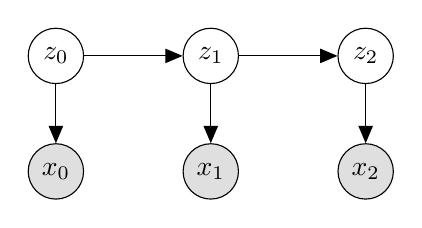
\begin{tikzpicture}[]
\node[latent] (z0) {$z_0$} ;
\node[latent] (z1) [right=1.25cm of z0] {$z_1$} ;
\node[latent] (z2) [right=1.25cm of z1] {$z_2$} ;

\node[obs]    (x0) [below = 0.75cm of z0] {$x_0$};
\node[obs]    (x1) [below = 0.75cm of z1] {$x_1$};
\node[obs]    (x2) [below = 0.75cm of z2] {$x_2$};

\edge {z0} {x0};
\edge {z1} {x1};
\edge {z2} {x2};
\edge {z0} {z1};
\edge {z1} {z2};
\end{tikzpicture}
\end{center}

%\begin{equation*}
%p(\bx,\bz) = \prod_{t=1}^T 
    %\underbrace{p(z_t \mid z_{t-1})}_{\textrm{transition}}
    %\underbrace{p(x_t\mid z_t)}_{\textrm{emission}}
%\end{equation*}
\vspace{1em}
We wish to optimize
\begin{equation*}
p(x) = \sum_z p(x,z),
\end{equation*}
computed via the forward algorithm
\end{frame}

\begin{frame}
\frametitle{3 Techniques for Training Large HMMs}
\begin{itemize}
\item Block-sparse emission constraints
\vspace{1em}
    \begin{itemize}
    \item[] \FancyUpArrow~Speed
    \end{itemize}
\vspace{1em}
\item Compact neural parameterization
\vspace{1em}
    \begin{itemize}
    \item[] \FancyUpArrow~Generalization
    \end{itemize}
\vspace{1em}
\item State dropout
\vspace{1em}
    \begin{itemize}
    \item[] \FancyUpArrow~Speed \quad \FancyUpArrow~Generalization
    \end{itemize}
\end{itemize}
\end{frame}

\begin{frame}
\frametitle{Technique 1: Block-Sparse Emission Constraints}
\begin{itemize}
\item Reduce cost of marginalization by enforcing structure
\vspace{0.5em}
\item Partition words and states jointly
\vspace{0.5em}
\item Words can only be emit by states in same group
\end{itemize}
\begin{center}
\begin{tikzpicture}[every node/.style={anchor=base,minimum size=8mm}]
    \matrix  (graph) [matrix of nodes, row sep=0.5em,column sep=-0.3em,
    minimum width=2em, minimum height=2em, font=\small,ampersand replacement=\&,
    nodes in empty cells
    ] {
        \&$\mcX_1$ \&
        \&
        \textcolor{green!10}{a}\&
        $\mcX_2$ \&
        \textcolor{green!10}{a}\&
        \&
        $\cdots$ \&
        \&
        $\mcX_M$ \\
        \textcolor{blue!80}{$p(x\mid z)$} \& \& \& \&\& \&\&\&\&\\
        \&$\mcZ_1$ \&
        \&
        $\mcZ_2$ \&
        \&
        $\cdots$ \&
        \&
        $\mcZ_M$ \&\&\\
    };
    
    \begin{scope}[on background layer]
      \draw[blue!30, line width=0.5mm] (graph-1-2) -- (graph-3-2);
      \draw[blue!30,line width=0.5mm] (graph-1-5) -- (graph-3-4);
      \draw[blue!30,line width=0.5mm] (graph-1-10) -- (graph-3-8);

      %\draw[draw=red!30, line width=0.2mm] ($(graph-1-1) + (0.1, 0)$) -- ($(graph-3-3) + (0.1, 0)$);
      %\draw[draw=red!30, line width=0.2mm] ($(graph-1-2) + (0.1, 0)$) -- ($(graph-3-3) + (0.1, 0)$);
      %\draw[draw=red!30, line width=0.1mm] ($(graph-1-3) + (0.1, 0)$) -- ($(graph-3-3) + (0.1, 0)$);
      %\draw[draw=red!30, line width=0.9mm] ($(graph-1-4) + (0.1, 0)$) -- ($(graph-3-3) + (0.1, 0)$);
      %\draw[draw=red!30, line width=0.1mm] ($(graph-1-5) + (0.1, 0)$) -- ($(graph-3-3) + (0.1, 0)$);
      %\draw[draw=red!30, line width=0.4mm] ($(graph-1-6) + (0.1, 0)$) -- ($(graph-3-3) + (0.1, 0)$);
      %\draw[draw=red!30, line width=0.1mm] ($(graph-1-7) + (0.1, 0)$) -- ($(graph-3-3) + (0.1, 0)$);

      \draw[rounded corners,fill=red!10] ($ (graph-3-2.north west) +(-0.1,0.1)$) rectangle  node[yshift=-0.8cm]{\textcolor{red}{}} ($(graph-3-8.south east) +(0.1,-0.1)$ ) ;
      \draw[rounded corners,fill=red!10] ($ (graph-1-2.north west) +(-0.1,0.1)$) rectangle  node[yshift=0.8cm]{\textcolor{red}{}} ($(graph-1-10.south east) +(0.1,-0.1)$ ) ;

      \draw[rounded corners,fill=green!10] (graph-1-2.north west) rectangle  node[ yshift =0.7cm] {} (graph-1-2.south east);
      \draw[rounded corners,fill=green!10] (graph-1-4.north west) rectangle  node[ yshift =0.7cm] {} (graph-1-6.south east);
      \draw[rounded corners,fill=green!10] (graph-1-10.north west) rectangle  node[ yshift =0.7cm] {} (graph-1-10.south east);

      \draw[rounded corners, fill=blue!10] (graph-3-2.north west) rectangle  node[yshift=-0.9cm]{}  ($(graph-3-2.south east)$);
      \draw[rounded corners, fill=blue!10] (graph-3-4.north west) rectangle  node[yshift=-0.9cm]{}  ($(graph-3-4.south east)$);
      \draw[rounded corners,fill=blue!10] (graph-3-8.north west) rectangle  node[ yshift =0.7cm] {} (graph-3-8.south east);
      %\path[] (graph-3-3.north west) rectangle  node[yshift=-0.9cm]{\textbf{$y_3$}} (graph-3-3.south east);
    \end{scope}
  \end{tikzpicture}
\end{center}

\end{frame}

\begin{frame}
\frametitle{Block-Sparse Emissions: Effect on Inference}

Given each word $x_t$, only the states in the correct group can occur
\vspace{1em} 

\begin{figure}
\captionsetup[subfigure]{justification=centering}
\begin{center}
\begin{subfigure}[t]{0.45\textwidth}
\centering
\resizebox{0.75\width}{0.75\height}{
\normalsize%
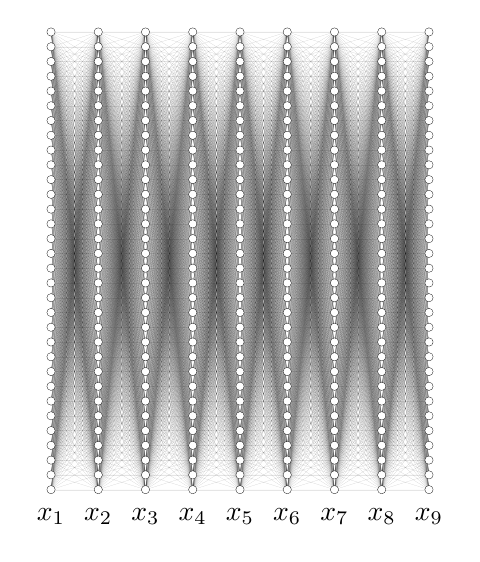
\begin{tikzpicture}%
\path[draw,line width=0.1pt,opacity=0.1,fill=black] (0.6,0.0) -- (1.2,0.0);%
\path[draw,line width=0.1pt,opacity=0.1,fill=black] (0.6,0.0) -- (1.2,0.1875);%
\path[draw,line width=0.1pt,opacity=0.1,fill=black] (0.6,0.0) -- (1.2,0.375);%
\path[draw,line width=0.1pt,opacity=0.1,fill=black] (0.6,0.0) -- (1.2,0.5625);%
\path[draw,line width=0.1pt,opacity=0.1,fill=black] (0.6,0.0) -- (1.2,0.75);%
\path[draw,line width=0.1pt,opacity=0.1,fill=black] (0.6,0.0) -- (1.2,0.9375);%
\path[draw,line width=0.1pt,opacity=0.1,fill=black] (0.6,0.0) -- (1.2,1.125);%
\path[draw,line width=0.1pt,opacity=0.1,fill=black] (0.6,0.0) -- (1.2,1.3125);%
\path[draw,line width=0.1pt,opacity=0.1,fill=black] (0.6,0.0) -- (1.2,1.5);%
\path[draw,line width=0.1pt,opacity=0.1,fill=black] (0.6,0.0) -- (1.2,1.6875);%
\path[draw,line width=0.1pt,opacity=0.1,fill=black] (0.6,0.0) -- (1.2,1.875);%
\path[draw,line width=0.1pt,opacity=0.1,fill=black] (0.6,0.0) -- (1.2,2.0625);%
\path[draw,line width=0.1pt,opacity=0.1,fill=black] (0.6,0.0) -- (1.2,2.25);%
\path[draw,line width=0.1pt,opacity=0.1,fill=black] (0.6,0.0) -- (1.2,2.4375);%
\path[draw,line width=0.1pt,opacity=0.1,fill=black] (0.6,0.0) -- (1.2,2.625);%
\path[draw,line width=0.1pt,opacity=0.1,fill=black] (0.6,0.0) -- (1.2,2.8125);%
\path[draw,line width=0.1pt,opacity=0.1,fill=black] (0.6,0.0) -- (1.2,3.0);%
\path[draw,line width=0.1pt,opacity=0.1,fill=black] (0.6,0.0) -- (1.2,3.1875);%
\path[draw,line width=0.1pt,opacity=0.1,fill=black] (0.6,0.0) -- (1.2,3.375);%
\path[draw,line width=0.1pt,opacity=0.1,fill=black] (0.6,0.0) -- (1.2,3.5625);%
\path[draw,line width=0.1pt,opacity=0.1,fill=black] (0.6,0.0) -- (1.2,3.75);%
\path[draw,line width=0.1pt,opacity=0.1,fill=black] (0.6,0.0) -- (1.2,3.9375);%
\path[draw,line width=0.1pt,opacity=0.1,fill=black] (0.6,0.0) -- (1.2,4.125);%
\path[draw,line width=0.1pt,opacity=0.1,fill=black] (0.6,0.0) -- (1.2,4.3125);%
\path[draw,line width=0.1pt,opacity=0.1,fill=black] (0.6,0.0) -- (1.2,4.5);%
\path[draw,line width=0.1pt,opacity=0.1,fill=black] (0.6,0.0) -- (1.2,4.6875);%
\path[draw,line width=0.1pt,opacity=0.1,fill=black] (0.6,0.0) -- (1.2,4.875);%
\path[draw,line width=0.1pt,opacity=0.1,fill=black] (0.6,0.0) -- (1.2,5.0625);%
\path[draw,line width=0.1pt,opacity=0.1,fill=black] (0.6,0.0) -- (1.2,5.25);%
\path[draw,line width=0.1pt,opacity=0.1,fill=black] (0.6,0.0) -- (1.2,5.4375);%
\path[draw,line width=0.1pt,opacity=0.1,fill=black] (0.6,0.0) -- (1.2,5.625);%
\path[draw,line width=0.1pt,opacity=0.1,fill=black] (0.6,0.0) -- (1.2,5.8125);%
\path[draw,line width=0.1pt,opacity=0.1,fill=black] (0.6,0.1875) -- (1.2,0.0);%
\path[draw,line width=0.1pt,opacity=0.1,fill=black] (0.6,0.1875) -- (1.2,0.1875);%
\path[draw,line width=0.1pt,opacity=0.1,fill=black] (0.6,0.1875) -- (1.2,0.375);%
\path[draw,line width=0.1pt,opacity=0.1,fill=black] (0.6,0.1875) -- (1.2,0.5625);%
\path[draw,line width=0.1pt,opacity=0.1,fill=black] (0.6,0.1875) -- (1.2,0.75);%
\path[draw,line width=0.1pt,opacity=0.1,fill=black] (0.6,0.1875) -- (1.2,0.9375);%
\path[draw,line width=0.1pt,opacity=0.1,fill=black] (0.6,0.1875) -- (1.2,1.125);%
\path[draw,line width=0.1pt,opacity=0.1,fill=black] (0.6,0.1875) -- (1.2,1.3125);%
\path[draw,line width=0.1pt,opacity=0.1,fill=black] (0.6,0.1875) -- (1.2,1.5);%
\path[draw,line width=0.1pt,opacity=0.1,fill=black] (0.6,0.1875) -- (1.2,1.6875);%
\path[draw,line width=0.1pt,opacity=0.1,fill=black] (0.6,0.1875) -- (1.2,1.875);%
\path[draw,line width=0.1pt,opacity=0.1,fill=black] (0.6,0.1875) -- (1.2,2.0625);%
\path[draw,line width=0.1pt,opacity=0.1,fill=black] (0.6,0.1875) -- (1.2,2.25);%
\path[draw,line width=0.1pt,opacity=0.1,fill=black] (0.6,0.1875) -- (1.2,2.4375);%
\path[draw,line width=0.1pt,opacity=0.1,fill=black] (0.6,0.1875) -- (1.2,2.625);%
\path[draw,line width=0.1pt,opacity=0.1,fill=black] (0.6,0.1875) -- (1.2,2.8125);%
\path[draw,line width=0.1pt,opacity=0.1,fill=black] (0.6,0.1875) -- (1.2,3.0);%
\path[draw,line width=0.1pt,opacity=0.1,fill=black] (0.6,0.1875) -- (1.2,3.1875);%
\path[draw,line width=0.1pt,opacity=0.1,fill=black] (0.6,0.1875) -- (1.2,3.375);%
\path[draw,line width=0.1pt,opacity=0.1,fill=black] (0.6,0.1875) -- (1.2,3.5625);%
\path[draw,line width=0.1pt,opacity=0.1,fill=black] (0.6,0.1875) -- (1.2,3.75);%
\path[draw,line width=0.1pt,opacity=0.1,fill=black] (0.6,0.1875) -- (1.2,3.9375);%
\path[draw,line width=0.1pt,opacity=0.1,fill=black] (0.6,0.1875) -- (1.2,4.125);%
\path[draw,line width=0.1pt,opacity=0.1,fill=black] (0.6,0.1875) -- (1.2,4.3125);%
\path[draw,line width=0.1pt,opacity=0.1,fill=black] (0.6,0.1875) -- (1.2,4.5);%
\path[draw,line width=0.1pt,opacity=0.1,fill=black] (0.6,0.1875) -- (1.2,4.6875);%
\path[draw,line width=0.1pt,opacity=0.1,fill=black] (0.6,0.1875) -- (1.2,4.875);%
\path[draw,line width=0.1pt,opacity=0.1,fill=black] (0.6,0.1875) -- (1.2,5.0625);%
\path[draw,line width=0.1pt,opacity=0.1,fill=black] (0.6,0.1875) -- (1.2,5.25);%
\path[draw,line width=0.1pt,opacity=0.1,fill=black] (0.6,0.1875) -- (1.2,5.4375);%
\path[draw,line width=0.1pt,opacity=0.1,fill=black] (0.6,0.1875) -- (1.2,5.625);%
\path[draw,line width=0.1pt,opacity=0.1,fill=black] (0.6,0.1875) -- (1.2,5.8125);%
\path[draw,line width=0.1pt,opacity=0.1,fill=black] (0.6,0.375) -- (1.2,0.0);%
\path[draw,line width=0.1pt,opacity=0.1,fill=black] (0.6,0.375) -- (1.2,0.1875);%
\path[draw,line width=0.1pt,opacity=0.1,fill=black] (0.6,0.375) -- (1.2,0.375);%
\path[draw,line width=0.1pt,opacity=0.1,fill=black] (0.6,0.375) -- (1.2,0.5625);%
\path[draw,line width=0.1pt,opacity=0.1,fill=black] (0.6,0.375) -- (1.2,0.75);%
\path[draw,line width=0.1pt,opacity=0.1,fill=black] (0.6,0.375) -- (1.2,0.9375);%
\path[draw,line width=0.1pt,opacity=0.1,fill=black] (0.6,0.375) -- (1.2,1.125);%
\path[draw,line width=0.1pt,opacity=0.1,fill=black] (0.6,0.375) -- (1.2,1.3125);%
\path[draw,line width=0.1pt,opacity=0.1,fill=black] (0.6,0.375) -- (1.2,1.5);%
\path[draw,line width=0.1pt,opacity=0.1,fill=black] (0.6,0.375) -- (1.2,1.6875);%
\path[draw,line width=0.1pt,opacity=0.1,fill=black] (0.6,0.375) -- (1.2,1.875);%
\path[draw,line width=0.1pt,opacity=0.1,fill=black] (0.6,0.375) -- (1.2,2.0625);%
\path[draw,line width=0.1pt,opacity=0.1,fill=black] (0.6,0.375) -- (1.2,2.25);%
\path[draw,line width=0.1pt,opacity=0.1,fill=black] (0.6,0.375) -- (1.2,2.4375);%
\path[draw,line width=0.1pt,opacity=0.1,fill=black] (0.6,0.375) -- (1.2,2.625);%
\path[draw,line width=0.1pt,opacity=0.1,fill=black] (0.6,0.375) -- (1.2,2.8125);%
\path[draw,line width=0.1pt,opacity=0.1,fill=black] (0.6,0.375) -- (1.2,3.0);%
\path[draw,line width=0.1pt,opacity=0.1,fill=black] (0.6,0.375) -- (1.2,3.1875);%
\path[draw,line width=0.1pt,opacity=0.1,fill=black] (0.6,0.375) -- (1.2,3.375);%
\path[draw,line width=0.1pt,opacity=0.1,fill=black] (0.6,0.375) -- (1.2,3.5625);%
\path[draw,line width=0.1pt,opacity=0.1,fill=black] (0.6,0.375) -- (1.2,3.75);%
\path[draw,line width=0.1pt,opacity=0.1,fill=black] (0.6,0.375) -- (1.2,3.9375);%
\path[draw,line width=0.1pt,opacity=0.1,fill=black] (0.6,0.375) -- (1.2,4.125);%
\path[draw,line width=0.1pt,opacity=0.1,fill=black] (0.6,0.375) -- (1.2,4.3125);%
\path[draw,line width=0.1pt,opacity=0.1,fill=black] (0.6,0.375) -- (1.2,4.5);%
\path[draw,line width=0.1pt,opacity=0.1,fill=black] (0.6,0.375) -- (1.2,4.6875);%
\path[draw,line width=0.1pt,opacity=0.1,fill=black] (0.6,0.375) -- (1.2,4.875);%
\path[draw,line width=0.1pt,opacity=0.1,fill=black] (0.6,0.375) -- (1.2,5.0625);%
\path[draw,line width=0.1pt,opacity=0.1,fill=black] (0.6,0.375) -- (1.2,5.25);%
\path[draw,line width=0.1pt,opacity=0.1,fill=black] (0.6,0.375) -- (1.2,5.4375);%
\path[draw,line width=0.1pt,opacity=0.1,fill=black] (0.6,0.375) -- (1.2,5.625);%
\path[draw,line width=0.1pt,opacity=0.1,fill=black] (0.6,0.375) -- (1.2,5.8125);%
\path[draw,line width=0.1pt,opacity=0.1,fill=black] (0.6,0.5625) -- (1.2,0.0);%
\path[draw,line width=0.1pt,opacity=0.1,fill=black] (0.6,0.5625) -- (1.2,0.1875);%
\path[draw,line width=0.1pt,opacity=0.1,fill=black] (0.6,0.5625) -- (1.2,0.375);%
\path[draw,line width=0.1pt,opacity=0.1,fill=black] (0.6,0.5625) -- (1.2,0.5625);%
\path[draw,line width=0.1pt,opacity=0.1,fill=black] (0.6,0.5625) -- (1.2,0.75);%
\path[draw,line width=0.1pt,opacity=0.1,fill=black] (0.6,0.5625) -- (1.2,0.9375);%
\path[draw,line width=0.1pt,opacity=0.1,fill=black] (0.6,0.5625) -- (1.2,1.125);%
\path[draw,line width=0.1pt,opacity=0.1,fill=black] (0.6,0.5625) -- (1.2,1.3125);%
\path[draw,line width=0.1pt,opacity=0.1,fill=black] (0.6,0.5625) -- (1.2,1.5);%
\path[draw,line width=0.1pt,opacity=0.1,fill=black] (0.6,0.5625) -- (1.2,1.6875);%
\path[draw,line width=0.1pt,opacity=0.1,fill=black] (0.6,0.5625) -- (1.2,1.875);%
\path[draw,line width=0.1pt,opacity=0.1,fill=black] (0.6,0.5625) -- (1.2,2.0625);%
\path[draw,line width=0.1pt,opacity=0.1,fill=black] (0.6,0.5625) -- (1.2,2.25);%
\path[draw,line width=0.1pt,opacity=0.1,fill=black] (0.6,0.5625) -- (1.2,2.4375);%
\path[draw,line width=0.1pt,opacity=0.1,fill=black] (0.6,0.5625) -- (1.2,2.625);%
\path[draw,line width=0.1pt,opacity=0.1,fill=black] (0.6,0.5625) -- (1.2,2.8125);%
\path[draw,line width=0.1pt,opacity=0.1,fill=black] (0.6,0.5625) -- (1.2,3.0);%
\path[draw,line width=0.1pt,opacity=0.1,fill=black] (0.6,0.5625) -- (1.2,3.1875);%
\path[draw,line width=0.1pt,opacity=0.1,fill=black] (0.6,0.5625) -- (1.2,3.375);%
\path[draw,line width=0.1pt,opacity=0.1,fill=black] (0.6,0.5625) -- (1.2,3.5625);%
\path[draw,line width=0.1pt,opacity=0.1,fill=black] (0.6,0.5625) -- (1.2,3.75);%
\path[draw,line width=0.1pt,opacity=0.1,fill=black] (0.6,0.5625) -- (1.2,3.9375);%
\path[draw,line width=0.1pt,opacity=0.1,fill=black] (0.6,0.5625) -- (1.2,4.125);%
\path[draw,line width=0.1pt,opacity=0.1,fill=black] (0.6,0.5625) -- (1.2,4.3125);%
\path[draw,line width=0.1pt,opacity=0.1,fill=black] (0.6,0.5625) -- (1.2,4.5);%
\path[draw,line width=0.1pt,opacity=0.1,fill=black] (0.6,0.5625) -- (1.2,4.6875);%
\path[draw,line width=0.1pt,opacity=0.1,fill=black] (0.6,0.5625) -- (1.2,4.875);%
\path[draw,line width=0.1pt,opacity=0.1,fill=black] (0.6,0.5625) -- (1.2,5.0625);%
\path[draw,line width=0.1pt,opacity=0.1,fill=black] (0.6,0.5625) -- (1.2,5.25);%
\path[draw,line width=0.1pt,opacity=0.1,fill=black] (0.6,0.5625) -- (1.2,5.4375);%
\path[draw,line width=0.1pt,opacity=0.1,fill=black] (0.6,0.5625) -- (1.2,5.625);%
\path[draw,line width=0.1pt,opacity=0.1,fill=black] (0.6,0.5625) -- (1.2,5.8125);%
\path[draw,line width=0.1pt,opacity=0.1,fill=black] (0.6,0.75) -- (1.2,0.0);%
\path[draw,line width=0.1pt,opacity=0.1,fill=black] (0.6,0.75) -- (1.2,0.1875);%
\path[draw,line width=0.1pt,opacity=0.1,fill=black] (0.6,0.75) -- (1.2,0.375);%
\path[draw,line width=0.1pt,opacity=0.1,fill=black] (0.6,0.75) -- (1.2,0.5625);%
\path[draw,line width=0.1pt,opacity=0.1,fill=black] (0.6,0.75) -- (1.2,0.75);%
\path[draw,line width=0.1pt,opacity=0.1,fill=black] (0.6,0.75) -- (1.2,0.9375);%
\path[draw,line width=0.1pt,opacity=0.1,fill=black] (0.6,0.75) -- (1.2,1.125);%
\path[draw,line width=0.1pt,opacity=0.1,fill=black] (0.6,0.75) -- (1.2,1.3125);%
\path[draw,line width=0.1pt,opacity=0.1,fill=black] (0.6,0.75) -- (1.2,1.5);%
\path[draw,line width=0.1pt,opacity=0.1,fill=black] (0.6,0.75) -- (1.2,1.6875);%
\path[draw,line width=0.1pt,opacity=0.1,fill=black] (0.6,0.75) -- (1.2,1.875);%
\path[draw,line width=0.1pt,opacity=0.1,fill=black] (0.6,0.75) -- (1.2,2.0625);%
\path[draw,line width=0.1pt,opacity=0.1,fill=black] (0.6,0.75) -- (1.2,2.25);%
\path[draw,line width=0.1pt,opacity=0.1,fill=black] (0.6,0.75) -- (1.2,2.4375);%
\path[draw,line width=0.1pt,opacity=0.1,fill=black] (0.6,0.75) -- (1.2,2.625);%
\path[draw,line width=0.1pt,opacity=0.1,fill=black] (0.6,0.75) -- (1.2,2.8125);%
\path[draw,line width=0.1pt,opacity=0.1,fill=black] (0.6,0.75) -- (1.2,3.0);%
\path[draw,line width=0.1pt,opacity=0.1,fill=black] (0.6,0.75) -- (1.2,3.1875);%
\path[draw,line width=0.1pt,opacity=0.1,fill=black] (0.6,0.75) -- (1.2,3.375);%
\path[draw,line width=0.1pt,opacity=0.1,fill=black] (0.6,0.75) -- (1.2,3.5625);%
\path[draw,line width=0.1pt,opacity=0.1,fill=black] (0.6,0.75) -- (1.2,3.75);%
\path[draw,line width=0.1pt,opacity=0.1,fill=black] (0.6,0.75) -- (1.2,3.9375);%
\path[draw,line width=0.1pt,opacity=0.1,fill=black] (0.6,0.75) -- (1.2,4.125);%
\path[draw,line width=0.1pt,opacity=0.1,fill=black] (0.6,0.75) -- (1.2,4.3125);%
\path[draw,line width=0.1pt,opacity=0.1,fill=black] (0.6,0.75) -- (1.2,4.5);%
\path[draw,line width=0.1pt,opacity=0.1,fill=black] (0.6,0.75) -- (1.2,4.6875);%
\path[draw,line width=0.1pt,opacity=0.1,fill=black] (0.6,0.75) -- (1.2,4.875);%
\path[draw,line width=0.1pt,opacity=0.1,fill=black] (0.6,0.75) -- (1.2,5.0625);%
\path[draw,line width=0.1pt,opacity=0.1,fill=black] (0.6,0.75) -- (1.2,5.25);%
\path[draw,line width=0.1pt,opacity=0.1,fill=black] (0.6,0.75) -- (1.2,5.4375);%
\path[draw,line width=0.1pt,opacity=0.1,fill=black] (0.6,0.75) -- (1.2,5.625);%
\path[draw,line width=0.1pt,opacity=0.1,fill=black] (0.6,0.75) -- (1.2,5.8125);%
\path[draw,line width=0.1pt,opacity=0.1,fill=black] (0.6,0.9375) -- (1.2,0.0);%
\path[draw,line width=0.1pt,opacity=0.1,fill=black] (0.6,0.9375) -- (1.2,0.1875);%
\path[draw,line width=0.1pt,opacity=0.1,fill=black] (0.6,0.9375) -- (1.2,0.375);%
\path[draw,line width=0.1pt,opacity=0.1,fill=black] (0.6,0.9375) -- (1.2,0.5625);%
\path[draw,line width=0.1pt,opacity=0.1,fill=black] (0.6,0.9375) -- (1.2,0.75);%
\path[draw,line width=0.1pt,opacity=0.1,fill=black] (0.6,0.9375) -- (1.2,0.9375);%
\path[draw,line width=0.1pt,opacity=0.1,fill=black] (0.6,0.9375) -- (1.2,1.125);%
\path[draw,line width=0.1pt,opacity=0.1,fill=black] (0.6,0.9375) -- (1.2,1.3125);%
\path[draw,line width=0.1pt,opacity=0.1,fill=black] (0.6,0.9375) -- (1.2,1.5);%
\path[draw,line width=0.1pt,opacity=0.1,fill=black] (0.6,0.9375) -- (1.2,1.6875);%
\path[draw,line width=0.1pt,opacity=0.1,fill=black] (0.6,0.9375) -- (1.2,1.875);%
\path[draw,line width=0.1pt,opacity=0.1,fill=black] (0.6,0.9375) -- (1.2,2.0625);%
\path[draw,line width=0.1pt,opacity=0.1,fill=black] (0.6,0.9375) -- (1.2,2.25);%
\path[draw,line width=0.1pt,opacity=0.1,fill=black] (0.6,0.9375) -- (1.2,2.4375);%
\path[draw,line width=0.1pt,opacity=0.1,fill=black] (0.6,0.9375) -- (1.2,2.625);%
\path[draw,line width=0.1pt,opacity=0.1,fill=black] (0.6,0.9375) -- (1.2,2.8125);%
\path[draw,line width=0.1pt,opacity=0.1,fill=black] (0.6,0.9375) -- (1.2,3.0);%
\path[draw,line width=0.1pt,opacity=0.1,fill=black] (0.6,0.9375) -- (1.2,3.1875);%
\path[draw,line width=0.1pt,opacity=0.1,fill=black] (0.6,0.9375) -- (1.2,3.375);%
\path[draw,line width=0.1pt,opacity=0.1,fill=black] (0.6,0.9375) -- (1.2,3.5625);%
\path[draw,line width=0.1pt,opacity=0.1,fill=black] (0.6,0.9375) -- (1.2,3.75);%
\path[draw,line width=0.1pt,opacity=0.1,fill=black] (0.6,0.9375) -- (1.2,3.9375);%
\path[draw,line width=0.1pt,opacity=0.1,fill=black] (0.6,0.9375) -- (1.2,4.125);%
\path[draw,line width=0.1pt,opacity=0.1,fill=black] (0.6,0.9375) -- (1.2,4.3125);%
\path[draw,line width=0.1pt,opacity=0.1,fill=black] (0.6,0.9375) -- (1.2,4.5);%
\path[draw,line width=0.1pt,opacity=0.1,fill=black] (0.6,0.9375) -- (1.2,4.6875);%
\path[draw,line width=0.1pt,opacity=0.1,fill=black] (0.6,0.9375) -- (1.2,4.875);%
\path[draw,line width=0.1pt,opacity=0.1,fill=black] (0.6,0.9375) -- (1.2,5.0625);%
\path[draw,line width=0.1pt,opacity=0.1,fill=black] (0.6,0.9375) -- (1.2,5.25);%
\path[draw,line width=0.1pt,opacity=0.1,fill=black] (0.6,0.9375) -- (1.2,5.4375);%
\path[draw,line width=0.1pt,opacity=0.1,fill=black] (0.6,0.9375) -- (1.2,5.625);%
\path[draw,line width=0.1pt,opacity=0.1,fill=black] (0.6,0.9375) -- (1.2,5.8125);%
\path[draw,line width=0.1pt,opacity=0.1,fill=black] (0.6,1.125) -- (1.2,0.0);%
\path[draw,line width=0.1pt,opacity=0.1,fill=black] (0.6,1.125) -- (1.2,0.1875);%
\path[draw,line width=0.1pt,opacity=0.1,fill=black] (0.6,1.125) -- (1.2,0.375);%
\path[draw,line width=0.1pt,opacity=0.1,fill=black] (0.6,1.125) -- (1.2,0.5625);%
\path[draw,line width=0.1pt,opacity=0.1,fill=black] (0.6,1.125) -- (1.2,0.75);%
\path[draw,line width=0.1pt,opacity=0.1,fill=black] (0.6,1.125) -- (1.2,0.9375);%
\path[draw,line width=0.1pt,opacity=0.1,fill=black] (0.6,1.125) -- (1.2,1.125);%
\path[draw,line width=0.1pt,opacity=0.1,fill=black] (0.6,1.125) -- (1.2,1.3125);%
\path[draw,line width=0.1pt,opacity=0.1,fill=black] (0.6,1.125) -- (1.2,1.5);%
\path[draw,line width=0.1pt,opacity=0.1,fill=black] (0.6,1.125) -- (1.2,1.6875);%
\path[draw,line width=0.1pt,opacity=0.1,fill=black] (0.6,1.125) -- (1.2,1.875);%
\path[draw,line width=0.1pt,opacity=0.1,fill=black] (0.6,1.125) -- (1.2,2.0625);%
\path[draw,line width=0.1pt,opacity=0.1,fill=black] (0.6,1.125) -- (1.2,2.25);%
\path[draw,line width=0.1pt,opacity=0.1,fill=black] (0.6,1.125) -- (1.2,2.4375);%
\path[draw,line width=0.1pt,opacity=0.1,fill=black] (0.6,1.125) -- (1.2,2.625);%
\path[draw,line width=0.1pt,opacity=0.1,fill=black] (0.6,1.125) -- (1.2,2.8125);%
\path[draw,line width=0.1pt,opacity=0.1,fill=black] (0.6,1.125) -- (1.2,3.0);%
\path[draw,line width=0.1pt,opacity=0.1,fill=black] (0.6,1.125) -- (1.2,3.1875);%
\path[draw,line width=0.1pt,opacity=0.1,fill=black] (0.6,1.125) -- (1.2,3.375);%
\path[draw,line width=0.1pt,opacity=0.1,fill=black] (0.6,1.125) -- (1.2,3.5625);%
\path[draw,line width=0.1pt,opacity=0.1,fill=black] (0.6,1.125) -- (1.2,3.75);%
\path[draw,line width=0.1pt,opacity=0.1,fill=black] (0.6,1.125) -- (1.2,3.9375);%
\path[draw,line width=0.1pt,opacity=0.1,fill=black] (0.6,1.125) -- (1.2,4.125);%
\path[draw,line width=0.1pt,opacity=0.1,fill=black] (0.6,1.125) -- (1.2,4.3125);%
\path[draw,line width=0.1pt,opacity=0.1,fill=black] (0.6,1.125) -- (1.2,4.5);%
\path[draw,line width=0.1pt,opacity=0.1,fill=black] (0.6,1.125) -- (1.2,4.6875);%
\path[draw,line width=0.1pt,opacity=0.1,fill=black] (0.6,1.125) -- (1.2,4.875);%
\path[draw,line width=0.1pt,opacity=0.1,fill=black] (0.6,1.125) -- (1.2,5.0625);%
\path[draw,line width=0.1pt,opacity=0.1,fill=black] (0.6,1.125) -- (1.2,5.25);%
\path[draw,line width=0.1pt,opacity=0.1,fill=black] (0.6,1.125) -- (1.2,5.4375);%
\path[draw,line width=0.1pt,opacity=0.1,fill=black] (0.6,1.125) -- (1.2,5.625);%
\path[draw,line width=0.1pt,opacity=0.1,fill=black] (0.6,1.125) -- (1.2,5.8125);%
\path[draw,line width=0.1pt,opacity=0.1,fill=black] (0.6,1.3125) -- (1.2,0.0);%
\path[draw,line width=0.1pt,opacity=0.1,fill=black] (0.6,1.3125) -- (1.2,0.1875);%
\path[draw,line width=0.1pt,opacity=0.1,fill=black] (0.6,1.3125) -- (1.2,0.375);%
\path[draw,line width=0.1pt,opacity=0.1,fill=black] (0.6,1.3125) -- (1.2,0.5625);%
\path[draw,line width=0.1pt,opacity=0.1,fill=black] (0.6,1.3125) -- (1.2,0.75);%
\path[draw,line width=0.1pt,opacity=0.1,fill=black] (0.6,1.3125) -- (1.2,0.9375);%
\path[draw,line width=0.1pt,opacity=0.1,fill=black] (0.6,1.3125) -- (1.2,1.125);%
\path[draw,line width=0.1pt,opacity=0.1,fill=black] (0.6,1.3125) -- (1.2,1.3125);%
\path[draw,line width=0.1pt,opacity=0.1,fill=black] (0.6,1.3125) -- (1.2,1.5);%
\path[draw,line width=0.1pt,opacity=0.1,fill=black] (0.6,1.3125) -- (1.2,1.6875);%
\path[draw,line width=0.1pt,opacity=0.1,fill=black] (0.6,1.3125) -- (1.2,1.875);%
\path[draw,line width=0.1pt,opacity=0.1,fill=black] (0.6,1.3125) -- (1.2,2.0625);%
\path[draw,line width=0.1pt,opacity=0.1,fill=black] (0.6,1.3125) -- (1.2,2.25);%
\path[draw,line width=0.1pt,opacity=0.1,fill=black] (0.6,1.3125) -- (1.2,2.4375);%
\path[draw,line width=0.1pt,opacity=0.1,fill=black] (0.6,1.3125) -- (1.2,2.625);%
\path[draw,line width=0.1pt,opacity=0.1,fill=black] (0.6,1.3125) -- (1.2,2.8125);%
\path[draw,line width=0.1pt,opacity=0.1,fill=black] (0.6,1.3125) -- (1.2,3.0);%
\path[draw,line width=0.1pt,opacity=0.1,fill=black] (0.6,1.3125) -- (1.2,3.1875);%
\path[draw,line width=0.1pt,opacity=0.1,fill=black] (0.6,1.3125) -- (1.2,3.375);%
\path[draw,line width=0.1pt,opacity=0.1,fill=black] (0.6,1.3125) -- (1.2,3.5625);%
\path[draw,line width=0.1pt,opacity=0.1,fill=black] (0.6,1.3125) -- (1.2,3.75);%
\path[draw,line width=0.1pt,opacity=0.1,fill=black] (0.6,1.3125) -- (1.2,3.9375);%
\path[draw,line width=0.1pt,opacity=0.1,fill=black] (0.6,1.3125) -- (1.2,4.125);%
\path[draw,line width=0.1pt,opacity=0.1,fill=black] (0.6,1.3125) -- (1.2,4.3125);%
\path[draw,line width=0.1pt,opacity=0.1,fill=black] (0.6,1.3125) -- (1.2,4.5);%
\path[draw,line width=0.1pt,opacity=0.1,fill=black] (0.6,1.3125) -- (1.2,4.6875);%
\path[draw,line width=0.1pt,opacity=0.1,fill=black] (0.6,1.3125) -- (1.2,4.875);%
\path[draw,line width=0.1pt,opacity=0.1,fill=black] (0.6,1.3125) -- (1.2,5.0625);%
\path[draw,line width=0.1pt,opacity=0.1,fill=black] (0.6,1.3125) -- (1.2,5.25);%
\path[draw,line width=0.1pt,opacity=0.1,fill=black] (0.6,1.3125) -- (1.2,5.4375);%
\path[draw,line width=0.1pt,opacity=0.1,fill=black] (0.6,1.3125) -- (1.2,5.625);%
\path[draw,line width=0.1pt,opacity=0.1,fill=black] (0.6,1.3125) -- (1.2,5.8125);%
\path[draw,line width=0.1pt,opacity=0.1,fill=black] (0.6,1.5) -- (1.2,0.0);%
\path[draw,line width=0.1pt,opacity=0.1,fill=black] (0.6,1.5) -- (1.2,0.1875);%
\path[draw,line width=0.1pt,opacity=0.1,fill=black] (0.6,1.5) -- (1.2,0.375);%
\path[draw,line width=0.1pt,opacity=0.1,fill=black] (0.6,1.5) -- (1.2,0.5625);%
\path[draw,line width=0.1pt,opacity=0.1,fill=black] (0.6,1.5) -- (1.2,0.75);%
\path[draw,line width=0.1pt,opacity=0.1,fill=black] (0.6,1.5) -- (1.2,0.9375);%
\path[draw,line width=0.1pt,opacity=0.1,fill=black] (0.6,1.5) -- (1.2,1.125);%
\path[draw,line width=0.1pt,opacity=0.1,fill=black] (0.6,1.5) -- (1.2,1.3125);%
\path[draw,line width=0.1pt,opacity=0.1,fill=black] (0.6,1.5) -- (1.2,1.5);%
\path[draw,line width=0.1pt,opacity=0.1,fill=black] (0.6,1.5) -- (1.2,1.6875);%
\path[draw,line width=0.1pt,opacity=0.1,fill=black] (0.6,1.5) -- (1.2,1.875);%
\path[draw,line width=0.1pt,opacity=0.1,fill=black] (0.6,1.5) -- (1.2,2.0625);%
\path[draw,line width=0.1pt,opacity=0.1,fill=black] (0.6,1.5) -- (1.2,2.25);%
\path[draw,line width=0.1pt,opacity=0.1,fill=black] (0.6,1.5) -- (1.2,2.4375);%
\path[draw,line width=0.1pt,opacity=0.1,fill=black] (0.6,1.5) -- (1.2,2.625);%
\path[draw,line width=0.1pt,opacity=0.1,fill=black] (0.6,1.5) -- (1.2,2.8125);%
\path[draw,line width=0.1pt,opacity=0.1,fill=black] (0.6,1.5) -- (1.2,3.0);%
\path[draw,line width=0.1pt,opacity=0.1,fill=black] (0.6,1.5) -- (1.2,3.1875);%
\path[draw,line width=0.1pt,opacity=0.1,fill=black] (0.6,1.5) -- (1.2,3.375);%
\path[draw,line width=0.1pt,opacity=0.1,fill=black] (0.6,1.5) -- (1.2,3.5625);%
\path[draw,line width=0.1pt,opacity=0.1,fill=black] (0.6,1.5) -- (1.2,3.75);%
\path[draw,line width=0.1pt,opacity=0.1,fill=black] (0.6,1.5) -- (1.2,3.9375);%
\path[draw,line width=0.1pt,opacity=0.1,fill=black] (0.6,1.5) -- (1.2,4.125);%
\path[draw,line width=0.1pt,opacity=0.1,fill=black] (0.6,1.5) -- (1.2,4.3125);%
\path[draw,line width=0.1pt,opacity=0.1,fill=black] (0.6,1.5) -- (1.2,4.5);%
\path[draw,line width=0.1pt,opacity=0.1,fill=black] (0.6,1.5) -- (1.2,4.6875);%
\path[draw,line width=0.1pt,opacity=0.1,fill=black] (0.6,1.5) -- (1.2,4.875);%
\path[draw,line width=0.1pt,opacity=0.1,fill=black] (0.6,1.5) -- (1.2,5.0625);%
\path[draw,line width=0.1pt,opacity=0.1,fill=black] (0.6,1.5) -- (1.2,5.25);%
\path[draw,line width=0.1pt,opacity=0.1,fill=black] (0.6,1.5) -- (1.2,5.4375);%
\path[draw,line width=0.1pt,opacity=0.1,fill=black] (0.6,1.5) -- (1.2,5.625);%
\path[draw,line width=0.1pt,opacity=0.1,fill=black] (0.6,1.5) -- (1.2,5.8125);%
\path[draw,line width=0.1pt,opacity=0.1,fill=black] (0.6,1.6875) -- (1.2,0.0);%
\path[draw,line width=0.1pt,opacity=0.1,fill=black] (0.6,1.6875) -- (1.2,0.1875);%
\path[draw,line width=0.1pt,opacity=0.1,fill=black] (0.6,1.6875) -- (1.2,0.375);%
\path[draw,line width=0.1pt,opacity=0.1,fill=black] (0.6,1.6875) -- (1.2,0.5625);%
\path[draw,line width=0.1pt,opacity=0.1,fill=black] (0.6,1.6875) -- (1.2,0.75);%
\path[draw,line width=0.1pt,opacity=0.1,fill=black] (0.6,1.6875) -- (1.2,0.9375);%
\path[draw,line width=0.1pt,opacity=0.1,fill=black] (0.6,1.6875) -- (1.2,1.125);%
\path[draw,line width=0.1pt,opacity=0.1,fill=black] (0.6,1.6875) -- (1.2,1.3125);%
\path[draw,line width=0.1pt,opacity=0.1,fill=black] (0.6,1.6875) -- (1.2,1.5);%
\path[draw,line width=0.1pt,opacity=0.1,fill=black] (0.6,1.6875) -- (1.2,1.6875);%
\path[draw,line width=0.1pt,opacity=0.1,fill=black] (0.6,1.6875) -- (1.2,1.875);%
\path[draw,line width=0.1pt,opacity=0.1,fill=black] (0.6,1.6875) -- (1.2,2.0625);%
\path[draw,line width=0.1pt,opacity=0.1,fill=black] (0.6,1.6875) -- (1.2,2.25);%
\path[draw,line width=0.1pt,opacity=0.1,fill=black] (0.6,1.6875) -- (1.2,2.4375);%
\path[draw,line width=0.1pt,opacity=0.1,fill=black] (0.6,1.6875) -- (1.2,2.625);%
\path[draw,line width=0.1pt,opacity=0.1,fill=black] (0.6,1.6875) -- (1.2,2.8125);%
\path[draw,line width=0.1pt,opacity=0.1,fill=black] (0.6,1.6875) -- (1.2,3.0);%
\path[draw,line width=0.1pt,opacity=0.1,fill=black] (0.6,1.6875) -- (1.2,3.1875);%
\path[draw,line width=0.1pt,opacity=0.1,fill=black] (0.6,1.6875) -- (1.2,3.375);%
\path[draw,line width=0.1pt,opacity=0.1,fill=black] (0.6,1.6875) -- (1.2,3.5625);%
\path[draw,line width=0.1pt,opacity=0.1,fill=black] (0.6,1.6875) -- (1.2,3.75);%
\path[draw,line width=0.1pt,opacity=0.1,fill=black] (0.6,1.6875) -- (1.2,3.9375);%
\path[draw,line width=0.1pt,opacity=0.1,fill=black] (0.6,1.6875) -- (1.2,4.125);%
\path[draw,line width=0.1pt,opacity=0.1,fill=black] (0.6,1.6875) -- (1.2,4.3125);%
\path[draw,line width=0.1pt,opacity=0.1,fill=black] (0.6,1.6875) -- (1.2,4.5);%
\path[draw,line width=0.1pt,opacity=0.1,fill=black] (0.6,1.6875) -- (1.2,4.6875);%
\path[draw,line width=0.1pt,opacity=0.1,fill=black] (0.6,1.6875) -- (1.2,4.875);%
\path[draw,line width=0.1pt,opacity=0.1,fill=black] (0.6,1.6875) -- (1.2,5.0625);%
\path[draw,line width=0.1pt,opacity=0.1,fill=black] (0.6,1.6875) -- (1.2,5.25);%
\path[draw,line width=0.1pt,opacity=0.1,fill=black] (0.6,1.6875) -- (1.2,5.4375);%
\path[draw,line width=0.1pt,opacity=0.1,fill=black] (0.6,1.6875) -- (1.2,5.625);%
\path[draw,line width=0.1pt,opacity=0.1,fill=black] (0.6,1.6875) -- (1.2,5.8125);%
\path[draw,line width=0.1pt,opacity=0.1,fill=black] (0.6,1.875) -- (1.2,0.0);%
\path[draw,line width=0.1pt,opacity=0.1,fill=black] (0.6,1.875) -- (1.2,0.1875);%
\path[draw,line width=0.1pt,opacity=0.1,fill=black] (0.6,1.875) -- (1.2,0.375);%
\path[draw,line width=0.1pt,opacity=0.1,fill=black] (0.6,1.875) -- (1.2,0.5625);%
\path[draw,line width=0.1pt,opacity=0.1,fill=black] (0.6,1.875) -- (1.2,0.75);%
\path[draw,line width=0.1pt,opacity=0.1,fill=black] (0.6,1.875) -- (1.2,0.9375);%
\path[draw,line width=0.1pt,opacity=0.1,fill=black] (0.6,1.875) -- (1.2,1.125);%
\path[draw,line width=0.1pt,opacity=0.1,fill=black] (0.6,1.875) -- (1.2,1.3125);%
\path[draw,line width=0.1pt,opacity=0.1,fill=black] (0.6,1.875) -- (1.2,1.5);%
\path[draw,line width=0.1pt,opacity=0.1,fill=black] (0.6,1.875) -- (1.2,1.6875);%
\path[draw,line width=0.1pt,opacity=0.1,fill=black] (0.6,1.875) -- (1.2,1.875);%
\path[draw,line width=0.1pt,opacity=0.1,fill=black] (0.6,1.875) -- (1.2,2.0625);%
\path[draw,line width=0.1pt,opacity=0.1,fill=black] (0.6,1.875) -- (1.2,2.25);%
\path[draw,line width=0.1pt,opacity=0.1,fill=black] (0.6,1.875) -- (1.2,2.4375);%
\path[draw,line width=0.1pt,opacity=0.1,fill=black] (0.6,1.875) -- (1.2,2.625);%
\path[draw,line width=0.1pt,opacity=0.1,fill=black] (0.6,1.875) -- (1.2,2.8125);%
\path[draw,line width=0.1pt,opacity=0.1,fill=black] (0.6,1.875) -- (1.2,3.0);%
\path[draw,line width=0.1pt,opacity=0.1,fill=black] (0.6,1.875) -- (1.2,3.1875);%
\path[draw,line width=0.1pt,opacity=0.1,fill=black] (0.6,1.875) -- (1.2,3.375);%
\path[draw,line width=0.1pt,opacity=0.1,fill=black] (0.6,1.875) -- (1.2,3.5625);%
\path[draw,line width=0.1pt,opacity=0.1,fill=black] (0.6,1.875) -- (1.2,3.75);%
\path[draw,line width=0.1pt,opacity=0.1,fill=black] (0.6,1.875) -- (1.2,3.9375);%
\path[draw,line width=0.1pt,opacity=0.1,fill=black] (0.6,1.875) -- (1.2,4.125);%
\path[draw,line width=0.1pt,opacity=0.1,fill=black] (0.6,1.875) -- (1.2,4.3125);%
\path[draw,line width=0.1pt,opacity=0.1,fill=black] (0.6,1.875) -- (1.2,4.5);%
\path[draw,line width=0.1pt,opacity=0.1,fill=black] (0.6,1.875) -- (1.2,4.6875);%
\path[draw,line width=0.1pt,opacity=0.1,fill=black] (0.6,1.875) -- (1.2,4.875);%
\path[draw,line width=0.1pt,opacity=0.1,fill=black] (0.6,1.875) -- (1.2,5.0625);%
\path[draw,line width=0.1pt,opacity=0.1,fill=black] (0.6,1.875) -- (1.2,5.25);%
\path[draw,line width=0.1pt,opacity=0.1,fill=black] (0.6,1.875) -- (1.2,5.4375);%
\path[draw,line width=0.1pt,opacity=0.1,fill=black] (0.6,1.875) -- (1.2,5.625);%
\path[draw,line width=0.1pt,opacity=0.1,fill=black] (0.6,1.875) -- (1.2,5.8125);%
\path[draw,line width=0.1pt,opacity=0.1,fill=black] (0.6,2.0625) -- (1.2,0.0);%
\path[draw,line width=0.1pt,opacity=0.1,fill=black] (0.6,2.0625) -- (1.2,0.1875);%
\path[draw,line width=0.1pt,opacity=0.1,fill=black] (0.6,2.0625) -- (1.2,0.375);%
\path[draw,line width=0.1pt,opacity=0.1,fill=black] (0.6,2.0625) -- (1.2,0.5625);%
\path[draw,line width=0.1pt,opacity=0.1,fill=black] (0.6,2.0625) -- (1.2,0.75);%
\path[draw,line width=0.1pt,opacity=0.1,fill=black] (0.6,2.0625) -- (1.2,0.9375);%
\path[draw,line width=0.1pt,opacity=0.1,fill=black] (0.6,2.0625) -- (1.2,1.125);%
\path[draw,line width=0.1pt,opacity=0.1,fill=black] (0.6,2.0625) -- (1.2,1.3125);%
\path[draw,line width=0.1pt,opacity=0.1,fill=black] (0.6,2.0625) -- (1.2,1.5);%
\path[draw,line width=0.1pt,opacity=0.1,fill=black] (0.6,2.0625) -- (1.2,1.6875);%
\path[draw,line width=0.1pt,opacity=0.1,fill=black] (0.6,2.0625) -- (1.2,1.875);%
\path[draw,line width=0.1pt,opacity=0.1,fill=black] (0.6,2.0625) -- (1.2,2.0625);%
\path[draw,line width=0.1pt,opacity=0.1,fill=black] (0.6,2.0625) -- (1.2,2.25);%
\path[draw,line width=0.1pt,opacity=0.1,fill=black] (0.6,2.0625) -- (1.2,2.4375);%
\path[draw,line width=0.1pt,opacity=0.1,fill=black] (0.6,2.0625) -- (1.2,2.625);%
\path[draw,line width=0.1pt,opacity=0.1,fill=black] (0.6,2.0625) -- (1.2,2.8125);%
\path[draw,line width=0.1pt,opacity=0.1,fill=black] (0.6,2.0625) -- (1.2,3.0);%
\path[draw,line width=0.1pt,opacity=0.1,fill=black] (0.6,2.0625) -- (1.2,3.1875);%
\path[draw,line width=0.1pt,opacity=0.1,fill=black] (0.6,2.0625) -- (1.2,3.375);%
\path[draw,line width=0.1pt,opacity=0.1,fill=black] (0.6,2.0625) -- (1.2,3.5625);%
\path[draw,line width=0.1pt,opacity=0.1,fill=black] (0.6,2.0625) -- (1.2,3.75);%
\path[draw,line width=0.1pt,opacity=0.1,fill=black] (0.6,2.0625) -- (1.2,3.9375);%
\path[draw,line width=0.1pt,opacity=0.1,fill=black] (0.6,2.0625) -- (1.2,4.125);%
\path[draw,line width=0.1pt,opacity=0.1,fill=black] (0.6,2.0625) -- (1.2,4.3125);%
\path[draw,line width=0.1pt,opacity=0.1,fill=black] (0.6,2.0625) -- (1.2,4.5);%
\path[draw,line width=0.1pt,opacity=0.1,fill=black] (0.6,2.0625) -- (1.2,4.6875);%
\path[draw,line width=0.1pt,opacity=0.1,fill=black] (0.6,2.0625) -- (1.2,4.875);%
\path[draw,line width=0.1pt,opacity=0.1,fill=black] (0.6,2.0625) -- (1.2,5.0625);%
\path[draw,line width=0.1pt,opacity=0.1,fill=black] (0.6,2.0625) -- (1.2,5.25);%
\path[draw,line width=0.1pt,opacity=0.1,fill=black] (0.6,2.0625) -- (1.2,5.4375);%
\path[draw,line width=0.1pt,opacity=0.1,fill=black] (0.6,2.0625) -- (1.2,5.625);%
\path[draw,line width=0.1pt,opacity=0.1,fill=black] (0.6,2.0625) -- (1.2,5.8125);%
\path[draw,line width=0.1pt,opacity=0.1,fill=black] (0.6,2.25) -- (1.2,0.0);%
\path[draw,line width=0.1pt,opacity=0.1,fill=black] (0.6,2.25) -- (1.2,0.1875);%
\path[draw,line width=0.1pt,opacity=0.1,fill=black] (0.6,2.25) -- (1.2,0.375);%
\path[draw,line width=0.1pt,opacity=0.1,fill=black] (0.6,2.25) -- (1.2,0.5625);%
\path[draw,line width=0.1pt,opacity=0.1,fill=black] (0.6,2.25) -- (1.2,0.75);%
\path[draw,line width=0.1pt,opacity=0.1,fill=black] (0.6,2.25) -- (1.2,0.9375);%
\path[draw,line width=0.1pt,opacity=0.1,fill=black] (0.6,2.25) -- (1.2,1.125);%
\path[draw,line width=0.1pt,opacity=0.1,fill=black] (0.6,2.25) -- (1.2,1.3125);%
\path[draw,line width=0.1pt,opacity=0.1,fill=black] (0.6,2.25) -- (1.2,1.5);%
\path[draw,line width=0.1pt,opacity=0.1,fill=black] (0.6,2.25) -- (1.2,1.6875);%
\path[draw,line width=0.1pt,opacity=0.1,fill=black] (0.6,2.25) -- (1.2,1.875);%
\path[draw,line width=0.1pt,opacity=0.1,fill=black] (0.6,2.25) -- (1.2,2.0625);%
\path[draw,line width=0.1pt,opacity=0.1,fill=black] (0.6,2.25) -- (1.2,2.25);%
\path[draw,line width=0.1pt,opacity=0.1,fill=black] (0.6,2.25) -- (1.2,2.4375);%
\path[draw,line width=0.1pt,opacity=0.1,fill=black] (0.6,2.25) -- (1.2,2.625);%
\path[draw,line width=0.1pt,opacity=0.1,fill=black] (0.6,2.25) -- (1.2,2.8125);%
\path[draw,line width=0.1pt,opacity=0.1,fill=black] (0.6,2.25) -- (1.2,3.0);%
\path[draw,line width=0.1pt,opacity=0.1,fill=black] (0.6,2.25) -- (1.2,3.1875);%
\path[draw,line width=0.1pt,opacity=0.1,fill=black] (0.6,2.25) -- (1.2,3.375);%
\path[draw,line width=0.1pt,opacity=0.1,fill=black] (0.6,2.25) -- (1.2,3.5625);%
\path[draw,line width=0.1pt,opacity=0.1,fill=black] (0.6,2.25) -- (1.2,3.75);%
\path[draw,line width=0.1pt,opacity=0.1,fill=black] (0.6,2.25) -- (1.2,3.9375);%
\path[draw,line width=0.1pt,opacity=0.1,fill=black] (0.6,2.25) -- (1.2,4.125);%
\path[draw,line width=0.1pt,opacity=0.1,fill=black] (0.6,2.25) -- (1.2,4.3125);%
\path[draw,line width=0.1pt,opacity=0.1,fill=black] (0.6,2.25) -- (1.2,4.5);%
\path[draw,line width=0.1pt,opacity=0.1,fill=black] (0.6,2.25) -- (1.2,4.6875);%
\path[draw,line width=0.1pt,opacity=0.1,fill=black] (0.6,2.25) -- (1.2,4.875);%
\path[draw,line width=0.1pt,opacity=0.1,fill=black] (0.6,2.25) -- (1.2,5.0625);%
\path[draw,line width=0.1pt,opacity=0.1,fill=black] (0.6,2.25) -- (1.2,5.25);%
\path[draw,line width=0.1pt,opacity=0.1,fill=black] (0.6,2.25) -- (1.2,5.4375);%
\path[draw,line width=0.1pt,opacity=0.1,fill=black] (0.6,2.25) -- (1.2,5.625);%
\path[draw,line width=0.1pt,opacity=0.1,fill=black] (0.6,2.25) -- (1.2,5.8125);%
\path[draw,line width=0.1pt,opacity=0.1,fill=black] (0.6,2.4375) -- (1.2,0.0);%
\path[draw,line width=0.1pt,opacity=0.1,fill=black] (0.6,2.4375) -- (1.2,0.1875);%
\path[draw,line width=0.1pt,opacity=0.1,fill=black] (0.6,2.4375) -- (1.2,0.375);%
\path[draw,line width=0.1pt,opacity=0.1,fill=black] (0.6,2.4375) -- (1.2,0.5625);%
\path[draw,line width=0.1pt,opacity=0.1,fill=black] (0.6,2.4375) -- (1.2,0.75);%
\path[draw,line width=0.1pt,opacity=0.1,fill=black] (0.6,2.4375) -- (1.2,0.9375);%
\path[draw,line width=0.1pt,opacity=0.1,fill=black] (0.6,2.4375) -- (1.2,1.125);%
\path[draw,line width=0.1pt,opacity=0.1,fill=black] (0.6,2.4375) -- (1.2,1.3125);%
\path[draw,line width=0.1pt,opacity=0.1,fill=black] (0.6,2.4375) -- (1.2,1.5);%
\path[draw,line width=0.1pt,opacity=0.1,fill=black] (0.6,2.4375) -- (1.2,1.6875);%
\path[draw,line width=0.1pt,opacity=0.1,fill=black] (0.6,2.4375) -- (1.2,1.875);%
\path[draw,line width=0.1pt,opacity=0.1,fill=black] (0.6,2.4375) -- (1.2,2.0625);%
\path[draw,line width=0.1pt,opacity=0.1,fill=black] (0.6,2.4375) -- (1.2,2.25);%
\path[draw,line width=0.1pt,opacity=0.1,fill=black] (0.6,2.4375) -- (1.2,2.4375);%
\path[draw,line width=0.1pt,opacity=0.1,fill=black] (0.6,2.4375) -- (1.2,2.625);%
\path[draw,line width=0.1pt,opacity=0.1,fill=black] (0.6,2.4375) -- (1.2,2.8125);%
\path[draw,line width=0.1pt,opacity=0.1,fill=black] (0.6,2.4375) -- (1.2,3.0);%
\path[draw,line width=0.1pt,opacity=0.1,fill=black] (0.6,2.4375) -- (1.2,3.1875);%
\path[draw,line width=0.1pt,opacity=0.1,fill=black] (0.6,2.4375) -- (1.2,3.375);%
\path[draw,line width=0.1pt,opacity=0.1,fill=black] (0.6,2.4375) -- (1.2,3.5625);%
\path[draw,line width=0.1pt,opacity=0.1,fill=black] (0.6,2.4375) -- (1.2,3.75);%
\path[draw,line width=0.1pt,opacity=0.1,fill=black] (0.6,2.4375) -- (1.2,3.9375);%
\path[draw,line width=0.1pt,opacity=0.1,fill=black] (0.6,2.4375) -- (1.2,4.125);%
\path[draw,line width=0.1pt,opacity=0.1,fill=black] (0.6,2.4375) -- (1.2,4.3125);%
\path[draw,line width=0.1pt,opacity=0.1,fill=black] (0.6,2.4375) -- (1.2,4.5);%
\path[draw,line width=0.1pt,opacity=0.1,fill=black] (0.6,2.4375) -- (1.2,4.6875);%
\path[draw,line width=0.1pt,opacity=0.1,fill=black] (0.6,2.4375) -- (1.2,4.875);%
\path[draw,line width=0.1pt,opacity=0.1,fill=black] (0.6,2.4375) -- (1.2,5.0625);%
\path[draw,line width=0.1pt,opacity=0.1,fill=black] (0.6,2.4375) -- (1.2,5.25);%
\path[draw,line width=0.1pt,opacity=0.1,fill=black] (0.6,2.4375) -- (1.2,5.4375);%
\path[draw,line width=0.1pt,opacity=0.1,fill=black] (0.6,2.4375) -- (1.2,5.625);%
\path[draw,line width=0.1pt,opacity=0.1,fill=black] (0.6,2.4375) -- (1.2,5.8125);%
\path[draw,line width=0.1pt,opacity=0.1,fill=black] (0.6,2.625) -- (1.2,0.0);%
\path[draw,line width=0.1pt,opacity=0.1,fill=black] (0.6,2.625) -- (1.2,0.1875);%
\path[draw,line width=0.1pt,opacity=0.1,fill=black] (0.6,2.625) -- (1.2,0.375);%
\path[draw,line width=0.1pt,opacity=0.1,fill=black] (0.6,2.625) -- (1.2,0.5625);%
\path[draw,line width=0.1pt,opacity=0.1,fill=black] (0.6,2.625) -- (1.2,0.75);%
\path[draw,line width=0.1pt,opacity=0.1,fill=black] (0.6,2.625) -- (1.2,0.9375);%
\path[draw,line width=0.1pt,opacity=0.1,fill=black] (0.6,2.625) -- (1.2,1.125);%
\path[draw,line width=0.1pt,opacity=0.1,fill=black] (0.6,2.625) -- (1.2,1.3125);%
\path[draw,line width=0.1pt,opacity=0.1,fill=black] (0.6,2.625) -- (1.2,1.5);%
\path[draw,line width=0.1pt,opacity=0.1,fill=black] (0.6,2.625) -- (1.2,1.6875);%
\path[draw,line width=0.1pt,opacity=0.1,fill=black] (0.6,2.625) -- (1.2,1.875);%
\path[draw,line width=0.1pt,opacity=0.1,fill=black] (0.6,2.625) -- (1.2,2.0625);%
\path[draw,line width=0.1pt,opacity=0.1,fill=black] (0.6,2.625) -- (1.2,2.25);%
\path[draw,line width=0.1pt,opacity=0.1,fill=black] (0.6,2.625) -- (1.2,2.4375);%
\path[draw,line width=0.1pt,opacity=0.1,fill=black] (0.6,2.625) -- (1.2,2.625);%
\path[draw,line width=0.1pt,opacity=0.1,fill=black] (0.6,2.625) -- (1.2,2.8125);%
\path[draw,line width=0.1pt,opacity=0.1,fill=black] (0.6,2.625) -- (1.2,3.0);%
\path[draw,line width=0.1pt,opacity=0.1,fill=black] (0.6,2.625) -- (1.2,3.1875);%
\path[draw,line width=0.1pt,opacity=0.1,fill=black] (0.6,2.625) -- (1.2,3.375);%
\path[draw,line width=0.1pt,opacity=0.1,fill=black] (0.6,2.625) -- (1.2,3.5625);%
\path[draw,line width=0.1pt,opacity=0.1,fill=black] (0.6,2.625) -- (1.2,3.75);%
\path[draw,line width=0.1pt,opacity=0.1,fill=black] (0.6,2.625) -- (1.2,3.9375);%
\path[draw,line width=0.1pt,opacity=0.1,fill=black] (0.6,2.625) -- (1.2,4.125);%
\path[draw,line width=0.1pt,opacity=0.1,fill=black] (0.6,2.625) -- (1.2,4.3125);%
\path[draw,line width=0.1pt,opacity=0.1,fill=black] (0.6,2.625) -- (1.2,4.5);%
\path[draw,line width=0.1pt,opacity=0.1,fill=black] (0.6,2.625) -- (1.2,4.6875);%
\path[draw,line width=0.1pt,opacity=0.1,fill=black] (0.6,2.625) -- (1.2,4.875);%
\path[draw,line width=0.1pt,opacity=0.1,fill=black] (0.6,2.625) -- (1.2,5.0625);%
\path[draw,line width=0.1pt,opacity=0.1,fill=black] (0.6,2.625) -- (1.2,5.25);%
\path[draw,line width=0.1pt,opacity=0.1,fill=black] (0.6,2.625) -- (1.2,5.4375);%
\path[draw,line width=0.1pt,opacity=0.1,fill=black] (0.6,2.625) -- (1.2,5.625);%
\path[draw,line width=0.1pt,opacity=0.1,fill=black] (0.6,2.625) -- (1.2,5.8125);%
\path[draw,line width=0.1pt,opacity=0.1,fill=black] (0.6,2.8125) -- (1.2,0.0);%
\path[draw,line width=0.1pt,opacity=0.1,fill=black] (0.6,2.8125) -- (1.2,0.1875);%
\path[draw,line width=0.1pt,opacity=0.1,fill=black] (0.6,2.8125) -- (1.2,0.375);%
\path[draw,line width=0.1pt,opacity=0.1,fill=black] (0.6,2.8125) -- (1.2,0.5625);%
\path[draw,line width=0.1pt,opacity=0.1,fill=black] (0.6,2.8125) -- (1.2,0.75);%
\path[draw,line width=0.1pt,opacity=0.1,fill=black] (0.6,2.8125) -- (1.2,0.9375);%
\path[draw,line width=0.1pt,opacity=0.1,fill=black] (0.6,2.8125) -- (1.2,1.125);%
\path[draw,line width=0.1pt,opacity=0.1,fill=black] (0.6,2.8125) -- (1.2,1.3125);%
\path[draw,line width=0.1pt,opacity=0.1,fill=black] (0.6,2.8125) -- (1.2,1.5);%
\path[draw,line width=0.1pt,opacity=0.1,fill=black] (0.6,2.8125) -- (1.2,1.6875);%
\path[draw,line width=0.1pt,opacity=0.1,fill=black] (0.6,2.8125) -- (1.2,1.875);%
\path[draw,line width=0.1pt,opacity=0.1,fill=black] (0.6,2.8125) -- (1.2,2.0625);%
\path[draw,line width=0.1pt,opacity=0.1,fill=black] (0.6,2.8125) -- (1.2,2.25);%
\path[draw,line width=0.1pt,opacity=0.1,fill=black] (0.6,2.8125) -- (1.2,2.4375);%
\path[draw,line width=0.1pt,opacity=0.1,fill=black] (0.6,2.8125) -- (1.2,2.625);%
\path[draw,line width=0.1pt,opacity=0.1,fill=black] (0.6,2.8125) -- (1.2,2.8125);%
\path[draw,line width=0.1pt,opacity=0.1,fill=black] (0.6,2.8125) -- (1.2,3.0);%
\path[draw,line width=0.1pt,opacity=0.1,fill=black] (0.6,2.8125) -- (1.2,3.1875);%
\path[draw,line width=0.1pt,opacity=0.1,fill=black] (0.6,2.8125) -- (1.2,3.375);%
\path[draw,line width=0.1pt,opacity=0.1,fill=black] (0.6,2.8125) -- (1.2,3.5625);%
\path[draw,line width=0.1pt,opacity=0.1,fill=black] (0.6,2.8125) -- (1.2,3.75);%
\path[draw,line width=0.1pt,opacity=0.1,fill=black] (0.6,2.8125) -- (1.2,3.9375);%
\path[draw,line width=0.1pt,opacity=0.1,fill=black] (0.6,2.8125) -- (1.2,4.125);%
\path[draw,line width=0.1pt,opacity=0.1,fill=black] (0.6,2.8125) -- (1.2,4.3125);%
\path[draw,line width=0.1pt,opacity=0.1,fill=black] (0.6,2.8125) -- (1.2,4.5);%
\path[draw,line width=0.1pt,opacity=0.1,fill=black] (0.6,2.8125) -- (1.2,4.6875);%
\path[draw,line width=0.1pt,opacity=0.1,fill=black] (0.6,2.8125) -- (1.2,4.875);%
\path[draw,line width=0.1pt,opacity=0.1,fill=black] (0.6,2.8125) -- (1.2,5.0625);%
\path[draw,line width=0.1pt,opacity=0.1,fill=black] (0.6,2.8125) -- (1.2,5.25);%
\path[draw,line width=0.1pt,opacity=0.1,fill=black] (0.6,2.8125) -- (1.2,5.4375);%
\path[draw,line width=0.1pt,opacity=0.1,fill=black] (0.6,2.8125) -- (1.2,5.625);%
\path[draw,line width=0.1pt,opacity=0.1,fill=black] (0.6,2.8125) -- (1.2,5.8125);%
\path[draw,line width=0.1pt,opacity=0.1,fill=black] (0.6,3.0) -- (1.2,0.0);%
\path[draw,line width=0.1pt,opacity=0.1,fill=black] (0.6,3.0) -- (1.2,0.1875);%
\path[draw,line width=0.1pt,opacity=0.1,fill=black] (0.6,3.0) -- (1.2,0.375);%
\path[draw,line width=0.1pt,opacity=0.1,fill=black] (0.6,3.0) -- (1.2,0.5625);%
\path[draw,line width=0.1pt,opacity=0.1,fill=black] (0.6,3.0) -- (1.2,0.75);%
\path[draw,line width=0.1pt,opacity=0.1,fill=black] (0.6,3.0) -- (1.2,0.9375);%
\path[draw,line width=0.1pt,opacity=0.1,fill=black] (0.6,3.0) -- (1.2,1.125);%
\path[draw,line width=0.1pt,opacity=0.1,fill=black] (0.6,3.0) -- (1.2,1.3125);%
\path[draw,line width=0.1pt,opacity=0.1,fill=black] (0.6,3.0) -- (1.2,1.5);%
\path[draw,line width=0.1pt,opacity=0.1,fill=black] (0.6,3.0) -- (1.2,1.6875);%
\path[draw,line width=0.1pt,opacity=0.1,fill=black] (0.6,3.0) -- (1.2,1.875);%
\path[draw,line width=0.1pt,opacity=0.1,fill=black] (0.6,3.0) -- (1.2,2.0625);%
\path[draw,line width=0.1pt,opacity=0.1,fill=black] (0.6,3.0) -- (1.2,2.25);%
\path[draw,line width=0.1pt,opacity=0.1,fill=black] (0.6,3.0) -- (1.2,2.4375);%
\path[draw,line width=0.1pt,opacity=0.1,fill=black] (0.6,3.0) -- (1.2,2.625);%
\path[draw,line width=0.1pt,opacity=0.1,fill=black] (0.6,3.0) -- (1.2,2.8125);%
\path[draw,line width=0.1pt,opacity=0.1,fill=black] (0.6,3.0) -- (1.2,3.0);%
\path[draw,line width=0.1pt,opacity=0.1,fill=black] (0.6,3.0) -- (1.2,3.1875);%
\path[draw,line width=0.1pt,opacity=0.1,fill=black] (0.6,3.0) -- (1.2,3.375);%
\path[draw,line width=0.1pt,opacity=0.1,fill=black] (0.6,3.0) -- (1.2,3.5625);%
\path[draw,line width=0.1pt,opacity=0.1,fill=black] (0.6,3.0) -- (1.2,3.75);%
\path[draw,line width=0.1pt,opacity=0.1,fill=black] (0.6,3.0) -- (1.2,3.9375);%
\path[draw,line width=0.1pt,opacity=0.1,fill=black] (0.6,3.0) -- (1.2,4.125);%
\path[draw,line width=0.1pt,opacity=0.1,fill=black] (0.6,3.0) -- (1.2,4.3125);%
\path[draw,line width=0.1pt,opacity=0.1,fill=black] (0.6,3.0) -- (1.2,4.5);%
\path[draw,line width=0.1pt,opacity=0.1,fill=black] (0.6,3.0) -- (1.2,4.6875);%
\path[draw,line width=0.1pt,opacity=0.1,fill=black] (0.6,3.0) -- (1.2,4.875);%
\path[draw,line width=0.1pt,opacity=0.1,fill=black] (0.6,3.0) -- (1.2,5.0625);%
\path[draw,line width=0.1pt,opacity=0.1,fill=black] (0.6,3.0) -- (1.2,5.25);%
\path[draw,line width=0.1pt,opacity=0.1,fill=black] (0.6,3.0) -- (1.2,5.4375);%
\path[draw,line width=0.1pt,opacity=0.1,fill=black] (0.6,3.0) -- (1.2,5.625);%
\path[draw,line width=0.1pt,opacity=0.1,fill=black] (0.6,3.0) -- (1.2,5.8125);%
\path[draw,line width=0.1pt,opacity=0.1,fill=black] (0.6,3.1875) -- (1.2,0.0);%
\path[draw,line width=0.1pt,opacity=0.1,fill=black] (0.6,3.1875) -- (1.2,0.1875);%
\path[draw,line width=0.1pt,opacity=0.1,fill=black] (0.6,3.1875) -- (1.2,0.375);%
\path[draw,line width=0.1pt,opacity=0.1,fill=black] (0.6,3.1875) -- (1.2,0.5625);%
\path[draw,line width=0.1pt,opacity=0.1,fill=black] (0.6,3.1875) -- (1.2,0.75);%
\path[draw,line width=0.1pt,opacity=0.1,fill=black] (0.6,3.1875) -- (1.2,0.9375);%
\path[draw,line width=0.1pt,opacity=0.1,fill=black] (0.6,3.1875) -- (1.2,1.125);%
\path[draw,line width=0.1pt,opacity=0.1,fill=black] (0.6,3.1875) -- (1.2,1.3125);%
\path[draw,line width=0.1pt,opacity=0.1,fill=black] (0.6,3.1875) -- (1.2,1.5);%
\path[draw,line width=0.1pt,opacity=0.1,fill=black] (0.6,3.1875) -- (1.2,1.6875);%
\path[draw,line width=0.1pt,opacity=0.1,fill=black] (0.6,3.1875) -- (1.2,1.875);%
\path[draw,line width=0.1pt,opacity=0.1,fill=black] (0.6,3.1875) -- (1.2,2.0625);%
\path[draw,line width=0.1pt,opacity=0.1,fill=black] (0.6,3.1875) -- (1.2,2.25);%
\path[draw,line width=0.1pt,opacity=0.1,fill=black] (0.6,3.1875) -- (1.2,2.4375);%
\path[draw,line width=0.1pt,opacity=0.1,fill=black] (0.6,3.1875) -- (1.2,2.625);%
\path[draw,line width=0.1pt,opacity=0.1,fill=black] (0.6,3.1875) -- (1.2,2.8125);%
\path[draw,line width=0.1pt,opacity=0.1,fill=black] (0.6,3.1875) -- (1.2,3.0);%
\path[draw,line width=0.1pt,opacity=0.1,fill=black] (0.6,3.1875) -- (1.2,3.1875);%
\path[draw,line width=0.1pt,opacity=0.1,fill=black] (0.6,3.1875) -- (1.2,3.375);%
\path[draw,line width=0.1pt,opacity=0.1,fill=black] (0.6,3.1875) -- (1.2,3.5625);%
\path[draw,line width=0.1pt,opacity=0.1,fill=black] (0.6,3.1875) -- (1.2,3.75);%
\path[draw,line width=0.1pt,opacity=0.1,fill=black] (0.6,3.1875) -- (1.2,3.9375);%
\path[draw,line width=0.1pt,opacity=0.1,fill=black] (0.6,3.1875) -- (1.2,4.125);%
\path[draw,line width=0.1pt,opacity=0.1,fill=black] (0.6,3.1875) -- (1.2,4.3125);%
\path[draw,line width=0.1pt,opacity=0.1,fill=black] (0.6,3.1875) -- (1.2,4.5);%
\path[draw,line width=0.1pt,opacity=0.1,fill=black] (0.6,3.1875) -- (1.2,4.6875);%
\path[draw,line width=0.1pt,opacity=0.1,fill=black] (0.6,3.1875) -- (1.2,4.875);%
\path[draw,line width=0.1pt,opacity=0.1,fill=black] (0.6,3.1875) -- (1.2,5.0625);%
\path[draw,line width=0.1pt,opacity=0.1,fill=black] (0.6,3.1875) -- (1.2,5.25);%
\path[draw,line width=0.1pt,opacity=0.1,fill=black] (0.6,3.1875) -- (1.2,5.4375);%
\path[draw,line width=0.1pt,opacity=0.1,fill=black] (0.6,3.1875) -- (1.2,5.625);%
\path[draw,line width=0.1pt,opacity=0.1,fill=black] (0.6,3.1875) -- (1.2,5.8125);%
\path[draw,line width=0.1pt,opacity=0.1,fill=black] (0.6,3.375) -- (1.2,0.0);%
\path[draw,line width=0.1pt,opacity=0.1,fill=black] (0.6,3.375) -- (1.2,0.1875);%
\path[draw,line width=0.1pt,opacity=0.1,fill=black] (0.6,3.375) -- (1.2,0.375);%
\path[draw,line width=0.1pt,opacity=0.1,fill=black] (0.6,3.375) -- (1.2,0.5625);%
\path[draw,line width=0.1pt,opacity=0.1,fill=black] (0.6,3.375) -- (1.2,0.75);%
\path[draw,line width=0.1pt,opacity=0.1,fill=black] (0.6,3.375) -- (1.2,0.9375);%
\path[draw,line width=0.1pt,opacity=0.1,fill=black] (0.6,3.375) -- (1.2,1.125);%
\path[draw,line width=0.1pt,opacity=0.1,fill=black] (0.6,3.375) -- (1.2,1.3125);%
\path[draw,line width=0.1pt,opacity=0.1,fill=black] (0.6,3.375) -- (1.2,1.5);%
\path[draw,line width=0.1pt,opacity=0.1,fill=black] (0.6,3.375) -- (1.2,1.6875);%
\path[draw,line width=0.1pt,opacity=0.1,fill=black] (0.6,3.375) -- (1.2,1.875);%
\path[draw,line width=0.1pt,opacity=0.1,fill=black] (0.6,3.375) -- (1.2,2.0625);%
\path[draw,line width=0.1pt,opacity=0.1,fill=black] (0.6,3.375) -- (1.2,2.25);%
\path[draw,line width=0.1pt,opacity=0.1,fill=black] (0.6,3.375) -- (1.2,2.4375);%
\path[draw,line width=0.1pt,opacity=0.1,fill=black] (0.6,3.375) -- (1.2,2.625);%
\path[draw,line width=0.1pt,opacity=0.1,fill=black] (0.6,3.375) -- (1.2,2.8125);%
\path[draw,line width=0.1pt,opacity=0.1,fill=black] (0.6,3.375) -- (1.2,3.0);%
\path[draw,line width=0.1pt,opacity=0.1,fill=black] (0.6,3.375) -- (1.2,3.1875);%
\path[draw,line width=0.1pt,opacity=0.1,fill=black] (0.6,3.375) -- (1.2,3.375);%
\path[draw,line width=0.1pt,opacity=0.1,fill=black] (0.6,3.375) -- (1.2,3.5625);%
\path[draw,line width=0.1pt,opacity=0.1,fill=black] (0.6,3.375) -- (1.2,3.75);%
\path[draw,line width=0.1pt,opacity=0.1,fill=black] (0.6,3.375) -- (1.2,3.9375);%
\path[draw,line width=0.1pt,opacity=0.1,fill=black] (0.6,3.375) -- (1.2,4.125);%
\path[draw,line width=0.1pt,opacity=0.1,fill=black] (0.6,3.375) -- (1.2,4.3125);%
\path[draw,line width=0.1pt,opacity=0.1,fill=black] (0.6,3.375) -- (1.2,4.5);%
\path[draw,line width=0.1pt,opacity=0.1,fill=black] (0.6,3.375) -- (1.2,4.6875);%
\path[draw,line width=0.1pt,opacity=0.1,fill=black] (0.6,3.375) -- (1.2,4.875);%
\path[draw,line width=0.1pt,opacity=0.1,fill=black] (0.6,3.375) -- (1.2,5.0625);%
\path[draw,line width=0.1pt,opacity=0.1,fill=black] (0.6,3.375) -- (1.2,5.25);%
\path[draw,line width=0.1pt,opacity=0.1,fill=black] (0.6,3.375) -- (1.2,5.4375);%
\path[draw,line width=0.1pt,opacity=0.1,fill=black] (0.6,3.375) -- (1.2,5.625);%
\path[draw,line width=0.1pt,opacity=0.1,fill=black] (0.6,3.375) -- (1.2,5.8125);%
\path[draw,line width=0.1pt,opacity=0.1,fill=black] (0.6,3.5625) -- (1.2,0.0);%
\path[draw,line width=0.1pt,opacity=0.1,fill=black] (0.6,3.5625) -- (1.2,0.1875);%
\path[draw,line width=0.1pt,opacity=0.1,fill=black] (0.6,3.5625) -- (1.2,0.375);%
\path[draw,line width=0.1pt,opacity=0.1,fill=black] (0.6,3.5625) -- (1.2,0.5625);%
\path[draw,line width=0.1pt,opacity=0.1,fill=black] (0.6,3.5625) -- (1.2,0.75);%
\path[draw,line width=0.1pt,opacity=0.1,fill=black] (0.6,3.5625) -- (1.2,0.9375);%
\path[draw,line width=0.1pt,opacity=0.1,fill=black] (0.6,3.5625) -- (1.2,1.125);%
\path[draw,line width=0.1pt,opacity=0.1,fill=black] (0.6,3.5625) -- (1.2,1.3125);%
\path[draw,line width=0.1pt,opacity=0.1,fill=black] (0.6,3.5625) -- (1.2,1.5);%
\path[draw,line width=0.1pt,opacity=0.1,fill=black] (0.6,3.5625) -- (1.2,1.6875);%
\path[draw,line width=0.1pt,opacity=0.1,fill=black] (0.6,3.5625) -- (1.2,1.875);%
\path[draw,line width=0.1pt,opacity=0.1,fill=black] (0.6,3.5625) -- (1.2,2.0625);%
\path[draw,line width=0.1pt,opacity=0.1,fill=black] (0.6,3.5625) -- (1.2,2.25);%
\path[draw,line width=0.1pt,opacity=0.1,fill=black] (0.6,3.5625) -- (1.2,2.4375);%
\path[draw,line width=0.1pt,opacity=0.1,fill=black] (0.6,3.5625) -- (1.2,2.625);%
\path[draw,line width=0.1pt,opacity=0.1,fill=black] (0.6,3.5625) -- (1.2,2.8125);%
\path[draw,line width=0.1pt,opacity=0.1,fill=black] (0.6,3.5625) -- (1.2,3.0);%
\path[draw,line width=0.1pt,opacity=0.1,fill=black] (0.6,3.5625) -- (1.2,3.1875);%
\path[draw,line width=0.1pt,opacity=0.1,fill=black] (0.6,3.5625) -- (1.2,3.375);%
\path[draw,line width=0.1pt,opacity=0.1,fill=black] (0.6,3.5625) -- (1.2,3.5625);%
\path[draw,line width=0.1pt,opacity=0.1,fill=black] (0.6,3.5625) -- (1.2,3.75);%
\path[draw,line width=0.1pt,opacity=0.1,fill=black] (0.6,3.5625) -- (1.2,3.9375);%
\path[draw,line width=0.1pt,opacity=0.1,fill=black] (0.6,3.5625) -- (1.2,4.125);%
\path[draw,line width=0.1pt,opacity=0.1,fill=black] (0.6,3.5625) -- (1.2,4.3125);%
\path[draw,line width=0.1pt,opacity=0.1,fill=black] (0.6,3.5625) -- (1.2,4.5);%
\path[draw,line width=0.1pt,opacity=0.1,fill=black] (0.6,3.5625) -- (1.2,4.6875);%
\path[draw,line width=0.1pt,opacity=0.1,fill=black] (0.6,3.5625) -- (1.2,4.875);%
\path[draw,line width=0.1pt,opacity=0.1,fill=black] (0.6,3.5625) -- (1.2,5.0625);%
\path[draw,line width=0.1pt,opacity=0.1,fill=black] (0.6,3.5625) -- (1.2,5.25);%
\path[draw,line width=0.1pt,opacity=0.1,fill=black] (0.6,3.5625) -- (1.2,5.4375);%
\path[draw,line width=0.1pt,opacity=0.1,fill=black] (0.6,3.5625) -- (1.2,5.625);%
\path[draw,line width=0.1pt,opacity=0.1,fill=black] (0.6,3.5625) -- (1.2,5.8125);%
\path[draw,line width=0.1pt,opacity=0.1,fill=black] (0.6,3.75) -- (1.2,0.0);%
\path[draw,line width=0.1pt,opacity=0.1,fill=black] (0.6,3.75) -- (1.2,0.1875);%
\path[draw,line width=0.1pt,opacity=0.1,fill=black] (0.6,3.75) -- (1.2,0.375);%
\path[draw,line width=0.1pt,opacity=0.1,fill=black] (0.6,3.75) -- (1.2,0.5625);%
\path[draw,line width=0.1pt,opacity=0.1,fill=black] (0.6,3.75) -- (1.2,0.75);%
\path[draw,line width=0.1pt,opacity=0.1,fill=black] (0.6,3.75) -- (1.2,0.9375);%
\path[draw,line width=0.1pt,opacity=0.1,fill=black] (0.6,3.75) -- (1.2,1.125);%
\path[draw,line width=0.1pt,opacity=0.1,fill=black] (0.6,3.75) -- (1.2,1.3125);%
\path[draw,line width=0.1pt,opacity=0.1,fill=black] (0.6,3.75) -- (1.2,1.5);%
\path[draw,line width=0.1pt,opacity=0.1,fill=black] (0.6,3.75) -- (1.2,1.6875);%
\path[draw,line width=0.1pt,opacity=0.1,fill=black] (0.6,3.75) -- (1.2,1.875);%
\path[draw,line width=0.1pt,opacity=0.1,fill=black] (0.6,3.75) -- (1.2,2.0625);%
\path[draw,line width=0.1pt,opacity=0.1,fill=black] (0.6,3.75) -- (1.2,2.25);%
\path[draw,line width=0.1pt,opacity=0.1,fill=black] (0.6,3.75) -- (1.2,2.4375);%
\path[draw,line width=0.1pt,opacity=0.1,fill=black] (0.6,3.75) -- (1.2,2.625);%
\path[draw,line width=0.1pt,opacity=0.1,fill=black] (0.6,3.75) -- (1.2,2.8125);%
\path[draw,line width=0.1pt,opacity=0.1,fill=black] (0.6,3.75) -- (1.2,3.0);%
\path[draw,line width=0.1pt,opacity=0.1,fill=black] (0.6,3.75) -- (1.2,3.1875);%
\path[draw,line width=0.1pt,opacity=0.1,fill=black] (0.6,3.75) -- (1.2,3.375);%
\path[draw,line width=0.1pt,opacity=0.1,fill=black] (0.6,3.75) -- (1.2,3.5625);%
\path[draw,line width=0.1pt,opacity=0.1,fill=black] (0.6,3.75) -- (1.2,3.75);%
\path[draw,line width=0.1pt,opacity=0.1,fill=black] (0.6,3.75) -- (1.2,3.9375);%
\path[draw,line width=0.1pt,opacity=0.1,fill=black] (0.6,3.75) -- (1.2,4.125);%
\path[draw,line width=0.1pt,opacity=0.1,fill=black] (0.6,3.75) -- (1.2,4.3125);%
\path[draw,line width=0.1pt,opacity=0.1,fill=black] (0.6,3.75) -- (1.2,4.5);%
\path[draw,line width=0.1pt,opacity=0.1,fill=black] (0.6,3.75) -- (1.2,4.6875);%
\path[draw,line width=0.1pt,opacity=0.1,fill=black] (0.6,3.75) -- (1.2,4.875);%
\path[draw,line width=0.1pt,opacity=0.1,fill=black] (0.6,3.75) -- (1.2,5.0625);%
\path[draw,line width=0.1pt,opacity=0.1,fill=black] (0.6,3.75) -- (1.2,5.25);%
\path[draw,line width=0.1pt,opacity=0.1,fill=black] (0.6,3.75) -- (1.2,5.4375);%
\path[draw,line width=0.1pt,opacity=0.1,fill=black] (0.6,3.75) -- (1.2,5.625);%
\path[draw,line width=0.1pt,opacity=0.1,fill=black] (0.6,3.75) -- (1.2,5.8125);%
\path[draw,line width=0.1pt,opacity=0.1,fill=black] (0.6,3.9375) -- (1.2,0.0);%
\path[draw,line width=0.1pt,opacity=0.1,fill=black] (0.6,3.9375) -- (1.2,0.1875);%
\path[draw,line width=0.1pt,opacity=0.1,fill=black] (0.6,3.9375) -- (1.2,0.375);%
\path[draw,line width=0.1pt,opacity=0.1,fill=black] (0.6,3.9375) -- (1.2,0.5625);%
\path[draw,line width=0.1pt,opacity=0.1,fill=black] (0.6,3.9375) -- (1.2,0.75);%
\path[draw,line width=0.1pt,opacity=0.1,fill=black] (0.6,3.9375) -- (1.2,0.9375);%
\path[draw,line width=0.1pt,opacity=0.1,fill=black] (0.6,3.9375) -- (1.2,1.125);%
\path[draw,line width=0.1pt,opacity=0.1,fill=black] (0.6,3.9375) -- (1.2,1.3125);%
\path[draw,line width=0.1pt,opacity=0.1,fill=black] (0.6,3.9375) -- (1.2,1.5);%
\path[draw,line width=0.1pt,opacity=0.1,fill=black] (0.6,3.9375) -- (1.2,1.6875);%
\path[draw,line width=0.1pt,opacity=0.1,fill=black] (0.6,3.9375) -- (1.2,1.875);%
\path[draw,line width=0.1pt,opacity=0.1,fill=black] (0.6,3.9375) -- (1.2,2.0625);%
\path[draw,line width=0.1pt,opacity=0.1,fill=black] (0.6,3.9375) -- (1.2,2.25);%
\path[draw,line width=0.1pt,opacity=0.1,fill=black] (0.6,3.9375) -- (1.2,2.4375);%
\path[draw,line width=0.1pt,opacity=0.1,fill=black] (0.6,3.9375) -- (1.2,2.625);%
\path[draw,line width=0.1pt,opacity=0.1,fill=black] (0.6,3.9375) -- (1.2,2.8125);%
\path[draw,line width=0.1pt,opacity=0.1,fill=black] (0.6,3.9375) -- (1.2,3.0);%
\path[draw,line width=0.1pt,opacity=0.1,fill=black] (0.6,3.9375) -- (1.2,3.1875);%
\path[draw,line width=0.1pt,opacity=0.1,fill=black] (0.6,3.9375) -- (1.2,3.375);%
\path[draw,line width=0.1pt,opacity=0.1,fill=black] (0.6,3.9375) -- (1.2,3.5625);%
\path[draw,line width=0.1pt,opacity=0.1,fill=black] (0.6,3.9375) -- (1.2,3.75);%
\path[draw,line width=0.1pt,opacity=0.1,fill=black] (0.6,3.9375) -- (1.2,3.9375);%
\path[draw,line width=0.1pt,opacity=0.1,fill=black] (0.6,3.9375) -- (1.2,4.125);%
\path[draw,line width=0.1pt,opacity=0.1,fill=black] (0.6,3.9375) -- (1.2,4.3125);%
\path[draw,line width=0.1pt,opacity=0.1,fill=black] (0.6,3.9375) -- (1.2,4.5);%
\path[draw,line width=0.1pt,opacity=0.1,fill=black] (0.6,3.9375) -- (1.2,4.6875);%
\path[draw,line width=0.1pt,opacity=0.1,fill=black] (0.6,3.9375) -- (1.2,4.875);%
\path[draw,line width=0.1pt,opacity=0.1,fill=black] (0.6,3.9375) -- (1.2,5.0625);%
\path[draw,line width=0.1pt,opacity=0.1,fill=black] (0.6,3.9375) -- (1.2,5.25);%
\path[draw,line width=0.1pt,opacity=0.1,fill=black] (0.6,3.9375) -- (1.2,5.4375);%
\path[draw,line width=0.1pt,opacity=0.1,fill=black] (0.6,3.9375) -- (1.2,5.625);%
\path[draw,line width=0.1pt,opacity=0.1,fill=black] (0.6,3.9375) -- (1.2,5.8125);%
\path[draw,line width=0.1pt,opacity=0.1,fill=black] (0.6,4.125) -- (1.2,0.0);%
\path[draw,line width=0.1pt,opacity=0.1,fill=black] (0.6,4.125) -- (1.2,0.1875);%
\path[draw,line width=0.1pt,opacity=0.1,fill=black] (0.6,4.125) -- (1.2,0.375);%
\path[draw,line width=0.1pt,opacity=0.1,fill=black] (0.6,4.125) -- (1.2,0.5625);%
\path[draw,line width=0.1pt,opacity=0.1,fill=black] (0.6,4.125) -- (1.2,0.75);%
\path[draw,line width=0.1pt,opacity=0.1,fill=black] (0.6,4.125) -- (1.2,0.9375);%
\path[draw,line width=0.1pt,opacity=0.1,fill=black] (0.6,4.125) -- (1.2,1.125);%
\path[draw,line width=0.1pt,opacity=0.1,fill=black] (0.6,4.125) -- (1.2,1.3125);%
\path[draw,line width=0.1pt,opacity=0.1,fill=black] (0.6,4.125) -- (1.2,1.5);%
\path[draw,line width=0.1pt,opacity=0.1,fill=black] (0.6,4.125) -- (1.2,1.6875);%
\path[draw,line width=0.1pt,opacity=0.1,fill=black] (0.6,4.125) -- (1.2,1.875);%
\path[draw,line width=0.1pt,opacity=0.1,fill=black] (0.6,4.125) -- (1.2,2.0625);%
\path[draw,line width=0.1pt,opacity=0.1,fill=black] (0.6,4.125) -- (1.2,2.25);%
\path[draw,line width=0.1pt,opacity=0.1,fill=black] (0.6,4.125) -- (1.2,2.4375);%
\path[draw,line width=0.1pt,opacity=0.1,fill=black] (0.6,4.125) -- (1.2,2.625);%
\path[draw,line width=0.1pt,opacity=0.1,fill=black] (0.6,4.125) -- (1.2,2.8125);%
\path[draw,line width=0.1pt,opacity=0.1,fill=black] (0.6,4.125) -- (1.2,3.0);%
\path[draw,line width=0.1pt,opacity=0.1,fill=black] (0.6,4.125) -- (1.2,3.1875);%
\path[draw,line width=0.1pt,opacity=0.1,fill=black] (0.6,4.125) -- (1.2,3.375);%
\path[draw,line width=0.1pt,opacity=0.1,fill=black] (0.6,4.125) -- (1.2,3.5625);%
\path[draw,line width=0.1pt,opacity=0.1,fill=black] (0.6,4.125) -- (1.2,3.75);%
\path[draw,line width=0.1pt,opacity=0.1,fill=black] (0.6,4.125) -- (1.2,3.9375);%
\path[draw,line width=0.1pt,opacity=0.1,fill=black] (0.6,4.125) -- (1.2,4.125);%
\path[draw,line width=0.1pt,opacity=0.1,fill=black] (0.6,4.125) -- (1.2,4.3125);%
\path[draw,line width=0.1pt,opacity=0.1,fill=black] (0.6,4.125) -- (1.2,4.5);%
\path[draw,line width=0.1pt,opacity=0.1,fill=black] (0.6,4.125) -- (1.2,4.6875);%
\path[draw,line width=0.1pt,opacity=0.1,fill=black] (0.6,4.125) -- (1.2,4.875);%
\path[draw,line width=0.1pt,opacity=0.1,fill=black] (0.6,4.125) -- (1.2,5.0625);%
\path[draw,line width=0.1pt,opacity=0.1,fill=black] (0.6,4.125) -- (1.2,5.25);%
\path[draw,line width=0.1pt,opacity=0.1,fill=black] (0.6,4.125) -- (1.2,5.4375);%
\path[draw,line width=0.1pt,opacity=0.1,fill=black] (0.6,4.125) -- (1.2,5.625);%
\path[draw,line width=0.1pt,opacity=0.1,fill=black] (0.6,4.125) -- (1.2,5.8125);%
\path[draw,line width=0.1pt,opacity=0.1,fill=black] (0.6,4.3125) -- (1.2,0.0);%
\path[draw,line width=0.1pt,opacity=0.1,fill=black] (0.6,4.3125) -- (1.2,0.1875);%
\path[draw,line width=0.1pt,opacity=0.1,fill=black] (0.6,4.3125) -- (1.2,0.375);%
\path[draw,line width=0.1pt,opacity=0.1,fill=black] (0.6,4.3125) -- (1.2,0.5625);%
\path[draw,line width=0.1pt,opacity=0.1,fill=black] (0.6,4.3125) -- (1.2,0.75);%
\path[draw,line width=0.1pt,opacity=0.1,fill=black] (0.6,4.3125) -- (1.2,0.9375);%
\path[draw,line width=0.1pt,opacity=0.1,fill=black] (0.6,4.3125) -- (1.2,1.125);%
\path[draw,line width=0.1pt,opacity=0.1,fill=black] (0.6,4.3125) -- (1.2,1.3125);%
\path[draw,line width=0.1pt,opacity=0.1,fill=black] (0.6,4.3125) -- (1.2,1.5);%
\path[draw,line width=0.1pt,opacity=0.1,fill=black] (0.6,4.3125) -- (1.2,1.6875);%
\path[draw,line width=0.1pt,opacity=0.1,fill=black] (0.6,4.3125) -- (1.2,1.875);%
\path[draw,line width=0.1pt,opacity=0.1,fill=black] (0.6,4.3125) -- (1.2,2.0625);%
\path[draw,line width=0.1pt,opacity=0.1,fill=black] (0.6,4.3125) -- (1.2,2.25);%
\path[draw,line width=0.1pt,opacity=0.1,fill=black] (0.6,4.3125) -- (1.2,2.4375);%
\path[draw,line width=0.1pt,opacity=0.1,fill=black] (0.6,4.3125) -- (1.2,2.625);%
\path[draw,line width=0.1pt,opacity=0.1,fill=black] (0.6,4.3125) -- (1.2,2.8125);%
\path[draw,line width=0.1pt,opacity=0.1,fill=black] (0.6,4.3125) -- (1.2,3.0);%
\path[draw,line width=0.1pt,opacity=0.1,fill=black] (0.6,4.3125) -- (1.2,3.1875);%
\path[draw,line width=0.1pt,opacity=0.1,fill=black] (0.6,4.3125) -- (1.2,3.375);%
\path[draw,line width=0.1pt,opacity=0.1,fill=black] (0.6,4.3125) -- (1.2,3.5625);%
\path[draw,line width=0.1pt,opacity=0.1,fill=black] (0.6,4.3125) -- (1.2,3.75);%
\path[draw,line width=0.1pt,opacity=0.1,fill=black] (0.6,4.3125) -- (1.2,3.9375);%
\path[draw,line width=0.1pt,opacity=0.1,fill=black] (0.6,4.3125) -- (1.2,4.125);%
\path[draw,line width=0.1pt,opacity=0.1,fill=black] (0.6,4.3125) -- (1.2,4.3125);%
\path[draw,line width=0.1pt,opacity=0.1,fill=black] (0.6,4.3125) -- (1.2,4.5);%
\path[draw,line width=0.1pt,opacity=0.1,fill=black] (0.6,4.3125) -- (1.2,4.6875);%
\path[draw,line width=0.1pt,opacity=0.1,fill=black] (0.6,4.3125) -- (1.2,4.875);%
\path[draw,line width=0.1pt,opacity=0.1,fill=black] (0.6,4.3125) -- (1.2,5.0625);%
\path[draw,line width=0.1pt,opacity=0.1,fill=black] (0.6,4.3125) -- (1.2,5.25);%
\path[draw,line width=0.1pt,opacity=0.1,fill=black] (0.6,4.3125) -- (1.2,5.4375);%
\path[draw,line width=0.1pt,opacity=0.1,fill=black] (0.6,4.3125) -- (1.2,5.625);%
\path[draw,line width=0.1pt,opacity=0.1,fill=black] (0.6,4.3125) -- (1.2,5.8125);%
\path[draw,line width=0.1pt,opacity=0.1,fill=black] (0.6,4.5) -- (1.2,0.0);%
\path[draw,line width=0.1pt,opacity=0.1,fill=black] (0.6,4.5) -- (1.2,0.1875);%
\path[draw,line width=0.1pt,opacity=0.1,fill=black] (0.6,4.5) -- (1.2,0.375);%
\path[draw,line width=0.1pt,opacity=0.1,fill=black] (0.6,4.5) -- (1.2,0.5625);%
\path[draw,line width=0.1pt,opacity=0.1,fill=black] (0.6,4.5) -- (1.2,0.75);%
\path[draw,line width=0.1pt,opacity=0.1,fill=black] (0.6,4.5) -- (1.2,0.9375);%
\path[draw,line width=0.1pt,opacity=0.1,fill=black] (0.6,4.5) -- (1.2,1.125);%
\path[draw,line width=0.1pt,opacity=0.1,fill=black] (0.6,4.5) -- (1.2,1.3125);%
\path[draw,line width=0.1pt,opacity=0.1,fill=black] (0.6,4.5) -- (1.2,1.5);%
\path[draw,line width=0.1pt,opacity=0.1,fill=black] (0.6,4.5) -- (1.2,1.6875);%
\path[draw,line width=0.1pt,opacity=0.1,fill=black] (0.6,4.5) -- (1.2,1.875);%
\path[draw,line width=0.1pt,opacity=0.1,fill=black] (0.6,4.5) -- (1.2,2.0625);%
\path[draw,line width=0.1pt,opacity=0.1,fill=black] (0.6,4.5) -- (1.2,2.25);%
\path[draw,line width=0.1pt,opacity=0.1,fill=black] (0.6,4.5) -- (1.2,2.4375);%
\path[draw,line width=0.1pt,opacity=0.1,fill=black] (0.6,4.5) -- (1.2,2.625);%
\path[draw,line width=0.1pt,opacity=0.1,fill=black] (0.6,4.5) -- (1.2,2.8125);%
\path[draw,line width=0.1pt,opacity=0.1,fill=black] (0.6,4.5) -- (1.2,3.0);%
\path[draw,line width=0.1pt,opacity=0.1,fill=black] (0.6,4.5) -- (1.2,3.1875);%
\path[draw,line width=0.1pt,opacity=0.1,fill=black] (0.6,4.5) -- (1.2,3.375);%
\path[draw,line width=0.1pt,opacity=0.1,fill=black] (0.6,4.5) -- (1.2,3.5625);%
\path[draw,line width=0.1pt,opacity=0.1,fill=black] (0.6,4.5) -- (1.2,3.75);%
\path[draw,line width=0.1pt,opacity=0.1,fill=black] (0.6,4.5) -- (1.2,3.9375);%
\path[draw,line width=0.1pt,opacity=0.1,fill=black] (0.6,4.5) -- (1.2,4.125);%
\path[draw,line width=0.1pt,opacity=0.1,fill=black] (0.6,4.5) -- (1.2,4.3125);%
\path[draw,line width=0.1pt,opacity=0.1,fill=black] (0.6,4.5) -- (1.2,4.5);%
\path[draw,line width=0.1pt,opacity=0.1,fill=black] (0.6,4.5) -- (1.2,4.6875);%
\path[draw,line width=0.1pt,opacity=0.1,fill=black] (0.6,4.5) -- (1.2,4.875);%
\path[draw,line width=0.1pt,opacity=0.1,fill=black] (0.6,4.5) -- (1.2,5.0625);%
\path[draw,line width=0.1pt,opacity=0.1,fill=black] (0.6,4.5) -- (1.2,5.25);%
\path[draw,line width=0.1pt,opacity=0.1,fill=black] (0.6,4.5) -- (1.2,5.4375);%
\path[draw,line width=0.1pt,opacity=0.1,fill=black] (0.6,4.5) -- (1.2,5.625);%
\path[draw,line width=0.1pt,opacity=0.1,fill=black] (0.6,4.5) -- (1.2,5.8125);%
\path[draw,line width=0.1pt,opacity=0.1,fill=black] (0.6,4.6875) -- (1.2,0.0);%
\path[draw,line width=0.1pt,opacity=0.1,fill=black] (0.6,4.6875) -- (1.2,0.1875);%
\path[draw,line width=0.1pt,opacity=0.1,fill=black] (0.6,4.6875) -- (1.2,0.375);%
\path[draw,line width=0.1pt,opacity=0.1,fill=black] (0.6,4.6875) -- (1.2,0.5625);%
\path[draw,line width=0.1pt,opacity=0.1,fill=black] (0.6,4.6875) -- (1.2,0.75);%
\path[draw,line width=0.1pt,opacity=0.1,fill=black] (0.6,4.6875) -- (1.2,0.9375);%
\path[draw,line width=0.1pt,opacity=0.1,fill=black] (0.6,4.6875) -- (1.2,1.125);%
\path[draw,line width=0.1pt,opacity=0.1,fill=black] (0.6,4.6875) -- (1.2,1.3125);%
\path[draw,line width=0.1pt,opacity=0.1,fill=black] (0.6,4.6875) -- (1.2,1.5);%
\path[draw,line width=0.1pt,opacity=0.1,fill=black] (0.6,4.6875) -- (1.2,1.6875);%
\path[draw,line width=0.1pt,opacity=0.1,fill=black] (0.6,4.6875) -- (1.2,1.875);%
\path[draw,line width=0.1pt,opacity=0.1,fill=black] (0.6,4.6875) -- (1.2,2.0625);%
\path[draw,line width=0.1pt,opacity=0.1,fill=black] (0.6,4.6875) -- (1.2,2.25);%
\path[draw,line width=0.1pt,opacity=0.1,fill=black] (0.6,4.6875) -- (1.2,2.4375);%
\path[draw,line width=0.1pt,opacity=0.1,fill=black] (0.6,4.6875) -- (1.2,2.625);%
\path[draw,line width=0.1pt,opacity=0.1,fill=black] (0.6,4.6875) -- (1.2,2.8125);%
\path[draw,line width=0.1pt,opacity=0.1,fill=black] (0.6,4.6875) -- (1.2,3.0);%
\path[draw,line width=0.1pt,opacity=0.1,fill=black] (0.6,4.6875) -- (1.2,3.1875);%
\path[draw,line width=0.1pt,opacity=0.1,fill=black] (0.6,4.6875) -- (1.2,3.375);%
\path[draw,line width=0.1pt,opacity=0.1,fill=black] (0.6,4.6875) -- (1.2,3.5625);%
\path[draw,line width=0.1pt,opacity=0.1,fill=black] (0.6,4.6875) -- (1.2,3.75);%
\path[draw,line width=0.1pt,opacity=0.1,fill=black] (0.6,4.6875) -- (1.2,3.9375);%
\path[draw,line width=0.1pt,opacity=0.1,fill=black] (0.6,4.6875) -- (1.2,4.125);%
\path[draw,line width=0.1pt,opacity=0.1,fill=black] (0.6,4.6875) -- (1.2,4.3125);%
\path[draw,line width=0.1pt,opacity=0.1,fill=black] (0.6,4.6875) -- (1.2,4.5);%
\path[draw,line width=0.1pt,opacity=0.1,fill=black] (0.6,4.6875) -- (1.2,4.6875);%
\path[draw,line width=0.1pt,opacity=0.1,fill=black] (0.6,4.6875) -- (1.2,4.875);%
\path[draw,line width=0.1pt,opacity=0.1,fill=black] (0.6,4.6875) -- (1.2,5.0625);%
\path[draw,line width=0.1pt,opacity=0.1,fill=black] (0.6,4.6875) -- (1.2,5.25);%
\path[draw,line width=0.1pt,opacity=0.1,fill=black] (0.6,4.6875) -- (1.2,5.4375);%
\path[draw,line width=0.1pt,opacity=0.1,fill=black] (0.6,4.6875) -- (1.2,5.625);%
\path[draw,line width=0.1pt,opacity=0.1,fill=black] (0.6,4.6875) -- (1.2,5.8125);%
\path[draw,line width=0.1pt,opacity=0.1,fill=black] (0.6,4.875) -- (1.2,0.0);%
\path[draw,line width=0.1pt,opacity=0.1,fill=black] (0.6,4.875) -- (1.2,0.1875);%
\path[draw,line width=0.1pt,opacity=0.1,fill=black] (0.6,4.875) -- (1.2,0.375);%
\path[draw,line width=0.1pt,opacity=0.1,fill=black] (0.6,4.875) -- (1.2,0.5625);%
\path[draw,line width=0.1pt,opacity=0.1,fill=black] (0.6,4.875) -- (1.2,0.75);%
\path[draw,line width=0.1pt,opacity=0.1,fill=black] (0.6,4.875) -- (1.2,0.9375);%
\path[draw,line width=0.1pt,opacity=0.1,fill=black] (0.6,4.875) -- (1.2,1.125);%
\path[draw,line width=0.1pt,opacity=0.1,fill=black] (0.6,4.875) -- (1.2,1.3125);%
\path[draw,line width=0.1pt,opacity=0.1,fill=black] (0.6,4.875) -- (1.2,1.5);%
\path[draw,line width=0.1pt,opacity=0.1,fill=black] (0.6,4.875) -- (1.2,1.6875);%
\path[draw,line width=0.1pt,opacity=0.1,fill=black] (0.6,4.875) -- (1.2,1.875);%
\path[draw,line width=0.1pt,opacity=0.1,fill=black] (0.6,4.875) -- (1.2,2.0625);%
\path[draw,line width=0.1pt,opacity=0.1,fill=black] (0.6,4.875) -- (1.2,2.25);%
\path[draw,line width=0.1pt,opacity=0.1,fill=black] (0.6,4.875) -- (1.2,2.4375);%
\path[draw,line width=0.1pt,opacity=0.1,fill=black] (0.6,4.875) -- (1.2,2.625);%
\path[draw,line width=0.1pt,opacity=0.1,fill=black] (0.6,4.875) -- (1.2,2.8125);%
\path[draw,line width=0.1pt,opacity=0.1,fill=black] (0.6,4.875) -- (1.2,3.0);%
\path[draw,line width=0.1pt,opacity=0.1,fill=black] (0.6,4.875) -- (1.2,3.1875);%
\path[draw,line width=0.1pt,opacity=0.1,fill=black] (0.6,4.875) -- (1.2,3.375);%
\path[draw,line width=0.1pt,opacity=0.1,fill=black] (0.6,4.875) -- (1.2,3.5625);%
\path[draw,line width=0.1pt,opacity=0.1,fill=black] (0.6,4.875) -- (1.2,3.75);%
\path[draw,line width=0.1pt,opacity=0.1,fill=black] (0.6,4.875) -- (1.2,3.9375);%
\path[draw,line width=0.1pt,opacity=0.1,fill=black] (0.6,4.875) -- (1.2,4.125);%
\path[draw,line width=0.1pt,opacity=0.1,fill=black] (0.6,4.875) -- (1.2,4.3125);%
\path[draw,line width=0.1pt,opacity=0.1,fill=black] (0.6,4.875) -- (1.2,4.5);%
\path[draw,line width=0.1pt,opacity=0.1,fill=black] (0.6,4.875) -- (1.2,4.6875);%
\path[draw,line width=0.1pt,opacity=0.1,fill=black] (0.6,4.875) -- (1.2,4.875);%
\path[draw,line width=0.1pt,opacity=0.1,fill=black] (0.6,4.875) -- (1.2,5.0625);%
\path[draw,line width=0.1pt,opacity=0.1,fill=black] (0.6,4.875) -- (1.2,5.25);%
\path[draw,line width=0.1pt,opacity=0.1,fill=black] (0.6,4.875) -- (1.2,5.4375);%
\path[draw,line width=0.1pt,opacity=0.1,fill=black] (0.6,4.875) -- (1.2,5.625);%
\path[draw,line width=0.1pt,opacity=0.1,fill=black] (0.6,4.875) -- (1.2,5.8125);%
\path[draw,line width=0.1pt,opacity=0.1,fill=black] (0.6,5.0625) -- (1.2,0.0);%
\path[draw,line width=0.1pt,opacity=0.1,fill=black] (0.6,5.0625) -- (1.2,0.1875);%
\path[draw,line width=0.1pt,opacity=0.1,fill=black] (0.6,5.0625) -- (1.2,0.375);%
\path[draw,line width=0.1pt,opacity=0.1,fill=black] (0.6,5.0625) -- (1.2,0.5625);%
\path[draw,line width=0.1pt,opacity=0.1,fill=black] (0.6,5.0625) -- (1.2,0.75);%
\path[draw,line width=0.1pt,opacity=0.1,fill=black] (0.6,5.0625) -- (1.2,0.9375);%
\path[draw,line width=0.1pt,opacity=0.1,fill=black] (0.6,5.0625) -- (1.2,1.125);%
\path[draw,line width=0.1pt,opacity=0.1,fill=black] (0.6,5.0625) -- (1.2,1.3125);%
\path[draw,line width=0.1pt,opacity=0.1,fill=black] (0.6,5.0625) -- (1.2,1.5);%
\path[draw,line width=0.1pt,opacity=0.1,fill=black] (0.6,5.0625) -- (1.2,1.6875);%
\path[draw,line width=0.1pt,opacity=0.1,fill=black] (0.6,5.0625) -- (1.2,1.875);%
\path[draw,line width=0.1pt,opacity=0.1,fill=black] (0.6,5.0625) -- (1.2,2.0625);%
\path[draw,line width=0.1pt,opacity=0.1,fill=black] (0.6,5.0625) -- (1.2,2.25);%
\path[draw,line width=0.1pt,opacity=0.1,fill=black] (0.6,5.0625) -- (1.2,2.4375);%
\path[draw,line width=0.1pt,opacity=0.1,fill=black] (0.6,5.0625) -- (1.2,2.625);%
\path[draw,line width=0.1pt,opacity=0.1,fill=black] (0.6,5.0625) -- (1.2,2.8125);%
\path[draw,line width=0.1pt,opacity=0.1,fill=black] (0.6,5.0625) -- (1.2,3.0);%
\path[draw,line width=0.1pt,opacity=0.1,fill=black] (0.6,5.0625) -- (1.2,3.1875);%
\path[draw,line width=0.1pt,opacity=0.1,fill=black] (0.6,5.0625) -- (1.2,3.375);%
\path[draw,line width=0.1pt,opacity=0.1,fill=black] (0.6,5.0625) -- (1.2,3.5625);%
\path[draw,line width=0.1pt,opacity=0.1,fill=black] (0.6,5.0625) -- (1.2,3.75);%
\path[draw,line width=0.1pt,opacity=0.1,fill=black] (0.6,5.0625) -- (1.2,3.9375);%
\path[draw,line width=0.1pt,opacity=0.1,fill=black] (0.6,5.0625) -- (1.2,4.125);%
\path[draw,line width=0.1pt,opacity=0.1,fill=black] (0.6,5.0625) -- (1.2,4.3125);%
\path[draw,line width=0.1pt,opacity=0.1,fill=black] (0.6,5.0625) -- (1.2,4.5);%
\path[draw,line width=0.1pt,opacity=0.1,fill=black] (0.6,5.0625) -- (1.2,4.6875);%
\path[draw,line width=0.1pt,opacity=0.1,fill=black] (0.6,5.0625) -- (1.2,4.875);%
\path[draw,line width=0.1pt,opacity=0.1,fill=black] (0.6,5.0625) -- (1.2,5.0625);%
\path[draw,line width=0.1pt,opacity=0.1,fill=black] (0.6,5.0625) -- (1.2,5.25);%
\path[draw,line width=0.1pt,opacity=0.1,fill=black] (0.6,5.0625) -- (1.2,5.4375);%
\path[draw,line width=0.1pt,opacity=0.1,fill=black] (0.6,5.0625) -- (1.2,5.625);%
\path[draw,line width=0.1pt,opacity=0.1,fill=black] (0.6,5.0625) -- (1.2,5.8125);%
\path[draw,line width=0.1pt,opacity=0.1,fill=black] (0.6,5.25) -- (1.2,0.0);%
\path[draw,line width=0.1pt,opacity=0.1,fill=black] (0.6,5.25) -- (1.2,0.1875);%
\path[draw,line width=0.1pt,opacity=0.1,fill=black] (0.6,5.25) -- (1.2,0.375);%
\path[draw,line width=0.1pt,opacity=0.1,fill=black] (0.6,5.25) -- (1.2,0.5625);%
\path[draw,line width=0.1pt,opacity=0.1,fill=black] (0.6,5.25) -- (1.2,0.75);%
\path[draw,line width=0.1pt,opacity=0.1,fill=black] (0.6,5.25) -- (1.2,0.9375);%
\path[draw,line width=0.1pt,opacity=0.1,fill=black] (0.6,5.25) -- (1.2,1.125);%
\path[draw,line width=0.1pt,opacity=0.1,fill=black] (0.6,5.25) -- (1.2,1.3125);%
\path[draw,line width=0.1pt,opacity=0.1,fill=black] (0.6,5.25) -- (1.2,1.5);%
\path[draw,line width=0.1pt,opacity=0.1,fill=black] (0.6,5.25) -- (1.2,1.6875);%
\path[draw,line width=0.1pt,opacity=0.1,fill=black] (0.6,5.25) -- (1.2,1.875);%
\path[draw,line width=0.1pt,opacity=0.1,fill=black] (0.6,5.25) -- (1.2,2.0625);%
\path[draw,line width=0.1pt,opacity=0.1,fill=black] (0.6,5.25) -- (1.2,2.25);%
\path[draw,line width=0.1pt,opacity=0.1,fill=black] (0.6,5.25) -- (1.2,2.4375);%
\path[draw,line width=0.1pt,opacity=0.1,fill=black] (0.6,5.25) -- (1.2,2.625);%
\path[draw,line width=0.1pt,opacity=0.1,fill=black] (0.6,5.25) -- (1.2,2.8125);%
\path[draw,line width=0.1pt,opacity=0.1,fill=black] (0.6,5.25) -- (1.2,3.0);%
\path[draw,line width=0.1pt,opacity=0.1,fill=black] (0.6,5.25) -- (1.2,3.1875);%
\path[draw,line width=0.1pt,opacity=0.1,fill=black] (0.6,5.25) -- (1.2,3.375);%
\path[draw,line width=0.1pt,opacity=0.1,fill=black] (0.6,5.25) -- (1.2,3.5625);%
\path[draw,line width=0.1pt,opacity=0.1,fill=black] (0.6,5.25) -- (1.2,3.75);%
\path[draw,line width=0.1pt,opacity=0.1,fill=black] (0.6,5.25) -- (1.2,3.9375);%
\path[draw,line width=0.1pt,opacity=0.1,fill=black] (0.6,5.25) -- (1.2,4.125);%
\path[draw,line width=0.1pt,opacity=0.1,fill=black] (0.6,5.25) -- (1.2,4.3125);%
\path[draw,line width=0.1pt,opacity=0.1,fill=black] (0.6,5.25) -- (1.2,4.5);%
\path[draw,line width=0.1pt,opacity=0.1,fill=black] (0.6,5.25) -- (1.2,4.6875);%
\path[draw,line width=0.1pt,opacity=0.1,fill=black] (0.6,5.25) -- (1.2,4.875);%
\path[draw,line width=0.1pt,opacity=0.1,fill=black] (0.6,5.25) -- (1.2,5.0625);%
\path[draw,line width=0.1pt,opacity=0.1,fill=black] (0.6,5.25) -- (1.2,5.25);%
\path[draw,line width=0.1pt,opacity=0.1,fill=black] (0.6,5.25) -- (1.2,5.4375);%
\path[draw,line width=0.1pt,opacity=0.1,fill=black] (0.6,5.25) -- (1.2,5.625);%
\path[draw,line width=0.1pt,opacity=0.1,fill=black] (0.6,5.25) -- (1.2,5.8125);%
\path[draw,line width=0.1pt,opacity=0.1,fill=black] (0.6,5.4375) -- (1.2,0.0);%
\path[draw,line width=0.1pt,opacity=0.1,fill=black] (0.6,5.4375) -- (1.2,0.1875);%
\path[draw,line width=0.1pt,opacity=0.1,fill=black] (0.6,5.4375) -- (1.2,0.375);%
\path[draw,line width=0.1pt,opacity=0.1,fill=black] (0.6,5.4375) -- (1.2,0.5625);%
\path[draw,line width=0.1pt,opacity=0.1,fill=black] (0.6,5.4375) -- (1.2,0.75);%
\path[draw,line width=0.1pt,opacity=0.1,fill=black] (0.6,5.4375) -- (1.2,0.9375);%
\path[draw,line width=0.1pt,opacity=0.1,fill=black] (0.6,5.4375) -- (1.2,1.125);%
\path[draw,line width=0.1pt,opacity=0.1,fill=black] (0.6,5.4375) -- (1.2,1.3125);%
\path[draw,line width=0.1pt,opacity=0.1,fill=black] (0.6,5.4375) -- (1.2,1.5);%
\path[draw,line width=0.1pt,opacity=0.1,fill=black] (0.6,5.4375) -- (1.2,1.6875);%
\path[draw,line width=0.1pt,opacity=0.1,fill=black] (0.6,5.4375) -- (1.2,1.875);%
\path[draw,line width=0.1pt,opacity=0.1,fill=black] (0.6,5.4375) -- (1.2,2.0625);%
\path[draw,line width=0.1pt,opacity=0.1,fill=black] (0.6,5.4375) -- (1.2,2.25);%
\path[draw,line width=0.1pt,opacity=0.1,fill=black] (0.6,5.4375) -- (1.2,2.4375);%
\path[draw,line width=0.1pt,opacity=0.1,fill=black] (0.6,5.4375) -- (1.2,2.625);%
\path[draw,line width=0.1pt,opacity=0.1,fill=black] (0.6,5.4375) -- (1.2,2.8125);%
\path[draw,line width=0.1pt,opacity=0.1,fill=black] (0.6,5.4375) -- (1.2,3.0);%
\path[draw,line width=0.1pt,opacity=0.1,fill=black] (0.6,5.4375) -- (1.2,3.1875);%
\path[draw,line width=0.1pt,opacity=0.1,fill=black] (0.6,5.4375) -- (1.2,3.375);%
\path[draw,line width=0.1pt,opacity=0.1,fill=black] (0.6,5.4375) -- (1.2,3.5625);%
\path[draw,line width=0.1pt,opacity=0.1,fill=black] (0.6,5.4375) -- (1.2,3.75);%
\path[draw,line width=0.1pt,opacity=0.1,fill=black] (0.6,5.4375) -- (1.2,3.9375);%
\path[draw,line width=0.1pt,opacity=0.1,fill=black] (0.6,5.4375) -- (1.2,4.125);%
\path[draw,line width=0.1pt,opacity=0.1,fill=black] (0.6,5.4375) -- (1.2,4.3125);%
\path[draw,line width=0.1pt,opacity=0.1,fill=black] (0.6,5.4375) -- (1.2,4.5);%
\path[draw,line width=0.1pt,opacity=0.1,fill=black] (0.6,5.4375) -- (1.2,4.6875);%
\path[draw,line width=0.1pt,opacity=0.1,fill=black] (0.6,5.4375) -- (1.2,4.875);%
\path[draw,line width=0.1pt,opacity=0.1,fill=black] (0.6,5.4375) -- (1.2,5.0625);%
\path[draw,line width=0.1pt,opacity=0.1,fill=black] (0.6,5.4375) -- (1.2,5.25);%
\path[draw,line width=0.1pt,opacity=0.1,fill=black] (0.6,5.4375) -- (1.2,5.4375);%
\path[draw,line width=0.1pt,opacity=0.1,fill=black] (0.6,5.4375) -- (1.2,5.625);%
\path[draw,line width=0.1pt,opacity=0.1,fill=black] (0.6,5.4375) -- (1.2,5.8125);%
\path[draw,line width=0.1pt,opacity=0.1,fill=black] (0.6,5.625) -- (1.2,0.0);%
\path[draw,line width=0.1pt,opacity=0.1,fill=black] (0.6,5.625) -- (1.2,0.1875);%
\path[draw,line width=0.1pt,opacity=0.1,fill=black] (0.6,5.625) -- (1.2,0.375);%
\path[draw,line width=0.1pt,opacity=0.1,fill=black] (0.6,5.625) -- (1.2,0.5625);%
\path[draw,line width=0.1pt,opacity=0.1,fill=black] (0.6,5.625) -- (1.2,0.75);%
\path[draw,line width=0.1pt,opacity=0.1,fill=black] (0.6,5.625) -- (1.2,0.9375);%
\path[draw,line width=0.1pt,opacity=0.1,fill=black] (0.6,5.625) -- (1.2,1.125);%
\path[draw,line width=0.1pt,opacity=0.1,fill=black] (0.6,5.625) -- (1.2,1.3125);%
\path[draw,line width=0.1pt,opacity=0.1,fill=black] (0.6,5.625) -- (1.2,1.5);%
\path[draw,line width=0.1pt,opacity=0.1,fill=black] (0.6,5.625) -- (1.2,1.6875);%
\path[draw,line width=0.1pt,opacity=0.1,fill=black] (0.6,5.625) -- (1.2,1.875);%
\path[draw,line width=0.1pt,opacity=0.1,fill=black] (0.6,5.625) -- (1.2,2.0625);%
\path[draw,line width=0.1pt,opacity=0.1,fill=black] (0.6,5.625) -- (1.2,2.25);%
\path[draw,line width=0.1pt,opacity=0.1,fill=black] (0.6,5.625) -- (1.2,2.4375);%
\path[draw,line width=0.1pt,opacity=0.1,fill=black] (0.6,5.625) -- (1.2,2.625);%
\path[draw,line width=0.1pt,opacity=0.1,fill=black] (0.6,5.625) -- (1.2,2.8125);%
\path[draw,line width=0.1pt,opacity=0.1,fill=black] (0.6,5.625) -- (1.2,3.0);%
\path[draw,line width=0.1pt,opacity=0.1,fill=black] (0.6,5.625) -- (1.2,3.1875);%
\path[draw,line width=0.1pt,opacity=0.1,fill=black] (0.6,5.625) -- (1.2,3.375);%
\path[draw,line width=0.1pt,opacity=0.1,fill=black] (0.6,5.625) -- (1.2,3.5625);%
\path[draw,line width=0.1pt,opacity=0.1,fill=black] (0.6,5.625) -- (1.2,3.75);%
\path[draw,line width=0.1pt,opacity=0.1,fill=black] (0.6,5.625) -- (1.2,3.9375);%
\path[draw,line width=0.1pt,opacity=0.1,fill=black] (0.6,5.625) -- (1.2,4.125);%
\path[draw,line width=0.1pt,opacity=0.1,fill=black] (0.6,5.625) -- (1.2,4.3125);%
\path[draw,line width=0.1pt,opacity=0.1,fill=black] (0.6,5.625) -- (1.2,4.5);%
\path[draw,line width=0.1pt,opacity=0.1,fill=black] (0.6,5.625) -- (1.2,4.6875);%
\path[draw,line width=0.1pt,opacity=0.1,fill=black] (0.6,5.625) -- (1.2,4.875);%
\path[draw,line width=0.1pt,opacity=0.1,fill=black] (0.6,5.625) -- (1.2,5.0625);%
\path[draw,line width=0.1pt,opacity=0.1,fill=black] (0.6,5.625) -- (1.2,5.25);%
\path[draw,line width=0.1pt,opacity=0.1,fill=black] (0.6,5.625) -- (1.2,5.4375);%
\path[draw,line width=0.1pt,opacity=0.1,fill=black] (0.6,5.625) -- (1.2,5.625);%
\path[draw,line width=0.1pt,opacity=0.1,fill=black] (0.6,5.625) -- (1.2,5.8125);%
\path[draw,line width=0.1pt,opacity=0.1,fill=black] (0.6,5.8125) -- (1.2,0.0);%
\path[draw,line width=0.1pt,opacity=0.1,fill=black] (0.6,5.8125) -- (1.2,0.1875);%
\path[draw,line width=0.1pt,opacity=0.1,fill=black] (0.6,5.8125) -- (1.2,0.375);%
\path[draw,line width=0.1pt,opacity=0.1,fill=black] (0.6,5.8125) -- (1.2,0.5625);%
\path[draw,line width=0.1pt,opacity=0.1,fill=black] (0.6,5.8125) -- (1.2,0.75);%
\path[draw,line width=0.1pt,opacity=0.1,fill=black] (0.6,5.8125) -- (1.2,0.9375);%
\path[draw,line width=0.1pt,opacity=0.1,fill=black] (0.6,5.8125) -- (1.2,1.125);%
\path[draw,line width=0.1pt,opacity=0.1,fill=black] (0.6,5.8125) -- (1.2,1.3125);%
\path[draw,line width=0.1pt,opacity=0.1,fill=black] (0.6,5.8125) -- (1.2,1.5);%
\path[draw,line width=0.1pt,opacity=0.1,fill=black] (0.6,5.8125) -- (1.2,1.6875);%
\path[draw,line width=0.1pt,opacity=0.1,fill=black] (0.6,5.8125) -- (1.2,1.875);%
\path[draw,line width=0.1pt,opacity=0.1,fill=black] (0.6,5.8125) -- (1.2,2.0625);%
\path[draw,line width=0.1pt,opacity=0.1,fill=black] (0.6,5.8125) -- (1.2,2.25);%
\path[draw,line width=0.1pt,opacity=0.1,fill=black] (0.6,5.8125) -- (1.2,2.4375);%
\path[draw,line width=0.1pt,opacity=0.1,fill=black] (0.6,5.8125) -- (1.2,2.625);%
\path[draw,line width=0.1pt,opacity=0.1,fill=black] (0.6,5.8125) -- (1.2,2.8125);%
\path[draw,line width=0.1pt,opacity=0.1,fill=black] (0.6,5.8125) -- (1.2,3.0);%
\path[draw,line width=0.1pt,opacity=0.1,fill=black] (0.6,5.8125) -- (1.2,3.1875);%
\path[draw,line width=0.1pt,opacity=0.1,fill=black] (0.6,5.8125) -- (1.2,3.375);%
\path[draw,line width=0.1pt,opacity=0.1,fill=black] (0.6,5.8125) -- (1.2,3.5625);%
\path[draw,line width=0.1pt,opacity=0.1,fill=black] (0.6,5.8125) -- (1.2,3.75);%
\path[draw,line width=0.1pt,opacity=0.1,fill=black] (0.6,5.8125) -- (1.2,3.9375);%
\path[draw,line width=0.1pt,opacity=0.1,fill=black] (0.6,5.8125) -- (1.2,4.125);%
\path[draw,line width=0.1pt,opacity=0.1,fill=black] (0.6,5.8125) -- (1.2,4.3125);%
\path[draw,line width=0.1pt,opacity=0.1,fill=black] (0.6,5.8125) -- (1.2,4.5);%
\path[draw,line width=0.1pt,opacity=0.1,fill=black] (0.6,5.8125) -- (1.2,4.6875);%
\path[draw,line width=0.1pt,opacity=0.1,fill=black] (0.6,5.8125) -- (1.2,4.875);%
\path[draw,line width=0.1pt,opacity=0.1,fill=black] (0.6,5.8125) -- (1.2,5.0625);%
\path[draw,line width=0.1pt,opacity=0.1,fill=black] (0.6,5.8125) -- (1.2,5.25);%
\path[draw,line width=0.1pt,opacity=0.1,fill=black] (0.6,5.8125) -- (1.2,5.4375);%
\path[draw,line width=0.1pt,opacity=0.1,fill=black] (0.6,5.8125) -- (1.2,5.625);%
\path[draw,line width=0.1pt,opacity=0.1,fill=black] (0.6,5.8125) -- (1.2,5.8125);%
\path[draw,line width=0.1pt,opacity=0.1,fill=black] (1.2,0.0) -- (1.8,0.0);%
\path[draw,line width=0.1pt,opacity=0.1,fill=black] (1.2,0.0) -- (1.8,0.1875);%
\path[draw,line width=0.1pt,opacity=0.1,fill=black] (1.2,0.0) -- (1.8,0.375);%
\path[draw,line width=0.1pt,opacity=0.1,fill=black] (1.2,0.0) -- (1.8,0.5625);%
\path[draw,line width=0.1pt,opacity=0.1,fill=black] (1.2,0.0) -- (1.8,0.75);%
\path[draw,line width=0.1pt,opacity=0.1,fill=black] (1.2,0.0) -- (1.8,0.9375);%
\path[draw,line width=0.1pt,opacity=0.1,fill=black] (1.2,0.0) -- (1.8,1.125);%
\path[draw,line width=0.1pt,opacity=0.1,fill=black] (1.2,0.0) -- (1.8,1.3125);%
\path[draw,line width=0.1pt,opacity=0.1,fill=black] (1.2,0.0) -- (1.8,1.5);%
\path[draw,line width=0.1pt,opacity=0.1,fill=black] (1.2,0.0) -- (1.8,1.6875);%
\path[draw,line width=0.1pt,opacity=0.1,fill=black] (1.2,0.0) -- (1.8,1.875);%
\path[draw,line width=0.1pt,opacity=0.1,fill=black] (1.2,0.0) -- (1.8,2.0625);%
\path[draw,line width=0.1pt,opacity=0.1,fill=black] (1.2,0.0) -- (1.8,2.25);%
\path[draw,line width=0.1pt,opacity=0.1,fill=black] (1.2,0.0) -- (1.8,2.4375);%
\path[draw,line width=0.1pt,opacity=0.1,fill=black] (1.2,0.0) -- (1.8,2.625);%
\path[draw,line width=0.1pt,opacity=0.1,fill=black] (1.2,0.0) -- (1.8,2.8125);%
\path[draw,line width=0.1pt,opacity=0.1,fill=black] (1.2,0.0) -- (1.8,3.0);%
\path[draw,line width=0.1pt,opacity=0.1,fill=black] (1.2,0.0) -- (1.8,3.1875);%
\path[draw,line width=0.1pt,opacity=0.1,fill=black] (1.2,0.0) -- (1.8,3.375);%
\path[draw,line width=0.1pt,opacity=0.1,fill=black] (1.2,0.0) -- (1.8,3.5625);%
\path[draw,line width=0.1pt,opacity=0.1,fill=black] (1.2,0.0) -- (1.8,3.75);%
\path[draw,line width=0.1pt,opacity=0.1,fill=black] (1.2,0.0) -- (1.8,3.9375);%
\path[draw,line width=0.1pt,opacity=0.1,fill=black] (1.2,0.0) -- (1.8,4.125);%
\path[draw,line width=0.1pt,opacity=0.1,fill=black] (1.2,0.0) -- (1.8,4.3125);%
\path[draw,line width=0.1pt,opacity=0.1,fill=black] (1.2,0.0) -- (1.8,4.5);%
\path[draw,line width=0.1pt,opacity=0.1,fill=black] (1.2,0.0) -- (1.8,4.6875);%
\path[draw,line width=0.1pt,opacity=0.1,fill=black] (1.2,0.0) -- (1.8,4.875);%
\path[draw,line width=0.1pt,opacity=0.1,fill=black] (1.2,0.0) -- (1.8,5.0625);%
\path[draw,line width=0.1pt,opacity=0.1,fill=black] (1.2,0.0) -- (1.8,5.25);%
\path[draw,line width=0.1pt,opacity=0.1,fill=black] (1.2,0.0) -- (1.8,5.4375);%
\path[draw,line width=0.1pt,opacity=0.1,fill=black] (1.2,0.0) -- (1.8,5.625);%
\path[draw,line width=0.1pt,opacity=0.1,fill=black] (1.2,0.0) -- (1.8,5.8125);%
\path[draw,line width=0.1pt,opacity=0.1,fill=black] (1.2,0.1875) -- (1.8,0.0);%
\path[draw,line width=0.1pt,opacity=0.1,fill=black] (1.2,0.1875) -- (1.8,0.1875);%
\path[draw,line width=0.1pt,opacity=0.1,fill=black] (1.2,0.1875) -- (1.8,0.375);%
\path[draw,line width=0.1pt,opacity=0.1,fill=black] (1.2,0.1875) -- (1.8,0.5625);%
\path[draw,line width=0.1pt,opacity=0.1,fill=black] (1.2,0.1875) -- (1.8,0.75);%
\path[draw,line width=0.1pt,opacity=0.1,fill=black] (1.2,0.1875) -- (1.8,0.9375);%
\path[draw,line width=0.1pt,opacity=0.1,fill=black] (1.2,0.1875) -- (1.8,1.125);%
\path[draw,line width=0.1pt,opacity=0.1,fill=black] (1.2,0.1875) -- (1.8,1.3125);%
\path[draw,line width=0.1pt,opacity=0.1,fill=black] (1.2,0.1875) -- (1.8,1.5);%
\path[draw,line width=0.1pt,opacity=0.1,fill=black] (1.2,0.1875) -- (1.8,1.6875);%
\path[draw,line width=0.1pt,opacity=0.1,fill=black] (1.2,0.1875) -- (1.8,1.875);%
\path[draw,line width=0.1pt,opacity=0.1,fill=black] (1.2,0.1875) -- (1.8,2.0625);%
\path[draw,line width=0.1pt,opacity=0.1,fill=black] (1.2,0.1875) -- (1.8,2.25);%
\path[draw,line width=0.1pt,opacity=0.1,fill=black] (1.2,0.1875) -- (1.8,2.4375);%
\path[draw,line width=0.1pt,opacity=0.1,fill=black] (1.2,0.1875) -- (1.8,2.625);%
\path[draw,line width=0.1pt,opacity=0.1,fill=black] (1.2,0.1875) -- (1.8,2.8125);%
\path[draw,line width=0.1pt,opacity=0.1,fill=black] (1.2,0.1875) -- (1.8,3.0);%
\path[draw,line width=0.1pt,opacity=0.1,fill=black] (1.2,0.1875) -- (1.8,3.1875);%
\path[draw,line width=0.1pt,opacity=0.1,fill=black] (1.2,0.1875) -- (1.8,3.375);%
\path[draw,line width=0.1pt,opacity=0.1,fill=black] (1.2,0.1875) -- (1.8,3.5625);%
\path[draw,line width=0.1pt,opacity=0.1,fill=black] (1.2,0.1875) -- (1.8,3.75);%
\path[draw,line width=0.1pt,opacity=0.1,fill=black] (1.2,0.1875) -- (1.8,3.9375);%
\path[draw,line width=0.1pt,opacity=0.1,fill=black] (1.2,0.1875) -- (1.8,4.125);%
\path[draw,line width=0.1pt,opacity=0.1,fill=black] (1.2,0.1875) -- (1.8,4.3125);%
\path[draw,line width=0.1pt,opacity=0.1,fill=black] (1.2,0.1875) -- (1.8,4.5);%
\path[draw,line width=0.1pt,opacity=0.1,fill=black] (1.2,0.1875) -- (1.8,4.6875);%
\path[draw,line width=0.1pt,opacity=0.1,fill=black] (1.2,0.1875) -- (1.8,4.875);%
\path[draw,line width=0.1pt,opacity=0.1,fill=black] (1.2,0.1875) -- (1.8,5.0625);%
\path[draw,line width=0.1pt,opacity=0.1,fill=black] (1.2,0.1875) -- (1.8,5.25);%
\path[draw,line width=0.1pt,opacity=0.1,fill=black] (1.2,0.1875) -- (1.8,5.4375);%
\path[draw,line width=0.1pt,opacity=0.1,fill=black] (1.2,0.1875) -- (1.8,5.625);%
\path[draw,line width=0.1pt,opacity=0.1,fill=black] (1.2,0.1875) -- (1.8,5.8125);%
\path[draw,line width=0.1pt,opacity=0.1,fill=black] (1.2,0.375) -- (1.8,0.0);%
\path[draw,line width=0.1pt,opacity=0.1,fill=black] (1.2,0.375) -- (1.8,0.1875);%
\path[draw,line width=0.1pt,opacity=0.1,fill=black] (1.2,0.375) -- (1.8,0.375);%
\path[draw,line width=0.1pt,opacity=0.1,fill=black] (1.2,0.375) -- (1.8,0.5625);%
\path[draw,line width=0.1pt,opacity=0.1,fill=black] (1.2,0.375) -- (1.8,0.75);%
\path[draw,line width=0.1pt,opacity=0.1,fill=black] (1.2,0.375) -- (1.8,0.9375);%
\path[draw,line width=0.1pt,opacity=0.1,fill=black] (1.2,0.375) -- (1.8,1.125);%
\path[draw,line width=0.1pt,opacity=0.1,fill=black] (1.2,0.375) -- (1.8,1.3125);%
\path[draw,line width=0.1pt,opacity=0.1,fill=black] (1.2,0.375) -- (1.8,1.5);%
\path[draw,line width=0.1pt,opacity=0.1,fill=black] (1.2,0.375) -- (1.8,1.6875);%
\path[draw,line width=0.1pt,opacity=0.1,fill=black] (1.2,0.375) -- (1.8,1.875);%
\path[draw,line width=0.1pt,opacity=0.1,fill=black] (1.2,0.375) -- (1.8,2.0625);%
\path[draw,line width=0.1pt,opacity=0.1,fill=black] (1.2,0.375) -- (1.8,2.25);%
\path[draw,line width=0.1pt,opacity=0.1,fill=black] (1.2,0.375) -- (1.8,2.4375);%
\path[draw,line width=0.1pt,opacity=0.1,fill=black] (1.2,0.375) -- (1.8,2.625);%
\path[draw,line width=0.1pt,opacity=0.1,fill=black] (1.2,0.375) -- (1.8,2.8125);%
\path[draw,line width=0.1pt,opacity=0.1,fill=black] (1.2,0.375) -- (1.8,3.0);%
\path[draw,line width=0.1pt,opacity=0.1,fill=black] (1.2,0.375) -- (1.8,3.1875);%
\path[draw,line width=0.1pt,opacity=0.1,fill=black] (1.2,0.375) -- (1.8,3.375);%
\path[draw,line width=0.1pt,opacity=0.1,fill=black] (1.2,0.375) -- (1.8,3.5625);%
\path[draw,line width=0.1pt,opacity=0.1,fill=black] (1.2,0.375) -- (1.8,3.75);%
\path[draw,line width=0.1pt,opacity=0.1,fill=black] (1.2,0.375) -- (1.8,3.9375);%
\path[draw,line width=0.1pt,opacity=0.1,fill=black] (1.2,0.375) -- (1.8,4.125);%
\path[draw,line width=0.1pt,opacity=0.1,fill=black] (1.2,0.375) -- (1.8,4.3125);%
\path[draw,line width=0.1pt,opacity=0.1,fill=black] (1.2,0.375) -- (1.8,4.5);%
\path[draw,line width=0.1pt,opacity=0.1,fill=black] (1.2,0.375) -- (1.8,4.6875);%
\path[draw,line width=0.1pt,opacity=0.1,fill=black] (1.2,0.375) -- (1.8,4.875);%
\path[draw,line width=0.1pt,opacity=0.1,fill=black] (1.2,0.375) -- (1.8,5.0625);%
\path[draw,line width=0.1pt,opacity=0.1,fill=black] (1.2,0.375) -- (1.8,5.25);%
\path[draw,line width=0.1pt,opacity=0.1,fill=black] (1.2,0.375) -- (1.8,5.4375);%
\path[draw,line width=0.1pt,opacity=0.1,fill=black] (1.2,0.375) -- (1.8,5.625);%
\path[draw,line width=0.1pt,opacity=0.1,fill=black] (1.2,0.375) -- (1.8,5.8125);%
\path[draw,line width=0.1pt,opacity=0.1,fill=black] (1.2,0.5625) -- (1.8,0.0);%
\path[draw,line width=0.1pt,opacity=0.1,fill=black] (1.2,0.5625) -- (1.8,0.1875);%
\path[draw,line width=0.1pt,opacity=0.1,fill=black] (1.2,0.5625) -- (1.8,0.375);%
\path[draw,line width=0.1pt,opacity=0.1,fill=black] (1.2,0.5625) -- (1.8,0.5625);%
\path[draw,line width=0.1pt,opacity=0.1,fill=black] (1.2,0.5625) -- (1.8,0.75);%
\path[draw,line width=0.1pt,opacity=0.1,fill=black] (1.2,0.5625) -- (1.8,0.9375);%
\path[draw,line width=0.1pt,opacity=0.1,fill=black] (1.2,0.5625) -- (1.8,1.125);%
\path[draw,line width=0.1pt,opacity=0.1,fill=black] (1.2,0.5625) -- (1.8,1.3125);%
\path[draw,line width=0.1pt,opacity=0.1,fill=black] (1.2,0.5625) -- (1.8,1.5);%
\path[draw,line width=0.1pt,opacity=0.1,fill=black] (1.2,0.5625) -- (1.8,1.6875);%
\path[draw,line width=0.1pt,opacity=0.1,fill=black] (1.2,0.5625) -- (1.8,1.875);%
\path[draw,line width=0.1pt,opacity=0.1,fill=black] (1.2,0.5625) -- (1.8,2.0625);%
\path[draw,line width=0.1pt,opacity=0.1,fill=black] (1.2,0.5625) -- (1.8,2.25);%
\path[draw,line width=0.1pt,opacity=0.1,fill=black] (1.2,0.5625) -- (1.8,2.4375);%
\path[draw,line width=0.1pt,opacity=0.1,fill=black] (1.2,0.5625) -- (1.8,2.625);%
\path[draw,line width=0.1pt,opacity=0.1,fill=black] (1.2,0.5625) -- (1.8,2.8125);%
\path[draw,line width=0.1pt,opacity=0.1,fill=black] (1.2,0.5625) -- (1.8,3.0);%
\path[draw,line width=0.1pt,opacity=0.1,fill=black] (1.2,0.5625) -- (1.8,3.1875);%
\path[draw,line width=0.1pt,opacity=0.1,fill=black] (1.2,0.5625) -- (1.8,3.375);%
\path[draw,line width=0.1pt,opacity=0.1,fill=black] (1.2,0.5625) -- (1.8,3.5625);%
\path[draw,line width=0.1pt,opacity=0.1,fill=black] (1.2,0.5625) -- (1.8,3.75);%
\path[draw,line width=0.1pt,opacity=0.1,fill=black] (1.2,0.5625) -- (1.8,3.9375);%
\path[draw,line width=0.1pt,opacity=0.1,fill=black] (1.2,0.5625) -- (1.8,4.125);%
\path[draw,line width=0.1pt,opacity=0.1,fill=black] (1.2,0.5625) -- (1.8,4.3125);%
\path[draw,line width=0.1pt,opacity=0.1,fill=black] (1.2,0.5625) -- (1.8,4.5);%
\path[draw,line width=0.1pt,opacity=0.1,fill=black] (1.2,0.5625) -- (1.8,4.6875);%
\path[draw,line width=0.1pt,opacity=0.1,fill=black] (1.2,0.5625) -- (1.8,4.875);%
\path[draw,line width=0.1pt,opacity=0.1,fill=black] (1.2,0.5625) -- (1.8,5.0625);%
\path[draw,line width=0.1pt,opacity=0.1,fill=black] (1.2,0.5625) -- (1.8,5.25);%
\path[draw,line width=0.1pt,opacity=0.1,fill=black] (1.2,0.5625) -- (1.8,5.4375);%
\path[draw,line width=0.1pt,opacity=0.1,fill=black] (1.2,0.5625) -- (1.8,5.625);%
\path[draw,line width=0.1pt,opacity=0.1,fill=black] (1.2,0.5625) -- (1.8,5.8125);%
\path[draw,line width=0.1pt,opacity=0.1,fill=black] (1.2,0.75) -- (1.8,0.0);%
\path[draw,line width=0.1pt,opacity=0.1,fill=black] (1.2,0.75) -- (1.8,0.1875);%
\path[draw,line width=0.1pt,opacity=0.1,fill=black] (1.2,0.75) -- (1.8,0.375);%
\path[draw,line width=0.1pt,opacity=0.1,fill=black] (1.2,0.75) -- (1.8,0.5625);%
\path[draw,line width=0.1pt,opacity=0.1,fill=black] (1.2,0.75) -- (1.8,0.75);%
\path[draw,line width=0.1pt,opacity=0.1,fill=black] (1.2,0.75) -- (1.8,0.9375);%
\path[draw,line width=0.1pt,opacity=0.1,fill=black] (1.2,0.75) -- (1.8,1.125);%
\path[draw,line width=0.1pt,opacity=0.1,fill=black] (1.2,0.75) -- (1.8,1.3125);%
\path[draw,line width=0.1pt,opacity=0.1,fill=black] (1.2,0.75) -- (1.8,1.5);%
\path[draw,line width=0.1pt,opacity=0.1,fill=black] (1.2,0.75) -- (1.8,1.6875);%
\path[draw,line width=0.1pt,opacity=0.1,fill=black] (1.2,0.75) -- (1.8,1.875);%
\path[draw,line width=0.1pt,opacity=0.1,fill=black] (1.2,0.75) -- (1.8,2.0625);%
\path[draw,line width=0.1pt,opacity=0.1,fill=black] (1.2,0.75) -- (1.8,2.25);%
\path[draw,line width=0.1pt,opacity=0.1,fill=black] (1.2,0.75) -- (1.8,2.4375);%
\path[draw,line width=0.1pt,opacity=0.1,fill=black] (1.2,0.75) -- (1.8,2.625);%
\path[draw,line width=0.1pt,opacity=0.1,fill=black] (1.2,0.75) -- (1.8,2.8125);%
\path[draw,line width=0.1pt,opacity=0.1,fill=black] (1.2,0.75) -- (1.8,3.0);%
\path[draw,line width=0.1pt,opacity=0.1,fill=black] (1.2,0.75) -- (1.8,3.1875);%
\path[draw,line width=0.1pt,opacity=0.1,fill=black] (1.2,0.75) -- (1.8,3.375);%
\path[draw,line width=0.1pt,opacity=0.1,fill=black] (1.2,0.75) -- (1.8,3.5625);%
\path[draw,line width=0.1pt,opacity=0.1,fill=black] (1.2,0.75) -- (1.8,3.75);%
\path[draw,line width=0.1pt,opacity=0.1,fill=black] (1.2,0.75) -- (1.8,3.9375);%
\path[draw,line width=0.1pt,opacity=0.1,fill=black] (1.2,0.75) -- (1.8,4.125);%
\path[draw,line width=0.1pt,opacity=0.1,fill=black] (1.2,0.75) -- (1.8,4.3125);%
\path[draw,line width=0.1pt,opacity=0.1,fill=black] (1.2,0.75) -- (1.8,4.5);%
\path[draw,line width=0.1pt,opacity=0.1,fill=black] (1.2,0.75) -- (1.8,4.6875);%
\path[draw,line width=0.1pt,opacity=0.1,fill=black] (1.2,0.75) -- (1.8,4.875);%
\path[draw,line width=0.1pt,opacity=0.1,fill=black] (1.2,0.75) -- (1.8,5.0625);%
\path[draw,line width=0.1pt,opacity=0.1,fill=black] (1.2,0.75) -- (1.8,5.25);%
\path[draw,line width=0.1pt,opacity=0.1,fill=black] (1.2,0.75) -- (1.8,5.4375);%
\path[draw,line width=0.1pt,opacity=0.1,fill=black] (1.2,0.75) -- (1.8,5.625);%
\path[draw,line width=0.1pt,opacity=0.1,fill=black] (1.2,0.75) -- (1.8,5.8125);%
\path[draw,line width=0.1pt,opacity=0.1,fill=black] (1.2,0.9375) -- (1.8,0.0);%
\path[draw,line width=0.1pt,opacity=0.1,fill=black] (1.2,0.9375) -- (1.8,0.1875);%
\path[draw,line width=0.1pt,opacity=0.1,fill=black] (1.2,0.9375) -- (1.8,0.375);%
\path[draw,line width=0.1pt,opacity=0.1,fill=black] (1.2,0.9375) -- (1.8,0.5625);%
\path[draw,line width=0.1pt,opacity=0.1,fill=black] (1.2,0.9375) -- (1.8,0.75);%
\path[draw,line width=0.1pt,opacity=0.1,fill=black] (1.2,0.9375) -- (1.8,0.9375);%
\path[draw,line width=0.1pt,opacity=0.1,fill=black] (1.2,0.9375) -- (1.8,1.125);%
\path[draw,line width=0.1pt,opacity=0.1,fill=black] (1.2,0.9375) -- (1.8,1.3125);%
\path[draw,line width=0.1pt,opacity=0.1,fill=black] (1.2,0.9375) -- (1.8,1.5);%
\path[draw,line width=0.1pt,opacity=0.1,fill=black] (1.2,0.9375) -- (1.8,1.6875);%
\path[draw,line width=0.1pt,opacity=0.1,fill=black] (1.2,0.9375) -- (1.8,1.875);%
\path[draw,line width=0.1pt,opacity=0.1,fill=black] (1.2,0.9375) -- (1.8,2.0625);%
\path[draw,line width=0.1pt,opacity=0.1,fill=black] (1.2,0.9375) -- (1.8,2.25);%
\path[draw,line width=0.1pt,opacity=0.1,fill=black] (1.2,0.9375) -- (1.8,2.4375);%
\path[draw,line width=0.1pt,opacity=0.1,fill=black] (1.2,0.9375) -- (1.8,2.625);%
\path[draw,line width=0.1pt,opacity=0.1,fill=black] (1.2,0.9375) -- (1.8,2.8125);%
\path[draw,line width=0.1pt,opacity=0.1,fill=black] (1.2,0.9375) -- (1.8,3.0);%
\path[draw,line width=0.1pt,opacity=0.1,fill=black] (1.2,0.9375) -- (1.8,3.1875);%
\path[draw,line width=0.1pt,opacity=0.1,fill=black] (1.2,0.9375) -- (1.8,3.375);%
\path[draw,line width=0.1pt,opacity=0.1,fill=black] (1.2,0.9375) -- (1.8,3.5625);%
\path[draw,line width=0.1pt,opacity=0.1,fill=black] (1.2,0.9375) -- (1.8,3.75);%
\path[draw,line width=0.1pt,opacity=0.1,fill=black] (1.2,0.9375) -- (1.8,3.9375);%
\path[draw,line width=0.1pt,opacity=0.1,fill=black] (1.2,0.9375) -- (1.8,4.125);%
\path[draw,line width=0.1pt,opacity=0.1,fill=black] (1.2,0.9375) -- (1.8,4.3125);%
\path[draw,line width=0.1pt,opacity=0.1,fill=black] (1.2,0.9375) -- (1.8,4.5);%
\path[draw,line width=0.1pt,opacity=0.1,fill=black] (1.2,0.9375) -- (1.8,4.6875);%
\path[draw,line width=0.1pt,opacity=0.1,fill=black] (1.2,0.9375) -- (1.8,4.875);%
\path[draw,line width=0.1pt,opacity=0.1,fill=black] (1.2,0.9375) -- (1.8,5.0625);%
\path[draw,line width=0.1pt,opacity=0.1,fill=black] (1.2,0.9375) -- (1.8,5.25);%
\path[draw,line width=0.1pt,opacity=0.1,fill=black] (1.2,0.9375) -- (1.8,5.4375);%
\path[draw,line width=0.1pt,opacity=0.1,fill=black] (1.2,0.9375) -- (1.8,5.625);%
\path[draw,line width=0.1pt,opacity=0.1,fill=black] (1.2,0.9375) -- (1.8,5.8125);%
\path[draw,line width=0.1pt,opacity=0.1,fill=black] (1.2,1.125) -- (1.8,0.0);%
\path[draw,line width=0.1pt,opacity=0.1,fill=black] (1.2,1.125) -- (1.8,0.1875);%
\path[draw,line width=0.1pt,opacity=0.1,fill=black] (1.2,1.125) -- (1.8,0.375);%
\path[draw,line width=0.1pt,opacity=0.1,fill=black] (1.2,1.125) -- (1.8,0.5625);%
\path[draw,line width=0.1pt,opacity=0.1,fill=black] (1.2,1.125) -- (1.8,0.75);%
\path[draw,line width=0.1pt,opacity=0.1,fill=black] (1.2,1.125) -- (1.8,0.9375);%
\path[draw,line width=0.1pt,opacity=0.1,fill=black] (1.2,1.125) -- (1.8,1.125);%
\path[draw,line width=0.1pt,opacity=0.1,fill=black] (1.2,1.125) -- (1.8,1.3125);%
\path[draw,line width=0.1pt,opacity=0.1,fill=black] (1.2,1.125) -- (1.8,1.5);%
\path[draw,line width=0.1pt,opacity=0.1,fill=black] (1.2,1.125) -- (1.8,1.6875);%
\path[draw,line width=0.1pt,opacity=0.1,fill=black] (1.2,1.125) -- (1.8,1.875);%
\path[draw,line width=0.1pt,opacity=0.1,fill=black] (1.2,1.125) -- (1.8,2.0625);%
\path[draw,line width=0.1pt,opacity=0.1,fill=black] (1.2,1.125) -- (1.8,2.25);%
\path[draw,line width=0.1pt,opacity=0.1,fill=black] (1.2,1.125) -- (1.8,2.4375);%
\path[draw,line width=0.1pt,opacity=0.1,fill=black] (1.2,1.125) -- (1.8,2.625);%
\path[draw,line width=0.1pt,opacity=0.1,fill=black] (1.2,1.125) -- (1.8,2.8125);%
\path[draw,line width=0.1pt,opacity=0.1,fill=black] (1.2,1.125) -- (1.8,3.0);%
\path[draw,line width=0.1pt,opacity=0.1,fill=black] (1.2,1.125) -- (1.8,3.1875);%
\path[draw,line width=0.1pt,opacity=0.1,fill=black] (1.2,1.125) -- (1.8,3.375);%
\path[draw,line width=0.1pt,opacity=0.1,fill=black] (1.2,1.125) -- (1.8,3.5625);%
\path[draw,line width=0.1pt,opacity=0.1,fill=black] (1.2,1.125) -- (1.8,3.75);%
\path[draw,line width=0.1pt,opacity=0.1,fill=black] (1.2,1.125) -- (1.8,3.9375);%
\path[draw,line width=0.1pt,opacity=0.1,fill=black] (1.2,1.125) -- (1.8,4.125);%
\path[draw,line width=0.1pt,opacity=0.1,fill=black] (1.2,1.125) -- (1.8,4.3125);%
\path[draw,line width=0.1pt,opacity=0.1,fill=black] (1.2,1.125) -- (1.8,4.5);%
\path[draw,line width=0.1pt,opacity=0.1,fill=black] (1.2,1.125) -- (1.8,4.6875);%
\path[draw,line width=0.1pt,opacity=0.1,fill=black] (1.2,1.125) -- (1.8,4.875);%
\path[draw,line width=0.1pt,opacity=0.1,fill=black] (1.2,1.125) -- (1.8,5.0625);%
\path[draw,line width=0.1pt,opacity=0.1,fill=black] (1.2,1.125) -- (1.8,5.25);%
\path[draw,line width=0.1pt,opacity=0.1,fill=black] (1.2,1.125) -- (1.8,5.4375);%
\path[draw,line width=0.1pt,opacity=0.1,fill=black] (1.2,1.125) -- (1.8,5.625);%
\path[draw,line width=0.1pt,opacity=0.1,fill=black] (1.2,1.125) -- (1.8,5.8125);%
\path[draw,line width=0.1pt,opacity=0.1,fill=black] (1.2,1.3125) -- (1.8,0.0);%
\path[draw,line width=0.1pt,opacity=0.1,fill=black] (1.2,1.3125) -- (1.8,0.1875);%
\path[draw,line width=0.1pt,opacity=0.1,fill=black] (1.2,1.3125) -- (1.8,0.375);%
\path[draw,line width=0.1pt,opacity=0.1,fill=black] (1.2,1.3125) -- (1.8,0.5625);%
\path[draw,line width=0.1pt,opacity=0.1,fill=black] (1.2,1.3125) -- (1.8,0.75);%
\path[draw,line width=0.1pt,opacity=0.1,fill=black] (1.2,1.3125) -- (1.8,0.9375);%
\path[draw,line width=0.1pt,opacity=0.1,fill=black] (1.2,1.3125) -- (1.8,1.125);%
\path[draw,line width=0.1pt,opacity=0.1,fill=black] (1.2,1.3125) -- (1.8,1.3125);%
\path[draw,line width=0.1pt,opacity=0.1,fill=black] (1.2,1.3125) -- (1.8,1.5);%
\path[draw,line width=0.1pt,opacity=0.1,fill=black] (1.2,1.3125) -- (1.8,1.6875);%
\path[draw,line width=0.1pt,opacity=0.1,fill=black] (1.2,1.3125) -- (1.8,1.875);%
\path[draw,line width=0.1pt,opacity=0.1,fill=black] (1.2,1.3125) -- (1.8,2.0625);%
\path[draw,line width=0.1pt,opacity=0.1,fill=black] (1.2,1.3125) -- (1.8,2.25);%
\path[draw,line width=0.1pt,opacity=0.1,fill=black] (1.2,1.3125) -- (1.8,2.4375);%
\path[draw,line width=0.1pt,opacity=0.1,fill=black] (1.2,1.3125) -- (1.8,2.625);%
\path[draw,line width=0.1pt,opacity=0.1,fill=black] (1.2,1.3125) -- (1.8,2.8125);%
\path[draw,line width=0.1pt,opacity=0.1,fill=black] (1.2,1.3125) -- (1.8,3.0);%
\path[draw,line width=0.1pt,opacity=0.1,fill=black] (1.2,1.3125) -- (1.8,3.1875);%
\path[draw,line width=0.1pt,opacity=0.1,fill=black] (1.2,1.3125) -- (1.8,3.375);%
\path[draw,line width=0.1pt,opacity=0.1,fill=black] (1.2,1.3125) -- (1.8,3.5625);%
\path[draw,line width=0.1pt,opacity=0.1,fill=black] (1.2,1.3125) -- (1.8,3.75);%
\path[draw,line width=0.1pt,opacity=0.1,fill=black] (1.2,1.3125) -- (1.8,3.9375);%
\path[draw,line width=0.1pt,opacity=0.1,fill=black] (1.2,1.3125) -- (1.8,4.125);%
\path[draw,line width=0.1pt,opacity=0.1,fill=black] (1.2,1.3125) -- (1.8,4.3125);%
\path[draw,line width=0.1pt,opacity=0.1,fill=black] (1.2,1.3125) -- (1.8,4.5);%
\path[draw,line width=0.1pt,opacity=0.1,fill=black] (1.2,1.3125) -- (1.8,4.6875);%
\path[draw,line width=0.1pt,opacity=0.1,fill=black] (1.2,1.3125) -- (1.8,4.875);%
\path[draw,line width=0.1pt,opacity=0.1,fill=black] (1.2,1.3125) -- (1.8,5.0625);%
\path[draw,line width=0.1pt,opacity=0.1,fill=black] (1.2,1.3125) -- (1.8,5.25);%
\path[draw,line width=0.1pt,opacity=0.1,fill=black] (1.2,1.3125) -- (1.8,5.4375);%
\path[draw,line width=0.1pt,opacity=0.1,fill=black] (1.2,1.3125) -- (1.8,5.625);%
\path[draw,line width=0.1pt,opacity=0.1,fill=black] (1.2,1.3125) -- (1.8,5.8125);%
\path[draw,line width=0.1pt,opacity=0.1,fill=black] (1.2,1.5) -- (1.8,0.0);%
\path[draw,line width=0.1pt,opacity=0.1,fill=black] (1.2,1.5) -- (1.8,0.1875);%
\path[draw,line width=0.1pt,opacity=0.1,fill=black] (1.2,1.5) -- (1.8,0.375);%
\path[draw,line width=0.1pt,opacity=0.1,fill=black] (1.2,1.5) -- (1.8,0.5625);%
\path[draw,line width=0.1pt,opacity=0.1,fill=black] (1.2,1.5) -- (1.8,0.75);%
\path[draw,line width=0.1pt,opacity=0.1,fill=black] (1.2,1.5) -- (1.8,0.9375);%
\path[draw,line width=0.1pt,opacity=0.1,fill=black] (1.2,1.5) -- (1.8,1.125);%
\path[draw,line width=0.1pt,opacity=0.1,fill=black] (1.2,1.5) -- (1.8,1.3125);%
\path[draw,line width=0.1pt,opacity=0.1,fill=black] (1.2,1.5) -- (1.8,1.5);%
\path[draw,line width=0.1pt,opacity=0.1,fill=black] (1.2,1.5) -- (1.8,1.6875);%
\path[draw,line width=0.1pt,opacity=0.1,fill=black] (1.2,1.5) -- (1.8,1.875);%
\path[draw,line width=0.1pt,opacity=0.1,fill=black] (1.2,1.5) -- (1.8,2.0625);%
\path[draw,line width=0.1pt,opacity=0.1,fill=black] (1.2,1.5) -- (1.8,2.25);%
\path[draw,line width=0.1pt,opacity=0.1,fill=black] (1.2,1.5) -- (1.8,2.4375);%
\path[draw,line width=0.1pt,opacity=0.1,fill=black] (1.2,1.5) -- (1.8,2.625);%
\path[draw,line width=0.1pt,opacity=0.1,fill=black] (1.2,1.5) -- (1.8,2.8125);%
\path[draw,line width=0.1pt,opacity=0.1,fill=black] (1.2,1.5) -- (1.8,3.0);%
\path[draw,line width=0.1pt,opacity=0.1,fill=black] (1.2,1.5) -- (1.8,3.1875);%
\path[draw,line width=0.1pt,opacity=0.1,fill=black] (1.2,1.5) -- (1.8,3.375);%
\path[draw,line width=0.1pt,opacity=0.1,fill=black] (1.2,1.5) -- (1.8,3.5625);%
\path[draw,line width=0.1pt,opacity=0.1,fill=black] (1.2,1.5) -- (1.8,3.75);%
\path[draw,line width=0.1pt,opacity=0.1,fill=black] (1.2,1.5) -- (1.8,3.9375);%
\path[draw,line width=0.1pt,opacity=0.1,fill=black] (1.2,1.5) -- (1.8,4.125);%
\path[draw,line width=0.1pt,opacity=0.1,fill=black] (1.2,1.5) -- (1.8,4.3125);%
\path[draw,line width=0.1pt,opacity=0.1,fill=black] (1.2,1.5) -- (1.8,4.5);%
\path[draw,line width=0.1pt,opacity=0.1,fill=black] (1.2,1.5) -- (1.8,4.6875);%
\path[draw,line width=0.1pt,opacity=0.1,fill=black] (1.2,1.5) -- (1.8,4.875);%
\path[draw,line width=0.1pt,opacity=0.1,fill=black] (1.2,1.5) -- (1.8,5.0625);%
\path[draw,line width=0.1pt,opacity=0.1,fill=black] (1.2,1.5) -- (1.8,5.25);%
\path[draw,line width=0.1pt,opacity=0.1,fill=black] (1.2,1.5) -- (1.8,5.4375);%
\path[draw,line width=0.1pt,opacity=0.1,fill=black] (1.2,1.5) -- (1.8,5.625);%
\path[draw,line width=0.1pt,opacity=0.1,fill=black] (1.2,1.5) -- (1.8,5.8125);%
\path[draw,line width=0.1pt,opacity=0.1,fill=black] (1.2,1.6875) -- (1.8,0.0);%
\path[draw,line width=0.1pt,opacity=0.1,fill=black] (1.2,1.6875) -- (1.8,0.1875);%
\path[draw,line width=0.1pt,opacity=0.1,fill=black] (1.2,1.6875) -- (1.8,0.375);%
\path[draw,line width=0.1pt,opacity=0.1,fill=black] (1.2,1.6875) -- (1.8,0.5625);%
\path[draw,line width=0.1pt,opacity=0.1,fill=black] (1.2,1.6875) -- (1.8,0.75);%
\path[draw,line width=0.1pt,opacity=0.1,fill=black] (1.2,1.6875) -- (1.8,0.9375);%
\path[draw,line width=0.1pt,opacity=0.1,fill=black] (1.2,1.6875) -- (1.8,1.125);%
\path[draw,line width=0.1pt,opacity=0.1,fill=black] (1.2,1.6875) -- (1.8,1.3125);%
\path[draw,line width=0.1pt,opacity=0.1,fill=black] (1.2,1.6875) -- (1.8,1.5);%
\path[draw,line width=0.1pt,opacity=0.1,fill=black] (1.2,1.6875) -- (1.8,1.6875);%
\path[draw,line width=0.1pt,opacity=0.1,fill=black] (1.2,1.6875) -- (1.8,1.875);%
\path[draw,line width=0.1pt,opacity=0.1,fill=black] (1.2,1.6875) -- (1.8,2.0625);%
\path[draw,line width=0.1pt,opacity=0.1,fill=black] (1.2,1.6875) -- (1.8,2.25);%
\path[draw,line width=0.1pt,opacity=0.1,fill=black] (1.2,1.6875) -- (1.8,2.4375);%
\path[draw,line width=0.1pt,opacity=0.1,fill=black] (1.2,1.6875) -- (1.8,2.625);%
\path[draw,line width=0.1pt,opacity=0.1,fill=black] (1.2,1.6875) -- (1.8,2.8125);%
\path[draw,line width=0.1pt,opacity=0.1,fill=black] (1.2,1.6875) -- (1.8,3.0);%
\path[draw,line width=0.1pt,opacity=0.1,fill=black] (1.2,1.6875) -- (1.8,3.1875);%
\path[draw,line width=0.1pt,opacity=0.1,fill=black] (1.2,1.6875) -- (1.8,3.375);%
\path[draw,line width=0.1pt,opacity=0.1,fill=black] (1.2,1.6875) -- (1.8,3.5625);%
\path[draw,line width=0.1pt,opacity=0.1,fill=black] (1.2,1.6875) -- (1.8,3.75);%
\path[draw,line width=0.1pt,opacity=0.1,fill=black] (1.2,1.6875) -- (1.8,3.9375);%
\path[draw,line width=0.1pt,opacity=0.1,fill=black] (1.2,1.6875) -- (1.8,4.125);%
\path[draw,line width=0.1pt,opacity=0.1,fill=black] (1.2,1.6875) -- (1.8,4.3125);%
\path[draw,line width=0.1pt,opacity=0.1,fill=black] (1.2,1.6875) -- (1.8,4.5);%
\path[draw,line width=0.1pt,opacity=0.1,fill=black] (1.2,1.6875) -- (1.8,4.6875);%
\path[draw,line width=0.1pt,opacity=0.1,fill=black] (1.2,1.6875) -- (1.8,4.875);%
\path[draw,line width=0.1pt,opacity=0.1,fill=black] (1.2,1.6875) -- (1.8,5.0625);%
\path[draw,line width=0.1pt,opacity=0.1,fill=black] (1.2,1.6875) -- (1.8,5.25);%
\path[draw,line width=0.1pt,opacity=0.1,fill=black] (1.2,1.6875) -- (1.8,5.4375);%
\path[draw,line width=0.1pt,opacity=0.1,fill=black] (1.2,1.6875) -- (1.8,5.625);%
\path[draw,line width=0.1pt,opacity=0.1,fill=black] (1.2,1.6875) -- (1.8,5.8125);%
\path[draw,line width=0.1pt,opacity=0.1,fill=black] (1.2,1.875) -- (1.8,0.0);%
\path[draw,line width=0.1pt,opacity=0.1,fill=black] (1.2,1.875) -- (1.8,0.1875);%
\path[draw,line width=0.1pt,opacity=0.1,fill=black] (1.2,1.875) -- (1.8,0.375);%
\path[draw,line width=0.1pt,opacity=0.1,fill=black] (1.2,1.875) -- (1.8,0.5625);%
\path[draw,line width=0.1pt,opacity=0.1,fill=black] (1.2,1.875) -- (1.8,0.75);%
\path[draw,line width=0.1pt,opacity=0.1,fill=black] (1.2,1.875) -- (1.8,0.9375);%
\path[draw,line width=0.1pt,opacity=0.1,fill=black] (1.2,1.875) -- (1.8,1.125);%
\path[draw,line width=0.1pt,opacity=0.1,fill=black] (1.2,1.875) -- (1.8,1.3125);%
\path[draw,line width=0.1pt,opacity=0.1,fill=black] (1.2,1.875) -- (1.8,1.5);%
\path[draw,line width=0.1pt,opacity=0.1,fill=black] (1.2,1.875) -- (1.8,1.6875);%
\path[draw,line width=0.1pt,opacity=0.1,fill=black] (1.2,1.875) -- (1.8,1.875);%
\path[draw,line width=0.1pt,opacity=0.1,fill=black] (1.2,1.875) -- (1.8,2.0625);%
\path[draw,line width=0.1pt,opacity=0.1,fill=black] (1.2,1.875) -- (1.8,2.25);%
\path[draw,line width=0.1pt,opacity=0.1,fill=black] (1.2,1.875) -- (1.8,2.4375);%
\path[draw,line width=0.1pt,opacity=0.1,fill=black] (1.2,1.875) -- (1.8,2.625);%
\path[draw,line width=0.1pt,opacity=0.1,fill=black] (1.2,1.875) -- (1.8,2.8125);%
\path[draw,line width=0.1pt,opacity=0.1,fill=black] (1.2,1.875) -- (1.8,3.0);%
\path[draw,line width=0.1pt,opacity=0.1,fill=black] (1.2,1.875) -- (1.8,3.1875);%
\path[draw,line width=0.1pt,opacity=0.1,fill=black] (1.2,1.875) -- (1.8,3.375);%
\path[draw,line width=0.1pt,opacity=0.1,fill=black] (1.2,1.875) -- (1.8,3.5625);%
\path[draw,line width=0.1pt,opacity=0.1,fill=black] (1.2,1.875) -- (1.8,3.75);%
\path[draw,line width=0.1pt,opacity=0.1,fill=black] (1.2,1.875) -- (1.8,3.9375);%
\path[draw,line width=0.1pt,opacity=0.1,fill=black] (1.2,1.875) -- (1.8,4.125);%
\path[draw,line width=0.1pt,opacity=0.1,fill=black] (1.2,1.875) -- (1.8,4.3125);%
\path[draw,line width=0.1pt,opacity=0.1,fill=black] (1.2,1.875) -- (1.8,4.5);%
\path[draw,line width=0.1pt,opacity=0.1,fill=black] (1.2,1.875) -- (1.8,4.6875);%
\path[draw,line width=0.1pt,opacity=0.1,fill=black] (1.2,1.875) -- (1.8,4.875);%
\path[draw,line width=0.1pt,opacity=0.1,fill=black] (1.2,1.875) -- (1.8,5.0625);%
\path[draw,line width=0.1pt,opacity=0.1,fill=black] (1.2,1.875) -- (1.8,5.25);%
\path[draw,line width=0.1pt,opacity=0.1,fill=black] (1.2,1.875) -- (1.8,5.4375);%
\path[draw,line width=0.1pt,opacity=0.1,fill=black] (1.2,1.875) -- (1.8,5.625);%
\path[draw,line width=0.1pt,opacity=0.1,fill=black] (1.2,1.875) -- (1.8,5.8125);%
\path[draw,line width=0.1pt,opacity=0.1,fill=black] (1.2,2.0625) -- (1.8,0.0);%
\path[draw,line width=0.1pt,opacity=0.1,fill=black] (1.2,2.0625) -- (1.8,0.1875);%
\path[draw,line width=0.1pt,opacity=0.1,fill=black] (1.2,2.0625) -- (1.8,0.375);%
\path[draw,line width=0.1pt,opacity=0.1,fill=black] (1.2,2.0625) -- (1.8,0.5625);%
\path[draw,line width=0.1pt,opacity=0.1,fill=black] (1.2,2.0625) -- (1.8,0.75);%
\path[draw,line width=0.1pt,opacity=0.1,fill=black] (1.2,2.0625) -- (1.8,0.9375);%
\path[draw,line width=0.1pt,opacity=0.1,fill=black] (1.2,2.0625) -- (1.8,1.125);%
\path[draw,line width=0.1pt,opacity=0.1,fill=black] (1.2,2.0625) -- (1.8,1.3125);%
\path[draw,line width=0.1pt,opacity=0.1,fill=black] (1.2,2.0625) -- (1.8,1.5);%
\path[draw,line width=0.1pt,opacity=0.1,fill=black] (1.2,2.0625) -- (1.8,1.6875);%
\path[draw,line width=0.1pt,opacity=0.1,fill=black] (1.2,2.0625) -- (1.8,1.875);%
\path[draw,line width=0.1pt,opacity=0.1,fill=black] (1.2,2.0625) -- (1.8,2.0625);%
\path[draw,line width=0.1pt,opacity=0.1,fill=black] (1.2,2.0625) -- (1.8,2.25);%
\path[draw,line width=0.1pt,opacity=0.1,fill=black] (1.2,2.0625) -- (1.8,2.4375);%
\path[draw,line width=0.1pt,opacity=0.1,fill=black] (1.2,2.0625) -- (1.8,2.625);%
\path[draw,line width=0.1pt,opacity=0.1,fill=black] (1.2,2.0625) -- (1.8,2.8125);%
\path[draw,line width=0.1pt,opacity=0.1,fill=black] (1.2,2.0625) -- (1.8,3.0);%
\path[draw,line width=0.1pt,opacity=0.1,fill=black] (1.2,2.0625) -- (1.8,3.1875);%
\path[draw,line width=0.1pt,opacity=0.1,fill=black] (1.2,2.0625) -- (1.8,3.375);%
\path[draw,line width=0.1pt,opacity=0.1,fill=black] (1.2,2.0625) -- (1.8,3.5625);%
\path[draw,line width=0.1pt,opacity=0.1,fill=black] (1.2,2.0625) -- (1.8,3.75);%
\path[draw,line width=0.1pt,opacity=0.1,fill=black] (1.2,2.0625) -- (1.8,3.9375);%
\path[draw,line width=0.1pt,opacity=0.1,fill=black] (1.2,2.0625) -- (1.8,4.125);%
\path[draw,line width=0.1pt,opacity=0.1,fill=black] (1.2,2.0625) -- (1.8,4.3125);%
\path[draw,line width=0.1pt,opacity=0.1,fill=black] (1.2,2.0625) -- (1.8,4.5);%
\path[draw,line width=0.1pt,opacity=0.1,fill=black] (1.2,2.0625) -- (1.8,4.6875);%
\path[draw,line width=0.1pt,opacity=0.1,fill=black] (1.2,2.0625) -- (1.8,4.875);%
\path[draw,line width=0.1pt,opacity=0.1,fill=black] (1.2,2.0625) -- (1.8,5.0625);%
\path[draw,line width=0.1pt,opacity=0.1,fill=black] (1.2,2.0625) -- (1.8,5.25);%
\path[draw,line width=0.1pt,opacity=0.1,fill=black] (1.2,2.0625) -- (1.8,5.4375);%
\path[draw,line width=0.1pt,opacity=0.1,fill=black] (1.2,2.0625) -- (1.8,5.625);%
\path[draw,line width=0.1pt,opacity=0.1,fill=black] (1.2,2.0625) -- (1.8,5.8125);%
\path[draw,line width=0.1pt,opacity=0.1,fill=black] (1.2,2.25) -- (1.8,0.0);%
\path[draw,line width=0.1pt,opacity=0.1,fill=black] (1.2,2.25) -- (1.8,0.1875);%
\path[draw,line width=0.1pt,opacity=0.1,fill=black] (1.2,2.25) -- (1.8,0.375);%
\path[draw,line width=0.1pt,opacity=0.1,fill=black] (1.2,2.25) -- (1.8,0.5625);%
\path[draw,line width=0.1pt,opacity=0.1,fill=black] (1.2,2.25) -- (1.8,0.75);%
\path[draw,line width=0.1pt,opacity=0.1,fill=black] (1.2,2.25) -- (1.8,0.9375);%
\path[draw,line width=0.1pt,opacity=0.1,fill=black] (1.2,2.25) -- (1.8,1.125);%
\path[draw,line width=0.1pt,opacity=0.1,fill=black] (1.2,2.25) -- (1.8,1.3125);%
\path[draw,line width=0.1pt,opacity=0.1,fill=black] (1.2,2.25) -- (1.8,1.5);%
\path[draw,line width=0.1pt,opacity=0.1,fill=black] (1.2,2.25) -- (1.8,1.6875);%
\path[draw,line width=0.1pt,opacity=0.1,fill=black] (1.2,2.25) -- (1.8,1.875);%
\path[draw,line width=0.1pt,opacity=0.1,fill=black] (1.2,2.25) -- (1.8,2.0625);%
\path[draw,line width=0.1pt,opacity=0.1,fill=black] (1.2,2.25) -- (1.8,2.25);%
\path[draw,line width=0.1pt,opacity=0.1,fill=black] (1.2,2.25) -- (1.8,2.4375);%
\path[draw,line width=0.1pt,opacity=0.1,fill=black] (1.2,2.25) -- (1.8,2.625);%
\path[draw,line width=0.1pt,opacity=0.1,fill=black] (1.2,2.25) -- (1.8,2.8125);%
\path[draw,line width=0.1pt,opacity=0.1,fill=black] (1.2,2.25) -- (1.8,3.0);%
\path[draw,line width=0.1pt,opacity=0.1,fill=black] (1.2,2.25) -- (1.8,3.1875);%
\path[draw,line width=0.1pt,opacity=0.1,fill=black] (1.2,2.25) -- (1.8,3.375);%
\path[draw,line width=0.1pt,opacity=0.1,fill=black] (1.2,2.25) -- (1.8,3.5625);%
\path[draw,line width=0.1pt,opacity=0.1,fill=black] (1.2,2.25) -- (1.8,3.75);%
\path[draw,line width=0.1pt,opacity=0.1,fill=black] (1.2,2.25) -- (1.8,3.9375);%
\path[draw,line width=0.1pt,opacity=0.1,fill=black] (1.2,2.25) -- (1.8,4.125);%
\path[draw,line width=0.1pt,opacity=0.1,fill=black] (1.2,2.25) -- (1.8,4.3125);%
\path[draw,line width=0.1pt,opacity=0.1,fill=black] (1.2,2.25) -- (1.8,4.5);%
\path[draw,line width=0.1pt,opacity=0.1,fill=black] (1.2,2.25) -- (1.8,4.6875);%
\path[draw,line width=0.1pt,opacity=0.1,fill=black] (1.2,2.25) -- (1.8,4.875);%
\path[draw,line width=0.1pt,opacity=0.1,fill=black] (1.2,2.25) -- (1.8,5.0625);%
\path[draw,line width=0.1pt,opacity=0.1,fill=black] (1.2,2.25) -- (1.8,5.25);%
\path[draw,line width=0.1pt,opacity=0.1,fill=black] (1.2,2.25) -- (1.8,5.4375);%
\path[draw,line width=0.1pt,opacity=0.1,fill=black] (1.2,2.25) -- (1.8,5.625);%
\path[draw,line width=0.1pt,opacity=0.1,fill=black] (1.2,2.25) -- (1.8,5.8125);%
\path[draw,line width=0.1pt,opacity=0.1,fill=black] (1.2,2.4375) -- (1.8,0.0);%
\path[draw,line width=0.1pt,opacity=0.1,fill=black] (1.2,2.4375) -- (1.8,0.1875);%
\path[draw,line width=0.1pt,opacity=0.1,fill=black] (1.2,2.4375) -- (1.8,0.375);%
\path[draw,line width=0.1pt,opacity=0.1,fill=black] (1.2,2.4375) -- (1.8,0.5625);%
\path[draw,line width=0.1pt,opacity=0.1,fill=black] (1.2,2.4375) -- (1.8,0.75);%
\path[draw,line width=0.1pt,opacity=0.1,fill=black] (1.2,2.4375) -- (1.8,0.9375);%
\path[draw,line width=0.1pt,opacity=0.1,fill=black] (1.2,2.4375) -- (1.8,1.125);%
\path[draw,line width=0.1pt,opacity=0.1,fill=black] (1.2,2.4375) -- (1.8,1.3125);%
\path[draw,line width=0.1pt,opacity=0.1,fill=black] (1.2,2.4375) -- (1.8,1.5);%
\path[draw,line width=0.1pt,opacity=0.1,fill=black] (1.2,2.4375) -- (1.8,1.6875);%
\path[draw,line width=0.1pt,opacity=0.1,fill=black] (1.2,2.4375) -- (1.8,1.875);%
\path[draw,line width=0.1pt,opacity=0.1,fill=black] (1.2,2.4375) -- (1.8,2.0625);%
\path[draw,line width=0.1pt,opacity=0.1,fill=black] (1.2,2.4375) -- (1.8,2.25);%
\path[draw,line width=0.1pt,opacity=0.1,fill=black] (1.2,2.4375) -- (1.8,2.4375);%
\path[draw,line width=0.1pt,opacity=0.1,fill=black] (1.2,2.4375) -- (1.8,2.625);%
\path[draw,line width=0.1pt,opacity=0.1,fill=black] (1.2,2.4375) -- (1.8,2.8125);%
\path[draw,line width=0.1pt,opacity=0.1,fill=black] (1.2,2.4375) -- (1.8,3.0);%
\path[draw,line width=0.1pt,opacity=0.1,fill=black] (1.2,2.4375) -- (1.8,3.1875);%
\path[draw,line width=0.1pt,opacity=0.1,fill=black] (1.2,2.4375) -- (1.8,3.375);%
\path[draw,line width=0.1pt,opacity=0.1,fill=black] (1.2,2.4375) -- (1.8,3.5625);%
\path[draw,line width=0.1pt,opacity=0.1,fill=black] (1.2,2.4375) -- (1.8,3.75);%
\path[draw,line width=0.1pt,opacity=0.1,fill=black] (1.2,2.4375) -- (1.8,3.9375);%
\path[draw,line width=0.1pt,opacity=0.1,fill=black] (1.2,2.4375) -- (1.8,4.125);%
\path[draw,line width=0.1pt,opacity=0.1,fill=black] (1.2,2.4375) -- (1.8,4.3125);%
\path[draw,line width=0.1pt,opacity=0.1,fill=black] (1.2,2.4375) -- (1.8,4.5);%
\path[draw,line width=0.1pt,opacity=0.1,fill=black] (1.2,2.4375) -- (1.8,4.6875);%
\path[draw,line width=0.1pt,opacity=0.1,fill=black] (1.2,2.4375) -- (1.8,4.875);%
\path[draw,line width=0.1pt,opacity=0.1,fill=black] (1.2,2.4375) -- (1.8,5.0625);%
\path[draw,line width=0.1pt,opacity=0.1,fill=black] (1.2,2.4375) -- (1.8,5.25);%
\path[draw,line width=0.1pt,opacity=0.1,fill=black] (1.2,2.4375) -- (1.8,5.4375);%
\path[draw,line width=0.1pt,opacity=0.1,fill=black] (1.2,2.4375) -- (1.8,5.625);%
\path[draw,line width=0.1pt,opacity=0.1,fill=black] (1.2,2.4375) -- (1.8,5.8125);%
\path[draw,line width=0.1pt,opacity=0.1,fill=black] (1.2,2.625) -- (1.8,0.0);%
\path[draw,line width=0.1pt,opacity=0.1,fill=black] (1.2,2.625) -- (1.8,0.1875);%
\path[draw,line width=0.1pt,opacity=0.1,fill=black] (1.2,2.625) -- (1.8,0.375);%
\path[draw,line width=0.1pt,opacity=0.1,fill=black] (1.2,2.625) -- (1.8,0.5625);%
\path[draw,line width=0.1pt,opacity=0.1,fill=black] (1.2,2.625) -- (1.8,0.75);%
\path[draw,line width=0.1pt,opacity=0.1,fill=black] (1.2,2.625) -- (1.8,0.9375);%
\path[draw,line width=0.1pt,opacity=0.1,fill=black] (1.2,2.625) -- (1.8,1.125);%
\path[draw,line width=0.1pt,opacity=0.1,fill=black] (1.2,2.625) -- (1.8,1.3125);%
\path[draw,line width=0.1pt,opacity=0.1,fill=black] (1.2,2.625) -- (1.8,1.5);%
\path[draw,line width=0.1pt,opacity=0.1,fill=black] (1.2,2.625) -- (1.8,1.6875);%
\path[draw,line width=0.1pt,opacity=0.1,fill=black] (1.2,2.625) -- (1.8,1.875);%
\path[draw,line width=0.1pt,opacity=0.1,fill=black] (1.2,2.625) -- (1.8,2.0625);%
\path[draw,line width=0.1pt,opacity=0.1,fill=black] (1.2,2.625) -- (1.8,2.25);%
\path[draw,line width=0.1pt,opacity=0.1,fill=black] (1.2,2.625) -- (1.8,2.4375);%
\path[draw,line width=0.1pt,opacity=0.1,fill=black] (1.2,2.625) -- (1.8,2.625);%
\path[draw,line width=0.1pt,opacity=0.1,fill=black] (1.2,2.625) -- (1.8,2.8125);%
\path[draw,line width=0.1pt,opacity=0.1,fill=black] (1.2,2.625) -- (1.8,3.0);%
\path[draw,line width=0.1pt,opacity=0.1,fill=black] (1.2,2.625) -- (1.8,3.1875);%
\path[draw,line width=0.1pt,opacity=0.1,fill=black] (1.2,2.625) -- (1.8,3.375);%
\path[draw,line width=0.1pt,opacity=0.1,fill=black] (1.2,2.625) -- (1.8,3.5625);%
\path[draw,line width=0.1pt,opacity=0.1,fill=black] (1.2,2.625) -- (1.8,3.75);%
\path[draw,line width=0.1pt,opacity=0.1,fill=black] (1.2,2.625) -- (1.8,3.9375);%
\path[draw,line width=0.1pt,opacity=0.1,fill=black] (1.2,2.625) -- (1.8,4.125);%
\path[draw,line width=0.1pt,opacity=0.1,fill=black] (1.2,2.625) -- (1.8,4.3125);%
\path[draw,line width=0.1pt,opacity=0.1,fill=black] (1.2,2.625) -- (1.8,4.5);%
\path[draw,line width=0.1pt,opacity=0.1,fill=black] (1.2,2.625) -- (1.8,4.6875);%
\path[draw,line width=0.1pt,opacity=0.1,fill=black] (1.2,2.625) -- (1.8,4.875);%
\path[draw,line width=0.1pt,opacity=0.1,fill=black] (1.2,2.625) -- (1.8,5.0625);%
\path[draw,line width=0.1pt,opacity=0.1,fill=black] (1.2,2.625) -- (1.8,5.25);%
\path[draw,line width=0.1pt,opacity=0.1,fill=black] (1.2,2.625) -- (1.8,5.4375);%
\path[draw,line width=0.1pt,opacity=0.1,fill=black] (1.2,2.625) -- (1.8,5.625);%
\path[draw,line width=0.1pt,opacity=0.1,fill=black] (1.2,2.625) -- (1.8,5.8125);%
\path[draw,line width=0.1pt,opacity=0.1,fill=black] (1.2,2.8125) -- (1.8,0.0);%
\path[draw,line width=0.1pt,opacity=0.1,fill=black] (1.2,2.8125) -- (1.8,0.1875);%
\path[draw,line width=0.1pt,opacity=0.1,fill=black] (1.2,2.8125) -- (1.8,0.375);%
\path[draw,line width=0.1pt,opacity=0.1,fill=black] (1.2,2.8125) -- (1.8,0.5625);%
\path[draw,line width=0.1pt,opacity=0.1,fill=black] (1.2,2.8125) -- (1.8,0.75);%
\path[draw,line width=0.1pt,opacity=0.1,fill=black] (1.2,2.8125) -- (1.8,0.9375);%
\path[draw,line width=0.1pt,opacity=0.1,fill=black] (1.2,2.8125) -- (1.8,1.125);%
\path[draw,line width=0.1pt,opacity=0.1,fill=black] (1.2,2.8125) -- (1.8,1.3125);%
\path[draw,line width=0.1pt,opacity=0.1,fill=black] (1.2,2.8125) -- (1.8,1.5);%
\path[draw,line width=0.1pt,opacity=0.1,fill=black] (1.2,2.8125) -- (1.8,1.6875);%
\path[draw,line width=0.1pt,opacity=0.1,fill=black] (1.2,2.8125) -- (1.8,1.875);%
\path[draw,line width=0.1pt,opacity=0.1,fill=black] (1.2,2.8125) -- (1.8,2.0625);%
\path[draw,line width=0.1pt,opacity=0.1,fill=black] (1.2,2.8125) -- (1.8,2.25);%
\path[draw,line width=0.1pt,opacity=0.1,fill=black] (1.2,2.8125) -- (1.8,2.4375);%
\path[draw,line width=0.1pt,opacity=0.1,fill=black] (1.2,2.8125) -- (1.8,2.625);%
\path[draw,line width=0.1pt,opacity=0.1,fill=black] (1.2,2.8125) -- (1.8,2.8125);%
\path[draw,line width=0.1pt,opacity=0.1,fill=black] (1.2,2.8125) -- (1.8,3.0);%
\path[draw,line width=0.1pt,opacity=0.1,fill=black] (1.2,2.8125) -- (1.8,3.1875);%
\path[draw,line width=0.1pt,opacity=0.1,fill=black] (1.2,2.8125) -- (1.8,3.375);%
\path[draw,line width=0.1pt,opacity=0.1,fill=black] (1.2,2.8125) -- (1.8,3.5625);%
\path[draw,line width=0.1pt,opacity=0.1,fill=black] (1.2,2.8125) -- (1.8,3.75);%
\path[draw,line width=0.1pt,opacity=0.1,fill=black] (1.2,2.8125) -- (1.8,3.9375);%
\path[draw,line width=0.1pt,opacity=0.1,fill=black] (1.2,2.8125) -- (1.8,4.125);%
\path[draw,line width=0.1pt,opacity=0.1,fill=black] (1.2,2.8125) -- (1.8,4.3125);%
\path[draw,line width=0.1pt,opacity=0.1,fill=black] (1.2,2.8125) -- (1.8,4.5);%
\path[draw,line width=0.1pt,opacity=0.1,fill=black] (1.2,2.8125) -- (1.8,4.6875);%
\path[draw,line width=0.1pt,opacity=0.1,fill=black] (1.2,2.8125) -- (1.8,4.875);%
\path[draw,line width=0.1pt,opacity=0.1,fill=black] (1.2,2.8125) -- (1.8,5.0625);%
\path[draw,line width=0.1pt,opacity=0.1,fill=black] (1.2,2.8125) -- (1.8,5.25);%
\path[draw,line width=0.1pt,opacity=0.1,fill=black] (1.2,2.8125) -- (1.8,5.4375);%
\path[draw,line width=0.1pt,opacity=0.1,fill=black] (1.2,2.8125) -- (1.8,5.625);%
\path[draw,line width=0.1pt,opacity=0.1,fill=black] (1.2,2.8125) -- (1.8,5.8125);%
\path[draw,line width=0.1pt,opacity=0.1,fill=black] (1.2,3.0) -- (1.8,0.0);%
\path[draw,line width=0.1pt,opacity=0.1,fill=black] (1.2,3.0) -- (1.8,0.1875);%
\path[draw,line width=0.1pt,opacity=0.1,fill=black] (1.2,3.0) -- (1.8,0.375);%
\path[draw,line width=0.1pt,opacity=0.1,fill=black] (1.2,3.0) -- (1.8,0.5625);%
\path[draw,line width=0.1pt,opacity=0.1,fill=black] (1.2,3.0) -- (1.8,0.75);%
\path[draw,line width=0.1pt,opacity=0.1,fill=black] (1.2,3.0) -- (1.8,0.9375);%
\path[draw,line width=0.1pt,opacity=0.1,fill=black] (1.2,3.0) -- (1.8,1.125);%
\path[draw,line width=0.1pt,opacity=0.1,fill=black] (1.2,3.0) -- (1.8,1.3125);%
\path[draw,line width=0.1pt,opacity=0.1,fill=black] (1.2,3.0) -- (1.8,1.5);%
\path[draw,line width=0.1pt,opacity=0.1,fill=black] (1.2,3.0) -- (1.8,1.6875);%
\path[draw,line width=0.1pt,opacity=0.1,fill=black] (1.2,3.0) -- (1.8,1.875);%
\path[draw,line width=0.1pt,opacity=0.1,fill=black] (1.2,3.0) -- (1.8,2.0625);%
\path[draw,line width=0.1pt,opacity=0.1,fill=black] (1.2,3.0) -- (1.8,2.25);%
\path[draw,line width=0.1pt,opacity=0.1,fill=black] (1.2,3.0) -- (1.8,2.4375);%
\path[draw,line width=0.1pt,opacity=0.1,fill=black] (1.2,3.0) -- (1.8,2.625);%
\path[draw,line width=0.1pt,opacity=0.1,fill=black] (1.2,3.0) -- (1.8,2.8125);%
\path[draw,line width=0.1pt,opacity=0.1,fill=black] (1.2,3.0) -- (1.8,3.0);%
\path[draw,line width=0.1pt,opacity=0.1,fill=black] (1.2,3.0) -- (1.8,3.1875);%
\path[draw,line width=0.1pt,opacity=0.1,fill=black] (1.2,3.0) -- (1.8,3.375);%
\path[draw,line width=0.1pt,opacity=0.1,fill=black] (1.2,3.0) -- (1.8,3.5625);%
\path[draw,line width=0.1pt,opacity=0.1,fill=black] (1.2,3.0) -- (1.8,3.75);%
\path[draw,line width=0.1pt,opacity=0.1,fill=black] (1.2,3.0) -- (1.8,3.9375);%
\path[draw,line width=0.1pt,opacity=0.1,fill=black] (1.2,3.0) -- (1.8,4.125);%
\path[draw,line width=0.1pt,opacity=0.1,fill=black] (1.2,3.0) -- (1.8,4.3125);%
\path[draw,line width=0.1pt,opacity=0.1,fill=black] (1.2,3.0) -- (1.8,4.5);%
\path[draw,line width=0.1pt,opacity=0.1,fill=black] (1.2,3.0) -- (1.8,4.6875);%
\path[draw,line width=0.1pt,opacity=0.1,fill=black] (1.2,3.0) -- (1.8,4.875);%
\path[draw,line width=0.1pt,opacity=0.1,fill=black] (1.2,3.0) -- (1.8,5.0625);%
\path[draw,line width=0.1pt,opacity=0.1,fill=black] (1.2,3.0) -- (1.8,5.25);%
\path[draw,line width=0.1pt,opacity=0.1,fill=black] (1.2,3.0) -- (1.8,5.4375);%
\path[draw,line width=0.1pt,opacity=0.1,fill=black] (1.2,3.0) -- (1.8,5.625);%
\path[draw,line width=0.1pt,opacity=0.1,fill=black] (1.2,3.0) -- (1.8,5.8125);%
\path[draw,line width=0.1pt,opacity=0.1,fill=black] (1.2,3.1875) -- (1.8,0.0);%
\path[draw,line width=0.1pt,opacity=0.1,fill=black] (1.2,3.1875) -- (1.8,0.1875);%
\path[draw,line width=0.1pt,opacity=0.1,fill=black] (1.2,3.1875) -- (1.8,0.375);%
\path[draw,line width=0.1pt,opacity=0.1,fill=black] (1.2,3.1875) -- (1.8,0.5625);%
\path[draw,line width=0.1pt,opacity=0.1,fill=black] (1.2,3.1875) -- (1.8,0.75);%
\path[draw,line width=0.1pt,opacity=0.1,fill=black] (1.2,3.1875) -- (1.8,0.9375);%
\path[draw,line width=0.1pt,opacity=0.1,fill=black] (1.2,3.1875) -- (1.8,1.125);%
\path[draw,line width=0.1pt,opacity=0.1,fill=black] (1.2,3.1875) -- (1.8,1.3125);%
\path[draw,line width=0.1pt,opacity=0.1,fill=black] (1.2,3.1875) -- (1.8,1.5);%
\path[draw,line width=0.1pt,opacity=0.1,fill=black] (1.2,3.1875) -- (1.8,1.6875);%
\path[draw,line width=0.1pt,opacity=0.1,fill=black] (1.2,3.1875) -- (1.8,1.875);%
\path[draw,line width=0.1pt,opacity=0.1,fill=black] (1.2,3.1875) -- (1.8,2.0625);%
\path[draw,line width=0.1pt,opacity=0.1,fill=black] (1.2,3.1875) -- (1.8,2.25);%
\path[draw,line width=0.1pt,opacity=0.1,fill=black] (1.2,3.1875) -- (1.8,2.4375);%
\path[draw,line width=0.1pt,opacity=0.1,fill=black] (1.2,3.1875) -- (1.8,2.625);%
\path[draw,line width=0.1pt,opacity=0.1,fill=black] (1.2,3.1875) -- (1.8,2.8125);%
\path[draw,line width=0.1pt,opacity=0.1,fill=black] (1.2,3.1875) -- (1.8,3.0);%
\path[draw,line width=0.1pt,opacity=0.1,fill=black] (1.2,3.1875) -- (1.8,3.1875);%
\path[draw,line width=0.1pt,opacity=0.1,fill=black] (1.2,3.1875) -- (1.8,3.375);%
\path[draw,line width=0.1pt,opacity=0.1,fill=black] (1.2,3.1875) -- (1.8,3.5625);%
\path[draw,line width=0.1pt,opacity=0.1,fill=black] (1.2,3.1875) -- (1.8,3.75);%
\path[draw,line width=0.1pt,opacity=0.1,fill=black] (1.2,3.1875) -- (1.8,3.9375);%
\path[draw,line width=0.1pt,opacity=0.1,fill=black] (1.2,3.1875) -- (1.8,4.125);%
\path[draw,line width=0.1pt,opacity=0.1,fill=black] (1.2,3.1875) -- (1.8,4.3125);%
\path[draw,line width=0.1pt,opacity=0.1,fill=black] (1.2,3.1875) -- (1.8,4.5);%
\path[draw,line width=0.1pt,opacity=0.1,fill=black] (1.2,3.1875) -- (1.8,4.6875);%
\path[draw,line width=0.1pt,opacity=0.1,fill=black] (1.2,3.1875) -- (1.8,4.875);%
\path[draw,line width=0.1pt,opacity=0.1,fill=black] (1.2,3.1875) -- (1.8,5.0625);%
\path[draw,line width=0.1pt,opacity=0.1,fill=black] (1.2,3.1875) -- (1.8,5.25);%
\path[draw,line width=0.1pt,opacity=0.1,fill=black] (1.2,3.1875) -- (1.8,5.4375);%
\path[draw,line width=0.1pt,opacity=0.1,fill=black] (1.2,3.1875) -- (1.8,5.625);%
\path[draw,line width=0.1pt,opacity=0.1,fill=black] (1.2,3.1875) -- (1.8,5.8125);%
\path[draw,line width=0.1pt,opacity=0.1,fill=black] (1.2,3.375) -- (1.8,0.0);%
\path[draw,line width=0.1pt,opacity=0.1,fill=black] (1.2,3.375) -- (1.8,0.1875);%
\path[draw,line width=0.1pt,opacity=0.1,fill=black] (1.2,3.375) -- (1.8,0.375);%
\path[draw,line width=0.1pt,opacity=0.1,fill=black] (1.2,3.375) -- (1.8,0.5625);%
\path[draw,line width=0.1pt,opacity=0.1,fill=black] (1.2,3.375) -- (1.8,0.75);%
\path[draw,line width=0.1pt,opacity=0.1,fill=black] (1.2,3.375) -- (1.8,0.9375);%
\path[draw,line width=0.1pt,opacity=0.1,fill=black] (1.2,3.375) -- (1.8,1.125);%
\path[draw,line width=0.1pt,opacity=0.1,fill=black] (1.2,3.375) -- (1.8,1.3125);%
\path[draw,line width=0.1pt,opacity=0.1,fill=black] (1.2,3.375) -- (1.8,1.5);%
\path[draw,line width=0.1pt,opacity=0.1,fill=black] (1.2,3.375) -- (1.8,1.6875);%
\path[draw,line width=0.1pt,opacity=0.1,fill=black] (1.2,3.375) -- (1.8,1.875);%
\path[draw,line width=0.1pt,opacity=0.1,fill=black] (1.2,3.375) -- (1.8,2.0625);%
\path[draw,line width=0.1pt,opacity=0.1,fill=black] (1.2,3.375) -- (1.8,2.25);%
\path[draw,line width=0.1pt,opacity=0.1,fill=black] (1.2,3.375) -- (1.8,2.4375);%
\path[draw,line width=0.1pt,opacity=0.1,fill=black] (1.2,3.375) -- (1.8,2.625);%
\path[draw,line width=0.1pt,opacity=0.1,fill=black] (1.2,3.375) -- (1.8,2.8125);%
\path[draw,line width=0.1pt,opacity=0.1,fill=black] (1.2,3.375) -- (1.8,3.0);%
\path[draw,line width=0.1pt,opacity=0.1,fill=black] (1.2,3.375) -- (1.8,3.1875);%
\path[draw,line width=0.1pt,opacity=0.1,fill=black] (1.2,3.375) -- (1.8,3.375);%
\path[draw,line width=0.1pt,opacity=0.1,fill=black] (1.2,3.375) -- (1.8,3.5625);%
\path[draw,line width=0.1pt,opacity=0.1,fill=black] (1.2,3.375) -- (1.8,3.75);%
\path[draw,line width=0.1pt,opacity=0.1,fill=black] (1.2,3.375) -- (1.8,3.9375);%
\path[draw,line width=0.1pt,opacity=0.1,fill=black] (1.2,3.375) -- (1.8,4.125);%
\path[draw,line width=0.1pt,opacity=0.1,fill=black] (1.2,3.375) -- (1.8,4.3125);%
\path[draw,line width=0.1pt,opacity=0.1,fill=black] (1.2,3.375) -- (1.8,4.5);%
\path[draw,line width=0.1pt,opacity=0.1,fill=black] (1.2,3.375) -- (1.8,4.6875);%
\path[draw,line width=0.1pt,opacity=0.1,fill=black] (1.2,3.375) -- (1.8,4.875);%
\path[draw,line width=0.1pt,opacity=0.1,fill=black] (1.2,3.375) -- (1.8,5.0625);%
\path[draw,line width=0.1pt,opacity=0.1,fill=black] (1.2,3.375) -- (1.8,5.25);%
\path[draw,line width=0.1pt,opacity=0.1,fill=black] (1.2,3.375) -- (1.8,5.4375);%
\path[draw,line width=0.1pt,opacity=0.1,fill=black] (1.2,3.375) -- (1.8,5.625);%
\path[draw,line width=0.1pt,opacity=0.1,fill=black] (1.2,3.375) -- (1.8,5.8125);%
\path[draw,line width=0.1pt,opacity=0.1,fill=black] (1.2,3.5625) -- (1.8,0.0);%
\path[draw,line width=0.1pt,opacity=0.1,fill=black] (1.2,3.5625) -- (1.8,0.1875);%
\path[draw,line width=0.1pt,opacity=0.1,fill=black] (1.2,3.5625) -- (1.8,0.375);%
\path[draw,line width=0.1pt,opacity=0.1,fill=black] (1.2,3.5625) -- (1.8,0.5625);%
\path[draw,line width=0.1pt,opacity=0.1,fill=black] (1.2,3.5625) -- (1.8,0.75);%
\path[draw,line width=0.1pt,opacity=0.1,fill=black] (1.2,3.5625) -- (1.8,0.9375);%
\path[draw,line width=0.1pt,opacity=0.1,fill=black] (1.2,3.5625) -- (1.8,1.125);%
\path[draw,line width=0.1pt,opacity=0.1,fill=black] (1.2,3.5625) -- (1.8,1.3125);%
\path[draw,line width=0.1pt,opacity=0.1,fill=black] (1.2,3.5625) -- (1.8,1.5);%
\path[draw,line width=0.1pt,opacity=0.1,fill=black] (1.2,3.5625) -- (1.8,1.6875);%
\path[draw,line width=0.1pt,opacity=0.1,fill=black] (1.2,3.5625) -- (1.8,1.875);%
\path[draw,line width=0.1pt,opacity=0.1,fill=black] (1.2,3.5625) -- (1.8,2.0625);%
\path[draw,line width=0.1pt,opacity=0.1,fill=black] (1.2,3.5625) -- (1.8,2.25);%
\path[draw,line width=0.1pt,opacity=0.1,fill=black] (1.2,3.5625) -- (1.8,2.4375);%
\path[draw,line width=0.1pt,opacity=0.1,fill=black] (1.2,3.5625) -- (1.8,2.625);%
\path[draw,line width=0.1pt,opacity=0.1,fill=black] (1.2,3.5625) -- (1.8,2.8125);%
\path[draw,line width=0.1pt,opacity=0.1,fill=black] (1.2,3.5625) -- (1.8,3.0);%
\path[draw,line width=0.1pt,opacity=0.1,fill=black] (1.2,3.5625) -- (1.8,3.1875);%
\path[draw,line width=0.1pt,opacity=0.1,fill=black] (1.2,3.5625) -- (1.8,3.375);%
\path[draw,line width=0.1pt,opacity=0.1,fill=black] (1.2,3.5625) -- (1.8,3.5625);%
\path[draw,line width=0.1pt,opacity=0.1,fill=black] (1.2,3.5625) -- (1.8,3.75);%
\path[draw,line width=0.1pt,opacity=0.1,fill=black] (1.2,3.5625) -- (1.8,3.9375);%
\path[draw,line width=0.1pt,opacity=0.1,fill=black] (1.2,3.5625) -- (1.8,4.125);%
\path[draw,line width=0.1pt,opacity=0.1,fill=black] (1.2,3.5625) -- (1.8,4.3125);%
\path[draw,line width=0.1pt,opacity=0.1,fill=black] (1.2,3.5625) -- (1.8,4.5);%
\path[draw,line width=0.1pt,opacity=0.1,fill=black] (1.2,3.5625) -- (1.8,4.6875);%
\path[draw,line width=0.1pt,opacity=0.1,fill=black] (1.2,3.5625) -- (1.8,4.875);%
\path[draw,line width=0.1pt,opacity=0.1,fill=black] (1.2,3.5625) -- (1.8,5.0625);%
\path[draw,line width=0.1pt,opacity=0.1,fill=black] (1.2,3.5625) -- (1.8,5.25);%
\path[draw,line width=0.1pt,opacity=0.1,fill=black] (1.2,3.5625) -- (1.8,5.4375);%
\path[draw,line width=0.1pt,opacity=0.1,fill=black] (1.2,3.5625) -- (1.8,5.625);%
\path[draw,line width=0.1pt,opacity=0.1,fill=black] (1.2,3.5625) -- (1.8,5.8125);%
\path[draw,line width=0.1pt,opacity=0.1,fill=black] (1.2,3.75) -- (1.8,0.0);%
\path[draw,line width=0.1pt,opacity=0.1,fill=black] (1.2,3.75) -- (1.8,0.1875);%
\path[draw,line width=0.1pt,opacity=0.1,fill=black] (1.2,3.75) -- (1.8,0.375);%
\path[draw,line width=0.1pt,opacity=0.1,fill=black] (1.2,3.75) -- (1.8,0.5625);%
\path[draw,line width=0.1pt,opacity=0.1,fill=black] (1.2,3.75) -- (1.8,0.75);%
\path[draw,line width=0.1pt,opacity=0.1,fill=black] (1.2,3.75) -- (1.8,0.9375);%
\path[draw,line width=0.1pt,opacity=0.1,fill=black] (1.2,3.75) -- (1.8,1.125);%
\path[draw,line width=0.1pt,opacity=0.1,fill=black] (1.2,3.75) -- (1.8,1.3125);%
\path[draw,line width=0.1pt,opacity=0.1,fill=black] (1.2,3.75) -- (1.8,1.5);%
\path[draw,line width=0.1pt,opacity=0.1,fill=black] (1.2,3.75) -- (1.8,1.6875);%
\path[draw,line width=0.1pt,opacity=0.1,fill=black] (1.2,3.75) -- (1.8,1.875);%
\path[draw,line width=0.1pt,opacity=0.1,fill=black] (1.2,3.75) -- (1.8,2.0625);%
\path[draw,line width=0.1pt,opacity=0.1,fill=black] (1.2,3.75) -- (1.8,2.25);%
\path[draw,line width=0.1pt,opacity=0.1,fill=black] (1.2,3.75) -- (1.8,2.4375);%
\path[draw,line width=0.1pt,opacity=0.1,fill=black] (1.2,3.75) -- (1.8,2.625);%
\path[draw,line width=0.1pt,opacity=0.1,fill=black] (1.2,3.75) -- (1.8,2.8125);%
\path[draw,line width=0.1pt,opacity=0.1,fill=black] (1.2,3.75) -- (1.8,3.0);%
\path[draw,line width=0.1pt,opacity=0.1,fill=black] (1.2,3.75) -- (1.8,3.1875);%
\path[draw,line width=0.1pt,opacity=0.1,fill=black] (1.2,3.75) -- (1.8,3.375);%
\path[draw,line width=0.1pt,opacity=0.1,fill=black] (1.2,3.75) -- (1.8,3.5625);%
\path[draw,line width=0.1pt,opacity=0.1,fill=black] (1.2,3.75) -- (1.8,3.75);%
\path[draw,line width=0.1pt,opacity=0.1,fill=black] (1.2,3.75) -- (1.8,3.9375);%
\path[draw,line width=0.1pt,opacity=0.1,fill=black] (1.2,3.75) -- (1.8,4.125);%
\path[draw,line width=0.1pt,opacity=0.1,fill=black] (1.2,3.75) -- (1.8,4.3125);%
\path[draw,line width=0.1pt,opacity=0.1,fill=black] (1.2,3.75) -- (1.8,4.5);%
\path[draw,line width=0.1pt,opacity=0.1,fill=black] (1.2,3.75) -- (1.8,4.6875);%
\path[draw,line width=0.1pt,opacity=0.1,fill=black] (1.2,3.75) -- (1.8,4.875);%
\path[draw,line width=0.1pt,opacity=0.1,fill=black] (1.2,3.75) -- (1.8,5.0625);%
\path[draw,line width=0.1pt,opacity=0.1,fill=black] (1.2,3.75) -- (1.8,5.25);%
\path[draw,line width=0.1pt,opacity=0.1,fill=black] (1.2,3.75) -- (1.8,5.4375);%
\path[draw,line width=0.1pt,opacity=0.1,fill=black] (1.2,3.75) -- (1.8,5.625);%
\path[draw,line width=0.1pt,opacity=0.1,fill=black] (1.2,3.75) -- (1.8,5.8125);%
\path[draw,line width=0.1pt,opacity=0.1,fill=black] (1.2,3.9375) -- (1.8,0.0);%
\path[draw,line width=0.1pt,opacity=0.1,fill=black] (1.2,3.9375) -- (1.8,0.1875);%
\path[draw,line width=0.1pt,opacity=0.1,fill=black] (1.2,3.9375) -- (1.8,0.375);%
\path[draw,line width=0.1pt,opacity=0.1,fill=black] (1.2,3.9375) -- (1.8,0.5625);%
\path[draw,line width=0.1pt,opacity=0.1,fill=black] (1.2,3.9375) -- (1.8,0.75);%
\path[draw,line width=0.1pt,opacity=0.1,fill=black] (1.2,3.9375) -- (1.8,0.9375);%
\path[draw,line width=0.1pt,opacity=0.1,fill=black] (1.2,3.9375) -- (1.8,1.125);%
\path[draw,line width=0.1pt,opacity=0.1,fill=black] (1.2,3.9375) -- (1.8,1.3125);%
\path[draw,line width=0.1pt,opacity=0.1,fill=black] (1.2,3.9375) -- (1.8,1.5);%
\path[draw,line width=0.1pt,opacity=0.1,fill=black] (1.2,3.9375) -- (1.8,1.6875);%
\path[draw,line width=0.1pt,opacity=0.1,fill=black] (1.2,3.9375) -- (1.8,1.875);%
\path[draw,line width=0.1pt,opacity=0.1,fill=black] (1.2,3.9375) -- (1.8,2.0625);%
\path[draw,line width=0.1pt,opacity=0.1,fill=black] (1.2,3.9375) -- (1.8,2.25);%
\path[draw,line width=0.1pt,opacity=0.1,fill=black] (1.2,3.9375) -- (1.8,2.4375);%
\path[draw,line width=0.1pt,opacity=0.1,fill=black] (1.2,3.9375) -- (1.8,2.625);%
\path[draw,line width=0.1pt,opacity=0.1,fill=black] (1.2,3.9375) -- (1.8,2.8125);%
\path[draw,line width=0.1pt,opacity=0.1,fill=black] (1.2,3.9375) -- (1.8,3.0);%
\path[draw,line width=0.1pt,opacity=0.1,fill=black] (1.2,3.9375) -- (1.8,3.1875);%
\path[draw,line width=0.1pt,opacity=0.1,fill=black] (1.2,3.9375) -- (1.8,3.375);%
\path[draw,line width=0.1pt,opacity=0.1,fill=black] (1.2,3.9375) -- (1.8,3.5625);%
\path[draw,line width=0.1pt,opacity=0.1,fill=black] (1.2,3.9375) -- (1.8,3.75);%
\path[draw,line width=0.1pt,opacity=0.1,fill=black] (1.2,3.9375) -- (1.8,3.9375);%
\path[draw,line width=0.1pt,opacity=0.1,fill=black] (1.2,3.9375) -- (1.8,4.125);%
\path[draw,line width=0.1pt,opacity=0.1,fill=black] (1.2,3.9375) -- (1.8,4.3125);%
\path[draw,line width=0.1pt,opacity=0.1,fill=black] (1.2,3.9375) -- (1.8,4.5);%
\path[draw,line width=0.1pt,opacity=0.1,fill=black] (1.2,3.9375) -- (1.8,4.6875);%
\path[draw,line width=0.1pt,opacity=0.1,fill=black] (1.2,3.9375) -- (1.8,4.875);%
\path[draw,line width=0.1pt,opacity=0.1,fill=black] (1.2,3.9375) -- (1.8,5.0625);%
\path[draw,line width=0.1pt,opacity=0.1,fill=black] (1.2,3.9375) -- (1.8,5.25);%
\path[draw,line width=0.1pt,opacity=0.1,fill=black] (1.2,3.9375) -- (1.8,5.4375);%
\path[draw,line width=0.1pt,opacity=0.1,fill=black] (1.2,3.9375) -- (1.8,5.625);%
\path[draw,line width=0.1pt,opacity=0.1,fill=black] (1.2,3.9375) -- (1.8,5.8125);%
\path[draw,line width=0.1pt,opacity=0.1,fill=black] (1.2,4.125) -- (1.8,0.0);%
\path[draw,line width=0.1pt,opacity=0.1,fill=black] (1.2,4.125) -- (1.8,0.1875);%
\path[draw,line width=0.1pt,opacity=0.1,fill=black] (1.2,4.125) -- (1.8,0.375);%
\path[draw,line width=0.1pt,opacity=0.1,fill=black] (1.2,4.125) -- (1.8,0.5625);%
\path[draw,line width=0.1pt,opacity=0.1,fill=black] (1.2,4.125) -- (1.8,0.75);%
\path[draw,line width=0.1pt,opacity=0.1,fill=black] (1.2,4.125) -- (1.8,0.9375);%
\path[draw,line width=0.1pt,opacity=0.1,fill=black] (1.2,4.125) -- (1.8,1.125);%
\path[draw,line width=0.1pt,opacity=0.1,fill=black] (1.2,4.125) -- (1.8,1.3125);%
\path[draw,line width=0.1pt,opacity=0.1,fill=black] (1.2,4.125) -- (1.8,1.5);%
\path[draw,line width=0.1pt,opacity=0.1,fill=black] (1.2,4.125) -- (1.8,1.6875);%
\path[draw,line width=0.1pt,opacity=0.1,fill=black] (1.2,4.125) -- (1.8,1.875);%
\path[draw,line width=0.1pt,opacity=0.1,fill=black] (1.2,4.125) -- (1.8,2.0625);%
\path[draw,line width=0.1pt,opacity=0.1,fill=black] (1.2,4.125) -- (1.8,2.25);%
\path[draw,line width=0.1pt,opacity=0.1,fill=black] (1.2,4.125) -- (1.8,2.4375);%
\path[draw,line width=0.1pt,opacity=0.1,fill=black] (1.2,4.125) -- (1.8,2.625);%
\path[draw,line width=0.1pt,opacity=0.1,fill=black] (1.2,4.125) -- (1.8,2.8125);%
\path[draw,line width=0.1pt,opacity=0.1,fill=black] (1.2,4.125) -- (1.8,3.0);%
\path[draw,line width=0.1pt,opacity=0.1,fill=black] (1.2,4.125) -- (1.8,3.1875);%
\path[draw,line width=0.1pt,opacity=0.1,fill=black] (1.2,4.125) -- (1.8,3.375);%
\path[draw,line width=0.1pt,opacity=0.1,fill=black] (1.2,4.125) -- (1.8,3.5625);%
\path[draw,line width=0.1pt,opacity=0.1,fill=black] (1.2,4.125) -- (1.8,3.75);%
\path[draw,line width=0.1pt,opacity=0.1,fill=black] (1.2,4.125) -- (1.8,3.9375);%
\path[draw,line width=0.1pt,opacity=0.1,fill=black] (1.2,4.125) -- (1.8,4.125);%
\path[draw,line width=0.1pt,opacity=0.1,fill=black] (1.2,4.125) -- (1.8,4.3125);%
\path[draw,line width=0.1pt,opacity=0.1,fill=black] (1.2,4.125) -- (1.8,4.5);%
\path[draw,line width=0.1pt,opacity=0.1,fill=black] (1.2,4.125) -- (1.8,4.6875);%
\path[draw,line width=0.1pt,opacity=0.1,fill=black] (1.2,4.125) -- (1.8,4.875);%
\path[draw,line width=0.1pt,opacity=0.1,fill=black] (1.2,4.125) -- (1.8,5.0625);%
\path[draw,line width=0.1pt,opacity=0.1,fill=black] (1.2,4.125) -- (1.8,5.25);%
\path[draw,line width=0.1pt,opacity=0.1,fill=black] (1.2,4.125) -- (1.8,5.4375);%
\path[draw,line width=0.1pt,opacity=0.1,fill=black] (1.2,4.125) -- (1.8,5.625);%
\path[draw,line width=0.1pt,opacity=0.1,fill=black] (1.2,4.125) -- (1.8,5.8125);%
\path[draw,line width=0.1pt,opacity=0.1,fill=black] (1.2,4.3125) -- (1.8,0.0);%
\path[draw,line width=0.1pt,opacity=0.1,fill=black] (1.2,4.3125) -- (1.8,0.1875);%
\path[draw,line width=0.1pt,opacity=0.1,fill=black] (1.2,4.3125) -- (1.8,0.375);%
\path[draw,line width=0.1pt,opacity=0.1,fill=black] (1.2,4.3125) -- (1.8,0.5625);%
\path[draw,line width=0.1pt,opacity=0.1,fill=black] (1.2,4.3125) -- (1.8,0.75);%
\path[draw,line width=0.1pt,opacity=0.1,fill=black] (1.2,4.3125) -- (1.8,0.9375);%
\path[draw,line width=0.1pt,opacity=0.1,fill=black] (1.2,4.3125) -- (1.8,1.125);%
\path[draw,line width=0.1pt,opacity=0.1,fill=black] (1.2,4.3125) -- (1.8,1.3125);%
\path[draw,line width=0.1pt,opacity=0.1,fill=black] (1.2,4.3125) -- (1.8,1.5);%
\path[draw,line width=0.1pt,opacity=0.1,fill=black] (1.2,4.3125) -- (1.8,1.6875);%
\path[draw,line width=0.1pt,opacity=0.1,fill=black] (1.2,4.3125) -- (1.8,1.875);%
\path[draw,line width=0.1pt,opacity=0.1,fill=black] (1.2,4.3125) -- (1.8,2.0625);%
\path[draw,line width=0.1pt,opacity=0.1,fill=black] (1.2,4.3125) -- (1.8,2.25);%
\path[draw,line width=0.1pt,opacity=0.1,fill=black] (1.2,4.3125) -- (1.8,2.4375);%
\path[draw,line width=0.1pt,opacity=0.1,fill=black] (1.2,4.3125) -- (1.8,2.625);%
\path[draw,line width=0.1pt,opacity=0.1,fill=black] (1.2,4.3125) -- (1.8,2.8125);%
\path[draw,line width=0.1pt,opacity=0.1,fill=black] (1.2,4.3125) -- (1.8,3.0);%
\path[draw,line width=0.1pt,opacity=0.1,fill=black] (1.2,4.3125) -- (1.8,3.1875);%
\path[draw,line width=0.1pt,opacity=0.1,fill=black] (1.2,4.3125) -- (1.8,3.375);%
\path[draw,line width=0.1pt,opacity=0.1,fill=black] (1.2,4.3125) -- (1.8,3.5625);%
\path[draw,line width=0.1pt,opacity=0.1,fill=black] (1.2,4.3125) -- (1.8,3.75);%
\path[draw,line width=0.1pt,opacity=0.1,fill=black] (1.2,4.3125) -- (1.8,3.9375);%
\path[draw,line width=0.1pt,opacity=0.1,fill=black] (1.2,4.3125) -- (1.8,4.125);%
\path[draw,line width=0.1pt,opacity=0.1,fill=black] (1.2,4.3125) -- (1.8,4.3125);%
\path[draw,line width=0.1pt,opacity=0.1,fill=black] (1.2,4.3125) -- (1.8,4.5);%
\path[draw,line width=0.1pt,opacity=0.1,fill=black] (1.2,4.3125) -- (1.8,4.6875);%
\path[draw,line width=0.1pt,opacity=0.1,fill=black] (1.2,4.3125) -- (1.8,4.875);%
\path[draw,line width=0.1pt,opacity=0.1,fill=black] (1.2,4.3125) -- (1.8,5.0625);%
\path[draw,line width=0.1pt,opacity=0.1,fill=black] (1.2,4.3125) -- (1.8,5.25);%
\path[draw,line width=0.1pt,opacity=0.1,fill=black] (1.2,4.3125) -- (1.8,5.4375);%
\path[draw,line width=0.1pt,opacity=0.1,fill=black] (1.2,4.3125) -- (1.8,5.625);%
\path[draw,line width=0.1pt,opacity=0.1,fill=black] (1.2,4.3125) -- (1.8,5.8125);%
\path[draw,line width=0.1pt,opacity=0.1,fill=black] (1.2,4.5) -- (1.8,0.0);%
\path[draw,line width=0.1pt,opacity=0.1,fill=black] (1.2,4.5) -- (1.8,0.1875);%
\path[draw,line width=0.1pt,opacity=0.1,fill=black] (1.2,4.5) -- (1.8,0.375);%
\path[draw,line width=0.1pt,opacity=0.1,fill=black] (1.2,4.5) -- (1.8,0.5625);%
\path[draw,line width=0.1pt,opacity=0.1,fill=black] (1.2,4.5) -- (1.8,0.75);%
\path[draw,line width=0.1pt,opacity=0.1,fill=black] (1.2,4.5) -- (1.8,0.9375);%
\path[draw,line width=0.1pt,opacity=0.1,fill=black] (1.2,4.5) -- (1.8,1.125);%
\path[draw,line width=0.1pt,opacity=0.1,fill=black] (1.2,4.5) -- (1.8,1.3125);%
\path[draw,line width=0.1pt,opacity=0.1,fill=black] (1.2,4.5) -- (1.8,1.5);%
\path[draw,line width=0.1pt,opacity=0.1,fill=black] (1.2,4.5) -- (1.8,1.6875);%
\path[draw,line width=0.1pt,opacity=0.1,fill=black] (1.2,4.5) -- (1.8,1.875);%
\path[draw,line width=0.1pt,opacity=0.1,fill=black] (1.2,4.5) -- (1.8,2.0625);%
\path[draw,line width=0.1pt,opacity=0.1,fill=black] (1.2,4.5) -- (1.8,2.25);%
\path[draw,line width=0.1pt,opacity=0.1,fill=black] (1.2,4.5) -- (1.8,2.4375);%
\path[draw,line width=0.1pt,opacity=0.1,fill=black] (1.2,4.5) -- (1.8,2.625);%
\path[draw,line width=0.1pt,opacity=0.1,fill=black] (1.2,4.5) -- (1.8,2.8125);%
\path[draw,line width=0.1pt,opacity=0.1,fill=black] (1.2,4.5) -- (1.8,3.0);%
\path[draw,line width=0.1pt,opacity=0.1,fill=black] (1.2,4.5) -- (1.8,3.1875);%
\path[draw,line width=0.1pt,opacity=0.1,fill=black] (1.2,4.5) -- (1.8,3.375);%
\path[draw,line width=0.1pt,opacity=0.1,fill=black] (1.2,4.5) -- (1.8,3.5625);%
\path[draw,line width=0.1pt,opacity=0.1,fill=black] (1.2,4.5) -- (1.8,3.75);%
\path[draw,line width=0.1pt,opacity=0.1,fill=black] (1.2,4.5) -- (1.8,3.9375);%
\path[draw,line width=0.1pt,opacity=0.1,fill=black] (1.2,4.5) -- (1.8,4.125);%
\path[draw,line width=0.1pt,opacity=0.1,fill=black] (1.2,4.5) -- (1.8,4.3125);%
\path[draw,line width=0.1pt,opacity=0.1,fill=black] (1.2,4.5) -- (1.8,4.5);%
\path[draw,line width=0.1pt,opacity=0.1,fill=black] (1.2,4.5) -- (1.8,4.6875);%
\path[draw,line width=0.1pt,opacity=0.1,fill=black] (1.2,4.5) -- (1.8,4.875);%
\path[draw,line width=0.1pt,opacity=0.1,fill=black] (1.2,4.5) -- (1.8,5.0625);%
\path[draw,line width=0.1pt,opacity=0.1,fill=black] (1.2,4.5) -- (1.8,5.25);%
\path[draw,line width=0.1pt,opacity=0.1,fill=black] (1.2,4.5) -- (1.8,5.4375);%
\path[draw,line width=0.1pt,opacity=0.1,fill=black] (1.2,4.5) -- (1.8,5.625);%
\path[draw,line width=0.1pt,opacity=0.1,fill=black] (1.2,4.5) -- (1.8,5.8125);%
\path[draw,line width=0.1pt,opacity=0.1,fill=black] (1.2,4.6875) -- (1.8,0.0);%
\path[draw,line width=0.1pt,opacity=0.1,fill=black] (1.2,4.6875) -- (1.8,0.1875);%
\path[draw,line width=0.1pt,opacity=0.1,fill=black] (1.2,4.6875) -- (1.8,0.375);%
\path[draw,line width=0.1pt,opacity=0.1,fill=black] (1.2,4.6875) -- (1.8,0.5625);%
\path[draw,line width=0.1pt,opacity=0.1,fill=black] (1.2,4.6875) -- (1.8,0.75);%
\path[draw,line width=0.1pt,opacity=0.1,fill=black] (1.2,4.6875) -- (1.8,0.9375);%
\path[draw,line width=0.1pt,opacity=0.1,fill=black] (1.2,4.6875) -- (1.8,1.125);%
\path[draw,line width=0.1pt,opacity=0.1,fill=black] (1.2,4.6875) -- (1.8,1.3125);%
\path[draw,line width=0.1pt,opacity=0.1,fill=black] (1.2,4.6875) -- (1.8,1.5);%
\path[draw,line width=0.1pt,opacity=0.1,fill=black] (1.2,4.6875) -- (1.8,1.6875);%
\path[draw,line width=0.1pt,opacity=0.1,fill=black] (1.2,4.6875) -- (1.8,1.875);%
\path[draw,line width=0.1pt,opacity=0.1,fill=black] (1.2,4.6875) -- (1.8,2.0625);%
\path[draw,line width=0.1pt,opacity=0.1,fill=black] (1.2,4.6875) -- (1.8,2.25);%
\path[draw,line width=0.1pt,opacity=0.1,fill=black] (1.2,4.6875) -- (1.8,2.4375);%
\path[draw,line width=0.1pt,opacity=0.1,fill=black] (1.2,4.6875) -- (1.8,2.625);%
\path[draw,line width=0.1pt,opacity=0.1,fill=black] (1.2,4.6875) -- (1.8,2.8125);%
\path[draw,line width=0.1pt,opacity=0.1,fill=black] (1.2,4.6875) -- (1.8,3.0);%
\path[draw,line width=0.1pt,opacity=0.1,fill=black] (1.2,4.6875) -- (1.8,3.1875);%
\path[draw,line width=0.1pt,opacity=0.1,fill=black] (1.2,4.6875) -- (1.8,3.375);%
\path[draw,line width=0.1pt,opacity=0.1,fill=black] (1.2,4.6875) -- (1.8,3.5625);%
\path[draw,line width=0.1pt,opacity=0.1,fill=black] (1.2,4.6875) -- (1.8,3.75);%
\path[draw,line width=0.1pt,opacity=0.1,fill=black] (1.2,4.6875) -- (1.8,3.9375);%
\path[draw,line width=0.1pt,opacity=0.1,fill=black] (1.2,4.6875) -- (1.8,4.125);%
\path[draw,line width=0.1pt,opacity=0.1,fill=black] (1.2,4.6875) -- (1.8,4.3125);%
\path[draw,line width=0.1pt,opacity=0.1,fill=black] (1.2,4.6875) -- (1.8,4.5);%
\path[draw,line width=0.1pt,opacity=0.1,fill=black] (1.2,4.6875) -- (1.8,4.6875);%
\path[draw,line width=0.1pt,opacity=0.1,fill=black] (1.2,4.6875) -- (1.8,4.875);%
\path[draw,line width=0.1pt,opacity=0.1,fill=black] (1.2,4.6875) -- (1.8,5.0625);%
\path[draw,line width=0.1pt,opacity=0.1,fill=black] (1.2,4.6875) -- (1.8,5.25);%
\path[draw,line width=0.1pt,opacity=0.1,fill=black] (1.2,4.6875) -- (1.8,5.4375);%
\path[draw,line width=0.1pt,opacity=0.1,fill=black] (1.2,4.6875) -- (1.8,5.625);%
\path[draw,line width=0.1pt,opacity=0.1,fill=black] (1.2,4.6875) -- (1.8,5.8125);%
\path[draw,line width=0.1pt,opacity=0.1,fill=black] (1.2,4.875) -- (1.8,0.0);%
\path[draw,line width=0.1pt,opacity=0.1,fill=black] (1.2,4.875) -- (1.8,0.1875);%
\path[draw,line width=0.1pt,opacity=0.1,fill=black] (1.2,4.875) -- (1.8,0.375);%
\path[draw,line width=0.1pt,opacity=0.1,fill=black] (1.2,4.875) -- (1.8,0.5625);%
\path[draw,line width=0.1pt,opacity=0.1,fill=black] (1.2,4.875) -- (1.8,0.75);%
\path[draw,line width=0.1pt,opacity=0.1,fill=black] (1.2,4.875) -- (1.8,0.9375);%
\path[draw,line width=0.1pt,opacity=0.1,fill=black] (1.2,4.875) -- (1.8,1.125);%
\path[draw,line width=0.1pt,opacity=0.1,fill=black] (1.2,4.875) -- (1.8,1.3125);%
\path[draw,line width=0.1pt,opacity=0.1,fill=black] (1.2,4.875) -- (1.8,1.5);%
\path[draw,line width=0.1pt,opacity=0.1,fill=black] (1.2,4.875) -- (1.8,1.6875);%
\path[draw,line width=0.1pt,opacity=0.1,fill=black] (1.2,4.875) -- (1.8,1.875);%
\path[draw,line width=0.1pt,opacity=0.1,fill=black] (1.2,4.875) -- (1.8,2.0625);%
\path[draw,line width=0.1pt,opacity=0.1,fill=black] (1.2,4.875) -- (1.8,2.25);%
\path[draw,line width=0.1pt,opacity=0.1,fill=black] (1.2,4.875) -- (1.8,2.4375);%
\path[draw,line width=0.1pt,opacity=0.1,fill=black] (1.2,4.875) -- (1.8,2.625);%
\path[draw,line width=0.1pt,opacity=0.1,fill=black] (1.2,4.875) -- (1.8,2.8125);%
\path[draw,line width=0.1pt,opacity=0.1,fill=black] (1.2,4.875) -- (1.8,3.0);%
\path[draw,line width=0.1pt,opacity=0.1,fill=black] (1.2,4.875) -- (1.8,3.1875);%
\path[draw,line width=0.1pt,opacity=0.1,fill=black] (1.2,4.875) -- (1.8,3.375);%
\path[draw,line width=0.1pt,opacity=0.1,fill=black] (1.2,4.875) -- (1.8,3.5625);%
\path[draw,line width=0.1pt,opacity=0.1,fill=black] (1.2,4.875) -- (1.8,3.75);%
\path[draw,line width=0.1pt,opacity=0.1,fill=black] (1.2,4.875) -- (1.8,3.9375);%
\path[draw,line width=0.1pt,opacity=0.1,fill=black] (1.2,4.875) -- (1.8,4.125);%
\path[draw,line width=0.1pt,opacity=0.1,fill=black] (1.2,4.875) -- (1.8,4.3125);%
\path[draw,line width=0.1pt,opacity=0.1,fill=black] (1.2,4.875) -- (1.8,4.5);%
\path[draw,line width=0.1pt,opacity=0.1,fill=black] (1.2,4.875) -- (1.8,4.6875);%
\path[draw,line width=0.1pt,opacity=0.1,fill=black] (1.2,4.875) -- (1.8,4.875);%
\path[draw,line width=0.1pt,opacity=0.1,fill=black] (1.2,4.875) -- (1.8,5.0625);%
\path[draw,line width=0.1pt,opacity=0.1,fill=black] (1.2,4.875) -- (1.8,5.25);%
\path[draw,line width=0.1pt,opacity=0.1,fill=black] (1.2,4.875) -- (1.8,5.4375);%
\path[draw,line width=0.1pt,opacity=0.1,fill=black] (1.2,4.875) -- (1.8,5.625);%
\path[draw,line width=0.1pt,opacity=0.1,fill=black] (1.2,4.875) -- (1.8,5.8125);%
\path[draw,line width=0.1pt,opacity=0.1,fill=black] (1.2,5.0625) -- (1.8,0.0);%
\path[draw,line width=0.1pt,opacity=0.1,fill=black] (1.2,5.0625) -- (1.8,0.1875);%
\path[draw,line width=0.1pt,opacity=0.1,fill=black] (1.2,5.0625) -- (1.8,0.375);%
\path[draw,line width=0.1pt,opacity=0.1,fill=black] (1.2,5.0625) -- (1.8,0.5625);%
\path[draw,line width=0.1pt,opacity=0.1,fill=black] (1.2,5.0625) -- (1.8,0.75);%
\path[draw,line width=0.1pt,opacity=0.1,fill=black] (1.2,5.0625) -- (1.8,0.9375);%
\path[draw,line width=0.1pt,opacity=0.1,fill=black] (1.2,5.0625) -- (1.8,1.125);%
\path[draw,line width=0.1pt,opacity=0.1,fill=black] (1.2,5.0625) -- (1.8,1.3125);%
\path[draw,line width=0.1pt,opacity=0.1,fill=black] (1.2,5.0625) -- (1.8,1.5);%
\path[draw,line width=0.1pt,opacity=0.1,fill=black] (1.2,5.0625) -- (1.8,1.6875);%
\path[draw,line width=0.1pt,opacity=0.1,fill=black] (1.2,5.0625) -- (1.8,1.875);%
\path[draw,line width=0.1pt,opacity=0.1,fill=black] (1.2,5.0625) -- (1.8,2.0625);%
\path[draw,line width=0.1pt,opacity=0.1,fill=black] (1.2,5.0625) -- (1.8,2.25);%
\path[draw,line width=0.1pt,opacity=0.1,fill=black] (1.2,5.0625) -- (1.8,2.4375);%
\path[draw,line width=0.1pt,opacity=0.1,fill=black] (1.2,5.0625) -- (1.8,2.625);%
\path[draw,line width=0.1pt,opacity=0.1,fill=black] (1.2,5.0625) -- (1.8,2.8125);%
\path[draw,line width=0.1pt,opacity=0.1,fill=black] (1.2,5.0625) -- (1.8,3.0);%
\path[draw,line width=0.1pt,opacity=0.1,fill=black] (1.2,5.0625) -- (1.8,3.1875);%
\path[draw,line width=0.1pt,opacity=0.1,fill=black] (1.2,5.0625) -- (1.8,3.375);%
\path[draw,line width=0.1pt,opacity=0.1,fill=black] (1.2,5.0625) -- (1.8,3.5625);%
\path[draw,line width=0.1pt,opacity=0.1,fill=black] (1.2,5.0625) -- (1.8,3.75);%
\path[draw,line width=0.1pt,opacity=0.1,fill=black] (1.2,5.0625) -- (1.8,3.9375);%
\path[draw,line width=0.1pt,opacity=0.1,fill=black] (1.2,5.0625) -- (1.8,4.125);%
\path[draw,line width=0.1pt,opacity=0.1,fill=black] (1.2,5.0625) -- (1.8,4.3125);%
\path[draw,line width=0.1pt,opacity=0.1,fill=black] (1.2,5.0625) -- (1.8,4.5);%
\path[draw,line width=0.1pt,opacity=0.1,fill=black] (1.2,5.0625) -- (1.8,4.6875);%
\path[draw,line width=0.1pt,opacity=0.1,fill=black] (1.2,5.0625) -- (1.8,4.875);%
\path[draw,line width=0.1pt,opacity=0.1,fill=black] (1.2,5.0625) -- (1.8,5.0625);%
\path[draw,line width=0.1pt,opacity=0.1,fill=black] (1.2,5.0625) -- (1.8,5.25);%
\path[draw,line width=0.1pt,opacity=0.1,fill=black] (1.2,5.0625) -- (1.8,5.4375);%
\path[draw,line width=0.1pt,opacity=0.1,fill=black] (1.2,5.0625) -- (1.8,5.625);%
\path[draw,line width=0.1pt,opacity=0.1,fill=black] (1.2,5.0625) -- (1.8,5.8125);%
\path[draw,line width=0.1pt,opacity=0.1,fill=black] (1.2,5.25) -- (1.8,0.0);%
\path[draw,line width=0.1pt,opacity=0.1,fill=black] (1.2,5.25) -- (1.8,0.1875);%
\path[draw,line width=0.1pt,opacity=0.1,fill=black] (1.2,5.25) -- (1.8,0.375);%
\path[draw,line width=0.1pt,opacity=0.1,fill=black] (1.2,5.25) -- (1.8,0.5625);%
\path[draw,line width=0.1pt,opacity=0.1,fill=black] (1.2,5.25) -- (1.8,0.75);%
\path[draw,line width=0.1pt,opacity=0.1,fill=black] (1.2,5.25) -- (1.8,0.9375);%
\path[draw,line width=0.1pt,opacity=0.1,fill=black] (1.2,5.25) -- (1.8,1.125);%
\path[draw,line width=0.1pt,opacity=0.1,fill=black] (1.2,5.25) -- (1.8,1.3125);%
\path[draw,line width=0.1pt,opacity=0.1,fill=black] (1.2,5.25) -- (1.8,1.5);%
\path[draw,line width=0.1pt,opacity=0.1,fill=black] (1.2,5.25) -- (1.8,1.6875);%
\path[draw,line width=0.1pt,opacity=0.1,fill=black] (1.2,5.25) -- (1.8,1.875);%
\path[draw,line width=0.1pt,opacity=0.1,fill=black] (1.2,5.25) -- (1.8,2.0625);%
\path[draw,line width=0.1pt,opacity=0.1,fill=black] (1.2,5.25) -- (1.8,2.25);%
\path[draw,line width=0.1pt,opacity=0.1,fill=black] (1.2,5.25) -- (1.8,2.4375);%
\path[draw,line width=0.1pt,opacity=0.1,fill=black] (1.2,5.25) -- (1.8,2.625);%
\path[draw,line width=0.1pt,opacity=0.1,fill=black] (1.2,5.25) -- (1.8,2.8125);%
\path[draw,line width=0.1pt,opacity=0.1,fill=black] (1.2,5.25) -- (1.8,3.0);%
\path[draw,line width=0.1pt,opacity=0.1,fill=black] (1.2,5.25) -- (1.8,3.1875);%
\path[draw,line width=0.1pt,opacity=0.1,fill=black] (1.2,5.25) -- (1.8,3.375);%
\path[draw,line width=0.1pt,opacity=0.1,fill=black] (1.2,5.25) -- (1.8,3.5625);%
\path[draw,line width=0.1pt,opacity=0.1,fill=black] (1.2,5.25) -- (1.8,3.75);%
\path[draw,line width=0.1pt,opacity=0.1,fill=black] (1.2,5.25) -- (1.8,3.9375);%
\path[draw,line width=0.1pt,opacity=0.1,fill=black] (1.2,5.25) -- (1.8,4.125);%
\path[draw,line width=0.1pt,opacity=0.1,fill=black] (1.2,5.25) -- (1.8,4.3125);%
\path[draw,line width=0.1pt,opacity=0.1,fill=black] (1.2,5.25) -- (1.8,4.5);%
\path[draw,line width=0.1pt,opacity=0.1,fill=black] (1.2,5.25) -- (1.8,4.6875);%
\path[draw,line width=0.1pt,opacity=0.1,fill=black] (1.2,5.25) -- (1.8,4.875);%
\path[draw,line width=0.1pt,opacity=0.1,fill=black] (1.2,5.25) -- (1.8,5.0625);%
\path[draw,line width=0.1pt,opacity=0.1,fill=black] (1.2,5.25) -- (1.8,5.25);%
\path[draw,line width=0.1pt,opacity=0.1,fill=black] (1.2,5.25) -- (1.8,5.4375);%
\path[draw,line width=0.1pt,opacity=0.1,fill=black] (1.2,5.25) -- (1.8,5.625);%
\path[draw,line width=0.1pt,opacity=0.1,fill=black] (1.2,5.25) -- (1.8,5.8125);%
\path[draw,line width=0.1pt,opacity=0.1,fill=black] (1.2,5.4375) -- (1.8,0.0);%
\path[draw,line width=0.1pt,opacity=0.1,fill=black] (1.2,5.4375) -- (1.8,0.1875);%
\path[draw,line width=0.1pt,opacity=0.1,fill=black] (1.2,5.4375) -- (1.8,0.375);%
\path[draw,line width=0.1pt,opacity=0.1,fill=black] (1.2,5.4375) -- (1.8,0.5625);%
\path[draw,line width=0.1pt,opacity=0.1,fill=black] (1.2,5.4375) -- (1.8,0.75);%
\path[draw,line width=0.1pt,opacity=0.1,fill=black] (1.2,5.4375) -- (1.8,0.9375);%
\path[draw,line width=0.1pt,opacity=0.1,fill=black] (1.2,5.4375) -- (1.8,1.125);%
\path[draw,line width=0.1pt,opacity=0.1,fill=black] (1.2,5.4375) -- (1.8,1.3125);%
\path[draw,line width=0.1pt,opacity=0.1,fill=black] (1.2,5.4375) -- (1.8,1.5);%
\path[draw,line width=0.1pt,opacity=0.1,fill=black] (1.2,5.4375) -- (1.8,1.6875);%
\path[draw,line width=0.1pt,opacity=0.1,fill=black] (1.2,5.4375) -- (1.8,1.875);%
\path[draw,line width=0.1pt,opacity=0.1,fill=black] (1.2,5.4375) -- (1.8,2.0625);%
\path[draw,line width=0.1pt,opacity=0.1,fill=black] (1.2,5.4375) -- (1.8,2.25);%
\path[draw,line width=0.1pt,opacity=0.1,fill=black] (1.2,5.4375) -- (1.8,2.4375);%
\path[draw,line width=0.1pt,opacity=0.1,fill=black] (1.2,5.4375) -- (1.8,2.625);%
\path[draw,line width=0.1pt,opacity=0.1,fill=black] (1.2,5.4375) -- (1.8,2.8125);%
\path[draw,line width=0.1pt,opacity=0.1,fill=black] (1.2,5.4375) -- (1.8,3.0);%
\path[draw,line width=0.1pt,opacity=0.1,fill=black] (1.2,5.4375) -- (1.8,3.1875);%
\path[draw,line width=0.1pt,opacity=0.1,fill=black] (1.2,5.4375) -- (1.8,3.375);%
\path[draw,line width=0.1pt,opacity=0.1,fill=black] (1.2,5.4375) -- (1.8,3.5625);%
\path[draw,line width=0.1pt,opacity=0.1,fill=black] (1.2,5.4375) -- (1.8,3.75);%
\path[draw,line width=0.1pt,opacity=0.1,fill=black] (1.2,5.4375) -- (1.8,3.9375);%
\path[draw,line width=0.1pt,opacity=0.1,fill=black] (1.2,5.4375) -- (1.8,4.125);%
\path[draw,line width=0.1pt,opacity=0.1,fill=black] (1.2,5.4375) -- (1.8,4.3125);%
\path[draw,line width=0.1pt,opacity=0.1,fill=black] (1.2,5.4375) -- (1.8,4.5);%
\path[draw,line width=0.1pt,opacity=0.1,fill=black] (1.2,5.4375) -- (1.8,4.6875);%
\path[draw,line width=0.1pt,opacity=0.1,fill=black] (1.2,5.4375) -- (1.8,4.875);%
\path[draw,line width=0.1pt,opacity=0.1,fill=black] (1.2,5.4375) -- (1.8,5.0625);%
\path[draw,line width=0.1pt,opacity=0.1,fill=black] (1.2,5.4375) -- (1.8,5.25);%
\path[draw,line width=0.1pt,opacity=0.1,fill=black] (1.2,5.4375) -- (1.8,5.4375);%
\path[draw,line width=0.1pt,opacity=0.1,fill=black] (1.2,5.4375) -- (1.8,5.625);%
\path[draw,line width=0.1pt,opacity=0.1,fill=black] (1.2,5.4375) -- (1.8,5.8125);%
\path[draw,line width=0.1pt,opacity=0.1,fill=black] (1.2,5.625) -- (1.8,0.0);%
\path[draw,line width=0.1pt,opacity=0.1,fill=black] (1.2,5.625) -- (1.8,0.1875);%
\path[draw,line width=0.1pt,opacity=0.1,fill=black] (1.2,5.625) -- (1.8,0.375);%
\path[draw,line width=0.1pt,opacity=0.1,fill=black] (1.2,5.625) -- (1.8,0.5625);%
\path[draw,line width=0.1pt,opacity=0.1,fill=black] (1.2,5.625) -- (1.8,0.75);%
\path[draw,line width=0.1pt,opacity=0.1,fill=black] (1.2,5.625) -- (1.8,0.9375);%
\path[draw,line width=0.1pt,opacity=0.1,fill=black] (1.2,5.625) -- (1.8,1.125);%
\path[draw,line width=0.1pt,opacity=0.1,fill=black] (1.2,5.625) -- (1.8,1.3125);%
\path[draw,line width=0.1pt,opacity=0.1,fill=black] (1.2,5.625) -- (1.8,1.5);%
\path[draw,line width=0.1pt,opacity=0.1,fill=black] (1.2,5.625) -- (1.8,1.6875);%
\path[draw,line width=0.1pt,opacity=0.1,fill=black] (1.2,5.625) -- (1.8,1.875);%
\path[draw,line width=0.1pt,opacity=0.1,fill=black] (1.2,5.625) -- (1.8,2.0625);%
\path[draw,line width=0.1pt,opacity=0.1,fill=black] (1.2,5.625) -- (1.8,2.25);%
\path[draw,line width=0.1pt,opacity=0.1,fill=black] (1.2,5.625) -- (1.8,2.4375);%
\path[draw,line width=0.1pt,opacity=0.1,fill=black] (1.2,5.625) -- (1.8,2.625);%
\path[draw,line width=0.1pt,opacity=0.1,fill=black] (1.2,5.625) -- (1.8,2.8125);%
\path[draw,line width=0.1pt,opacity=0.1,fill=black] (1.2,5.625) -- (1.8,3.0);%
\path[draw,line width=0.1pt,opacity=0.1,fill=black] (1.2,5.625) -- (1.8,3.1875);%
\path[draw,line width=0.1pt,opacity=0.1,fill=black] (1.2,5.625) -- (1.8,3.375);%
\path[draw,line width=0.1pt,opacity=0.1,fill=black] (1.2,5.625) -- (1.8,3.5625);%
\path[draw,line width=0.1pt,opacity=0.1,fill=black] (1.2,5.625) -- (1.8,3.75);%
\path[draw,line width=0.1pt,opacity=0.1,fill=black] (1.2,5.625) -- (1.8,3.9375);%
\path[draw,line width=0.1pt,opacity=0.1,fill=black] (1.2,5.625) -- (1.8,4.125);%
\path[draw,line width=0.1pt,opacity=0.1,fill=black] (1.2,5.625) -- (1.8,4.3125);%
\path[draw,line width=0.1pt,opacity=0.1,fill=black] (1.2,5.625) -- (1.8,4.5);%
\path[draw,line width=0.1pt,opacity=0.1,fill=black] (1.2,5.625) -- (1.8,4.6875);%
\path[draw,line width=0.1pt,opacity=0.1,fill=black] (1.2,5.625) -- (1.8,4.875);%
\path[draw,line width=0.1pt,opacity=0.1,fill=black] (1.2,5.625) -- (1.8,5.0625);%
\path[draw,line width=0.1pt,opacity=0.1,fill=black] (1.2,5.625) -- (1.8,5.25);%
\path[draw,line width=0.1pt,opacity=0.1,fill=black] (1.2,5.625) -- (1.8,5.4375);%
\path[draw,line width=0.1pt,opacity=0.1,fill=black] (1.2,5.625) -- (1.8,5.625);%
\path[draw,line width=0.1pt,opacity=0.1,fill=black] (1.2,5.625) -- (1.8,5.8125);%
\path[draw,line width=0.1pt,opacity=0.1,fill=black] (1.2,5.8125) -- (1.8,0.0);%
\path[draw,line width=0.1pt,opacity=0.1,fill=black] (1.2,5.8125) -- (1.8,0.1875);%
\path[draw,line width=0.1pt,opacity=0.1,fill=black] (1.2,5.8125) -- (1.8,0.375);%
\path[draw,line width=0.1pt,opacity=0.1,fill=black] (1.2,5.8125) -- (1.8,0.5625);%
\path[draw,line width=0.1pt,opacity=0.1,fill=black] (1.2,5.8125) -- (1.8,0.75);%
\path[draw,line width=0.1pt,opacity=0.1,fill=black] (1.2,5.8125) -- (1.8,0.9375);%
\path[draw,line width=0.1pt,opacity=0.1,fill=black] (1.2,5.8125) -- (1.8,1.125);%
\path[draw,line width=0.1pt,opacity=0.1,fill=black] (1.2,5.8125) -- (1.8,1.3125);%
\path[draw,line width=0.1pt,opacity=0.1,fill=black] (1.2,5.8125) -- (1.8,1.5);%
\path[draw,line width=0.1pt,opacity=0.1,fill=black] (1.2,5.8125) -- (1.8,1.6875);%
\path[draw,line width=0.1pt,opacity=0.1,fill=black] (1.2,5.8125) -- (1.8,1.875);%
\path[draw,line width=0.1pt,opacity=0.1,fill=black] (1.2,5.8125) -- (1.8,2.0625);%
\path[draw,line width=0.1pt,opacity=0.1,fill=black] (1.2,5.8125) -- (1.8,2.25);%
\path[draw,line width=0.1pt,opacity=0.1,fill=black] (1.2,5.8125) -- (1.8,2.4375);%
\path[draw,line width=0.1pt,opacity=0.1,fill=black] (1.2,5.8125) -- (1.8,2.625);%
\path[draw,line width=0.1pt,opacity=0.1,fill=black] (1.2,5.8125) -- (1.8,2.8125);%
\path[draw,line width=0.1pt,opacity=0.1,fill=black] (1.2,5.8125) -- (1.8,3.0);%
\path[draw,line width=0.1pt,opacity=0.1,fill=black] (1.2,5.8125) -- (1.8,3.1875);%
\path[draw,line width=0.1pt,opacity=0.1,fill=black] (1.2,5.8125) -- (1.8,3.375);%
\path[draw,line width=0.1pt,opacity=0.1,fill=black] (1.2,5.8125) -- (1.8,3.5625);%
\path[draw,line width=0.1pt,opacity=0.1,fill=black] (1.2,5.8125) -- (1.8,3.75);%
\path[draw,line width=0.1pt,opacity=0.1,fill=black] (1.2,5.8125) -- (1.8,3.9375);%
\path[draw,line width=0.1pt,opacity=0.1,fill=black] (1.2,5.8125) -- (1.8,4.125);%
\path[draw,line width=0.1pt,opacity=0.1,fill=black] (1.2,5.8125) -- (1.8,4.3125);%
\path[draw,line width=0.1pt,opacity=0.1,fill=black] (1.2,5.8125) -- (1.8,4.5);%
\path[draw,line width=0.1pt,opacity=0.1,fill=black] (1.2,5.8125) -- (1.8,4.6875);%
\path[draw,line width=0.1pt,opacity=0.1,fill=black] (1.2,5.8125) -- (1.8,4.875);%
\path[draw,line width=0.1pt,opacity=0.1,fill=black] (1.2,5.8125) -- (1.8,5.0625);%
\path[draw,line width=0.1pt,opacity=0.1,fill=black] (1.2,5.8125) -- (1.8,5.25);%
\path[draw,line width=0.1pt,opacity=0.1,fill=black] (1.2,5.8125) -- (1.8,5.4375);%
\path[draw,line width=0.1pt,opacity=0.1,fill=black] (1.2,5.8125) -- (1.8,5.625);%
\path[draw,line width=0.1pt,opacity=0.1,fill=black] (1.2,5.8125) -- (1.8,5.8125);%
\path[draw,line width=0.1pt,opacity=0.1,fill=black] (1.8,0.0) -- (2.4,0.0);%
\path[draw,line width=0.1pt,opacity=0.1,fill=black] (1.8,0.0) -- (2.4,0.1875);%
\path[draw,line width=0.1pt,opacity=0.1,fill=black] (1.8,0.0) -- (2.4,0.375);%
\path[draw,line width=0.1pt,opacity=0.1,fill=black] (1.8,0.0) -- (2.4,0.5625);%
\path[draw,line width=0.1pt,opacity=0.1,fill=black] (1.8,0.0) -- (2.4,0.75);%
\path[draw,line width=0.1pt,opacity=0.1,fill=black] (1.8,0.0) -- (2.4,0.9375);%
\path[draw,line width=0.1pt,opacity=0.1,fill=black] (1.8,0.0) -- (2.4,1.125);%
\path[draw,line width=0.1pt,opacity=0.1,fill=black] (1.8,0.0) -- (2.4,1.3125);%
\path[draw,line width=0.1pt,opacity=0.1,fill=black] (1.8,0.0) -- (2.4,1.5);%
\path[draw,line width=0.1pt,opacity=0.1,fill=black] (1.8,0.0) -- (2.4,1.6875);%
\path[draw,line width=0.1pt,opacity=0.1,fill=black] (1.8,0.0) -- (2.4,1.875);%
\path[draw,line width=0.1pt,opacity=0.1,fill=black] (1.8,0.0) -- (2.4,2.0625);%
\path[draw,line width=0.1pt,opacity=0.1,fill=black] (1.8,0.0) -- (2.4,2.25);%
\path[draw,line width=0.1pt,opacity=0.1,fill=black] (1.8,0.0) -- (2.4,2.4375);%
\path[draw,line width=0.1pt,opacity=0.1,fill=black] (1.8,0.0) -- (2.4,2.625);%
\path[draw,line width=0.1pt,opacity=0.1,fill=black] (1.8,0.0) -- (2.4,2.8125);%
\path[draw,line width=0.1pt,opacity=0.1,fill=black] (1.8,0.0) -- (2.4,3.0);%
\path[draw,line width=0.1pt,opacity=0.1,fill=black] (1.8,0.0) -- (2.4,3.1875);%
\path[draw,line width=0.1pt,opacity=0.1,fill=black] (1.8,0.0) -- (2.4,3.375);%
\path[draw,line width=0.1pt,opacity=0.1,fill=black] (1.8,0.0) -- (2.4,3.5625);%
\path[draw,line width=0.1pt,opacity=0.1,fill=black] (1.8,0.0) -- (2.4,3.75);%
\path[draw,line width=0.1pt,opacity=0.1,fill=black] (1.8,0.0) -- (2.4,3.9375);%
\path[draw,line width=0.1pt,opacity=0.1,fill=black] (1.8,0.0) -- (2.4,4.125);%
\path[draw,line width=0.1pt,opacity=0.1,fill=black] (1.8,0.0) -- (2.4,4.3125);%
\path[draw,line width=0.1pt,opacity=0.1,fill=black] (1.8,0.0) -- (2.4,4.5);%
\path[draw,line width=0.1pt,opacity=0.1,fill=black] (1.8,0.0) -- (2.4,4.6875);%
\path[draw,line width=0.1pt,opacity=0.1,fill=black] (1.8,0.0) -- (2.4,4.875);%
\path[draw,line width=0.1pt,opacity=0.1,fill=black] (1.8,0.0) -- (2.4,5.0625);%
\path[draw,line width=0.1pt,opacity=0.1,fill=black] (1.8,0.0) -- (2.4,5.25);%
\path[draw,line width=0.1pt,opacity=0.1,fill=black] (1.8,0.0) -- (2.4,5.4375);%
\path[draw,line width=0.1pt,opacity=0.1,fill=black] (1.8,0.0) -- (2.4,5.625);%
\path[draw,line width=0.1pt,opacity=0.1,fill=black] (1.8,0.0) -- (2.4,5.8125);%
\path[draw,line width=0.1pt,opacity=0.1,fill=black] (1.8,0.1875) -- (2.4,0.0);%
\path[draw,line width=0.1pt,opacity=0.1,fill=black] (1.8,0.1875) -- (2.4,0.1875);%
\path[draw,line width=0.1pt,opacity=0.1,fill=black] (1.8,0.1875) -- (2.4,0.375);%
\path[draw,line width=0.1pt,opacity=0.1,fill=black] (1.8,0.1875) -- (2.4,0.5625);%
\path[draw,line width=0.1pt,opacity=0.1,fill=black] (1.8,0.1875) -- (2.4,0.75);%
\path[draw,line width=0.1pt,opacity=0.1,fill=black] (1.8,0.1875) -- (2.4,0.9375);%
\path[draw,line width=0.1pt,opacity=0.1,fill=black] (1.8,0.1875) -- (2.4,1.125);%
\path[draw,line width=0.1pt,opacity=0.1,fill=black] (1.8,0.1875) -- (2.4,1.3125);%
\path[draw,line width=0.1pt,opacity=0.1,fill=black] (1.8,0.1875) -- (2.4,1.5);%
\path[draw,line width=0.1pt,opacity=0.1,fill=black] (1.8,0.1875) -- (2.4,1.6875);%
\path[draw,line width=0.1pt,opacity=0.1,fill=black] (1.8,0.1875) -- (2.4,1.875);%
\path[draw,line width=0.1pt,opacity=0.1,fill=black] (1.8,0.1875) -- (2.4,2.0625);%
\path[draw,line width=0.1pt,opacity=0.1,fill=black] (1.8,0.1875) -- (2.4,2.25);%
\path[draw,line width=0.1pt,opacity=0.1,fill=black] (1.8,0.1875) -- (2.4,2.4375);%
\path[draw,line width=0.1pt,opacity=0.1,fill=black] (1.8,0.1875) -- (2.4,2.625);%
\path[draw,line width=0.1pt,opacity=0.1,fill=black] (1.8,0.1875) -- (2.4,2.8125);%
\path[draw,line width=0.1pt,opacity=0.1,fill=black] (1.8,0.1875) -- (2.4,3.0);%
\path[draw,line width=0.1pt,opacity=0.1,fill=black] (1.8,0.1875) -- (2.4,3.1875);%
\path[draw,line width=0.1pt,opacity=0.1,fill=black] (1.8,0.1875) -- (2.4,3.375);%
\path[draw,line width=0.1pt,opacity=0.1,fill=black] (1.8,0.1875) -- (2.4,3.5625);%
\path[draw,line width=0.1pt,opacity=0.1,fill=black] (1.8,0.1875) -- (2.4,3.75);%
\path[draw,line width=0.1pt,opacity=0.1,fill=black] (1.8,0.1875) -- (2.4,3.9375);%
\path[draw,line width=0.1pt,opacity=0.1,fill=black] (1.8,0.1875) -- (2.4,4.125);%
\path[draw,line width=0.1pt,opacity=0.1,fill=black] (1.8,0.1875) -- (2.4,4.3125);%
\path[draw,line width=0.1pt,opacity=0.1,fill=black] (1.8,0.1875) -- (2.4,4.5);%
\path[draw,line width=0.1pt,opacity=0.1,fill=black] (1.8,0.1875) -- (2.4,4.6875);%
\path[draw,line width=0.1pt,opacity=0.1,fill=black] (1.8,0.1875) -- (2.4,4.875);%
\path[draw,line width=0.1pt,opacity=0.1,fill=black] (1.8,0.1875) -- (2.4,5.0625);%
\path[draw,line width=0.1pt,opacity=0.1,fill=black] (1.8,0.1875) -- (2.4,5.25);%
\path[draw,line width=0.1pt,opacity=0.1,fill=black] (1.8,0.1875) -- (2.4,5.4375);%
\path[draw,line width=0.1pt,opacity=0.1,fill=black] (1.8,0.1875) -- (2.4,5.625);%
\path[draw,line width=0.1pt,opacity=0.1,fill=black] (1.8,0.1875) -- (2.4,5.8125);%
\path[draw,line width=0.1pt,opacity=0.1,fill=black] (1.8,0.375) -- (2.4,0.0);%
\path[draw,line width=0.1pt,opacity=0.1,fill=black] (1.8,0.375) -- (2.4,0.1875);%
\path[draw,line width=0.1pt,opacity=0.1,fill=black] (1.8,0.375) -- (2.4,0.375);%
\path[draw,line width=0.1pt,opacity=0.1,fill=black] (1.8,0.375) -- (2.4,0.5625);%
\path[draw,line width=0.1pt,opacity=0.1,fill=black] (1.8,0.375) -- (2.4,0.75);%
\path[draw,line width=0.1pt,opacity=0.1,fill=black] (1.8,0.375) -- (2.4,0.9375);%
\path[draw,line width=0.1pt,opacity=0.1,fill=black] (1.8,0.375) -- (2.4,1.125);%
\path[draw,line width=0.1pt,opacity=0.1,fill=black] (1.8,0.375) -- (2.4,1.3125);%
\path[draw,line width=0.1pt,opacity=0.1,fill=black] (1.8,0.375) -- (2.4,1.5);%
\path[draw,line width=0.1pt,opacity=0.1,fill=black] (1.8,0.375) -- (2.4,1.6875);%
\path[draw,line width=0.1pt,opacity=0.1,fill=black] (1.8,0.375) -- (2.4,1.875);%
\path[draw,line width=0.1pt,opacity=0.1,fill=black] (1.8,0.375) -- (2.4,2.0625);%
\path[draw,line width=0.1pt,opacity=0.1,fill=black] (1.8,0.375) -- (2.4,2.25);%
\path[draw,line width=0.1pt,opacity=0.1,fill=black] (1.8,0.375) -- (2.4,2.4375);%
\path[draw,line width=0.1pt,opacity=0.1,fill=black] (1.8,0.375) -- (2.4,2.625);%
\path[draw,line width=0.1pt,opacity=0.1,fill=black] (1.8,0.375) -- (2.4,2.8125);%
\path[draw,line width=0.1pt,opacity=0.1,fill=black] (1.8,0.375) -- (2.4,3.0);%
\path[draw,line width=0.1pt,opacity=0.1,fill=black] (1.8,0.375) -- (2.4,3.1875);%
\path[draw,line width=0.1pt,opacity=0.1,fill=black] (1.8,0.375) -- (2.4,3.375);%
\path[draw,line width=0.1pt,opacity=0.1,fill=black] (1.8,0.375) -- (2.4,3.5625);%
\path[draw,line width=0.1pt,opacity=0.1,fill=black] (1.8,0.375) -- (2.4,3.75);%
\path[draw,line width=0.1pt,opacity=0.1,fill=black] (1.8,0.375) -- (2.4,3.9375);%
\path[draw,line width=0.1pt,opacity=0.1,fill=black] (1.8,0.375) -- (2.4,4.125);%
\path[draw,line width=0.1pt,opacity=0.1,fill=black] (1.8,0.375) -- (2.4,4.3125);%
\path[draw,line width=0.1pt,opacity=0.1,fill=black] (1.8,0.375) -- (2.4,4.5);%
\path[draw,line width=0.1pt,opacity=0.1,fill=black] (1.8,0.375) -- (2.4,4.6875);%
\path[draw,line width=0.1pt,opacity=0.1,fill=black] (1.8,0.375) -- (2.4,4.875);%
\path[draw,line width=0.1pt,opacity=0.1,fill=black] (1.8,0.375) -- (2.4,5.0625);%
\path[draw,line width=0.1pt,opacity=0.1,fill=black] (1.8,0.375) -- (2.4,5.25);%
\path[draw,line width=0.1pt,opacity=0.1,fill=black] (1.8,0.375) -- (2.4,5.4375);%
\path[draw,line width=0.1pt,opacity=0.1,fill=black] (1.8,0.375) -- (2.4,5.625);%
\path[draw,line width=0.1pt,opacity=0.1,fill=black] (1.8,0.375) -- (2.4,5.8125);%
\path[draw,line width=0.1pt,opacity=0.1,fill=black] (1.8,0.5625) -- (2.4,0.0);%
\path[draw,line width=0.1pt,opacity=0.1,fill=black] (1.8,0.5625) -- (2.4,0.1875);%
\path[draw,line width=0.1pt,opacity=0.1,fill=black] (1.8,0.5625) -- (2.4,0.375);%
\path[draw,line width=0.1pt,opacity=0.1,fill=black] (1.8,0.5625) -- (2.4,0.5625);%
\path[draw,line width=0.1pt,opacity=0.1,fill=black] (1.8,0.5625) -- (2.4,0.75);%
\path[draw,line width=0.1pt,opacity=0.1,fill=black] (1.8,0.5625) -- (2.4,0.9375);%
\path[draw,line width=0.1pt,opacity=0.1,fill=black] (1.8,0.5625) -- (2.4,1.125);%
\path[draw,line width=0.1pt,opacity=0.1,fill=black] (1.8,0.5625) -- (2.4,1.3125);%
\path[draw,line width=0.1pt,opacity=0.1,fill=black] (1.8,0.5625) -- (2.4,1.5);%
\path[draw,line width=0.1pt,opacity=0.1,fill=black] (1.8,0.5625) -- (2.4,1.6875);%
\path[draw,line width=0.1pt,opacity=0.1,fill=black] (1.8,0.5625) -- (2.4,1.875);%
\path[draw,line width=0.1pt,opacity=0.1,fill=black] (1.8,0.5625) -- (2.4,2.0625);%
\path[draw,line width=0.1pt,opacity=0.1,fill=black] (1.8,0.5625) -- (2.4,2.25);%
\path[draw,line width=0.1pt,opacity=0.1,fill=black] (1.8,0.5625) -- (2.4,2.4375);%
\path[draw,line width=0.1pt,opacity=0.1,fill=black] (1.8,0.5625) -- (2.4,2.625);%
\path[draw,line width=0.1pt,opacity=0.1,fill=black] (1.8,0.5625) -- (2.4,2.8125);%
\path[draw,line width=0.1pt,opacity=0.1,fill=black] (1.8,0.5625) -- (2.4,3.0);%
\path[draw,line width=0.1pt,opacity=0.1,fill=black] (1.8,0.5625) -- (2.4,3.1875);%
\path[draw,line width=0.1pt,opacity=0.1,fill=black] (1.8,0.5625) -- (2.4,3.375);%
\path[draw,line width=0.1pt,opacity=0.1,fill=black] (1.8,0.5625) -- (2.4,3.5625);%
\path[draw,line width=0.1pt,opacity=0.1,fill=black] (1.8,0.5625) -- (2.4,3.75);%
\path[draw,line width=0.1pt,opacity=0.1,fill=black] (1.8,0.5625) -- (2.4,3.9375);%
\path[draw,line width=0.1pt,opacity=0.1,fill=black] (1.8,0.5625) -- (2.4,4.125);%
\path[draw,line width=0.1pt,opacity=0.1,fill=black] (1.8,0.5625) -- (2.4,4.3125);%
\path[draw,line width=0.1pt,opacity=0.1,fill=black] (1.8,0.5625) -- (2.4,4.5);%
\path[draw,line width=0.1pt,opacity=0.1,fill=black] (1.8,0.5625) -- (2.4,4.6875);%
\path[draw,line width=0.1pt,opacity=0.1,fill=black] (1.8,0.5625) -- (2.4,4.875);%
\path[draw,line width=0.1pt,opacity=0.1,fill=black] (1.8,0.5625) -- (2.4,5.0625);%
\path[draw,line width=0.1pt,opacity=0.1,fill=black] (1.8,0.5625) -- (2.4,5.25);%
\path[draw,line width=0.1pt,opacity=0.1,fill=black] (1.8,0.5625) -- (2.4,5.4375);%
\path[draw,line width=0.1pt,opacity=0.1,fill=black] (1.8,0.5625) -- (2.4,5.625);%
\path[draw,line width=0.1pt,opacity=0.1,fill=black] (1.8,0.5625) -- (2.4,5.8125);%
\path[draw,line width=0.1pt,opacity=0.1,fill=black] (1.8,0.75) -- (2.4,0.0);%
\path[draw,line width=0.1pt,opacity=0.1,fill=black] (1.8,0.75) -- (2.4,0.1875);%
\path[draw,line width=0.1pt,opacity=0.1,fill=black] (1.8,0.75) -- (2.4,0.375);%
\path[draw,line width=0.1pt,opacity=0.1,fill=black] (1.8,0.75) -- (2.4,0.5625);%
\path[draw,line width=0.1pt,opacity=0.1,fill=black] (1.8,0.75) -- (2.4,0.75);%
\path[draw,line width=0.1pt,opacity=0.1,fill=black] (1.8,0.75) -- (2.4,0.9375);%
\path[draw,line width=0.1pt,opacity=0.1,fill=black] (1.8,0.75) -- (2.4,1.125);%
\path[draw,line width=0.1pt,opacity=0.1,fill=black] (1.8,0.75) -- (2.4,1.3125);%
\path[draw,line width=0.1pt,opacity=0.1,fill=black] (1.8,0.75) -- (2.4,1.5);%
\path[draw,line width=0.1pt,opacity=0.1,fill=black] (1.8,0.75) -- (2.4,1.6875);%
\path[draw,line width=0.1pt,opacity=0.1,fill=black] (1.8,0.75) -- (2.4,1.875);%
\path[draw,line width=0.1pt,opacity=0.1,fill=black] (1.8,0.75) -- (2.4,2.0625);%
\path[draw,line width=0.1pt,opacity=0.1,fill=black] (1.8,0.75) -- (2.4,2.25);%
\path[draw,line width=0.1pt,opacity=0.1,fill=black] (1.8,0.75) -- (2.4,2.4375);%
\path[draw,line width=0.1pt,opacity=0.1,fill=black] (1.8,0.75) -- (2.4,2.625);%
\path[draw,line width=0.1pt,opacity=0.1,fill=black] (1.8,0.75) -- (2.4,2.8125);%
\path[draw,line width=0.1pt,opacity=0.1,fill=black] (1.8,0.75) -- (2.4,3.0);%
\path[draw,line width=0.1pt,opacity=0.1,fill=black] (1.8,0.75) -- (2.4,3.1875);%
\path[draw,line width=0.1pt,opacity=0.1,fill=black] (1.8,0.75) -- (2.4,3.375);%
\path[draw,line width=0.1pt,opacity=0.1,fill=black] (1.8,0.75) -- (2.4,3.5625);%
\path[draw,line width=0.1pt,opacity=0.1,fill=black] (1.8,0.75) -- (2.4,3.75);%
\path[draw,line width=0.1pt,opacity=0.1,fill=black] (1.8,0.75) -- (2.4,3.9375);%
\path[draw,line width=0.1pt,opacity=0.1,fill=black] (1.8,0.75) -- (2.4,4.125);%
\path[draw,line width=0.1pt,opacity=0.1,fill=black] (1.8,0.75) -- (2.4,4.3125);%
\path[draw,line width=0.1pt,opacity=0.1,fill=black] (1.8,0.75) -- (2.4,4.5);%
\path[draw,line width=0.1pt,opacity=0.1,fill=black] (1.8,0.75) -- (2.4,4.6875);%
\path[draw,line width=0.1pt,opacity=0.1,fill=black] (1.8,0.75) -- (2.4,4.875);%
\path[draw,line width=0.1pt,opacity=0.1,fill=black] (1.8,0.75) -- (2.4,5.0625);%
\path[draw,line width=0.1pt,opacity=0.1,fill=black] (1.8,0.75) -- (2.4,5.25);%
\path[draw,line width=0.1pt,opacity=0.1,fill=black] (1.8,0.75) -- (2.4,5.4375);%
\path[draw,line width=0.1pt,opacity=0.1,fill=black] (1.8,0.75) -- (2.4,5.625);%
\path[draw,line width=0.1pt,opacity=0.1,fill=black] (1.8,0.75) -- (2.4,5.8125);%
\path[draw,line width=0.1pt,opacity=0.1,fill=black] (1.8,0.9375) -- (2.4,0.0);%
\path[draw,line width=0.1pt,opacity=0.1,fill=black] (1.8,0.9375) -- (2.4,0.1875);%
\path[draw,line width=0.1pt,opacity=0.1,fill=black] (1.8,0.9375) -- (2.4,0.375);%
\path[draw,line width=0.1pt,opacity=0.1,fill=black] (1.8,0.9375) -- (2.4,0.5625);%
\path[draw,line width=0.1pt,opacity=0.1,fill=black] (1.8,0.9375) -- (2.4,0.75);%
\path[draw,line width=0.1pt,opacity=0.1,fill=black] (1.8,0.9375) -- (2.4,0.9375);%
\path[draw,line width=0.1pt,opacity=0.1,fill=black] (1.8,0.9375) -- (2.4,1.125);%
\path[draw,line width=0.1pt,opacity=0.1,fill=black] (1.8,0.9375) -- (2.4,1.3125);%
\path[draw,line width=0.1pt,opacity=0.1,fill=black] (1.8,0.9375) -- (2.4,1.5);%
\path[draw,line width=0.1pt,opacity=0.1,fill=black] (1.8,0.9375) -- (2.4,1.6875);%
\path[draw,line width=0.1pt,opacity=0.1,fill=black] (1.8,0.9375) -- (2.4,1.875);%
\path[draw,line width=0.1pt,opacity=0.1,fill=black] (1.8,0.9375) -- (2.4,2.0625);%
\path[draw,line width=0.1pt,opacity=0.1,fill=black] (1.8,0.9375) -- (2.4,2.25);%
\path[draw,line width=0.1pt,opacity=0.1,fill=black] (1.8,0.9375) -- (2.4,2.4375);%
\path[draw,line width=0.1pt,opacity=0.1,fill=black] (1.8,0.9375) -- (2.4,2.625);%
\path[draw,line width=0.1pt,opacity=0.1,fill=black] (1.8,0.9375) -- (2.4,2.8125);%
\path[draw,line width=0.1pt,opacity=0.1,fill=black] (1.8,0.9375) -- (2.4,3.0);%
\path[draw,line width=0.1pt,opacity=0.1,fill=black] (1.8,0.9375) -- (2.4,3.1875);%
\path[draw,line width=0.1pt,opacity=0.1,fill=black] (1.8,0.9375) -- (2.4,3.375);%
\path[draw,line width=0.1pt,opacity=0.1,fill=black] (1.8,0.9375) -- (2.4,3.5625);%
\path[draw,line width=0.1pt,opacity=0.1,fill=black] (1.8,0.9375) -- (2.4,3.75);%
\path[draw,line width=0.1pt,opacity=0.1,fill=black] (1.8,0.9375) -- (2.4,3.9375);%
\path[draw,line width=0.1pt,opacity=0.1,fill=black] (1.8,0.9375) -- (2.4,4.125);%
\path[draw,line width=0.1pt,opacity=0.1,fill=black] (1.8,0.9375) -- (2.4,4.3125);%
\path[draw,line width=0.1pt,opacity=0.1,fill=black] (1.8,0.9375) -- (2.4,4.5);%
\path[draw,line width=0.1pt,opacity=0.1,fill=black] (1.8,0.9375) -- (2.4,4.6875);%
\path[draw,line width=0.1pt,opacity=0.1,fill=black] (1.8,0.9375) -- (2.4,4.875);%
\path[draw,line width=0.1pt,opacity=0.1,fill=black] (1.8,0.9375) -- (2.4,5.0625);%
\path[draw,line width=0.1pt,opacity=0.1,fill=black] (1.8,0.9375) -- (2.4,5.25);%
\path[draw,line width=0.1pt,opacity=0.1,fill=black] (1.8,0.9375) -- (2.4,5.4375);%
\path[draw,line width=0.1pt,opacity=0.1,fill=black] (1.8,0.9375) -- (2.4,5.625);%
\path[draw,line width=0.1pt,opacity=0.1,fill=black] (1.8,0.9375) -- (2.4,5.8125);%
\path[draw,line width=0.1pt,opacity=0.1,fill=black] (1.8,1.125) -- (2.4,0.0);%
\path[draw,line width=0.1pt,opacity=0.1,fill=black] (1.8,1.125) -- (2.4,0.1875);%
\path[draw,line width=0.1pt,opacity=0.1,fill=black] (1.8,1.125) -- (2.4,0.375);%
\path[draw,line width=0.1pt,opacity=0.1,fill=black] (1.8,1.125) -- (2.4,0.5625);%
\path[draw,line width=0.1pt,opacity=0.1,fill=black] (1.8,1.125) -- (2.4,0.75);%
\path[draw,line width=0.1pt,opacity=0.1,fill=black] (1.8,1.125) -- (2.4,0.9375);%
\path[draw,line width=0.1pt,opacity=0.1,fill=black] (1.8,1.125) -- (2.4,1.125);%
\path[draw,line width=0.1pt,opacity=0.1,fill=black] (1.8,1.125) -- (2.4,1.3125);%
\path[draw,line width=0.1pt,opacity=0.1,fill=black] (1.8,1.125) -- (2.4,1.5);%
\path[draw,line width=0.1pt,opacity=0.1,fill=black] (1.8,1.125) -- (2.4,1.6875);%
\path[draw,line width=0.1pt,opacity=0.1,fill=black] (1.8,1.125) -- (2.4,1.875);%
\path[draw,line width=0.1pt,opacity=0.1,fill=black] (1.8,1.125) -- (2.4,2.0625);%
\path[draw,line width=0.1pt,opacity=0.1,fill=black] (1.8,1.125) -- (2.4,2.25);%
\path[draw,line width=0.1pt,opacity=0.1,fill=black] (1.8,1.125) -- (2.4,2.4375);%
\path[draw,line width=0.1pt,opacity=0.1,fill=black] (1.8,1.125) -- (2.4,2.625);%
\path[draw,line width=0.1pt,opacity=0.1,fill=black] (1.8,1.125) -- (2.4,2.8125);%
\path[draw,line width=0.1pt,opacity=0.1,fill=black] (1.8,1.125) -- (2.4,3.0);%
\path[draw,line width=0.1pt,opacity=0.1,fill=black] (1.8,1.125) -- (2.4,3.1875);%
\path[draw,line width=0.1pt,opacity=0.1,fill=black] (1.8,1.125) -- (2.4,3.375);%
\path[draw,line width=0.1pt,opacity=0.1,fill=black] (1.8,1.125) -- (2.4,3.5625);%
\path[draw,line width=0.1pt,opacity=0.1,fill=black] (1.8,1.125) -- (2.4,3.75);%
\path[draw,line width=0.1pt,opacity=0.1,fill=black] (1.8,1.125) -- (2.4,3.9375);%
\path[draw,line width=0.1pt,opacity=0.1,fill=black] (1.8,1.125) -- (2.4,4.125);%
\path[draw,line width=0.1pt,opacity=0.1,fill=black] (1.8,1.125) -- (2.4,4.3125);%
\path[draw,line width=0.1pt,opacity=0.1,fill=black] (1.8,1.125) -- (2.4,4.5);%
\path[draw,line width=0.1pt,opacity=0.1,fill=black] (1.8,1.125) -- (2.4,4.6875);%
\path[draw,line width=0.1pt,opacity=0.1,fill=black] (1.8,1.125) -- (2.4,4.875);%
\path[draw,line width=0.1pt,opacity=0.1,fill=black] (1.8,1.125) -- (2.4,5.0625);%
\path[draw,line width=0.1pt,opacity=0.1,fill=black] (1.8,1.125) -- (2.4,5.25);%
\path[draw,line width=0.1pt,opacity=0.1,fill=black] (1.8,1.125) -- (2.4,5.4375);%
\path[draw,line width=0.1pt,opacity=0.1,fill=black] (1.8,1.125) -- (2.4,5.625);%
\path[draw,line width=0.1pt,opacity=0.1,fill=black] (1.8,1.125) -- (2.4,5.8125);%
\path[draw,line width=0.1pt,opacity=0.1,fill=black] (1.8,1.3125) -- (2.4,0.0);%
\path[draw,line width=0.1pt,opacity=0.1,fill=black] (1.8,1.3125) -- (2.4,0.1875);%
\path[draw,line width=0.1pt,opacity=0.1,fill=black] (1.8,1.3125) -- (2.4,0.375);%
\path[draw,line width=0.1pt,opacity=0.1,fill=black] (1.8,1.3125) -- (2.4,0.5625);%
\path[draw,line width=0.1pt,opacity=0.1,fill=black] (1.8,1.3125) -- (2.4,0.75);%
\path[draw,line width=0.1pt,opacity=0.1,fill=black] (1.8,1.3125) -- (2.4,0.9375);%
\path[draw,line width=0.1pt,opacity=0.1,fill=black] (1.8,1.3125) -- (2.4,1.125);%
\path[draw,line width=0.1pt,opacity=0.1,fill=black] (1.8,1.3125) -- (2.4,1.3125);%
\path[draw,line width=0.1pt,opacity=0.1,fill=black] (1.8,1.3125) -- (2.4,1.5);%
\path[draw,line width=0.1pt,opacity=0.1,fill=black] (1.8,1.3125) -- (2.4,1.6875);%
\path[draw,line width=0.1pt,opacity=0.1,fill=black] (1.8,1.3125) -- (2.4,1.875);%
\path[draw,line width=0.1pt,opacity=0.1,fill=black] (1.8,1.3125) -- (2.4,2.0625);%
\path[draw,line width=0.1pt,opacity=0.1,fill=black] (1.8,1.3125) -- (2.4,2.25);%
\path[draw,line width=0.1pt,opacity=0.1,fill=black] (1.8,1.3125) -- (2.4,2.4375);%
\path[draw,line width=0.1pt,opacity=0.1,fill=black] (1.8,1.3125) -- (2.4,2.625);%
\path[draw,line width=0.1pt,opacity=0.1,fill=black] (1.8,1.3125) -- (2.4,2.8125);%
\path[draw,line width=0.1pt,opacity=0.1,fill=black] (1.8,1.3125) -- (2.4,3.0);%
\path[draw,line width=0.1pt,opacity=0.1,fill=black] (1.8,1.3125) -- (2.4,3.1875);%
\path[draw,line width=0.1pt,opacity=0.1,fill=black] (1.8,1.3125) -- (2.4,3.375);%
\path[draw,line width=0.1pt,opacity=0.1,fill=black] (1.8,1.3125) -- (2.4,3.5625);%
\path[draw,line width=0.1pt,opacity=0.1,fill=black] (1.8,1.3125) -- (2.4,3.75);%
\path[draw,line width=0.1pt,opacity=0.1,fill=black] (1.8,1.3125) -- (2.4,3.9375);%
\path[draw,line width=0.1pt,opacity=0.1,fill=black] (1.8,1.3125) -- (2.4,4.125);%
\path[draw,line width=0.1pt,opacity=0.1,fill=black] (1.8,1.3125) -- (2.4,4.3125);%
\path[draw,line width=0.1pt,opacity=0.1,fill=black] (1.8,1.3125) -- (2.4,4.5);%
\path[draw,line width=0.1pt,opacity=0.1,fill=black] (1.8,1.3125) -- (2.4,4.6875);%
\path[draw,line width=0.1pt,opacity=0.1,fill=black] (1.8,1.3125) -- (2.4,4.875);%
\path[draw,line width=0.1pt,opacity=0.1,fill=black] (1.8,1.3125) -- (2.4,5.0625);%
\path[draw,line width=0.1pt,opacity=0.1,fill=black] (1.8,1.3125) -- (2.4,5.25);%
\path[draw,line width=0.1pt,opacity=0.1,fill=black] (1.8,1.3125) -- (2.4,5.4375);%
\path[draw,line width=0.1pt,opacity=0.1,fill=black] (1.8,1.3125) -- (2.4,5.625);%
\path[draw,line width=0.1pt,opacity=0.1,fill=black] (1.8,1.3125) -- (2.4,5.8125);%
\path[draw,line width=0.1pt,opacity=0.1,fill=black] (1.8,1.5) -- (2.4,0.0);%
\path[draw,line width=0.1pt,opacity=0.1,fill=black] (1.8,1.5) -- (2.4,0.1875);%
\path[draw,line width=0.1pt,opacity=0.1,fill=black] (1.8,1.5) -- (2.4,0.375);%
\path[draw,line width=0.1pt,opacity=0.1,fill=black] (1.8,1.5) -- (2.4,0.5625);%
\path[draw,line width=0.1pt,opacity=0.1,fill=black] (1.8,1.5) -- (2.4,0.75);%
\path[draw,line width=0.1pt,opacity=0.1,fill=black] (1.8,1.5) -- (2.4,0.9375);%
\path[draw,line width=0.1pt,opacity=0.1,fill=black] (1.8,1.5) -- (2.4,1.125);%
\path[draw,line width=0.1pt,opacity=0.1,fill=black] (1.8,1.5) -- (2.4,1.3125);%
\path[draw,line width=0.1pt,opacity=0.1,fill=black] (1.8,1.5) -- (2.4,1.5);%
\path[draw,line width=0.1pt,opacity=0.1,fill=black] (1.8,1.5) -- (2.4,1.6875);%
\path[draw,line width=0.1pt,opacity=0.1,fill=black] (1.8,1.5) -- (2.4,1.875);%
\path[draw,line width=0.1pt,opacity=0.1,fill=black] (1.8,1.5) -- (2.4,2.0625);%
\path[draw,line width=0.1pt,opacity=0.1,fill=black] (1.8,1.5) -- (2.4,2.25);%
\path[draw,line width=0.1pt,opacity=0.1,fill=black] (1.8,1.5) -- (2.4,2.4375);%
\path[draw,line width=0.1pt,opacity=0.1,fill=black] (1.8,1.5) -- (2.4,2.625);%
\path[draw,line width=0.1pt,opacity=0.1,fill=black] (1.8,1.5) -- (2.4,2.8125);%
\path[draw,line width=0.1pt,opacity=0.1,fill=black] (1.8,1.5) -- (2.4,3.0);%
\path[draw,line width=0.1pt,opacity=0.1,fill=black] (1.8,1.5) -- (2.4,3.1875);%
\path[draw,line width=0.1pt,opacity=0.1,fill=black] (1.8,1.5) -- (2.4,3.375);%
\path[draw,line width=0.1pt,opacity=0.1,fill=black] (1.8,1.5) -- (2.4,3.5625);%
\path[draw,line width=0.1pt,opacity=0.1,fill=black] (1.8,1.5) -- (2.4,3.75);%
\path[draw,line width=0.1pt,opacity=0.1,fill=black] (1.8,1.5) -- (2.4,3.9375);%
\path[draw,line width=0.1pt,opacity=0.1,fill=black] (1.8,1.5) -- (2.4,4.125);%
\path[draw,line width=0.1pt,opacity=0.1,fill=black] (1.8,1.5) -- (2.4,4.3125);%
\path[draw,line width=0.1pt,opacity=0.1,fill=black] (1.8,1.5) -- (2.4,4.5);%
\path[draw,line width=0.1pt,opacity=0.1,fill=black] (1.8,1.5) -- (2.4,4.6875);%
\path[draw,line width=0.1pt,opacity=0.1,fill=black] (1.8,1.5) -- (2.4,4.875);%
\path[draw,line width=0.1pt,opacity=0.1,fill=black] (1.8,1.5) -- (2.4,5.0625);%
\path[draw,line width=0.1pt,opacity=0.1,fill=black] (1.8,1.5) -- (2.4,5.25);%
\path[draw,line width=0.1pt,opacity=0.1,fill=black] (1.8,1.5) -- (2.4,5.4375);%
\path[draw,line width=0.1pt,opacity=0.1,fill=black] (1.8,1.5) -- (2.4,5.625);%
\path[draw,line width=0.1pt,opacity=0.1,fill=black] (1.8,1.5) -- (2.4,5.8125);%
\path[draw,line width=0.1pt,opacity=0.1,fill=black] (1.8,1.6875) -- (2.4,0.0);%
\path[draw,line width=0.1pt,opacity=0.1,fill=black] (1.8,1.6875) -- (2.4,0.1875);%
\path[draw,line width=0.1pt,opacity=0.1,fill=black] (1.8,1.6875) -- (2.4,0.375);%
\path[draw,line width=0.1pt,opacity=0.1,fill=black] (1.8,1.6875) -- (2.4,0.5625);%
\path[draw,line width=0.1pt,opacity=0.1,fill=black] (1.8,1.6875) -- (2.4,0.75);%
\path[draw,line width=0.1pt,opacity=0.1,fill=black] (1.8,1.6875) -- (2.4,0.9375);%
\path[draw,line width=0.1pt,opacity=0.1,fill=black] (1.8,1.6875) -- (2.4,1.125);%
\path[draw,line width=0.1pt,opacity=0.1,fill=black] (1.8,1.6875) -- (2.4,1.3125);%
\path[draw,line width=0.1pt,opacity=0.1,fill=black] (1.8,1.6875) -- (2.4,1.5);%
\path[draw,line width=0.1pt,opacity=0.1,fill=black] (1.8,1.6875) -- (2.4,1.6875);%
\path[draw,line width=0.1pt,opacity=0.1,fill=black] (1.8,1.6875) -- (2.4,1.875);%
\path[draw,line width=0.1pt,opacity=0.1,fill=black] (1.8,1.6875) -- (2.4,2.0625);%
\path[draw,line width=0.1pt,opacity=0.1,fill=black] (1.8,1.6875) -- (2.4,2.25);%
\path[draw,line width=0.1pt,opacity=0.1,fill=black] (1.8,1.6875) -- (2.4,2.4375);%
\path[draw,line width=0.1pt,opacity=0.1,fill=black] (1.8,1.6875) -- (2.4,2.625);%
\path[draw,line width=0.1pt,opacity=0.1,fill=black] (1.8,1.6875) -- (2.4,2.8125);%
\path[draw,line width=0.1pt,opacity=0.1,fill=black] (1.8,1.6875) -- (2.4,3.0);%
\path[draw,line width=0.1pt,opacity=0.1,fill=black] (1.8,1.6875) -- (2.4,3.1875);%
\path[draw,line width=0.1pt,opacity=0.1,fill=black] (1.8,1.6875) -- (2.4,3.375);%
\path[draw,line width=0.1pt,opacity=0.1,fill=black] (1.8,1.6875) -- (2.4,3.5625);%
\path[draw,line width=0.1pt,opacity=0.1,fill=black] (1.8,1.6875) -- (2.4,3.75);%
\path[draw,line width=0.1pt,opacity=0.1,fill=black] (1.8,1.6875) -- (2.4,3.9375);%
\path[draw,line width=0.1pt,opacity=0.1,fill=black] (1.8,1.6875) -- (2.4,4.125);%
\path[draw,line width=0.1pt,opacity=0.1,fill=black] (1.8,1.6875) -- (2.4,4.3125);%
\path[draw,line width=0.1pt,opacity=0.1,fill=black] (1.8,1.6875) -- (2.4,4.5);%
\path[draw,line width=0.1pt,opacity=0.1,fill=black] (1.8,1.6875) -- (2.4,4.6875);%
\path[draw,line width=0.1pt,opacity=0.1,fill=black] (1.8,1.6875) -- (2.4,4.875);%
\path[draw,line width=0.1pt,opacity=0.1,fill=black] (1.8,1.6875) -- (2.4,5.0625);%
\path[draw,line width=0.1pt,opacity=0.1,fill=black] (1.8,1.6875) -- (2.4,5.25);%
\path[draw,line width=0.1pt,opacity=0.1,fill=black] (1.8,1.6875) -- (2.4,5.4375);%
\path[draw,line width=0.1pt,opacity=0.1,fill=black] (1.8,1.6875) -- (2.4,5.625);%
\path[draw,line width=0.1pt,opacity=0.1,fill=black] (1.8,1.6875) -- (2.4,5.8125);%
\path[draw,line width=0.1pt,opacity=0.1,fill=black] (1.8,1.875) -- (2.4,0.0);%
\path[draw,line width=0.1pt,opacity=0.1,fill=black] (1.8,1.875) -- (2.4,0.1875);%
\path[draw,line width=0.1pt,opacity=0.1,fill=black] (1.8,1.875) -- (2.4,0.375);%
\path[draw,line width=0.1pt,opacity=0.1,fill=black] (1.8,1.875) -- (2.4,0.5625);%
\path[draw,line width=0.1pt,opacity=0.1,fill=black] (1.8,1.875) -- (2.4,0.75);%
\path[draw,line width=0.1pt,opacity=0.1,fill=black] (1.8,1.875) -- (2.4,0.9375);%
\path[draw,line width=0.1pt,opacity=0.1,fill=black] (1.8,1.875) -- (2.4,1.125);%
\path[draw,line width=0.1pt,opacity=0.1,fill=black] (1.8,1.875) -- (2.4,1.3125);%
\path[draw,line width=0.1pt,opacity=0.1,fill=black] (1.8,1.875) -- (2.4,1.5);%
\path[draw,line width=0.1pt,opacity=0.1,fill=black] (1.8,1.875) -- (2.4,1.6875);%
\path[draw,line width=0.1pt,opacity=0.1,fill=black] (1.8,1.875) -- (2.4,1.875);%
\path[draw,line width=0.1pt,opacity=0.1,fill=black] (1.8,1.875) -- (2.4,2.0625);%
\path[draw,line width=0.1pt,opacity=0.1,fill=black] (1.8,1.875) -- (2.4,2.25);%
\path[draw,line width=0.1pt,opacity=0.1,fill=black] (1.8,1.875) -- (2.4,2.4375);%
\path[draw,line width=0.1pt,opacity=0.1,fill=black] (1.8,1.875) -- (2.4,2.625);%
\path[draw,line width=0.1pt,opacity=0.1,fill=black] (1.8,1.875) -- (2.4,2.8125);%
\path[draw,line width=0.1pt,opacity=0.1,fill=black] (1.8,1.875) -- (2.4,3.0);%
\path[draw,line width=0.1pt,opacity=0.1,fill=black] (1.8,1.875) -- (2.4,3.1875);%
\path[draw,line width=0.1pt,opacity=0.1,fill=black] (1.8,1.875) -- (2.4,3.375);%
\path[draw,line width=0.1pt,opacity=0.1,fill=black] (1.8,1.875) -- (2.4,3.5625);%
\path[draw,line width=0.1pt,opacity=0.1,fill=black] (1.8,1.875) -- (2.4,3.75);%
\path[draw,line width=0.1pt,opacity=0.1,fill=black] (1.8,1.875) -- (2.4,3.9375);%
\path[draw,line width=0.1pt,opacity=0.1,fill=black] (1.8,1.875) -- (2.4,4.125);%
\path[draw,line width=0.1pt,opacity=0.1,fill=black] (1.8,1.875) -- (2.4,4.3125);%
\path[draw,line width=0.1pt,opacity=0.1,fill=black] (1.8,1.875) -- (2.4,4.5);%
\path[draw,line width=0.1pt,opacity=0.1,fill=black] (1.8,1.875) -- (2.4,4.6875);%
\path[draw,line width=0.1pt,opacity=0.1,fill=black] (1.8,1.875) -- (2.4,4.875);%
\path[draw,line width=0.1pt,opacity=0.1,fill=black] (1.8,1.875) -- (2.4,5.0625);%
\path[draw,line width=0.1pt,opacity=0.1,fill=black] (1.8,1.875) -- (2.4,5.25);%
\path[draw,line width=0.1pt,opacity=0.1,fill=black] (1.8,1.875) -- (2.4,5.4375);%
\path[draw,line width=0.1pt,opacity=0.1,fill=black] (1.8,1.875) -- (2.4,5.625);%
\path[draw,line width=0.1pt,opacity=0.1,fill=black] (1.8,1.875) -- (2.4,5.8125);%
\path[draw,line width=0.1pt,opacity=0.1,fill=black] (1.8,2.0625) -- (2.4,0.0);%
\path[draw,line width=0.1pt,opacity=0.1,fill=black] (1.8,2.0625) -- (2.4,0.1875);%
\path[draw,line width=0.1pt,opacity=0.1,fill=black] (1.8,2.0625) -- (2.4,0.375);%
\path[draw,line width=0.1pt,opacity=0.1,fill=black] (1.8,2.0625) -- (2.4,0.5625);%
\path[draw,line width=0.1pt,opacity=0.1,fill=black] (1.8,2.0625) -- (2.4,0.75);%
\path[draw,line width=0.1pt,opacity=0.1,fill=black] (1.8,2.0625) -- (2.4,0.9375);%
\path[draw,line width=0.1pt,opacity=0.1,fill=black] (1.8,2.0625) -- (2.4,1.125);%
\path[draw,line width=0.1pt,opacity=0.1,fill=black] (1.8,2.0625) -- (2.4,1.3125);%
\path[draw,line width=0.1pt,opacity=0.1,fill=black] (1.8,2.0625) -- (2.4,1.5);%
\path[draw,line width=0.1pt,opacity=0.1,fill=black] (1.8,2.0625) -- (2.4,1.6875);%
\path[draw,line width=0.1pt,opacity=0.1,fill=black] (1.8,2.0625) -- (2.4,1.875);%
\path[draw,line width=0.1pt,opacity=0.1,fill=black] (1.8,2.0625) -- (2.4,2.0625);%
\path[draw,line width=0.1pt,opacity=0.1,fill=black] (1.8,2.0625) -- (2.4,2.25);%
\path[draw,line width=0.1pt,opacity=0.1,fill=black] (1.8,2.0625) -- (2.4,2.4375);%
\path[draw,line width=0.1pt,opacity=0.1,fill=black] (1.8,2.0625) -- (2.4,2.625);%
\path[draw,line width=0.1pt,opacity=0.1,fill=black] (1.8,2.0625) -- (2.4,2.8125);%
\path[draw,line width=0.1pt,opacity=0.1,fill=black] (1.8,2.0625) -- (2.4,3.0);%
\path[draw,line width=0.1pt,opacity=0.1,fill=black] (1.8,2.0625) -- (2.4,3.1875);%
\path[draw,line width=0.1pt,opacity=0.1,fill=black] (1.8,2.0625) -- (2.4,3.375);%
\path[draw,line width=0.1pt,opacity=0.1,fill=black] (1.8,2.0625) -- (2.4,3.5625);%
\path[draw,line width=0.1pt,opacity=0.1,fill=black] (1.8,2.0625) -- (2.4,3.75);%
\path[draw,line width=0.1pt,opacity=0.1,fill=black] (1.8,2.0625) -- (2.4,3.9375);%
\path[draw,line width=0.1pt,opacity=0.1,fill=black] (1.8,2.0625) -- (2.4,4.125);%
\path[draw,line width=0.1pt,opacity=0.1,fill=black] (1.8,2.0625) -- (2.4,4.3125);%
\path[draw,line width=0.1pt,opacity=0.1,fill=black] (1.8,2.0625) -- (2.4,4.5);%
\path[draw,line width=0.1pt,opacity=0.1,fill=black] (1.8,2.0625) -- (2.4,4.6875);%
\path[draw,line width=0.1pt,opacity=0.1,fill=black] (1.8,2.0625) -- (2.4,4.875);%
\path[draw,line width=0.1pt,opacity=0.1,fill=black] (1.8,2.0625) -- (2.4,5.0625);%
\path[draw,line width=0.1pt,opacity=0.1,fill=black] (1.8,2.0625) -- (2.4,5.25);%
\path[draw,line width=0.1pt,opacity=0.1,fill=black] (1.8,2.0625) -- (2.4,5.4375);%
\path[draw,line width=0.1pt,opacity=0.1,fill=black] (1.8,2.0625) -- (2.4,5.625);%
\path[draw,line width=0.1pt,opacity=0.1,fill=black] (1.8,2.0625) -- (2.4,5.8125);%
\path[draw,line width=0.1pt,opacity=0.1,fill=black] (1.8,2.25) -- (2.4,0.0);%
\path[draw,line width=0.1pt,opacity=0.1,fill=black] (1.8,2.25) -- (2.4,0.1875);%
\path[draw,line width=0.1pt,opacity=0.1,fill=black] (1.8,2.25) -- (2.4,0.375);%
\path[draw,line width=0.1pt,opacity=0.1,fill=black] (1.8,2.25) -- (2.4,0.5625);%
\path[draw,line width=0.1pt,opacity=0.1,fill=black] (1.8,2.25) -- (2.4,0.75);%
\path[draw,line width=0.1pt,opacity=0.1,fill=black] (1.8,2.25) -- (2.4,0.9375);%
\path[draw,line width=0.1pt,opacity=0.1,fill=black] (1.8,2.25) -- (2.4,1.125);%
\path[draw,line width=0.1pt,opacity=0.1,fill=black] (1.8,2.25) -- (2.4,1.3125);%
\path[draw,line width=0.1pt,opacity=0.1,fill=black] (1.8,2.25) -- (2.4,1.5);%
\path[draw,line width=0.1pt,opacity=0.1,fill=black] (1.8,2.25) -- (2.4,1.6875);%
\path[draw,line width=0.1pt,opacity=0.1,fill=black] (1.8,2.25) -- (2.4,1.875);%
\path[draw,line width=0.1pt,opacity=0.1,fill=black] (1.8,2.25) -- (2.4,2.0625);%
\path[draw,line width=0.1pt,opacity=0.1,fill=black] (1.8,2.25) -- (2.4,2.25);%
\path[draw,line width=0.1pt,opacity=0.1,fill=black] (1.8,2.25) -- (2.4,2.4375);%
\path[draw,line width=0.1pt,opacity=0.1,fill=black] (1.8,2.25) -- (2.4,2.625);%
\path[draw,line width=0.1pt,opacity=0.1,fill=black] (1.8,2.25) -- (2.4,2.8125);%
\path[draw,line width=0.1pt,opacity=0.1,fill=black] (1.8,2.25) -- (2.4,3.0);%
\path[draw,line width=0.1pt,opacity=0.1,fill=black] (1.8,2.25) -- (2.4,3.1875);%
\path[draw,line width=0.1pt,opacity=0.1,fill=black] (1.8,2.25) -- (2.4,3.375);%
\path[draw,line width=0.1pt,opacity=0.1,fill=black] (1.8,2.25) -- (2.4,3.5625);%
\path[draw,line width=0.1pt,opacity=0.1,fill=black] (1.8,2.25) -- (2.4,3.75);%
\path[draw,line width=0.1pt,opacity=0.1,fill=black] (1.8,2.25) -- (2.4,3.9375);%
\path[draw,line width=0.1pt,opacity=0.1,fill=black] (1.8,2.25) -- (2.4,4.125);%
\path[draw,line width=0.1pt,opacity=0.1,fill=black] (1.8,2.25) -- (2.4,4.3125);%
\path[draw,line width=0.1pt,opacity=0.1,fill=black] (1.8,2.25) -- (2.4,4.5);%
\path[draw,line width=0.1pt,opacity=0.1,fill=black] (1.8,2.25) -- (2.4,4.6875);%
\path[draw,line width=0.1pt,opacity=0.1,fill=black] (1.8,2.25) -- (2.4,4.875);%
\path[draw,line width=0.1pt,opacity=0.1,fill=black] (1.8,2.25) -- (2.4,5.0625);%
\path[draw,line width=0.1pt,opacity=0.1,fill=black] (1.8,2.25) -- (2.4,5.25);%
\path[draw,line width=0.1pt,opacity=0.1,fill=black] (1.8,2.25) -- (2.4,5.4375);%
\path[draw,line width=0.1pt,opacity=0.1,fill=black] (1.8,2.25) -- (2.4,5.625);%
\path[draw,line width=0.1pt,opacity=0.1,fill=black] (1.8,2.25) -- (2.4,5.8125);%
\path[draw,line width=0.1pt,opacity=0.1,fill=black] (1.8,2.4375) -- (2.4,0.0);%
\path[draw,line width=0.1pt,opacity=0.1,fill=black] (1.8,2.4375) -- (2.4,0.1875);%
\path[draw,line width=0.1pt,opacity=0.1,fill=black] (1.8,2.4375) -- (2.4,0.375);%
\path[draw,line width=0.1pt,opacity=0.1,fill=black] (1.8,2.4375) -- (2.4,0.5625);%
\path[draw,line width=0.1pt,opacity=0.1,fill=black] (1.8,2.4375) -- (2.4,0.75);%
\path[draw,line width=0.1pt,opacity=0.1,fill=black] (1.8,2.4375) -- (2.4,0.9375);%
\path[draw,line width=0.1pt,opacity=0.1,fill=black] (1.8,2.4375) -- (2.4,1.125);%
\path[draw,line width=0.1pt,opacity=0.1,fill=black] (1.8,2.4375) -- (2.4,1.3125);%
\path[draw,line width=0.1pt,opacity=0.1,fill=black] (1.8,2.4375) -- (2.4,1.5);%
\path[draw,line width=0.1pt,opacity=0.1,fill=black] (1.8,2.4375) -- (2.4,1.6875);%
\path[draw,line width=0.1pt,opacity=0.1,fill=black] (1.8,2.4375) -- (2.4,1.875);%
\path[draw,line width=0.1pt,opacity=0.1,fill=black] (1.8,2.4375) -- (2.4,2.0625);%
\path[draw,line width=0.1pt,opacity=0.1,fill=black] (1.8,2.4375) -- (2.4,2.25);%
\path[draw,line width=0.1pt,opacity=0.1,fill=black] (1.8,2.4375) -- (2.4,2.4375);%
\path[draw,line width=0.1pt,opacity=0.1,fill=black] (1.8,2.4375) -- (2.4,2.625);%
\path[draw,line width=0.1pt,opacity=0.1,fill=black] (1.8,2.4375) -- (2.4,2.8125);%
\path[draw,line width=0.1pt,opacity=0.1,fill=black] (1.8,2.4375) -- (2.4,3.0);%
\path[draw,line width=0.1pt,opacity=0.1,fill=black] (1.8,2.4375) -- (2.4,3.1875);%
\path[draw,line width=0.1pt,opacity=0.1,fill=black] (1.8,2.4375) -- (2.4,3.375);%
\path[draw,line width=0.1pt,opacity=0.1,fill=black] (1.8,2.4375) -- (2.4,3.5625);%
\path[draw,line width=0.1pt,opacity=0.1,fill=black] (1.8,2.4375) -- (2.4,3.75);%
\path[draw,line width=0.1pt,opacity=0.1,fill=black] (1.8,2.4375) -- (2.4,3.9375);%
\path[draw,line width=0.1pt,opacity=0.1,fill=black] (1.8,2.4375) -- (2.4,4.125);%
\path[draw,line width=0.1pt,opacity=0.1,fill=black] (1.8,2.4375) -- (2.4,4.3125);%
\path[draw,line width=0.1pt,opacity=0.1,fill=black] (1.8,2.4375) -- (2.4,4.5);%
\path[draw,line width=0.1pt,opacity=0.1,fill=black] (1.8,2.4375) -- (2.4,4.6875);%
\path[draw,line width=0.1pt,opacity=0.1,fill=black] (1.8,2.4375) -- (2.4,4.875);%
\path[draw,line width=0.1pt,opacity=0.1,fill=black] (1.8,2.4375) -- (2.4,5.0625);%
\path[draw,line width=0.1pt,opacity=0.1,fill=black] (1.8,2.4375) -- (2.4,5.25);%
\path[draw,line width=0.1pt,opacity=0.1,fill=black] (1.8,2.4375) -- (2.4,5.4375);%
\path[draw,line width=0.1pt,opacity=0.1,fill=black] (1.8,2.4375) -- (2.4,5.625);%
\path[draw,line width=0.1pt,opacity=0.1,fill=black] (1.8,2.4375) -- (2.4,5.8125);%
\path[draw,line width=0.1pt,opacity=0.1,fill=black] (1.8,2.625) -- (2.4,0.0);%
\path[draw,line width=0.1pt,opacity=0.1,fill=black] (1.8,2.625) -- (2.4,0.1875);%
\path[draw,line width=0.1pt,opacity=0.1,fill=black] (1.8,2.625) -- (2.4,0.375);%
\path[draw,line width=0.1pt,opacity=0.1,fill=black] (1.8,2.625) -- (2.4,0.5625);%
\path[draw,line width=0.1pt,opacity=0.1,fill=black] (1.8,2.625) -- (2.4,0.75);%
\path[draw,line width=0.1pt,opacity=0.1,fill=black] (1.8,2.625) -- (2.4,0.9375);%
\path[draw,line width=0.1pt,opacity=0.1,fill=black] (1.8,2.625) -- (2.4,1.125);%
\path[draw,line width=0.1pt,opacity=0.1,fill=black] (1.8,2.625) -- (2.4,1.3125);%
\path[draw,line width=0.1pt,opacity=0.1,fill=black] (1.8,2.625) -- (2.4,1.5);%
\path[draw,line width=0.1pt,opacity=0.1,fill=black] (1.8,2.625) -- (2.4,1.6875);%
\path[draw,line width=0.1pt,opacity=0.1,fill=black] (1.8,2.625) -- (2.4,1.875);%
\path[draw,line width=0.1pt,opacity=0.1,fill=black] (1.8,2.625) -- (2.4,2.0625);%
\path[draw,line width=0.1pt,opacity=0.1,fill=black] (1.8,2.625) -- (2.4,2.25);%
\path[draw,line width=0.1pt,opacity=0.1,fill=black] (1.8,2.625) -- (2.4,2.4375);%
\path[draw,line width=0.1pt,opacity=0.1,fill=black] (1.8,2.625) -- (2.4,2.625);%
\path[draw,line width=0.1pt,opacity=0.1,fill=black] (1.8,2.625) -- (2.4,2.8125);%
\path[draw,line width=0.1pt,opacity=0.1,fill=black] (1.8,2.625) -- (2.4,3.0);%
\path[draw,line width=0.1pt,opacity=0.1,fill=black] (1.8,2.625) -- (2.4,3.1875);%
\path[draw,line width=0.1pt,opacity=0.1,fill=black] (1.8,2.625) -- (2.4,3.375);%
\path[draw,line width=0.1pt,opacity=0.1,fill=black] (1.8,2.625) -- (2.4,3.5625);%
\path[draw,line width=0.1pt,opacity=0.1,fill=black] (1.8,2.625) -- (2.4,3.75);%
\path[draw,line width=0.1pt,opacity=0.1,fill=black] (1.8,2.625) -- (2.4,3.9375);%
\path[draw,line width=0.1pt,opacity=0.1,fill=black] (1.8,2.625) -- (2.4,4.125);%
\path[draw,line width=0.1pt,opacity=0.1,fill=black] (1.8,2.625) -- (2.4,4.3125);%
\path[draw,line width=0.1pt,opacity=0.1,fill=black] (1.8,2.625) -- (2.4,4.5);%
\path[draw,line width=0.1pt,opacity=0.1,fill=black] (1.8,2.625) -- (2.4,4.6875);%
\path[draw,line width=0.1pt,opacity=0.1,fill=black] (1.8,2.625) -- (2.4,4.875);%
\path[draw,line width=0.1pt,opacity=0.1,fill=black] (1.8,2.625) -- (2.4,5.0625);%
\path[draw,line width=0.1pt,opacity=0.1,fill=black] (1.8,2.625) -- (2.4,5.25);%
\path[draw,line width=0.1pt,opacity=0.1,fill=black] (1.8,2.625) -- (2.4,5.4375);%
\path[draw,line width=0.1pt,opacity=0.1,fill=black] (1.8,2.625) -- (2.4,5.625);%
\path[draw,line width=0.1pt,opacity=0.1,fill=black] (1.8,2.625) -- (2.4,5.8125);%
\path[draw,line width=0.1pt,opacity=0.1,fill=black] (1.8,2.8125) -- (2.4,0.0);%
\path[draw,line width=0.1pt,opacity=0.1,fill=black] (1.8,2.8125) -- (2.4,0.1875);%
\path[draw,line width=0.1pt,opacity=0.1,fill=black] (1.8,2.8125) -- (2.4,0.375);%
\path[draw,line width=0.1pt,opacity=0.1,fill=black] (1.8,2.8125) -- (2.4,0.5625);%
\path[draw,line width=0.1pt,opacity=0.1,fill=black] (1.8,2.8125) -- (2.4,0.75);%
\path[draw,line width=0.1pt,opacity=0.1,fill=black] (1.8,2.8125) -- (2.4,0.9375);%
\path[draw,line width=0.1pt,opacity=0.1,fill=black] (1.8,2.8125) -- (2.4,1.125);%
\path[draw,line width=0.1pt,opacity=0.1,fill=black] (1.8,2.8125) -- (2.4,1.3125);%
\path[draw,line width=0.1pt,opacity=0.1,fill=black] (1.8,2.8125) -- (2.4,1.5);%
\path[draw,line width=0.1pt,opacity=0.1,fill=black] (1.8,2.8125) -- (2.4,1.6875);%
\path[draw,line width=0.1pt,opacity=0.1,fill=black] (1.8,2.8125) -- (2.4,1.875);%
\path[draw,line width=0.1pt,opacity=0.1,fill=black] (1.8,2.8125) -- (2.4,2.0625);%
\path[draw,line width=0.1pt,opacity=0.1,fill=black] (1.8,2.8125) -- (2.4,2.25);%
\path[draw,line width=0.1pt,opacity=0.1,fill=black] (1.8,2.8125) -- (2.4,2.4375);%
\path[draw,line width=0.1pt,opacity=0.1,fill=black] (1.8,2.8125) -- (2.4,2.625);%
\path[draw,line width=0.1pt,opacity=0.1,fill=black] (1.8,2.8125) -- (2.4,2.8125);%
\path[draw,line width=0.1pt,opacity=0.1,fill=black] (1.8,2.8125) -- (2.4,3.0);%
\path[draw,line width=0.1pt,opacity=0.1,fill=black] (1.8,2.8125) -- (2.4,3.1875);%
\path[draw,line width=0.1pt,opacity=0.1,fill=black] (1.8,2.8125) -- (2.4,3.375);%
\path[draw,line width=0.1pt,opacity=0.1,fill=black] (1.8,2.8125) -- (2.4,3.5625);%
\path[draw,line width=0.1pt,opacity=0.1,fill=black] (1.8,2.8125) -- (2.4,3.75);%
\path[draw,line width=0.1pt,opacity=0.1,fill=black] (1.8,2.8125) -- (2.4,3.9375);%
\path[draw,line width=0.1pt,opacity=0.1,fill=black] (1.8,2.8125) -- (2.4,4.125);%
\path[draw,line width=0.1pt,opacity=0.1,fill=black] (1.8,2.8125) -- (2.4,4.3125);%
\path[draw,line width=0.1pt,opacity=0.1,fill=black] (1.8,2.8125) -- (2.4,4.5);%
\path[draw,line width=0.1pt,opacity=0.1,fill=black] (1.8,2.8125) -- (2.4,4.6875);%
\path[draw,line width=0.1pt,opacity=0.1,fill=black] (1.8,2.8125) -- (2.4,4.875);%
\path[draw,line width=0.1pt,opacity=0.1,fill=black] (1.8,2.8125) -- (2.4,5.0625);%
\path[draw,line width=0.1pt,opacity=0.1,fill=black] (1.8,2.8125) -- (2.4,5.25);%
\path[draw,line width=0.1pt,opacity=0.1,fill=black] (1.8,2.8125) -- (2.4,5.4375);%
\path[draw,line width=0.1pt,opacity=0.1,fill=black] (1.8,2.8125) -- (2.4,5.625);%
\path[draw,line width=0.1pt,opacity=0.1,fill=black] (1.8,2.8125) -- (2.4,5.8125);%
\path[draw,line width=0.1pt,opacity=0.1,fill=black] (1.8,3.0) -- (2.4,0.0);%
\path[draw,line width=0.1pt,opacity=0.1,fill=black] (1.8,3.0) -- (2.4,0.1875);%
\path[draw,line width=0.1pt,opacity=0.1,fill=black] (1.8,3.0) -- (2.4,0.375);%
\path[draw,line width=0.1pt,opacity=0.1,fill=black] (1.8,3.0) -- (2.4,0.5625);%
\path[draw,line width=0.1pt,opacity=0.1,fill=black] (1.8,3.0) -- (2.4,0.75);%
\path[draw,line width=0.1pt,opacity=0.1,fill=black] (1.8,3.0) -- (2.4,0.9375);%
\path[draw,line width=0.1pt,opacity=0.1,fill=black] (1.8,3.0) -- (2.4,1.125);%
\path[draw,line width=0.1pt,opacity=0.1,fill=black] (1.8,3.0) -- (2.4,1.3125);%
\path[draw,line width=0.1pt,opacity=0.1,fill=black] (1.8,3.0) -- (2.4,1.5);%
\path[draw,line width=0.1pt,opacity=0.1,fill=black] (1.8,3.0) -- (2.4,1.6875);%
\path[draw,line width=0.1pt,opacity=0.1,fill=black] (1.8,3.0) -- (2.4,1.875);%
\path[draw,line width=0.1pt,opacity=0.1,fill=black] (1.8,3.0) -- (2.4,2.0625);%
\path[draw,line width=0.1pt,opacity=0.1,fill=black] (1.8,3.0) -- (2.4,2.25);%
\path[draw,line width=0.1pt,opacity=0.1,fill=black] (1.8,3.0) -- (2.4,2.4375);%
\path[draw,line width=0.1pt,opacity=0.1,fill=black] (1.8,3.0) -- (2.4,2.625);%
\path[draw,line width=0.1pt,opacity=0.1,fill=black] (1.8,3.0) -- (2.4,2.8125);%
\path[draw,line width=0.1pt,opacity=0.1,fill=black] (1.8,3.0) -- (2.4,3.0);%
\path[draw,line width=0.1pt,opacity=0.1,fill=black] (1.8,3.0) -- (2.4,3.1875);%
\path[draw,line width=0.1pt,opacity=0.1,fill=black] (1.8,3.0) -- (2.4,3.375);%
\path[draw,line width=0.1pt,opacity=0.1,fill=black] (1.8,3.0) -- (2.4,3.5625);%
\path[draw,line width=0.1pt,opacity=0.1,fill=black] (1.8,3.0) -- (2.4,3.75);%
\path[draw,line width=0.1pt,opacity=0.1,fill=black] (1.8,3.0) -- (2.4,3.9375);%
\path[draw,line width=0.1pt,opacity=0.1,fill=black] (1.8,3.0) -- (2.4,4.125);%
\path[draw,line width=0.1pt,opacity=0.1,fill=black] (1.8,3.0) -- (2.4,4.3125);%
\path[draw,line width=0.1pt,opacity=0.1,fill=black] (1.8,3.0) -- (2.4,4.5);%
\path[draw,line width=0.1pt,opacity=0.1,fill=black] (1.8,3.0) -- (2.4,4.6875);%
\path[draw,line width=0.1pt,opacity=0.1,fill=black] (1.8,3.0) -- (2.4,4.875);%
\path[draw,line width=0.1pt,opacity=0.1,fill=black] (1.8,3.0) -- (2.4,5.0625);%
\path[draw,line width=0.1pt,opacity=0.1,fill=black] (1.8,3.0) -- (2.4,5.25);%
\path[draw,line width=0.1pt,opacity=0.1,fill=black] (1.8,3.0) -- (2.4,5.4375);%
\path[draw,line width=0.1pt,opacity=0.1,fill=black] (1.8,3.0) -- (2.4,5.625);%
\path[draw,line width=0.1pt,opacity=0.1,fill=black] (1.8,3.0) -- (2.4,5.8125);%
\path[draw,line width=0.1pt,opacity=0.1,fill=black] (1.8,3.1875) -- (2.4,0.0);%
\path[draw,line width=0.1pt,opacity=0.1,fill=black] (1.8,3.1875) -- (2.4,0.1875);%
\path[draw,line width=0.1pt,opacity=0.1,fill=black] (1.8,3.1875) -- (2.4,0.375);%
\path[draw,line width=0.1pt,opacity=0.1,fill=black] (1.8,3.1875) -- (2.4,0.5625);%
\path[draw,line width=0.1pt,opacity=0.1,fill=black] (1.8,3.1875) -- (2.4,0.75);%
\path[draw,line width=0.1pt,opacity=0.1,fill=black] (1.8,3.1875) -- (2.4,0.9375);%
\path[draw,line width=0.1pt,opacity=0.1,fill=black] (1.8,3.1875) -- (2.4,1.125);%
\path[draw,line width=0.1pt,opacity=0.1,fill=black] (1.8,3.1875) -- (2.4,1.3125);%
\path[draw,line width=0.1pt,opacity=0.1,fill=black] (1.8,3.1875) -- (2.4,1.5);%
\path[draw,line width=0.1pt,opacity=0.1,fill=black] (1.8,3.1875) -- (2.4,1.6875);%
\path[draw,line width=0.1pt,opacity=0.1,fill=black] (1.8,3.1875) -- (2.4,1.875);%
\path[draw,line width=0.1pt,opacity=0.1,fill=black] (1.8,3.1875) -- (2.4,2.0625);%
\path[draw,line width=0.1pt,opacity=0.1,fill=black] (1.8,3.1875) -- (2.4,2.25);%
\path[draw,line width=0.1pt,opacity=0.1,fill=black] (1.8,3.1875) -- (2.4,2.4375);%
\path[draw,line width=0.1pt,opacity=0.1,fill=black] (1.8,3.1875) -- (2.4,2.625);%
\path[draw,line width=0.1pt,opacity=0.1,fill=black] (1.8,3.1875) -- (2.4,2.8125);%
\path[draw,line width=0.1pt,opacity=0.1,fill=black] (1.8,3.1875) -- (2.4,3.0);%
\path[draw,line width=0.1pt,opacity=0.1,fill=black] (1.8,3.1875) -- (2.4,3.1875);%
\path[draw,line width=0.1pt,opacity=0.1,fill=black] (1.8,3.1875) -- (2.4,3.375);%
\path[draw,line width=0.1pt,opacity=0.1,fill=black] (1.8,3.1875) -- (2.4,3.5625);%
\path[draw,line width=0.1pt,opacity=0.1,fill=black] (1.8,3.1875) -- (2.4,3.75);%
\path[draw,line width=0.1pt,opacity=0.1,fill=black] (1.8,3.1875) -- (2.4,3.9375);%
\path[draw,line width=0.1pt,opacity=0.1,fill=black] (1.8,3.1875) -- (2.4,4.125);%
\path[draw,line width=0.1pt,opacity=0.1,fill=black] (1.8,3.1875) -- (2.4,4.3125);%
\path[draw,line width=0.1pt,opacity=0.1,fill=black] (1.8,3.1875) -- (2.4,4.5);%
\path[draw,line width=0.1pt,opacity=0.1,fill=black] (1.8,3.1875) -- (2.4,4.6875);%
\path[draw,line width=0.1pt,opacity=0.1,fill=black] (1.8,3.1875) -- (2.4,4.875);%
\path[draw,line width=0.1pt,opacity=0.1,fill=black] (1.8,3.1875) -- (2.4,5.0625);%
\path[draw,line width=0.1pt,opacity=0.1,fill=black] (1.8,3.1875) -- (2.4,5.25);%
\path[draw,line width=0.1pt,opacity=0.1,fill=black] (1.8,3.1875) -- (2.4,5.4375);%
\path[draw,line width=0.1pt,opacity=0.1,fill=black] (1.8,3.1875) -- (2.4,5.625);%
\path[draw,line width=0.1pt,opacity=0.1,fill=black] (1.8,3.1875) -- (2.4,5.8125);%
\path[draw,line width=0.1pt,opacity=0.1,fill=black] (1.8,3.375) -- (2.4,0.0);%
\path[draw,line width=0.1pt,opacity=0.1,fill=black] (1.8,3.375) -- (2.4,0.1875);%
\path[draw,line width=0.1pt,opacity=0.1,fill=black] (1.8,3.375) -- (2.4,0.375);%
\path[draw,line width=0.1pt,opacity=0.1,fill=black] (1.8,3.375) -- (2.4,0.5625);%
\path[draw,line width=0.1pt,opacity=0.1,fill=black] (1.8,3.375) -- (2.4,0.75);%
\path[draw,line width=0.1pt,opacity=0.1,fill=black] (1.8,3.375) -- (2.4,0.9375);%
\path[draw,line width=0.1pt,opacity=0.1,fill=black] (1.8,3.375) -- (2.4,1.125);%
\path[draw,line width=0.1pt,opacity=0.1,fill=black] (1.8,3.375) -- (2.4,1.3125);%
\path[draw,line width=0.1pt,opacity=0.1,fill=black] (1.8,3.375) -- (2.4,1.5);%
\path[draw,line width=0.1pt,opacity=0.1,fill=black] (1.8,3.375) -- (2.4,1.6875);%
\path[draw,line width=0.1pt,opacity=0.1,fill=black] (1.8,3.375) -- (2.4,1.875);%
\path[draw,line width=0.1pt,opacity=0.1,fill=black] (1.8,3.375) -- (2.4,2.0625);%
\path[draw,line width=0.1pt,opacity=0.1,fill=black] (1.8,3.375) -- (2.4,2.25);%
\path[draw,line width=0.1pt,opacity=0.1,fill=black] (1.8,3.375) -- (2.4,2.4375);%
\path[draw,line width=0.1pt,opacity=0.1,fill=black] (1.8,3.375) -- (2.4,2.625);%
\path[draw,line width=0.1pt,opacity=0.1,fill=black] (1.8,3.375) -- (2.4,2.8125);%
\path[draw,line width=0.1pt,opacity=0.1,fill=black] (1.8,3.375) -- (2.4,3.0);%
\path[draw,line width=0.1pt,opacity=0.1,fill=black] (1.8,3.375) -- (2.4,3.1875);%
\path[draw,line width=0.1pt,opacity=0.1,fill=black] (1.8,3.375) -- (2.4,3.375);%
\path[draw,line width=0.1pt,opacity=0.1,fill=black] (1.8,3.375) -- (2.4,3.5625);%
\path[draw,line width=0.1pt,opacity=0.1,fill=black] (1.8,3.375) -- (2.4,3.75);%
\path[draw,line width=0.1pt,opacity=0.1,fill=black] (1.8,3.375) -- (2.4,3.9375);%
\path[draw,line width=0.1pt,opacity=0.1,fill=black] (1.8,3.375) -- (2.4,4.125);%
\path[draw,line width=0.1pt,opacity=0.1,fill=black] (1.8,3.375) -- (2.4,4.3125);%
\path[draw,line width=0.1pt,opacity=0.1,fill=black] (1.8,3.375) -- (2.4,4.5);%
\path[draw,line width=0.1pt,opacity=0.1,fill=black] (1.8,3.375) -- (2.4,4.6875);%
\path[draw,line width=0.1pt,opacity=0.1,fill=black] (1.8,3.375) -- (2.4,4.875);%
\path[draw,line width=0.1pt,opacity=0.1,fill=black] (1.8,3.375) -- (2.4,5.0625);%
\path[draw,line width=0.1pt,opacity=0.1,fill=black] (1.8,3.375) -- (2.4,5.25);%
\path[draw,line width=0.1pt,opacity=0.1,fill=black] (1.8,3.375) -- (2.4,5.4375);%
\path[draw,line width=0.1pt,opacity=0.1,fill=black] (1.8,3.375) -- (2.4,5.625);%
\path[draw,line width=0.1pt,opacity=0.1,fill=black] (1.8,3.375) -- (2.4,5.8125);%
\path[draw,line width=0.1pt,opacity=0.1,fill=black] (1.8,3.5625) -- (2.4,0.0);%
\path[draw,line width=0.1pt,opacity=0.1,fill=black] (1.8,3.5625) -- (2.4,0.1875);%
\path[draw,line width=0.1pt,opacity=0.1,fill=black] (1.8,3.5625) -- (2.4,0.375);%
\path[draw,line width=0.1pt,opacity=0.1,fill=black] (1.8,3.5625) -- (2.4,0.5625);%
\path[draw,line width=0.1pt,opacity=0.1,fill=black] (1.8,3.5625) -- (2.4,0.75);%
\path[draw,line width=0.1pt,opacity=0.1,fill=black] (1.8,3.5625) -- (2.4,0.9375);%
\path[draw,line width=0.1pt,opacity=0.1,fill=black] (1.8,3.5625) -- (2.4,1.125);%
\path[draw,line width=0.1pt,opacity=0.1,fill=black] (1.8,3.5625) -- (2.4,1.3125);%
\path[draw,line width=0.1pt,opacity=0.1,fill=black] (1.8,3.5625) -- (2.4,1.5);%
\path[draw,line width=0.1pt,opacity=0.1,fill=black] (1.8,3.5625) -- (2.4,1.6875);%
\path[draw,line width=0.1pt,opacity=0.1,fill=black] (1.8,3.5625) -- (2.4,1.875);%
\path[draw,line width=0.1pt,opacity=0.1,fill=black] (1.8,3.5625) -- (2.4,2.0625);%
\path[draw,line width=0.1pt,opacity=0.1,fill=black] (1.8,3.5625) -- (2.4,2.25);%
\path[draw,line width=0.1pt,opacity=0.1,fill=black] (1.8,3.5625) -- (2.4,2.4375);%
\path[draw,line width=0.1pt,opacity=0.1,fill=black] (1.8,3.5625) -- (2.4,2.625);%
\path[draw,line width=0.1pt,opacity=0.1,fill=black] (1.8,3.5625) -- (2.4,2.8125);%
\path[draw,line width=0.1pt,opacity=0.1,fill=black] (1.8,3.5625) -- (2.4,3.0);%
\path[draw,line width=0.1pt,opacity=0.1,fill=black] (1.8,3.5625) -- (2.4,3.1875);%
\path[draw,line width=0.1pt,opacity=0.1,fill=black] (1.8,3.5625) -- (2.4,3.375);%
\path[draw,line width=0.1pt,opacity=0.1,fill=black] (1.8,3.5625) -- (2.4,3.5625);%
\path[draw,line width=0.1pt,opacity=0.1,fill=black] (1.8,3.5625) -- (2.4,3.75);%
\path[draw,line width=0.1pt,opacity=0.1,fill=black] (1.8,3.5625) -- (2.4,3.9375);%
\path[draw,line width=0.1pt,opacity=0.1,fill=black] (1.8,3.5625) -- (2.4,4.125);%
\path[draw,line width=0.1pt,opacity=0.1,fill=black] (1.8,3.5625) -- (2.4,4.3125);%
\path[draw,line width=0.1pt,opacity=0.1,fill=black] (1.8,3.5625) -- (2.4,4.5);%
\path[draw,line width=0.1pt,opacity=0.1,fill=black] (1.8,3.5625) -- (2.4,4.6875);%
\path[draw,line width=0.1pt,opacity=0.1,fill=black] (1.8,3.5625) -- (2.4,4.875);%
\path[draw,line width=0.1pt,opacity=0.1,fill=black] (1.8,3.5625) -- (2.4,5.0625);%
\path[draw,line width=0.1pt,opacity=0.1,fill=black] (1.8,3.5625) -- (2.4,5.25);%
\path[draw,line width=0.1pt,opacity=0.1,fill=black] (1.8,3.5625) -- (2.4,5.4375);%
\path[draw,line width=0.1pt,opacity=0.1,fill=black] (1.8,3.5625) -- (2.4,5.625);%
\path[draw,line width=0.1pt,opacity=0.1,fill=black] (1.8,3.5625) -- (2.4,5.8125);%
\path[draw,line width=0.1pt,opacity=0.1,fill=black] (1.8,3.75) -- (2.4,0.0);%
\path[draw,line width=0.1pt,opacity=0.1,fill=black] (1.8,3.75) -- (2.4,0.1875);%
\path[draw,line width=0.1pt,opacity=0.1,fill=black] (1.8,3.75) -- (2.4,0.375);%
\path[draw,line width=0.1pt,opacity=0.1,fill=black] (1.8,3.75) -- (2.4,0.5625);%
\path[draw,line width=0.1pt,opacity=0.1,fill=black] (1.8,3.75) -- (2.4,0.75);%
\path[draw,line width=0.1pt,opacity=0.1,fill=black] (1.8,3.75) -- (2.4,0.9375);%
\path[draw,line width=0.1pt,opacity=0.1,fill=black] (1.8,3.75) -- (2.4,1.125);%
\path[draw,line width=0.1pt,opacity=0.1,fill=black] (1.8,3.75) -- (2.4,1.3125);%
\path[draw,line width=0.1pt,opacity=0.1,fill=black] (1.8,3.75) -- (2.4,1.5);%
\path[draw,line width=0.1pt,opacity=0.1,fill=black] (1.8,3.75) -- (2.4,1.6875);%
\path[draw,line width=0.1pt,opacity=0.1,fill=black] (1.8,3.75) -- (2.4,1.875);%
\path[draw,line width=0.1pt,opacity=0.1,fill=black] (1.8,3.75) -- (2.4,2.0625);%
\path[draw,line width=0.1pt,opacity=0.1,fill=black] (1.8,3.75) -- (2.4,2.25);%
\path[draw,line width=0.1pt,opacity=0.1,fill=black] (1.8,3.75) -- (2.4,2.4375);%
\path[draw,line width=0.1pt,opacity=0.1,fill=black] (1.8,3.75) -- (2.4,2.625);%
\path[draw,line width=0.1pt,opacity=0.1,fill=black] (1.8,3.75) -- (2.4,2.8125);%
\path[draw,line width=0.1pt,opacity=0.1,fill=black] (1.8,3.75) -- (2.4,3.0);%
\path[draw,line width=0.1pt,opacity=0.1,fill=black] (1.8,3.75) -- (2.4,3.1875);%
\path[draw,line width=0.1pt,opacity=0.1,fill=black] (1.8,3.75) -- (2.4,3.375);%
\path[draw,line width=0.1pt,opacity=0.1,fill=black] (1.8,3.75) -- (2.4,3.5625);%
\path[draw,line width=0.1pt,opacity=0.1,fill=black] (1.8,3.75) -- (2.4,3.75);%
\path[draw,line width=0.1pt,opacity=0.1,fill=black] (1.8,3.75) -- (2.4,3.9375);%
\path[draw,line width=0.1pt,opacity=0.1,fill=black] (1.8,3.75) -- (2.4,4.125);%
\path[draw,line width=0.1pt,opacity=0.1,fill=black] (1.8,3.75) -- (2.4,4.3125);%
\path[draw,line width=0.1pt,opacity=0.1,fill=black] (1.8,3.75) -- (2.4,4.5);%
\path[draw,line width=0.1pt,opacity=0.1,fill=black] (1.8,3.75) -- (2.4,4.6875);%
\path[draw,line width=0.1pt,opacity=0.1,fill=black] (1.8,3.75) -- (2.4,4.875);%
\path[draw,line width=0.1pt,opacity=0.1,fill=black] (1.8,3.75) -- (2.4,5.0625);%
\path[draw,line width=0.1pt,opacity=0.1,fill=black] (1.8,3.75) -- (2.4,5.25);%
\path[draw,line width=0.1pt,opacity=0.1,fill=black] (1.8,3.75) -- (2.4,5.4375);%
\path[draw,line width=0.1pt,opacity=0.1,fill=black] (1.8,3.75) -- (2.4,5.625);%
\path[draw,line width=0.1pt,opacity=0.1,fill=black] (1.8,3.75) -- (2.4,5.8125);%
\path[draw,line width=0.1pt,opacity=0.1,fill=black] (1.8,3.9375) -- (2.4,0.0);%
\path[draw,line width=0.1pt,opacity=0.1,fill=black] (1.8,3.9375) -- (2.4,0.1875);%
\path[draw,line width=0.1pt,opacity=0.1,fill=black] (1.8,3.9375) -- (2.4,0.375);%
\path[draw,line width=0.1pt,opacity=0.1,fill=black] (1.8,3.9375) -- (2.4,0.5625);%
\path[draw,line width=0.1pt,opacity=0.1,fill=black] (1.8,3.9375) -- (2.4,0.75);%
\path[draw,line width=0.1pt,opacity=0.1,fill=black] (1.8,3.9375) -- (2.4,0.9375);%
\path[draw,line width=0.1pt,opacity=0.1,fill=black] (1.8,3.9375) -- (2.4,1.125);%
\path[draw,line width=0.1pt,opacity=0.1,fill=black] (1.8,3.9375) -- (2.4,1.3125);%
\path[draw,line width=0.1pt,opacity=0.1,fill=black] (1.8,3.9375) -- (2.4,1.5);%
\path[draw,line width=0.1pt,opacity=0.1,fill=black] (1.8,3.9375) -- (2.4,1.6875);%
\path[draw,line width=0.1pt,opacity=0.1,fill=black] (1.8,3.9375) -- (2.4,1.875);%
\path[draw,line width=0.1pt,opacity=0.1,fill=black] (1.8,3.9375) -- (2.4,2.0625);%
\path[draw,line width=0.1pt,opacity=0.1,fill=black] (1.8,3.9375) -- (2.4,2.25);%
\path[draw,line width=0.1pt,opacity=0.1,fill=black] (1.8,3.9375) -- (2.4,2.4375);%
\path[draw,line width=0.1pt,opacity=0.1,fill=black] (1.8,3.9375) -- (2.4,2.625);%
\path[draw,line width=0.1pt,opacity=0.1,fill=black] (1.8,3.9375) -- (2.4,2.8125);%
\path[draw,line width=0.1pt,opacity=0.1,fill=black] (1.8,3.9375) -- (2.4,3.0);%
\path[draw,line width=0.1pt,opacity=0.1,fill=black] (1.8,3.9375) -- (2.4,3.1875);%
\path[draw,line width=0.1pt,opacity=0.1,fill=black] (1.8,3.9375) -- (2.4,3.375);%
\path[draw,line width=0.1pt,opacity=0.1,fill=black] (1.8,3.9375) -- (2.4,3.5625);%
\path[draw,line width=0.1pt,opacity=0.1,fill=black] (1.8,3.9375) -- (2.4,3.75);%
\path[draw,line width=0.1pt,opacity=0.1,fill=black] (1.8,3.9375) -- (2.4,3.9375);%
\path[draw,line width=0.1pt,opacity=0.1,fill=black] (1.8,3.9375) -- (2.4,4.125);%
\path[draw,line width=0.1pt,opacity=0.1,fill=black] (1.8,3.9375) -- (2.4,4.3125);%
\path[draw,line width=0.1pt,opacity=0.1,fill=black] (1.8,3.9375) -- (2.4,4.5);%
\path[draw,line width=0.1pt,opacity=0.1,fill=black] (1.8,3.9375) -- (2.4,4.6875);%
\path[draw,line width=0.1pt,opacity=0.1,fill=black] (1.8,3.9375) -- (2.4,4.875);%
\path[draw,line width=0.1pt,opacity=0.1,fill=black] (1.8,3.9375) -- (2.4,5.0625);%
\path[draw,line width=0.1pt,opacity=0.1,fill=black] (1.8,3.9375) -- (2.4,5.25);%
\path[draw,line width=0.1pt,opacity=0.1,fill=black] (1.8,3.9375) -- (2.4,5.4375);%
\path[draw,line width=0.1pt,opacity=0.1,fill=black] (1.8,3.9375) -- (2.4,5.625);%
\path[draw,line width=0.1pt,opacity=0.1,fill=black] (1.8,3.9375) -- (2.4,5.8125);%
\path[draw,line width=0.1pt,opacity=0.1,fill=black] (1.8,4.125) -- (2.4,0.0);%
\path[draw,line width=0.1pt,opacity=0.1,fill=black] (1.8,4.125) -- (2.4,0.1875);%
\path[draw,line width=0.1pt,opacity=0.1,fill=black] (1.8,4.125) -- (2.4,0.375);%
\path[draw,line width=0.1pt,opacity=0.1,fill=black] (1.8,4.125) -- (2.4,0.5625);%
\path[draw,line width=0.1pt,opacity=0.1,fill=black] (1.8,4.125) -- (2.4,0.75);%
\path[draw,line width=0.1pt,opacity=0.1,fill=black] (1.8,4.125) -- (2.4,0.9375);%
\path[draw,line width=0.1pt,opacity=0.1,fill=black] (1.8,4.125) -- (2.4,1.125);%
\path[draw,line width=0.1pt,opacity=0.1,fill=black] (1.8,4.125) -- (2.4,1.3125);%
\path[draw,line width=0.1pt,opacity=0.1,fill=black] (1.8,4.125) -- (2.4,1.5);%
\path[draw,line width=0.1pt,opacity=0.1,fill=black] (1.8,4.125) -- (2.4,1.6875);%
\path[draw,line width=0.1pt,opacity=0.1,fill=black] (1.8,4.125) -- (2.4,1.875);%
\path[draw,line width=0.1pt,opacity=0.1,fill=black] (1.8,4.125) -- (2.4,2.0625);%
\path[draw,line width=0.1pt,opacity=0.1,fill=black] (1.8,4.125) -- (2.4,2.25);%
\path[draw,line width=0.1pt,opacity=0.1,fill=black] (1.8,4.125) -- (2.4,2.4375);%
\path[draw,line width=0.1pt,opacity=0.1,fill=black] (1.8,4.125) -- (2.4,2.625);%
\path[draw,line width=0.1pt,opacity=0.1,fill=black] (1.8,4.125) -- (2.4,2.8125);%
\path[draw,line width=0.1pt,opacity=0.1,fill=black] (1.8,4.125) -- (2.4,3.0);%
\path[draw,line width=0.1pt,opacity=0.1,fill=black] (1.8,4.125) -- (2.4,3.1875);%
\path[draw,line width=0.1pt,opacity=0.1,fill=black] (1.8,4.125) -- (2.4,3.375);%
\path[draw,line width=0.1pt,opacity=0.1,fill=black] (1.8,4.125) -- (2.4,3.5625);%
\path[draw,line width=0.1pt,opacity=0.1,fill=black] (1.8,4.125) -- (2.4,3.75);%
\path[draw,line width=0.1pt,opacity=0.1,fill=black] (1.8,4.125) -- (2.4,3.9375);%
\path[draw,line width=0.1pt,opacity=0.1,fill=black] (1.8,4.125) -- (2.4,4.125);%
\path[draw,line width=0.1pt,opacity=0.1,fill=black] (1.8,4.125) -- (2.4,4.3125);%
\path[draw,line width=0.1pt,opacity=0.1,fill=black] (1.8,4.125) -- (2.4,4.5);%
\path[draw,line width=0.1pt,opacity=0.1,fill=black] (1.8,4.125) -- (2.4,4.6875);%
\path[draw,line width=0.1pt,opacity=0.1,fill=black] (1.8,4.125) -- (2.4,4.875);%
\path[draw,line width=0.1pt,opacity=0.1,fill=black] (1.8,4.125) -- (2.4,5.0625);%
\path[draw,line width=0.1pt,opacity=0.1,fill=black] (1.8,4.125) -- (2.4,5.25);%
\path[draw,line width=0.1pt,opacity=0.1,fill=black] (1.8,4.125) -- (2.4,5.4375);%
\path[draw,line width=0.1pt,opacity=0.1,fill=black] (1.8,4.125) -- (2.4,5.625);%
\path[draw,line width=0.1pt,opacity=0.1,fill=black] (1.8,4.125) -- (2.4,5.8125);%
\path[draw,line width=0.1pt,opacity=0.1,fill=black] (1.8,4.3125) -- (2.4,0.0);%
\path[draw,line width=0.1pt,opacity=0.1,fill=black] (1.8,4.3125) -- (2.4,0.1875);%
\path[draw,line width=0.1pt,opacity=0.1,fill=black] (1.8,4.3125) -- (2.4,0.375);%
\path[draw,line width=0.1pt,opacity=0.1,fill=black] (1.8,4.3125) -- (2.4,0.5625);%
\path[draw,line width=0.1pt,opacity=0.1,fill=black] (1.8,4.3125) -- (2.4,0.75);%
\path[draw,line width=0.1pt,opacity=0.1,fill=black] (1.8,4.3125) -- (2.4,0.9375);%
\path[draw,line width=0.1pt,opacity=0.1,fill=black] (1.8,4.3125) -- (2.4,1.125);%
\path[draw,line width=0.1pt,opacity=0.1,fill=black] (1.8,4.3125) -- (2.4,1.3125);%
\path[draw,line width=0.1pt,opacity=0.1,fill=black] (1.8,4.3125) -- (2.4,1.5);%
\path[draw,line width=0.1pt,opacity=0.1,fill=black] (1.8,4.3125) -- (2.4,1.6875);%
\path[draw,line width=0.1pt,opacity=0.1,fill=black] (1.8,4.3125) -- (2.4,1.875);%
\path[draw,line width=0.1pt,opacity=0.1,fill=black] (1.8,4.3125) -- (2.4,2.0625);%
\path[draw,line width=0.1pt,opacity=0.1,fill=black] (1.8,4.3125) -- (2.4,2.25);%
\path[draw,line width=0.1pt,opacity=0.1,fill=black] (1.8,4.3125) -- (2.4,2.4375);%
\path[draw,line width=0.1pt,opacity=0.1,fill=black] (1.8,4.3125) -- (2.4,2.625);%
\path[draw,line width=0.1pt,opacity=0.1,fill=black] (1.8,4.3125) -- (2.4,2.8125);%
\path[draw,line width=0.1pt,opacity=0.1,fill=black] (1.8,4.3125) -- (2.4,3.0);%
\path[draw,line width=0.1pt,opacity=0.1,fill=black] (1.8,4.3125) -- (2.4,3.1875);%
\path[draw,line width=0.1pt,opacity=0.1,fill=black] (1.8,4.3125) -- (2.4,3.375);%
\path[draw,line width=0.1pt,opacity=0.1,fill=black] (1.8,4.3125) -- (2.4,3.5625);%
\path[draw,line width=0.1pt,opacity=0.1,fill=black] (1.8,4.3125) -- (2.4,3.75);%
\path[draw,line width=0.1pt,opacity=0.1,fill=black] (1.8,4.3125) -- (2.4,3.9375);%
\path[draw,line width=0.1pt,opacity=0.1,fill=black] (1.8,4.3125) -- (2.4,4.125);%
\path[draw,line width=0.1pt,opacity=0.1,fill=black] (1.8,4.3125) -- (2.4,4.3125);%
\path[draw,line width=0.1pt,opacity=0.1,fill=black] (1.8,4.3125) -- (2.4,4.5);%
\path[draw,line width=0.1pt,opacity=0.1,fill=black] (1.8,4.3125) -- (2.4,4.6875);%
\path[draw,line width=0.1pt,opacity=0.1,fill=black] (1.8,4.3125) -- (2.4,4.875);%
\path[draw,line width=0.1pt,opacity=0.1,fill=black] (1.8,4.3125) -- (2.4,5.0625);%
\path[draw,line width=0.1pt,opacity=0.1,fill=black] (1.8,4.3125) -- (2.4,5.25);%
\path[draw,line width=0.1pt,opacity=0.1,fill=black] (1.8,4.3125) -- (2.4,5.4375);%
\path[draw,line width=0.1pt,opacity=0.1,fill=black] (1.8,4.3125) -- (2.4,5.625);%
\path[draw,line width=0.1pt,opacity=0.1,fill=black] (1.8,4.3125) -- (2.4,5.8125);%
\path[draw,line width=0.1pt,opacity=0.1,fill=black] (1.8,4.5) -- (2.4,0.0);%
\path[draw,line width=0.1pt,opacity=0.1,fill=black] (1.8,4.5) -- (2.4,0.1875);%
\path[draw,line width=0.1pt,opacity=0.1,fill=black] (1.8,4.5) -- (2.4,0.375);%
\path[draw,line width=0.1pt,opacity=0.1,fill=black] (1.8,4.5) -- (2.4,0.5625);%
\path[draw,line width=0.1pt,opacity=0.1,fill=black] (1.8,4.5) -- (2.4,0.75);%
\path[draw,line width=0.1pt,opacity=0.1,fill=black] (1.8,4.5) -- (2.4,0.9375);%
\path[draw,line width=0.1pt,opacity=0.1,fill=black] (1.8,4.5) -- (2.4,1.125);%
\path[draw,line width=0.1pt,opacity=0.1,fill=black] (1.8,4.5) -- (2.4,1.3125);%
\path[draw,line width=0.1pt,opacity=0.1,fill=black] (1.8,4.5) -- (2.4,1.5);%
\path[draw,line width=0.1pt,opacity=0.1,fill=black] (1.8,4.5) -- (2.4,1.6875);%
\path[draw,line width=0.1pt,opacity=0.1,fill=black] (1.8,4.5) -- (2.4,1.875);%
\path[draw,line width=0.1pt,opacity=0.1,fill=black] (1.8,4.5) -- (2.4,2.0625);%
\path[draw,line width=0.1pt,opacity=0.1,fill=black] (1.8,4.5) -- (2.4,2.25);%
\path[draw,line width=0.1pt,opacity=0.1,fill=black] (1.8,4.5) -- (2.4,2.4375);%
\path[draw,line width=0.1pt,opacity=0.1,fill=black] (1.8,4.5) -- (2.4,2.625);%
\path[draw,line width=0.1pt,opacity=0.1,fill=black] (1.8,4.5) -- (2.4,2.8125);%
\path[draw,line width=0.1pt,opacity=0.1,fill=black] (1.8,4.5) -- (2.4,3.0);%
\path[draw,line width=0.1pt,opacity=0.1,fill=black] (1.8,4.5) -- (2.4,3.1875);%
\path[draw,line width=0.1pt,opacity=0.1,fill=black] (1.8,4.5) -- (2.4,3.375);%
\path[draw,line width=0.1pt,opacity=0.1,fill=black] (1.8,4.5) -- (2.4,3.5625);%
\path[draw,line width=0.1pt,opacity=0.1,fill=black] (1.8,4.5) -- (2.4,3.75);%
\path[draw,line width=0.1pt,opacity=0.1,fill=black] (1.8,4.5) -- (2.4,3.9375);%
\path[draw,line width=0.1pt,opacity=0.1,fill=black] (1.8,4.5) -- (2.4,4.125);%
\path[draw,line width=0.1pt,opacity=0.1,fill=black] (1.8,4.5) -- (2.4,4.3125);%
\path[draw,line width=0.1pt,opacity=0.1,fill=black] (1.8,4.5) -- (2.4,4.5);%
\path[draw,line width=0.1pt,opacity=0.1,fill=black] (1.8,4.5) -- (2.4,4.6875);%
\path[draw,line width=0.1pt,opacity=0.1,fill=black] (1.8,4.5) -- (2.4,4.875);%
\path[draw,line width=0.1pt,opacity=0.1,fill=black] (1.8,4.5) -- (2.4,5.0625);%
\path[draw,line width=0.1pt,opacity=0.1,fill=black] (1.8,4.5) -- (2.4,5.25);%
\path[draw,line width=0.1pt,opacity=0.1,fill=black] (1.8,4.5) -- (2.4,5.4375);%
\path[draw,line width=0.1pt,opacity=0.1,fill=black] (1.8,4.5) -- (2.4,5.625);%
\path[draw,line width=0.1pt,opacity=0.1,fill=black] (1.8,4.5) -- (2.4,5.8125);%
\path[draw,line width=0.1pt,opacity=0.1,fill=black] (1.8,4.6875) -- (2.4,0.0);%
\path[draw,line width=0.1pt,opacity=0.1,fill=black] (1.8,4.6875) -- (2.4,0.1875);%
\path[draw,line width=0.1pt,opacity=0.1,fill=black] (1.8,4.6875) -- (2.4,0.375);%
\path[draw,line width=0.1pt,opacity=0.1,fill=black] (1.8,4.6875) -- (2.4,0.5625);%
\path[draw,line width=0.1pt,opacity=0.1,fill=black] (1.8,4.6875) -- (2.4,0.75);%
\path[draw,line width=0.1pt,opacity=0.1,fill=black] (1.8,4.6875) -- (2.4,0.9375);%
\path[draw,line width=0.1pt,opacity=0.1,fill=black] (1.8,4.6875) -- (2.4,1.125);%
\path[draw,line width=0.1pt,opacity=0.1,fill=black] (1.8,4.6875) -- (2.4,1.3125);%
\path[draw,line width=0.1pt,opacity=0.1,fill=black] (1.8,4.6875) -- (2.4,1.5);%
\path[draw,line width=0.1pt,opacity=0.1,fill=black] (1.8,4.6875) -- (2.4,1.6875);%
\path[draw,line width=0.1pt,opacity=0.1,fill=black] (1.8,4.6875) -- (2.4,1.875);%
\path[draw,line width=0.1pt,opacity=0.1,fill=black] (1.8,4.6875) -- (2.4,2.0625);%
\path[draw,line width=0.1pt,opacity=0.1,fill=black] (1.8,4.6875) -- (2.4,2.25);%
\path[draw,line width=0.1pt,opacity=0.1,fill=black] (1.8,4.6875) -- (2.4,2.4375);%
\path[draw,line width=0.1pt,opacity=0.1,fill=black] (1.8,4.6875) -- (2.4,2.625);%
\path[draw,line width=0.1pt,opacity=0.1,fill=black] (1.8,4.6875) -- (2.4,2.8125);%
\path[draw,line width=0.1pt,opacity=0.1,fill=black] (1.8,4.6875) -- (2.4,3.0);%
\path[draw,line width=0.1pt,opacity=0.1,fill=black] (1.8,4.6875) -- (2.4,3.1875);%
\path[draw,line width=0.1pt,opacity=0.1,fill=black] (1.8,4.6875) -- (2.4,3.375);%
\path[draw,line width=0.1pt,opacity=0.1,fill=black] (1.8,4.6875) -- (2.4,3.5625);%
\path[draw,line width=0.1pt,opacity=0.1,fill=black] (1.8,4.6875) -- (2.4,3.75);%
\path[draw,line width=0.1pt,opacity=0.1,fill=black] (1.8,4.6875) -- (2.4,3.9375);%
\path[draw,line width=0.1pt,opacity=0.1,fill=black] (1.8,4.6875) -- (2.4,4.125);%
\path[draw,line width=0.1pt,opacity=0.1,fill=black] (1.8,4.6875) -- (2.4,4.3125);%
\path[draw,line width=0.1pt,opacity=0.1,fill=black] (1.8,4.6875) -- (2.4,4.5);%
\path[draw,line width=0.1pt,opacity=0.1,fill=black] (1.8,4.6875) -- (2.4,4.6875);%
\path[draw,line width=0.1pt,opacity=0.1,fill=black] (1.8,4.6875) -- (2.4,4.875);%
\path[draw,line width=0.1pt,opacity=0.1,fill=black] (1.8,4.6875) -- (2.4,5.0625);%
\path[draw,line width=0.1pt,opacity=0.1,fill=black] (1.8,4.6875) -- (2.4,5.25);%
\path[draw,line width=0.1pt,opacity=0.1,fill=black] (1.8,4.6875) -- (2.4,5.4375);%
\path[draw,line width=0.1pt,opacity=0.1,fill=black] (1.8,4.6875) -- (2.4,5.625);%
\path[draw,line width=0.1pt,opacity=0.1,fill=black] (1.8,4.6875) -- (2.4,5.8125);%
\path[draw,line width=0.1pt,opacity=0.1,fill=black] (1.8,4.875) -- (2.4,0.0);%
\path[draw,line width=0.1pt,opacity=0.1,fill=black] (1.8,4.875) -- (2.4,0.1875);%
\path[draw,line width=0.1pt,opacity=0.1,fill=black] (1.8,4.875) -- (2.4,0.375);%
\path[draw,line width=0.1pt,opacity=0.1,fill=black] (1.8,4.875) -- (2.4,0.5625);%
\path[draw,line width=0.1pt,opacity=0.1,fill=black] (1.8,4.875) -- (2.4,0.75);%
\path[draw,line width=0.1pt,opacity=0.1,fill=black] (1.8,4.875) -- (2.4,0.9375);%
\path[draw,line width=0.1pt,opacity=0.1,fill=black] (1.8,4.875) -- (2.4,1.125);%
\path[draw,line width=0.1pt,opacity=0.1,fill=black] (1.8,4.875) -- (2.4,1.3125);%
\path[draw,line width=0.1pt,opacity=0.1,fill=black] (1.8,4.875) -- (2.4,1.5);%
\path[draw,line width=0.1pt,opacity=0.1,fill=black] (1.8,4.875) -- (2.4,1.6875);%
\path[draw,line width=0.1pt,opacity=0.1,fill=black] (1.8,4.875) -- (2.4,1.875);%
\path[draw,line width=0.1pt,opacity=0.1,fill=black] (1.8,4.875) -- (2.4,2.0625);%
\path[draw,line width=0.1pt,opacity=0.1,fill=black] (1.8,4.875) -- (2.4,2.25);%
\path[draw,line width=0.1pt,opacity=0.1,fill=black] (1.8,4.875) -- (2.4,2.4375);%
\path[draw,line width=0.1pt,opacity=0.1,fill=black] (1.8,4.875) -- (2.4,2.625);%
\path[draw,line width=0.1pt,opacity=0.1,fill=black] (1.8,4.875) -- (2.4,2.8125);%
\path[draw,line width=0.1pt,opacity=0.1,fill=black] (1.8,4.875) -- (2.4,3.0);%
\path[draw,line width=0.1pt,opacity=0.1,fill=black] (1.8,4.875) -- (2.4,3.1875);%
\path[draw,line width=0.1pt,opacity=0.1,fill=black] (1.8,4.875) -- (2.4,3.375);%
\path[draw,line width=0.1pt,opacity=0.1,fill=black] (1.8,4.875) -- (2.4,3.5625);%
\path[draw,line width=0.1pt,opacity=0.1,fill=black] (1.8,4.875) -- (2.4,3.75);%
\path[draw,line width=0.1pt,opacity=0.1,fill=black] (1.8,4.875) -- (2.4,3.9375);%
\path[draw,line width=0.1pt,opacity=0.1,fill=black] (1.8,4.875) -- (2.4,4.125);%
\path[draw,line width=0.1pt,opacity=0.1,fill=black] (1.8,4.875) -- (2.4,4.3125);%
\path[draw,line width=0.1pt,opacity=0.1,fill=black] (1.8,4.875) -- (2.4,4.5);%
\path[draw,line width=0.1pt,opacity=0.1,fill=black] (1.8,4.875) -- (2.4,4.6875);%
\path[draw,line width=0.1pt,opacity=0.1,fill=black] (1.8,4.875) -- (2.4,4.875);%
\path[draw,line width=0.1pt,opacity=0.1,fill=black] (1.8,4.875) -- (2.4,5.0625);%
\path[draw,line width=0.1pt,opacity=0.1,fill=black] (1.8,4.875) -- (2.4,5.25);%
\path[draw,line width=0.1pt,opacity=0.1,fill=black] (1.8,4.875) -- (2.4,5.4375);%
\path[draw,line width=0.1pt,opacity=0.1,fill=black] (1.8,4.875) -- (2.4,5.625);%
\path[draw,line width=0.1pt,opacity=0.1,fill=black] (1.8,4.875) -- (2.4,5.8125);%
\path[draw,line width=0.1pt,opacity=0.1,fill=black] (1.8,5.0625) -- (2.4,0.0);%
\path[draw,line width=0.1pt,opacity=0.1,fill=black] (1.8,5.0625) -- (2.4,0.1875);%
\path[draw,line width=0.1pt,opacity=0.1,fill=black] (1.8,5.0625) -- (2.4,0.375);%
\path[draw,line width=0.1pt,opacity=0.1,fill=black] (1.8,5.0625) -- (2.4,0.5625);%
\path[draw,line width=0.1pt,opacity=0.1,fill=black] (1.8,5.0625) -- (2.4,0.75);%
\path[draw,line width=0.1pt,opacity=0.1,fill=black] (1.8,5.0625) -- (2.4,0.9375);%
\path[draw,line width=0.1pt,opacity=0.1,fill=black] (1.8,5.0625) -- (2.4,1.125);%
\path[draw,line width=0.1pt,opacity=0.1,fill=black] (1.8,5.0625) -- (2.4,1.3125);%
\path[draw,line width=0.1pt,opacity=0.1,fill=black] (1.8,5.0625) -- (2.4,1.5);%
\path[draw,line width=0.1pt,opacity=0.1,fill=black] (1.8,5.0625) -- (2.4,1.6875);%
\path[draw,line width=0.1pt,opacity=0.1,fill=black] (1.8,5.0625) -- (2.4,1.875);%
\path[draw,line width=0.1pt,opacity=0.1,fill=black] (1.8,5.0625) -- (2.4,2.0625);%
\path[draw,line width=0.1pt,opacity=0.1,fill=black] (1.8,5.0625) -- (2.4,2.25);%
\path[draw,line width=0.1pt,opacity=0.1,fill=black] (1.8,5.0625) -- (2.4,2.4375);%
\path[draw,line width=0.1pt,opacity=0.1,fill=black] (1.8,5.0625) -- (2.4,2.625);%
\path[draw,line width=0.1pt,opacity=0.1,fill=black] (1.8,5.0625) -- (2.4,2.8125);%
\path[draw,line width=0.1pt,opacity=0.1,fill=black] (1.8,5.0625) -- (2.4,3.0);%
\path[draw,line width=0.1pt,opacity=0.1,fill=black] (1.8,5.0625) -- (2.4,3.1875);%
\path[draw,line width=0.1pt,opacity=0.1,fill=black] (1.8,5.0625) -- (2.4,3.375);%
\path[draw,line width=0.1pt,opacity=0.1,fill=black] (1.8,5.0625) -- (2.4,3.5625);%
\path[draw,line width=0.1pt,opacity=0.1,fill=black] (1.8,5.0625) -- (2.4,3.75);%
\path[draw,line width=0.1pt,opacity=0.1,fill=black] (1.8,5.0625) -- (2.4,3.9375);%
\path[draw,line width=0.1pt,opacity=0.1,fill=black] (1.8,5.0625) -- (2.4,4.125);%
\path[draw,line width=0.1pt,opacity=0.1,fill=black] (1.8,5.0625) -- (2.4,4.3125);%
\path[draw,line width=0.1pt,opacity=0.1,fill=black] (1.8,5.0625) -- (2.4,4.5);%
\path[draw,line width=0.1pt,opacity=0.1,fill=black] (1.8,5.0625) -- (2.4,4.6875);%
\path[draw,line width=0.1pt,opacity=0.1,fill=black] (1.8,5.0625) -- (2.4,4.875);%
\path[draw,line width=0.1pt,opacity=0.1,fill=black] (1.8,5.0625) -- (2.4,5.0625);%
\path[draw,line width=0.1pt,opacity=0.1,fill=black] (1.8,5.0625) -- (2.4,5.25);%
\path[draw,line width=0.1pt,opacity=0.1,fill=black] (1.8,5.0625) -- (2.4,5.4375);%
\path[draw,line width=0.1pt,opacity=0.1,fill=black] (1.8,5.0625) -- (2.4,5.625);%
\path[draw,line width=0.1pt,opacity=0.1,fill=black] (1.8,5.0625) -- (2.4,5.8125);%
\path[draw,line width=0.1pt,opacity=0.1,fill=black] (1.8,5.25) -- (2.4,0.0);%
\path[draw,line width=0.1pt,opacity=0.1,fill=black] (1.8,5.25) -- (2.4,0.1875);%
\path[draw,line width=0.1pt,opacity=0.1,fill=black] (1.8,5.25) -- (2.4,0.375);%
\path[draw,line width=0.1pt,opacity=0.1,fill=black] (1.8,5.25) -- (2.4,0.5625);%
\path[draw,line width=0.1pt,opacity=0.1,fill=black] (1.8,5.25) -- (2.4,0.75);%
\path[draw,line width=0.1pt,opacity=0.1,fill=black] (1.8,5.25) -- (2.4,0.9375);%
\path[draw,line width=0.1pt,opacity=0.1,fill=black] (1.8,5.25) -- (2.4,1.125);%
\path[draw,line width=0.1pt,opacity=0.1,fill=black] (1.8,5.25) -- (2.4,1.3125);%
\path[draw,line width=0.1pt,opacity=0.1,fill=black] (1.8,5.25) -- (2.4,1.5);%
\path[draw,line width=0.1pt,opacity=0.1,fill=black] (1.8,5.25) -- (2.4,1.6875);%
\path[draw,line width=0.1pt,opacity=0.1,fill=black] (1.8,5.25) -- (2.4,1.875);%
\path[draw,line width=0.1pt,opacity=0.1,fill=black] (1.8,5.25) -- (2.4,2.0625);%
\path[draw,line width=0.1pt,opacity=0.1,fill=black] (1.8,5.25) -- (2.4,2.25);%
\path[draw,line width=0.1pt,opacity=0.1,fill=black] (1.8,5.25) -- (2.4,2.4375);%
\path[draw,line width=0.1pt,opacity=0.1,fill=black] (1.8,5.25) -- (2.4,2.625);%
\path[draw,line width=0.1pt,opacity=0.1,fill=black] (1.8,5.25) -- (2.4,2.8125);%
\path[draw,line width=0.1pt,opacity=0.1,fill=black] (1.8,5.25) -- (2.4,3.0);%
\path[draw,line width=0.1pt,opacity=0.1,fill=black] (1.8,5.25) -- (2.4,3.1875);%
\path[draw,line width=0.1pt,opacity=0.1,fill=black] (1.8,5.25) -- (2.4,3.375);%
\path[draw,line width=0.1pt,opacity=0.1,fill=black] (1.8,5.25) -- (2.4,3.5625);%
\path[draw,line width=0.1pt,opacity=0.1,fill=black] (1.8,5.25) -- (2.4,3.75);%
\path[draw,line width=0.1pt,opacity=0.1,fill=black] (1.8,5.25) -- (2.4,3.9375);%
\path[draw,line width=0.1pt,opacity=0.1,fill=black] (1.8,5.25) -- (2.4,4.125);%
\path[draw,line width=0.1pt,opacity=0.1,fill=black] (1.8,5.25) -- (2.4,4.3125);%
\path[draw,line width=0.1pt,opacity=0.1,fill=black] (1.8,5.25) -- (2.4,4.5);%
\path[draw,line width=0.1pt,opacity=0.1,fill=black] (1.8,5.25) -- (2.4,4.6875);%
\path[draw,line width=0.1pt,opacity=0.1,fill=black] (1.8,5.25) -- (2.4,4.875);%
\path[draw,line width=0.1pt,opacity=0.1,fill=black] (1.8,5.25) -- (2.4,5.0625);%
\path[draw,line width=0.1pt,opacity=0.1,fill=black] (1.8,5.25) -- (2.4,5.25);%
\path[draw,line width=0.1pt,opacity=0.1,fill=black] (1.8,5.25) -- (2.4,5.4375);%
\path[draw,line width=0.1pt,opacity=0.1,fill=black] (1.8,5.25) -- (2.4,5.625);%
\path[draw,line width=0.1pt,opacity=0.1,fill=black] (1.8,5.25) -- (2.4,5.8125);%
\path[draw,line width=0.1pt,opacity=0.1,fill=black] (1.8,5.4375) -- (2.4,0.0);%
\path[draw,line width=0.1pt,opacity=0.1,fill=black] (1.8,5.4375) -- (2.4,0.1875);%
\path[draw,line width=0.1pt,opacity=0.1,fill=black] (1.8,5.4375) -- (2.4,0.375);%
\path[draw,line width=0.1pt,opacity=0.1,fill=black] (1.8,5.4375) -- (2.4,0.5625);%
\path[draw,line width=0.1pt,opacity=0.1,fill=black] (1.8,5.4375) -- (2.4,0.75);%
\path[draw,line width=0.1pt,opacity=0.1,fill=black] (1.8,5.4375) -- (2.4,0.9375);%
\path[draw,line width=0.1pt,opacity=0.1,fill=black] (1.8,5.4375) -- (2.4,1.125);%
\path[draw,line width=0.1pt,opacity=0.1,fill=black] (1.8,5.4375) -- (2.4,1.3125);%
\path[draw,line width=0.1pt,opacity=0.1,fill=black] (1.8,5.4375) -- (2.4,1.5);%
\path[draw,line width=0.1pt,opacity=0.1,fill=black] (1.8,5.4375) -- (2.4,1.6875);%
\path[draw,line width=0.1pt,opacity=0.1,fill=black] (1.8,5.4375) -- (2.4,1.875);%
\path[draw,line width=0.1pt,opacity=0.1,fill=black] (1.8,5.4375) -- (2.4,2.0625);%
\path[draw,line width=0.1pt,opacity=0.1,fill=black] (1.8,5.4375) -- (2.4,2.25);%
\path[draw,line width=0.1pt,opacity=0.1,fill=black] (1.8,5.4375) -- (2.4,2.4375);%
\path[draw,line width=0.1pt,opacity=0.1,fill=black] (1.8,5.4375) -- (2.4,2.625);%
\path[draw,line width=0.1pt,opacity=0.1,fill=black] (1.8,5.4375) -- (2.4,2.8125);%
\path[draw,line width=0.1pt,opacity=0.1,fill=black] (1.8,5.4375) -- (2.4,3.0);%
\path[draw,line width=0.1pt,opacity=0.1,fill=black] (1.8,5.4375) -- (2.4,3.1875);%
\path[draw,line width=0.1pt,opacity=0.1,fill=black] (1.8,5.4375) -- (2.4,3.375);%
\path[draw,line width=0.1pt,opacity=0.1,fill=black] (1.8,5.4375) -- (2.4,3.5625);%
\path[draw,line width=0.1pt,opacity=0.1,fill=black] (1.8,5.4375) -- (2.4,3.75);%
\path[draw,line width=0.1pt,opacity=0.1,fill=black] (1.8,5.4375) -- (2.4,3.9375);%
\path[draw,line width=0.1pt,opacity=0.1,fill=black] (1.8,5.4375) -- (2.4,4.125);%
\path[draw,line width=0.1pt,opacity=0.1,fill=black] (1.8,5.4375) -- (2.4,4.3125);%
\path[draw,line width=0.1pt,opacity=0.1,fill=black] (1.8,5.4375) -- (2.4,4.5);%
\path[draw,line width=0.1pt,opacity=0.1,fill=black] (1.8,5.4375) -- (2.4,4.6875);%
\path[draw,line width=0.1pt,opacity=0.1,fill=black] (1.8,5.4375) -- (2.4,4.875);%
\path[draw,line width=0.1pt,opacity=0.1,fill=black] (1.8,5.4375) -- (2.4,5.0625);%
\path[draw,line width=0.1pt,opacity=0.1,fill=black] (1.8,5.4375) -- (2.4,5.25);%
\path[draw,line width=0.1pt,opacity=0.1,fill=black] (1.8,5.4375) -- (2.4,5.4375);%
\path[draw,line width=0.1pt,opacity=0.1,fill=black] (1.8,5.4375) -- (2.4,5.625);%
\path[draw,line width=0.1pt,opacity=0.1,fill=black] (1.8,5.4375) -- (2.4,5.8125);%
\path[draw,line width=0.1pt,opacity=0.1,fill=black] (1.8,5.625) -- (2.4,0.0);%
\path[draw,line width=0.1pt,opacity=0.1,fill=black] (1.8,5.625) -- (2.4,0.1875);%
\path[draw,line width=0.1pt,opacity=0.1,fill=black] (1.8,5.625) -- (2.4,0.375);%
\path[draw,line width=0.1pt,opacity=0.1,fill=black] (1.8,5.625) -- (2.4,0.5625);%
\path[draw,line width=0.1pt,opacity=0.1,fill=black] (1.8,5.625) -- (2.4,0.75);%
\path[draw,line width=0.1pt,opacity=0.1,fill=black] (1.8,5.625) -- (2.4,0.9375);%
\path[draw,line width=0.1pt,opacity=0.1,fill=black] (1.8,5.625) -- (2.4,1.125);%
\path[draw,line width=0.1pt,opacity=0.1,fill=black] (1.8,5.625) -- (2.4,1.3125);%
\path[draw,line width=0.1pt,opacity=0.1,fill=black] (1.8,5.625) -- (2.4,1.5);%
\path[draw,line width=0.1pt,opacity=0.1,fill=black] (1.8,5.625) -- (2.4,1.6875);%
\path[draw,line width=0.1pt,opacity=0.1,fill=black] (1.8,5.625) -- (2.4,1.875);%
\path[draw,line width=0.1pt,opacity=0.1,fill=black] (1.8,5.625) -- (2.4,2.0625);%
\path[draw,line width=0.1pt,opacity=0.1,fill=black] (1.8,5.625) -- (2.4,2.25);%
\path[draw,line width=0.1pt,opacity=0.1,fill=black] (1.8,5.625) -- (2.4,2.4375);%
\path[draw,line width=0.1pt,opacity=0.1,fill=black] (1.8,5.625) -- (2.4,2.625);%
\path[draw,line width=0.1pt,opacity=0.1,fill=black] (1.8,5.625) -- (2.4,2.8125);%
\path[draw,line width=0.1pt,opacity=0.1,fill=black] (1.8,5.625) -- (2.4,3.0);%
\path[draw,line width=0.1pt,opacity=0.1,fill=black] (1.8,5.625) -- (2.4,3.1875);%
\path[draw,line width=0.1pt,opacity=0.1,fill=black] (1.8,5.625) -- (2.4,3.375);%
\path[draw,line width=0.1pt,opacity=0.1,fill=black] (1.8,5.625) -- (2.4,3.5625);%
\path[draw,line width=0.1pt,opacity=0.1,fill=black] (1.8,5.625) -- (2.4,3.75);%
\path[draw,line width=0.1pt,opacity=0.1,fill=black] (1.8,5.625) -- (2.4,3.9375);%
\path[draw,line width=0.1pt,opacity=0.1,fill=black] (1.8,5.625) -- (2.4,4.125);%
\path[draw,line width=0.1pt,opacity=0.1,fill=black] (1.8,5.625) -- (2.4,4.3125);%
\path[draw,line width=0.1pt,opacity=0.1,fill=black] (1.8,5.625) -- (2.4,4.5);%
\path[draw,line width=0.1pt,opacity=0.1,fill=black] (1.8,5.625) -- (2.4,4.6875);%
\path[draw,line width=0.1pt,opacity=0.1,fill=black] (1.8,5.625) -- (2.4,4.875);%
\path[draw,line width=0.1pt,opacity=0.1,fill=black] (1.8,5.625) -- (2.4,5.0625);%
\path[draw,line width=0.1pt,opacity=0.1,fill=black] (1.8,5.625) -- (2.4,5.25);%
\path[draw,line width=0.1pt,opacity=0.1,fill=black] (1.8,5.625) -- (2.4,5.4375);%
\path[draw,line width=0.1pt,opacity=0.1,fill=black] (1.8,5.625) -- (2.4,5.625);%
\path[draw,line width=0.1pt,opacity=0.1,fill=black] (1.8,5.625) -- (2.4,5.8125);%
\path[draw,line width=0.1pt,opacity=0.1,fill=black] (1.8,5.8125) -- (2.4,0.0);%
\path[draw,line width=0.1pt,opacity=0.1,fill=black] (1.8,5.8125) -- (2.4,0.1875);%
\path[draw,line width=0.1pt,opacity=0.1,fill=black] (1.8,5.8125) -- (2.4,0.375);%
\path[draw,line width=0.1pt,opacity=0.1,fill=black] (1.8,5.8125) -- (2.4,0.5625);%
\path[draw,line width=0.1pt,opacity=0.1,fill=black] (1.8,5.8125) -- (2.4,0.75);%
\path[draw,line width=0.1pt,opacity=0.1,fill=black] (1.8,5.8125) -- (2.4,0.9375);%
\path[draw,line width=0.1pt,opacity=0.1,fill=black] (1.8,5.8125) -- (2.4,1.125);%
\path[draw,line width=0.1pt,opacity=0.1,fill=black] (1.8,5.8125) -- (2.4,1.3125);%
\path[draw,line width=0.1pt,opacity=0.1,fill=black] (1.8,5.8125) -- (2.4,1.5);%
\path[draw,line width=0.1pt,opacity=0.1,fill=black] (1.8,5.8125) -- (2.4,1.6875);%
\path[draw,line width=0.1pt,opacity=0.1,fill=black] (1.8,5.8125) -- (2.4,1.875);%
\path[draw,line width=0.1pt,opacity=0.1,fill=black] (1.8,5.8125) -- (2.4,2.0625);%
\path[draw,line width=0.1pt,opacity=0.1,fill=black] (1.8,5.8125) -- (2.4,2.25);%
\path[draw,line width=0.1pt,opacity=0.1,fill=black] (1.8,5.8125) -- (2.4,2.4375);%
\path[draw,line width=0.1pt,opacity=0.1,fill=black] (1.8,5.8125) -- (2.4,2.625);%
\path[draw,line width=0.1pt,opacity=0.1,fill=black] (1.8,5.8125) -- (2.4,2.8125);%
\path[draw,line width=0.1pt,opacity=0.1,fill=black] (1.8,5.8125) -- (2.4,3.0);%
\path[draw,line width=0.1pt,opacity=0.1,fill=black] (1.8,5.8125) -- (2.4,3.1875);%
\path[draw,line width=0.1pt,opacity=0.1,fill=black] (1.8,5.8125) -- (2.4,3.375);%
\path[draw,line width=0.1pt,opacity=0.1,fill=black] (1.8,5.8125) -- (2.4,3.5625);%
\path[draw,line width=0.1pt,opacity=0.1,fill=black] (1.8,5.8125) -- (2.4,3.75);%
\path[draw,line width=0.1pt,opacity=0.1,fill=black] (1.8,5.8125) -- (2.4,3.9375);%
\path[draw,line width=0.1pt,opacity=0.1,fill=black] (1.8,5.8125) -- (2.4,4.125);%
\path[draw,line width=0.1pt,opacity=0.1,fill=black] (1.8,5.8125) -- (2.4,4.3125);%
\path[draw,line width=0.1pt,opacity=0.1,fill=black] (1.8,5.8125) -- (2.4,4.5);%
\path[draw,line width=0.1pt,opacity=0.1,fill=black] (1.8,5.8125) -- (2.4,4.6875);%
\path[draw,line width=0.1pt,opacity=0.1,fill=black] (1.8,5.8125) -- (2.4,4.875);%
\path[draw,line width=0.1pt,opacity=0.1,fill=black] (1.8,5.8125) -- (2.4,5.0625);%
\path[draw,line width=0.1pt,opacity=0.1,fill=black] (1.8,5.8125) -- (2.4,5.25);%
\path[draw,line width=0.1pt,opacity=0.1,fill=black] (1.8,5.8125) -- (2.4,5.4375);%
\path[draw,line width=0.1pt,opacity=0.1,fill=black] (1.8,5.8125) -- (2.4,5.625);%
\path[draw,line width=0.1pt,opacity=0.1,fill=black] (1.8,5.8125) -- (2.4,5.8125);%
\path[draw,line width=0.1pt,opacity=0.1,fill=black] (2.4,0.0) -- (3.0,0.0);%
\path[draw,line width=0.1pt,opacity=0.1,fill=black] (2.4,0.0) -- (3.0,0.1875);%
\path[draw,line width=0.1pt,opacity=0.1,fill=black] (2.4,0.0) -- (3.0,0.375);%
\path[draw,line width=0.1pt,opacity=0.1,fill=black] (2.4,0.0) -- (3.0,0.5625);%
\path[draw,line width=0.1pt,opacity=0.1,fill=black] (2.4,0.0) -- (3.0,0.75);%
\path[draw,line width=0.1pt,opacity=0.1,fill=black] (2.4,0.0) -- (3.0,0.9375);%
\path[draw,line width=0.1pt,opacity=0.1,fill=black] (2.4,0.0) -- (3.0,1.125);%
\path[draw,line width=0.1pt,opacity=0.1,fill=black] (2.4,0.0) -- (3.0,1.3125);%
\path[draw,line width=0.1pt,opacity=0.1,fill=black] (2.4,0.0) -- (3.0,1.5);%
\path[draw,line width=0.1pt,opacity=0.1,fill=black] (2.4,0.0) -- (3.0,1.6875);%
\path[draw,line width=0.1pt,opacity=0.1,fill=black] (2.4,0.0) -- (3.0,1.875);%
\path[draw,line width=0.1pt,opacity=0.1,fill=black] (2.4,0.0) -- (3.0,2.0625);%
\path[draw,line width=0.1pt,opacity=0.1,fill=black] (2.4,0.0) -- (3.0,2.25);%
\path[draw,line width=0.1pt,opacity=0.1,fill=black] (2.4,0.0) -- (3.0,2.4375);%
\path[draw,line width=0.1pt,opacity=0.1,fill=black] (2.4,0.0) -- (3.0,2.625);%
\path[draw,line width=0.1pt,opacity=0.1,fill=black] (2.4,0.0) -- (3.0,2.8125);%
\path[draw,line width=0.1pt,opacity=0.1,fill=black] (2.4,0.0) -- (3.0,3.0);%
\path[draw,line width=0.1pt,opacity=0.1,fill=black] (2.4,0.0) -- (3.0,3.1875);%
\path[draw,line width=0.1pt,opacity=0.1,fill=black] (2.4,0.0) -- (3.0,3.375);%
\path[draw,line width=0.1pt,opacity=0.1,fill=black] (2.4,0.0) -- (3.0,3.5625);%
\path[draw,line width=0.1pt,opacity=0.1,fill=black] (2.4,0.0) -- (3.0,3.75);%
\path[draw,line width=0.1pt,opacity=0.1,fill=black] (2.4,0.0) -- (3.0,3.9375);%
\path[draw,line width=0.1pt,opacity=0.1,fill=black] (2.4,0.0) -- (3.0,4.125);%
\path[draw,line width=0.1pt,opacity=0.1,fill=black] (2.4,0.0) -- (3.0,4.3125);%
\path[draw,line width=0.1pt,opacity=0.1,fill=black] (2.4,0.0) -- (3.0,4.5);%
\path[draw,line width=0.1pt,opacity=0.1,fill=black] (2.4,0.0) -- (3.0,4.6875);%
\path[draw,line width=0.1pt,opacity=0.1,fill=black] (2.4,0.0) -- (3.0,4.875);%
\path[draw,line width=0.1pt,opacity=0.1,fill=black] (2.4,0.0) -- (3.0,5.0625);%
\path[draw,line width=0.1pt,opacity=0.1,fill=black] (2.4,0.0) -- (3.0,5.25);%
\path[draw,line width=0.1pt,opacity=0.1,fill=black] (2.4,0.0) -- (3.0,5.4375);%
\path[draw,line width=0.1pt,opacity=0.1,fill=black] (2.4,0.0) -- (3.0,5.625);%
\path[draw,line width=0.1pt,opacity=0.1,fill=black] (2.4,0.0) -- (3.0,5.8125);%
\path[draw,line width=0.1pt,opacity=0.1,fill=black] (2.4,0.1875) -- (3.0,0.0);%
\path[draw,line width=0.1pt,opacity=0.1,fill=black] (2.4,0.1875) -- (3.0,0.1875);%
\path[draw,line width=0.1pt,opacity=0.1,fill=black] (2.4,0.1875) -- (3.0,0.375);%
\path[draw,line width=0.1pt,opacity=0.1,fill=black] (2.4,0.1875) -- (3.0,0.5625);%
\path[draw,line width=0.1pt,opacity=0.1,fill=black] (2.4,0.1875) -- (3.0,0.75);%
\path[draw,line width=0.1pt,opacity=0.1,fill=black] (2.4,0.1875) -- (3.0,0.9375);%
\path[draw,line width=0.1pt,opacity=0.1,fill=black] (2.4,0.1875) -- (3.0,1.125);%
\path[draw,line width=0.1pt,opacity=0.1,fill=black] (2.4,0.1875) -- (3.0,1.3125);%
\path[draw,line width=0.1pt,opacity=0.1,fill=black] (2.4,0.1875) -- (3.0,1.5);%
\path[draw,line width=0.1pt,opacity=0.1,fill=black] (2.4,0.1875) -- (3.0,1.6875);%
\path[draw,line width=0.1pt,opacity=0.1,fill=black] (2.4,0.1875) -- (3.0,1.875);%
\path[draw,line width=0.1pt,opacity=0.1,fill=black] (2.4,0.1875) -- (3.0,2.0625);%
\path[draw,line width=0.1pt,opacity=0.1,fill=black] (2.4,0.1875) -- (3.0,2.25);%
\path[draw,line width=0.1pt,opacity=0.1,fill=black] (2.4,0.1875) -- (3.0,2.4375);%
\path[draw,line width=0.1pt,opacity=0.1,fill=black] (2.4,0.1875) -- (3.0,2.625);%
\path[draw,line width=0.1pt,opacity=0.1,fill=black] (2.4,0.1875) -- (3.0,2.8125);%
\path[draw,line width=0.1pt,opacity=0.1,fill=black] (2.4,0.1875) -- (3.0,3.0);%
\path[draw,line width=0.1pt,opacity=0.1,fill=black] (2.4,0.1875) -- (3.0,3.1875);%
\path[draw,line width=0.1pt,opacity=0.1,fill=black] (2.4,0.1875) -- (3.0,3.375);%
\path[draw,line width=0.1pt,opacity=0.1,fill=black] (2.4,0.1875) -- (3.0,3.5625);%
\path[draw,line width=0.1pt,opacity=0.1,fill=black] (2.4,0.1875) -- (3.0,3.75);%
\path[draw,line width=0.1pt,opacity=0.1,fill=black] (2.4,0.1875) -- (3.0,3.9375);%
\path[draw,line width=0.1pt,opacity=0.1,fill=black] (2.4,0.1875) -- (3.0,4.125);%
\path[draw,line width=0.1pt,opacity=0.1,fill=black] (2.4,0.1875) -- (3.0,4.3125);%
\path[draw,line width=0.1pt,opacity=0.1,fill=black] (2.4,0.1875) -- (3.0,4.5);%
\path[draw,line width=0.1pt,opacity=0.1,fill=black] (2.4,0.1875) -- (3.0,4.6875);%
\path[draw,line width=0.1pt,opacity=0.1,fill=black] (2.4,0.1875) -- (3.0,4.875);%
\path[draw,line width=0.1pt,opacity=0.1,fill=black] (2.4,0.1875) -- (3.0,5.0625);%
\path[draw,line width=0.1pt,opacity=0.1,fill=black] (2.4,0.1875) -- (3.0,5.25);%
\path[draw,line width=0.1pt,opacity=0.1,fill=black] (2.4,0.1875) -- (3.0,5.4375);%
\path[draw,line width=0.1pt,opacity=0.1,fill=black] (2.4,0.1875) -- (3.0,5.625);%
\path[draw,line width=0.1pt,opacity=0.1,fill=black] (2.4,0.1875) -- (3.0,5.8125);%
\path[draw,line width=0.1pt,opacity=0.1,fill=black] (2.4,0.375) -- (3.0,0.0);%
\path[draw,line width=0.1pt,opacity=0.1,fill=black] (2.4,0.375) -- (3.0,0.1875);%
\path[draw,line width=0.1pt,opacity=0.1,fill=black] (2.4,0.375) -- (3.0,0.375);%
\path[draw,line width=0.1pt,opacity=0.1,fill=black] (2.4,0.375) -- (3.0,0.5625);%
\path[draw,line width=0.1pt,opacity=0.1,fill=black] (2.4,0.375) -- (3.0,0.75);%
\path[draw,line width=0.1pt,opacity=0.1,fill=black] (2.4,0.375) -- (3.0,0.9375);%
\path[draw,line width=0.1pt,opacity=0.1,fill=black] (2.4,0.375) -- (3.0,1.125);%
\path[draw,line width=0.1pt,opacity=0.1,fill=black] (2.4,0.375) -- (3.0,1.3125);%
\path[draw,line width=0.1pt,opacity=0.1,fill=black] (2.4,0.375) -- (3.0,1.5);%
\path[draw,line width=0.1pt,opacity=0.1,fill=black] (2.4,0.375) -- (3.0,1.6875);%
\path[draw,line width=0.1pt,opacity=0.1,fill=black] (2.4,0.375) -- (3.0,1.875);%
\path[draw,line width=0.1pt,opacity=0.1,fill=black] (2.4,0.375) -- (3.0,2.0625);%
\path[draw,line width=0.1pt,opacity=0.1,fill=black] (2.4,0.375) -- (3.0,2.25);%
\path[draw,line width=0.1pt,opacity=0.1,fill=black] (2.4,0.375) -- (3.0,2.4375);%
\path[draw,line width=0.1pt,opacity=0.1,fill=black] (2.4,0.375) -- (3.0,2.625);%
\path[draw,line width=0.1pt,opacity=0.1,fill=black] (2.4,0.375) -- (3.0,2.8125);%
\path[draw,line width=0.1pt,opacity=0.1,fill=black] (2.4,0.375) -- (3.0,3.0);%
\path[draw,line width=0.1pt,opacity=0.1,fill=black] (2.4,0.375) -- (3.0,3.1875);%
\path[draw,line width=0.1pt,opacity=0.1,fill=black] (2.4,0.375) -- (3.0,3.375);%
\path[draw,line width=0.1pt,opacity=0.1,fill=black] (2.4,0.375) -- (3.0,3.5625);%
\path[draw,line width=0.1pt,opacity=0.1,fill=black] (2.4,0.375) -- (3.0,3.75);%
\path[draw,line width=0.1pt,opacity=0.1,fill=black] (2.4,0.375) -- (3.0,3.9375);%
\path[draw,line width=0.1pt,opacity=0.1,fill=black] (2.4,0.375) -- (3.0,4.125);%
\path[draw,line width=0.1pt,opacity=0.1,fill=black] (2.4,0.375) -- (3.0,4.3125);%
\path[draw,line width=0.1pt,opacity=0.1,fill=black] (2.4,0.375) -- (3.0,4.5);%
\path[draw,line width=0.1pt,opacity=0.1,fill=black] (2.4,0.375) -- (3.0,4.6875);%
\path[draw,line width=0.1pt,opacity=0.1,fill=black] (2.4,0.375) -- (3.0,4.875);%
\path[draw,line width=0.1pt,opacity=0.1,fill=black] (2.4,0.375) -- (3.0,5.0625);%
\path[draw,line width=0.1pt,opacity=0.1,fill=black] (2.4,0.375) -- (3.0,5.25);%
\path[draw,line width=0.1pt,opacity=0.1,fill=black] (2.4,0.375) -- (3.0,5.4375);%
\path[draw,line width=0.1pt,opacity=0.1,fill=black] (2.4,0.375) -- (3.0,5.625);%
\path[draw,line width=0.1pt,opacity=0.1,fill=black] (2.4,0.375) -- (3.0,5.8125);%
\path[draw,line width=0.1pt,opacity=0.1,fill=black] (2.4,0.5625) -- (3.0,0.0);%
\path[draw,line width=0.1pt,opacity=0.1,fill=black] (2.4,0.5625) -- (3.0,0.1875);%
\path[draw,line width=0.1pt,opacity=0.1,fill=black] (2.4,0.5625) -- (3.0,0.375);%
\path[draw,line width=0.1pt,opacity=0.1,fill=black] (2.4,0.5625) -- (3.0,0.5625);%
\path[draw,line width=0.1pt,opacity=0.1,fill=black] (2.4,0.5625) -- (3.0,0.75);%
\path[draw,line width=0.1pt,opacity=0.1,fill=black] (2.4,0.5625) -- (3.0,0.9375);%
\path[draw,line width=0.1pt,opacity=0.1,fill=black] (2.4,0.5625) -- (3.0,1.125);%
\path[draw,line width=0.1pt,opacity=0.1,fill=black] (2.4,0.5625) -- (3.0,1.3125);%
\path[draw,line width=0.1pt,opacity=0.1,fill=black] (2.4,0.5625) -- (3.0,1.5);%
\path[draw,line width=0.1pt,opacity=0.1,fill=black] (2.4,0.5625) -- (3.0,1.6875);%
\path[draw,line width=0.1pt,opacity=0.1,fill=black] (2.4,0.5625) -- (3.0,1.875);%
\path[draw,line width=0.1pt,opacity=0.1,fill=black] (2.4,0.5625) -- (3.0,2.0625);%
\path[draw,line width=0.1pt,opacity=0.1,fill=black] (2.4,0.5625) -- (3.0,2.25);%
\path[draw,line width=0.1pt,opacity=0.1,fill=black] (2.4,0.5625) -- (3.0,2.4375);%
\path[draw,line width=0.1pt,opacity=0.1,fill=black] (2.4,0.5625) -- (3.0,2.625);%
\path[draw,line width=0.1pt,opacity=0.1,fill=black] (2.4,0.5625) -- (3.0,2.8125);%
\path[draw,line width=0.1pt,opacity=0.1,fill=black] (2.4,0.5625) -- (3.0,3.0);%
\path[draw,line width=0.1pt,opacity=0.1,fill=black] (2.4,0.5625) -- (3.0,3.1875);%
\path[draw,line width=0.1pt,opacity=0.1,fill=black] (2.4,0.5625) -- (3.0,3.375);%
\path[draw,line width=0.1pt,opacity=0.1,fill=black] (2.4,0.5625) -- (3.0,3.5625);%
\path[draw,line width=0.1pt,opacity=0.1,fill=black] (2.4,0.5625) -- (3.0,3.75);%
\path[draw,line width=0.1pt,opacity=0.1,fill=black] (2.4,0.5625) -- (3.0,3.9375);%
\path[draw,line width=0.1pt,opacity=0.1,fill=black] (2.4,0.5625) -- (3.0,4.125);%
\path[draw,line width=0.1pt,opacity=0.1,fill=black] (2.4,0.5625) -- (3.0,4.3125);%
\path[draw,line width=0.1pt,opacity=0.1,fill=black] (2.4,0.5625) -- (3.0,4.5);%
\path[draw,line width=0.1pt,opacity=0.1,fill=black] (2.4,0.5625) -- (3.0,4.6875);%
\path[draw,line width=0.1pt,opacity=0.1,fill=black] (2.4,0.5625) -- (3.0,4.875);%
\path[draw,line width=0.1pt,opacity=0.1,fill=black] (2.4,0.5625) -- (3.0,5.0625);%
\path[draw,line width=0.1pt,opacity=0.1,fill=black] (2.4,0.5625) -- (3.0,5.25);%
\path[draw,line width=0.1pt,opacity=0.1,fill=black] (2.4,0.5625) -- (3.0,5.4375);%
\path[draw,line width=0.1pt,opacity=0.1,fill=black] (2.4,0.5625) -- (3.0,5.625);%
\path[draw,line width=0.1pt,opacity=0.1,fill=black] (2.4,0.5625) -- (3.0,5.8125);%
\path[draw,line width=0.1pt,opacity=0.1,fill=black] (2.4,0.75) -- (3.0,0.0);%
\path[draw,line width=0.1pt,opacity=0.1,fill=black] (2.4,0.75) -- (3.0,0.1875);%
\path[draw,line width=0.1pt,opacity=0.1,fill=black] (2.4,0.75) -- (3.0,0.375);%
\path[draw,line width=0.1pt,opacity=0.1,fill=black] (2.4,0.75) -- (3.0,0.5625);%
\path[draw,line width=0.1pt,opacity=0.1,fill=black] (2.4,0.75) -- (3.0,0.75);%
\path[draw,line width=0.1pt,opacity=0.1,fill=black] (2.4,0.75) -- (3.0,0.9375);%
\path[draw,line width=0.1pt,opacity=0.1,fill=black] (2.4,0.75) -- (3.0,1.125);%
\path[draw,line width=0.1pt,opacity=0.1,fill=black] (2.4,0.75) -- (3.0,1.3125);%
\path[draw,line width=0.1pt,opacity=0.1,fill=black] (2.4,0.75) -- (3.0,1.5);%
\path[draw,line width=0.1pt,opacity=0.1,fill=black] (2.4,0.75) -- (3.0,1.6875);%
\path[draw,line width=0.1pt,opacity=0.1,fill=black] (2.4,0.75) -- (3.0,1.875);%
\path[draw,line width=0.1pt,opacity=0.1,fill=black] (2.4,0.75) -- (3.0,2.0625);%
\path[draw,line width=0.1pt,opacity=0.1,fill=black] (2.4,0.75) -- (3.0,2.25);%
\path[draw,line width=0.1pt,opacity=0.1,fill=black] (2.4,0.75) -- (3.0,2.4375);%
\path[draw,line width=0.1pt,opacity=0.1,fill=black] (2.4,0.75) -- (3.0,2.625);%
\path[draw,line width=0.1pt,opacity=0.1,fill=black] (2.4,0.75) -- (3.0,2.8125);%
\path[draw,line width=0.1pt,opacity=0.1,fill=black] (2.4,0.75) -- (3.0,3.0);%
\path[draw,line width=0.1pt,opacity=0.1,fill=black] (2.4,0.75) -- (3.0,3.1875);%
\path[draw,line width=0.1pt,opacity=0.1,fill=black] (2.4,0.75) -- (3.0,3.375);%
\path[draw,line width=0.1pt,opacity=0.1,fill=black] (2.4,0.75) -- (3.0,3.5625);%
\path[draw,line width=0.1pt,opacity=0.1,fill=black] (2.4,0.75) -- (3.0,3.75);%
\path[draw,line width=0.1pt,opacity=0.1,fill=black] (2.4,0.75) -- (3.0,3.9375);%
\path[draw,line width=0.1pt,opacity=0.1,fill=black] (2.4,0.75) -- (3.0,4.125);%
\path[draw,line width=0.1pt,opacity=0.1,fill=black] (2.4,0.75) -- (3.0,4.3125);%
\path[draw,line width=0.1pt,opacity=0.1,fill=black] (2.4,0.75) -- (3.0,4.5);%
\path[draw,line width=0.1pt,opacity=0.1,fill=black] (2.4,0.75) -- (3.0,4.6875);%
\path[draw,line width=0.1pt,opacity=0.1,fill=black] (2.4,0.75) -- (3.0,4.875);%
\path[draw,line width=0.1pt,opacity=0.1,fill=black] (2.4,0.75) -- (3.0,5.0625);%
\path[draw,line width=0.1pt,opacity=0.1,fill=black] (2.4,0.75) -- (3.0,5.25);%
\path[draw,line width=0.1pt,opacity=0.1,fill=black] (2.4,0.75) -- (3.0,5.4375);%
\path[draw,line width=0.1pt,opacity=0.1,fill=black] (2.4,0.75) -- (3.0,5.625);%
\path[draw,line width=0.1pt,opacity=0.1,fill=black] (2.4,0.75) -- (3.0,5.8125);%
\path[draw,line width=0.1pt,opacity=0.1,fill=black] (2.4,0.9375) -- (3.0,0.0);%
\path[draw,line width=0.1pt,opacity=0.1,fill=black] (2.4,0.9375) -- (3.0,0.1875);%
\path[draw,line width=0.1pt,opacity=0.1,fill=black] (2.4,0.9375) -- (3.0,0.375);%
\path[draw,line width=0.1pt,opacity=0.1,fill=black] (2.4,0.9375) -- (3.0,0.5625);%
\path[draw,line width=0.1pt,opacity=0.1,fill=black] (2.4,0.9375) -- (3.0,0.75);%
\path[draw,line width=0.1pt,opacity=0.1,fill=black] (2.4,0.9375) -- (3.0,0.9375);%
\path[draw,line width=0.1pt,opacity=0.1,fill=black] (2.4,0.9375) -- (3.0,1.125);%
\path[draw,line width=0.1pt,opacity=0.1,fill=black] (2.4,0.9375) -- (3.0,1.3125);%
\path[draw,line width=0.1pt,opacity=0.1,fill=black] (2.4,0.9375) -- (3.0,1.5);%
\path[draw,line width=0.1pt,opacity=0.1,fill=black] (2.4,0.9375) -- (3.0,1.6875);%
\path[draw,line width=0.1pt,opacity=0.1,fill=black] (2.4,0.9375) -- (3.0,1.875);%
\path[draw,line width=0.1pt,opacity=0.1,fill=black] (2.4,0.9375) -- (3.0,2.0625);%
\path[draw,line width=0.1pt,opacity=0.1,fill=black] (2.4,0.9375) -- (3.0,2.25);%
\path[draw,line width=0.1pt,opacity=0.1,fill=black] (2.4,0.9375) -- (3.0,2.4375);%
\path[draw,line width=0.1pt,opacity=0.1,fill=black] (2.4,0.9375) -- (3.0,2.625);%
\path[draw,line width=0.1pt,opacity=0.1,fill=black] (2.4,0.9375) -- (3.0,2.8125);%
\path[draw,line width=0.1pt,opacity=0.1,fill=black] (2.4,0.9375) -- (3.0,3.0);%
\path[draw,line width=0.1pt,opacity=0.1,fill=black] (2.4,0.9375) -- (3.0,3.1875);%
\path[draw,line width=0.1pt,opacity=0.1,fill=black] (2.4,0.9375) -- (3.0,3.375);%
\path[draw,line width=0.1pt,opacity=0.1,fill=black] (2.4,0.9375) -- (3.0,3.5625);%
\path[draw,line width=0.1pt,opacity=0.1,fill=black] (2.4,0.9375) -- (3.0,3.75);%
\path[draw,line width=0.1pt,opacity=0.1,fill=black] (2.4,0.9375) -- (3.0,3.9375);%
\path[draw,line width=0.1pt,opacity=0.1,fill=black] (2.4,0.9375) -- (3.0,4.125);%
\path[draw,line width=0.1pt,opacity=0.1,fill=black] (2.4,0.9375) -- (3.0,4.3125);%
\path[draw,line width=0.1pt,opacity=0.1,fill=black] (2.4,0.9375) -- (3.0,4.5);%
\path[draw,line width=0.1pt,opacity=0.1,fill=black] (2.4,0.9375) -- (3.0,4.6875);%
\path[draw,line width=0.1pt,opacity=0.1,fill=black] (2.4,0.9375) -- (3.0,4.875);%
\path[draw,line width=0.1pt,opacity=0.1,fill=black] (2.4,0.9375) -- (3.0,5.0625);%
\path[draw,line width=0.1pt,opacity=0.1,fill=black] (2.4,0.9375) -- (3.0,5.25);%
\path[draw,line width=0.1pt,opacity=0.1,fill=black] (2.4,0.9375) -- (3.0,5.4375);%
\path[draw,line width=0.1pt,opacity=0.1,fill=black] (2.4,0.9375) -- (3.0,5.625);%
\path[draw,line width=0.1pt,opacity=0.1,fill=black] (2.4,0.9375) -- (3.0,5.8125);%
\path[draw,line width=0.1pt,opacity=0.1,fill=black] (2.4,1.125) -- (3.0,0.0);%
\path[draw,line width=0.1pt,opacity=0.1,fill=black] (2.4,1.125) -- (3.0,0.1875);%
\path[draw,line width=0.1pt,opacity=0.1,fill=black] (2.4,1.125) -- (3.0,0.375);%
\path[draw,line width=0.1pt,opacity=0.1,fill=black] (2.4,1.125) -- (3.0,0.5625);%
\path[draw,line width=0.1pt,opacity=0.1,fill=black] (2.4,1.125) -- (3.0,0.75);%
\path[draw,line width=0.1pt,opacity=0.1,fill=black] (2.4,1.125) -- (3.0,0.9375);%
\path[draw,line width=0.1pt,opacity=0.1,fill=black] (2.4,1.125) -- (3.0,1.125);%
\path[draw,line width=0.1pt,opacity=0.1,fill=black] (2.4,1.125) -- (3.0,1.3125);%
\path[draw,line width=0.1pt,opacity=0.1,fill=black] (2.4,1.125) -- (3.0,1.5);%
\path[draw,line width=0.1pt,opacity=0.1,fill=black] (2.4,1.125) -- (3.0,1.6875);%
\path[draw,line width=0.1pt,opacity=0.1,fill=black] (2.4,1.125) -- (3.0,1.875);%
\path[draw,line width=0.1pt,opacity=0.1,fill=black] (2.4,1.125) -- (3.0,2.0625);%
\path[draw,line width=0.1pt,opacity=0.1,fill=black] (2.4,1.125) -- (3.0,2.25);%
\path[draw,line width=0.1pt,opacity=0.1,fill=black] (2.4,1.125) -- (3.0,2.4375);%
\path[draw,line width=0.1pt,opacity=0.1,fill=black] (2.4,1.125) -- (3.0,2.625);%
\path[draw,line width=0.1pt,opacity=0.1,fill=black] (2.4,1.125) -- (3.0,2.8125);%
\path[draw,line width=0.1pt,opacity=0.1,fill=black] (2.4,1.125) -- (3.0,3.0);%
\path[draw,line width=0.1pt,opacity=0.1,fill=black] (2.4,1.125) -- (3.0,3.1875);%
\path[draw,line width=0.1pt,opacity=0.1,fill=black] (2.4,1.125) -- (3.0,3.375);%
\path[draw,line width=0.1pt,opacity=0.1,fill=black] (2.4,1.125) -- (3.0,3.5625);%
\path[draw,line width=0.1pt,opacity=0.1,fill=black] (2.4,1.125) -- (3.0,3.75);%
\path[draw,line width=0.1pt,opacity=0.1,fill=black] (2.4,1.125) -- (3.0,3.9375);%
\path[draw,line width=0.1pt,opacity=0.1,fill=black] (2.4,1.125) -- (3.0,4.125);%
\path[draw,line width=0.1pt,opacity=0.1,fill=black] (2.4,1.125) -- (3.0,4.3125);%
\path[draw,line width=0.1pt,opacity=0.1,fill=black] (2.4,1.125) -- (3.0,4.5);%
\path[draw,line width=0.1pt,opacity=0.1,fill=black] (2.4,1.125) -- (3.0,4.6875);%
\path[draw,line width=0.1pt,opacity=0.1,fill=black] (2.4,1.125) -- (3.0,4.875);%
\path[draw,line width=0.1pt,opacity=0.1,fill=black] (2.4,1.125) -- (3.0,5.0625);%
\path[draw,line width=0.1pt,opacity=0.1,fill=black] (2.4,1.125) -- (3.0,5.25);%
\path[draw,line width=0.1pt,opacity=0.1,fill=black] (2.4,1.125) -- (3.0,5.4375);%
\path[draw,line width=0.1pt,opacity=0.1,fill=black] (2.4,1.125) -- (3.0,5.625);%
\path[draw,line width=0.1pt,opacity=0.1,fill=black] (2.4,1.125) -- (3.0,5.8125);%
\path[draw,line width=0.1pt,opacity=0.1,fill=black] (2.4,1.3125) -- (3.0,0.0);%
\path[draw,line width=0.1pt,opacity=0.1,fill=black] (2.4,1.3125) -- (3.0,0.1875);%
\path[draw,line width=0.1pt,opacity=0.1,fill=black] (2.4,1.3125) -- (3.0,0.375);%
\path[draw,line width=0.1pt,opacity=0.1,fill=black] (2.4,1.3125) -- (3.0,0.5625);%
\path[draw,line width=0.1pt,opacity=0.1,fill=black] (2.4,1.3125) -- (3.0,0.75);%
\path[draw,line width=0.1pt,opacity=0.1,fill=black] (2.4,1.3125) -- (3.0,0.9375);%
\path[draw,line width=0.1pt,opacity=0.1,fill=black] (2.4,1.3125) -- (3.0,1.125);%
\path[draw,line width=0.1pt,opacity=0.1,fill=black] (2.4,1.3125) -- (3.0,1.3125);%
\path[draw,line width=0.1pt,opacity=0.1,fill=black] (2.4,1.3125) -- (3.0,1.5);%
\path[draw,line width=0.1pt,opacity=0.1,fill=black] (2.4,1.3125) -- (3.0,1.6875);%
\path[draw,line width=0.1pt,opacity=0.1,fill=black] (2.4,1.3125) -- (3.0,1.875);%
\path[draw,line width=0.1pt,opacity=0.1,fill=black] (2.4,1.3125) -- (3.0,2.0625);%
\path[draw,line width=0.1pt,opacity=0.1,fill=black] (2.4,1.3125) -- (3.0,2.25);%
\path[draw,line width=0.1pt,opacity=0.1,fill=black] (2.4,1.3125) -- (3.0,2.4375);%
\path[draw,line width=0.1pt,opacity=0.1,fill=black] (2.4,1.3125) -- (3.0,2.625);%
\path[draw,line width=0.1pt,opacity=0.1,fill=black] (2.4,1.3125) -- (3.0,2.8125);%
\path[draw,line width=0.1pt,opacity=0.1,fill=black] (2.4,1.3125) -- (3.0,3.0);%
\path[draw,line width=0.1pt,opacity=0.1,fill=black] (2.4,1.3125) -- (3.0,3.1875);%
\path[draw,line width=0.1pt,opacity=0.1,fill=black] (2.4,1.3125) -- (3.0,3.375);%
\path[draw,line width=0.1pt,opacity=0.1,fill=black] (2.4,1.3125) -- (3.0,3.5625);%
\path[draw,line width=0.1pt,opacity=0.1,fill=black] (2.4,1.3125) -- (3.0,3.75);%
\path[draw,line width=0.1pt,opacity=0.1,fill=black] (2.4,1.3125) -- (3.0,3.9375);%
\path[draw,line width=0.1pt,opacity=0.1,fill=black] (2.4,1.3125) -- (3.0,4.125);%
\path[draw,line width=0.1pt,opacity=0.1,fill=black] (2.4,1.3125) -- (3.0,4.3125);%
\path[draw,line width=0.1pt,opacity=0.1,fill=black] (2.4,1.3125) -- (3.0,4.5);%
\path[draw,line width=0.1pt,opacity=0.1,fill=black] (2.4,1.3125) -- (3.0,4.6875);%
\path[draw,line width=0.1pt,opacity=0.1,fill=black] (2.4,1.3125) -- (3.0,4.875);%
\path[draw,line width=0.1pt,opacity=0.1,fill=black] (2.4,1.3125) -- (3.0,5.0625);%
\path[draw,line width=0.1pt,opacity=0.1,fill=black] (2.4,1.3125) -- (3.0,5.25);%
\path[draw,line width=0.1pt,opacity=0.1,fill=black] (2.4,1.3125) -- (3.0,5.4375);%
\path[draw,line width=0.1pt,opacity=0.1,fill=black] (2.4,1.3125) -- (3.0,5.625);%
\path[draw,line width=0.1pt,opacity=0.1,fill=black] (2.4,1.3125) -- (3.0,5.8125);%
\path[draw,line width=0.1pt,opacity=0.1,fill=black] (2.4,1.5) -- (3.0,0.0);%
\path[draw,line width=0.1pt,opacity=0.1,fill=black] (2.4,1.5) -- (3.0,0.1875);%
\path[draw,line width=0.1pt,opacity=0.1,fill=black] (2.4,1.5) -- (3.0,0.375);%
\path[draw,line width=0.1pt,opacity=0.1,fill=black] (2.4,1.5) -- (3.0,0.5625);%
\path[draw,line width=0.1pt,opacity=0.1,fill=black] (2.4,1.5) -- (3.0,0.75);%
\path[draw,line width=0.1pt,opacity=0.1,fill=black] (2.4,1.5) -- (3.0,0.9375);%
\path[draw,line width=0.1pt,opacity=0.1,fill=black] (2.4,1.5) -- (3.0,1.125);%
\path[draw,line width=0.1pt,opacity=0.1,fill=black] (2.4,1.5) -- (3.0,1.3125);%
\path[draw,line width=0.1pt,opacity=0.1,fill=black] (2.4,1.5) -- (3.0,1.5);%
\path[draw,line width=0.1pt,opacity=0.1,fill=black] (2.4,1.5) -- (3.0,1.6875);%
\path[draw,line width=0.1pt,opacity=0.1,fill=black] (2.4,1.5) -- (3.0,1.875);%
\path[draw,line width=0.1pt,opacity=0.1,fill=black] (2.4,1.5) -- (3.0,2.0625);%
\path[draw,line width=0.1pt,opacity=0.1,fill=black] (2.4,1.5) -- (3.0,2.25);%
\path[draw,line width=0.1pt,opacity=0.1,fill=black] (2.4,1.5) -- (3.0,2.4375);%
\path[draw,line width=0.1pt,opacity=0.1,fill=black] (2.4,1.5) -- (3.0,2.625);%
\path[draw,line width=0.1pt,opacity=0.1,fill=black] (2.4,1.5) -- (3.0,2.8125);%
\path[draw,line width=0.1pt,opacity=0.1,fill=black] (2.4,1.5) -- (3.0,3.0);%
\path[draw,line width=0.1pt,opacity=0.1,fill=black] (2.4,1.5) -- (3.0,3.1875);%
\path[draw,line width=0.1pt,opacity=0.1,fill=black] (2.4,1.5) -- (3.0,3.375);%
\path[draw,line width=0.1pt,opacity=0.1,fill=black] (2.4,1.5) -- (3.0,3.5625);%
\path[draw,line width=0.1pt,opacity=0.1,fill=black] (2.4,1.5) -- (3.0,3.75);%
\path[draw,line width=0.1pt,opacity=0.1,fill=black] (2.4,1.5) -- (3.0,3.9375);%
\path[draw,line width=0.1pt,opacity=0.1,fill=black] (2.4,1.5) -- (3.0,4.125);%
\path[draw,line width=0.1pt,opacity=0.1,fill=black] (2.4,1.5) -- (3.0,4.3125);%
\path[draw,line width=0.1pt,opacity=0.1,fill=black] (2.4,1.5) -- (3.0,4.5);%
\path[draw,line width=0.1pt,opacity=0.1,fill=black] (2.4,1.5) -- (3.0,4.6875);%
\path[draw,line width=0.1pt,opacity=0.1,fill=black] (2.4,1.5) -- (3.0,4.875);%
\path[draw,line width=0.1pt,opacity=0.1,fill=black] (2.4,1.5) -- (3.0,5.0625);%
\path[draw,line width=0.1pt,opacity=0.1,fill=black] (2.4,1.5) -- (3.0,5.25);%
\path[draw,line width=0.1pt,opacity=0.1,fill=black] (2.4,1.5) -- (3.0,5.4375);%
\path[draw,line width=0.1pt,opacity=0.1,fill=black] (2.4,1.5) -- (3.0,5.625);%
\path[draw,line width=0.1pt,opacity=0.1,fill=black] (2.4,1.5) -- (3.0,5.8125);%
\path[draw,line width=0.1pt,opacity=0.1,fill=black] (2.4,1.6875) -- (3.0,0.0);%
\path[draw,line width=0.1pt,opacity=0.1,fill=black] (2.4,1.6875) -- (3.0,0.1875);%
\path[draw,line width=0.1pt,opacity=0.1,fill=black] (2.4,1.6875) -- (3.0,0.375);%
\path[draw,line width=0.1pt,opacity=0.1,fill=black] (2.4,1.6875) -- (3.0,0.5625);%
\path[draw,line width=0.1pt,opacity=0.1,fill=black] (2.4,1.6875) -- (3.0,0.75);%
\path[draw,line width=0.1pt,opacity=0.1,fill=black] (2.4,1.6875) -- (3.0,0.9375);%
\path[draw,line width=0.1pt,opacity=0.1,fill=black] (2.4,1.6875) -- (3.0,1.125);%
\path[draw,line width=0.1pt,opacity=0.1,fill=black] (2.4,1.6875) -- (3.0,1.3125);%
\path[draw,line width=0.1pt,opacity=0.1,fill=black] (2.4,1.6875) -- (3.0,1.5);%
\path[draw,line width=0.1pt,opacity=0.1,fill=black] (2.4,1.6875) -- (3.0,1.6875);%
\path[draw,line width=0.1pt,opacity=0.1,fill=black] (2.4,1.6875) -- (3.0,1.875);%
\path[draw,line width=0.1pt,opacity=0.1,fill=black] (2.4,1.6875) -- (3.0,2.0625);%
\path[draw,line width=0.1pt,opacity=0.1,fill=black] (2.4,1.6875) -- (3.0,2.25);%
\path[draw,line width=0.1pt,opacity=0.1,fill=black] (2.4,1.6875) -- (3.0,2.4375);%
\path[draw,line width=0.1pt,opacity=0.1,fill=black] (2.4,1.6875) -- (3.0,2.625);%
\path[draw,line width=0.1pt,opacity=0.1,fill=black] (2.4,1.6875) -- (3.0,2.8125);%
\path[draw,line width=0.1pt,opacity=0.1,fill=black] (2.4,1.6875) -- (3.0,3.0);%
\path[draw,line width=0.1pt,opacity=0.1,fill=black] (2.4,1.6875) -- (3.0,3.1875);%
\path[draw,line width=0.1pt,opacity=0.1,fill=black] (2.4,1.6875) -- (3.0,3.375);%
\path[draw,line width=0.1pt,opacity=0.1,fill=black] (2.4,1.6875) -- (3.0,3.5625);%
\path[draw,line width=0.1pt,opacity=0.1,fill=black] (2.4,1.6875) -- (3.0,3.75);%
\path[draw,line width=0.1pt,opacity=0.1,fill=black] (2.4,1.6875) -- (3.0,3.9375);%
\path[draw,line width=0.1pt,opacity=0.1,fill=black] (2.4,1.6875) -- (3.0,4.125);%
\path[draw,line width=0.1pt,opacity=0.1,fill=black] (2.4,1.6875) -- (3.0,4.3125);%
\path[draw,line width=0.1pt,opacity=0.1,fill=black] (2.4,1.6875) -- (3.0,4.5);%
\path[draw,line width=0.1pt,opacity=0.1,fill=black] (2.4,1.6875) -- (3.0,4.6875);%
\path[draw,line width=0.1pt,opacity=0.1,fill=black] (2.4,1.6875) -- (3.0,4.875);%
\path[draw,line width=0.1pt,opacity=0.1,fill=black] (2.4,1.6875) -- (3.0,5.0625);%
\path[draw,line width=0.1pt,opacity=0.1,fill=black] (2.4,1.6875) -- (3.0,5.25);%
\path[draw,line width=0.1pt,opacity=0.1,fill=black] (2.4,1.6875) -- (3.0,5.4375);%
\path[draw,line width=0.1pt,opacity=0.1,fill=black] (2.4,1.6875) -- (3.0,5.625);%
\path[draw,line width=0.1pt,opacity=0.1,fill=black] (2.4,1.6875) -- (3.0,5.8125);%
\path[draw,line width=0.1pt,opacity=0.1,fill=black] (2.4,1.875) -- (3.0,0.0);%
\path[draw,line width=0.1pt,opacity=0.1,fill=black] (2.4,1.875) -- (3.0,0.1875);%
\path[draw,line width=0.1pt,opacity=0.1,fill=black] (2.4,1.875) -- (3.0,0.375);%
\path[draw,line width=0.1pt,opacity=0.1,fill=black] (2.4,1.875) -- (3.0,0.5625);%
\path[draw,line width=0.1pt,opacity=0.1,fill=black] (2.4,1.875) -- (3.0,0.75);%
\path[draw,line width=0.1pt,opacity=0.1,fill=black] (2.4,1.875) -- (3.0,0.9375);%
\path[draw,line width=0.1pt,opacity=0.1,fill=black] (2.4,1.875) -- (3.0,1.125);%
\path[draw,line width=0.1pt,opacity=0.1,fill=black] (2.4,1.875) -- (3.0,1.3125);%
\path[draw,line width=0.1pt,opacity=0.1,fill=black] (2.4,1.875) -- (3.0,1.5);%
\path[draw,line width=0.1pt,opacity=0.1,fill=black] (2.4,1.875) -- (3.0,1.6875);%
\path[draw,line width=0.1pt,opacity=0.1,fill=black] (2.4,1.875) -- (3.0,1.875);%
\path[draw,line width=0.1pt,opacity=0.1,fill=black] (2.4,1.875) -- (3.0,2.0625);%
\path[draw,line width=0.1pt,opacity=0.1,fill=black] (2.4,1.875) -- (3.0,2.25);%
\path[draw,line width=0.1pt,opacity=0.1,fill=black] (2.4,1.875) -- (3.0,2.4375);%
\path[draw,line width=0.1pt,opacity=0.1,fill=black] (2.4,1.875) -- (3.0,2.625);%
\path[draw,line width=0.1pt,opacity=0.1,fill=black] (2.4,1.875) -- (3.0,2.8125);%
\path[draw,line width=0.1pt,opacity=0.1,fill=black] (2.4,1.875) -- (3.0,3.0);%
\path[draw,line width=0.1pt,opacity=0.1,fill=black] (2.4,1.875) -- (3.0,3.1875);%
\path[draw,line width=0.1pt,opacity=0.1,fill=black] (2.4,1.875) -- (3.0,3.375);%
\path[draw,line width=0.1pt,opacity=0.1,fill=black] (2.4,1.875) -- (3.0,3.5625);%
\path[draw,line width=0.1pt,opacity=0.1,fill=black] (2.4,1.875) -- (3.0,3.75);%
\path[draw,line width=0.1pt,opacity=0.1,fill=black] (2.4,1.875) -- (3.0,3.9375);%
\path[draw,line width=0.1pt,opacity=0.1,fill=black] (2.4,1.875) -- (3.0,4.125);%
\path[draw,line width=0.1pt,opacity=0.1,fill=black] (2.4,1.875) -- (3.0,4.3125);%
\path[draw,line width=0.1pt,opacity=0.1,fill=black] (2.4,1.875) -- (3.0,4.5);%
\path[draw,line width=0.1pt,opacity=0.1,fill=black] (2.4,1.875) -- (3.0,4.6875);%
\path[draw,line width=0.1pt,opacity=0.1,fill=black] (2.4,1.875) -- (3.0,4.875);%
\path[draw,line width=0.1pt,opacity=0.1,fill=black] (2.4,1.875) -- (3.0,5.0625);%
\path[draw,line width=0.1pt,opacity=0.1,fill=black] (2.4,1.875) -- (3.0,5.25);%
\path[draw,line width=0.1pt,opacity=0.1,fill=black] (2.4,1.875) -- (3.0,5.4375);%
\path[draw,line width=0.1pt,opacity=0.1,fill=black] (2.4,1.875) -- (3.0,5.625);%
\path[draw,line width=0.1pt,opacity=0.1,fill=black] (2.4,1.875) -- (3.0,5.8125);%
\path[draw,line width=0.1pt,opacity=0.1,fill=black] (2.4,2.0625) -- (3.0,0.0);%
\path[draw,line width=0.1pt,opacity=0.1,fill=black] (2.4,2.0625) -- (3.0,0.1875);%
\path[draw,line width=0.1pt,opacity=0.1,fill=black] (2.4,2.0625) -- (3.0,0.375);%
\path[draw,line width=0.1pt,opacity=0.1,fill=black] (2.4,2.0625) -- (3.0,0.5625);%
\path[draw,line width=0.1pt,opacity=0.1,fill=black] (2.4,2.0625) -- (3.0,0.75);%
\path[draw,line width=0.1pt,opacity=0.1,fill=black] (2.4,2.0625) -- (3.0,0.9375);%
\path[draw,line width=0.1pt,opacity=0.1,fill=black] (2.4,2.0625) -- (3.0,1.125);%
\path[draw,line width=0.1pt,opacity=0.1,fill=black] (2.4,2.0625) -- (3.0,1.3125);%
\path[draw,line width=0.1pt,opacity=0.1,fill=black] (2.4,2.0625) -- (3.0,1.5);%
\path[draw,line width=0.1pt,opacity=0.1,fill=black] (2.4,2.0625) -- (3.0,1.6875);%
\path[draw,line width=0.1pt,opacity=0.1,fill=black] (2.4,2.0625) -- (3.0,1.875);%
\path[draw,line width=0.1pt,opacity=0.1,fill=black] (2.4,2.0625) -- (3.0,2.0625);%
\path[draw,line width=0.1pt,opacity=0.1,fill=black] (2.4,2.0625) -- (3.0,2.25);%
\path[draw,line width=0.1pt,opacity=0.1,fill=black] (2.4,2.0625) -- (3.0,2.4375);%
\path[draw,line width=0.1pt,opacity=0.1,fill=black] (2.4,2.0625) -- (3.0,2.625);%
\path[draw,line width=0.1pt,opacity=0.1,fill=black] (2.4,2.0625) -- (3.0,2.8125);%
\path[draw,line width=0.1pt,opacity=0.1,fill=black] (2.4,2.0625) -- (3.0,3.0);%
\path[draw,line width=0.1pt,opacity=0.1,fill=black] (2.4,2.0625) -- (3.0,3.1875);%
\path[draw,line width=0.1pt,opacity=0.1,fill=black] (2.4,2.0625) -- (3.0,3.375);%
\path[draw,line width=0.1pt,opacity=0.1,fill=black] (2.4,2.0625) -- (3.0,3.5625);%
\path[draw,line width=0.1pt,opacity=0.1,fill=black] (2.4,2.0625) -- (3.0,3.75);%
\path[draw,line width=0.1pt,opacity=0.1,fill=black] (2.4,2.0625) -- (3.0,3.9375);%
\path[draw,line width=0.1pt,opacity=0.1,fill=black] (2.4,2.0625) -- (3.0,4.125);%
\path[draw,line width=0.1pt,opacity=0.1,fill=black] (2.4,2.0625) -- (3.0,4.3125);%
\path[draw,line width=0.1pt,opacity=0.1,fill=black] (2.4,2.0625) -- (3.0,4.5);%
\path[draw,line width=0.1pt,opacity=0.1,fill=black] (2.4,2.0625) -- (3.0,4.6875);%
\path[draw,line width=0.1pt,opacity=0.1,fill=black] (2.4,2.0625) -- (3.0,4.875);%
\path[draw,line width=0.1pt,opacity=0.1,fill=black] (2.4,2.0625) -- (3.0,5.0625);%
\path[draw,line width=0.1pt,opacity=0.1,fill=black] (2.4,2.0625) -- (3.0,5.25);%
\path[draw,line width=0.1pt,opacity=0.1,fill=black] (2.4,2.0625) -- (3.0,5.4375);%
\path[draw,line width=0.1pt,opacity=0.1,fill=black] (2.4,2.0625) -- (3.0,5.625);%
\path[draw,line width=0.1pt,opacity=0.1,fill=black] (2.4,2.0625) -- (3.0,5.8125);%
\path[draw,line width=0.1pt,opacity=0.1,fill=black] (2.4,2.25) -- (3.0,0.0);%
\path[draw,line width=0.1pt,opacity=0.1,fill=black] (2.4,2.25) -- (3.0,0.1875);%
\path[draw,line width=0.1pt,opacity=0.1,fill=black] (2.4,2.25) -- (3.0,0.375);%
\path[draw,line width=0.1pt,opacity=0.1,fill=black] (2.4,2.25) -- (3.0,0.5625);%
\path[draw,line width=0.1pt,opacity=0.1,fill=black] (2.4,2.25) -- (3.0,0.75);%
\path[draw,line width=0.1pt,opacity=0.1,fill=black] (2.4,2.25) -- (3.0,0.9375);%
\path[draw,line width=0.1pt,opacity=0.1,fill=black] (2.4,2.25) -- (3.0,1.125);%
\path[draw,line width=0.1pt,opacity=0.1,fill=black] (2.4,2.25) -- (3.0,1.3125);%
\path[draw,line width=0.1pt,opacity=0.1,fill=black] (2.4,2.25) -- (3.0,1.5);%
\path[draw,line width=0.1pt,opacity=0.1,fill=black] (2.4,2.25) -- (3.0,1.6875);%
\path[draw,line width=0.1pt,opacity=0.1,fill=black] (2.4,2.25) -- (3.0,1.875);%
\path[draw,line width=0.1pt,opacity=0.1,fill=black] (2.4,2.25) -- (3.0,2.0625);%
\path[draw,line width=0.1pt,opacity=0.1,fill=black] (2.4,2.25) -- (3.0,2.25);%
\path[draw,line width=0.1pt,opacity=0.1,fill=black] (2.4,2.25) -- (3.0,2.4375);%
\path[draw,line width=0.1pt,opacity=0.1,fill=black] (2.4,2.25) -- (3.0,2.625);%
\path[draw,line width=0.1pt,opacity=0.1,fill=black] (2.4,2.25) -- (3.0,2.8125);%
\path[draw,line width=0.1pt,opacity=0.1,fill=black] (2.4,2.25) -- (3.0,3.0);%
\path[draw,line width=0.1pt,opacity=0.1,fill=black] (2.4,2.25) -- (3.0,3.1875);%
\path[draw,line width=0.1pt,opacity=0.1,fill=black] (2.4,2.25) -- (3.0,3.375);%
\path[draw,line width=0.1pt,opacity=0.1,fill=black] (2.4,2.25) -- (3.0,3.5625);%
\path[draw,line width=0.1pt,opacity=0.1,fill=black] (2.4,2.25) -- (3.0,3.75);%
\path[draw,line width=0.1pt,opacity=0.1,fill=black] (2.4,2.25) -- (3.0,3.9375);%
\path[draw,line width=0.1pt,opacity=0.1,fill=black] (2.4,2.25) -- (3.0,4.125);%
\path[draw,line width=0.1pt,opacity=0.1,fill=black] (2.4,2.25) -- (3.0,4.3125);%
\path[draw,line width=0.1pt,opacity=0.1,fill=black] (2.4,2.25) -- (3.0,4.5);%
\path[draw,line width=0.1pt,opacity=0.1,fill=black] (2.4,2.25) -- (3.0,4.6875);%
\path[draw,line width=0.1pt,opacity=0.1,fill=black] (2.4,2.25) -- (3.0,4.875);%
\path[draw,line width=0.1pt,opacity=0.1,fill=black] (2.4,2.25) -- (3.0,5.0625);%
\path[draw,line width=0.1pt,opacity=0.1,fill=black] (2.4,2.25) -- (3.0,5.25);%
\path[draw,line width=0.1pt,opacity=0.1,fill=black] (2.4,2.25) -- (3.0,5.4375);%
\path[draw,line width=0.1pt,opacity=0.1,fill=black] (2.4,2.25) -- (3.0,5.625);%
\path[draw,line width=0.1pt,opacity=0.1,fill=black] (2.4,2.25) -- (3.0,5.8125);%
\path[draw,line width=0.1pt,opacity=0.1,fill=black] (2.4,2.4375) -- (3.0,0.0);%
\path[draw,line width=0.1pt,opacity=0.1,fill=black] (2.4,2.4375) -- (3.0,0.1875);%
\path[draw,line width=0.1pt,opacity=0.1,fill=black] (2.4,2.4375) -- (3.0,0.375);%
\path[draw,line width=0.1pt,opacity=0.1,fill=black] (2.4,2.4375) -- (3.0,0.5625);%
\path[draw,line width=0.1pt,opacity=0.1,fill=black] (2.4,2.4375) -- (3.0,0.75);%
\path[draw,line width=0.1pt,opacity=0.1,fill=black] (2.4,2.4375) -- (3.0,0.9375);%
\path[draw,line width=0.1pt,opacity=0.1,fill=black] (2.4,2.4375) -- (3.0,1.125);%
\path[draw,line width=0.1pt,opacity=0.1,fill=black] (2.4,2.4375) -- (3.0,1.3125);%
\path[draw,line width=0.1pt,opacity=0.1,fill=black] (2.4,2.4375) -- (3.0,1.5);%
\path[draw,line width=0.1pt,opacity=0.1,fill=black] (2.4,2.4375) -- (3.0,1.6875);%
\path[draw,line width=0.1pt,opacity=0.1,fill=black] (2.4,2.4375) -- (3.0,1.875);%
\path[draw,line width=0.1pt,opacity=0.1,fill=black] (2.4,2.4375) -- (3.0,2.0625);%
\path[draw,line width=0.1pt,opacity=0.1,fill=black] (2.4,2.4375) -- (3.0,2.25);%
\path[draw,line width=0.1pt,opacity=0.1,fill=black] (2.4,2.4375) -- (3.0,2.4375);%
\path[draw,line width=0.1pt,opacity=0.1,fill=black] (2.4,2.4375) -- (3.0,2.625);%
\path[draw,line width=0.1pt,opacity=0.1,fill=black] (2.4,2.4375) -- (3.0,2.8125);%
\path[draw,line width=0.1pt,opacity=0.1,fill=black] (2.4,2.4375) -- (3.0,3.0);%
\path[draw,line width=0.1pt,opacity=0.1,fill=black] (2.4,2.4375) -- (3.0,3.1875);%
\path[draw,line width=0.1pt,opacity=0.1,fill=black] (2.4,2.4375) -- (3.0,3.375);%
\path[draw,line width=0.1pt,opacity=0.1,fill=black] (2.4,2.4375) -- (3.0,3.5625);%
\path[draw,line width=0.1pt,opacity=0.1,fill=black] (2.4,2.4375) -- (3.0,3.75);%
\path[draw,line width=0.1pt,opacity=0.1,fill=black] (2.4,2.4375) -- (3.0,3.9375);%
\path[draw,line width=0.1pt,opacity=0.1,fill=black] (2.4,2.4375) -- (3.0,4.125);%
\path[draw,line width=0.1pt,opacity=0.1,fill=black] (2.4,2.4375) -- (3.0,4.3125);%
\path[draw,line width=0.1pt,opacity=0.1,fill=black] (2.4,2.4375) -- (3.0,4.5);%
\path[draw,line width=0.1pt,opacity=0.1,fill=black] (2.4,2.4375) -- (3.0,4.6875);%
\path[draw,line width=0.1pt,opacity=0.1,fill=black] (2.4,2.4375) -- (3.0,4.875);%
\path[draw,line width=0.1pt,opacity=0.1,fill=black] (2.4,2.4375) -- (3.0,5.0625);%
\path[draw,line width=0.1pt,opacity=0.1,fill=black] (2.4,2.4375) -- (3.0,5.25);%
\path[draw,line width=0.1pt,opacity=0.1,fill=black] (2.4,2.4375) -- (3.0,5.4375);%
\path[draw,line width=0.1pt,opacity=0.1,fill=black] (2.4,2.4375) -- (3.0,5.625);%
\path[draw,line width=0.1pt,opacity=0.1,fill=black] (2.4,2.4375) -- (3.0,5.8125);%
\path[draw,line width=0.1pt,opacity=0.1,fill=black] (2.4,2.625) -- (3.0,0.0);%
\path[draw,line width=0.1pt,opacity=0.1,fill=black] (2.4,2.625) -- (3.0,0.1875);%
\path[draw,line width=0.1pt,opacity=0.1,fill=black] (2.4,2.625) -- (3.0,0.375);%
\path[draw,line width=0.1pt,opacity=0.1,fill=black] (2.4,2.625) -- (3.0,0.5625);%
\path[draw,line width=0.1pt,opacity=0.1,fill=black] (2.4,2.625) -- (3.0,0.75);%
\path[draw,line width=0.1pt,opacity=0.1,fill=black] (2.4,2.625) -- (3.0,0.9375);%
\path[draw,line width=0.1pt,opacity=0.1,fill=black] (2.4,2.625) -- (3.0,1.125);%
\path[draw,line width=0.1pt,opacity=0.1,fill=black] (2.4,2.625) -- (3.0,1.3125);%
\path[draw,line width=0.1pt,opacity=0.1,fill=black] (2.4,2.625) -- (3.0,1.5);%
\path[draw,line width=0.1pt,opacity=0.1,fill=black] (2.4,2.625) -- (3.0,1.6875);%
\path[draw,line width=0.1pt,opacity=0.1,fill=black] (2.4,2.625) -- (3.0,1.875);%
\path[draw,line width=0.1pt,opacity=0.1,fill=black] (2.4,2.625) -- (3.0,2.0625);%
\path[draw,line width=0.1pt,opacity=0.1,fill=black] (2.4,2.625) -- (3.0,2.25);%
\path[draw,line width=0.1pt,opacity=0.1,fill=black] (2.4,2.625) -- (3.0,2.4375);%
\path[draw,line width=0.1pt,opacity=0.1,fill=black] (2.4,2.625) -- (3.0,2.625);%
\path[draw,line width=0.1pt,opacity=0.1,fill=black] (2.4,2.625) -- (3.0,2.8125);%
\path[draw,line width=0.1pt,opacity=0.1,fill=black] (2.4,2.625) -- (3.0,3.0);%
\path[draw,line width=0.1pt,opacity=0.1,fill=black] (2.4,2.625) -- (3.0,3.1875);%
\path[draw,line width=0.1pt,opacity=0.1,fill=black] (2.4,2.625) -- (3.0,3.375);%
\path[draw,line width=0.1pt,opacity=0.1,fill=black] (2.4,2.625) -- (3.0,3.5625);%
\path[draw,line width=0.1pt,opacity=0.1,fill=black] (2.4,2.625) -- (3.0,3.75);%
\path[draw,line width=0.1pt,opacity=0.1,fill=black] (2.4,2.625) -- (3.0,3.9375);%
\path[draw,line width=0.1pt,opacity=0.1,fill=black] (2.4,2.625) -- (3.0,4.125);%
\path[draw,line width=0.1pt,opacity=0.1,fill=black] (2.4,2.625) -- (3.0,4.3125);%
\path[draw,line width=0.1pt,opacity=0.1,fill=black] (2.4,2.625) -- (3.0,4.5);%
\path[draw,line width=0.1pt,opacity=0.1,fill=black] (2.4,2.625) -- (3.0,4.6875);%
\path[draw,line width=0.1pt,opacity=0.1,fill=black] (2.4,2.625) -- (3.0,4.875);%
\path[draw,line width=0.1pt,opacity=0.1,fill=black] (2.4,2.625) -- (3.0,5.0625);%
\path[draw,line width=0.1pt,opacity=0.1,fill=black] (2.4,2.625) -- (3.0,5.25);%
\path[draw,line width=0.1pt,opacity=0.1,fill=black] (2.4,2.625) -- (3.0,5.4375);%
\path[draw,line width=0.1pt,opacity=0.1,fill=black] (2.4,2.625) -- (3.0,5.625);%
\path[draw,line width=0.1pt,opacity=0.1,fill=black] (2.4,2.625) -- (3.0,5.8125);%
\path[draw,line width=0.1pt,opacity=0.1,fill=black] (2.4,2.8125) -- (3.0,0.0);%
\path[draw,line width=0.1pt,opacity=0.1,fill=black] (2.4,2.8125) -- (3.0,0.1875);%
\path[draw,line width=0.1pt,opacity=0.1,fill=black] (2.4,2.8125) -- (3.0,0.375);%
\path[draw,line width=0.1pt,opacity=0.1,fill=black] (2.4,2.8125) -- (3.0,0.5625);%
\path[draw,line width=0.1pt,opacity=0.1,fill=black] (2.4,2.8125) -- (3.0,0.75);%
\path[draw,line width=0.1pt,opacity=0.1,fill=black] (2.4,2.8125) -- (3.0,0.9375);%
\path[draw,line width=0.1pt,opacity=0.1,fill=black] (2.4,2.8125) -- (3.0,1.125);%
\path[draw,line width=0.1pt,opacity=0.1,fill=black] (2.4,2.8125) -- (3.0,1.3125);%
\path[draw,line width=0.1pt,opacity=0.1,fill=black] (2.4,2.8125) -- (3.0,1.5);%
\path[draw,line width=0.1pt,opacity=0.1,fill=black] (2.4,2.8125) -- (3.0,1.6875);%
\path[draw,line width=0.1pt,opacity=0.1,fill=black] (2.4,2.8125) -- (3.0,1.875);%
\path[draw,line width=0.1pt,opacity=0.1,fill=black] (2.4,2.8125) -- (3.0,2.0625);%
\path[draw,line width=0.1pt,opacity=0.1,fill=black] (2.4,2.8125) -- (3.0,2.25);%
\path[draw,line width=0.1pt,opacity=0.1,fill=black] (2.4,2.8125) -- (3.0,2.4375);%
\path[draw,line width=0.1pt,opacity=0.1,fill=black] (2.4,2.8125) -- (3.0,2.625);%
\path[draw,line width=0.1pt,opacity=0.1,fill=black] (2.4,2.8125) -- (3.0,2.8125);%
\path[draw,line width=0.1pt,opacity=0.1,fill=black] (2.4,2.8125) -- (3.0,3.0);%
\path[draw,line width=0.1pt,opacity=0.1,fill=black] (2.4,2.8125) -- (3.0,3.1875);%
\path[draw,line width=0.1pt,opacity=0.1,fill=black] (2.4,2.8125) -- (3.0,3.375);%
\path[draw,line width=0.1pt,opacity=0.1,fill=black] (2.4,2.8125) -- (3.0,3.5625);%
\path[draw,line width=0.1pt,opacity=0.1,fill=black] (2.4,2.8125) -- (3.0,3.75);%
\path[draw,line width=0.1pt,opacity=0.1,fill=black] (2.4,2.8125) -- (3.0,3.9375);%
\path[draw,line width=0.1pt,opacity=0.1,fill=black] (2.4,2.8125) -- (3.0,4.125);%
\path[draw,line width=0.1pt,opacity=0.1,fill=black] (2.4,2.8125) -- (3.0,4.3125);%
\path[draw,line width=0.1pt,opacity=0.1,fill=black] (2.4,2.8125) -- (3.0,4.5);%
\path[draw,line width=0.1pt,opacity=0.1,fill=black] (2.4,2.8125) -- (3.0,4.6875);%
\path[draw,line width=0.1pt,opacity=0.1,fill=black] (2.4,2.8125) -- (3.0,4.875);%
\path[draw,line width=0.1pt,opacity=0.1,fill=black] (2.4,2.8125) -- (3.0,5.0625);%
\path[draw,line width=0.1pt,opacity=0.1,fill=black] (2.4,2.8125) -- (3.0,5.25);%
\path[draw,line width=0.1pt,opacity=0.1,fill=black] (2.4,2.8125) -- (3.0,5.4375);%
\path[draw,line width=0.1pt,opacity=0.1,fill=black] (2.4,2.8125) -- (3.0,5.625);%
\path[draw,line width=0.1pt,opacity=0.1,fill=black] (2.4,2.8125) -- (3.0,5.8125);%
\path[draw,line width=0.1pt,opacity=0.1,fill=black] (2.4,3.0) -- (3.0,0.0);%
\path[draw,line width=0.1pt,opacity=0.1,fill=black] (2.4,3.0) -- (3.0,0.1875);%
\path[draw,line width=0.1pt,opacity=0.1,fill=black] (2.4,3.0) -- (3.0,0.375);%
\path[draw,line width=0.1pt,opacity=0.1,fill=black] (2.4,3.0) -- (3.0,0.5625);%
\path[draw,line width=0.1pt,opacity=0.1,fill=black] (2.4,3.0) -- (3.0,0.75);%
\path[draw,line width=0.1pt,opacity=0.1,fill=black] (2.4,3.0) -- (3.0,0.9375);%
\path[draw,line width=0.1pt,opacity=0.1,fill=black] (2.4,3.0) -- (3.0,1.125);%
\path[draw,line width=0.1pt,opacity=0.1,fill=black] (2.4,3.0) -- (3.0,1.3125);%
\path[draw,line width=0.1pt,opacity=0.1,fill=black] (2.4,3.0) -- (3.0,1.5);%
\path[draw,line width=0.1pt,opacity=0.1,fill=black] (2.4,3.0) -- (3.0,1.6875);%
\path[draw,line width=0.1pt,opacity=0.1,fill=black] (2.4,3.0) -- (3.0,1.875);%
\path[draw,line width=0.1pt,opacity=0.1,fill=black] (2.4,3.0) -- (3.0,2.0625);%
\path[draw,line width=0.1pt,opacity=0.1,fill=black] (2.4,3.0) -- (3.0,2.25);%
\path[draw,line width=0.1pt,opacity=0.1,fill=black] (2.4,3.0) -- (3.0,2.4375);%
\path[draw,line width=0.1pt,opacity=0.1,fill=black] (2.4,3.0) -- (3.0,2.625);%
\path[draw,line width=0.1pt,opacity=0.1,fill=black] (2.4,3.0) -- (3.0,2.8125);%
\path[draw,line width=0.1pt,opacity=0.1,fill=black] (2.4,3.0) -- (3.0,3.0);%
\path[draw,line width=0.1pt,opacity=0.1,fill=black] (2.4,3.0) -- (3.0,3.1875);%
\path[draw,line width=0.1pt,opacity=0.1,fill=black] (2.4,3.0) -- (3.0,3.375);%
\path[draw,line width=0.1pt,opacity=0.1,fill=black] (2.4,3.0) -- (3.0,3.5625);%
\path[draw,line width=0.1pt,opacity=0.1,fill=black] (2.4,3.0) -- (3.0,3.75);%
\path[draw,line width=0.1pt,opacity=0.1,fill=black] (2.4,3.0) -- (3.0,3.9375);%
\path[draw,line width=0.1pt,opacity=0.1,fill=black] (2.4,3.0) -- (3.0,4.125);%
\path[draw,line width=0.1pt,opacity=0.1,fill=black] (2.4,3.0) -- (3.0,4.3125);%
\path[draw,line width=0.1pt,opacity=0.1,fill=black] (2.4,3.0) -- (3.0,4.5);%
\path[draw,line width=0.1pt,opacity=0.1,fill=black] (2.4,3.0) -- (3.0,4.6875);%
\path[draw,line width=0.1pt,opacity=0.1,fill=black] (2.4,3.0) -- (3.0,4.875);%
\path[draw,line width=0.1pt,opacity=0.1,fill=black] (2.4,3.0) -- (3.0,5.0625);%
\path[draw,line width=0.1pt,opacity=0.1,fill=black] (2.4,3.0) -- (3.0,5.25);%
\path[draw,line width=0.1pt,opacity=0.1,fill=black] (2.4,3.0) -- (3.0,5.4375);%
\path[draw,line width=0.1pt,opacity=0.1,fill=black] (2.4,3.0) -- (3.0,5.625);%
\path[draw,line width=0.1pt,opacity=0.1,fill=black] (2.4,3.0) -- (3.0,5.8125);%
\path[draw,line width=0.1pt,opacity=0.1,fill=black] (2.4,3.1875) -- (3.0,0.0);%
\path[draw,line width=0.1pt,opacity=0.1,fill=black] (2.4,3.1875) -- (3.0,0.1875);%
\path[draw,line width=0.1pt,opacity=0.1,fill=black] (2.4,3.1875) -- (3.0,0.375);%
\path[draw,line width=0.1pt,opacity=0.1,fill=black] (2.4,3.1875) -- (3.0,0.5625);%
\path[draw,line width=0.1pt,opacity=0.1,fill=black] (2.4,3.1875) -- (3.0,0.75);%
\path[draw,line width=0.1pt,opacity=0.1,fill=black] (2.4,3.1875) -- (3.0,0.9375);%
\path[draw,line width=0.1pt,opacity=0.1,fill=black] (2.4,3.1875) -- (3.0,1.125);%
\path[draw,line width=0.1pt,opacity=0.1,fill=black] (2.4,3.1875) -- (3.0,1.3125);%
\path[draw,line width=0.1pt,opacity=0.1,fill=black] (2.4,3.1875) -- (3.0,1.5);%
\path[draw,line width=0.1pt,opacity=0.1,fill=black] (2.4,3.1875) -- (3.0,1.6875);%
\path[draw,line width=0.1pt,opacity=0.1,fill=black] (2.4,3.1875) -- (3.0,1.875);%
\path[draw,line width=0.1pt,opacity=0.1,fill=black] (2.4,3.1875) -- (3.0,2.0625);%
\path[draw,line width=0.1pt,opacity=0.1,fill=black] (2.4,3.1875) -- (3.0,2.25);%
\path[draw,line width=0.1pt,opacity=0.1,fill=black] (2.4,3.1875) -- (3.0,2.4375);%
\path[draw,line width=0.1pt,opacity=0.1,fill=black] (2.4,3.1875) -- (3.0,2.625);%
\path[draw,line width=0.1pt,opacity=0.1,fill=black] (2.4,3.1875) -- (3.0,2.8125);%
\path[draw,line width=0.1pt,opacity=0.1,fill=black] (2.4,3.1875) -- (3.0,3.0);%
\path[draw,line width=0.1pt,opacity=0.1,fill=black] (2.4,3.1875) -- (3.0,3.1875);%
\path[draw,line width=0.1pt,opacity=0.1,fill=black] (2.4,3.1875) -- (3.0,3.375);%
\path[draw,line width=0.1pt,opacity=0.1,fill=black] (2.4,3.1875) -- (3.0,3.5625);%
\path[draw,line width=0.1pt,opacity=0.1,fill=black] (2.4,3.1875) -- (3.0,3.75);%
\path[draw,line width=0.1pt,opacity=0.1,fill=black] (2.4,3.1875) -- (3.0,3.9375);%
\path[draw,line width=0.1pt,opacity=0.1,fill=black] (2.4,3.1875) -- (3.0,4.125);%
\path[draw,line width=0.1pt,opacity=0.1,fill=black] (2.4,3.1875) -- (3.0,4.3125);%
\path[draw,line width=0.1pt,opacity=0.1,fill=black] (2.4,3.1875) -- (3.0,4.5);%
\path[draw,line width=0.1pt,opacity=0.1,fill=black] (2.4,3.1875) -- (3.0,4.6875);%
\path[draw,line width=0.1pt,opacity=0.1,fill=black] (2.4,3.1875) -- (3.0,4.875);%
\path[draw,line width=0.1pt,opacity=0.1,fill=black] (2.4,3.1875) -- (3.0,5.0625);%
\path[draw,line width=0.1pt,opacity=0.1,fill=black] (2.4,3.1875) -- (3.0,5.25);%
\path[draw,line width=0.1pt,opacity=0.1,fill=black] (2.4,3.1875) -- (3.0,5.4375);%
\path[draw,line width=0.1pt,opacity=0.1,fill=black] (2.4,3.1875) -- (3.0,5.625);%
\path[draw,line width=0.1pt,opacity=0.1,fill=black] (2.4,3.1875) -- (3.0,5.8125);%
\path[draw,line width=0.1pt,opacity=0.1,fill=black] (2.4,3.375) -- (3.0,0.0);%
\path[draw,line width=0.1pt,opacity=0.1,fill=black] (2.4,3.375) -- (3.0,0.1875);%
\path[draw,line width=0.1pt,opacity=0.1,fill=black] (2.4,3.375) -- (3.0,0.375);%
\path[draw,line width=0.1pt,opacity=0.1,fill=black] (2.4,3.375) -- (3.0,0.5625);%
\path[draw,line width=0.1pt,opacity=0.1,fill=black] (2.4,3.375) -- (3.0,0.75);%
\path[draw,line width=0.1pt,opacity=0.1,fill=black] (2.4,3.375) -- (3.0,0.9375);%
\path[draw,line width=0.1pt,opacity=0.1,fill=black] (2.4,3.375) -- (3.0,1.125);%
\path[draw,line width=0.1pt,opacity=0.1,fill=black] (2.4,3.375) -- (3.0,1.3125);%
\path[draw,line width=0.1pt,opacity=0.1,fill=black] (2.4,3.375) -- (3.0,1.5);%
\path[draw,line width=0.1pt,opacity=0.1,fill=black] (2.4,3.375) -- (3.0,1.6875);%
\path[draw,line width=0.1pt,opacity=0.1,fill=black] (2.4,3.375) -- (3.0,1.875);%
\path[draw,line width=0.1pt,opacity=0.1,fill=black] (2.4,3.375) -- (3.0,2.0625);%
\path[draw,line width=0.1pt,opacity=0.1,fill=black] (2.4,3.375) -- (3.0,2.25);%
\path[draw,line width=0.1pt,opacity=0.1,fill=black] (2.4,3.375) -- (3.0,2.4375);%
\path[draw,line width=0.1pt,opacity=0.1,fill=black] (2.4,3.375) -- (3.0,2.625);%
\path[draw,line width=0.1pt,opacity=0.1,fill=black] (2.4,3.375) -- (3.0,2.8125);%
\path[draw,line width=0.1pt,opacity=0.1,fill=black] (2.4,3.375) -- (3.0,3.0);%
\path[draw,line width=0.1pt,opacity=0.1,fill=black] (2.4,3.375) -- (3.0,3.1875);%
\path[draw,line width=0.1pt,opacity=0.1,fill=black] (2.4,3.375) -- (3.0,3.375);%
\path[draw,line width=0.1pt,opacity=0.1,fill=black] (2.4,3.375) -- (3.0,3.5625);%
\path[draw,line width=0.1pt,opacity=0.1,fill=black] (2.4,3.375) -- (3.0,3.75);%
\path[draw,line width=0.1pt,opacity=0.1,fill=black] (2.4,3.375) -- (3.0,3.9375);%
\path[draw,line width=0.1pt,opacity=0.1,fill=black] (2.4,3.375) -- (3.0,4.125);%
\path[draw,line width=0.1pt,opacity=0.1,fill=black] (2.4,3.375) -- (3.0,4.3125);%
\path[draw,line width=0.1pt,opacity=0.1,fill=black] (2.4,3.375) -- (3.0,4.5);%
\path[draw,line width=0.1pt,opacity=0.1,fill=black] (2.4,3.375) -- (3.0,4.6875);%
\path[draw,line width=0.1pt,opacity=0.1,fill=black] (2.4,3.375) -- (3.0,4.875);%
\path[draw,line width=0.1pt,opacity=0.1,fill=black] (2.4,3.375) -- (3.0,5.0625);%
\path[draw,line width=0.1pt,opacity=0.1,fill=black] (2.4,3.375) -- (3.0,5.25);%
\path[draw,line width=0.1pt,opacity=0.1,fill=black] (2.4,3.375) -- (3.0,5.4375);%
\path[draw,line width=0.1pt,opacity=0.1,fill=black] (2.4,3.375) -- (3.0,5.625);%
\path[draw,line width=0.1pt,opacity=0.1,fill=black] (2.4,3.375) -- (3.0,5.8125);%
\path[draw,line width=0.1pt,opacity=0.1,fill=black] (2.4,3.5625) -- (3.0,0.0);%
\path[draw,line width=0.1pt,opacity=0.1,fill=black] (2.4,3.5625) -- (3.0,0.1875);%
\path[draw,line width=0.1pt,opacity=0.1,fill=black] (2.4,3.5625) -- (3.0,0.375);%
\path[draw,line width=0.1pt,opacity=0.1,fill=black] (2.4,3.5625) -- (3.0,0.5625);%
\path[draw,line width=0.1pt,opacity=0.1,fill=black] (2.4,3.5625) -- (3.0,0.75);%
\path[draw,line width=0.1pt,opacity=0.1,fill=black] (2.4,3.5625) -- (3.0,0.9375);%
\path[draw,line width=0.1pt,opacity=0.1,fill=black] (2.4,3.5625) -- (3.0,1.125);%
\path[draw,line width=0.1pt,opacity=0.1,fill=black] (2.4,3.5625) -- (3.0,1.3125);%
\path[draw,line width=0.1pt,opacity=0.1,fill=black] (2.4,3.5625) -- (3.0,1.5);%
\path[draw,line width=0.1pt,opacity=0.1,fill=black] (2.4,3.5625) -- (3.0,1.6875);%
\path[draw,line width=0.1pt,opacity=0.1,fill=black] (2.4,3.5625) -- (3.0,1.875);%
\path[draw,line width=0.1pt,opacity=0.1,fill=black] (2.4,3.5625) -- (3.0,2.0625);%
\path[draw,line width=0.1pt,opacity=0.1,fill=black] (2.4,3.5625) -- (3.0,2.25);%
\path[draw,line width=0.1pt,opacity=0.1,fill=black] (2.4,3.5625) -- (3.0,2.4375);%
\path[draw,line width=0.1pt,opacity=0.1,fill=black] (2.4,3.5625) -- (3.0,2.625);%
\path[draw,line width=0.1pt,opacity=0.1,fill=black] (2.4,3.5625) -- (3.0,2.8125);%
\path[draw,line width=0.1pt,opacity=0.1,fill=black] (2.4,3.5625) -- (3.0,3.0);%
\path[draw,line width=0.1pt,opacity=0.1,fill=black] (2.4,3.5625) -- (3.0,3.1875);%
\path[draw,line width=0.1pt,opacity=0.1,fill=black] (2.4,3.5625) -- (3.0,3.375);%
\path[draw,line width=0.1pt,opacity=0.1,fill=black] (2.4,3.5625) -- (3.0,3.5625);%
\path[draw,line width=0.1pt,opacity=0.1,fill=black] (2.4,3.5625) -- (3.0,3.75);%
\path[draw,line width=0.1pt,opacity=0.1,fill=black] (2.4,3.5625) -- (3.0,3.9375);%
\path[draw,line width=0.1pt,opacity=0.1,fill=black] (2.4,3.5625) -- (3.0,4.125);%
\path[draw,line width=0.1pt,opacity=0.1,fill=black] (2.4,3.5625) -- (3.0,4.3125);%
\path[draw,line width=0.1pt,opacity=0.1,fill=black] (2.4,3.5625) -- (3.0,4.5);%
\path[draw,line width=0.1pt,opacity=0.1,fill=black] (2.4,3.5625) -- (3.0,4.6875);%
\path[draw,line width=0.1pt,opacity=0.1,fill=black] (2.4,3.5625) -- (3.0,4.875);%
\path[draw,line width=0.1pt,opacity=0.1,fill=black] (2.4,3.5625) -- (3.0,5.0625);%
\path[draw,line width=0.1pt,opacity=0.1,fill=black] (2.4,3.5625) -- (3.0,5.25);%
\path[draw,line width=0.1pt,opacity=0.1,fill=black] (2.4,3.5625) -- (3.0,5.4375);%
\path[draw,line width=0.1pt,opacity=0.1,fill=black] (2.4,3.5625) -- (3.0,5.625);%
\path[draw,line width=0.1pt,opacity=0.1,fill=black] (2.4,3.5625) -- (3.0,5.8125);%
\path[draw,line width=0.1pt,opacity=0.1,fill=black] (2.4,3.75) -- (3.0,0.0);%
\path[draw,line width=0.1pt,opacity=0.1,fill=black] (2.4,3.75) -- (3.0,0.1875);%
\path[draw,line width=0.1pt,opacity=0.1,fill=black] (2.4,3.75) -- (3.0,0.375);%
\path[draw,line width=0.1pt,opacity=0.1,fill=black] (2.4,3.75) -- (3.0,0.5625);%
\path[draw,line width=0.1pt,opacity=0.1,fill=black] (2.4,3.75) -- (3.0,0.75);%
\path[draw,line width=0.1pt,opacity=0.1,fill=black] (2.4,3.75) -- (3.0,0.9375);%
\path[draw,line width=0.1pt,opacity=0.1,fill=black] (2.4,3.75) -- (3.0,1.125);%
\path[draw,line width=0.1pt,opacity=0.1,fill=black] (2.4,3.75) -- (3.0,1.3125);%
\path[draw,line width=0.1pt,opacity=0.1,fill=black] (2.4,3.75) -- (3.0,1.5);%
\path[draw,line width=0.1pt,opacity=0.1,fill=black] (2.4,3.75) -- (3.0,1.6875);%
\path[draw,line width=0.1pt,opacity=0.1,fill=black] (2.4,3.75) -- (3.0,1.875);%
\path[draw,line width=0.1pt,opacity=0.1,fill=black] (2.4,3.75) -- (3.0,2.0625);%
\path[draw,line width=0.1pt,opacity=0.1,fill=black] (2.4,3.75) -- (3.0,2.25);%
\path[draw,line width=0.1pt,opacity=0.1,fill=black] (2.4,3.75) -- (3.0,2.4375);%
\path[draw,line width=0.1pt,opacity=0.1,fill=black] (2.4,3.75) -- (3.0,2.625);%
\path[draw,line width=0.1pt,opacity=0.1,fill=black] (2.4,3.75) -- (3.0,2.8125);%
\path[draw,line width=0.1pt,opacity=0.1,fill=black] (2.4,3.75) -- (3.0,3.0);%
\path[draw,line width=0.1pt,opacity=0.1,fill=black] (2.4,3.75) -- (3.0,3.1875);%
\path[draw,line width=0.1pt,opacity=0.1,fill=black] (2.4,3.75) -- (3.0,3.375);%
\path[draw,line width=0.1pt,opacity=0.1,fill=black] (2.4,3.75) -- (3.0,3.5625);%
\path[draw,line width=0.1pt,opacity=0.1,fill=black] (2.4,3.75) -- (3.0,3.75);%
\path[draw,line width=0.1pt,opacity=0.1,fill=black] (2.4,3.75) -- (3.0,3.9375);%
\path[draw,line width=0.1pt,opacity=0.1,fill=black] (2.4,3.75) -- (3.0,4.125);%
\path[draw,line width=0.1pt,opacity=0.1,fill=black] (2.4,3.75) -- (3.0,4.3125);%
\path[draw,line width=0.1pt,opacity=0.1,fill=black] (2.4,3.75) -- (3.0,4.5);%
\path[draw,line width=0.1pt,opacity=0.1,fill=black] (2.4,3.75) -- (3.0,4.6875);%
\path[draw,line width=0.1pt,opacity=0.1,fill=black] (2.4,3.75) -- (3.0,4.875);%
\path[draw,line width=0.1pt,opacity=0.1,fill=black] (2.4,3.75) -- (3.0,5.0625);%
\path[draw,line width=0.1pt,opacity=0.1,fill=black] (2.4,3.75) -- (3.0,5.25);%
\path[draw,line width=0.1pt,opacity=0.1,fill=black] (2.4,3.75) -- (3.0,5.4375);%
\path[draw,line width=0.1pt,opacity=0.1,fill=black] (2.4,3.75) -- (3.0,5.625);%
\path[draw,line width=0.1pt,opacity=0.1,fill=black] (2.4,3.75) -- (3.0,5.8125);%
\path[draw,line width=0.1pt,opacity=0.1,fill=black] (2.4,3.9375) -- (3.0,0.0);%
\path[draw,line width=0.1pt,opacity=0.1,fill=black] (2.4,3.9375) -- (3.0,0.1875);%
\path[draw,line width=0.1pt,opacity=0.1,fill=black] (2.4,3.9375) -- (3.0,0.375);%
\path[draw,line width=0.1pt,opacity=0.1,fill=black] (2.4,3.9375) -- (3.0,0.5625);%
\path[draw,line width=0.1pt,opacity=0.1,fill=black] (2.4,3.9375) -- (3.0,0.75);%
\path[draw,line width=0.1pt,opacity=0.1,fill=black] (2.4,3.9375) -- (3.0,0.9375);%
\path[draw,line width=0.1pt,opacity=0.1,fill=black] (2.4,3.9375) -- (3.0,1.125);%
\path[draw,line width=0.1pt,opacity=0.1,fill=black] (2.4,3.9375) -- (3.0,1.3125);%
\path[draw,line width=0.1pt,opacity=0.1,fill=black] (2.4,3.9375) -- (3.0,1.5);%
\path[draw,line width=0.1pt,opacity=0.1,fill=black] (2.4,3.9375) -- (3.0,1.6875);%
\path[draw,line width=0.1pt,opacity=0.1,fill=black] (2.4,3.9375) -- (3.0,1.875);%
\path[draw,line width=0.1pt,opacity=0.1,fill=black] (2.4,3.9375) -- (3.0,2.0625);%
\path[draw,line width=0.1pt,opacity=0.1,fill=black] (2.4,3.9375) -- (3.0,2.25);%
\path[draw,line width=0.1pt,opacity=0.1,fill=black] (2.4,3.9375) -- (3.0,2.4375);%
\path[draw,line width=0.1pt,opacity=0.1,fill=black] (2.4,3.9375) -- (3.0,2.625);%
\path[draw,line width=0.1pt,opacity=0.1,fill=black] (2.4,3.9375) -- (3.0,2.8125);%
\path[draw,line width=0.1pt,opacity=0.1,fill=black] (2.4,3.9375) -- (3.0,3.0);%
\path[draw,line width=0.1pt,opacity=0.1,fill=black] (2.4,3.9375) -- (3.0,3.1875);%
\path[draw,line width=0.1pt,opacity=0.1,fill=black] (2.4,3.9375) -- (3.0,3.375);%
\path[draw,line width=0.1pt,opacity=0.1,fill=black] (2.4,3.9375) -- (3.0,3.5625);%
\path[draw,line width=0.1pt,opacity=0.1,fill=black] (2.4,3.9375) -- (3.0,3.75);%
\path[draw,line width=0.1pt,opacity=0.1,fill=black] (2.4,3.9375) -- (3.0,3.9375);%
\path[draw,line width=0.1pt,opacity=0.1,fill=black] (2.4,3.9375) -- (3.0,4.125);%
\path[draw,line width=0.1pt,opacity=0.1,fill=black] (2.4,3.9375) -- (3.0,4.3125);%
\path[draw,line width=0.1pt,opacity=0.1,fill=black] (2.4,3.9375) -- (3.0,4.5);%
\path[draw,line width=0.1pt,opacity=0.1,fill=black] (2.4,3.9375) -- (3.0,4.6875);%
\path[draw,line width=0.1pt,opacity=0.1,fill=black] (2.4,3.9375) -- (3.0,4.875);%
\path[draw,line width=0.1pt,opacity=0.1,fill=black] (2.4,3.9375) -- (3.0,5.0625);%
\path[draw,line width=0.1pt,opacity=0.1,fill=black] (2.4,3.9375) -- (3.0,5.25);%
\path[draw,line width=0.1pt,opacity=0.1,fill=black] (2.4,3.9375) -- (3.0,5.4375);%
\path[draw,line width=0.1pt,opacity=0.1,fill=black] (2.4,3.9375) -- (3.0,5.625);%
\path[draw,line width=0.1pt,opacity=0.1,fill=black] (2.4,3.9375) -- (3.0,5.8125);%
\path[draw,line width=0.1pt,opacity=0.1,fill=black] (2.4,4.125) -- (3.0,0.0);%
\path[draw,line width=0.1pt,opacity=0.1,fill=black] (2.4,4.125) -- (3.0,0.1875);%
\path[draw,line width=0.1pt,opacity=0.1,fill=black] (2.4,4.125) -- (3.0,0.375);%
\path[draw,line width=0.1pt,opacity=0.1,fill=black] (2.4,4.125) -- (3.0,0.5625);%
\path[draw,line width=0.1pt,opacity=0.1,fill=black] (2.4,4.125) -- (3.0,0.75);%
\path[draw,line width=0.1pt,opacity=0.1,fill=black] (2.4,4.125) -- (3.0,0.9375);%
\path[draw,line width=0.1pt,opacity=0.1,fill=black] (2.4,4.125) -- (3.0,1.125);%
\path[draw,line width=0.1pt,opacity=0.1,fill=black] (2.4,4.125) -- (3.0,1.3125);%
\path[draw,line width=0.1pt,opacity=0.1,fill=black] (2.4,4.125) -- (3.0,1.5);%
\path[draw,line width=0.1pt,opacity=0.1,fill=black] (2.4,4.125) -- (3.0,1.6875);%
\path[draw,line width=0.1pt,opacity=0.1,fill=black] (2.4,4.125) -- (3.0,1.875);%
\path[draw,line width=0.1pt,opacity=0.1,fill=black] (2.4,4.125) -- (3.0,2.0625);%
\path[draw,line width=0.1pt,opacity=0.1,fill=black] (2.4,4.125) -- (3.0,2.25);%
\path[draw,line width=0.1pt,opacity=0.1,fill=black] (2.4,4.125) -- (3.0,2.4375);%
\path[draw,line width=0.1pt,opacity=0.1,fill=black] (2.4,4.125) -- (3.0,2.625);%
\path[draw,line width=0.1pt,opacity=0.1,fill=black] (2.4,4.125) -- (3.0,2.8125);%
\path[draw,line width=0.1pt,opacity=0.1,fill=black] (2.4,4.125) -- (3.0,3.0);%
\path[draw,line width=0.1pt,opacity=0.1,fill=black] (2.4,4.125) -- (3.0,3.1875);%
\path[draw,line width=0.1pt,opacity=0.1,fill=black] (2.4,4.125) -- (3.0,3.375);%
\path[draw,line width=0.1pt,opacity=0.1,fill=black] (2.4,4.125) -- (3.0,3.5625);%
\path[draw,line width=0.1pt,opacity=0.1,fill=black] (2.4,4.125) -- (3.0,3.75);%
\path[draw,line width=0.1pt,opacity=0.1,fill=black] (2.4,4.125) -- (3.0,3.9375);%
\path[draw,line width=0.1pt,opacity=0.1,fill=black] (2.4,4.125) -- (3.0,4.125);%
\path[draw,line width=0.1pt,opacity=0.1,fill=black] (2.4,4.125) -- (3.0,4.3125);%
\path[draw,line width=0.1pt,opacity=0.1,fill=black] (2.4,4.125) -- (3.0,4.5);%
\path[draw,line width=0.1pt,opacity=0.1,fill=black] (2.4,4.125) -- (3.0,4.6875);%
\path[draw,line width=0.1pt,opacity=0.1,fill=black] (2.4,4.125) -- (3.0,4.875);%
\path[draw,line width=0.1pt,opacity=0.1,fill=black] (2.4,4.125) -- (3.0,5.0625);%
\path[draw,line width=0.1pt,opacity=0.1,fill=black] (2.4,4.125) -- (3.0,5.25);%
\path[draw,line width=0.1pt,opacity=0.1,fill=black] (2.4,4.125) -- (3.0,5.4375);%
\path[draw,line width=0.1pt,opacity=0.1,fill=black] (2.4,4.125) -- (3.0,5.625);%
\path[draw,line width=0.1pt,opacity=0.1,fill=black] (2.4,4.125) -- (3.0,5.8125);%
\path[draw,line width=0.1pt,opacity=0.1,fill=black] (2.4,4.3125) -- (3.0,0.0);%
\path[draw,line width=0.1pt,opacity=0.1,fill=black] (2.4,4.3125) -- (3.0,0.1875);%
\path[draw,line width=0.1pt,opacity=0.1,fill=black] (2.4,4.3125) -- (3.0,0.375);%
\path[draw,line width=0.1pt,opacity=0.1,fill=black] (2.4,4.3125) -- (3.0,0.5625);%
\path[draw,line width=0.1pt,opacity=0.1,fill=black] (2.4,4.3125) -- (3.0,0.75);%
\path[draw,line width=0.1pt,opacity=0.1,fill=black] (2.4,4.3125) -- (3.0,0.9375);%
\path[draw,line width=0.1pt,opacity=0.1,fill=black] (2.4,4.3125) -- (3.0,1.125);%
\path[draw,line width=0.1pt,opacity=0.1,fill=black] (2.4,4.3125) -- (3.0,1.3125);%
\path[draw,line width=0.1pt,opacity=0.1,fill=black] (2.4,4.3125) -- (3.0,1.5);%
\path[draw,line width=0.1pt,opacity=0.1,fill=black] (2.4,4.3125) -- (3.0,1.6875);%
\path[draw,line width=0.1pt,opacity=0.1,fill=black] (2.4,4.3125) -- (3.0,1.875);%
\path[draw,line width=0.1pt,opacity=0.1,fill=black] (2.4,4.3125) -- (3.0,2.0625);%
\path[draw,line width=0.1pt,opacity=0.1,fill=black] (2.4,4.3125) -- (3.0,2.25);%
\path[draw,line width=0.1pt,opacity=0.1,fill=black] (2.4,4.3125) -- (3.0,2.4375);%
\path[draw,line width=0.1pt,opacity=0.1,fill=black] (2.4,4.3125) -- (3.0,2.625);%
\path[draw,line width=0.1pt,opacity=0.1,fill=black] (2.4,4.3125) -- (3.0,2.8125);%
\path[draw,line width=0.1pt,opacity=0.1,fill=black] (2.4,4.3125) -- (3.0,3.0);%
\path[draw,line width=0.1pt,opacity=0.1,fill=black] (2.4,4.3125) -- (3.0,3.1875);%
\path[draw,line width=0.1pt,opacity=0.1,fill=black] (2.4,4.3125) -- (3.0,3.375);%
\path[draw,line width=0.1pt,opacity=0.1,fill=black] (2.4,4.3125) -- (3.0,3.5625);%
\path[draw,line width=0.1pt,opacity=0.1,fill=black] (2.4,4.3125) -- (3.0,3.75);%
\path[draw,line width=0.1pt,opacity=0.1,fill=black] (2.4,4.3125) -- (3.0,3.9375);%
\path[draw,line width=0.1pt,opacity=0.1,fill=black] (2.4,4.3125) -- (3.0,4.125);%
\path[draw,line width=0.1pt,opacity=0.1,fill=black] (2.4,4.3125) -- (3.0,4.3125);%
\path[draw,line width=0.1pt,opacity=0.1,fill=black] (2.4,4.3125) -- (3.0,4.5);%
\path[draw,line width=0.1pt,opacity=0.1,fill=black] (2.4,4.3125) -- (3.0,4.6875);%
\path[draw,line width=0.1pt,opacity=0.1,fill=black] (2.4,4.3125) -- (3.0,4.875);%
\path[draw,line width=0.1pt,opacity=0.1,fill=black] (2.4,4.3125) -- (3.0,5.0625);%
\path[draw,line width=0.1pt,opacity=0.1,fill=black] (2.4,4.3125) -- (3.0,5.25);%
\path[draw,line width=0.1pt,opacity=0.1,fill=black] (2.4,4.3125) -- (3.0,5.4375);%
\path[draw,line width=0.1pt,opacity=0.1,fill=black] (2.4,4.3125) -- (3.0,5.625);%
\path[draw,line width=0.1pt,opacity=0.1,fill=black] (2.4,4.3125) -- (3.0,5.8125);%
\path[draw,line width=0.1pt,opacity=0.1,fill=black] (2.4,4.5) -- (3.0,0.0);%
\path[draw,line width=0.1pt,opacity=0.1,fill=black] (2.4,4.5) -- (3.0,0.1875);%
\path[draw,line width=0.1pt,opacity=0.1,fill=black] (2.4,4.5) -- (3.0,0.375);%
\path[draw,line width=0.1pt,opacity=0.1,fill=black] (2.4,4.5) -- (3.0,0.5625);%
\path[draw,line width=0.1pt,opacity=0.1,fill=black] (2.4,4.5) -- (3.0,0.75);%
\path[draw,line width=0.1pt,opacity=0.1,fill=black] (2.4,4.5) -- (3.0,0.9375);%
\path[draw,line width=0.1pt,opacity=0.1,fill=black] (2.4,4.5) -- (3.0,1.125);%
\path[draw,line width=0.1pt,opacity=0.1,fill=black] (2.4,4.5) -- (3.0,1.3125);%
\path[draw,line width=0.1pt,opacity=0.1,fill=black] (2.4,4.5) -- (3.0,1.5);%
\path[draw,line width=0.1pt,opacity=0.1,fill=black] (2.4,4.5) -- (3.0,1.6875);%
\path[draw,line width=0.1pt,opacity=0.1,fill=black] (2.4,4.5) -- (3.0,1.875);%
\path[draw,line width=0.1pt,opacity=0.1,fill=black] (2.4,4.5) -- (3.0,2.0625);%
\path[draw,line width=0.1pt,opacity=0.1,fill=black] (2.4,4.5) -- (3.0,2.25);%
\path[draw,line width=0.1pt,opacity=0.1,fill=black] (2.4,4.5) -- (3.0,2.4375);%
\path[draw,line width=0.1pt,opacity=0.1,fill=black] (2.4,4.5) -- (3.0,2.625);%
\path[draw,line width=0.1pt,opacity=0.1,fill=black] (2.4,4.5) -- (3.0,2.8125);%
\path[draw,line width=0.1pt,opacity=0.1,fill=black] (2.4,4.5) -- (3.0,3.0);%
\path[draw,line width=0.1pt,opacity=0.1,fill=black] (2.4,4.5) -- (3.0,3.1875);%
\path[draw,line width=0.1pt,opacity=0.1,fill=black] (2.4,4.5) -- (3.0,3.375);%
\path[draw,line width=0.1pt,opacity=0.1,fill=black] (2.4,4.5) -- (3.0,3.5625);%
\path[draw,line width=0.1pt,opacity=0.1,fill=black] (2.4,4.5) -- (3.0,3.75);%
\path[draw,line width=0.1pt,opacity=0.1,fill=black] (2.4,4.5) -- (3.0,3.9375);%
\path[draw,line width=0.1pt,opacity=0.1,fill=black] (2.4,4.5) -- (3.0,4.125);%
\path[draw,line width=0.1pt,opacity=0.1,fill=black] (2.4,4.5) -- (3.0,4.3125);%
\path[draw,line width=0.1pt,opacity=0.1,fill=black] (2.4,4.5) -- (3.0,4.5);%
\path[draw,line width=0.1pt,opacity=0.1,fill=black] (2.4,4.5) -- (3.0,4.6875);%
\path[draw,line width=0.1pt,opacity=0.1,fill=black] (2.4,4.5) -- (3.0,4.875);%
\path[draw,line width=0.1pt,opacity=0.1,fill=black] (2.4,4.5) -- (3.0,5.0625);%
\path[draw,line width=0.1pt,opacity=0.1,fill=black] (2.4,4.5) -- (3.0,5.25);%
\path[draw,line width=0.1pt,opacity=0.1,fill=black] (2.4,4.5) -- (3.0,5.4375);%
\path[draw,line width=0.1pt,opacity=0.1,fill=black] (2.4,4.5) -- (3.0,5.625);%
\path[draw,line width=0.1pt,opacity=0.1,fill=black] (2.4,4.5) -- (3.0,5.8125);%
\path[draw,line width=0.1pt,opacity=0.1,fill=black] (2.4,4.6875) -- (3.0,0.0);%
\path[draw,line width=0.1pt,opacity=0.1,fill=black] (2.4,4.6875) -- (3.0,0.1875);%
\path[draw,line width=0.1pt,opacity=0.1,fill=black] (2.4,4.6875) -- (3.0,0.375);%
\path[draw,line width=0.1pt,opacity=0.1,fill=black] (2.4,4.6875) -- (3.0,0.5625);%
\path[draw,line width=0.1pt,opacity=0.1,fill=black] (2.4,4.6875) -- (3.0,0.75);%
\path[draw,line width=0.1pt,opacity=0.1,fill=black] (2.4,4.6875) -- (3.0,0.9375);%
\path[draw,line width=0.1pt,opacity=0.1,fill=black] (2.4,4.6875) -- (3.0,1.125);%
\path[draw,line width=0.1pt,opacity=0.1,fill=black] (2.4,4.6875) -- (3.0,1.3125);%
\path[draw,line width=0.1pt,opacity=0.1,fill=black] (2.4,4.6875) -- (3.0,1.5);%
\path[draw,line width=0.1pt,opacity=0.1,fill=black] (2.4,4.6875) -- (3.0,1.6875);%
\path[draw,line width=0.1pt,opacity=0.1,fill=black] (2.4,4.6875) -- (3.0,1.875);%
\path[draw,line width=0.1pt,opacity=0.1,fill=black] (2.4,4.6875) -- (3.0,2.0625);%
\path[draw,line width=0.1pt,opacity=0.1,fill=black] (2.4,4.6875) -- (3.0,2.25);%
\path[draw,line width=0.1pt,opacity=0.1,fill=black] (2.4,4.6875) -- (3.0,2.4375);%
\path[draw,line width=0.1pt,opacity=0.1,fill=black] (2.4,4.6875) -- (3.0,2.625);%
\path[draw,line width=0.1pt,opacity=0.1,fill=black] (2.4,4.6875) -- (3.0,2.8125);%
\path[draw,line width=0.1pt,opacity=0.1,fill=black] (2.4,4.6875) -- (3.0,3.0);%
\path[draw,line width=0.1pt,opacity=0.1,fill=black] (2.4,4.6875) -- (3.0,3.1875);%
\path[draw,line width=0.1pt,opacity=0.1,fill=black] (2.4,4.6875) -- (3.0,3.375);%
\path[draw,line width=0.1pt,opacity=0.1,fill=black] (2.4,4.6875) -- (3.0,3.5625);%
\path[draw,line width=0.1pt,opacity=0.1,fill=black] (2.4,4.6875) -- (3.0,3.75);%
\path[draw,line width=0.1pt,opacity=0.1,fill=black] (2.4,4.6875) -- (3.0,3.9375);%
\path[draw,line width=0.1pt,opacity=0.1,fill=black] (2.4,4.6875) -- (3.0,4.125);%
\path[draw,line width=0.1pt,opacity=0.1,fill=black] (2.4,4.6875) -- (3.0,4.3125);%
\path[draw,line width=0.1pt,opacity=0.1,fill=black] (2.4,4.6875) -- (3.0,4.5);%
\path[draw,line width=0.1pt,opacity=0.1,fill=black] (2.4,4.6875) -- (3.0,4.6875);%
\path[draw,line width=0.1pt,opacity=0.1,fill=black] (2.4,4.6875) -- (3.0,4.875);%
\path[draw,line width=0.1pt,opacity=0.1,fill=black] (2.4,4.6875) -- (3.0,5.0625);%
\path[draw,line width=0.1pt,opacity=0.1,fill=black] (2.4,4.6875) -- (3.0,5.25);%
\path[draw,line width=0.1pt,opacity=0.1,fill=black] (2.4,4.6875) -- (3.0,5.4375);%
\path[draw,line width=0.1pt,opacity=0.1,fill=black] (2.4,4.6875) -- (3.0,5.625);%
\path[draw,line width=0.1pt,opacity=0.1,fill=black] (2.4,4.6875) -- (3.0,5.8125);%
\path[draw,line width=0.1pt,opacity=0.1,fill=black] (2.4,4.875) -- (3.0,0.0);%
\path[draw,line width=0.1pt,opacity=0.1,fill=black] (2.4,4.875) -- (3.0,0.1875);%
\path[draw,line width=0.1pt,opacity=0.1,fill=black] (2.4,4.875) -- (3.0,0.375);%
\path[draw,line width=0.1pt,opacity=0.1,fill=black] (2.4,4.875) -- (3.0,0.5625);%
\path[draw,line width=0.1pt,opacity=0.1,fill=black] (2.4,4.875) -- (3.0,0.75);%
\path[draw,line width=0.1pt,opacity=0.1,fill=black] (2.4,4.875) -- (3.0,0.9375);%
\path[draw,line width=0.1pt,opacity=0.1,fill=black] (2.4,4.875) -- (3.0,1.125);%
\path[draw,line width=0.1pt,opacity=0.1,fill=black] (2.4,4.875) -- (3.0,1.3125);%
\path[draw,line width=0.1pt,opacity=0.1,fill=black] (2.4,4.875) -- (3.0,1.5);%
\path[draw,line width=0.1pt,opacity=0.1,fill=black] (2.4,4.875) -- (3.0,1.6875);%
\path[draw,line width=0.1pt,opacity=0.1,fill=black] (2.4,4.875) -- (3.0,1.875);%
\path[draw,line width=0.1pt,opacity=0.1,fill=black] (2.4,4.875) -- (3.0,2.0625);%
\path[draw,line width=0.1pt,opacity=0.1,fill=black] (2.4,4.875) -- (3.0,2.25);%
\path[draw,line width=0.1pt,opacity=0.1,fill=black] (2.4,4.875) -- (3.0,2.4375);%
\path[draw,line width=0.1pt,opacity=0.1,fill=black] (2.4,4.875) -- (3.0,2.625);%
\path[draw,line width=0.1pt,opacity=0.1,fill=black] (2.4,4.875) -- (3.0,2.8125);%
\path[draw,line width=0.1pt,opacity=0.1,fill=black] (2.4,4.875) -- (3.0,3.0);%
\path[draw,line width=0.1pt,opacity=0.1,fill=black] (2.4,4.875) -- (3.0,3.1875);%
\path[draw,line width=0.1pt,opacity=0.1,fill=black] (2.4,4.875) -- (3.0,3.375);%
\path[draw,line width=0.1pt,opacity=0.1,fill=black] (2.4,4.875) -- (3.0,3.5625);%
\path[draw,line width=0.1pt,opacity=0.1,fill=black] (2.4,4.875) -- (3.0,3.75);%
\path[draw,line width=0.1pt,opacity=0.1,fill=black] (2.4,4.875) -- (3.0,3.9375);%
\path[draw,line width=0.1pt,opacity=0.1,fill=black] (2.4,4.875) -- (3.0,4.125);%
\path[draw,line width=0.1pt,opacity=0.1,fill=black] (2.4,4.875) -- (3.0,4.3125);%
\path[draw,line width=0.1pt,opacity=0.1,fill=black] (2.4,4.875) -- (3.0,4.5);%
\path[draw,line width=0.1pt,opacity=0.1,fill=black] (2.4,4.875) -- (3.0,4.6875);%
\path[draw,line width=0.1pt,opacity=0.1,fill=black] (2.4,4.875) -- (3.0,4.875);%
\path[draw,line width=0.1pt,opacity=0.1,fill=black] (2.4,4.875) -- (3.0,5.0625);%
\path[draw,line width=0.1pt,opacity=0.1,fill=black] (2.4,4.875) -- (3.0,5.25);%
\path[draw,line width=0.1pt,opacity=0.1,fill=black] (2.4,4.875) -- (3.0,5.4375);%
\path[draw,line width=0.1pt,opacity=0.1,fill=black] (2.4,4.875) -- (3.0,5.625);%
\path[draw,line width=0.1pt,opacity=0.1,fill=black] (2.4,4.875) -- (3.0,5.8125);%
\path[draw,line width=0.1pt,opacity=0.1,fill=black] (2.4,5.0625) -- (3.0,0.0);%
\path[draw,line width=0.1pt,opacity=0.1,fill=black] (2.4,5.0625) -- (3.0,0.1875);%
\path[draw,line width=0.1pt,opacity=0.1,fill=black] (2.4,5.0625) -- (3.0,0.375);%
\path[draw,line width=0.1pt,opacity=0.1,fill=black] (2.4,5.0625) -- (3.0,0.5625);%
\path[draw,line width=0.1pt,opacity=0.1,fill=black] (2.4,5.0625) -- (3.0,0.75);%
\path[draw,line width=0.1pt,opacity=0.1,fill=black] (2.4,5.0625) -- (3.0,0.9375);%
\path[draw,line width=0.1pt,opacity=0.1,fill=black] (2.4,5.0625) -- (3.0,1.125);%
\path[draw,line width=0.1pt,opacity=0.1,fill=black] (2.4,5.0625) -- (3.0,1.3125);%
\path[draw,line width=0.1pt,opacity=0.1,fill=black] (2.4,5.0625) -- (3.0,1.5);%
\path[draw,line width=0.1pt,opacity=0.1,fill=black] (2.4,5.0625) -- (3.0,1.6875);%
\path[draw,line width=0.1pt,opacity=0.1,fill=black] (2.4,5.0625) -- (3.0,1.875);%
\path[draw,line width=0.1pt,opacity=0.1,fill=black] (2.4,5.0625) -- (3.0,2.0625);%
\path[draw,line width=0.1pt,opacity=0.1,fill=black] (2.4,5.0625) -- (3.0,2.25);%
\path[draw,line width=0.1pt,opacity=0.1,fill=black] (2.4,5.0625) -- (3.0,2.4375);%
\path[draw,line width=0.1pt,opacity=0.1,fill=black] (2.4,5.0625) -- (3.0,2.625);%
\path[draw,line width=0.1pt,opacity=0.1,fill=black] (2.4,5.0625) -- (3.0,2.8125);%
\path[draw,line width=0.1pt,opacity=0.1,fill=black] (2.4,5.0625) -- (3.0,3.0);%
\path[draw,line width=0.1pt,opacity=0.1,fill=black] (2.4,5.0625) -- (3.0,3.1875);%
\path[draw,line width=0.1pt,opacity=0.1,fill=black] (2.4,5.0625) -- (3.0,3.375);%
\path[draw,line width=0.1pt,opacity=0.1,fill=black] (2.4,5.0625) -- (3.0,3.5625);%
\path[draw,line width=0.1pt,opacity=0.1,fill=black] (2.4,5.0625) -- (3.0,3.75);%
\path[draw,line width=0.1pt,opacity=0.1,fill=black] (2.4,5.0625) -- (3.0,3.9375);%
\path[draw,line width=0.1pt,opacity=0.1,fill=black] (2.4,5.0625) -- (3.0,4.125);%
\path[draw,line width=0.1pt,opacity=0.1,fill=black] (2.4,5.0625) -- (3.0,4.3125);%
\path[draw,line width=0.1pt,opacity=0.1,fill=black] (2.4,5.0625) -- (3.0,4.5);%
\path[draw,line width=0.1pt,opacity=0.1,fill=black] (2.4,5.0625) -- (3.0,4.6875);%
\path[draw,line width=0.1pt,opacity=0.1,fill=black] (2.4,5.0625) -- (3.0,4.875);%
\path[draw,line width=0.1pt,opacity=0.1,fill=black] (2.4,5.0625) -- (3.0,5.0625);%
\path[draw,line width=0.1pt,opacity=0.1,fill=black] (2.4,5.0625) -- (3.0,5.25);%
\path[draw,line width=0.1pt,opacity=0.1,fill=black] (2.4,5.0625) -- (3.0,5.4375);%
\path[draw,line width=0.1pt,opacity=0.1,fill=black] (2.4,5.0625) -- (3.0,5.625);%
\path[draw,line width=0.1pt,opacity=0.1,fill=black] (2.4,5.0625) -- (3.0,5.8125);%
\path[draw,line width=0.1pt,opacity=0.1,fill=black] (2.4,5.25) -- (3.0,0.0);%
\path[draw,line width=0.1pt,opacity=0.1,fill=black] (2.4,5.25) -- (3.0,0.1875);%
\path[draw,line width=0.1pt,opacity=0.1,fill=black] (2.4,5.25) -- (3.0,0.375);%
\path[draw,line width=0.1pt,opacity=0.1,fill=black] (2.4,5.25) -- (3.0,0.5625);%
\path[draw,line width=0.1pt,opacity=0.1,fill=black] (2.4,5.25) -- (3.0,0.75);%
\path[draw,line width=0.1pt,opacity=0.1,fill=black] (2.4,5.25) -- (3.0,0.9375);%
\path[draw,line width=0.1pt,opacity=0.1,fill=black] (2.4,5.25) -- (3.0,1.125);%
\path[draw,line width=0.1pt,opacity=0.1,fill=black] (2.4,5.25) -- (3.0,1.3125);%
\path[draw,line width=0.1pt,opacity=0.1,fill=black] (2.4,5.25) -- (3.0,1.5);%
\path[draw,line width=0.1pt,opacity=0.1,fill=black] (2.4,5.25) -- (3.0,1.6875);%
\path[draw,line width=0.1pt,opacity=0.1,fill=black] (2.4,5.25) -- (3.0,1.875);%
\path[draw,line width=0.1pt,opacity=0.1,fill=black] (2.4,5.25) -- (3.0,2.0625);%
\path[draw,line width=0.1pt,opacity=0.1,fill=black] (2.4,5.25) -- (3.0,2.25);%
\path[draw,line width=0.1pt,opacity=0.1,fill=black] (2.4,5.25) -- (3.0,2.4375);%
\path[draw,line width=0.1pt,opacity=0.1,fill=black] (2.4,5.25) -- (3.0,2.625);%
\path[draw,line width=0.1pt,opacity=0.1,fill=black] (2.4,5.25) -- (3.0,2.8125);%
\path[draw,line width=0.1pt,opacity=0.1,fill=black] (2.4,5.25) -- (3.0,3.0);%
\path[draw,line width=0.1pt,opacity=0.1,fill=black] (2.4,5.25) -- (3.0,3.1875);%
\path[draw,line width=0.1pt,opacity=0.1,fill=black] (2.4,5.25) -- (3.0,3.375);%
\path[draw,line width=0.1pt,opacity=0.1,fill=black] (2.4,5.25) -- (3.0,3.5625);%
\path[draw,line width=0.1pt,opacity=0.1,fill=black] (2.4,5.25) -- (3.0,3.75);%
\path[draw,line width=0.1pt,opacity=0.1,fill=black] (2.4,5.25) -- (3.0,3.9375);%
\path[draw,line width=0.1pt,opacity=0.1,fill=black] (2.4,5.25) -- (3.0,4.125);%
\path[draw,line width=0.1pt,opacity=0.1,fill=black] (2.4,5.25) -- (3.0,4.3125);%
\path[draw,line width=0.1pt,opacity=0.1,fill=black] (2.4,5.25) -- (3.0,4.5);%
\path[draw,line width=0.1pt,opacity=0.1,fill=black] (2.4,5.25) -- (3.0,4.6875);%
\path[draw,line width=0.1pt,opacity=0.1,fill=black] (2.4,5.25) -- (3.0,4.875);%
\path[draw,line width=0.1pt,opacity=0.1,fill=black] (2.4,5.25) -- (3.0,5.0625);%
\path[draw,line width=0.1pt,opacity=0.1,fill=black] (2.4,5.25) -- (3.0,5.25);%
\path[draw,line width=0.1pt,opacity=0.1,fill=black] (2.4,5.25) -- (3.0,5.4375);%
\path[draw,line width=0.1pt,opacity=0.1,fill=black] (2.4,5.25) -- (3.0,5.625);%
\path[draw,line width=0.1pt,opacity=0.1,fill=black] (2.4,5.25) -- (3.0,5.8125);%
\path[draw,line width=0.1pt,opacity=0.1,fill=black] (2.4,5.4375) -- (3.0,0.0);%
\path[draw,line width=0.1pt,opacity=0.1,fill=black] (2.4,5.4375) -- (3.0,0.1875);%
\path[draw,line width=0.1pt,opacity=0.1,fill=black] (2.4,5.4375) -- (3.0,0.375);%
\path[draw,line width=0.1pt,opacity=0.1,fill=black] (2.4,5.4375) -- (3.0,0.5625);%
\path[draw,line width=0.1pt,opacity=0.1,fill=black] (2.4,5.4375) -- (3.0,0.75);%
\path[draw,line width=0.1pt,opacity=0.1,fill=black] (2.4,5.4375) -- (3.0,0.9375);%
\path[draw,line width=0.1pt,opacity=0.1,fill=black] (2.4,5.4375) -- (3.0,1.125);%
\path[draw,line width=0.1pt,opacity=0.1,fill=black] (2.4,5.4375) -- (3.0,1.3125);%
\path[draw,line width=0.1pt,opacity=0.1,fill=black] (2.4,5.4375) -- (3.0,1.5);%
\path[draw,line width=0.1pt,opacity=0.1,fill=black] (2.4,5.4375) -- (3.0,1.6875);%
\path[draw,line width=0.1pt,opacity=0.1,fill=black] (2.4,5.4375) -- (3.0,1.875);%
\path[draw,line width=0.1pt,opacity=0.1,fill=black] (2.4,5.4375) -- (3.0,2.0625);%
\path[draw,line width=0.1pt,opacity=0.1,fill=black] (2.4,5.4375) -- (3.0,2.25);%
\path[draw,line width=0.1pt,opacity=0.1,fill=black] (2.4,5.4375) -- (3.0,2.4375);%
\path[draw,line width=0.1pt,opacity=0.1,fill=black] (2.4,5.4375) -- (3.0,2.625);%
\path[draw,line width=0.1pt,opacity=0.1,fill=black] (2.4,5.4375) -- (3.0,2.8125);%
\path[draw,line width=0.1pt,opacity=0.1,fill=black] (2.4,5.4375) -- (3.0,3.0);%
\path[draw,line width=0.1pt,opacity=0.1,fill=black] (2.4,5.4375) -- (3.0,3.1875);%
\path[draw,line width=0.1pt,opacity=0.1,fill=black] (2.4,5.4375) -- (3.0,3.375);%
\path[draw,line width=0.1pt,opacity=0.1,fill=black] (2.4,5.4375) -- (3.0,3.5625);%
\path[draw,line width=0.1pt,opacity=0.1,fill=black] (2.4,5.4375) -- (3.0,3.75);%
\path[draw,line width=0.1pt,opacity=0.1,fill=black] (2.4,5.4375) -- (3.0,3.9375);%
\path[draw,line width=0.1pt,opacity=0.1,fill=black] (2.4,5.4375) -- (3.0,4.125);%
\path[draw,line width=0.1pt,opacity=0.1,fill=black] (2.4,5.4375) -- (3.0,4.3125);%
\path[draw,line width=0.1pt,opacity=0.1,fill=black] (2.4,5.4375) -- (3.0,4.5);%
\path[draw,line width=0.1pt,opacity=0.1,fill=black] (2.4,5.4375) -- (3.0,4.6875);%
\path[draw,line width=0.1pt,opacity=0.1,fill=black] (2.4,5.4375) -- (3.0,4.875);%
\path[draw,line width=0.1pt,opacity=0.1,fill=black] (2.4,5.4375) -- (3.0,5.0625);%
\path[draw,line width=0.1pt,opacity=0.1,fill=black] (2.4,5.4375) -- (3.0,5.25);%
\path[draw,line width=0.1pt,opacity=0.1,fill=black] (2.4,5.4375) -- (3.0,5.4375);%
\path[draw,line width=0.1pt,opacity=0.1,fill=black] (2.4,5.4375) -- (3.0,5.625);%
\path[draw,line width=0.1pt,opacity=0.1,fill=black] (2.4,5.4375) -- (3.0,5.8125);%
\path[draw,line width=0.1pt,opacity=0.1,fill=black] (2.4,5.625) -- (3.0,0.0);%
\path[draw,line width=0.1pt,opacity=0.1,fill=black] (2.4,5.625) -- (3.0,0.1875);%
\path[draw,line width=0.1pt,opacity=0.1,fill=black] (2.4,5.625) -- (3.0,0.375);%
\path[draw,line width=0.1pt,opacity=0.1,fill=black] (2.4,5.625) -- (3.0,0.5625);%
\path[draw,line width=0.1pt,opacity=0.1,fill=black] (2.4,5.625) -- (3.0,0.75);%
\path[draw,line width=0.1pt,opacity=0.1,fill=black] (2.4,5.625) -- (3.0,0.9375);%
\path[draw,line width=0.1pt,opacity=0.1,fill=black] (2.4,5.625) -- (3.0,1.125);%
\path[draw,line width=0.1pt,opacity=0.1,fill=black] (2.4,5.625) -- (3.0,1.3125);%
\path[draw,line width=0.1pt,opacity=0.1,fill=black] (2.4,5.625) -- (3.0,1.5);%
\path[draw,line width=0.1pt,opacity=0.1,fill=black] (2.4,5.625) -- (3.0,1.6875);%
\path[draw,line width=0.1pt,opacity=0.1,fill=black] (2.4,5.625) -- (3.0,1.875);%
\path[draw,line width=0.1pt,opacity=0.1,fill=black] (2.4,5.625) -- (3.0,2.0625);%
\path[draw,line width=0.1pt,opacity=0.1,fill=black] (2.4,5.625) -- (3.0,2.25);%
\path[draw,line width=0.1pt,opacity=0.1,fill=black] (2.4,5.625) -- (3.0,2.4375);%
\path[draw,line width=0.1pt,opacity=0.1,fill=black] (2.4,5.625) -- (3.0,2.625);%
\path[draw,line width=0.1pt,opacity=0.1,fill=black] (2.4,5.625) -- (3.0,2.8125);%
\path[draw,line width=0.1pt,opacity=0.1,fill=black] (2.4,5.625) -- (3.0,3.0);%
\path[draw,line width=0.1pt,opacity=0.1,fill=black] (2.4,5.625) -- (3.0,3.1875);%
\path[draw,line width=0.1pt,opacity=0.1,fill=black] (2.4,5.625) -- (3.0,3.375);%
\path[draw,line width=0.1pt,opacity=0.1,fill=black] (2.4,5.625) -- (3.0,3.5625);%
\path[draw,line width=0.1pt,opacity=0.1,fill=black] (2.4,5.625) -- (3.0,3.75);%
\path[draw,line width=0.1pt,opacity=0.1,fill=black] (2.4,5.625) -- (3.0,3.9375);%
\path[draw,line width=0.1pt,opacity=0.1,fill=black] (2.4,5.625) -- (3.0,4.125);%
\path[draw,line width=0.1pt,opacity=0.1,fill=black] (2.4,5.625) -- (3.0,4.3125);%
\path[draw,line width=0.1pt,opacity=0.1,fill=black] (2.4,5.625) -- (3.0,4.5);%
\path[draw,line width=0.1pt,opacity=0.1,fill=black] (2.4,5.625) -- (3.0,4.6875);%
\path[draw,line width=0.1pt,opacity=0.1,fill=black] (2.4,5.625) -- (3.0,4.875);%
\path[draw,line width=0.1pt,opacity=0.1,fill=black] (2.4,5.625) -- (3.0,5.0625);%
\path[draw,line width=0.1pt,opacity=0.1,fill=black] (2.4,5.625) -- (3.0,5.25);%
\path[draw,line width=0.1pt,opacity=0.1,fill=black] (2.4,5.625) -- (3.0,5.4375);%
\path[draw,line width=0.1pt,opacity=0.1,fill=black] (2.4,5.625) -- (3.0,5.625);%
\path[draw,line width=0.1pt,opacity=0.1,fill=black] (2.4,5.625) -- (3.0,5.8125);%
\path[draw,line width=0.1pt,opacity=0.1,fill=black] (2.4,5.8125) -- (3.0,0.0);%
\path[draw,line width=0.1pt,opacity=0.1,fill=black] (2.4,5.8125) -- (3.0,0.1875);%
\path[draw,line width=0.1pt,opacity=0.1,fill=black] (2.4,5.8125) -- (3.0,0.375);%
\path[draw,line width=0.1pt,opacity=0.1,fill=black] (2.4,5.8125) -- (3.0,0.5625);%
\path[draw,line width=0.1pt,opacity=0.1,fill=black] (2.4,5.8125) -- (3.0,0.75);%
\path[draw,line width=0.1pt,opacity=0.1,fill=black] (2.4,5.8125) -- (3.0,0.9375);%
\path[draw,line width=0.1pt,opacity=0.1,fill=black] (2.4,5.8125) -- (3.0,1.125);%
\path[draw,line width=0.1pt,opacity=0.1,fill=black] (2.4,5.8125) -- (3.0,1.3125);%
\path[draw,line width=0.1pt,opacity=0.1,fill=black] (2.4,5.8125) -- (3.0,1.5);%
\path[draw,line width=0.1pt,opacity=0.1,fill=black] (2.4,5.8125) -- (3.0,1.6875);%
\path[draw,line width=0.1pt,opacity=0.1,fill=black] (2.4,5.8125) -- (3.0,1.875);%
\path[draw,line width=0.1pt,opacity=0.1,fill=black] (2.4,5.8125) -- (3.0,2.0625);%
\path[draw,line width=0.1pt,opacity=0.1,fill=black] (2.4,5.8125) -- (3.0,2.25);%
\path[draw,line width=0.1pt,opacity=0.1,fill=black] (2.4,5.8125) -- (3.0,2.4375);%
\path[draw,line width=0.1pt,opacity=0.1,fill=black] (2.4,5.8125) -- (3.0,2.625);%
\path[draw,line width=0.1pt,opacity=0.1,fill=black] (2.4,5.8125) -- (3.0,2.8125);%
\path[draw,line width=0.1pt,opacity=0.1,fill=black] (2.4,5.8125) -- (3.0,3.0);%
\path[draw,line width=0.1pt,opacity=0.1,fill=black] (2.4,5.8125) -- (3.0,3.1875);%
\path[draw,line width=0.1pt,opacity=0.1,fill=black] (2.4,5.8125) -- (3.0,3.375);%
\path[draw,line width=0.1pt,opacity=0.1,fill=black] (2.4,5.8125) -- (3.0,3.5625);%
\path[draw,line width=0.1pt,opacity=0.1,fill=black] (2.4,5.8125) -- (3.0,3.75);%
\path[draw,line width=0.1pt,opacity=0.1,fill=black] (2.4,5.8125) -- (3.0,3.9375);%
\path[draw,line width=0.1pt,opacity=0.1,fill=black] (2.4,5.8125) -- (3.0,4.125);%
\path[draw,line width=0.1pt,opacity=0.1,fill=black] (2.4,5.8125) -- (3.0,4.3125);%
\path[draw,line width=0.1pt,opacity=0.1,fill=black] (2.4,5.8125) -- (3.0,4.5);%
\path[draw,line width=0.1pt,opacity=0.1,fill=black] (2.4,5.8125) -- (3.0,4.6875);%
\path[draw,line width=0.1pt,opacity=0.1,fill=black] (2.4,5.8125) -- (3.0,4.875);%
\path[draw,line width=0.1pt,opacity=0.1,fill=black] (2.4,5.8125) -- (3.0,5.0625);%
\path[draw,line width=0.1pt,opacity=0.1,fill=black] (2.4,5.8125) -- (3.0,5.25);%
\path[draw,line width=0.1pt,opacity=0.1,fill=black] (2.4,5.8125) -- (3.0,5.4375);%
\path[draw,line width=0.1pt,opacity=0.1,fill=black] (2.4,5.8125) -- (3.0,5.625);%
\path[draw,line width=0.1pt,opacity=0.1,fill=black] (2.4,5.8125) -- (3.0,5.8125);%
\path[draw,line width=0.1pt,opacity=0.1,fill=black] (3.0,0.0) -- (3.6,0.0);%
\path[draw,line width=0.1pt,opacity=0.1,fill=black] (3.0,0.0) -- (3.6,0.1875);%
\path[draw,line width=0.1pt,opacity=0.1,fill=black] (3.0,0.0) -- (3.6,0.375);%
\path[draw,line width=0.1pt,opacity=0.1,fill=black] (3.0,0.0) -- (3.6,0.5625);%
\path[draw,line width=0.1pt,opacity=0.1,fill=black] (3.0,0.0) -- (3.6,0.75);%
\path[draw,line width=0.1pt,opacity=0.1,fill=black] (3.0,0.0) -- (3.6,0.9375);%
\path[draw,line width=0.1pt,opacity=0.1,fill=black] (3.0,0.0) -- (3.6,1.125);%
\path[draw,line width=0.1pt,opacity=0.1,fill=black] (3.0,0.0) -- (3.6,1.3125);%
\path[draw,line width=0.1pt,opacity=0.1,fill=black] (3.0,0.0) -- (3.6,1.5);%
\path[draw,line width=0.1pt,opacity=0.1,fill=black] (3.0,0.0) -- (3.6,1.6875);%
\path[draw,line width=0.1pt,opacity=0.1,fill=black] (3.0,0.0) -- (3.6,1.875);%
\path[draw,line width=0.1pt,opacity=0.1,fill=black] (3.0,0.0) -- (3.6,2.0625);%
\path[draw,line width=0.1pt,opacity=0.1,fill=black] (3.0,0.0) -- (3.6,2.25);%
\path[draw,line width=0.1pt,opacity=0.1,fill=black] (3.0,0.0) -- (3.6,2.4375);%
\path[draw,line width=0.1pt,opacity=0.1,fill=black] (3.0,0.0) -- (3.6,2.625);%
\path[draw,line width=0.1pt,opacity=0.1,fill=black] (3.0,0.0) -- (3.6,2.8125);%
\path[draw,line width=0.1pt,opacity=0.1,fill=black] (3.0,0.0) -- (3.6,3.0);%
\path[draw,line width=0.1pt,opacity=0.1,fill=black] (3.0,0.0) -- (3.6,3.1875);%
\path[draw,line width=0.1pt,opacity=0.1,fill=black] (3.0,0.0) -- (3.6,3.375);%
\path[draw,line width=0.1pt,opacity=0.1,fill=black] (3.0,0.0) -- (3.6,3.5625);%
\path[draw,line width=0.1pt,opacity=0.1,fill=black] (3.0,0.0) -- (3.6,3.75);%
\path[draw,line width=0.1pt,opacity=0.1,fill=black] (3.0,0.0) -- (3.6,3.9375);%
\path[draw,line width=0.1pt,opacity=0.1,fill=black] (3.0,0.0) -- (3.6,4.125);%
\path[draw,line width=0.1pt,opacity=0.1,fill=black] (3.0,0.0) -- (3.6,4.3125);%
\path[draw,line width=0.1pt,opacity=0.1,fill=black] (3.0,0.0) -- (3.6,4.5);%
\path[draw,line width=0.1pt,opacity=0.1,fill=black] (3.0,0.0) -- (3.6,4.6875);%
\path[draw,line width=0.1pt,opacity=0.1,fill=black] (3.0,0.0) -- (3.6,4.875);%
\path[draw,line width=0.1pt,opacity=0.1,fill=black] (3.0,0.0) -- (3.6,5.0625);%
\path[draw,line width=0.1pt,opacity=0.1,fill=black] (3.0,0.0) -- (3.6,5.25);%
\path[draw,line width=0.1pt,opacity=0.1,fill=black] (3.0,0.0) -- (3.6,5.4375);%
\path[draw,line width=0.1pt,opacity=0.1,fill=black] (3.0,0.0) -- (3.6,5.625);%
\path[draw,line width=0.1pt,opacity=0.1,fill=black] (3.0,0.0) -- (3.6,5.8125);%
\path[draw,line width=0.1pt,opacity=0.1,fill=black] (3.0,0.1875) -- (3.6,0.0);%
\path[draw,line width=0.1pt,opacity=0.1,fill=black] (3.0,0.1875) -- (3.6,0.1875);%
\path[draw,line width=0.1pt,opacity=0.1,fill=black] (3.0,0.1875) -- (3.6,0.375);%
\path[draw,line width=0.1pt,opacity=0.1,fill=black] (3.0,0.1875) -- (3.6,0.5625);%
\path[draw,line width=0.1pt,opacity=0.1,fill=black] (3.0,0.1875) -- (3.6,0.75);%
\path[draw,line width=0.1pt,opacity=0.1,fill=black] (3.0,0.1875) -- (3.6,0.9375);%
\path[draw,line width=0.1pt,opacity=0.1,fill=black] (3.0,0.1875) -- (3.6,1.125);%
\path[draw,line width=0.1pt,opacity=0.1,fill=black] (3.0,0.1875) -- (3.6,1.3125);%
\path[draw,line width=0.1pt,opacity=0.1,fill=black] (3.0,0.1875) -- (3.6,1.5);%
\path[draw,line width=0.1pt,opacity=0.1,fill=black] (3.0,0.1875) -- (3.6,1.6875);%
\path[draw,line width=0.1pt,opacity=0.1,fill=black] (3.0,0.1875) -- (3.6,1.875);%
\path[draw,line width=0.1pt,opacity=0.1,fill=black] (3.0,0.1875) -- (3.6,2.0625);%
\path[draw,line width=0.1pt,opacity=0.1,fill=black] (3.0,0.1875) -- (3.6,2.25);%
\path[draw,line width=0.1pt,opacity=0.1,fill=black] (3.0,0.1875) -- (3.6,2.4375);%
\path[draw,line width=0.1pt,opacity=0.1,fill=black] (3.0,0.1875) -- (3.6,2.625);%
\path[draw,line width=0.1pt,opacity=0.1,fill=black] (3.0,0.1875) -- (3.6,2.8125);%
\path[draw,line width=0.1pt,opacity=0.1,fill=black] (3.0,0.1875) -- (3.6,3.0);%
\path[draw,line width=0.1pt,opacity=0.1,fill=black] (3.0,0.1875) -- (3.6,3.1875);%
\path[draw,line width=0.1pt,opacity=0.1,fill=black] (3.0,0.1875) -- (3.6,3.375);%
\path[draw,line width=0.1pt,opacity=0.1,fill=black] (3.0,0.1875) -- (3.6,3.5625);%
\path[draw,line width=0.1pt,opacity=0.1,fill=black] (3.0,0.1875) -- (3.6,3.75);%
\path[draw,line width=0.1pt,opacity=0.1,fill=black] (3.0,0.1875) -- (3.6,3.9375);%
\path[draw,line width=0.1pt,opacity=0.1,fill=black] (3.0,0.1875) -- (3.6,4.125);%
\path[draw,line width=0.1pt,opacity=0.1,fill=black] (3.0,0.1875) -- (3.6,4.3125);%
\path[draw,line width=0.1pt,opacity=0.1,fill=black] (3.0,0.1875) -- (3.6,4.5);%
\path[draw,line width=0.1pt,opacity=0.1,fill=black] (3.0,0.1875) -- (3.6,4.6875);%
\path[draw,line width=0.1pt,opacity=0.1,fill=black] (3.0,0.1875) -- (3.6,4.875);%
\path[draw,line width=0.1pt,opacity=0.1,fill=black] (3.0,0.1875) -- (3.6,5.0625);%
\path[draw,line width=0.1pt,opacity=0.1,fill=black] (3.0,0.1875) -- (3.6,5.25);%
\path[draw,line width=0.1pt,opacity=0.1,fill=black] (3.0,0.1875) -- (3.6,5.4375);%
\path[draw,line width=0.1pt,opacity=0.1,fill=black] (3.0,0.1875) -- (3.6,5.625);%
\path[draw,line width=0.1pt,opacity=0.1,fill=black] (3.0,0.1875) -- (3.6,5.8125);%
\path[draw,line width=0.1pt,opacity=0.1,fill=black] (3.0,0.375) -- (3.6,0.0);%
\path[draw,line width=0.1pt,opacity=0.1,fill=black] (3.0,0.375) -- (3.6,0.1875);%
\path[draw,line width=0.1pt,opacity=0.1,fill=black] (3.0,0.375) -- (3.6,0.375);%
\path[draw,line width=0.1pt,opacity=0.1,fill=black] (3.0,0.375) -- (3.6,0.5625);%
\path[draw,line width=0.1pt,opacity=0.1,fill=black] (3.0,0.375) -- (3.6,0.75);%
\path[draw,line width=0.1pt,opacity=0.1,fill=black] (3.0,0.375) -- (3.6,0.9375);%
\path[draw,line width=0.1pt,opacity=0.1,fill=black] (3.0,0.375) -- (3.6,1.125);%
\path[draw,line width=0.1pt,opacity=0.1,fill=black] (3.0,0.375) -- (3.6,1.3125);%
\path[draw,line width=0.1pt,opacity=0.1,fill=black] (3.0,0.375) -- (3.6,1.5);%
\path[draw,line width=0.1pt,opacity=0.1,fill=black] (3.0,0.375) -- (3.6,1.6875);%
\path[draw,line width=0.1pt,opacity=0.1,fill=black] (3.0,0.375) -- (3.6,1.875);%
\path[draw,line width=0.1pt,opacity=0.1,fill=black] (3.0,0.375) -- (3.6,2.0625);%
\path[draw,line width=0.1pt,opacity=0.1,fill=black] (3.0,0.375) -- (3.6,2.25);%
\path[draw,line width=0.1pt,opacity=0.1,fill=black] (3.0,0.375) -- (3.6,2.4375);%
\path[draw,line width=0.1pt,opacity=0.1,fill=black] (3.0,0.375) -- (3.6,2.625);%
\path[draw,line width=0.1pt,opacity=0.1,fill=black] (3.0,0.375) -- (3.6,2.8125);%
\path[draw,line width=0.1pt,opacity=0.1,fill=black] (3.0,0.375) -- (3.6,3.0);%
\path[draw,line width=0.1pt,opacity=0.1,fill=black] (3.0,0.375) -- (3.6,3.1875);%
\path[draw,line width=0.1pt,opacity=0.1,fill=black] (3.0,0.375) -- (3.6,3.375);%
\path[draw,line width=0.1pt,opacity=0.1,fill=black] (3.0,0.375) -- (3.6,3.5625);%
\path[draw,line width=0.1pt,opacity=0.1,fill=black] (3.0,0.375) -- (3.6,3.75);%
\path[draw,line width=0.1pt,opacity=0.1,fill=black] (3.0,0.375) -- (3.6,3.9375);%
\path[draw,line width=0.1pt,opacity=0.1,fill=black] (3.0,0.375) -- (3.6,4.125);%
\path[draw,line width=0.1pt,opacity=0.1,fill=black] (3.0,0.375) -- (3.6,4.3125);%
\path[draw,line width=0.1pt,opacity=0.1,fill=black] (3.0,0.375) -- (3.6,4.5);%
\path[draw,line width=0.1pt,opacity=0.1,fill=black] (3.0,0.375) -- (3.6,4.6875);%
\path[draw,line width=0.1pt,opacity=0.1,fill=black] (3.0,0.375) -- (3.6,4.875);%
\path[draw,line width=0.1pt,opacity=0.1,fill=black] (3.0,0.375) -- (3.6,5.0625);%
\path[draw,line width=0.1pt,opacity=0.1,fill=black] (3.0,0.375) -- (3.6,5.25);%
\path[draw,line width=0.1pt,opacity=0.1,fill=black] (3.0,0.375) -- (3.6,5.4375);%
\path[draw,line width=0.1pt,opacity=0.1,fill=black] (3.0,0.375) -- (3.6,5.625);%
\path[draw,line width=0.1pt,opacity=0.1,fill=black] (3.0,0.375) -- (3.6,5.8125);%
\path[draw,line width=0.1pt,opacity=0.1,fill=black] (3.0,0.5625) -- (3.6,0.0);%
\path[draw,line width=0.1pt,opacity=0.1,fill=black] (3.0,0.5625) -- (3.6,0.1875);%
\path[draw,line width=0.1pt,opacity=0.1,fill=black] (3.0,0.5625) -- (3.6,0.375);%
\path[draw,line width=0.1pt,opacity=0.1,fill=black] (3.0,0.5625) -- (3.6,0.5625);%
\path[draw,line width=0.1pt,opacity=0.1,fill=black] (3.0,0.5625) -- (3.6,0.75);%
\path[draw,line width=0.1pt,opacity=0.1,fill=black] (3.0,0.5625) -- (3.6,0.9375);%
\path[draw,line width=0.1pt,opacity=0.1,fill=black] (3.0,0.5625) -- (3.6,1.125);%
\path[draw,line width=0.1pt,opacity=0.1,fill=black] (3.0,0.5625) -- (3.6,1.3125);%
\path[draw,line width=0.1pt,opacity=0.1,fill=black] (3.0,0.5625) -- (3.6,1.5);%
\path[draw,line width=0.1pt,opacity=0.1,fill=black] (3.0,0.5625) -- (3.6,1.6875);%
\path[draw,line width=0.1pt,opacity=0.1,fill=black] (3.0,0.5625) -- (3.6,1.875);%
\path[draw,line width=0.1pt,opacity=0.1,fill=black] (3.0,0.5625) -- (3.6,2.0625);%
\path[draw,line width=0.1pt,opacity=0.1,fill=black] (3.0,0.5625) -- (3.6,2.25);%
\path[draw,line width=0.1pt,opacity=0.1,fill=black] (3.0,0.5625) -- (3.6,2.4375);%
\path[draw,line width=0.1pt,opacity=0.1,fill=black] (3.0,0.5625) -- (3.6,2.625);%
\path[draw,line width=0.1pt,opacity=0.1,fill=black] (3.0,0.5625) -- (3.6,2.8125);%
\path[draw,line width=0.1pt,opacity=0.1,fill=black] (3.0,0.5625) -- (3.6,3.0);%
\path[draw,line width=0.1pt,opacity=0.1,fill=black] (3.0,0.5625) -- (3.6,3.1875);%
\path[draw,line width=0.1pt,opacity=0.1,fill=black] (3.0,0.5625) -- (3.6,3.375);%
\path[draw,line width=0.1pt,opacity=0.1,fill=black] (3.0,0.5625) -- (3.6,3.5625);%
\path[draw,line width=0.1pt,opacity=0.1,fill=black] (3.0,0.5625) -- (3.6,3.75);%
\path[draw,line width=0.1pt,opacity=0.1,fill=black] (3.0,0.5625) -- (3.6,3.9375);%
\path[draw,line width=0.1pt,opacity=0.1,fill=black] (3.0,0.5625) -- (3.6,4.125);%
\path[draw,line width=0.1pt,opacity=0.1,fill=black] (3.0,0.5625) -- (3.6,4.3125);%
\path[draw,line width=0.1pt,opacity=0.1,fill=black] (3.0,0.5625) -- (3.6,4.5);%
\path[draw,line width=0.1pt,opacity=0.1,fill=black] (3.0,0.5625) -- (3.6,4.6875);%
\path[draw,line width=0.1pt,opacity=0.1,fill=black] (3.0,0.5625) -- (3.6,4.875);%
\path[draw,line width=0.1pt,opacity=0.1,fill=black] (3.0,0.5625) -- (3.6,5.0625);%
\path[draw,line width=0.1pt,opacity=0.1,fill=black] (3.0,0.5625) -- (3.6,5.25);%
\path[draw,line width=0.1pt,opacity=0.1,fill=black] (3.0,0.5625) -- (3.6,5.4375);%
\path[draw,line width=0.1pt,opacity=0.1,fill=black] (3.0,0.5625) -- (3.6,5.625);%
\path[draw,line width=0.1pt,opacity=0.1,fill=black] (3.0,0.5625) -- (3.6,5.8125);%
\path[draw,line width=0.1pt,opacity=0.1,fill=black] (3.0,0.75) -- (3.6,0.0);%
\path[draw,line width=0.1pt,opacity=0.1,fill=black] (3.0,0.75) -- (3.6,0.1875);%
\path[draw,line width=0.1pt,opacity=0.1,fill=black] (3.0,0.75) -- (3.6,0.375);%
\path[draw,line width=0.1pt,opacity=0.1,fill=black] (3.0,0.75) -- (3.6,0.5625);%
\path[draw,line width=0.1pt,opacity=0.1,fill=black] (3.0,0.75) -- (3.6,0.75);%
\path[draw,line width=0.1pt,opacity=0.1,fill=black] (3.0,0.75) -- (3.6,0.9375);%
\path[draw,line width=0.1pt,opacity=0.1,fill=black] (3.0,0.75) -- (3.6,1.125);%
\path[draw,line width=0.1pt,opacity=0.1,fill=black] (3.0,0.75) -- (3.6,1.3125);%
\path[draw,line width=0.1pt,opacity=0.1,fill=black] (3.0,0.75) -- (3.6,1.5);%
\path[draw,line width=0.1pt,opacity=0.1,fill=black] (3.0,0.75) -- (3.6,1.6875);%
\path[draw,line width=0.1pt,opacity=0.1,fill=black] (3.0,0.75) -- (3.6,1.875);%
\path[draw,line width=0.1pt,opacity=0.1,fill=black] (3.0,0.75) -- (3.6,2.0625);%
\path[draw,line width=0.1pt,opacity=0.1,fill=black] (3.0,0.75) -- (3.6,2.25);%
\path[draw,line width=0.1pt,opacity=0.1,fill=black] (3.0,0.75) -- (3.6,2.4375);%
\path[draw,line width=0.1pt,opacity=0.1,fill=black] (3.0,0.75) -- (3.6,2.625);%
\path[draw,line width=0.1pt,opacity=0.1,fill=black] (3.0,0.75) -- (3.6,2.8125);%
\path[draw,line width=0.1pt,opacity=0.1,fill=black] (3.0,0.75) -- (3.6,3.0);%
\path[draw,line width=0.1pt,opacity=0.1,fill=black] (3.0,0.75) -- (3.6,3.1875);%
\path[draw,line width=0.1pt,opacity=0.1,fill=black] (3.0,0.75) -- (3.6,3.375);%
\path[draw,line width=0.1pt,opacity=0.1,fill=black] (3.0,0.75) -- (3.6,3.5625);%
\path[draw,line width=0.1pt,opacity=0.1,fill=black] (3.0,0.75) -- (3.6,3.75);%
\path[draw,line width=0.1pt,opacity=0.1,fill=black] (3.0,0.75) -- (3.6,3.9375);%
\path[draw,line width=0.1pt,opacity=0.1,fill=black] (3.0,0.75) -- (3.6,4.125);%
\path[draw,line width=0.1pt,opacity=0.1,fill=black] (3.0,0.75) -- (3.6,4.3125);%
\path[draw,line width=0.1pt,opacity=0.1,fill=black] (3.0,0.75) -- (3.6,4.5);%
\path[draw,line width=0.1pt,opacity=0.1,fill=black] (3.0,0.75) -- (3.6,4.6875);%
\path[draw,line width=0.1pt,opacity=0.1,fill=black] (3.0,0.75) -- (3.6,4.875);%
\path[draw,line width=0.1pt,opacity=0.1,fill=black] (3.0,0.75) -- (3.6,5.0625);%
\path[draw,line width=0.1pt,opacity=0.1,fill=black] (3.0,0.75) -- (3.6,5.25);%
\path[draw,line width=0.1pt,opacity=0.1,fill=black] (3.0,0.75) -- (3.6,5.4375);%
\path[draw,line width=0.1pt,opacity=0.1,fill=black] (3.0,0.75) -- (3.6,5.625);%
\path[draw,line width=0.1pt,opacity=0.1,fill=black] (3.0,0.75) -- (3.6,5.8125);%
\path[draw,line width=0.1pt,opacity=0.1,fill=black] (3.0,0.9375) -- (3.6,0.0);%
\path[draw,line width=0.1pt,opacity=0.1,fill=black] (3.0,0.9375) -- (3.6,0.1875);%
\path[draw,line width=0.1pt,opacity=0.1,fill=black] (3.0,0.9375) -- (3.6,0.375);%
\path[draw,line width=0.1pt,opacity=0.1,fill=black] (3.0,0.9375) -- (3.6,0.5625);%
\path[draw,line width=0.1pt,opacity=0.1,fill=black] (3.0,0.9375) -- (3.6,0.75);%
\path[draw,line width=0.1pt,opacity=0.1,fill=black] (3.0,0.9375) -- (3.6,0.9375);%
\path[draw,line width=0.1pt,opacity=0.1,fill=black] (3.0,0.9375) -- (3.6,1.125);%
\path[draw,line width=0.1pt,opacity=0.1,fill=black] (3.0,0.9375) -- (3.6,1.3125);%
\path[draw,line width=0.1pt,opacity=0.1,fill=black] (3.0,0.9375) -- (3.6,1.5);%
\path[draw,line width=0.1pt,opacity=0.1,fill=black] (3.0,0.9375) -- (3.6,1.6875);%
\path[draw,line width=0.1pt,opacity=0.1,fill=black] (3.0,0.9375) -- (3.6,1.875);%
\path[draw,line width=0.1pt,opacity=0.1,fill=black] (3.0,0.9375) -- (3.6,2.0625);%
\path[draw,line width=0.1pt,opacity=0.1,fill=black] (3.0,0.9375) -- (3.6,2.25);%
\path[draw,line width=0.1pt,opacity=0.1,fill=black] (3.0,0.9375) -- (3.6,2.4375);%
\path[draw,line width=0.1pt,opacity=0.1,fill=black] (3.0,0.9375) -- (3.6,2.625);%
\path[draw,line width=0.1pt,opacity=0.1,fill=black] (3.0,0.9375) -- (3.6,2.8125);%
\path[draw,line width=0.1pt,opacity=0.1,fill=black] (3.0,0.9375) -- (3.6,3.0);%
\path[draw,line width=0.1pt,opacity=0.1,fill=black] (3.0,0.9375) -- (3.6,3.1875);%
\path[draw,line width=0.1pt,opacity=0.1,fill=black] (3.0,0.9375) -- (3.6,3.375);%
\path[draw,line width=0.1pt,opacity=0.1,fill=black] (3.0,0.9375) -- (3.6,3.5625);%
\path[draw,line width=0.1pt,opacity=0.1,fill=black] (3.0,0.9375) -- (3.6,3.75);%
\path[draw,line width=0.1pt,opacity=0.1,fill=black] (3.0,0.9375) -- (3.6,3.9375);%
\path[draw,line width=0.1pt,opacity=0.1,fill=black] (3.0,0.9375) -- (3.6,4.125);%
\path[draw,line width=0.1pt,opacity=0.1,fill=black] (3.0,0.9375) -- (3.6,4.3125);%
\path[draw,line width=0.1pt,opacity=0.1,fill=black] (3.0,0.9375) -- (3.6,4.5);%
\path[draw,line width=0.1pt,opacity=0.1,fill=black] (3.0,0.9375) -- (3.6,4.6875);%
\path[draw,line width=0.1pt,opacity=0.1,fill=black] (3.0,0.9375) -- (3.6,4.875);%
\path[draw,line width=0.1pt,opacity=0.1,fill=black] (3.0,0.9375) -- (3.6,5.0625);%
\path[draw,line width=0.1pt,opacity=0.1,fill=black] (3.0,0.9375) -- (3.6,5.25);%
\path[draw,line width=0.1pt,opacity=0.1,fill=black] (3.0,0.9375) -- (3.6,5.4375);%
\path[draw,line width=0.1pt,opacity=0.1,fill=black] (3.0,0.9375) -- (3.6,5.625);%
\path[draw,line width=0.1pt,opacity=0.1,fill=black] (3.0,0.9375) -- (3.6,5.8125);%
\path[draw,line width=0.1pt,opacity=0.1,fill=black] (3.0,1.125) -- (3.6,0.0);%
\path[draw,line width=0.1pt,opacity=0.1,fill=black] (3.0,1.125) -- (3.6,0.1875);%
\path[draw,line width=0.1pt,opacity=0.1,fill=black] (3.0,1.125) -- (3.6,0.375);%
\path[draw,line width=0.1pt,opacity=0.1,fill=black] (3.0,1.125) -- (3.6,0.5625);%
\path[draw,line width=0.1pt,opacity=0.1,fill=black] (3.0,1.125) -- (3.6,0.75);%
\path[draw,line width=0.1pt,opacity=0.1,fill=black] (3.0,1.125) -- (3.6,0.9375);%
\path[draw,line width=0.1pt,opacity=0.1,fill=black] (3.0,1.125) -- (3.6,1.125);%
\path[draw,line width=0.1pt,opacity=0.1,fill=black] (3.0,1.125) -- (3.6,1.3125);%
\path[draw,line width=0.1pt,opacity=0.1,fill=black] (3.0,1.125) -- (3.6,1.5);%
\path[draw,line width=0.1pt,opacity=0.1,fill=black] (3.0,1.125) -- (3.6,1.6875);%
\path[draw,line width=0.1pt,opacity=0.1,fill=black] (3.0,1.125) -- (3.6,1.875);%
\path[draw,line width=0.1pt,opacity=0.1,fill=black] (3.0,1.125) -- (3.6,2.0625);%
\path[draw,line width=0.1pt,opacity=0.1,fill=black] (3.0,1.125) -- (3.6,2.25);%
\path[draw,line width=0.1pt,opacity=0.1,fill=black] (3.0,1.125) -- (3.6,2.4375);%
\path[draw,line width=0.1pt,opacity=0.1,fill=black] (3.0,1.125) -- (3.6,2.625);%
\path[draw,line width=0.1pt,opacity=0.1,fill=black] (3.0,1.125) -- (3.6,2.8125);%
\path[draw,line width=0.1pt,opacity=0.1,fill=black] (3.0,1.125) -- (3.6,3.0);%
\path[draw,line width=0.1pt,opacity=0.1,fill=black] (3.0,1.125) -- (3.6,3.1875);%
\path[draw,line width=0.1pt,opacity=0.1,fill=black] (3.0,1.125) -- (3.6,3.375);%
\path[draw,line width=0.1pt,opacity=0.1,fill=black] (3.0,1.125) -- (3.6,3.5625);%
\path[draw,line width=0.1pt,opacity=0.1,fill=black] (3.0,1.125) -- (3.6,3.75);%
\path[draw,line width=0.1pt,opacity=0.1,fill=black] (3.0,1.125) -- (3.6,3.9375);%
\path[draw,line width=0.1pt,opacity=0.1,fill=black] (3.0,1.125) -- (3.6,4.125);%
\path[draw,line width=0.1pt,opacity=0.1,fill=black] (3.0,1.125) -- (3.6,4.3125);%
\path[draw,line width=0.1pt,opacity=0.1,fill=black] (3.0,1.125) -- (3.6,4.5);%
\path[draw,line width=0.1pt,opacity=0.1,fill=black] (3.0,1.125) -- (3.6,4.6875);%
\path[draw,line width=0.1pt,opacity=0.1,fill=black] (3.0,1.125) -- (3.6,4.875);%
\path[draw,line width=0.1pt,opacity=0.1,fill=black] (3.0,1.125) -- (3.6,5.0625);%
\path[draw,line width=0.1pt,opacity=0.1,fill=black] (3.0,1.125) -- (3.6,5.25);%
\path[draw,line width=0.1pt,opacity=0.1,fill=black] (3.0,1.125) -- (3.6,5.4375);%
\path[draw,line width=0.1pt,opacity=0.1,fill=black] (3.0,1.125) -- (3.6,5.625);%
\path[draw,line width=0.1pt,opacity=0.1,fill=black] (3.0,1.125) -- (3.6,5.8125);%
\path[draw,line width=0.1pt,opacity=0.1,fill=black] (3.0,1.3125) -- (3.6,0.0);%
\path[draw,line width=0.1pt,opacity=0.1,fill=black] (3.0,1.3125) -- (3.6,0.1875);%
\path[draw,line width=0.1pt,opacity=0.1,fill=black] (3.0,1.3125) -- (3.6,0.375);%
\path[draw,line width=0.1pt,opacity=0.1,fill=black] (3.0,1.3125) -- (3.6,0.5625);%
\path[draw,line width=0.1pt,opacity=0.1,fill=black] (3.0,1.3125) -- (3.6,0.75);%
\path[draw,line width=0.1pt,opacity=0.1,fill=black] (3.0,1.3125) -- (3.6,0.9375);%
\path[draw,line width=0.1pt,opacity=0.1,fill=black] (3.0,1.3125) -- (3.6,1.125);%
\path[draw,line width=0.1pt,opacity=0.1,fill=black] (3.0,1.3125) -- (3.6,1.3125);%
\path[draw,line width=0.1pt,opacity=0.1,fill=black] (3.0,1.3125) -- (3.6,1.5);%
\path[draw,line width=0.1pt,opacity=0.1,fill=black] (3.0,1.3125) -- (3.6,1.6875);%
\path[draw,line width=0.1pt,opacity=0.1,fill=black] (3.0,1.3125) -- (3.6,1.875);%
\path[draw,line width=0.1pt,opacity=0.1,fill=black] (3.0,1.3125) -- (3.6,2.0625);%
\path[draw,line width=0.1pt,opacity=0.1,fill=black] (3.0,1.3125) -- (3.6,2.25);%
\path[draw,line width=0.1pt,opacity=0.1,fill=black] (3.0,1.3125) -- (3.6,2.4375);%
\path[draw,line width=0.1pt,opacity=0.1,fill=black] (3.0,1.3125) -- (3.6,2.625);%
\path[draw,line width=0.1pt,opacity=0.1,fill=black] (3.0,1.3125) -- (3.6,2.8125);%
\path[draw,line width=0.1pt,opacity=0.1,fill=black] (3.0,1.3125) -- (3.6,3.0);%
\path[draw,line width=0.1pt,opacity=0.1,fill=black] (3.0,1.3125) -- (3.6,3.1875);%
\path[draw,line width=0.1pt,opacity=0.1,fill=black] (3.0,1.3125) -- (3.6,3.375);%
\path[draw,line width=0.1pt,opacity=0.1,fill=black] (3.0,1.3125) -- (3.6,3.5625);%
\path[draw,line width=0.1pt,opacity=0.1,fill=black] (3.0,1.3125) -- (3.6,3.75);%
\path[draw,line width=0.1pt,opacity=0.1,fill=black] (3.0,1.3125) -- (3.6,3.9375);%
\path[draw,line width=0.1pt,opacity=0.1,fill=black] (3.0,1.3125) -- (3.6,4.125);%
\path[draw,line width=0.1pt,opacity=0.1,fill=black] (3.0,1.3125) -- (3.6,4.3125);%
\path[draw,line width=0.1pt,opacity=0.1,fill=black] (3.0,1.3125) -- (3.6,4.5);%
\path[draw,line width=0.1pt,opacity=0.1,fill=black] (3.0,1.3125) -- (3.6,4.6875);%
\path[draw,line width=0.1pt,opacity=0.1,fill=black] (3.0,1.3125) -- (3.6,4.875);%
\path[draw,line width=0.1pt,opacity=0.1,fill=black] (3.0,1.3125) -- (3.6,5.0625);%
\path[draw,line width=0.1pt,opacity=0.1,fill=black] (3.0,1.3125) -- (3.6,5.25);%
\path[draw,line width=0.1pt,opacity=0.1,fill=black] (3.0,1.3125) -- (3.6,5.4375);%
\path[draw,line width=0.1pt,opacity=0.1,fill=black] (3.0,1.3125) -- (3.6,5.625);%
\path[draw,line width=0.1pt,opacity=0.1,fill=black] (3.0,1.3125) -- (3.6,5.8125);%
\path[draw,line width=0.1pt,opacity=0.1,fill=black] (3.0,1.5) -- (3.6,0.0);%
\path[draw,line width=0.1pt,opacity=0.1,fill=black] (3.0,1.5) -- (3.6,0.1875);%
\path[draw,line width=0.1pt,opacity=0.1,fill=black] (3.0,1.5) -- (3.6,0.375);%
\path[draw,line width=0.1pt,opacity=0.1,fill=black] (3.0,1.5) -- (3.6,0.5625);%
\path[draw,line width=0.1pt,opacity=0.1,fill=black] (3.0,1.5) -- (3.6,0.75);%
\path[draw,line width=0.1pt,opacity=0.1,fill=black] (3.0,1.5) -- (3.6,0.9375);%
\path[draw,line width=0.1pt,opacity=0.1,fill=black] (3.0,1.5) -- (3.6,1.125);%
\path[draw,line width=0.1pt,opacity=0.1,fill=black] (3.0,1.5) -- (3.6,1.3125);%
\path[draw,line width=0.1pt,opacity=0.1,fill=black] (3.0,1.5) -- (3.6,1.5);%
\path[draw,line width=0.1pt,opacity=0.1,fill=black] (3.0,1.5) -- (3.6,1.6875);%
\path[draw,line width=0.1pt,opacity=0.1,fill=black] (3.0,1.5) -- (3.6,1.875);%
\path[draw,line width=0.1pt,opacity=0.1,fill=black] (3.0,1.5) -- (3.6,2.0625);%
\path[draw,line width=0.1pt,opacity=0.1,fill=black] (3.0,1.5) -- (3.6,2.25);%
\path[draw,line width=0.1pt,opacity=0.1,fill=black] (3.0,1.5) -- (3.6,2.4375);%
\path[draw,line width=0.1pt,opacity=0.1,fill=black] (3.0,1.5) -- (3.6,2.625);%
\path[draw,line width=0.1pt,opacity=0.1,fill=black] (3.0,1.5) -- (3.6,2.8125);%
\path[draw,line width=0.1pt,opacity=0.1,fill=black] (3.0,1.5) -- (3.6,3.0);%
\path[draw,line width=0.1pt,opacity=0.1,fill=black] (3.0,1.5) -- (3.6,3.1875);%
\path[draw,line width=0.1pt,opacity=0.1,fill=black] (3.0,1.5) -- (3.6,3.375);%
\path[draw,line width=0.1pt,opacity=0.1,fill=black] (3.0,1.5) -- (3.6,3.5625);%
\path[draw,line width=0.1pt,opacity=0.1,fill=black] (3.0,1.5) -- (3.6,3.75);%
\path[draw,line width=0.1pt,opacity=0.1,fill=black] (3.0,1.5) -- (3.6,3.9375);%
\path[draw,line width=0.1pt,opacity=0.1,fill=black] (3.0,1.5) -- (3.6,4.125);%
\path[draw,line width=0.1pt,opacity=0.1,fill=black] (3.0,1.5) -- (3.6,4.3125);%
\path[draw,line width=0.1pt,opacity=0.1,fill=black] (3.0,1.5) -- (3.6,4.5);%
\path[draw,line width=0.1pt,opacity=0.1,fill=black] (3.0,1.5) -- (3.6,4.6875);%
\path[draw,line width=0.1pt,opacity=0.1,fill=black] (3.0,1.5) -- (3.6,4.875);%
\path[draw,line width=0.1pt,opacity=0.1,fill=black] (3.0,1.5) -- (3.6,5.0625);%
\path[draw,line width=0.1pt,opacity=0.1,fill=black] (3.0,1.5) -- (3.6,5.25);%
\path[draw,line width=0.1pt,opacity=0.1,fill=black] (3.0,1.5) -- (3.6,5.4375);%
\path[draw,line width=0.1pt,opacity=0.1,fill=black] (3.0,1.5) -- (3.6,5.625);%
\path[draw,line width=0.1pt,opacity=0.1,fill=black] (3.0,1.5) -- (3.6,5.8125);%
\path[draw,line width=0.1pt,opacity=0.1,fill=black] (3.0,1.6875) -- (3.6,0.0);%
\path[draw,line width=0.1pt,opacity=0.1,fill=black] (3.0,1.6875) -- (3.6,0.1875);%
\path[draw,line width=0.1pt,opacity=0.1,fill=black] (3.0,1.6875) -- (3.6,0.375);%
\path[draw,line width=0.1pt,opacity=0.1,fill=black] (3.0,1.6875) -- (3.6,0.5625);%
\path[draw,line width=0.1pt,opacity=0.1,fill=black] (3.0,1.6875) -- (3.6,0.75);%
\path[draw,line width=0.1pt,opacity=0.1,fill=black] (3.0,1.6875) -- (3.6,0.9375);%
\path[draw,line width=0.1pt,opacity=0.1,fill=black] (3.0,1.6875) -- (3.6,1.125);%
\path[draw,line width=0.1pt,opacity=0.1,fill=black] (3.0,1.6875) -- (3.6,1.3125);%
\path[draw,line width=0.1pt,opacity=0.1,fill=black] (3.0,1.6875) -- (3.6,1.5);%
\path[draw,line width=0.1pt,opacity=0.1,fill=black] (3.0,1.6875) -- (3.6,1.6875);%
\path[draw,line width=0.1pt,opacity=0.1,fill=black] (3.0,1.6875) -- (3.6,1.875);%
\path[draw,line width=0.1pt,opacity=0.1,fill=black] (3.0,1.6875) -- (3.6,2.0625);%
\path[draw,line width=0.1pt,opacity=0.1,fill=black] (3.0,1.6875) -- (3.6,2.25);%
\path[draw,line width=0.1pt,opacity=0.1,fill=black] (3.0,1.6875) -- (3.6,2.4375);%
\path[draw,line width=0.1pt,opacity=0.1,fill=black] (3.0,1.6875) -- (3.6,2.625);%
\path[draw,line width=0.1pt,opacity=0.1,fill=black] (3.0,1.6875) -- (3.6,2.8125);%
\path[draw,line width=0.1pt,opacity=0.1,fill=black] (3.0,1.6875) -- (3.6,3.0);%
\path[draw,line width=0.1pt,opacity=0.1,fill=black] (3.0,1.6875) -- (3.6,3.1875);%
\path[draw,line width=0.1pt,opacity=0.1,fill=black] (3.0,1.6875) -- (3.6,3.375);%
\path[draw,line width=0.1pt,opacity=0.1,fill=black] (3.0,1.6875) -- (3.6,3.5625);%
\path[draw,line width=0.1pt,opacity=0.1,fill=black] (3.0,1.6875) -- (3.6,3.75);%
\path[draw,line width=0.1pt,opacity=0.1,fill=black] (3.0,1.6875) -- (3.6,3.9375);%
\path[draw,line width=0.1pt,opacity=0.1,fill=black] (3.0,1.6875) -- (3.6,4.125);%
\path[draw,line width=0.1pt,opacity=0.1,fill=black] (3.0,1.6875) -- (3.6,4.3125);%
\path[draw,line width=0.1pt,opacity=0.1,fill=black] (3.0,1.6875) -- (3.6,4.5);%
\path[draw,line width=0.1pt,opacity=0.1,fill=black] (3.0,1.6875) -- (3.6,4.6875);%
\path[draw,line width=0.1pt,opacity=0.1,fill=black] (3.0,1.6875) -- (3.6,4.875);%
\path[draw,line width=0.1pt,opacity=0.1,fill=black] (3.0,1.6875) -- (3.6,5.0625);%
\path[draw,line width=0.1pt,opacity=0.1,fill=black] (3.0,1.6875) -- (3.6,5.25);%
\path[draw,line width=0.1pt,opacity=0.1,fill=black] (3.0,1.6875) -- (3.6,5.4375);%
\path[draw,line width=0.1pt,opacity=0.1,fill=black] (3.0,1.6875) -- (3.6,5.625);%
\path[draw,line width=0.1pt,opacity=0.1,fill=black] (3.0,1.6875) -- (3.6,5.8125);%
\path[draw,line width=0.1pt,opacity=0.1,fill=black] (3.0,1.875) -- (3.6,0.0);%
\path[draw,line width=0.1pt,opacity=0.1,fill=black] (3.0,1.875) -- (3.6,0.1875);%
\path[draw,line width=0.1pt,opacity=0.1,fill=black] (3.0,1.875) -- (3.6,0.375);%
\path[draw,line width=0.1pt,opacity=0.1,fill=black] (3.0,1.875) -- (3.6,0.5625);%
\path[draw,line width=0.1pt,opacity=0.1,fill=black] (3.0,1.875) -- (3.6,0.75);%
\path[draw,line width=0.1pt,opacity=0.1,fill=black] (3.0,1.875) -- (3.6,0.9375);%
\path[draw,line width=0.1pt,opacity=0.1,fill=black] (3.0,1.875) -- (3.6,1.125);%
\path[draw,line width=0.1pt,opacity=0.1,fill=black] (3.0,1.875) -- (3.6,1.3125);%
\path[draw,line width=0.1pt,opacity=0.1,fill=black] (3.0,1.875) -- (3.6,1.5);%
\path[draw,line width=0.1pt,opacity=0.1,fill=black] (3.0,1.875) -- (3.6,1.6875);%
\path[draw,line width=0.1pt,opacity=0.1,fill=black] (3.0,1.875) -- (3.6,1.875);%
\path[draw,line width=0.1pt,opacity=0.1,fill=black] (3.0,1.875) -- (3.6,2.0625);%
\path[draw,line width=0.1pt,opacity=0.1,fill=black] (3.0,1.875) -- (3.6,2.25);%
\path[draw,line width=0.1pt,opacity=0.1,fill=black] (3.0,1.875) -- (3.6,2.4375);%
\path[draw,line width=0.1pt,opacity=0.1,fill=black] (3.0,1.875) -- (3.6,2.625);%
\path[draw,line width=0.1pt,opacity=0.1,fill=black] (3.0,1.875) -- (3.6,2.8125);%
\path[draw,line width=0.1pt,opacity=0.1,fill=black] (3.0,1.875) -- (3.6,3.0);%
\path[draw,line width=0.1pt,opacity=0.1,fill=black] (3.0,1.875) -- (3.6,3.1875);%
\path[draw,line width=0.1pt,opacity=0.1,fill=black] (3.0,1.875) -- (3.6,3.375);%
\path[draw,line width=0.1pt,opacity=0.1,fill=black] (3.0,1.875) -- (3.6,3.5625);%
\path[draw,line width=0.1pt,opacity=0.1,fill=black] (3.0,1.875) -- (3.6,3.75);%
\path[draw,line width=0.1pt,opacity=0.1,fill=black] (3.0,1.875) -- (3.6,3.9375);%
\path[draw,line width=0.1pt,opacity=0.1,fill=black] (3.0,1.875) -- (3.6,4.125);%
\path[draw,line width=0.1pt,opacity=0.1,fill=black] (3.0,1.875) -- (3.6,4.3125);%
\path[draw,line width=0.1pt,opacity=0.1,fill=black] (3.0,1.875) -- (3.6,4.5);%
\path[draw,line width=0.1pt,opacity=0.1,fill=black] (3.0,1.875) -- (3.6,4.6875);%
\path[draw,line width=0.1pt,opacity=0.1,fill=black] (3.0,1.875) -- (3.6,4.875);%
\path[draw,line width=0.1pt,opacity=0.1,fill=black] (3.0,1.875) -- (3.6,5.0625);%
\path[draw,line width=0.1pt,opacity=0.1,fill=black] (3.0,1.875) -- (3.6,5.25);%
\path[draw,line width=0.1pt,opacity=0.1,fill=black] (3.0,1.875) -- (3.6,5.4375);%
\path[draw,line width=0.1pt,opacity=0.1,fill=black] (3.0,1.875) -- (3.6,5.625);%
\path[draw,line width=0.1pt,opacity=0.1,fill=black] (3.0,1.875) -- (3.6,5.8125);%
\path[draw,line width=0.1pt,opacity=0.1,fill=black] (3.0,2.0625) -- (3.6,0.0);%
\path[draw,line width=0.1pt,opacity=0.1,fill=black] (3.0,2.0625) -- (3.6,0.1875);%
\path[draw,line width=0.1pt,opacity=0.1,fill=black] (3.0,2.0625) -- (3.6,0.375);%
\path[draw,line width=0.1pt,opacity=0.1,fill=black] (3.0,2.0625) -- (3.6,0.5625);%
\path[draw,line width=0.1pt,opacity=0.1,fill=black] (3.0,2.0625) -- (3.6,0.75);%
\path[draw,line width=0.1pt,opacity=0.1,fill=black] (3.0,2.0625) -- (3.6,0.9375);%
\path[draw,line width=0.1pt,opacity=0.1,fill=black] (3.0,2.0625) -- (3.6,1.125);%
\path[draw,line width=0.1pt,opacity=0.1,fill=black] (3.0,2.0625) -- (3.6,1.3125);%
\path[draw,line width=0.1pt,opacity=0.1,fill=black] (3.0,2.0625) -- (3.6,1.5);%
\path[draw,line width=0.1pt,opacity=0.1,fill=black] (3.0,2.0625) -- (3.6,1.6875);%
\path[draw,line width=0.1pt,opacity=0.1,fill=black] (3.0,2.0625) -- (3.6,1.875);%
\path[draw,line width=0.1pt,opacity=0.1,fill=black] (3.0,2.0625) -- (3.6,2.0625);%
\path[draw,line width=0.1pt,opacity=0.1,fill=black] (3.0,2.0625) -- (3.6,2.25);%
\path[draw,line width=0.1pt,opacity=0.1,fill=black] (3.0,2.0625) -- (3.6,2.4375);%
\path[draw,line width=0.1pt,opacity=0.1,fill=black] (3.0,2.0625) -- (3.6,2.625);%
\path[draw,line width=0.1pt,opacity=0.1,fill=black] (3.0,2.0625) -- (3.6,2.8125);%
\path[draw,line width=0.1pt,opacity=0.1,fill=black] (3.0,2.0625) -- (3.6,3.0);%
\path[draw,line width=0.1pt,opacity=0.1,fill=black] (3.0,2.0625) -- (3.6,3.1875);%
\path[draw,line width=0.1pt,opacity=0.1,fill=black] (3.0,2.0625) -- (3.6,3.375);%
\path[draw,line width=0.1pt,opacity=0.1,fill=black] (3.0,2.0625) -- (3.6,3.5625);%
\path[draw,line width=0.1pt,opacity=0.1,fill=black] (3.0,2.0625) -- (3.6,3.75);%
\path[draw,line width=0.1pt,opacity=0.1,fill=black] (3.0,2.0625) -- (3.6,3.9375);%
\path[draw,line width=0.1pt,opacity=0.1,fill=black] (3.0,2.0625) -- (3.6,4.125);%
\path[draw,line width=0.1pt,opacity=0.1,fill=black] (3.0,2.0625) -- (3.6,4.3125);%
\path[draw,line width=0.1pt,opacity=0.1,fill=black] (3.0,2.0625) -- (3.6,4.5);%
\path[draw,line width=0.1pt,opacity=0.1,fill=black] (3.0,2.0625) -- (3.6,4.6875);%
\path[draw,line width=0.1pt,opacity=0.1,fill=black] (3.0,2.0625) -- (3.6,4.875);%
\path[draw,line width=0.1pt,opacity=0.1,fill=black] (3.0,2.0625) -- (3.6,5.0625);%
\path[draw,line width=0.1pt,opacity=0.1,fill=black] (3.0,2.0625) -- (3.6,5.25);%
\path[draw,line width=0.1pt,opacity=0.1,fill=black] (3.0,2.0625) -- (3.6,5.4375);%
\path[draw,line width=0.1pt,opacity=0.1,fill=black] (3.0,2.0625) -- (3.6,5.625);%
\path[draw,line width=0.1pt,opacity=0.1,fill=black] (3.0,2.0625) -- (3.6,5.8125);%
\path[draw,line width=0.1pt,opacity=0.1,fill=black] (3.0,2.25) -- (3.6,0.0);%
\path[draw,line width=0.1pt,opacity=0.1,fill=black] (3.0,2.25) -- (3.6,0.1875);%
\path[draw,line width=0.1pt,opacity=0.1,fill=black] (3.0,2.25) -- (3.6,0.375);%
\path[draw,line width=0.1pt,opacity=0.1,fill=black] (3.0,2.25) -- (3.6,0.5625);%
\path[draw,line width=0.1pt,opacity=0.1,fill=black] (3.0,2.25) -- (3.6,0.75);%
\path[draw,line width=0.1pt,opacity=0.1,fill=black] (3.0,2.25) -- (3.6,0.9375);%
\path[draw,line width=0.1pt,opacity=0.1,fill=black] (3.0,2.25) -- (3.6,1.125);%
\path[draw,line width=0.1pt,opacity=0.1,fill=black] (3.0,2.25) -- (3.6,1.3125);%
\path[draw,line width=0.1pt,opacity=0.1,fill=black] (3.0,2.25) -- (3.6,1.5);%
\path[draw,line width=0.1pt,opacity=0.1,fill=black] (3.0,2.25) -- (3.6,1.6875);%
\path[draw,line width=0.1pt,opacity=0.1,fill=black] (3.0,2.25) -- (3.6,1.875);%
\path[draw,line width=0.1pt,opacity=0.1,fill=black] (3.0,2.25) -- (3.6,2.0625);%
\path[draw,line width=0.1pt,opacity=0.1,fill=black] (3.0,2.25) -- (3.6,2.25);%
\path[draw,line width=0.1pt,opacity=0.1,fill=black] (3.0,2.25) -- (3.6,2.4375);%
\path[draw,line width=0.1pt,opacity=0.1,fill=black] (3.0,2.25) -- (3.6,2.625);%
\path[draw,line width=0.1pt,opacity=0.1,fill=black] (3.0,2.25) -- (3.6,2.8125);%
\path[draw,line width=0.1pt,opacity=0.1,fill=black] (3.0,2.25) -- (3.6,3.0);%
\path[draw,line width=0.1pt,opacity=0.1,fill=black] (3.0,2.25) -- (3.6,3.1875);%
\path[draw,line width=0.1pt,opacity=0.1,fill=black] (3.0,2.25) -- (3.6,3.375);%
\path[draw,line width=0.1pt,opacity=0.1,fill=black] (3.0,2.25) -- (3.6,3.5625);%
\path[draw,line width=0.1pt,opacity=0.1,fill=black] (3.0,2.25) -- (3.6,3.75);%
\path[draw,line width=0.1pt,opacity=0.1,fill=black] (3.0,2.25) -- (3.6,3.9375);%
\path[draw,line width=0.1pt,opacity=0.1,fill=black] (3.0,2.25) -- (3.6,4.125);%
\path[draw,line width=0.1pt,opacity=0.1,fill=black] (3.0,2.25) -- (3.6,4.3125);%
\path[draw,line width=0.1pt,opacity=0.1,fill=black] (3.0,2.25) -- (3.6,4.5);%
\path[draw,line width=0.1pt,opacity=0.1,fill=black] (3.0,2.25) -- (3.6,4.6875);%
\path[draw,line width=0.1pt,opacity=0.1,fill=black] (3.0,2.25) -- (3.6,4.875);%
\path[draw,line width=0.1pt,opacity=0.1,fill=black] (3.0,2.25) -- (3.6,5.0625);%
\path[draw,line width=0.1pt,opacity=0.1,fill=black] (3.0,2.25) -- (3.6,5.25);%
\path[draw,line width=0.1pt,opacity=0.1,fill=black] (3.0,2.25) -- (3.6,5.4375);%
\path[draw,line width=0.1pt,opacity=0.1,fill=black] (3.0,2.25) -- (3.6,5.625);%
\path[draw,line width=0.1pt,opacity=0.1,fill=black] (3.0,2.25) -- (3.6,5.8125);%
\path[draw,line width=0.1pt,opacity=0.1,fill=black] (3.0,2.4375) -- (3.6,0.0);%
\path[draw,line width=0.1pt,opacity=0.1,fill=black] (3.0,2.4375) -- (3.6,0.1875);%
\path[draw,line width=0.1pt,opacity=0.1,fill=black] (3.0,2.4375) -- (3.6,0.375);%
\path[draw,line width=0.1pt,opacity=0.1,fill=black] (3.0,2.4375) -- (3.6,0.5625);%
\path[draw,line width=0.1pt,opacity=0.1,fill=black] (3.0,2.4375) -- (3.6,0.75);%
\path[draw,line width=0.1pt,opacity=0.1,fill=black] (3.0,2.4375) -- (3.6,0.9375);%
\path[draw,line width=0.1pt,opacity=0.1,fill=black] (3.0,2.4375) -- (3.6,1.125);%
\path[draw,line width=0.1pt,opacity=0.1,fill=black] (3.0,2.4375) -- (3.6,1.3125);%
\path[draw,line width=0.1pt,opacity=0.1,fill=black] (3.0,2.4375) -- (3.6,1.5);%
\path[draw,line width=0.1pt,opacity=0.1,fill=black] (3.0,2.4375) -- (3.6,1.6875);%
\path[draw,line width=0.1pt,opacity=0.1,fill=black] (3.0,2.4375) -- (3.6,1.875);%
\path[draw,line width=0.1pt,opacity=0.1,fill=black] (3.0,2.4375) -- (3.6,2.0625);%
\path[draw,line width=0.1pt,opacity=0.1,fill=black] (3.0,2.4375) -- (3.6,2.25);%
\path[draw,line width=0.1pt,opacity=0.1,fill=black] (3.0,2.4375) -- (3.6,2.4375);%
\path[draw,line width=0.1pt,opacity=0.1,fill=black] (3.0,2.4375) -- (3.6,2.625);%
\path[draw,line width=0.1pt,opacity=0.1,fill=black] (3.0,2.4375) -- (3.6,2.8125);%
\path[draw,line width=0.1pt,opacity=0.1,fill=black] (3.0,2.4375) -- (3.6,3.0);%
\path[draw,line width=0.1pt,opacity=0.1,fill=black] (3.0,2.4375) -- (3.6,3.1875);%
\path[draw,line width=0.1pt,opacity=0.1,fill=black] (3.0,2.4375) -- (3.6,3.375);%
\path[draw,line width=0.1pt,opacity=0.1,fill=black] (3.0,2.4375) -- (3.6,3.5625);%
\path[draw,line width=0.1pt,opacity=0.1,fill=black] (3.0,2.4375) -- (3.6,3.75);%
\path[draw,line width=0.1pt,opacity=0.1,fill=black] (3.0,2.4375) -- (3.6,3.9375);%
\path[draw,line width=0.1pt,opacity=0.1,fill=black] (3.0,2.4375) -- (3.6,4.125);%
\path[draw,line width=0.1pt,opacity=0.1,fill=black] (3.0,2.4375) -- (3.6,4.3125);%
\path[draw,line width=0.1pt,opacity=0.1,fill=black] (3.0,2.4375) -- (3.6,4.5);%
\path[draw,line width=0.1pt,opacity=0.1,fill=black] (3.0,2.4375) -- (3.6,4.6875);%
\path[draw,line width=0.1pt,opacity=0.1,fill=black] (3.0,2.4375) -- (3.6,4.875);%
\path[draw,line width=0.1pt,opacity=0.1,fill=black] (3.0,2.4375) -- (3.6,5.0625);%
\path[draw,line width=0.1pt,opacity=0.1,fill=black] (3.0,2.4375) -- (3.6,5.25);%
\path[draw,line width=0.1pt,opacity=0.1,fill=black] (3.0,2.4375) -- (3.6,5.4375);%
\path[draw,line width=0.1pt,opacity=0.1,fill=black] (3.0,2.4375) -- (3.6,5.625);%
\path[draw,line width=0.1pt,opacity=0.1,fill=black] (3.0,2.4375) -- (3.6,5.8125);%
\path[draw,line width=0.1pt,opacity=0.1,fill=black] (3.0,2.625) -- (3.6,0.0);%
\path[draw,line width=0.1pt,opacity=0.1,fill=black] (3.0,2.625) -- (3.6,0.1875);%
\path[draw,line width=0.1pt,opacity=0.1,fill=black] (3.0,2.625) -- (3.6,0.375);%
\path[draw,line width=0.1pt,opacity=0.1,fill=black] (3.0,2.625) -- (3.6,0.5625);%
\path[draw,line width=0.1pt,opacity=0.1,fill=black] (3.0,2.625) -- (3.6,0.75);%
\path[draw,line width=0.1pt,opacity=0.1,fill=black] (3.0,2.625) -- (3.6,0.9375);%
\path[draw,line width=0.1pt,opacity=0.1,fill=black] (3.0,2.625) -- (3.6,1.125);%
\path[draw,line width=0.1pt,opacity=0.1,fill=black] (3.0,2.625) -- (3.6,1.3125);%
\path[draw,line width=0.1pt,opacity=0.1,fill=black] (3.0,2.625) -- (3.6,1.5);%
\path[draw,line width=0.1pt,opacity=0.1,fill=black] (3.0,2.625) -- (3.6,1.6875);%
\path[draw,line width=0.1pt,opacity=0.1,fill=black] (3.0,2.625) -- (3.6,1.875);%
\path[draw,line width=0.1pt,opacity=0.1,fill=black] (3.0,2.625) -- (3.6,2.0625);%
\path[draw,line width=0.1pt,opacity=0.1,fill=black] (3.0,2.625) -- (3.6,2.25);%
\path[draw,line width=0.1pt,opacity=0.1,fill=black] (3.0,2.625) -- (3.6,2.4375);%
\path[draw,line width=0.1pt,opacity=0.1,fill=black] (3.0,2.625) -- (3.6,2.625);%
\path[draw,line width=0.1pt,opacity=0.1,fill=black] (3.0,2.625) -- (3.6,2.8125);%
\path[draw,line width=0.1pt,opacity=0.1,fill=black] (3.0,2.625) -- (3.6,3.0);%
\path[draw,line width=0.1pt,opacity=0.1,fill=black] (3.0,2.625) -- (3.6,3.1875);%
\path[draw,line width=0.1pt,opacity=0.1,fill=black] (3.0,2.625) -- (3.6,3.375);%
\path[draw,line width=0.1pt,opacity=0.1,fill=black] (3.0,2.625) -- (3.6,3.5625);%
\path[draw,line width=0.1pt,opacity=0.1,fill=black] (3.0,2.625) -- (3.6,3.75);%
\path[draw,line width=0.1pt,opacity=0.1,fill=black] (3.0,2.625) -- (3.6,3.9375);%
\path[draw,line width=0.1pt,opacity=0.1,fill=black] (3.0,2.625) -- (3.6,4.125);%
\path[draw,line width=0.1pt,opacity=0.1,fill=black] (3.0,2.625) -- (3.6,4.3125);%
\path[draw,line width=0.1pt,opacity=0.1,fill=black] (3.0,2.625) -- (3.6,4.5);%
\path[draw,line width=0.1pt,opacity=0.1,fill=black] (3.0,2.625) -- (3.6,4.6875);%
\path[draw,line width=0.1pt,opacity=0.1,fill=black] (3.0,2.625) -- (3.6,4.875);%
\path[draw,line width=0.1pt,opacity=0.1,fill=black] (3.0,2.625) -- (3.6,5.0625);%
\path[draw,line width=0.1pt,opacity=0.1,fill=black] (3.0,2.625) -- (3.6,5.25);%
\path[draw,line width=0.1pt,opacity=0.1,fill=black] (3.0,2.625) -- (3.6,5.4375);%
\path[draw,line width=0.1pt,opacity=0.1,fill=black] (3.0,2.625) -- (3.6,5.625);%
\path[draw,line width=0.1pt,opacity=0.1,fill=black] (3.0,2.625) -- (3.6,5.8125);%
\path[draw,line width=0.1pt,opacity=0.1,fill=black] (3.0,2.8125) -- (3.6,0.0);%
\path[draw,line width=0.1pt,opacity=0.1,fill=black] (3.0,2.8125) -- (3.6,0.1875);%
\path[draw,line width=0.1pt,opacity=0.1,fill=black] (3.0,2.8125) -- (3.6,0.375);%
\path[draw,line width=0.1pt,opacity=0.1,fill=black] (3.0,2.8125) -- (3.6,0.5625);%
\path[draw,line width=0.1pt,opacity=0.1,fill=black] (3.0,2.8125) -- (3.6,0.75);%
\path[draw,line width=0.1pt,opacity=0.1,fill=black] (3.0,2.8125) -- (3.6,0.9375);%
\path[draw,line width=0.1pt,opacity=0.1,fill=black] (3.0,2.8125) -- (3.6,1.125);%
\path[draw,line width=0.1pt,opacity=0.1,fill=black] (3.0,2.8125) -- (3.6,1.3125);%
\path[draw,line width=0.1pt,opacity=0.1,fill=black] (3.0,2.8125) -- (3.6,1.5);%
\path[draw,line width=0.1pt,opacity=0.1,fill=black] (3.0,2.8125) -- (3.6,1.6875);%
\path[draw,line width=0.1pt,opacity=0.1,fill=black] (3.0,2.8125) -- (3.6,1.875);%
\path[draw,line width=0.1pt,opacity=0.1,fill=black] (3.0,2.8125) -- (3.6,2.0625);%
\path[draw,line width=0.1pt,opacity=0.1,fill=black] (3.0,2.8125) -- (3.6,2.25);%
\path[draw,line width=0.1pt,opacity=0.1,fill=black] (3.0,2.8125) -- (3.6,2.4375);%
\path[draw,line width=0.1pt,opacity=0.1,fill=black] (3.0,2.8125) -- (3.6,2.625);%
\path[draw,line width=0.1pt,opacity=0.1,fill=black] (3.0,2.8125) -- (3.6,2.8125);%
\path[draw,line width=0.1pt,opacity=0.1,fill=black] (3.0,2.8125) -- (3.6,3.0);%
\path[draw,line width=0.1pt,opacity=0.1,fill=black] (3.0,2.8125) -- (3.6,3.1875);%
\path[draw,line width=0.1pt,opacity=0.1,fill=black] (3.0,2.8125) -- (3.6,3.375);%
\path[draw,line width=0.1pt,opacity=0.1,fill=black] (3.0,2.8125) -- (3.6,3.5625);%
\path[draw,line width=0.1pt,opacity=0.1,fill=black] (3.0,2.8125) -- (3.6,3.75);%
\path[draw,line width=0.1pt,opacity=0.1,fill=black] (3.0,2.8125) -- (3.6,3.9375);%
\path[draw,line width=0.1pt,opacity=0.1,fill=black] (3.0,2.8125) -- (3.6,4.125);%
\path[draw,line width=0.1pt,opacity=0.1,fill=black] (3.0,2.8125) -- (3.6,4.3125);%
\path[draw,line width=0.1pt,opacity=0.1,fill=black] (3.0,2.8125) -- (3.6,4.5);%
\path[draw,line width=0.1pt,opacity=0.1,fill=black] (3.0,2.8125) -- (3.6,4.6875);%
\path[draw,line width=0.1pt,opacity=0.1,fill=black] (3.0,2.8125) -- (3.6,4.875);%
\path[draw,line width=0.1pt,opacity=0.1,fill=black] (3.0,2.8125) -- (3.6,5.0625);%
\path[draw,line width=0.1pt,opacity=0.1,fill=black] (3.0,2.8125) -- (3.6,5.25);%
\path[draw,line width=0.1pt,opacity=0.1,fill=black] (3.0,2.8125) -- (3.6,5.4375);%
\path[draw,line width=0.1pt,opacity=0.1,fill=black] (3.0,2.8125) -- (3.6,5.625);%
\path[draw,line width=0.1pt,opacity=0.1,fill=black] (3.0,2.8125) -- (3.6,5.8125);%
\path[draw,line width=0.1pt,opacity=0.1,fill=black] (3.0,3.0) -- (3.6,0.0);%
\path[draw,line width=0.1pt,opacity=0.1,fill=black] (3.0,3.0) -- (3.6,0.1875);%
\path[draw,line width=0.1pt,opacity=0.1,fill=black] (3.0,3.0) -- (3.6,0.375);%
\path[draw,line width=0.1pt,opacity=0.1,fill=black] (3.0,3.0) -- (3.6,0.5625);%
\path[draw,line width=0.1pt,opacity=0.1,fill=black] (3.0,3.0) -- (3.6,0.75);%
\path[draw,line width=0.1pt,opacity=0.1,fill=black] (3.0,3.0) -- (3.6,0.9375);%
\path[draw,line width=0.1pt,opacity=0.1,fill=black] (3.0,3.0) -- (3.6,1.125);%
\path[draw,line width=0.1pt,opacity=0.1,fill=black] (3.0,3.0) -- (3.6,1.3125);%
\path[draw,line width=0.1pt,opacity=0.1,fill=black] (3.0,3.0) -- (3.6,1.5);%
\path[draw,line width=0.1pt,opacity=0.1,fill=black] (3.0,3.0) -- (3.6,1.6875);%
\path[draw,line width=0.1pt,opacity=0.1,fill=black] (3.0,3.0) -- (3.6,1.875);%
\path[draw,line width=0.1pt,opacity=0.1,fill=black] (3.0,3.0) -- (3.6,2.0625);%
\path[draw,line width=0.1pt,opacity=0.1,fill=black] (3.0,3.0) -- (3.6,2.25);%
\path[draw,line width=0.1pt,opacity=0.1,fill=black] (3.0,3.0) -- (3.6,2.4375);%
\path[draw,line width=0.1pt,opacity=0.1,fill=black] (3.0,3.0) -- (3.6,2.625);%
\path[draw,line width=0.1pt,opacity=0.1,fill=black] (3.0,3.0) -- (3.6,2.8125);%
\path[draw,line width=0.1pt,opacity=0.1,fill=black] (3.0,3.0) -- (3.6,3.0);%
\path[draw,line width=0.1pt,opacity=0.1,fill=black] (3.0,3.0) -- (3.6,3.1875);%
\path[draw,line width=0.1pt,opacity=0.1,fill=black] (3.0,3.0) -- (3.6,3.375);%
\path[draw,line width=0.1pt,opacity=0.1,fill=black] (3.0,3.0) -- (3.6,3.5625);%
\path[draw,line width=0.1pt,opacity=0.1,fill=black] (3.0,3.0) -- (3.6,3.75);%
\path[draw,line width=0.1pt,opacity=0.1,fill=black] (3.0,3.0) -- (3.6,3.9375);%
\path[draw,line width=0.1pt,opacity=0.1,fill=black] (3.0,3.0) -- (3.6,4.125);%
\path[draw,line width=0.1pt,opacity=0.1,fill=black] (3.0,3.0) -- (3.6,4.3125);%
\path[draw,line width=0.1pt,opacity=0.1,fill=black] (3.0,3.0) -- (3.6,4.5);%
\path[draw,line width=0.1pt,opacity=0.1,fill=black] (3.0,3.0) -- (3.6,4.6875);%
\path[draw,line width=0.1pt,opacity=0.1,fill=black] (3.0,3.0) -- (3.6,4.875);%
\path[draw,line width=0.1pt,opacity=0.1,fill=black] (3.0,3.0) -- (3.6,5.0625);%
\path[draw,line width=0.1pt,opacity=0.1,fill=black] (3.0,3.0) -- (3.6,5.25);%
\path[draw,line width=0.1pt,opacity=0.1,fill=black] (3.0,3.0) -- (3.6,5.4375);%
\path[draw,line width=0.1pt,opacity=0.1,fill=black] (3.0,3.0) -- (3.6,5.625);%
\path[draw,line width=0.1pt,opacity=0.1,fill=black] (3.0,3.0) -- (3.6,5.8125);%
\path[draw,line width=0.1pt,opacity=0.1,fill=black] (3.0,3.1875) -- (3.6,0.0);%
\path[draw,line width=0.1pt,opacity=0.1,fill=black] (3.0,3.1875) -- (3.6,0.1875);%
\path[draw,line width=0.1pt,opacity=0.1,fill=black] (3.0,3.1875) -- (3.6,0.375);%
\path[draw,line width=0.1pt,opacity=0.1,fill=black] (3.0,3.1875) -- (3.6,0.5625);%
\path[draw,line width=0.1pt,opacity=0.1,fill=black] (3.0,3.1875) -- (3.6,0.75);%
\path[draw,line width=0.1pt,opacity=0.1,fill=black] (3.0,3.1875) -- (3.6,0.9375);%
\path[draw,line width=0.1pt,opacity=0.1,fill=black] (3.0,3.1875) -- (3.6,1.125);%
\path[draw,line width=0.1pt,opacity=0.1,fill=black] (3.0,3.1875) -- (3.6,1.3125);%
\path[draw,line width=0.1pt,opacity=0.1,fill=black] (3.0,3.1875) -- (3.6,1.5);%
\path[draw,line width=0.1pt,opacity=0.1,fill=black] (3.0,3.1875) -- (3.6,1.6875);%
\path[draw,line width=0.1pt,opacity=0.1,fill=black] (3.0,3.1875) -- (3.6,1.875);%
\path[draw,line width=0.1pt,opacity=0.1,fill=black] (3.0,3.1875) -- (3.6,2.0625);%
\path[draw,line width=0.1pt,opacity=0.1,fill=black] (3.0,3.1875) -- (3.6,2.25);%
\path[draw,line width=0.1pt,opacity=0.1,fill=black] (3.0,3.1875) -- (3.6,2.4375);%
\path[draw,line width=0.1pt,opacity=0.1,fill=black] (3.0,3.1875) -- (3.6,2.625);%
\path[draw,line width=0.1pt,opacity=0.1,fill=black] (3.0,3.1875) -- (3.6,2.8125);%
\path[draw,line width=0.1pt,opacity=0.1,fill=black] (3.0,3.1875) -- (3.6,3.0);%
\path[draw,line width=0.1pt,opacity=0.1,fill=black] (3.0,3.1875) -- (3.6,3.1875);%
\path[draw,line width=0.1pt,opacity=0.1,fill=black] (3.0,3.1875) -- (3.6,3.375);%
\path[draw,line width=0.1pt,opacity=0.1,fill=black] (3.0,3.1875) -- (3.6,3.5625);%
\path[draw,line width=0.1pt,opacity=0.1,fill=black] (3.0,3.1875) -- (3.6,3.75);%
\path[draw,line width=0.1pt,opacity=0.1,fill=black] (3.0,3.1875) -- (3.6,3.9375);%
\path[draw,line width=0.1pt,opacity=0.1,fill=black] (3.0,3.1875) -- (3.6,4.125);%
\path[draw,line width=0.1pt,opacity=0.1,fill=black] (3.0,3.1875) -- (3.6,4.3125);%
\path[draw,line width=0.1pt,opacity=0.1,fill=black] (3.0,3.1875) -- (3.6,4.5);%
\path[draw,line width=0.1pt,opacity=0.1,fill=black] (3.0,3.1875) -- (3.6,4.6875);%
\path[draw,line width=0.1pt,opacity=0.1,fill=black] (3.0,3.1875) -- (3.6,4.875);%
\path[draw,line width=0.1pt,opacity=0.1,fill=black] (3.0,3.1875) -- (3.6,5.0625);%
\path[draw,line width=0.1pt,opacity=0.1,fill=black] (3.0,3.1875) -- (3.6,5.25);%
\path[draw,line width=0.1pt,opacity=0.1,fill=black] (3.0,3.1875) -- (3.6,5.4375);%
\path[draw,line width=0.1pt,opacity=0.1,fill=black] (3.0,3.1875) -- (3.6,5.625);%
\path[draw,line width=0.1pt,opacity=0.1,fill=black] (3.0,3.1875) -- (3.6,5.8125);%
\path[draw,line width=0.1pt,opacity=0.1,fill=black] (3.0,3.375) -- (3.6,0.0);%
\path[draw,line width=0.1pt,opacity=0.1,fill=black] (3.0,3.375) -- (3.6,0.1875);%
\path[draw,line width=0.1pt,opacity=0.1,fill=black] (3.0,3.375) -- (3.6,0.375);%
\path[draw,line width=0.1pt,opacity=0.1,fill=black] (3.0,3.375) -- (3.6,0.5625);%
\path[draw,line width=0.1pt,opacity=0.1,fill=black] (3.0,3.375) -- (3.6,0.75);%
\path[draw,line width=0.1pt,opacity=0.1,fill=black] (3.0,3.375) -- (3.6,0.9375);%
\path[draw,line width=0.1pt,opacity=0.1,fill=black] (3.0,3.375) -- (3.6,1.125);%
\path[draw,line width=0.1pt,opacity=0.1,fill=black] (3.0,3.375) -- (3.6,1.3125);%
\path[draw,line width=0.1pt,opacity=0.1,fill=black] (3.0,3.375) -- (3.6,1.5);%
\path[draw,line width=0.1pt,opacity=0.1,fill=black] (3.0,3.375) -- (3.6,1.6875);%
\path[draw,line width=0.1pt,opacity=0.1,fill=black] (3.0,3.375) -- (3.6,1.875);%
\path[draw,line width=0.1pt,opacity=0.1,fill=black] (3.0,3.375) -- (3.6,2.0625);%
\path[draw,line width=0.1pt,opacity=0.1,fill=black] (3.0,3.375) -- (3.6,2.25);%
\path[draw,line width=0.1pt,opacity=0.1,fill=black] (3.0,3.375) -- (3.6,2.4375);%
\path[draw,line width=0.1pt,opacity=0.1,fill=black] (3.0,3.375) -- (3.6,2.625);%
\path[draw,line width=0.1pt,opacity=0.1,fill=black] (3.0,3.375) -- (3.6,2.8125);%
\path[draw,line width=0.1pt,opacity=0.1,fill=black] (3.0,3.375) -- (3.6,3.0);%
\path[draw,line width=0.1pt,opacity=0.1,fill=black] (3.0,3.375) -- (3.6,3.1875);%
\path[draw,line width=0.1pt,opacity=0.1,fill=black] (3.0,3.375) -- (3.6,3.375);%
\path[draw,line width=0.1pt,opacity=0.1,fill=black] (3.0,3.375) -- (3.6,3.5625);%
\path[draw,line width=0.1pt,opacity=0.1,fill=black] (3.0,3.375) -- (3.6,3.75);%
\path[draw,line width=0.1pt,opacity=0.1,fill=black] (3.0,3.375) -- (3.6,3.9375);%
\path[draw,line width=0.1pt,opacity=0.1,fill=black] (3.0,3.375) -- (3.6,4.125);%
\path[draw,line width=0.1pt,opacity=0.1,fill=black] (3.0,3.375) -- (3.6,4.3125);%
\path[draw,line width=0.1pt,opacity=0.1,fill=black] (3.0,3.375) -- (3.6,4.5);%
\path[draw,line width=0.1pt,opacity=0.1,fill=black] (3.0,3.375) -- (3.6,4.6875);%
\path[draw,line width=0.1pt,opacity=0.1,fill=black] (3.0,3.375) -- (3.6,4.875);%
\path[draw,line width=0.1pt,opacity=0.1,fill=black] (3.0,3.375) -- (3.6,5.0625);%
\path[draw,line width=0.1pt,opacity=0.1,fill=black] (3.0,3.375) -- (3.6,5.25);%
\path[draw,line width=0.1pt,opacity=0.1,fill=black] (3.0,3.375) -- (3.6,5.4375);%
\path[draw,line width=0.1pt,opacity=0.1,fill=black] (3.0,3.375) -- (3.6,5.625);%
\path[draw,line width=0.1pt,opacity=0.1,fill=black] (3.0,3.375) -- (3.6,5.8125);%
\path[draw,line width=0.1pt,opacity=0.1,fill=black] (3.0,3.5625) -- (3.6,0.0);%
\path[draw,line width=0.1pt,opacity=0.1,fill=black] (3.0,3.5625) -- (3.6,0.1875);%
\path[draw,line width=0.1pt,opacity=0.1,fill=black] (3.0,3.5625) -- (3.6,0.375);%
\path[draw,line width=0.1pt,opacity=0.1,fill=black] (3.0,3.5625) -- (3.6,0.5625);%
\path[draw,line width=0.1pt,opacity=0.1,fill=black] (3.0,3.5625) -- (3.6,0.75);%
\path[draw,line width=0.1pt,opacity=0.1,fill=black] (3.0,3.5625) -- (3.6,0.9375);%
\path[draw,line width=0.1pt,opacity=0.1,fill=black] (3.0,3.5625) -- (3.6,1.125);%
\path[draw,line width=0.1pt,opacity=0.1,fill=black] (3.0,3.5625) -- (3.6,1.3125);%
\path[draw,line width=0.1pt,opacity=0.1,fill=black] (3.0,3.5625) -- (3.6,1.5);%
\path[draw,line width=0.1pt,opacity=0.1,fill=black] (3.0,3.5625) -- (3.6,1.6875);%
\path[draw,line width=0.1pt,opacity=0.1,fill=black] (3.0,3.5625) -- (3.6,1.875);%
\path[draw,line width=0.1pt,opacity=0.1,fill=black] (3.0,3.5625) -- (3.6,2.0625);%
\path[draw,line width=0.1pt,opacity=0.1,fill=black] (3.0,3.5625) -- (3.6,2.25);%
\path[draw,line width=0.1pt,opacity=0.1,fill=black] (3.0,3.5625) -- (3.6,2.4375);%
\path[draw,line width=0.1pt,opacity=0.1,fill=black] (3.0,3.5625) -- (3.6,2.625);%
\path[draw,line width=0.1pt,opacity=0.1,fill=black] (3.0,3.5625) -- (3.6,2.8125);%
\path[draw,line width=0.1pt,opacity=0.1,fill=black] (3.0,3.5625) -- (3.6,3.0);%
\path[draw,line width=0.1pt,opacity=0.1,fill=black] (3.0,3.5625) -- (3.6,3.1875);%
\path[draw,line width=0.1pt,opacity=0.1,fill=black] (3.0,3.5625) -- (3.6,3.375);%
\path[draw,line width=0.1pt,opacity=0.1,fill=black] (3.0,3.5625) -- (3.6,3.5625);%
\path[draw,line width=0.1pt,opacity=0.1,fill=black] (3.0,3.5625) -- (3.6,3.75);%
\path[draw,line width=0.1pt,opacity=0.1,fill=black] (3.0,3.5625) -- (3.6,3.9375);%
\path[draw,line width=0.1pt,opacity=0.1,fill=black] (3.0,3.5625) -- (3.6,4.125);%
\path[draw,line width=0.1pt,opacity=0.1,fill=black] (3.0,3.5625) -- (3.6,4.3125);%
\path[draw,line width=0.1pt,opacity=0.1,fill=black] (3.0,3.5625) -- (3.6,4.5);%
\path[draw,line width=0.1pt,opacity=0.1,fill=black] (3.0,3.5625) -- (3.6,4.6875);%
\path[draw,line width=0.1pt,opacity=0.1,fill=black] (3.0,3.5625) -- (3.6,4.875);%
\path[draw,line width=0.1pt,opacity=0.1,fill=black] (3.0,3.5625) -- (3.6,5.0625);%
\path[draw,line width=0.1pt,opacity=0.1,fill=black] (3.0,3.5625) -- (3.6,5.25);%
\path[draw,line width=0.1pt,opacity=0.1,fill=black] (3.0,3.5625) -- (3.6,5.4375);%
\path[draw,line width=0.1pt,opacity=0.1,fill=black] (3.0,3.5625) -- (3.6,5.625);%
\path[draw,line width=0.1pt,opacity=0.1,fill=black] (3.0,3.5625) -- (3.6,5.8125);%
\path[draw,line width=0.1pt,opacity=0.1,fill=black] (3.0,3.75) -- (3.6,0.0);%
\path[draw,line width=0.1pt,opacity=0.1,fill=black] (3.0,3.75) -- (3.6,0.1875);%
\path[draw,line width=0.1pt,opacity=0.1,fill=black] (3.0,3.75) -- (3.6,0.375);%
\path[draw,line width=0.1pt,opacity=0.1,fill=black] (3.0,3.75) -- (3.6,0.5625);%
\path[draw,line width=0.1pt,opacity=0.1,fill=black] (3.0,3.75) -- (3.6,0.75);%
\path[draw,line width=0.1pt,opacity=0.1,fill=black] (3.0,3.75) -- (3.6,0.9375);%
\path[draw,line width=0.1pt,opacity=0.1,fill=black] (3.0,3.75) -- (3.6,1.125);%
\path[draw,line width=0.1pt,opacity=0.1,fill=black] (3.0,3.75) -- (3.6,1.3125);%
\path[draw,line width=0.1pt,opacity=0.1,fill=black] (3.0,3.75) -- (3.6,1.5);%
\path[draw,line width=0.1pt,opacity=0.1,fill=black] (3.0,3.75) -- (3.6,1.6875);%
\path[draw,line width=0.1pt,opacity=0.1,fill=black] (3.0,3.75) -- (3.6,1.875);%
\path[draw,line width=0.1pt,opacity=0.1,fill=black] (3.0,3.75) -- (3.6,2.0625);%
\path[draw,line width=0.1pt,opacity=0.1,fill=black] (3.0,3.75) -- (3.6,2.25);%
\path[draw,line width=0.1pt,opacity=0.1,fill=black] (3.0,3.75) -- (3.6,2.4375);%
\path[draw,line width=0.1pt,opacity=0.1,fill=black] (3.0,3.75) -- (3.6,2.625);%
\path[draw,line width=0.1pt,opacity=0.1,fill=black] (3.0,3.75) -- (3.6,2.8125);%
\path[draw,line width=0.1pt,opacity=0.1,fill=black] (3.0,3.75) -- (3.6,3.0);%
\path[draw,line width=0.1pt,opacity=0.1,fill=black] (3.0,3.75) -- (3.6,3.1875);%
\path[draw,line width=0.1pt,opacity=0.1,fill=black] (3.0,3.75) -- (3.6,3.375);%
\path[draw,line width=0.1pt,opacity=0.1,fill=black] (3.0,3.75) -- (3.6,3.5625);%
\path[draw,line width=0.1pt,opacity=0.1,fill=black] (3.0,3.75) -- (3.6,3.75);%
\path[draw,line width=0.1pt,opacity=0.1,fill=black] (3.0,3.75) -- (3.6,3.9375);%
\path[draw,line width=0.1pt,opacity=0.1,fill=black] (3.0,3.75) -- (3.6,4.125);%
\path[draw,line width=0.1pt,opacity=0.1,fill=black] (3.0,3.75) -- (3.6,4.3125);%
\path[draw,line width=0.1pt,opacity=0.1,fill=black] (3.0,3.75) -- (3.6,4.5);%
\path[draw,line width=0.1pt,opacity=0.1,fill=black] (3.0,3.75) -- (3.6,4.6875);%
\path[draw,line width=0.1pt,opacity=0.1,fill=black] (3.0,3.75) -- (3.6,4.875);%
\path[draw,line width=0.1pt,opacity=0.1,fill=black] (3.0,3.75) -- (3.6,5.0625);%
\path[draw,line width=0.1pt,opacity=0.1,fill=black] (3.0,3.75) -- (3.6,5.25);%
\path[draw,line width=0.1pt,opacity=0.1,fill=black] (3.0,3.75) -- (3.6,5.4375);%
\path[draw,line width=0.1pt,opacity=0.1,fill=black] (3.0,3.75) -- (3.6,5.625);%
\path[draw,line width=0.1pt,opacity=0.1,fill=black] (3.0,3.75) -- (3.6,5.8125);%
\path[draw,line width=0.1pt,opacity=0.1,fill=black] (3.0,3.9375) -- (3.6,0.0);%
\path[draw,line width=0.1pt,opacity=0.1,fill=black] (3.0,3.9375) -- (3.6,0.1875);%
\path[draw,line width=0.1pt,opacity=0.1,fill=black] (3.0,3.9375) -- (3.6,0.375);%
\path[draw,line width=0.1pt,opacity=0.1,fill=black] (3.0,3.9375) -- (3.6,0.5625);%
\path[draw,line width=0.1pt,opacity=0.1,fill=black] (3.0,3.9375) -- (3.6,0.75);%
\path[draw,line width=0.1pt,opacity=0.1,fill=black] (3.0,3.9375) -- (3.6,0.9375);%
\path[draw,line width=0.1pt,opacity=0.1,fill=black] (3.0,3.9375) -- (3.6,1.125);%
\path[draw,line width=0.1pt,opacity=0.1,fill=black] (3.0,3.9375) -- (3.6,1.3125);%
\path[draw,line width=0.1pt,opacity=0.1,fill=black] (3.0,3.9375) -- (3.6,1.5);%
\path[draw,line width=0.1pt,opacity=0.1,fill=black] (3.0,3.9375) -- (3.6,1.6875);%
\path[draw,line width=0.1pt,opacity=0.1,fill=black] (3.0,3.9375) -- (3.6,1.875);%
\path[draw,line width=0.1pt,opacity=0.1,fill=black] (3.0,3.9375) -- (3.6,2.0625);%
\path[draw,line width=0.1pt,opacity=0.1,fill=black] (3.0,3.9375) -- (3.6,2.25);%
\path[draw,line width=0.1pt,opacity=0.1,fill=black] (3.0,3.9375) -- (3.6,2.4375);%
\path[draw,line width=0.1pt,opacity=0.1,fill=black] (3.0,3.9375) -- (3.6,2.625);%
\path[draw,line width=0.1pt,opacity=0.1,fill=black] (3.0,3.9375) -- (3.6,2.8125);%
\path[draw,line width=0.1pt,opacity=0.1,fill=black] (3.0,3.9375) -- (3.6,3.0);%
\path[draw,line width=0.1pt,opacity=0.1,fill=black] (3.0,3.9375) -- (3.6,3.1875);%
\path[draw,line width=0.1pt,opacity=0.1,fill=black] (3.0,3.9375) -- (3.6,3.375);%
\path[draw,line width=0.1pt,opacity=0.1,fill=black] (3.0,3.9375) -- (3.6,3.5625);%
\path[draw,line width=0.1pt,opacity=0.1,fill=black] (3.0,3.9375) -- (3.6,3.75);%
\path[draw,line width=0.1pt,opacity=0.1,fill=black] (3.0,3.9375) -- (3.6,3.9375);%
\path[draw,line width=0.1pt,opacity=0.1,fill=black] (3.0,3.9375) -- (3.6,4.125);%
\path[draw,line width=0.1pt,opacity=0.1,fill=black] (3.0,3.9375) -- (3.6,4.3125);%
\path[draw,line width=0.1pt,opacity=0.1,fill=black] (3.0,3.9375) -- (3.6,4.5);%
\path[draw,line width=0.1pt,opacity=0.1,fill=black] (3.0,3.9375) -- (3.6,4.6875);%
\path[draw,line width=0.1pt,opacity=0.1,fill=black] (3.0,3.9375) -- (3.6,4.875);%
\path[draw,line width=0.1pt,opacity=0.1,fill=black] (3.0,3.9375) -- (3.6,5.0625);%
\path[draw,line width=0.1pt,opacity=0.1,fill=black] (3.0,3.9375) -- (3.6,5.25);%
\path[draw,line width=0.1pt,opacity=0.1,fill=black] (3.0,3.9375) -- (3.6,5.4375);%
\path[draw,line width=0.1pt,opacity=0.1,fill=black] (3.0,3.9375) -- (3.6,5.625);%
\path[draw,line width=0.1pt,opacity=0.1,fill=black] (3.0,3.9375) -- (3.6,5.8125);%
\path[draw,line width=0.1pt,opacity=0.1,fill=black] (3.0,4.125) -- (3.6,0.0);%
\path[draw,line width=0.1pt,opacity=0.1,fill=black] (3.0,4.125) -- (3.6,0.1875);%
\path[draw,line width=0.1pt,opacity=0.1,fill=black] (3.0,4.125) -- (3.6,0.375);%
\path[draw,line width=0.1pt,opacity=0.1,fill=black] (3.0,4.125) -- (3.6,0.5625);%
\path[draw,line width=0.1pt,opacity=0.1,fill=black] (3.0,4.125) -- (3.6,0.75);%
\path[draw,line width=0.1pt,opacity=0.1,fill=black] (3.0,4.125) -- (3.6,0.9375);%
\path[draw,line width=0.1pt,opacity=0.1,fill=black] (3.0,4.125) -- (3.6,1.125);%
\path[draw,line width=0.1pt,opacity=0.1,fill=black] (3.0,4.125) -- (3.6,1.3125);%
\path[draw,line width=0.1pt,opacity=0.1,fill=black] (3.0,4.125) -- (3.6,1.5);%
\path[draw,line width=0.1pt,opacity=0.1,fill=black] (3.0,4.125) -- (3.6,1.6875);%
\path[draw,line width=0.1pt,opacity=0.1,fill=black] (3.0,4.125) -- (3.6,1.875);%
\path[draw,line width=0.1pt,opacity=0.1,fill=black] (3.0,4.125) -- (3.6,2.0625);%
\path[draw,line width=0.1pt,opacity=0.1,fill=black] (3.0,4.125) -- (3.6,2.25);%
\path[draw,line width=0.1pt,opacity=0.1,fill=black] (3.0,4.125) -- (3.6,2.4375);%
\path[draw,line width=0.1pt,opacity=0.1,fill=black] (3.0,4.125) -- (3.6,2.625);%
\path[draw,line width=0.1pt,opacity=0.1,fill=black] (3.0,4.125) -- (3.6,2.8125);%
\path[draw,line width=0.1pt,opacity=0.1,fill=black] (3.0,4.125) -- (3.6,3.0);%
\path[draw,line width=0.1pt,opacity=0.1,fill=black] (3.0,4.125) -- (3.6,3.1875);%
\path[draw,line width=0.1pt,opacity=0.1,fill=black] (3.0,4.125) -- (3.6,3.375);%
\path[draw,line width=0.1pt,opacity=0.1,fill=black] (3.0,4.125) -- (3.6,3.5625);%
\path[draw,line width=0.1pt,opacity=0.1,fill=black] (3.0,4.125) -- (3.6,3.75);%
\path[draw,line width=0.1pt,opacity=0.1,fill=black] (3.0,4.125) -- (3.6,3.9375);%
\path[draw,line width=0.1pt,opacity=0.1,fill=black] (3.0,4.125) -- (3.6,4.125);%
\path[draw,line width=0.1pt,opacity=0.1,fill=black] (3.0,4.125) -- (3.6,4.3125);%
\path[draw,line width=0.1pt,opacity=0.1,fill=black] (3.0,4.125) -- (3.6,4.5);%
\path[draw,line width=0.1pt,opacity=0.1,fill=black] (3.0,4.125) -- (3.6,4.6875);%
\path[draw,line width=0.1pt,opacity=0.1,fill=black] (3.0,4.125) -- (3.6,4.875);%
\path[draw,line width=0.1pt,opacity=0.1,fill=black] (3.0,4.125) -- (3.6,5.0625);%
\path[draw,line width=0.1pt,opacity=0.1,fill=black] (3.0,4.125) -- (3.6,5.25);%
\path[draw,line width=0.1pt,opacity=0.1,fill=black] (3.0,4.125) -- (3.6,5.4375);%
\path[draw,line width=0.1pt,opacity=0.1,fill=black] (3.0,4.125) -- (3.6,5.625);%
\path[draw,line width=0.1pt,opacity=0.1,fill=black] (3.0,4.125) -- (3.6,5.8125);%
\path[draw,line width=0.1pt,opacity=0.1,fill=black] (3.0,4.3125) -- (3.6,0.0);%
\path[draw,line width=0.1pt,opacity=0.1,fill=black] (3.0,4.3125) -- (3.6,0.1875);%
\path[draw,line width=0.1pt,opacity=0.1,fill=black] (3.0,4.3125) -- (3.6,0.375);%
\path[draw,line width=0.1pt,opacity=0.1,fill=black] (3.0,4.3125) -- (3.6,0.5625);%
\path[draw,line width=0.1pt,opacity=0.1,fill=black] (3.0,4.3125) -- (3.6,0.75);%
\path[draw,line width=0.1pt,opacity=0.1,fill=black] (3.0,4.3125) -- (3.6,0.9375);%
\path[draw,line width=0.1pt,opacity=0.1,fill=black] (3.0,4.3125) -- (3.6,1.125);%
\path[draw,line width=0.1pt,opacity=0.1,fill=black] (3.0,4.3125) -- (3.6,1.3125);%
\path[draw,line width=0.1pt,opacity=0.1,fill=black] (3.0,4.3125) -- (3.6,1.5);%
\path[draw,line width=0.1pt,opacity=0.1,fill=black] (3.0,4.3125) -- (3.6,1.6875);%
\path[draw,line width=0.1pt,opacity=0.1,fill=black] (3.0,4.3125) -- (3.6,1.875);%
\path[draw,line width=0.1pt,opacity=0.1,fill=black] (3.0,4.3125) -- (3.6,2.0625);%
\path[draw,line width=0.1pt,opacity=0.1,fill=black] (3.0,4.3125) -- (3.6,2.25);%
\path[draw,line width=0.1pt,opacity=0.1,fill=black] (3.0,4.3125) -- (3.6,2.4375);%
\path[draw,line width=0.1pt,opacity=0.1,fill=black] (3.0,4.3125) -- (3.6,2.625);%
\path[draw,line width=0.1pt,opacity=0.1,fill=black] (3.0,4.3125) -- (3.6,2.8125);%
\path[draw,line width=0.1pt,opacity=0.1,fill=black] (3.0,4.3125) -- (3.6,3.0);%
\path[draw,line width=0.1pt,opacity=0.1,fill=black] (3.0,4.3125) -- (3.6,3.1875);%
\path[draw,line width=0.1pt,opacity=0.1,fill=black] (3.0,4.3125) -- (3.6,3.375);%
\path[draw,line width=0.1pt,opacity=0.1,fill=black] (3.0,4.3125) -- (3.6,3.5625);%
\path[draw,line width=0.1pt,opacity=0.1,fill=black] (3.0,4.3125) -- (3.6,3.75);%
\path[draw,line width=0.1pt,opacity=0.1,fill=black] (3.0,4.3125) -- (3.6,3.9375);%
\path[draw,line width=0.1pt,opacity=0.1,fill=black] (3.0,4.3125) -- (3.6,4.125);%
\path[draw,line width=0.1pt,opacity=0.1,fill=black] (3.0,4.3125) -- (3.6,4.3125);%
\path[draw,line width=0.1pt,opacity=0.1,fill=black] (3.0,4.3125) -- (3.6,4.5);%
\path[draw,line width=0.1pt,opacity=0.1,fill=black] (3.0,4.3125) -- (3.6,4.6875);%
\path[draw,line width=0.1pt,opacity=0.1,fill=black] (3.0,4.3125) -- (3.6,4.875);%
\path[draw,line width=0.1pt,opacity=0.1,fill=black] (3.0,4.3125) -- (3.6,5.0625);%
\path[draw,line width=0.1pt,opacity=0.1,fill=black] (3.0,4.3125) -- (3.6,5.25);%
\path[draw,line width=0.1pt,opacity=0.1,fill=black] (3.0,4.3125) -- (3.6,5.4375);%
\path[draw,line width=0.1pt,opacity=0.1,fill=black] (3.0,4.3125) -- (3.6,5.625);%
\path[draw,line width=0.1pt,opacity=0.1,fill=black] (3.0,4.3125) -- (3.6,5.8125);%
\path[draw,line width=0.1pt,opacity=0.1,fill=black] (3.0,4.5) -- (3.6,0.0);%
\path[draw,line width=0.1pt,opacity=0.1,fill=black] (3.0,4.5) -- (3.6,0.1875);%
\path[draw,line width=0.1pt,opacity=0.1,fill=black] (3.0,4.5) -- (3.6,0.375);%
\path[draw,line width=0.1pt,opacity=0.1,fill=black] (3.0,4.5) -- (3.6,0.5625);%
\path[draw,line width=0.1pt,opacity=0.1,fill=black] (3.0,4.5) -- (3.6,0.75);%
\path[draw,line width=0.1pt,opacity=0.1,fill=black] (3.0,4.5) -- (3.6,0.9375);%
\path[draw,line width=0.1pt,opacity=0.1,fill=black] (3.0,4.5) -- (3.6,1.125);%
\path[draw,line width=0.1pt,opacity=0.1,fill=black] (3.0,4.5) -- (3.6,1.3125);%
\path[draw,line width=0.1pt,opacity=0.1,fill=black] (3.0,4.5) -- (3.6,1.5);%
\path[draw,line width=0.1pt,opacity=0.1,fill=black] (3.0,4.5) -- (3.6,1.6875);%
\path[draw,line width=0.1pt,opacity=0.1,fill=black] (3.0,4.5) -- (3.6,1.875);%
\path[draw,line width=0.1pt,opacity=0.1,fill=black] (3.0,4.5) -- (3.6,2.0625);%
\path[draw,line width=0.1pt,opacity=0.1,fill=black] (3.0,4.5) -- (3.6,2.25);%
\path[draw,line width=0.1pt,opacity=0.1,fill=black] (3.0,4.5) -- (3.6,2.4375);%
\path[draw,line width=0.1pt,opacity=0.1,fill=black] (3.0,4.5) -- (3.6,2.625);%
\path[draw,line width=0.1pt,opacity=0.1,fill=black] (3.0,4.5) -- (3.6,2.8125);%
\path[draw,line width=0.1pt,opacity=0.1,fill=black] (3.0,4.5) -- (3.6,3.0);%
\path[draw,line width=0.1pt,opacity=0.1,fill=black] (3.0,4.5) -- (3.6,3.1875);%
\path[draw,line width=0.1pt,opacity=0.1,fill=black] (3.0,4.5) -- (3.6,3.375);%
\path[draw,line width=0.1pt,opacity=0.1,fill=black] (3.0,4.5) -- (3.6,3.5625);%
\path[draw,line width=0.1pt,opacity=0.1,fill=black] (3.0,4.5) -- (3.6,3.75);%
\path[draw,line width=0.1pt,opacity=0.1,fill=black] (3.0,4.5) -- (3.6,3.9375);%
\path[draw,line width=0.1pt,opacity=0.1,fill=black] (3.0,4.5) -- (3.6,4.125);%
\path[draw,line width=0.1pt,opacity=0.1,fill=black] (3.0,4.5) -- (3.6,4.3125);%
\path[draw,line width=0.1pt,opacity=0.1,fill=black] (3.0,4.5) -- (3.6,4.5);%
\path[draw,line width=0.1pt,opacity=0.1,fill=black] (3.0,4.5) -- (3.6,4.6875);%
\path[draw,line width=0.1pt,opacity=0.1,fill=black] (3.0,4.5) -- (3.6,4.875);%
\path[draw,line width=0.1pt,opacity=0.1,fill=black] (3.0,4.5) -- (3.6,5.0625);%
\path[draw,line width=0.1pt,opacity=0.1,fill=black] (3.0,4.5) -- (3.6,5.25);%
\path[draw,line width=0.1pt,opacity=0.1,fill=black] (3.0,4.5) -- (3.6,5.4375);%
\path[draw,line width=0.1pt,opacity=0.1,fill=black] (3.0,4.5) -- (3.6,5.625);%
\path[draw,line width=0.1pt,opacity=0.1,fill=black] (3.0,4.5) -- (3.6,5.8125);%
\path[draw,line width=0.1pt,opacity=0.1,fill=black] (3.0,4.6875) -- (3.6,0.0);%
\path[draw,line width=0.1pt,opacity=0.1,fill=black] (3.0,4.6875) -- (3.6,0.1875);%
\path[draw,line width=0.1pt,opacity=0.1,fill=black] (3.0,4.6875) -- (3.6,0.375);%
\path[draw,line width=0.1pt,opacity=0.1,fill=black] (3.0,4.6875) -- (3.6,0.5625);%
\path[draw,line width=0.1pt,opacity=0.1,fill=black] (3.0,4.6875) -- (3.6,0.75);%
\path[draw,line width=0.1pt,opacity=0.1,fill=black] (3.0,4.6875) -- (3.6,0.9375);%
\path[draw,line width=0.1pt,opacity=0.1,fill=black] (3.0,4.6875) -- (3.6,1.125);%
\path[draw,line width=0.1pt,opacity=0.1,fill=black] (3.0,4.6875) -- (3.6,1.3125);%
\path[draw,line width=0.1pt,opacity=0.1,fill=black] (3.0,4.6875) -- (3.6,1.5);%
\path[draw,line width=0.1pt,opacity=0.1,fill=black] (3.0,4.6875) -- (3.6,1.6875);%
\path[draw,line width=0.1pt,opacity=0.1,fill=black] (3.0,4.6875) -- (3.6,1.875);%
\path[draw,line width=0.1pt,opacity=0.1,fill=black] (3.0,4.6875) -- (3.6,2.0625);%
\path[draw,line width=0.1pt,opacity=0.1,fill=black] (3.0,4.6875) -- (3.6,2.25);%
\path[draw,line width=0.1pt,opacity=0.1,fill=black] (3.0,4.6875) -- (3.6,2.4375);%
\path[draw,line width=0.1pt,opacity=0.1,fill=black] (3.0,4.6875) -- (3.6,2.625);%
\path[draw,line width=0.1pt,opacity=0.1,fill=black] (3.0,4.6875) -- (3.6,2.8125);%
\path[draw,line width=0.1pt,opacity=0.1,fill=black] (3.0,4.6875) -- (3.6,3.0);%
\path[draw,line width=0.1pt,opacity=0.1,fill=black] (3.0,4.6875) -- (3.6,3.1875);%
\path[draw,line width=0.1pt,opacity=0.1,fill=black] (3.0,4.6875) -- (3.6,3.375);%
\path[draw,line width=0.1pt,opacity=0.1,fill=black] (3.0,4.6875) -- (3.6,3.5625);%
\path[draw,line width=0.1pt,opacity=0.1,fill=black] (3.0,4.6875) -- (3.6,3.75);%
\path[draw,line width=0.1pt,opacity=0.1,fill=black] (3.0,4.6875) -- (3.6,3.9375);%
\path[draw,line width=0.1pt,opacity=0.1,fill=black] (3.0,4.6875) -- (3.6,4.125);%
\path[draw,line width=0.1pt,opacity=0.1,fill=black] (3.0,4.6875) -- (3.6,4.3125);%
\path[draw,line width=0.1pt,opacity=0.1,fill=black] (3.0,4.6875) -- (3.6,4.5);%
\path[draw,line width=0.1pt,opacity=0.1,fill=black] (3.0,4.6875) -- (3.6,4.6875);%
\path[draw,line width=0.1pt,opacity=0.1,fill=black] (3.0,4.6875) -- (3.6,4.875);%
\path[draw,line width=0.1pt,opacity=0.1,fill=black] (3.0,4.6875) -- (3.6,5.0625);%
\path[draw,line width=0.1pt,opacity=0.1,fill=black] (3.0,4.6875) -- (3.6,5.25);%
\path[draw,line width=0.1pt,opacity=0.1,fill=black] (3.0,4.6875) -- (3.6,5.4375);%
\path[draw,line width=0.1pt,opacity=0.1,fill=black] (3.0,4.6875) -- (3.6,5.625);%
\path[draw,line width=0.1pt,opacity=0.1,fill=black] (3.0,4.6875) -- (3.6,5.8125);%
\path[draw,line width=0.1pt,opacity=0.1,fill=black] (3.0,4.875) -- (3.6,0.0);%
\path[draw,line width=0.1pt,opacity=0.1,fill=black] (3.0,4.875) -- (3.6,0.1875);%
\path[draw,line width=0.1pt,opacity=0.1,fill=black] (3.0,4.875) -- (3.6,0.375);%
\path[draw,line width=0.1pt,opacity=0.1,fill=black] (3.0,4.875) -- (3.6,0.5625);%
\path[draw,line width=0.1pt,opacity=0.1,fill=black] (3.0,4.875) -- (3.6,0.75);%
\path[draw,line width=0.1pt,opacity=0.1,fill=black] (3.0,4.875) -- (3.6,0.9375);%
\path[draw,line width=0.1pt,opacity=0.1,fill=black] (3.0,4.875) -- (3.6,1.125);%
\path[draw,line width=0.1pt,opacity=0.1,fill=black] (3.0,4.875) -- (3.6,1.3125);%
\path[draw,line width=0.1pt,opacity=0.1,fill=black] (3.0,4.875) -- (3.6,1.5);%
\path[draw,line width=0.1pt,opacity=0.1,fill=black] (3.0,4.875) -- (3.6,1.6875);%
\path[draw,line width=0.1pt,opacity=0.1,fill=black] (3.0,4.875) -- (3.6,1.875);%
\path[draw,line width=0.1pt,opacity=0.1,fill=black] (3.0,4.875) -- (3.6,2.0625);%
\path[draw,line width=0.1pt,opacity=0.1,fill=black] (3.0,4.875) -- (3.6,2.25);%
\path[draw,line width=0.1pt,opacity=0.1,fill=black] (3.0,4.875) -- (3.6,2.4375);%
\path[draw,line width=0.1pt,opacity=0.1,fill=black] (3.0,4.875) -- (3.6,2.625);%
\path[draw,line width=0.1pt,opacity=0.1,fill=black] (3.0,4.875) -- (3.6,2.8125);%
\path[draw,line width=0.1pt,opacity=0.1,fill=black] (3.0,4.875) -- (3.6,3.0);%
\path[draw,line width=0.1pt,opacity=0.1,fill=black] (3.0,4.875) -- (3.6,3.1875);%
\path[draw,line width=0.1pt,opacity=0.1,fill=black] (3.0,4.875) -- (3.6,3.375);%
\path[draw,line width=0.1pt,opacity=0.1,fill=black] (3.0,4.875) -- (3.6,3.5625);%
\path[draw,line width=0.1pt,opacity=0.1,fill=black] (3.0,4.875) -- (3.6,3.75);%
\path[draw,line width=0.1pt,opacity=0.1,fill=black] (3.0,4.875) -- (3.6,3.9375);%
\path[draw,line width=0.1pt,opacity=0.1,fill=black] (3.0,4.875) -- (3.6,4.125);%
\path[draw,line width=0.1pt,opacity=0.1,fill=black] (3.0,4.875) -- (3.6,4.3125);%
\path[draw,line width=0.1pt,opacity=0.1,fill=black] (3.0,4.875) -- (3.6,4.5);%
\path[draw,line width=0.1pt,opacity=0.1,fill=black] (3.0,4.875) -- (3.6,4.6875);%
\path[draw,line width=0.1pt,opacity=0.1,fill=black] (3.0,4.875) -- (3.6,4.875);%
\path[draw,line width=0.1pt,opacity=0.1,fill=black] (3.0,4.875) -- (3.6,5.0625);%
\path[draw,line width=0.1pt,opacity=0.1,fill=black] (3.0,4.875) -- (3.6,5.25);%
\path[draw,line width=0.1pt,opacity=0.1,fill=black] (3.0,4.875) -- (3.6,5.4375);%
\path[draw,line width=0.1pt,opacity=0.1,fill=black] (3.0,4.875) -- (3.6,5.625);%
\path[draw,line width=0.1pt,opacity=0.1,fill=black] (3.0,4.875) -- (3.6,5.8125);%
\path[draw,line width=0.1pt,opacity=0.1,fill=black] (3.0,5.0625) -- (3.6,0.0);%
\path[draw,line width=0.1pt,opacity=0.1,fill=black] (3.0,5.0625) -- (3.6,0.1875);%
\path[draw,line width=0.1pt,opacity=0.1,fill=black] (3.0,5.0625) -- (3.6,0.375);%
\path[draw,line width=0.1pt,opacity=0.1,fill=black] (3.0,5.0625) -- (3.6,0.5625);%
\path[draw,line width=0.1pt,opacity=0.1,fill=black] (3.0,5.0625) -- (3.6,0.75);%
\path[draw,line width=0.1pt,opacity=0.1,fill=black] (3.0,5.0625) -- (3.6,0.9375);%
\path[draw,line width=0.1pt,opacity=0.1,fill=black] (3.0,5.0625) -- (3.6,1.125);%
\path[draw,line width=0.1pt,opacity=0.1,fill=black] (3.0,5.0625) -- (3.6,1.3125);%
\path[draw,line width=0.1pt,opacity=0.1,fill=black] (3.0,5.0625) -- (3.6,1.5);%
\path[draw,line width=0.1pt,opacity=0.1,fill=black] (3.0,5.0625) -- (3.6,1.6875);%
\path[draw,line width=0.1pt,opacity=0.1,fill=black] (3.0,5.0625) -- (3.6,1.875);%
\path[draw,line width=0.1pt,opacity=0.1,fill=black] (3.0,5.0625) -- (3.6,2.0625);%
\path[draw,line width=0.1pt,opacity=0.1,fill=black] (3.0,5.0625) -- (3.6,2.25);%
\path[draw,line width=0.1pt,opacity=0.1,fill=black] (3.0,5.0625) -- (3.6,2.4375);%
\path[draw,line width=0.1pt,opacity=0.1,fill=black] (3.0,5.0625) -- (3.6,2.625);%
\path[draw,line width=0.1pt,opacity=0.1,fill=black] (3.0,5.0625) -- (3.6,2.8125);%
\path[draw,line width=0.1pt,opacity=0.1,fill=black] (3.0,5.0625) -- (3.6,3.0);%
\path[draw,line width=0.1pt,opacity=0.1,fill=black] (3.0,5.0625) -- (3.6,3.1875);%
\path[draw,line width=0.1pt,opacity=0.1,fill=black] (3.0,5.0625) -- (3.6,3.375);%
\path[draw,line width=0.1pt,opacity=0.1,fill=black] (3.0,5.0625) -- (3.6,3.5625);%
\path[draw,line width=0.1pt,opacity=0.1,fill=black] (3.0,5.0625) -- (3.6,3.75);%
\path[draw,line width=0.1pt,opacity=0.1,fill=black] (3.0,5.0625) -- (3.6,3.9375);%
\path[draw,line width=0.1pt,opacity=0.1,fill=black] (3.0,5.0625) -- (3.6,4.125);%
\path[draw,line width=0.1pt,opacity=0.1,fill=black] (3.0,5.0625) -- (3.6,4.3125);%
\path[draw,line width=0.1pt,opacity=0.1,fill=black] (3.0,5.0625) -- (3.6,4.5);%
\path[draw,line width=0.1pt,opacity=0.1,fill=black] (3.0,5.0625) -- (3.6,4.6875);%
\path[draw,line width=0.1pt,opacity=0.1,fill=black] (3.0,5.0625) -- (3.6,4.875);%
\path[draw,line width=0.1pt,opacity=0.1,fill=black] (3.0,5.0625) -- (3.6,5.0625);%
\path[draw,line width=0.1pt,opacity=0.1,fill=black] (3.0,5.0625) -- (3.6,5.25);%
\path[draw,line width=0.1pt,opacity=0.1,fill=black] (3.0,5.0625) -- (3.6,5.4375);%
\path[draw,line width=0.1pt,opacity=0.1,fill=black] (3.0,5.0625) -- (3.6,5.625);%
\path[draw,line width=0.1pt,opacity=0.1,fill=black] (3.0,5.0625) -- (3.6,5.8125);%
\path[draw,line width=0.1pt,opacity=0.1,fill=black] (3.0,5.25) -- (3.6,0.0);%
\path[draw,line width=0.1pt,opacity=0.1,fill=black] (3.0,5.25) -- (3.6,0.1875);%
\path[draw,line width=0.1pt,opacity=0.1,fill=black] (3.0,5.25) -- (3.6,0.375);%
\path[draw,line width=0.1pt,opacity=0.1,fill=black] (3.0,5.25) -- (3.6,0.5625);%
\path[draw,line width=0.1pt,opacity=0.1,fill=black] (3.0,5.25) -- (3.6,0.75);%
\path[draw,line width=0.1pt,opacity=0.1,fill=black] (3.0,5.25) -- (3.6,0.9375);%
\path[draw,line width=0.1pt,opacity=0.1,fill=black] (3.0,5.25) -- (3.6,1.125);%
\path[draw,line width=0.1pt,opacity=0.1,fill=black] (3.0,5.25) -- (3.6,1.3125);%
\path[draw,line width=0.1pt,opacity=0.1,fill=black] (3.0,5.25) -- (3.6,1.5);%
\path[draw,line width=0.1pt,opacity=0.1,fill=black] (3.0,5.25) -- (3.6,1.6875);%
\path[draw,line width=0.1pt,opacity=0.1,fill=black] (3.0,5.25) -- (3.6,1.875);%
\path[draw,line width=0.1pt,opacity=0.1,fill=black] (3.0,5.25) -- (3.6,2.0625);%
\path[draw,line width=0.1pt,opacity=0.1,fill=black] (3.0,5.25) -- (3.6,2.25);%
\path[draw,line width=0.1pt,opacity=0.1,fill=black] (3.0,5.25) -- (3.6,2.4375);%
\path[draw,line width=0.1pt,opacity=0.1,fill=black] (3.0,5.25) -- (3.6,2.625);%
\path[draw,line width=0.1pt,opacity=0.1,fill=black] (3.0,5.25) -- (3.6,2.8125);%
\path[draw,line width=0.1pt,opacity=0.1,fill=black] (3.0,5.25) -- (3.6,3.0);%
\path[draw,line width=0.1pt,opacity=0.1,fill=black] (3.0,5.25) -- (3.6,3.1875);%
\path[draw,line width=0.1pt,opacity=0.1,fill=black] (3.0,5.25) -- (3.6,3.375);%
\path[draw,line width=0.1pt,opacity=0.1,fill=black] (3.0,5.25) -- (3.6,3.5625);%
\path[draw,line width=0.1pt,opacity=0.1,fill=black] (3.0,5.25) -- (3.6,3.75);%
\path[draw,line width=0.1pt,opacity=0.1,fill=black] (3.0,5.25) -- (3.6,3.9375);%
\path[draw,line width=0.1pt,opacity=0.1,fill=black] (3.0,5.25) -- (3.6,4.125);%
\path[draw,line width=0.1pt,opacity=0.1,fill=black] (3.0,5.25) -- (3.6,4.3125);%
\path[draw,line width=0.1pt,opacity=0.1,fill=black] (3.0,5.25) -- (3.6,4.5);%
\path[draw,line width=0.1pt,opacity=0.1,fill=black] (3.0,5.25) -- (3.6,4.6875);%
\path[draw,line width=0.1pt,opacity=0.1,fill=black] (3.0,5.25) -- (3.6,4.875);%
\path[draw,line width=0.1pt,opacity=0.1,fill=black] (3.0,5.25) -- (3.6,5.0625);%
\path[draw,line width=0.1pt,opacity=0.1,fill=black] (3.0,5.25) -- (3.6,5.25);%
\path[draw,line width=0.1pt,opacity=0.1,fill=black] (3.0,5.25) -- (3.6,5.4375);%
\path[draw,line width=0.1pt,opacity=0.1,fill=black] (3.0,5.25) -- (3.6,5.625);%
\path[draw,line width=0.1pt,opacity=0.1,fill=black] (3.0,5.25) -- (3.6,5.8125);%
\path[draw,line width=0.1pt,opacity=0.1,fill=black] (3.0,5.4375) -- (3.6,0.0);%
\path[draw,line width=0.1pt,opacity=0.1,fill=black] (3.0,5.4375) -- (3.6,0.1875);%
\path[draw,line width=0.1pt,opacity=0.1,fill=black] (3.0,5.4375) -- (3.6,0.375);%
\path[draw,line width=0.1pt,opacity=0.1,fill=black] (3.0,5.4375) -- (3.6,0.5625);%
\path[draw,line width=0.1pt,opacity=0.1,fill=black] (3.0,5.4375) -- (3.6,0.75);%
\path[draw,line width=0.1pt,opacity=0.1,fill=black] (3.0,5.4375) -- (3.6,0.9375);%
\path[draw,line width=0.1pt,opacity=0.1,fill=black] (3.0,5.4375) -- (3.6,1.125);%
\path[draw,line width=0.1pt,opacity=0.1,fill=black] (3.0,5.4375) -- (3.6,1.3125);%
\path[draw,line width=0.1pt,opacity=0.1,fill=black] (3.0,5.4375) -- (3.6,1.5);%
\path[draw,line width=0.1pt,opacity=0.1,fill=black] (3.0,5.4375) -- (3.6,1.6875);%
\path[draw,line width=0.1pt,opacity=0.1,fill=black] (3.0,5.4375) -- (3.6,1.875);%
\path[draw,line width=0.1pt,opacity=0.1,fill=black] (3.0,5.4375) -- (3.6,2.0625);%
\path[draw,line width=0.1pt,opacity=0.1,fill=black] (3.0,5.4375) -- (3.6,2.25);%
\path[draw,line width=0.1pt,opacity=0.1,fill=black] (3.0,5.4375) -- (3.6,2.4375);%
\path[draw,line width=0.1pt,opacity=0.1,fill=black] (3.0,5.4375) -- (3.6,2.625);%
\path[draw,line width=0.1pt,opacity=0.1,fill=black] (3.0,5.4375) -- (3.6,2.8125);%
\path[draw,line width=0.1pt,opacity=0.1,fill=black] (3.0,5.4375) -- (3.6,3.0);%
\path[draw,line width=0.1pt,opacity=0.1,fill=black] (3.0,5.4375) -- (3.6,3.1875);%
\path[draw,line width=0.1pt,opacity=0.1,fill=black] (3.0,5.4375) -- (3.6,3.375);%
\path[draw,line width=0.1pt,opacity=0.1,fill=black] (3.0,5.4375) -- (3.6,3.5625);%
\path[draw,line width=0.1pt,opacity=0.1,fill=black] (3.0,5.4375) -- (3.6,3.75);%
\path[draw,line width=0.1pt,opacity=0.1,fill=black] (3.0,5.4375) -- (3.6,3.9375);%
\path[draw,line width=0.1pt,opacity=0.1,fill=black] (3.0,5.4375) -- (3.6,4.125);%
\path[draw,line width=0.1pt,opacity=0.1,fill=black] (3.0,5.4375) -- (3.6,4.3125);%
\path[draw,line width=0.1pt,opacity=0.1,fill=black] (3.0,5.4375) -- (3.6,4.5);%
\path[draw,line width=0.1pt,opacity=0.1,fill=black] (3.0,5.4375) -- (3.6,4.6875);%
\path[draw,line width=0.1pt,opacity=0.1,fill=black] (3.0,5.4375) -- (3.6,4.875);%
\path[draw,line width=0.1pt,opacity=0.1,fill=black] (3.0,5.4375) -- (3.6,5.0625);%
\path[draw,line width=0.1pt,opacity=0.1,fill=black] (3.0,5.4375) -- (3.6,5.25);%
\path[draw,line width=0.1pt,opacity=0.1,fill=black] (3.0,5.4375) -- (3.6,5.4375);%
\path[draw,line width=0.1pt,opacity=0.1,fill=black] (3.0,5.4375) -- (3.6,5.625);%
\path[draw,line width=0.1pt,opacity=0.1,fill=black] (3.0,5.4375) -- (3.6,5.8125);%
\path[draw,line width=0.1pt,opacity=0.1,fill=black] (3.0,5.625) -- (3.6,0.0);%
\path[draw,line width=0.1pt,opacity=0.1,fill=black] (3.0,5.625) -- (3.6,0.1875);%
\path[draw,line width=0.1pt,opacity=0.1,fill=black] (3.0,5.625) -- (3.6,0.375);%
\path[draw,line width=0.1pt,opacity=0.1,fill=black] (3.0,5.625) -- (3.6,0.5625);%
\path[draw,line width=0.1pt,opacity=0.1,fill=black] (3.0,5.625) -- (3.6,0.75);%
\path[draw,line width=0.1pt,opacity=0.1,fill=black] (3.0,5.625) -- (3.6,0.9375);%
\path[draw,line width=0.1pt,opacity=0.1,fill=black] (3.0,5.625) -- (3.6,1.125);%
\path[draw,line width=0.1pt,opacity=0.1,fill=black] (3.0,5.625) -- (3.6,1.3125);%
\path[draw,line width=0.1pt,opacity=0.1,fill=black] (3.0,5.625) -- (3.6,1.5);%
\path[draw,line width=0.1pt,opacity=0.1,fill=black] (3.0,5.625) -- (3.6,1.6875);%
\path[draw,line width=0.1pt,opacity=0.1,fill=black] (3.0,5.625) -- (3.6,1.875);%
\path[draw,line width=0.1pt,opacity=0.1,fill=black] (3.0,5.625) -- (3.6,2.0625);%
\path[draw,line width=0.1pt,opacity=0.1,fill=black] (3.0,5.625) -- (3.6,2.25);%
\path[draw,line width=0.1pt,opacity=0.1,fill=black] (3.0,5.625) -- (3.6,2.4375);%
\path[draw,line width=0.1pt,opacity=0.1,fill=black] (3.0,5.625) -- (3.6,2.625);%
\path[draw,line width=0.1pt,opacity=0.1,fill=black] (3.0,5.625) -- (3.6,2.8125);%
\path[draw,line width=0.1pt,opacity=0.1,fill=black] (3.0,5.625) -- (3.6,3.0);%
\path[draw,line width=0.1pt,opacity=0.1,fill=black] (3.0,5.625) -- (3.6,3.1875);%
\path[draw,line width=0.1pt,opacity=0.1,fill=black] (3.0,5.625) -- (3.6,3.375);%
\path[draw,line width=0.1pt,opacity=0.1,fill=black] (3.0,5.625) -- (3.6,3.5625);%
\path[draw,line width=0.1pt,opacity=0.1,fill=black] (3.0,5.625) -- (3.6,3.75);%
\path[draw,line width=0.1pt,opacity=0.1,fill=black] (3.0,5.625) -- (3.6,3.9375);%
\path[draw,line width=0.1pt,opacity=0.1,fill=black] (3.0,5.625) -- (3.6,4.125);%
\path[draw,line width=0.1pt,opacity=0.1,fill=black] (3.0,5.625) -- (3.6,4.3125);%
\path[draw,line width=0.1pt,opacity=0.1,fill=black] (3.0,5.625) -- (3.6,4.5);%
\path[draw,line width=0.1pt,opacity=0.1,fill=black] (3.0,5.625) -- (3.6,4.6875);%
\path[draw,line width=0.1pt,opacity=0.1,fill=black] (3.0,5.625) -- (3.6,4.875);%
\path[draw,line width=0.1pt,opacity=0.1,fill=black] (3.0,5.625) -- (3.6,5.0625);%
\path[draw,line width=0.1pt,opacity=0.1,fill=black] (3.0,5.625) -- (3.6,5.25);%
\path[draw,line width=0.1pt,opacity=0.1,fill=black] (3.0,5.625) -- (3.6,5.4375);%
\path[draw,line width=0.1pt,opacity=0.1,fill=black] (3.0,5.625) -- (3.6,5.625);%
\path[draw,line width=0.1pt,opacity=0.1,fill=black] (3.0,5.625) -- (3.6,5.8125);%
\path[draw,line width=0.1pt,opacity=0.1,fill=black] (3.0,5.8125) -- (3.6,0.0);%
\path[draw,line width=0.1pt,opacity=0.1,fill=black] (3.0,5.8125) -- (3.6,0.1875);%
\path[draw,line width=0.1pt,opacity=0.1,fill=black] (3.0,5.8125) -- (3.6,0.375);%
\path[draw,line width=0.1pt,opacity=0.1,fill=black] (3.0,5.8125) -- (3.6,0.5625);%
\path[draw,line width=0.1pt,opacity=0.1,fill=black] (3.0,5.8125) -- (3.6,0.75);%
\path[draw,line width=0.1pt,opacity=0.1,fill=black] (3.0,5.8125) -- (3.6,0.9375);%
\path[draw,line width=0.1pt,opacity=0.1,fill=black] (3.0,5.8125) -- (3.6,1.125);%
\path[draw,line width=0.1pt,opacity=0.1,fill=black] (3.0,5.8125) -- (3.6,1.3125);%
\path[draw,line width=0.1pt,opacity=0.1,fill=black] (3.0,5.8125) -- (3.6,1.5);%
\path[draw,line width=0.1pt,opacity=0.1,fill=black] (3.0,5.8125) -- (3.6,1.6875);%
\path[draw,line width=0.1pt,opacity=0.1,fill=black] (3.0,5.8125) -- (3.6,1.875);%
\path[draw,line width=0.1pt,opacity=0.1,fill=black] (3.0,5.8125) -- (3.6,2.0625);%
\path[draw,line width=0.1pt,opacity=0.1,fill=black] (3.0,5.8125) -- (3.6,2.25);%
\path[draw,line width=0.1pt,opacity=0.1,fill=black] (3.0,5.8125) -- (3.6,2.4375);%
\path[draw,line width=0.1pt,opacity=0.1,fill=black] (3.0,5.8125) -- (3.6,2.625);%
\path[draw,line width=0.1pt,opacity=0.1,fill=black] (3.0,5.8125) -- (3.6,2.8125);%
\path[draw,line width=0.1pt,opacity=0.1,fill=black] (3.0,5.8125) -- (3.6,3.0);%
\path[draw,line width=0.1pt,opacity=0.1,fill=black] (3.0,5.8125) -- (3.6,3.1875);%
\path[draw,line width=0.1pt,opacity=0.1,fill=black] (3.0,5.8125) -- (3.6,3.375);%
\path[draw,line width=0.1pt,opacity=0.1,fill=black] (3.0,5.8125) -- (3.6,3.5625);%
\path[draw,line width=0.1pt,opacity=0.1,fill=black] (3.0,5.8125) -- (3.6,3.75);%
\path[draw,line width=0.1pt,opacity=0.1,fill=black] (3.0,5.8125) -- (3.6,3.9375);%
\path[draw,line width=0.1pt,opacity=0.1,fill=black] (3.0,5.8125) -- (3.6,4.125);%
\path[draw,line width=0.1pt,opacity=0.1,fill=black] (3.0,5.8125) -- (3.6,4.3125);%
\path[draw,line width=0.1pt,opacity=0.1,fill=black] (3.0,5.8125) -- (3.6,4.5);%
\path[draw,line width=0.1pt,opacity=0.1,fill=black] (3.0,5.8125) -- (3.6,4.6875);%
\path[draw,line width=0.1pt,opacity=0.1,fill=black] (3.0,5.8125) -- (3.6,4.875);%
\path[draw,line width=0.1pt,opacity=0.1,fill=black] (3.0,5.8125) -- (3.6,5.0625);%
\path[draw,line width=0.1pt,opacity=0.1,fill=black] (3.0,5.8125) -- (3.6,5.25);%
\path[draw,line width=0.1pt,opacity=0.1,fill=black] (3.0,5.8125) -- (3.6,5.4375);%
\path[draw,line width=0.1pt,opacity=0.1,fill=black] (3.0,5.8125) -- (3.6,5.625);%
\path[draw,line width=0.1pt,opacity=0.1,fill=black] (3.0,5.8125) -- (3.6,5.8125);%
\path[draw,line width=0.1pt,opacity=0.1,fill=black] (3.6,0.0) -- (4.2,0.0);%
\path[draw,line width=0.1pt,opacity=0.1,fill=black] (3.6,0.0) -- (4.2,0.1875);%
\path[draw,line width=0.1pt,opacity=0.1,fill=black] (3.6,0.0) -- (4.2,0.375);%
\path[draw,line width=0.1pt,opacity=0.1,fill=black] (3.6,0.0) -- (4.2,0.5625);%
\path[draw,line width=0.1pt,opacity=0.1,fill=black] (3.6,0.0) -- (4.2,0.75);%
\path[draw,line width=0.1pt,opacity=0.1,fill=black] (3.6,0.0) -- (4.2,0.9375);%
\path[draw,line width=0.1pt,opacity=0.1,fill=black] (3.6,0.0) -- (4.2,1.125);%
\path[draw,line width=0.1pt,opacity=0.1,fill=black] (3.6,0.0) -- (4.2,1.3125);%
\path[draw,line width=0.1pt,opacity=0.1,fill=black] (3.6,0.0) -- (4.2,1.5);%
\path[draw,line width=0.1pt,opacity=0.1,fill=black] (3.6,0.0) -- (4.2,1.6875);%
\path[draw,line width=0.1pt,opacity=0.1,fill=black] (3.6,0.0) -- (4.2,1.875);%
\path[draw,line width=0.1pt,opacity=0.1,fill=black] (3.6,0.0) -- (4.2,2.0625);%
\path[draw,line width=0.1pt,opacity=0.1,fill=black] (3.6,0.0) -- (4.2,2.25);%
\path[draw,line width=0.1pt,opacity=0.1,fill=black] (3.6,0.0) -- (4.2,2.4375);%
\path[draw,line width=0.1pt,opacity=0.1,fill=black] (3.6,0.0) -- (4.2,2.625);%
\path[draw,line width=0.1pt,opacity=0.1,fill=black] (3.6,0.0) -- (4.2,2.8125);%
\path[draw,line width=0.1pt,opacity=0.1,fill=black] (3.6,0.0) -- (4.2,3.0);%
\path[draw,line width=0.1pt,opacity=0.1,fill=black] (3.6,0.0) -- (4.2,3.1875);%
\path[draw,line width=0.1pt,opacity=0.1,fill=black] (3.6,0.0) -- (4.2,3.375);%
\path[draw,line width=0.1pt,opacity=0.1,fill=black] (3.6,0.0) -- (4.2,3.5625);%
\path[draw,line width=0.1pt,opacity=0.1,fill=black] (3.6,0.0) -- (4.2,3.75);%
\path[draw,line width=0.1pt,opacity=0.1,fill=black] (3.6,0.0) -- (4.2,3.9375);%
\path[draw,line width=0.1pt,opacity=0.1,fill=black] (3.6,0.0) -- (4.2,4.125);%
\path[draw,line width=0.1pt,opacity=0.1,fill=black] (3.6,0.0) -- (4.2,4.3125);%
\path[draw,line width=0.1pt,opacity=0.1,fill=black] (3.6,0.0) -- (4.2,4.5);%
\path[draw,line width=0.1pt,opacity=0.1,fill=black] (3.6,0.0) -- (4.2,4.6875);%
\path[draw,line width=0.1pt,opacity=0.1,fill=black] (3.6,0.0) -- (4.2,4.875);%
\path[draw,line width=0.1pt,opacity=0.1,fill=black] (3.6,0.0) -- (4.2,5.0625);%
\path[draw,line width=0.1pt,opacity=0.1,fill=black] (3.6,0.0) -- (4.2,5.25);%
\path[draw,line width=0.1pt,opacity=0.1,fill=black] (3.6,0.0) -- (4.2,5.4375);%
\path[draw,line width=0.1pt,opacity=0.1,fill=black] (3.6,0.0) -- (4.2,5.625);%
\path[draw,line width=0.1pt,opacity=0.1,fill=black] (3.6,0.0) -- (4.2,5.8125);%
\path[draw,line width=0.1pt,opacity=0.1,fill=black] (3.6,0.1875) -- (4.2,0.0);%
\path[draw,line width=0.1pt,opacity=0.1,fill=black] (3.6,0.1875) -- (4.2,0.1875);%
\path[draw,line width=0.1pt,opacity=0.1,fill=black] (3.6,0.1875) -- (4.2,0.375);%
\path[draw,line width=0.1pt,opacity=0.1,fill=black] (3.6,0.1875) -- (4.2,0.5625);%
\path[draw,line width=0.1pt,opacity=0.1,fill=black] (3.6,0.1875) -- (4.2,0.75);%
\path[draw,line width=0.1pt,opacity=0.1,fill=black] (3.6,0.1875) -- (4.2,0.9375);%
\path[draw,line width=0.1pt,opacity=0.1,fill=black] (3.6,0.1875) -- (4.2,1.125);%
\path[draw,line width=0.1pt,opacity=0.1,fill=black] (3.6,0.1875) -- (4.2,1.3125);%
\path[draw,line width=0.1pt,opacity=0.1,fill=black] (3.6,0.1875) -- (4.2,1.5);%
\path[draw,line width=0.1pt,opacity=0.1,fill=black] (3.6,0.1875) -- (4.2,1.6875);%
\path[draw,line width=0.1pt,opacity=0.1,fill=black] (3.6,0.1875) -- (4.2,1.875);%
\path[draw,line width=0.1pt,opacity=0.1,fill=black] (3.6,0.1875) -- (4.2,2.0625);%
\path[draw,line width=0.1pt,opacity=0.1,fill=black] (3.6,0.1875) -- (4.2,2.25);%
\path[draw,line width=0.1pt,opacity=0.1,fill=black] (3.6,0.1875) -- (4.2,2.4375);%
\path[draw,line width=0.1pt,opacity=0.1,fill=black] (3.6,0.1875) -- (4.2,2.625);%
\path[draw,line width=0.1pt,opacity=0.1,fill=black] (3.6,0.1875) -- (4.2,2.8125);%
\path[draw,line width=0.1pt,opacity=0.1,fill=black] (3.6,0.1875) -- (4.2,3.0);%
\path[draw,line width=0.1pt,opacity=0.1,fill=black] (3.6,0.1875) -- (4.2,3.1875);%
\path[draw,line width=0.1pt,opacity=0.1,fill=black] (3.6,0.1875) -- (4.2,3.375);%
\path[draw,line width=0.1pt,opacity=0.1,fill=black] (3.6,0.1875) -- (4.2,3.5625);%
\path[draw,line width=0.1pt,opacity=0.1,fill=black] (3.6,0.1875) -- (4.2,3.75);%
\path[draw,line width=0.1pt,opacity=0.1,fill=black] (3.6,0.1875) -- (4.2,3.9375);%
\path[draw,line width=0.1pt,opacity=0.1,fill=black] (3.6,0.1875) -- (4.2,4.125);%
\path[draw,line width=0.1pt,opacity=0.1,fill=black] (3.6,0.1875) -- (4.2,4.3125);%
\path[draw,line width=0.1pt,opacity=0.1,fill=black] (3.6,0.1875) -- (4.2,4.5);%
\path[draw,line width=0.1pt,opacity=0.1,fill=black] (3.6,0.1875) -- (4.2,4.6875);%
\path[draw,line width=0.1pt,opacity=0.1,fill=black] (3.6,0.1875) -- (4.2,4.875);%
\path[draw,line width=0.1pt,opacity=0.1,fill=black] (3.6,0.1875) -- (4.2,5.0625);%
\path[draw,line width=0.1pt,opacity=0.1,fill=black] (3.6,0.1875) -- (4.2,5.25);%
\path[draw,line width=0.1pt,opacity=0.1,fill=black] (3.6,0.1875) -- (4.2,5.4375);%
\path[draw,line width=0.1pt,opacity=0.1,fill=black] (3.6,0.1875) -- (4.2,5.625);%
\path[draw,line width=0.1pt,opacity=0.1,fill=black] (3.6,0.1875) -- (4.2,5.8125);%
\path[draw,line width=0.1pt,opacity=0.1,fill=black] (3.6,0.375) -- (4.2,0.0);%
\path[draw,line width=0.1pt,opacity=0.1,fill=black] (3.6,0.375) -- (4.2,0.1875);%
\path[draw,line width=0.1pt,opacity=0.1,fill=black] (3.6,0.375) -- (4.2,0.375);%
\path[draw,line width=0.1pt,opacity=0.1,fill=black] (3.6,0.375) -- (4.2,0.5625);%
\path[draw,line width=0.1pt,opacity=0.1,fill=black] (3.6,0.375) -- (4.2,0.75);%
\path[draw,line width=0.1pt,opacity=0.1,fill=black] (3.6,0.375) -- (4.2,0.9375);%
\path[draw,line width=0.1pt,opacity=0.1,fill=black] (3.6,0.375) -- (4.2,1.125);%
\path[draw,line width=0.1pt,opacity=0.1,fill=black] (3.6,0.375) -- (4.2,1.3125);%
\path[draw,line width=0.1pt,opacity=0.1,fill=black] (3.6,0.375) -- (4.2,1.5);%
\path[draw,line width=0.1pt,opacity=0.1,fill=black] (3.6,0.375) -- (4.2,1.6875);%
\path[draw,line width=0.1pt,opacity=0.1,fill=black] (3.6,0.375) -- (4.2,1.875);%
\path[draw,line width=0.1pt,opacity=0.1,fill=black] (3.6,0.375) -- (4.2,2.0625);%
\path[draw,line width=0.1pt,opacity=0.1,fill=black] (3.6,0.375) -- (4.2,2.25);%
\path[draw,line width=0.1pt,opacity=0.1,fill=black] (3.6,0.375) -- (4.2,2.4375);%
\path[draw,line width=0.1pt,opacity=0.1,fill=black] (3.6,0.375) -- (4.2,2.625);%
\path[draw,line width=0.1pt,opacity=0.1,fill=black] (3.6,0.375) -- (4.2,2.8125);%
\path[draw,line width=0.1pt,opacity=0.1,fill=black] (3.6,0.375) -- (4.2,3.0);%
\path[draw,line width=0.1pt,opacity=0.1,fill=black] (3.6,0.375) -- (4.2,3.1875);%
\path[draw,line width=0.1pt,opacity=0.1,fill=black] (3.6,0.375) -- (4.2,3.375);%
\path[draw,line width=0.1pt,opacity=0.1,fill=black] (3.6,0.375) -- (4.2,3.5625);%
\path[draw,line width=0.1pt,opacity=0.1,fill=black] (3.6,0.375) -- (4.2,3.75);%
\path[draw,line width=0.1pt,opacity=0.1,fill=black] (3.6,0.375) -- (4.2,3.9375);%
\path[draw,line width=0.1pt,opacity=0.1,fill=black] (3.6,0.375) -- (4.2,4.125);%
\path[draw,line width=0.1pt,opacity=0.1,fill=black] (3.6,0.375) -- (4.2,4.3125);%
\path[draw,line width=0.1pt,opacity=0.1,fill=black] (3.6,0.375) -- (4.2,4.5);%
\path[draw,line width=0.1pt,opacity=0.1,fill=black] (3.6,0.375) -- (4.2,4.6875);%
\path[draw,line width=0.1pt,opacity=0.1,fill=black] (3.6,0.375) -- (4.2,4.875);%
\path[draw,line width=0.1pt,opacity=0.1,fill=black] (3.6,0.375) -- (4.2,5.0625);%
\path[draw,line width=0.1pt,opacity=0.1,fill=black] (3.6,0.375) -- (4.2,5.25);%
\path[draw,line width=0.1pt,opacity=0.1,fill=black] (3.6,0.375) -- (4.2,5.4375);%
\path[draw,line width=0.1pt,opacity=0.1,fill=black] (3.6,0.375) -- (4.2,5.625);%
\path[draw,line width=0.1pt,opacity=0.1,fill=black] (3.6,0.375) -- (4.2,5.8125);%
\path[draw,line width=0.1pt,opacity=0.1,fill=black] (3.6,0.5625) -- (4.2,0.0);%
\path[draw,line width=0.1pt,opacity=0.1,fill=black] (3.6,0.5625) -- (4.2,0.1875);%
\path[draw,line width=0.1pt,opacity=0.1,fill=black] (3.6,0.5625) -- (4.2,0.375);%
\path[draw,line width=0.1pt,opacity=0.1,fill=black] (3.6,0.5625) -- (4.2,0.5625);%
\path[draw,line width=0.1pt,opacity=0.1,fill=black] (3.6,0.5625) -- (4.2,0.75);%
\path[draw,line width=0.1pt,opacity=0.1,fill=black] (3.6,0.5625) -- (4.2,0.9375);%
\path[draw,line width=0.1pt,opacity=0.1,fill=black] (3.6,0.5625) -- (4.2,1.125);%
\path[draw,line width=0.1pt,opacity=0.1,fill=black] (3.6,0.5625) -- (4.2,1.3125);%
\path[draw,line width=0.1pt,opacity=0.1,fill=black] (3.6,0.5625) -- (4.2,1.5);%
\path[draw,line width=0.1pt,opacity=0.1,fill=black] (3.6,0.5625) -- (4.2,1.6875);%
\path[draw,line width=0.1pt,opacity=0.1,fill=black] (3.6,0.5625) -- (4.2,1.875);%
\path[draw,line width=0.1pt,opacity=0.1,fill=black] (3.6,0.5625) -- (4.2,2.0625);%
\path[draw,line width=0.1pt,opacity=0.1,fill=black] (3.6,0.5625) -- (4.2,2.25);%
\path[draw,line width=0.1pt,opacity=0.1,fill=black] (3.6,0.5625) -- (4.2,2.4375);%
\path[draw,line width=0.1pt,opacity=0.1,fill=black] (3.6,0.5625) -- (4.2,2.625);%
\path[draw,line width=0.1pt,opacity=0.1,fill=black] (3.6,0.5625) -- (4.2,2.8125);%
\path[draw,line width=0.1pt,opacity=0.1,fill=black] (3.6,0.5625) -- (4.2,3.0);%
\path[draw,line width=0.1pt,opacity=0.1,fill=black] (3.6,0.5625) -- (4.2,3.1875);%
\path[draw,line width=0.1pt,opacity=0.1,fill=black] (3.6,0.5625) -- (4.2,3.375);%
\path[draw,line width=0.1pt,opacity=0.1,fill=black] (3.6,0.5625) -- (4.2,3.5625);%
\path[draw,line width=0.1pt,opacity=0.1,fill=black] (3.6,0.5625) -- (4.2,3.75);%
\path[draw,line width=0.1pt,opacity=0.1,fill=black] (3.6,0.5625) -- (4.2,3.9375);%
\path[draw,line width=0.1pt,opacity=0.1,fill=black] (3.6,0.5625) -- (4.2,4.125);%
\path[draw,line width=0.1pt,opacity=0.1,fill=black] (3.6,0.5625) -- (4.2,4.3125);%
\path[draw,line width=0.1pt,opacity=0.1,fill=black] (3.6,0.5625) -- (4.2,4.5);%
\path[draw,line width=0.1pt,opacity=0.1,fill=black] (3.6,0.5625) -- (4.2,4.6875);%
\path[draw,line width=0.1pt,opacity=0.1,fill=black] (3.6,0.5625) -- (4.2,4.875);%
\path[draw,line width=0.1pt,opacity=0.1,fill=black] (3.6,0.5625) -- (4.2,5.0625);%
\path[draw,line width=0.1pt,opacity=0.1,fill=black] (3.6,0.5625) -- (4.2,5.25);%
\path[draw,line width=0.1pt,opacity=0.1,fill=black] (3.6,0.5625) -- (4.2,5.4375);%
\path[draw,line width=0.1pt,opacity=0.1,fill=black] (3.6,0.5625) -- (4.2,5.625);%
\path[draw,line width=0.1pt,opacity=0.1,fill=black] (3.6,0.5625) -- (4.2,5.8125);%
\path[draw,line width=0.1pt,opacity=0.1,fill=black] (3.6,0.75) -- (4.2,0.0);%
\path[draw,line width=0.1pt,opacity=0.1,fill=black] (3.6,0.75) -- (4.2,0.1875);%
\path[draw,line width=0.1pt,opacity=0.1,fill=black] (3.6,0.75) -- (4.2,0.375);%
\path[draw,line width=0.1pt,opacity=0.1,fill=black] (3.6,0.75) -- (4.2,0.5625);%
\path[draw,line width=0.1pt,opacity=0.1,fill=black] (3.6,0.75) -- (4.2,0.75);%
\path[draw,line width=0.1pt,opacity=0.1,fill=black] (3.6,0.75) -- (4.2,0.9375);%
\path[draw,line width=0.1pt,opacity=0.1,fill=black] (3.6,0.75) -- (4.2,1.125);%
\path[draw,line width=0.1pt,opacity=0.1,fill=black] (3.6,0.75) -- (4.2,1.3125);%
\path[draw,line width=0.1pt,opacity=0.1,fill=black] (3.6,0.75) -- (4.2,1.5);%
\path[draw,line width=0.1pt,opacity=0.1,fill=black] (3.6,0.75) -- (4.2,1.6875);%
\path[draw,line width=0.1pt,opacity=0.1,fill=black] (3.6,0.75) -- (4.2,1.875);%
\path[draw,line width=0.1pt,opacity=0.1,fill=black] (3.6,0.75) -- (4.2,2.0625);%
\path[draw,line width=0.1pt,opacity=0.1,fill=black] (3.6,0.75) -- (4.2,2.25);%
\path[draw,line width=0.1pt,opacity=0.1,fill=black] (3.6,0.75) -- (4.2,2.4375);%
\path[draw,line width=0.1pt,opacity=0.1,fill=black] (3.6,0.75) -- (4.2,2.625);%
\path[draw,line width=0.1pt,opacity=0.1,fill=black] (3.6,0.75) -- (4.2,2.8125);%
\path[draw,line width=0.1pt,opacity=0.1,fill=black] (3.6,0.75) -- (4.2,3.0);%
\path[draw,line width=0.1pt,opacity=0.1,fill=black] (3.6,0.75) -- (4.2,3.1875);%
\path[draw,line width=0.1pt,opacity=0.1,fill=black] (3.6,0.75) -- (4.2,3.375);%
\path[draw,line width=0.1pt,opacity=0.1,fill=black] (3.6,0.75) -- (4.2,3.5625);%
\path[draw,line width=0.1pt,opacity=0.1,fill=black] (3.6,0.75) -- (4.2,3.75);%
\path[draw,line width=0.1pt,opacity=0.1,fill=black] (3.6,0.75) -- (4.2,3.9375);%
\path[draw,line width=0.1pt,opacity=0.1,fill=black] (3.6,0.75) -- (4.2,4.125);%
\path[draw,line width=0.1pt,opacity=0.1,fill=black] (3.6,0.75) -- (4.2,4.3125);%
\path[draw,line width=0.1pt,opacity=0.1,fill=black] (3.6,0.75) -- (4.2,4.5);%
\path[draw,line width=0.1pt,opacity=0.1,fill=black] (3.6,0.75) -- (4.2,4.6875);%
\path[draw,line width=0.1pt,opacity=0.1,fill=black] (3.6,0.75) -- (4.2,4.875);%
\path[draw,line width=0.1pt,opacity=0.1,fill=black] (3.6,0.75) -- (4.2,5.0625);%
\path[draw,line width=0.1pt,opacity=0.1,fill=black] (3.6,0.75) -- (4.2,5.25);%
\path[draw,line width=0.1pt,opacity=0.1,fill=black] (3.6,0.75) -- (4.2,5.4375);%
\path[draw,line width=0.1pt,opacity=0.1,fill=black] (3.6,0.75) -- (4.2,5.625);%
\path[draw,line width=0.1pt,opacity=0.1,fill=black] (3.6,0.75) -- (4.2,5.8125);%
\path[draw,line width=0.1pt,opacity=0.1,fill=black] (3.6,0.9375) -- (4.2,0.0);%
\path[draw,line width=0.1pt,opacity=0.1,fill=black] (3.6,0.9375) -- (4.2,0.1875);%
\path[draw,line width=0.1pt,opacity=0.1,fill=black] (3.6,0.9375) -- (4.2,0.375);%
\path[draw,line width=0.1pt,opacity=0.1,fill=black] (3.6,0.9375) -- (4.2,0.5625);%
\path[draw,line width=0.1pt,opacity=0.1,fill=black] (3.6,0.9375) -- (4.2,0.75);%
\path[draw,line width=0.1pt,opacity=0.1,fill=black] (3.6,0.9375) -- (4.2,0.9375);%
\path[draw,line width=0.1pt,opacity=0.1,fill=black] (3.6,0.9375) -- (4.2,1.125);%
\path[draw,line width=0.1pt,opacity=0.1,fill=black] (3.6,0.9375) -- (4.2,1.3125);%
\path[draw,line width=0.1pt,opacity=0.1,fill=black] (3.6,0.9375) -- (4.2,1.5);%
\path[draw,line width=0.1pt,opacity=0.1,fill=black] (3.6,0.9375) -- (4.2,1.6875);%
\path[draw,line width=0.1pt,opacity=0.1,fill=black] (3.6,0.9375) -- (4.2,1.875);%
\path[draw,line width=0.1pt,opacity=0.1,fill=black] (3.6,0.9375) -- (4.2,2.0625);%
\path[draw,line width=0.1pt,opacity=0.1,fill=black] (3.6,0.9375) -- (4.2,2.25);%
\path[draw,line width=0.1pt,opacity=0.1,fill=black] (3.6,0.9375) -- (4.2,2.4375);%
\path[draw,line width=0.1pt,opacity=0.1,fill=black] (3.6,0.9375) -- (4.2,2.625);%
\path[draw,line width=0.1pt,opacity=0.1,fill=black] (3.6,0.9375) -- (4.2,2.8125);%
\path[draw,line width=0.1pt,opacity=0.1,fill=black] (3.6,0.9375) -- (4.2,3.0);%
\path[draw,line width=0.1pt,opacity=0.1,fill=black] (3.6,0.9375) -- (4.2,3.1875);%
\path[draw,line width=0.1pt,opacity=0.1,fill=black] (3.6,0.9375) -- (4.2,3.375);%
\path[draw,line width=0.1pt,opacity=0.1,fill=black] (3.6,0.9375) -- (4.2,3.5625);%
\path[draw,line width=0.1pt,opacity=0.1,fill=black] (3.6,0.9375) -- (4.2,3.75);%
\path[draw,line width=0.1pt,opacity=0.1,fill=black] (3.6,0.9375) -- (4.2,3.9375);%
\path[draw,line width=0.1pt,opacity=0.1,fill=black] (3.6,0.9375) -- (4.2,4.125);%
\path[draw,line width=0.1pt,opacity=0.1,fill=black] (3.6,0.9375) -- (4.2,4.3125);%
\path[draw,line width=0.1pt,opacity=0.1,fill=black] (3.6,0.9375) -- (4.2,4.5);%
\path[draw,line width=0.1pt,opacity=0.1,fill=black] (3.6,0.9375) -- (4.2,4.6875);%
\path[draw,line width=0.1pt,opacity=0.1,fill=black] (3.6,0.9375) -- (4.2,4.875);%
\path[draw,line width=0.1pt,opacity=0.1,fill=black] (3.6,0.9375) -- (4.2,5.0625);%
\path[draw,line width=0.1pt,opacity=0.1,fill=black] (3.6,0.9375) -- (4.2,5.25);%
\path[draw,line width=0.1pt,opacity=0.1,fill=black] (3.6,0.9375) -- (4.2,5.4375);%
\path[draw,line width=0.1pt,opacity=0.1,fill=black] (3.6,0.9375) -- (4.2,5.625);%
\path[draw,line width=0.1pt,opacity=0.1,fill=black] (3.6,0.9375) -- (4.2,5.8125);%
\path[draw,line width=0.1pt,opacity=0.1,fill=black] (3.6,1.125) -- (4.2,0.0);%
\path[draw,line width=0.1pt,opacity=0.1,fill=black] (3.6,1.125) -- (4.2,0.1875);%
\path[draw,line width=0.1pt,opacity=0.1,fill=black] (3.6,1.125) -- (4.2,0.375);%
\path[draw,line width=0.1pt,opacity=0.1,fill=black] (3.6,1.125) -- (4.2,0.5625);%
\path[draw,line width=0.1pt,opacity=0.1,fill=black] (3.6,1.125) -- (4.2,0.75);%
\path[draw,line width=0.1pt,opacity=0.1,fill=black] (3.6,1.125) -- (4.2,0.9375);%
\path[draw,line width=0.1pt,opacity=0.1,fill=black] (3.6,1.125) -- (4.2,1.125);%
\path[draw,line width=0.1pt,opacity=0.1,fill=black] (3.6,1.125) -- (4.2,1.3125);%
\path[draw,line width=0.1pt,opacity=0.1,fill=black] (3.6,1.125) -- (4.2,1.5);%
\path[draw,line width=0.1pt,opacity=0.1,fill=black] (3.6,1.125) -- (4.2,1.6875);%
\path[draw,line width=0.1pt,opacity=0.1,fill=black] (3.6,1.125) -- (4.2,1.875);%
\path[draw,line width=0.1pt,opacity=0.1,fill=black] (3.6,1.125) -- (4.2,2.0625);%
\path[draw,line width=0.1pt,opacity=0.1,fill=black] (3.6,1.125) -- (4.2,2.25);%
\path[draw,line width=0.1pt,opacity=0.1,fill=black] (3.6,1.125) -- (4.2,2.4375);%
\path[draw,line width=0.1pt,opacity=0.1,fill=black] (3.6,1.125) -- (4.2,2.625);%
\path[draw,line width=0.1pt,opacity=0.1,fill=black] (3.6,1.125) -- (4.2,2.8125);%
\path[draw,line width=0.1pt,opacity=0.1,fill=black] (3.6,1.125) -- (4.2,3.0);%
\path[draw,line width=0.1pt,opacity=0.1,fill=black] (3.6,1.125) -- (4.2,3.1875);%
\path[draw,line width=0.1pt,opacity=0.1,fill=black] (3.6,1.125) -- (4.2,3.375);%
\path[draw,line width=0.1pt,opacity=0.1,fill=black] (3.6,1.125) -- (4.2,3.5625);%
\path[draw,line width=0.1pt,opacity=0.1,fill=black] (3.6,1.125) -- (4.2,3.75);%
\path[draw,line width=0.1pt,opacity=0.1,fill=black] (3.6,1.125) -- (4.2,3.9375);%
\path[draw,line width=0.1pt,opacity=0.1,fill=black] (3.6,1.125) -- (4.2,4.125);%
\path[draw,line width=0.1pt,opacity=0.1,fill=black] (3.6,1.125) -- (4.2,4.3125);%
\path[draw,line width=0.1pt,opacity=0.1,fill=black] (3.6,1.125) -- (4.2,4.5);%
\path[draw,line width=0.1pt,opacity=0.1,fill=black] (3.6,1.125) -- (4.2,4.6875);%
\path[draw,line width=0.1pt,opacity=0.1,fill=black] (3.6,1.125) -- (4.2,4.875);%
\path[draw,line width=0.1pt,opacity=0.1,fill=black] (3.6,1.125) -- (4.2,5.0625);%
\path[draw,line width=0.1pt,opacity=0.1,fill=black] (3.6,1.125) -- (4.2,5.25);%
\path[draw,line width=0.1pt,opacity=0.1,fill=black] (3.6,1.125) -- (4.2,5.4375);%
\path[draw,line width=0.1pt,opacity=0.1,fill=black] (3.6,1.125) -- (4.2,5.625);%
\path[draw,line width=0.1pt,opacity=0.1,fill=black] (3.6,1.125) -- (4.2,5.8125);%
\path[draw,line width=0.1pt,opacity=0.1,fill=black] (3.6,1.3125) -- (4.2,0.0);%
\path[draw,line width=0.1pt,opacity=0.1,fill=black] (3.6,1.3125) -- (4.2,0.1875);%
\path[draw,line width=0.1pt,opacity=0.1,fill=black] (3.6,1.3125) -- (4.2,0.375);%
\path[draw,line width=0.1pt,opacity=0.1,fill=black] (3.6,1.3125) -- (4.2,0.5625);%
\path[draw,line width=0.1pt,opacity=0.1,fill=black] (3.6,1.3125) -- (4.2,0.75);%
\path[draw,line width=0.1pt,opacity=0.1,fill=black] (3.6,1.3125) -- (4.2,0.9375);%
\path[draw,line width=0.1pt,opacity=0.1,fill=black] (3.6,1.3125) -- (4.2,1.125);%
\path[draw,line width=0.1pt,opacity=0.1,fill=black] (3.6,1.3125) -- (4.2,1.3125);%
\path[draw,line width=0.1pt,opacity=0.1,fill=black] (3.6,1.3125) -- (4.2,1.5);%
\path[draw,line width=0.1pt,opacity=0.1,fill=black] (3.6,1.3125) -- (4.2,1.6875);%
\path[draw,line width=0.1pt,opacity=0.1,fill=black] (3.6,1.3125) -- (4.2,1.875);%
\path[draw,line width=0.1pt,opacity=0.1,fill=black] (3.6,1.3125) -- (4.2,2.0625);%
\path[draw,line width=0.1pt,opacity=0.1,fill=black] (3.6,1.3125) -- (4.2,2.25);%
\path[draw,line width=0.1pt,opacity=0.1,fill=black] (3.6,1.3125) -- (4.2,2.4375);%
\path[draw,line width=0.1pt,opacity=0.1,fill=black] (3.6,1.3125) -- (4.2,2.625);%
\path[draw,line width=0.1pt,opacity=0.1,fill=black] (3.6,1.3125) -- (4.2,2.8125);%
\path[draw,line width=0.1pt,opacity=0.1,fill=black] (3.6,1.3125) -- (4.2,3.0);%
\path[draw,line width=0.1pt,opacity=0.1,fill=black] (3.6,1.3125) -- (4.2,3.1875);%
\path[draw,line width=0.1pt,opacity=0.1,fill=black] (3.6,1.3125) -- (4.2,3.375);%
\path[draw,line width=0.1pt,opacity=0.1,fill=black] (3.6,1.3125) -- (4.2,3.5625);%
\path[draw,line width=0.1pt,opacity=0.1,fill=black] (3.6,1.3125) -- (4.2,3.75);%
\path[draw,line width=0.1pt,opacity=0.1,fill=black] (3.6,1.3125) -- (4.2,3.9375);%
\path[draw,line width=0.1pt,opacity=0.1,fill=black] (3.6,1.3125) -- (4.2,4.125);%
\path[draw,line width=0.1pt,opacity=0.1,fill=black] (3.6,1.3125) -- (4.2,4.3125);%
\path[draw,line width=0.1pt,opacity=0.1,fill=black] (3.6,1.3125) -- (4.2,4.5);%
\path[draw,line width=0.1pt,opacity=0.1,fill=black] (3.6,1.3125) -- (4.2,4.6875);%
\path[draw,line width=0.1pt,opacity=0.1,fill=black] (3.6,1.3125) -- (4.2,4.875);%
\path[draw,line width=0.1pt,opacity=0.1,fill=black] (3.6,1.3125) -- (4.2,5.0625);%
\path[draw,line width=0.1pt,opacity=0.1,fill=black] (3.6,1.3125) -- (4.2,5.25);%
\path[draw,line width=0.1pt,opacity=0.1,fill=black] (3.6,1.3125) -- (4.2,5.4375);%
\path[draw,line width=0.1pt,opacity=0.1,fill=black] (3.6,1.3125) -- (4.2,5.625);%
\path[draw,line width=0.1pt,opacity=0.1,fill=black] (3.6,1.3125) -- (4.2,5.8125);%
\path[draw,line width=0.1pt,opacity=0.1,fill=black] (3.6,1.5) -- (4.2,0.0);%
\path[draw,line width=0.1pt,opacity=0.1,fill=black] (3.6,1.5) -- (4.2,0.1875);%
\path[draw,line width=0.1pt,opacity=0.1,fill=black] (3.6,1.5) -- (4.2,0.375);%
\path[draw,line width=0.1pt,opacity=0.1,fill=black] (3.6,1.5) -- (4.2,0.5625);%
\path[draw,line width=0.1pt,opacity=0.1,fill=black] (3.6,1.5) -- (4.2,0.75);%
\path[draw,line width=0.1pt,opacity=0.1,fill=black] (3.6,1.5) -- (4.2,0.9375);%
\path[draw,line width=0.1pt,opacity=0.1,fill=black] (3.6,1.5) -- (4.2,1.125);%
\path[draw,line width=0.1pt,opacity=0.1,fill=black] (3.6,1.5) -- (4.2,1.3125);%
\path[draw,line width=0.1pt,opacity=0.1,fill=black] (3.6,1.5) -- (4.2,1.5);%
\path[draw,line width=0.1pt,opacity=0.1,fill=black] (3.6,1.5) -- (4.2,1.6875);%
\path[draw,line width=0.1pt,opacity=0.1,fill=black] (3.6,1.5) -- (4.2,1.875);%
\path[draw,line width=0.1pt,opacity=0.1,fill=black] (3.6,1.5) -- (4.2,2.0625);%
\path[draw,line width=0.1pt,opacity=0.1,fill=black] (3.6,1.5) -- (4.2,2.25);%
\path[draw,line width=0.1pt,opacity=0.1,fill=black] (3.6,1.5) -- (4.2,2.4375);%
\path[draw,line width=0.1pt,opacity=0.1,fill=black] (3.6,1.5) -- (4.2,2.625);%
\path[draw,line width=0.1pt,opacity=0.1,fill=black] (3.6,1.5) -- (4.2,2.8125);%
\path[draw,line width=0.1pt,opacity=0.1,fill=black] (3.6,1.5) -- (4.2,3.0);%
\path[draw,line width=0.1pt,opacity=0.1,fill=black] (3.6,1.5) -- (4.2,3.1875);%
\path[draw,line width=0.1pt,opacity=0.1,fill=black] (3.6,1.5) -- (4.2,3.375);%
\path[draw,line width=0.1pt,opacity=0.1,fill=black] (3.6,1.5) -- (4.2,3.5625);%
\path[draw,line width=0.1pt,opacity=0.1,fill=black] (3.6,1.5) -- (4.2,3.75);%
\path[draw,line width=0.1pt,opacity=0.1,fill=black] (3.6,1.5) -- (4.2,3.9375);%
\path[draw,line width=0.1pt,opacity=0.1,fill=black] (3.6,1.5) -- (4.2,4.125);%
\path[draw,line width=0.1pt,opacity=0.1,fill=black] (3.6,1.5) -- (4.2,4.3125);%
\path[draw,line width=0.1pt,opacity=0.1,fill=black] (3.6,1.5) -- (4.2,4.5);%
\path[draw,line width=0.1pt,opacity=0.1,fill=black] (3.6,1.5) -- (4.2,4.6875);%
\path[draw,line width=0.1pt,opacity=0.1,fill=black] (3.6,1.5) -- (4.2,4.875);%
\path[draw,line width=0.1pt,opacity=0.1,fill=black] (3.6,1.5) -- (4.2,5.0625);%
\path[draw,line width=0.1pt,opacity=0.1,fill=black] (3.6,1.5) -- (4.2,5.25);%
\path[draw,line width=0.1pt,opacity=0.1,fill=black] (3.6,1.5) -- (4.2,5.4375);%
\path[draw,line width=0.1pt,opacity=0.1,fill=black] (3.6,1.5) -- (4.2,5.625);%
\path[draw,line width=0.1pt,opacity=0.1,fill=black] (3.6,1.5) -- (4.2,5.8125);%
\path[draw,line width=0.1pt,opacity=0.1,fill=black] (3.6,1.6875) -- (4.2,0.0);%
\path[draw,line width=0.1pt,opacity=0.1,fill=black] (3.6,1.6875) -- (4.2,0.1875);%
\path[draw,line width=0.1pt,opacity=0.1,fill=black] (3.6,1.6875) -- (4.2,0.375);%
\path[draw,line width=0.1pt,opacity=0.1,fill=black] (3.6,1.6875) -- (4.2,0.5625);%
\path[draw,line width=0.1pt,opacity=0.1,fill=black] (3.6,1.6875) -- (4.2,0.75);%
\path[draw,line width=0.1pt,opacity=0.1,fill=black] (3.6,1.6875) -- (4.2,0.9375);%
\path[draw,line width=0.1pt,opacity=0.1,fill=black] (3.6,1.6875) -- (4.2,1.125);%
\path[draw,line width=0.1pt,opacity=0.1,fill=black] (3.6,1.6875) -- (4.2,1.3125);%
\path[draw,line width=0.1pt,opacity=0.1,fill=black] (3.6,1.6875) -- (4.2,1.5);%
\path[draw,line width=0.1pt,opacity=0.1,fill=black] (3.6,1.6875) -- (4.2,1.6875);%
\path[draw,line width=0.1pt,opacity=0.1,fill=black] (3.6,1.6875) -- (4.2,1.875);%
\path[draw,line width=0.1pt,opacity=0.1,fill=black] (3.6,1.6875) -- (4.2,2.0625);%
\path[draw,line width=0.1pt,opacity=0.1,fill=black] (3.6,1.6875) -- (4.2,2.25);%
\path[draw,line width=0.1pt,opacity=0.1,fill=black] (3.6,1.6875) -- (4.2,2.4375);%
\path[draw,line width=0.1pt,opacity=0.1,fill=black] (3.6,1.6875) -- (4.2,2.625);%
\path[draw,line width=0.1pt,opacity=0.1,fill=black] (3.6,1.6875) -- (4.2,2.8125);%
\path[draw,line width=0.1pt,opacity=0.1,fill=black] (3.6,1.6875) -- (4.2,3.0);%
\path[draw,line width=0.1pt,opacity=0.1,fill=black] (3.6,1.6875) -- (4.2,3.1875);%
\path[draw,line width=0.1pt,opacity=0.1,fill=black] (3.6,1.6875) -- (4.2,3.375);%
\path[draw,line width=0.1pt,opacity=0.1,fill=black] (3.6,1.6875) -- (4.2,3.5625);%
\path[draw,line width=0.1pt,opacity=0.1,fill=black] (3.6,1.6875) -- (4.2,3.75);%
\path[draw,line width=0.1pt,opacity=0.1,fill=black] (3.6,1.6875) -- (4.2,3.9375);%
\path[draw,line width=0.1pt,opacity=0.1,fill=black] (3.6,1.6875) -- (4.2,4.125);%
\path[draw,line width=0.1pt,opacity=0.1,fill=black] (3.6,1.6875) -- (4.2,4.3125);%
\path[draw,line width=0.1pt,opacity=0.1,fill=black] (3.6,1.6875) -- (4.2,4.5);%
\path[draw,line width=0.1pt,opacity=0.1,fill=black] (3.6,1.6875) -- (4.2,4.6875);%
\path[draw,line width=0.1pt,opacity=0.1,fill=black] (3.6,1.6875) -- (4.2,4.875);%
\path[draw,line width=0.1pt,opacity=0.1,fill=black] (3.6,1.6875) -- (4.2,5.0625);%
\path[draw,line width=0.1pt,opacity=0.1,fill=black] (3.6,1.6875) -- (4.2,5.25);%
\path[draw,line width=0.1pt,opacity=0.1,fill=black] (3.6,1.6875) -- (4.2,5.4375);%
\path[draw,line width=0.1pt,opacity=0.1,fill=black] (3.6,1.6875) -- (4.2,5.625);%
\path[draw,line width=0.1pt,opacity=0.1,fill=black] (3.6,1.6875) -- (4.2,5.8125);%
\path[draw,line width=0.1pt,opacity=0.1,fill=black] (3.6,1.875) -- (4.2,0.0);%
\path[draw,line width=0.1pt,opacity=0.1,fill=black] (3.6,1.875) -- (4.2,0.1875);%
\path[draw,line width=0.1pt,opacity=0.1,fill=black] (3.6,1.875) -- (4.2,0.375);%
\path[draw,line width=0.1pt,opacity=0.1,fill=black] (3.6,1.875) -- (4.2,0.5625);%
\path[draw,line width=0.1pt,opacity=0.1,fill=black] (3.6,1.875) -- (4.2,0.75);%
\path[draw,line width=0.1pt,opacity=0.1,fill=black] (3.6,1.875) -- (4.2,0.9375);%
\path[draw,line width=0.1pt,opacity=0.1,fill=black] (3.6,1.875) -- (4.2,1.125);%
\path[draw,line width=0.1pt,opacity=0.1,fill=black] (3.6,1.875) -- (4.2,1.3125);%
\path[draw,line width=0.1pt,opacity=0.1,fill=black] (3.6,1.875) -- (4.2,1.5);%
\path[draw,line width=0.1pt,opacity=0.1,fill=black] (3.6,1.875) -- (4.2,1.6875);%
\path[draw,line width=0.1pt,opacity=0.1,fill=black] (3.6,1.875) -- (4.2,1.875);%
\path[draw,line width=0.1pt,opacity=0.1,fill=black] (3.6,1.875) -- (4.2,2.0625);%
\path[draw,line width=0.1pt,opacity=0.1,fill=black] (3.6,1.875) -- (4.2,2.25);%
\path[draw,line width=0.1pt,opacity=0.1,fill=black] (3.6,1.875) -- (4.2,2.4375);%
\path[draw,line width=0.1pt,opacity=0.1,fill=black] (3.6,1.875) -- (4.2,2.625);%
\path[draw,line width=0.1pt,opacity=0.1,fill=black] (3.6,1.875) -- (4.2,2.8125);%
\path[draw,line width=0.1pt,opacity=0.1,fill=black] (3.6,1.875) -- (4.2,3.0);%
\path[draw,line width=0.1pt,opacity=0.1,fill=black] (3.6,1.875) -- (4.2,3.1875);%
\path[draw,line width=0.1pt,opacity=0.1,fill=black] (3.6,1.875) -- (4.2,3.375);%
\path[draw,line width=0.1pt,opacity=0.1,fill=black] (3.6,1.875) -- (4.2,3.5625);%
\path[draw,line width=0.1pt,opacity=0.1,fill=black] (3.6,1.875) -- (4.2,3.75);%
\path[draw,line width=0.1pt,opacity=0.1,fill=black] (3.6,1.875) -- (4.2,3.9375);%
\path[draw,line width=0.1pt,opacity=0.1,fill=black] (3.6,1.875) -- (4.2,4.125);%
\path[draw,line width=0.1pt,opacity=0.1,fill=black] (3.6,1.875) -- (4.2,4.3125);%
\path[draw,line width=0.1pt,opacity=0.1,fill=black] (3.6,1.875) -- (4.2,4.5);%
\path[draw,line width=0.1pt,opacity=0.1,fill=black] (3.6,1.875) -- (4.2,4.6875);%
\path[draw,line width=0.1pt,opacity=0.1,fill=black] (3.6,1.875) -- (4.2,4.875);%
\path[draw,line width=0.1pt,opacity=0.1,fill=black] (3.6,1.875) -- (4.2,5.0625);%
\path[draw,line width=0.1pt,opacity=0.1,fill=black] (3.6,1.875) -- (4.2,5.25);%
\path[draw,line width=0.1pt,opacity=0.1,fill=black] (3.6,1.875) -- (4.2,5.4375);%
\path[draw,line width=0.1pt,opacity=0.1,fill=black] (3.6,1.875) -- (4.2,5.625);%
\path[draw,line width=0.1pt,opacity=0.1,fill=black] (3.6,1.875) -- (4.2,5.8125);%
\path[draw,line width=0.1pt,opacity=0.1,fill=black] (3.6,2.0625) -- (4.2,0.0);%
\path[draw,line width=0.1pt,opacity=0.1,fill=black] (3.6,2.0625) -- (4.2,0.1875);%
\path[draw,line width=0.1pt,opacity=0.1,fill=black] (3.6,2.0625) -- (4.2,0.375);%
\path[draw,line width=0.1pt,opacity=0.1,fill=black] (3.6,2.0625) -- (4.2,0.5625);%
\path[draw,line width=0.1pt,opacity=0.1,fill=black] (3.6,2.0625) -- (4.2,0.75);%
\path[draw,line width=0.1pt,opacity=0.1,fill=black] (3.6,2.0625) -- (4.2,0.9375);%
\path[draw,line width=0.1pt,opacity=0.1,fill=black] (3.6,2.0625) -- (4.2,1.125);%
\path[draw,line width=0.1pt,opacity=0.1,fill=black] (3.6,2.0625) -- (4.2,1.3125);%
\path[draw,line width=0.1pt,opacity=0.1,fill=black] (3.6,2.0625) -- (4.2,1.5);%
\path[draw,line width=0.1pt,opacity=0.1,fill=black] (3.6,2.0625) -- (4.2,1.6875);%
\path[draw,line width=0.1pt,opacity=0.1,fill=black] (3.6,2.0625) -- (4.2,1.875);%
\path[draw,line width=0.1pt,opacity=0.1,fill=black] (3.6,2.0625) -- (4.2,2.0625);%
\path[draw,line width=0.1pt,opacity=0.1,fill=black] (3.6,2.0625) -- (4.2,2.25);%
\path[draw,line width=0.1pt,opacity=0.1,fill=black] (3.6,2.0625) -- (4.2,2.4375);%
\path[draw,line width=0.1pt,opacity=0.1,fill=black] (3.6,2.0625) -- (4.2,2.625);%
\path[draw,line width=0.1pt,opacity=0.1,fill=black] (3.6,2.0625) -- (4.2,2.8125);%
\path[draw,line width=0.1pt,opacity=0.1,fill=black] (3.6,2.0625) -- (4.2,3.0);%
\path[draw,line width=0.1pt,opacity=0.1,fill=black] (3.6,2.0625) -- (4.2,3.1875);%
\path[draw,line width=0.1pt,opacity=0.1,fill=black] (3.6,2.0625) -- (4.2,3.375);%
\path[draw,line width=0.1pt,opacity=0.1,fill=black] (3.6,2.0625) -- (4.2,3.5625);%
\path[draw,line width=0.1pt,opacity=0.1,fill=black] (3.6,2.0625) -- (4.2,3.75);%
\path[draw,line width=0.1pt,opacity=0.1,fill=black] (3.6,2.0625) -- (4.2,3.9375);%
\path[draw,line width=0.1pt,opacity=0.1,fill=black] (3.6,2.0625) -- (4.2,4.125);%
\path[draw,line width=0.1pt,opacity=0.1,fill=black] (3.6,2.0625) -- (4.2,4.3125);%
\path[draw,line width=0.1pt,opacity=0.1,fill=black] (3.6,2.0625) -- (4.2,4.5);%
\path[draw,line width=0.1pt,opacity=0.1,fill=black] (3.6,2.0625) -- (4.2,4.6875);%
\path[draw,line width=0.1pt,opacity=0.1,fill=black] (3.6,2.0625) -- (4.2,4.875);%
\path[draw,line width=0.1pt,opacity=0.1,fill=black] (3.6,2.0625) -- (4.2,5.0625);%
\path[draw,line width=0.1pt,opacity=0.1,fill=black] (3.6,2.0625) -- (4.2,5.25);%
\path[draw,line width=0.1pt,opacity=0.1,fill=black] (3.6,2.0625) -- (4.2,5.4375);%
\path[draw,line width=0.1pt,opacity=0.1,fill=black] (3.6,2.0625) -- (4.2,5.625);%
\path[draw,line width=0.1pt,opacity=0.1,fill=black] (3.6,2.0625) -- (4.2,5.8125);%
\path[draw,line width=0.1pt,opacity=0.1,fill=black] (3.6,2.25) -- (4.2,0.0);%
\path[draw,line width=0.1pt,opacity=0.1,fill=black] (3.6,2.25) -- (4.2,0.1875);%
\path[draw,line width=0.1pt,opacity=0.1,fill=black] (3.6,2.25) -- (4.2,0.375);%
\path[draw,line width=0.1pt,opacity=0.1,fill=black] (3.6,2.25) -- (4.2,0.5625);%
\path[draw,line width=0.1pt,opacity=0.1,fill=black] (3.6,2.25) -- (4.2,0.75);%
\path[draw,line width=0.1pt,opacity=0.1,fill=black] (3.6,2.25) -- (4.2,0.9375);%
\path[draw,line width=0.1pt,opacity=0.1,fill=black] (3.6,2.25) -- (4.2,1.125);%
\path[draw,line width=0.1pt,opacity=0.1,fill=black] (3.6,2.25) -- (4.2,1.3125);%
\path[draw,line width=0.1pt,opacity=0.1,fill=black] (3.6,2.25) -- (4.2,1.5);%
\path[draw,line width=0.1pt,opacity=0.1,fill=black] (3.6,2.25) -- (4.2,1.6875);%
\path[draw,line width=0.1pt,opacity=0.1,fill=black] (3.6,2.25) -- (4.2,1.875);%
\path[draw,line width=0.1pt,opacity=0.1,fill=black] (3.6,2.25) -- (4.2,2.0625);%
\path[draw,line width=0.1pt,opacity=0.1,fill=black] (3.6,2.25) -- (4.2,2.25);%
\path[draw,line width=0.1pt,opacity=0.1,fill=black] (3.6,2.25) -- (4.2,2.4375);%
\path[draw,line width=0.1pt,opacity=0.1,fill=black] (3.6,2.25) -- (4.2,2.625);%
\path[draw,line width=0.1pt,opacity=0.1,fill=black] (3.6,2.25) -- (4.2,2.8125);%
\path[draw,line width=0.1pt,opacity=0.1,fill=black] (3.6,2.25) -- (4.2,3.0);%
\path[draw,line width=0.1pt,opacity=0.1,fill=black] (3.6,2.25) -- (4.2,3.1875);%
\path[draw,line width=0.1pt,opacity=0.1,fill=black] (3.6,2.25) -- (4.2,3.375);%
\path[draw,line width=0.1pt,opacity=0.1,fill=black] (3.6,2.25) -- (4.2,3.5625);%
\path[draw,line width=0.1pt,opacity=0.1,fill=black] (3.6,2.25) -- (4.2,3.75);%
\path[draw,line width=0.1pt,opacity=0.1,fill=black] (3.6,2.25) -- (4.2,3.9375);%
\path[draw,line width=0.1pt,opacity=0.1,fill=black] (3.6,2.25) -- (4.2,4.125);%
\path[draw,line width=0.1pt,opacity=0.1,fill=black] (3.6,2.25) -- (4.2,4.3125);%
\path[draw,line width=0.1pt,opacity=0.1,fill=black] (3.6,2.25) -- (4.2,4.5);%
\path[draw,line width=0.1pt,opacity=0.1,fill=black] (3.6,2.25) -- (4.2,4.6875);%
\path[draw,line width=0.1pt,opacity=0.1,fill=black] (3.6,2.25) -- (4.2,4.875);%
\path[draw,line width=0.1pt,opacity=0.1,fill=black] (3.6,2.25) -- (4.2,5.0625);%
\path[draw,line width=0.1pt,opacity=0.1,fill=black] (3.6,2.25) -- (4.2,5.25);%
\path[draw,line width=0.1pt,opacity=0.1,fill=black] (3.6,2.25) -- (4.2,5.4375);%
\path[draw,line width=0.1pt,opacity=0.1,fill=black] (3.6,2.25) -- (4.2,5.625);%
\path[draw,line width=0.1pt,opacity=0.1,fill=black] (3.6,2.25) -- (4.2,5.8125);%
\path[draw,line width=0.1pt,opacity=0.1,fill=black] (3.6,2.4375) -- (4.2,0.0);%
\path[draw,line width=0.1pt,opacity=0.1,fill=black] (3.6,2.4375) -- (4.2,0.1875);%
\path[draw,line width=0.1pt,opacity=0.1,fill=black] (3.6,2.4375) -- (4.2,0.375);%
\path[draw,line width=0.1pt,opacity=0.1,fill=black] (3.6,2.4375) -- (4.2,0.5625);%
\path[draw,line width=0.1pt,opacity=0.1,fill=black] (3.6,2.4375) -- (4.2,0.75);%
\path[draw,line width=0.1pt,opacity=0.1,fill=black] (3.6,2.4375) -- (4.2,0.9375);%
\path[draw,line width=0.1pt,opacity=0.1,fill=black] (3.6,2.4375) -- (4.2,1.125);%
\path[draw,line width=0.1pt,opacity=0.1,fill=black] (3.6,2.4375) -- (4.2,1.3125);%
\path[draw,line width=0.1pt,opacity=0.1,fill=black] (3.6,2.4375) -- (4.2,1.5);%
\path[draw,line width=0.1pt,opacity=0.1,fill=black] (3.6,2.4375) -- (4.2,1.6875);%
\path[draw,line width=0.1pt,opacity=0.1,fill=black] (3.6,2.4375) -- (4.2,1.875);%
\path[draw,line width=0.1pt,opacity=0.1,fill=black] (3.6,2.4375) -- (4.2,2.0625);%
\path[draw,line width=0.1pt,opacity=0.1,fill=black] (3.6,2.4375) -- (4.2,2.25);%
\path[draw,line width=0.1pt,opacity=0.1,fill=black] (3.6,2.4375) -- (4.2,2.4375);%
\path[draw,line width=0.1pt,opacity=0.1,fill=black] (3.6,2.4375) -- (4.2,2.625);%
\path[draw,line width=0.1pt,opacity=0.1,fill=black] (3.6,2.4375) -- (4.2,2.8125);%
\path[draw,line width=0.1pt,opacity=0.1,fill=black] (3.6,2.4375) -- (4.2,3.0);%
\path[draw,line width=0.1pt,opacity=0.1,fill=black] (3.6,2.4375) -- (4.2,3.1875);%
\path[draw,line width=0.1pt,opacity=0.1,fill=black] (3.6,2.4375) -- (4.2,3.375);%
\path[draw,line width=0.1pt,opacity=0.1,fill=black] (3.6,2.4375) -- (4.2,3.5625);%
\path[draw,line width=0.1pt,opacity=0.1,fill=black] (3.6,2.4375) -- (4.2,3.75);%
\path[draw,line width=0.1pt,opacity=0.1,fill=black] (3.6,2.4375) -- (4.2,3.9375);%
\path[draw,line width=0.1pt,opacity=0.1,fill=black] (3.6,2.4375) -- (4.2,4.125);%
\path[draw,line width=0.1pt,opacity=0.1,fill=black] (3.6,2.4375) -- (4.2,4.3125);%
\path[draw,line width=0.1pt,opacity=0.1,fill=black] (3.6,2.4375) -- (4.2,4.5);%
\path[draw,line width=0.1pt,opacity=0.1,fill=black] (3.6,2.4375) -- (4.2,4.6875);%
\path[draw,line width=0.1pt,opacity=0.1,fill=black] (3.6,2.4375) -- (4.2,4.875);%
\path[draw,line width=0.1pt,opacity=0.1,fill=black] (3.6,2.4375) -- (4.2,5.0625);%
\path[draw,line width=0.1pt,opacity=0.1,fill=black] (3.6,2.4375) -- (4.2,5.25);%
\path[draw,line width=0.1pt,opacity=0.1,fill=black] (3.6,2.4375) -- (4.2,5.4375);%
\path[draw,line width=0.1pt,opacity=0.1,fill=black] (3.6,2.4375) -- (4.2,5.625);%
\path[draw,line width=0.1pt,opacity=0.1,fill=black] (3.6,2.4375) -- (4.2,5.8125);%
\path[draw,line width=0.1pt,opacity=0.1,fill=black] (3.6,2.625) -- (4.2,0.0);%
\path[draw,line width=0.1pt,opacity=0.1,fill=black] (3.6,2.625) -- (4.2,0.1875);%
\path[draw,line width=0.1pt,opacity=0.1,fill=black] (3.6,2.625) -- (4.2,0.375);%
\path[draw,line width=0.1pt,opacity=0.1,fill=black] (3.6,2.625) -- (4.2,0.5625);%
\path[draw,line width=0.1pt,opacity=0.1,fill=black] (3.6,2.625) -- (4.2,0.75);%
\path[draw,line width=0.1pt,opacity=0.1,fill=black] (3.6,2.625) -- (4.2,0.9375);%
\path[draw,line width=0.1pt,opacity=0.1,fill=black] (3.6,2.625) -- (4.2,1.125);%
\path[draw,line width=0.1pt,opacity=0.1,fill=black] (3.6,2.625) -- (4.2,1.3125);%
\path[draw,line width=0.1pt,opacity=0.1,fill=black] (3.6,2.625) -- (4.2,1.5);%
\path[draw,line width=0.1pt,opacity=0.1,fill=black] (3.6,2.625) -- (4.2,1.6875);%
\path[draw,line width=0.1pt,opacity=0.1,fill=black] (3.6,2.625) -- (4.2,1.875);%
\path[draw,line width=0.1pt,opacity=0.1,fill=black] (3.6,2.625) -- (4.2,2.0625);%
\path[draw,line width=0.1pt,opacity=0.1,fill=black] (3.6,2.625) -- (4.2,2.25);%
\path[draw,line width=0.1pt,opacity=0.1,fill=black] (3.6,2.625) -- (4.2,2.4375);%
\path[draw,line width=0.1pt,opacity=0.1,fill=black] (3.6,2.625) -- (4.2,2.625);%
\path[draw,line width=0.1pt,opacity=0.1,fill=black] (3.6,2.625) -- (4.2,2.8125);%
\path[draw,line width=0.1pt,opacity=0.1,fill=black] (3.6,2.625) -- (4.2,3.0);%
\path[draw,line width=0.1pt,opacity=0.1,fill=black] (3.6,2.625) -- (4.2,3.1875);%
\path[draw,line width=0.1pt,opacity=0.1,fill=black] (3.6,2.625) -- (4.2,3.375);%
\path[draw,line width=0.1pt,opacity=0.1,fill=black] (3.6,2.625) -- (4.2,3.5625);%
\path[draw,line width=0.1pt,opacity=0.1,fill=black] (3.6,2.625) -- (4.2,3.75);%
\path[draw,line width=0.1pt,opacity=0.1,fill=black] (3.6,2.625) -- (4.2,3.9375);%
\path[draw,line width=0.1pt,opacity=0.1,fill=black] (3.6,2.625) -- (4.2,4.125);%
\path[draw,line width=0.1pt,opacity=0.1,fill=black] (3.6,2.625) -- (4.2,4.3125);%
\path[draw,line width=0.1pt,opacity=0.1,fill=black] (3.6,2.625) -- (4.2,4.5);%
\path[draw,line width=0.1pt,opacity=0.1,fill=black] (3.6,2.625) -- (4.2,4.6875);%
\path[draw,line width=0.1pt,opacity=0.1,fill=black] (3.6,2.625) -- (4.2,4.875);%
\path[draw,line width=0.1pt,opacity=0.1,fill=black] (3.6,2.625) -- (4.2,5.0625);%
\path[draw,line width=0.1pt,opacity=0.1,fill=black] (3.6,2.625) -- (4.2,5.25);%
\path[draw,line width=0.1pt,opacity=0.1,fill=black] (3.6,2.625) -- (4.2,5.4375);%
\path[draw,line width=0.1pt,opacity=0.1,fill=black] (3.6,2.625) -- (4.2,5.625);%
\path[draw,line width=0.1pt,opacity=0.1,fill=black] (3.6,2.625) -- (4.2,5.8125);%
\path[draw,line width=0.1pt,opacity=0.1,fill=black] (3.6,2.8125) -- (4.2,0.0);%
\path[draw,line width=0.1pt,opacity=0.1,fill=black] (3.6,2.8125) -- (4.2,0.1875);%
\path[draw,line width=0.1pt,opacity=0.1,fill=black] (3.6,2.8125) -- (4.2,0.375);%
\path[draw,line width=0.1pt,opacity=0.1,fill=black] (3.6,2.8125) -- (4.2,0.5625);%
\path[draw,line width=0.1pt,opacity=0.1,fill=black] (3.6,2.8125) -- (4.2,0.75);%
\path[draw,line width=0.1pt,opacity=0.1,fill=black] (3.6,2.8125) -- (4.2,0.9375);%
\path[draw,line width=0.1pt,opacity=0.1,fill=black] (3.6,2.8125) -- (4.2,1.125);%
\path[draw,line width=0.1pt,opacity=0.1,fill=black] (3.6,2.8125) -- (4.2,1.3125);%
\path[draw,line width=0.1pt,opacity=0.1,fill=black] (3.6,2.8125) -- (4.2,1.5);%
\path[draw,line width=0.1pt,opacity=0.1,fill=black] (3.6,2.8125) -- (4.2,1.6875);%
\path[draw,line width=0.1pt,opacity=0.1,fill=black] (3.6,2.8125) -- (4.2,1.875);%
\path[draw,line width=0.1pt,opacity=0.1,fill=black] (3.6,2.8125) -- (4.2,2.0625);%
\path[draw,line width=0.1pt,opacity=0.1,fill=black] (3.6,2.8125) -- (4.2,2.25);%
\path[draw,line width=0.1pt,opacity=0.1,fill=black] (3.6,2.8125) -- (4.2,2.4375);%
\path[draw,line width=0.1pt,opacity=0.1,fill=black] (3.6,2.8125) -- (4.2,2.625);%
\path[draw,line width=0.1pt,opacity=0.1,fill=black] (3.6,2.8125) -- (4.2,2.8125);%
\path[draw,line width=0.1pt,opacity=0.1,fill=black] (3.6,2.8125) -- (4.2,3.0);%
\path[draw,line width=0.1pt,opacity=0.1,fill=black] (3.6,2.8125) -- (4.2,3.1875);%
\path[draw,line width=0.1pt,opacity=0.1,fill=black] (3.6,2.8125) -- (4.2,3.375);%
\path[draw,line width=0.1pt,opacity=0.1,fill=black] (3.6,2.8125) -- (4.2,3.5625);%
\path[draw,line width=0.1pt,opacity=0.1,fill=black] (3.6,2.8125) -- (4.2,3.75);%
\path[draw,line width=0.1pt,opacity=0.1,fill=black] (3.6,2.8125) -- (4.2,3.9375);%
\path[draw,line width=0.1pt,opacity=0.1,fill=black] (3.6,2.8125) -- (4.2,4.125);%
\path[draw,line width=0.1pt,opacity=0.1,fill=black] (3.6,2.8125) -- (4.2,4.3125);%
\path[draw,line width=0.1pt,opacity=0.1,fill=black] (3.6,2.8125) -- (4.2,4.5);%
\path[draw,line width=0.1pt,opacity=0.1,fill=black] (3.6,2.8125) -- (4.2,4.6875);%
\path[draw,line width=0.1pt,opacity=0.1,fill=black] (3.6,2.8125) -- (4.2,4.875);%
\path[draw,line width=0.1pt,opacity=0.1,fill=black] (3.6,2.8125) -- (4.2,5.0625);%
\path[draw,line width=0.1pt,opacity=0.1,fill=black] (3.6,2.8125) -- (4.2,5.25);%
\path[draw,line width=0.1pt,opacity=0.1,fill=black] (3.6,2.8125) -- (4.2,5.4375);%
\path[draw,line width=0.1pt,opacity=0.1,fill=black] (3.6,2.8125) -- (4.2,5.625);%
\path[draw,line width=0.1pt,opacity=0.1,fill=black] (3.6,2.8125) -- (4.2,5.8125);%
\path[draw,line width=0.1pt,opacity=0.1,fill=black] (3.6,3.0) -- (4.2,0.0);%
\path[draw,line width=0.1pt,opacity=0.1,fill=black] (3.6,3.0) -- (4.2,0.1875);%
\path[draw,line width=0.1pt,opacity=0.1,fill=black] (3.6,3.0) -- (4.2,0.375);%
\path[draw,line width=0.1pt,opacity=0.1,fill=black] (3.6,3.0) -- (4.2,0.5625);%
\path[draw,line width=0.1pt,opacity=0.1,fill=black] (3.6,3.0) -- (4.2,0.75);%
\path[draw,line width=0.1pt,opacity=0.1,fill=black] (3.6,3.0) -- (4.2,0.9375);%
\path[draw,line width=0.1pt,opacity=0.1,fill=black] (3.6,3.0) -- (4.2,1.125);%
\path[draw,line width=0.1pt,opacity=0.1,fill=black] (3.6,3.0) -- (4.2,1.3125);%
\path[draw,line width=0.1pt,opacity=0.1,fill=black] (3.6,3.0) -- (4.2,1.5);%
\path[draw,line width=0.1pt,opacity=0.1,fill=black] (3.6,3.0) -- (4.2,1.6875);%
\path[draw,line width=0.1pt,opacity=0.1,fill=black] (3.6,3.0) -- (4.2,1.875);%
\path[draw,line width=0.1pt,opacity=0.1,fill=black] (3.6,3.0) -- (4.2,2.0625);%
\path[draw,line width=0.1pt,opacity=0.1,fill=black] (3.6,3.0) -- (4.2,2.25);%
\path[draw,line width=0.1pt,opacity=0.1,fill=black] (3.6,3.0) -- (4.2,2.4375);%
\path[draw,line width=0.1pt,opacity=0.1,fill=black] (3.6,3.0) -- (4.2,2.625);%
\path[draw,line width=0.1pt,opacity=0.1,fill=black] (3.6,3.0) -- (4.2,2.8125);%
\path[draw,line width=0.1pt,opacity=0.1,fill=black] (3.6,3.0) -- (4.2,3.0);%
\path[draw,line width=0.1pt,opacity=0.1,fill=black] (3.6,3.0) -- (4.2,3.1875);%
\path[draw,line width=0.1pt,opacity=0.1,fill=black] (3.6,3.0) -- (4.2,3.375);%
\path[draw,line width=0.1pt,opacity=0.1,fill=black] (3.6,3.0) -- (4.2,3.5625);%
\path[draw,line width=0.1pt,opacity=0.1,fill=black] (3.6,3.0) -- (4.2,3.75);%
\path[draw,line width=0.1pt,opacity=0.1,fill=black] (3.6,3.0) -- (4.2,3.9375);%
\path[draw,line width=0.1pt,opacity=0.1,fill=black] (3.6,3.0) -- (4.2,4.125);%
\path[draw,line width=0.1pt,opacity=0.1,fill=black] (3.6,3.0) -- (4.2,4.3125);%
\path[draw,line width=0.1pt,opacity=0.1,fill=black] (3.6,3.0) -- (4.2,4.5);%
\path[draw,line width=0.1pt,opacity=0.1,fill=black] (3.6,3.0) -- (4.2,4.6875);%
\path[draw,line width=0.1pt,opacity=0.1,fill=black] (3.6,3.0) -- (4.2,4.875);%
\path[draw,line width=0.1pt,opacity=0.1,fill=black] (3.6,3.0) -- (4.2,5.0625);%
\path[draw,line width=0.1pt,opacity=0.1,fill=black] (3.6,3.0) -- (4.2,5.25);%
\path[draw,line width=0.1pt,opacity=0.1,fill=black] (3.6,3.0) -- (4.2,5.4375);%
\path[draw,line width=0.1pt,opacity=0.1,fill=black] (3.6,3.0) -- (4.2,5.625);%
\path[draw,line width=0.1pt,opacity=0.1,fill=black] (3.6,3.0) -- (4.2,5.8125);%
\path[draw,line width=0.1pt,opacity=0.1,fill=black] (3.6,3.1875) -- (4.2,0.0);%
\path[draw,line width=0.1pt,opacity=0.1,fill=black] (3.6,3.1875) -- (4.2,0.1875);%
\path[draw,line width=0.1pt,opacity=0.1,fill=black] (3.6,3.1875) -- (4.2,0.375);%
\path[draw,line width=0.1pt,opacity=0.1,fill=black] (3.6,3.1875) -- (4.2,0.5625);%
\path[draw,line width=0.1pt,opacity=0.1,fill=black] (3.6,3.1875) -- (4.2,0.75);%
\path[draw,line width=0.1pt,opacity=0.1,fill=black] (3.6,3.1875) -- (4.2,0.9375);%
\path[draw,line width=0.1pt,opacity=0.1,fill=black] (3.6,3.1875) -- (4.2,1.125);%
\path[draw,line width=0.1pt,opacity=0.1,fill=black] (3.6,3.1875) -- (4.2,1.3125);%
\path[draw,line width=0.1pt,opacity=0.1,fill=black] (3.6,3.1875) -- (4.2,1.5);%
\path[draw,line width=0.1pt,opacity=0.1,fill=black] (3.6,3.1875) -- (4.2,1.6875);%
\path[draw,line width=0.1pt,opacity=0.1,fill=black] (3.6,3.1875) -- (4.2,1.875);%
\path[draw,line width=0.1pt,opacity=0.1,fill=black] (3.6,3.1875) -- (4.2,2.0625);%
\path[draw,line width=0.1pt,opacity=0.1,fill=black] (3.6,3.1875) -- (4.2,2.25);%
\path[draw,line width=0.1pt,opacity=0.1,fill=black] (3.6,3.1875) -- (4.2,2.4375);%
\path[draw,line width=0.1pt,opacity=0.1,fill=black] (3.6,3.1875) -- (4.2,2.625);%
\path[draw,line width=0.1pt,opacity=0.1,fill=black] (3.6,3.1875) -- (4.2,2.8125);%
\path[draw,line width=0.1pt,opacity=0.1,fill=black] (3.6,3.1875) -- (4.2,3.0);%
\path[draw,line width=0.1pt,opacity=0.1,fill=black] (3.6,3.1875) -- (4.2,3.1875);%
\path[draw,line width=0.1pt,opacity=0.1,fill=black] (3.6,3.1875) -- (4.2,3.375);%
\path[draw,line width=0.1pt,opacity=0.1,fill=black] (3.6,3.1875) -- (4.2,3.5625);%
\path[draw,line width=0.1pt,opacity=0.1,fill=black] (3.6,3.1875) -- (4.2,3.75);%
\path[draw,line width=0.1pt,opacity=0.1,fill=black] (3.6,3.1875) -- (4.2,3.9375);%
\path[draw,line width=0.1pt,opacity=0.1,fill=black] (3.6,3.1875) -- (4.2,4.125);%
\path[draw,line width=0.1pt,opacity=0.1,fill=black] (3.6,3.1875) -- (4.2,4.3125);%
\path[draw,line width=0.1pt,opacity=0.1,fill=black] (3.6,3.1875) -- (4.2,4.5);%
\path[draw,line width=0.1pt,opacity=0.1,fill=black] (3.6,3.1875) -- (4.2,4.6875);%
\path[draw,line width=0.1pt,opacity=0.1,fill=black] (3.6,3.1875) -- (4.2,4.875);%
\path[draw,line width=0.1pt,opacity=0.1,fill=black] (3.6,3.1875) -- (4.2,5.0625);%
\path[draw,line width=0.1pt,opacity=0.1,fill=black] (3.6,3.1875) -- (4.2,5.25);%
\path[draw,line width=0.1pt,opacity=0.1,fill=black] (3.6,3.1875) -- (4.2,5.4375);%
\path[draw,line width=0.1pt,opacity=0.1,fill=black] (3.6,3.1875) -- (4.2,5.625);%
\path[draw,line width=0.1pt,opacity=0.1,fill=black] (3.6,3.1875) -- (4.2,5.8125);%
\path[draw,line width=0.1pt,opacity=0.1,fill=black] (3.6,3.375) -- (4.2,0.0);%
\path[draw,line width=0.1pt,opacity=0.1,fill=black] (3.6,3.375) -- (4.2,0.1875);%
\path[draw,line width=0.1pt,opacity=0.1,fill=black] (3.6,3.375) -- (4.2,0.375);%
\path[draw,line width=0.1pt,opacity=0.1,fill=black] (3.6,3.375) -- (4.2,0.5625);%
\path[draw,line width=0.1pt,opacity=0.1,fill=black] (3.6,3.375) -- (4.2,0.75);%
\path[draw,line width=0.1pt,opacity=0.1,fill=black] (3.6,3.375) -- (4.2,0.9375);%
\path[draw,line width=0.1pt,opacity=0.1,fill=black] (3.6,3.375) -- (4.2,1.125);%
\path[draw,line width=0.1pt,opacity=0.1,fill=black] (3.6,3.375) -- (4.2,1.3125);%
\path[draw,line width=0.1pt,opacity=0.1,fill=black] (3.6,3.375) -- (4.2,1.5);%
\path[draw,line width=0.1pt,opacity=0.1,fill=black] (3.6,3.375) -- (4.2,1.6875);%
\path[draw,line width=0.1pt,opacity=0.1,fill=black] (3.6,3.375) -- (4.2,1.875);%
\path[draw,line width=0.1pt,opacity=0.1,fill=black] (3.6,3.375) -- (4.2,2.0625);%
\path[draw,line width=0.1pt,opacity=0.1,fill=black] (3.6,3.375) -- (4.2,2.25);%
\path[draw,line width=0.1pt,opacity=0.1,fill=black] (3.6,3.375) -- (4.2,2.4375);%
\path[draw,line width=0.1pt,opacity=0.1,fill=black] (3.6,3.375) -- (4.2,2.625);%
\path[draw,line width=0.1pt,opacity=0.1,fill=black] (3.6,3.375) -- (4.2,2.8125);%
\path[draw,line width=0.1pt,opacity=0.1,fill=black] (3.6,3.375) -- (4.2,3.0);%
\path[draw,line width=0.1pt,opacity=0.1,fill=black] (3.6,3.375) -- (4.2,3.1875);%
\path[draw,line width=0.1pt,opacity=0.1,fill=black] (3.6,3.375) -- (4.2,3.375);%
\path[draw,line width=0.1pt,opacity=0.1,fill=black] (3.6,3.375) -- (4.2,3.5625);%
\path[draw,line width=0.1pt,opacity=0.1,fill=black] (3.6,3.375) -- (4.2,3.75);%
\path[draw,line width=0.1pt,opacity=0.1,fill=black] (3.6,3.375) -- (4.2,3.9375);%
\path[draw,line width=0.1pt,opacity=0.1,fill=black] (3.6,3.375) -- (4.2,4.125);%
\path[draw,line width=0.1pt,opacity=0.1,fill=black] (3.6,3.375) -- (4.2,4.3125);%
\path[draw,line width=0.1pt,opacity=0.1,fill=black] (3.6,3.375) -- (4.2,4.5);%
\path[draw,line width=0.1pt,opacity=0.1,fill=black] (3.6,3.375) -- (4.2,4.6875);%
\path[draw,line width=0.1pt,opacity=0.1,fill=black] (3.6,3.375) -- (4.2,4.875);%
\path[draw,line width=0.1pt,opacity=0.1,fill=black] (3.6,3.375) -- (4.2,5.0625);%
\path[draw,line width=0.1pt,opacity=0.1,fill=black] (3.6,3.375) -- (4.2,5.25);%
\path[draw,line width=0.1pt,opacity=0.1,fill=black] (3.6,3.375) -- (4.2,5.4375);%
\path[draw,line width=0.1pt,opacity=0.1,fill=black] (3.6,3.375) -- (4.2,5.625);%
\path[draw,line width=0.1pt,opacity=0.1,fill=black] (3.6,3.375) -- (4.2,5.8125);%
\path[draw,line width=0.1pt,opacity=0.1,fill=black] (3.6,3.5625) -- (4.2,0.0);%
\path[draw,line width=0.1pt,opacity=0.1,fill=black] (3.6,3.5625) -- (4.2,0.1875);%
\path[draw,line width=0.1pt,opacity=0.1,fill=black] (3.6,3.5625) -- (4.2,0.375);%
\path[draw,line width=0.1pt,opacity=0.1,fill=black] (3.6,3.5625) -- (4.2,0.5625);%
\path[draw,line width=0.1pt,opacity=0.1,fill=black] (3.6,3.5625) -- (4.2,0.75);%
\path[draw,line width=0.1pt,opacity=0.1,fill=black] (3.6,3.5625) -- (4.2,0.9375);%
\path[draw,line width=0.1pt,opacity=0.1,fill=black] (3.6,3.5625) -- (4.2,1.125);%
\path[draw,line width=0.1pt,opacity=0.1,fill=black] (3.6,3.5625) -- (4.2,1.3125);%
\path[draw,line width=0.1pt,opacity=0.1,fill=black] (3.6,3.5625) -- (4.2,1.5);%
\path[draw,line width=0.1pt,opacity=0.1,fill=black] (3.6,3.5625) -- (4.2,1.6875);%
\path[draw,line width=0.1pt,opacity=0.1,fill=black] (3.6,3.5625) -- (4.2,1.875);%
\path[draw,line width=0.1pt,opacity=0.1,fill=black] (3.6,3.5625) -- (4.2,2.0625);%
\path[draw,line width=0.1pt,opacity=0.1,fill=black] (3.6,3.5625) -- (4.2,2.25);%
\path[draw,line width=0.1pt,opacity=0.1,fill=black] (3.6,3.5625) -- (4.2,2.4375);%
\path[draw,line width=0.1pt,opacity=0.1,fill=black] (3.6,3.5625) -- (4.2,2.625);%
\path[draw,line width=0.1pt,opacity=0.1,fill=black] (3.6,3.5625) -- (4.2,2.8125);%
\path[draw,line width=0.1pt,opacity=0.1,fill=black] (3.6,3.5625) -- (4.2,3.0);%
\path[draw,line width=0.1pt,opacity=0.1,fill=black] (3.6,3.5625) -- (4.2,3.1875);%
\path[draw,line width=0.1pt,opacity=0.1,fill=black] (3.6,3.5625) -- (4.2,3.375);%
\path[draw,line width=0.1pt,opacity=0.1,fill=black] (3.6,3.5625) -- (4.2,3.5625);%
\path[draw,line width=0.1pt,opacity=0.1,fill=black] (3.6,3.5625) -- (4.2,3.75);%
\path[draw,line width=0.1pt,opacity=0.1,fill=black] (3.6,3.5625) -- (4.2,3.9375);%
\path[draw,line width=0.1pt,opacity=0.1,fill=black] (3.6,3.5625) -- (4.2,4.125);%
\path[draw,line width=0.1pt,opacity=0.1,fill=black] (3.6,3.5625) -- (4.2,4.3125);%
\path[draw,line width=0.1pt,opacity=0.1,fill=black] (3.6,3.5625) -- (4.2,4.5);%
\path[draw,line width=0.1pt,opacity=0.1,fill=black] (3.6,3.5625) -- (4.2,4.6875);%
\path[draw,line width=0.1pt,opacity=0.1,fill=black] (3.6,3.5625) -- (4.2,4.875);%
\path[draw,line width=0.1pt,opacity=0.1,fill=black] (3.6,3.5625) -- (4.2,5.0625);%
\path[draw,line width=0.1pt,opacity=0.1,fill=black] (3.6,3.5625) -- (4.2,5.25);%
\path[draw,line width=0.1pt,opacity=0.1,fill=black] (3.6,3.5625) -- (4.2,5.4375);%
\path[draw,line width=0.1pt,opacity=0.1,fill=black] (3.6,3.5625) -- (4.2,5.625);%
\path[draw,line width=0.1pt,opacity=0.1,fill=black] (3.6,3.5625) -- (4.2,5.8125);%
\path[draw,line width=0.1pt,opacity=0.1,fill=black] (3.6,3.75) -- (4.2,0.0);%
\path[draw,line width=0.1pt,opacity=0.1,fill=black] (3.6,3.75) -- (4.2,0.1875);%
\path[draw,line width=0.1pt,opacity=0.1,fill=black] (3.6,3.75) -- (4.2,0.375);%
\path[draw,line width=0.1pt,opacity=0.1,fill=black] (3.6,3.75) -- (4.2,0.5625);%
\path[draw,line width=0.1pt,opacity=0.1,fill=black] (3.6,3.75) -- (4.2,0.75);%
\path[draw,line width=0.1pt,opacity=0.1,fill=black] (3.6,3.75) -- (4.2,0.9375);%
\path[draw,line width=0.1pt,opacity=0.1,fill=black] (3.6,3.75) -- (4.2,1.125);%
\path[draw,line width=0.1pt,opacity=0.1,fill=black] (3.6,3.75) -- (4.2,1.3125);%
\path[draw,line width=0.1pt,opacity=0.1,fill=black] (3.6,3.75) -- (4.2,1.5);%
\path[draw,line width=0.1pt,opacity=0.1,fill=black] (3.6,3.75) -- (4.2,1.6875);%
\path[draw,line width=0.1pt,opacity=0.1,fill=black] (3.6,3.75) -- (4.2,1.875);%
\path[draw,line width=0.1pt,opacity=0.1,fill=black] (3.6,3.75) -- (4.2,2.0625);%
\path[draw,line width=0.1pt,opacity=0.1,fill=black] (3.6,3.75) -- (4.2,2.25);%
\path[draw,line width=0.1pt,opacity=0.1,fill=black] (3.6,3.75) -- (4.2,2.4375);%
\path[draw,line width=0.1pt,opacity=0.1,fill=black] (3.6,3.75) -- (4.2,2.625);%
\path[draw,line width=0.1pt,opacity=0.1,fill=black] (3.6,3.75) -- (4.2,2.8125);%
\path[draw,line width=0.1pt,opacity=0.1,fill=black] (3.6,3.75) -- (4.2,3.0);%
\path[draw,line width=0.1pt,opacity=0.1,fill=black] (3.6,3.75) -- (4.2,3.1875);%
\path[draw,line width=0.1pt,opacity=0.1,fill=black] (3.6,3.75) -- (4.2,3.375);%
\path[draw,line width=0.1pt,opacity=0.1,fill=black] (3.6,3.75) -- (4.2,3.5625);%
\path[draw,line width=0.1pt,opacity=0.1,fill=black] (3.6,3.75) -- (4.2,3.75);%
\path[draw,line width=0.1pt,opacity=0.1,fill=black] (3.6,3.75) -- (4.2,3.9375);%
\path[draw,line width=0.1pt,opacity=0.1,fill=black] (3.6,3.75) -- (4.2,4.125);%
\path[draw,line width=0.1pt,opacity=0.1,fill=black] (3.6,3.75) -- (4.2,4.3125);%
\path[draw,line width=0.1pt,opacity=0.1,fill=black] (3.6,3.75) -- (4.2,4.5);%
\path[draw,line width=0.1pt,opacity=0.1,fill=black] (3.6,3.75) -- (4.2,4.6875);%
\path[draw,line width=0.1pt,opacity=0.1,fill=black] (3.6,3.75) -- (4.2,4.875);%
\path[draw,line width=0.1pt,opacity=0.1,fill=black] (3.6,3.75) -- (4.2,5.0625);%
\path[draw,line width=0.1pt,opacity=0.1,fill=black] (3.6,3.75) -- (4.2,5.25);%
\path[draw,line width=0.1pt,opacity=0.1,fill=black] (3.6,3.75) -- (4.2,5.4375);%
\path[draw,line width=0.1pt,opacity=0.1,fill=black] (3.6,3.75) -- (4.2,5.625);%
\path[draw,line width=0.1pt,opacity=0.1,fill=black] (3.6,3.75) -- (4.2,5.8125);%
\path[draw,line width=0.1pt,opacity=0.1,fill=black] (3.6,3.9375) -- (4.2,0.0);%
\path[draw,line width=0.1pt,opacity=0.1,fill=black] (3.6,3.9375) -- (4.2,0.1875);%
\path[draw,line width=0.1pt,opacity=0.1,fill=black] (3.6,3.9375) -- (4.2,0.375);%
\path[draw,line width=0.1pt,opacity=0.1,fill=black] (3.6,3.9375) -- (4.2,0.5625);%
\path[draw,line width=0.1pt,opacity=0.1,fill=black] (3.6,3.9375) -- (4.2,0.75);%
\path[draw,line width=0.1pt,opacity=0.1,fill=black] (3.6,3.9375) -- (4.2,0.9375);%
\path[draw,line width=0.1pt,opacity=0.1,fill=black] (3.6,3.9375) -- (4.2,1.125);%
\path[draw,line width=0.1pt,opacity=0.1,fill=black] (3.6,3.9375) -- (4.2,1.3125);%
\path[draw,line width=0.1pt,opacity=0.1,fill=black] (3.6,3.9375) -- (4.2,1.5);%
\path[draw,line width=0.1pt,opacity=0.1,fill=black] (3.6,3.9375) -- (4.2,1.6875);%
\path[draw,line width=0.1pt,opacity=0.1,fill=black] (3.6,3.9375) -- (4.2,1.875);%
\path[draw,line width=0.1pt,opacity=0.1,fill=black] (3.6,3.9375) -- (4.2,2.0625);%
\path[draw,line width=0.1pt,opacity=0.1,fill=black] (3.6,3.9375) -- (4.2,2.25);%
\path[draw,line width=0.1pt,opacity=0.1,fill=black] (3.6,3.9375) -- (4.2,2.4375);%
\path[draw,line width=0.1pt,opacity=0.1,fill=black] (3.6,3.9375) -- (4.2,2.625);%
\path[draw,line width=0.1pt,opacity=0.1,fill=black] (3.6,3.9375) -- (4.2,2.8125);%
\path[draw,line width=0.1pt,opacity=0.1,fill=black] (3.6,3.9375) -- (4.2,3.0);%
\path[draw,line width=0.1pt,opacity=0.1,fill=black] (3.6,3.9375) -- (4.2,3.1875);%
\path[draw,line width=0.1pt,opacity=0.1,fill=black] (3.6,3.9375) -- (4.2,3.375);%
\path[draw,line width=0.1pt,opacity=0.1,fill=black] (3.6,3.9375) -- (4.2,3.5625);%
\path[draw,line width=0.1pt,opacity=0.1,fill=black] (3.6,3.9375) -- (4.2,3.75);%
\path[draw,line width=0.1pt,opacity=0.1,fill=black] (3.6,3.9375) -- (4.2,3.9375);%
\path[draw,line width=0.1pt,opacity=0.1,fill=black] (3.6,3.9375) -- (4.2,4.125);%
\path[draw,line width=0.1pt,opacity=0.1,fill=black] (3.6,3.9375) -- (4.2,4.3125);%
\path[draw,line width=0.1pt,opacity=0.1,fill=black] (3.6,3.9375) -- (4.2,4.5);%
\path[draw,line width=0.1pt,opacity=0.1,fill=black] (3.6,3.9375) -- (4.2,4.6875);%
\path[draw,line width=0.1pt,opacity=0.1,fill=black] (3.6,3.9375) -- (4.2,4.875);%
\path[draw,line width=0.1pt,opacity=0.1,fill=black] (3.6,3.9375) -- (4.2,5.0625);%
\path[draw,line width=0.1pt,opacity=0.1,fill=black] (3.6,3.9375) -- (4.2,5.25);%
\path[draw,line width=0.1pt,opacity=0.1,fill=black] (3.6,3.9375) -- (4.2,5.4375);%
\path[draw,line width=0.1pt,opacity=0.1,fill=black] (3.6,3.9375) -- (4.2,5.625);%
\path[draw,line width=0.1pt,opacity=0.1,fill=black] (3.6,3.9375) -- (4.2,5.8125);%
\path[draw,line width=0.1pt,opacity=0.1,fill=black] (3.6,4.125) -- (4.2,0.0);%
\path[draw,line width=0.1pt,opacity=0.1,fill=black] (3.6,4.125) -- (4.2,0.1875);%
\path[draw,line width=0.1pt,opacity=0.1,fill=black] (3.6,4.125) -- (4.2,0.375);%
\path[draw,line width=0.1pt,opacity=0.1,fill=black] (3.6,4.125) -- (4.2,0.5625);%
\path[draw,line width=0.1pt,opacity=0.1,fill=black] (3.6,4.125) -- (4.2,0.75);%
\path[draw,line width=0.1pt,opacity=0.1,fill=black] (3.6,4.125) -- (4.2,0.9375);%
\path[draw,line width=0.1pt,opacity=0.1,fill=black] (3.6,4.125) -- (4.2,1.125);%
\path[draw,line width=0.1pt,opacity=0.1,fill=black] (3.6,4.125) -- (4.2,1.3125);%
\path[draw,line width=0.1pt,opacity=0.1,fill=black] (3.6,4.125) -- (4.2,1.5);%
\path[draw,line width=0.1pt,opacity=0.1,fill=black] (3.6,4.125) -- (4.2,1.6875);%
\path[draw,line width=0.1pt,opacity=0.1,fill=black] (3.6,4.125) -- (4.2,1.875);%
\path[draw,line width=0.1pt,opacity=0.1,fill=black] (3.6,4.125) -- (4.2,2.0625);%
\path[draw,line width=0.1pt,opacity=0.1,fill=black] (3.6,4.125) -- (4.2,2.25);%
\path[draw,line width=0.1pt,opacity=0.1,fill=black] (3.6,4.125) -- (4.2,2.4375);%
\path[draw,line width=0.1pt,opacity=0.1,fill=black] (3.6,4.125) -- (4.2,2.625);%
\path[draw,line width=0.1pt,opacity=0.1,fill=black] (3.6,4.125) -- (4.2,2.8125);%
\path[draw,line width=0.1pt,opacity=0.1,fill=black] (3.6,4.125) -- (4.2,3.0);%
\path[draw,line width=0.1pt,opacity=0.1,fill=black] (3.6,4.125) -- (4.2,3.1875);%
\path[draw,line width=0.1pt,opacity=0.1,fill=black] (3.6,4.125) -- (4.2,3.375);%
\path[draw,line width=0.1pt,opacity=0.1,fill=black] (3.6,4.125) -- (4.2,3.5625);%
\path[draw,line width=0.1pt,opacity=0.1,fill=black] (3.6,4.125) -- (4.2,3.75);%
\path[draw,line width=0.1pt,opacity=0.1,fill=black] (3.6,4.125) -- (4.2,3.9375);%
\path[draw,line width=0.1pt,opacity=0.1,fill=black] (3.6,4.125) -- (4.2,4.125);%
\path[draw,line width=0.1pt,opacity=0.1,fill=black] (3.6,4.125) -- (4.2,4.3125);%
\path[draw,line width=0.1pt,opacity=0.1,fill=black] (3.6,4.125) -- (4.2,4.5);%
\path[draw,line width=0.1pt,opacity=0.1,fill=black] (3.6,4.125) -- (4.2,4.6875);%
\path[draw,line width=0.1pt,opacity=0.1,fill=black] (3.6,4.125) -- (4.2,4.875);%
\path[draw,line width=0.1pt,opacity=0.1,fill=black] (3.6,4.125) -- (4.2,5.0625);%
\path[draw,line width=0.1pt,opacity=0.1,fill=black] (3.6,4.125) -- (4.2,5.25);%
\path[draw,line width=0.1pt,opacity=0.1,fill=black] (3.6,4.125) -- (4.2,5.4375);%
\path[draw,line width=0.1pt,opacity=0.1,fill=black] (3.6,4.125) -- (4.2,5.625);%
\path[draw,line width=0.1pt,opacity=0.1,fill=black] (3.6,4.125) -- (4.2,5.8125);%
\path[draw,line width=0.1pt,opacity=0.1,fill=black] (3.6,4.3125) -- (4.2,0.0);%
\path[draw,line width=0.1pt,opacity=0.1,fill=black] (3.6,4.3125) -- (4.2,0.1875);%
\path[draw,line width=0.1pt,opacity=0.1,fill=black] (3.6,4.3125) -- (4.2,0.375);%
\path[draw,line width=0.1pt,opacity=0.1,fill=black] (3.6,4.3125) -- (4.2,0.5625);%
\path[draw,line width=0.1pt,opacity=0.1,fill=black] (3.6,4.3125) -- (4.2,0.75);%
\path[draw,line width=0.1pt,opacity=0.1,fill=black] (3.6,4.3125) -- (4.2,0.9375);%
\path[draw,line width=0.1pt,opacity=0.1,fill=black] (3.6,4.3125) -- (4.2,1.125);%
\path[draw,line width=0.1pt,opacity=0.1,fill=black] (3.6,4.3125) -- (4.2,1.3125);%
\path[draw,line width=0.1pt,opacity=0.1,fill=black] (3.6,4.3125) -- (4.2,1.5);%
\path[draw,line width=0.1pt,opacity=0.1,fill=black] (3.6,4.3125) -- (4.2,1.6875);%
\path[draw,line width=0.1pt,opacity=0.1,fill=black] (3.6,4.3125) -- (4.2,1.875);%
\path[draw,line width=0.1pt,opacity=0.1,fill=black] (3.6,4.3125) -- (4.2,2.0625);%
\path[draw,line width=0.1pt,opacity=0.1,fill=black] (3.6,4.3125) -- (4.2,2.25);%
\path[draw,line width=0.1pt,opacity=0.1,fill=black] (3.6,4.3125) -- (4.2,2.4375);%
\path[draw,line width=0.1pt,opacity=0.1,fill=black] (3.6,4.3125) -- (4.2,2.625);%
\path[draw,line width=0.1pt,opacity=0.1,fill=black] (3.6,4.3125) -- (4.2,2.8125);%
\path[draw,line width=0.1pt,opacity=0.1,fill=black] (3.6,4.3125) -- (4.2,3.0);%
\path[draw,line width=0.1pt,opacity=0.1,fill=black] (3.6,4.3125) -- (4.2,3.1875);%
\path[draw,line width=0.1pt,opacity=0.1,fill=black] (3.6,4.3125) -- (4.2,3.375);%
\path[draw,line width=0.1pt,opacity=0.1,fill=black] (3.6,4.3125) -- (4.2,3.5625);%
\path[draw,line width=0.1pt,opacity=0.1,fill=black] (3.6,4.3125) -- (4.2,3.75);%
\path[draw,line width=0.1pt,opacity=0.1,fill=black] (3.6,4.3125) -- (4.2,3.9375);%
\path[draw,line width=0.1pt,opacity=0.1,fill=black] (3.6,4.3125) -- (4.2,4.125);%
\path[draw,line width=0.1pt,opacity=0.1,fill=black] (3.6,4.3125) -- (4.2,4.3125);%
\path[draw,line width=0.1pt,opacity=0.1,fill=black] (3.6,4.3125) -- (4.2,4.5);%
\path[draw,line width=0.1pt,opacity=0.1,fill=black] (3.6,4.3125) -- (4.2,4.6875);%
\path[draw,line width=0.1pt,opacity=0.1,fill=black] (3.6,4.3125) -- (4.2,4.875);%
\path[draw,line width=0.1pt,opacity=0.1,fill=black] (3.6,4.3125) -- (4.2,5.0625);%
\path[draw,line width=0.1pt,opacity=0.1,fill=black] (3.6,4.3125) -- (4.2,5.25);%
\path[draw,line width=0.1pt,opacity=0.1,fill=black] (3.6,4.3125) -- (4.2,5.4375);%
\path[draw,line width=0.1pt,opacity=0.1,fill=black] (3.6,4.3125) -- (4.2,5.625);%
\path[draw,line width=0.1pt,opacity=0.1,fill=black] (3.6,4.3125) -- (4.2,5.8125);%
\path[draw,line width=0.1pt,opacity=0.1,fill=black] (3.6,4.5) -- (4.2,0.0);%
\path[draw,line width=0.1pt,opacity=0.1,fill=black] (3.6,4.5) -- (4.2,0.1875);%
\path[draw,line width=0.1pt,opacity=0.1,fill=black] (3.6,4.5) -- (4.2,0.375);%
\path[draw,line width=0.1pt,opacity=0.1,fill=black] (3.6,4.5) -- (4.2,0.5625);%
\path[draw,line width=0.1pt,opacity=0.1,fill=black] (3.6,4.5) -- (4.2,0.75);%
\path[draw,line width=0.1pt,opacity=0.1,fill=black] (3.6,4.5) -- (4.2,0.9375);%
\path[draw,line width=0.1pt,opacity=0.1,fill=black] (3.6,4.5) -- (4.2,1.125);%
\path[draw,line width=0.1pt,opacity=0.1,fill=black] (3.6,4.5) -- (4.2,1.3125);%
\path[draw,line width=0.1pt,opacity=0.1,fill=black] (3.6,4.5) -- (4.2,1.5);%
\path[draw,line width=0.1pt,opacity=0.1,fill=black] (3.6,4.5) -- (4.2,1.6875);%
\path[draw,line width=0.1pt,opacity=0.1,fill=black] (3.6,4.5) -- (4.2,1.875);%
\path[draw,line width=0.1pt,opacity=0.1,fill=black] (3.6,4.5) -- (4.2,2.0625);%
\path[draw,line width=0.1pt,opacity=0.1,fill=black] (3.6,4.5) -- (4.2,2.25);%
\path[draw,line width=0.1pt,opacity=0.1,fill=black] (3.6,4.5) -- (4.2,2.4375);%
\path[draw,line width=0.1pt,opacity=0.1,fill=black] (3.6,4.5) -- (4.2,2.625);%
\path[draw,line width=0.1pt,opacity=0.1,fill=black] (3.6,4.5) -- (4.2,2.8125);%
\path[draw,line width=0.1pt,opacity=0.1,fill=black] (3.6,4.5) -- (4.2,3.0);%
\path[draw,line width=0.1pt,opacity=0.1,fill=black] (3.6,4.5) -- (4.2,3.1875);%
\path[draw,line width=0.1pt,opacity=0.1,fill=black] (3.6,4.5) -- (4.2,3.375);%
\path[draw,line width=0.1pt,opacity=0.1,fill=black] (3.6,4.5) -- (4.2,3.5625);%
\path[draw,line width=0.1pt,opacity=0.1,fill=black] (3.6,4.5) -- (4.2,3.75);%
\path[draw,line width=0.1pt,opacity=0.1,fill=black] (3.6,4.5) -- (4.2,3.9375);%
\path[draw,line width=0.1pt,opacity=0.1,fill=black] (3.6,4.5) -- (4.2,4.125);%
\path[draw,line width=0.1pt,opacity=0.1,fill=black] (3.6,4.5) -- (4.2,4.3125);%
\path[draw,line width=0.1pt,opacity=0.1,fill=black] (3.6,4.5) -- (4.2,4.5);%
\path[draw,line width=0.1pt,opacity=0.1,fill=black] (3.6,4.5) -- (4.2,4.6875);%
\path[draw,line width=0.1pt,opacity=0.1,fill=black] (3.6,4.5) -- (4.2,4.875);%
\path[draw,line width=0.1pt,opacity=0.1,fill=black] (3.6,4.5) -- (4.2,5.0625);%
\path[draw,line width=0.1pt,opacity=0.1,fill=black] (3.6,4.5) -- (4.2,5.25);%
\path[draw,line width=0.1pt,opacity=0.1,fill=black] (3.6,4.5) -- (4.2,5.4375);%
\path[draw,line width=0.1pt,opacity=0.1,fill=black] (3.6,4.5) -- (4.2,5.625);%
\path[draw,line width=0.1pt,opacity=0.1,fill=black] (3.6,4.5) -- (4.2,5.8125);%
\path[draw,line width=0.1pt,opacity=0.1,fill=black] (3.6,4.6875) -- (4.2,0.0);%
\path[draw,line width=0.1pt,opacity=0.1,fill=black] (3.6,4.6875) -- (4.2,0.1875);%
\path[draw,line width=0.1pt,opacity=0.1,fill=black] (3.6,4.6875) -- (4.2,0.375);%
\path[draw,line width=0.1pt,opacity=0.1,fill=black] (3.6,4.6875) -- (4.2,0.5625);%
\path[draw,line width=0.1pt,opacity=0.1,fill=black] (3.6,4.6875) -- (4.2,0.75);%
\path[draw,line width=0.1pt,opacity=0.1,fill=black] (3.6,4.6875) -- (4.2,0.9375);%
\path[draw,line width=0.1pt,opacity=0.1,fill=black] (3.6,4.6875) -- (4.2,1.125);%
\path[draw,line width=0.1pt,opacity=0.1,fill=black] (3.6,4.6875) -- (4.2,1.3125);%
\path[draw,line width=0.1pt,opacity=0.1,fill=black] (3.6,4.6875) -- (4.2,1.5);%
\path[draw,line width=0.1pt,opacity=0.1,fill=black] (3.6,4.6875) -- (4.2,1.6875);%
\path[draw,line width=0.1pt,opacity=0.1,fill=black] (3.6,4.6875) -- (4.2,1.875);%
\path[draw,line width=0.1pt,opacity=0.1,fill=black] (3.6,4.6875) -- (4.2,2.0625);%
\path[draw,line width=0.1pt,opacity=0.1,fill=black] (3.6,4.6875) -- (4.2,2.25);%
\path[draw,line width=0.1pt,opacity=0.1,fill=black] (3.6,4.6875) -- (4.2,2.4375);%
\path[draw,line width=0.1pt,opacity=0.1,fill=black] (3.6,4.6875) -- (4.2,2.625);%
\path[draw,line width=0.1pt,opacity=0.1,fill=black] (3.6,4.6875) -- (4.2,2.8125);%
\path[draw,line width=0.1pt,opacity=0.1,fill=black] (3.6,4.6875) -- (4.2,3.0);%
\path[draw,line width=0.1pt,opacity=0.1,fill=black] (3.6,4.6875) -- (4.2,3.1875);%
\path[draw,line width=0.1pt,opacity=0.1,fill=black] (3.6,4.6875) -- (4.2,3.375);%
\path[draw,line width=0.1pt,opacity=0.1,fill=black] (3.6,4.6875) -- (4.2,3.5625);%
\path[draw,line width=0.1pt,opacity=0.1,fill=black] (3.6,4.6875) -- (4.2,3.75);%
\path[draw,line width=0.1pt,opacity=0.1,fill=black] (3.6,4.6875) -- (4.2,3.9375);%
\path[draw,line width=0.1pt,opacity=0.1,fill=black] (3.6,4.6875) -- (4.2,4.125);%
\path[draw,line width=0.1pt,opacity=0.1,fill=black] (3.6,4.6875) -- (4.2,4.3125);%
\path[draw,line width=0.1pt,opacity=0.1,fill=black] (3.6,4.6875) -- (4.2,4.5);%
\path[draw,line width=0.1pt,opacity=0.1,fill=black] (3.6,4.6875) -- (4.2,4.6875);%
\path[draw,line width=0.1pt,opacity=0.1,fill=black] (3.6,4.6875) -- (4.2,4.875);%
\path[draw,line width=0.1pt,opacity=0.1,fill=black] (3.6,4.6875) -- (4.2,5.0625);%
\path[draw,line width=0.1pt,opacity=0.1,fill=black] (3.6,4.6875) -- (4.2,5.25);%
\path[draw,line width=0.1pt,opacity=0.1,fill=black] (3.6,4.6875) -- (4.2,5.4375);%
\path[draw,line width=0.1pt,opacity=0.1,fill=black] (3.6,4.6875) -- (4.2,5.625);%
\path[draw,line width=0.1pt,opacity=0.1,fill=black] (3.6,4.6875) -- (4.2,5.8125);%
\path[draw,line width=0.1pt,opacity=0.1,fill=black] (3.6,4.875) -- (4.2,0.0);%
\path[draw,line width=0.1pt,opacity=0.1,fill=black] (3.6,4.875) -- (4.2,0.1875);%
\path[draw,line width=0.1pt,opacity=0.1,fill=black] (3.6,4.875) -- (4.2,0.375);%
\path[draw,line width=0.1pt,opacity=0.1,fill=black] (3.6,4.875) -- (4.2,0.5625);%
\path[draw,line width=0.1pt,opacity=0.1,fill=black] (3.6,4.875) -- (4.2,0.75);%
\path[draw,line width=0.1pt,opacity=0.1,fill=black] (3.6,4.875) -- (4.2,0.9375);%
\path[draw,line width=0.1pt,opacity=0.1,fill=black] (3.6,4.875) -- (4.2,1.125);%
\path[draw,line width=0.1pt,opacity=0.1,fill=black] (3.6,4.875) -- (4.2,1.3125);%
\path[draw,line width=0.1pt,opacity=0.1,fill=black] (3.6,4.875) -- (4.2,1.5);%
\path[draw,line width=0.1pt,opacity=0.1,fill=black] (3.6,4.875) -- (4.2,1.6875);%
\path[draw,line width=0.1pt,opacity=0.1,fill=black] (3.6,4.875) -- (4.2,1.875);%
\path[draw,line width=0.1pt,opacity=0.1,fill=black] (3.6,4.875) -- (4.2,2.0625);%
\path[draw,line width=0.1pt,opacity=0.1,fill=black] (3.6,4.875) -- (4.2,2.25);%
\path[draw,line width=0.1pt,opacity=0.1,fill=black] (3.6,4.875) -- (4.2,2.4375);%
\path[draw,line width=0.1pt,opacity=0.1,fill=black] (3.6,4.875) -- (4.2,2.625);%
\path[draw,line width=0.1pt,opacity=0.1,fill=black] (3.6,4.875) -- (4.2,2.8125);%
\path[draw,line width=0.1pt,opacity=0.1,fill=black] (3.6,4.875) -- (4.2,3.0);%
\path[draw,line width=0.1pt,opacity=0.1,fill=black] (3.6,4.875) -- (4.2,3.1875);%
\path[draw,line width=0.1pt,opacity=0.1,fill=black] (3.6,4.875) -- (4.2,3.375);%
\path[draw,line width=0.1pt,opacity=0.1,fill=black] (3.6,4.875) -- (4.2,3.5625);%
\path[draw,line width=0.1pt,opacity=0.1,fill=black] (3.6,4.875) -- (4.2,3.75);%
\path[draw,line width=0.1pt,opacity=0.1,fill=black] (3.6,4.875) -- (4.2,3.9375);%
\path[draw,line width=0.1pt,opacity=0.1,fill=black] (3.6,4.875) -- (4.2,4.125);%
\path[draw,line width=0.1pt,opacity=0.1,fill=black] (3.6,4.875) -- (4.2,4.3125);%
\path[draw,line width=0.1pt,opacity=0.1,fill=black] (3.6,4.875) -- (4.2,4.5);%
\path[draw,line width=0.1pt,opacity=0.1,fill=black] (3.6,4.875) -- (4.2,4.6875);%
\path[draw,line width=0.1pt,opacity=0.1,fill=black] (3.6,4.875) -- (4.2,4.875);%
\path[draw,line width=0.1pt,opacity=0.1,fill=black] (3.6,4.875) -- (4.2,5.0625);%
\path[draw,line width=0.1pt,opacity=0.1,fill=black] (3.6,4.875) -- (4.2,5.25);%
\path[draw,line width=0.1pt,opacity=0.1,fill=black] (3.6,4.875) -- (4.2,5.4375);%
\path[draw,line width=0.1pt,opacity=0.1,fill=black] (3.6,4.875) -- (4.2,5.625);%
\path[draw,line width=0.1pt,opacity=0.1,fill=black] (3.6,4.875) -- (4.2,5.8125);%
\path[draw,line width=0.1pt,opacity=0.1,fill=black] (3.6,5.0625) -- (4.2,0.0);%
\path[draw,line width=0.1pt,opacity=0.1,fill=black] (3.6,5.0625) -- (4.2,0.1875);%
\path[draw,line width=0.1pt,opacity=0.1,fill=black] (3.6,5.0625) -- (4.2,0.375);%
\path[draw,line width=0.1pt,opacity=0.1,fill=black] (3.6,5.0625) -- (4.2,0.5625);%
\path[draw,line width=0.1pt,opacity=0.1,fill=black] (3.6,5.0625) -- (4.2,0.75);%
\path[draw,line width=0.1pt,opacity=0.1,fill=black] (3.6,5.0625) -- (4.2,0.9375);%
\path[draw,line width=0.1pt,opacity=0.1,fill=black] (3.6,5.0625) -- (4.2,1.125);%
\path[draw,line width=0.1pt,opacity=0.1,fill=black] (3.6,5.0625) -- (4.2,1.3125);%
\path[draw,line width=0.1pt,opacity=0.1,fill=black] (3.6,5.0625) -- (4.2,1.5);%
\path[draw,line width=0.1pt,opacity=0.1,fill=black] (3.6,5.0625) -- (4.2,1.6875);%
\path[draw,line width=0.1pt,opacity=0.1,fill=black] (3.6,5.0625) -- (4.2,1.875);%
\path[draw,line width=0.1pt,opacity=0.1,fill=black] (3.6,5.0625) -- (4.2,2.0625);%
\path[draw,line width=0.1pt,opacity=0.1,fill=black] (3.6,5.0625) -- (4.2,2.25);%
\path[draw,line width=0.1pt,opacity=0.1,fill=black] (3.6,5.0625) -- (4.2,2.4375);%
\path[draw,line width=0.1pt,opacity=0.1,fill=black] (3.6,5.0625) -- (4.2,2.625);%
\path[draw,line width=0.1pt,opacity=0.1,fill=black] (3.6,5.0625) -- (4.2,2.8125);%
\path[draw,line width=0.1pt,opacity=0.1,fill=black] (3.6,5.0625) -- (4.2,3.0);%
\path[draw,line width=0.1pt,opacity=0.1,fill=black] (3.6,5.0625) -- (4.2,3.1875);%
\path[draw,line width=0.1pt,opacity=0.1,fill=black] (3.6,5.0625) -- (4.2,3.375);%
\path[draw,line width=0.1pt,opacity=0.1,fill=black] (3.6,5.0625) -- (4.2,3.5625);%
\path[draw,line width=0.1pt,opacity=0.1,fill=black] (3.6,5.0625) -- (4.2,3.75);%
\path[draw,line width=0.1pt,opacity=0.1,fill=black] (3.6,5.0625) -- (4.2,3.9375);%
\path[draw,line width=0.1pt,opacity=0.1,fill=black] (3.6,5.0625) -- (4.2,4.125);%
\path[draw,line width=0.1pt,opacity=0.1,fill=black] (3.6,5.0625) -- (4.2,4.3125);%
\path[draw,line width=0.1pt,opacity=0.1,fill=black] (3.6,5.0625) -- (4.2,4.5);%
\path[draw,line width=0.1pt,opacity=0.1,fill=black] (3.6,5.0625) -- (4.2,4.6875);%
\path[draw,line width=0.1pt,opacity=0.1,fill=black] (3.6,5.0625) -- (4.2,4.875);%
\path[draw,line width=0.1pt,opacity=0.1,fill=black] (3.6,5.0625) -- (4.2,5.0625);%
\path[draw,line width=0.1pt,opacity=0.1,fill=black] (3.6,5.0625) -- (4.2,5.25);%
\path[draw,line width=0.1pt,opacity=0.1,fill=black] (3.6,5.0625) -- (4.2,5.4375);%
\path[draw,line width=0.1pt,opacity=0.1,fill=black] (3.6,5.0625) -- (4.2,5.625);%
\path[draw,line width=0.1pt,opacity=0.1,fill=black] (3.6,5.0625) -- (4.2,5.8125);%
\path[draw,line width=0.1pt,opacity=0.1,fill=black] (3.6,5.25) -- (4.2,0.0);%
\path[draw,line width=0.1pt,opacity=0.1,fill=black] (3.6,5.25) -- (4.2,0.1875);%
\path[draw,line width=0.1pt,opacity=0.1,fill=black] (3.6,5.25) -- (4.2,0.375);%
\path[draw,line width=0.1pt,opacity=0.1,fill=black] (3.6,5.25) -- (4.2,0.5625);%
\path[draw,line width=0.1pt,opacity=0.1,fill=black] (3.6,5.25) -- (4.2,0.75);%
\path[draw,line width=0.1pt,opacity=0.1,fill=black] (3.6,5.25) -- (4.2,0.9375);%
\path[draw,line width=0.1pt,opacity=0.1,fill=black] (3.6,5.25) -- (4.2,1.125);%
\path[draw,line width=0.1pt,opacity=0.1,fill=black] (3.6,5.25) -- (4.2,1.3125);%
\path[draw,line width=0.1pt,opacity=0.1,fill=black] (3.6,5.25) -- (4.2,1.5);%
\path[draw,line width=0.1pt,opacity=0.1,fill=black] (3.6,5.25) -- (4.2,1.6875);%
\path[draw,line width=0.1pt,opacity=0.1,fill=black] (3.6,5.25) -- (4.2,1.875);%
\path[draw,line width=0.1pt,opacity=0.1,fill=black] (3.6,5.25) -- (4.2,2.0625);%
\path[draw,line width=0.1pt,opacity=0.1,fill=black] (3.6,5.25) -- (4.2,2.25);%
\path[draw,line width=0.1pt,opacity=0.1,fill=black] (3.6,5.25) -- (4.2,2.4375);%
\path[draw,line width=0.1pt,opacity=0.1,fill=black] (3.6,5.25) -- (4.2,2.625);%
\path[draw,line width=0.1pt,opacity=0.1,fill=black] (3.6,5.25) -- (4.2,2.8125);%
\path[draw,line width=0.1pt,opacity=0.1,fill=black] (3.6,5.25) -- (4.2,3.0);%
\path[draw,line width=0.1pt,opacity=0.1,fill=black] (3.6,5.25) -- (4.2,3.1875);%
\path[draw,line width=0.1pt,opacity=0.1,fill=black] (3.6,5.25) -- (4.2,3.375);%
\path[draw,line width=0.1pt,opacity=0.1,fill=black] (3.6,5.25) -- (4.2,3.5625);%
\path[draw,line width=0.1pt,opacity=0.1,fill=black] (3.6,5.25) -- (4.2,3.75);%
\path[draw,line width=0.1pt,opacity=0.1,fill=black] (3.6,5.25) -- (4.2,3.9375);%
\path[draw,line width=0.1pt,opacity=0.1,fill=black] (3.6,5.25) -- (4.2,4.125);%
\path[draw,line width=0.1pt,opacity=0.1,fill=black] (3.6,5.25) -- (4.2,4.3125);%
\path[draw,line width=0.1pt,opacity=0.1,fill=black] (3.6,5.25) -- (4.2,4.5);%
\path[draw,line width=0.1pt,opacity=0.1,fill=black] (3.6,5.25) -- (4.2,4.6875);%
\path[draw,line width=0.1pt,opacity=0.1,fill=black] (3.6,5.25) -- (4.2,4.875);%
\path[draw,line width=0.1pt,opacity=0.1,fill=black] (3.6,5.25) -- (4.2,5.0625);%
\path[draw,line width=0.1pt,opacity=0.1,fill=black] (3.6,5.25) -- (4.2,5.25);%
\path[draw,line width=0.1pt,opacity=0.1,fill=black] (3.6,5.25) -- (4.2,5.4375);%
\path[draw,line width=0.1pt,opacity=0.1,fill=black] (3.6,5.25) -- (4.2,5.625);%
\path[draw,line width=0.1pt,opacity=0.1,fill=black] (3.6,5.25) -- (4.2,5.8125);%
\path[draw,line width=0.1pt,opacity=0.1,fill=black] (3.6,5.4375) -- (4.2,0.0);%
\path[draw,line width=0.1pt,opacity=0.1,fill=black] (3.6,5.4375) -- (4.2,0.1875);%
\path[draw,line width=0.1pt,opacity=0.1,fill=black] (3.6,5.4375) -- (4.2,0.375);%
\path[draw,line width=0.1pt,opacity=0.1,fill=black] (3.6,5.4375) -- (4.2,0.5625);%
\path[draw,line width=0.1pt,opacity=0.1,fill=black] (3.6,5.4375) -- (4.2,0.75);%
\path[draw,line width=0.1pt,opacity=0.1,fill=black] (3.6,5.4375) -- (4.2,0.9375);%
\path[draw,line width=0.1pt,opacity=0.1,fill=black] (3.6,5.4375) -- (4.2,1.125);%
\path[draw,line width=0.1pt,opacity=0.1,fill=black] (3.6,5.4375) -- (4.2,1.3125);%
\path[draw,line width=0.1pt,opacity=0.1,fill=black] (3.6,5.4375) -- (4.2,1.5);%
\path[draw,line width=0.1pt,opacity=0.1,fill=black] (3.6,5.4375) -- (4.2,1.6875);%
\path[draw,line width=0.1pt,opacity=0.1,fill=black] (3.6,5.4375) -- (4.2,1.875);%
\path[draw,line width=0.1pt,opacity=0.1,fill=black] (3.6,5.4375) -- (4.2,2.0625);%
\path[draw,line width=0.1pt,opacity=0.1,fill=black] (3.6,5.4375) -- (4.2,2.25);%
\path[draw,line width=0.1pt,opacity=0.1,fill=black] (3.6,5.4375) -- (4.2,2.4375);%
\path[draw,line width=0.1pt,opacity=0.1,fill=black] (3.6,5.4375) -- (4.2,2.625);%
\path[draw,line width=0.1pt,opacity=0.1,fill=black] (3.6,5.4375) -- (4.2,2.8125);%
\path[draw,line width=0.1pt,opacity=0.1,fill=black] (3.6,5.4375) -- (4.2,3.0);%
\path[draw,line width=0.1pt,opacity=0.1,fill=black] (3.6,5.4375) -- (4.2,3.1875);%
\path[draw,line width=0.1pt,opacity=0.1,fill=black] (3.6,5.4375) -- (4.2,3.375);%
\path[draw,line width=0.1pt,opacity=0.1,fill=black] (3.6,5.4375) -- (4.2,3.5625);%
\path[draw,line width=0.1pt,opacity=0.1,fill=black] (3.6,5.4375) -- (4.2,3.75);%
\path[draw,line width=0.1pt,opacity=0.1,fill=black] (3.6,5.4375) -- (4.2,3.9375);%
\path[draw,line width=0.1pt,opacity=0.1,fill=black] (3.6,5.4375) -- (4.2,4.125);%
\path[draw,line width=0.1pt,opacity=0.1,fill=black] (3.6,5.4375) -- (4.2,4.3125);%
\path[draw,line width=0.1pt,opacity=0.1,fill=black] (3.6,5.4375) -- (4.2,4.5);%
\path[draw,line width=0.1pt,opacity=0.1,fill=black] (3.6,5.4375) -- (4.2,4.6875);%
\path[draw,line width=0.1pt,opacity=0.1,fill=black] (3.6,5.4375) -- (4.2,4.875);%
\path[draw,line width=0.1pt,opacity=0.1,fill=black] (3.6,5.4375) -- (4.2,5.0625);%
\path[draw,line width=0.1pt,opacity=0.1,fill=black] (3.6,5.4375) -- (4.2,5.25);%
\path[draw,line width=0.1pt,opacity=0.1,fill=black] (3.6,5.4375) -- (4.2,5.4375);%
\path[draw,line width=0.1pt,opacity=0.1,fill=black] (3.6,5.4375) -- (4.2,5.625);%
\path[draw,line width=0.1pt,opacity=0.1,fill=black] (3.6,5.4375) -- (4.2,5.8125);%
\path[draw,line width=0.1pt,opacity=0.1,fill=black] (3.6,5.625) -- (4.2,0.0);%
\path[draw,line width=0.1pt,opacity=0.1,fill=black] (3.6,5.625) -- (4.2,0.1875);%
\path[draw,line width=0.1pt,opacity=0.1,fill=black] (3.6,5.625) -- (4.2,0.375);%
\path[draw,line width=0.1pt,opacity=0.1,fill=black] (3.6,5.625) -- (4.2,0.5625);%
\path[draw,line width=0.1pt,opacity=0.1,fill=black] (3.6,5.625) -- (4.2,0.75);%
\path[draw,line width=0.1pt,opacity=0.1,fill=black] (3.6,5.625) -- (4.2,0.9375);%
\path[draw,line width=0.1pt,opacity=0.1,fill=black] (3.6,5.625) -- (4.2,1.125);%
\path[draw,line width=0.1pt,opacity=0.1,fill=black] (3.6,5.625) -- (4.2,1.3125);%
\path[draw,line width=0.1pt,opacity=0.1,fill=black] (3.6,5.625) -- (4.2,1.5);%
\path[draw,line width=0.1pt,opacity=0.1,fill=black] (3.6,5.625) -- (4.2,1.6875);%
\path[draw,line width=0.1pt,opacity=0.1,fill=black] (3.6,5.625) -- (4.2,1.875);%
\path[draw,line width=0.1pt,opacity=0.1,fill=black] (3.6,5.625) -- (4.2,2.0625);%
\path[draw,line width=0.1pt,opacity=0.1,fill=black] (3.6,5.625) -- (4.2,2.25);%
\path[draw,line width=0.1pt,opacity=0.1,fill=black] (3.6,5.625) -- (4.2,2.4375);%
\path[draw,line width=0.1pt,opacity=0.1,fill=black] (3.6,5.625) -- (4.2,2.625);%
\path[draw,line width=0.1pt,opacity=0.1,fill=black] (3.6,5.625) -- (4.2,2.8125);%
\path[draw,line width=0.1pt,opacity=0.1,fill=black] (3.6,5.625) -- (4.2,3.0);%
\path[draw,line width=0.1pt,opacity=0.1,fill=black] (3.6,5.625) -- (4.2,3.1875);%
\path[draw,line width=0.1pt,opacity=0.1,fill=black] (3.6,5.625) -- (4.2,3.375);%
\path[draw,line width=0.1pt,opacity=0.1,fill=black] (3.6,5.625) -- (4.2,3.5625);%
\path[draw,line width=0.1pt,opacity=0.1,fill=black] (3.6,5.625) -- (4.2,3.75);%
\path[draw,line width=0.1pt,opacity=0.1,fill=black] (3.6,5.625) -- (4.2,3.9375);%
\path[draw,line width=0.1pt,opacity=0.1,fill=black] (3.6,5.625) -- (4.2,4.125);%
\path[draw,line width=0.1pt,opacity=0.1,fill=black] (3.6,5.625) -- (4.2,4.3125);%
\path[draw,line width=0.1pt,opacity=0.1,fill=black] (3.6,5.625) -- (4.2,4.5);%
\path[draw,line width=0.1pt,opacity=0.1,fill=black] (3.6,5.625) -- (4.2,4.6875);%
\path[draw,line width=0.1pt,opacity=0.1,fill=black] (3.6,5.625) -- (4.2,4.875);%
\path[draw,line width=0.1pt,opacity=0.1,fill=black] (3.6,5.625) -- (4.2,5.0625);%
\path[draw,line width=0.1pt,opacity=0.1,fill=black] (3.6,5.625) -- (4.2,5.25);%
\path[draw,line width=0.1pt,opacity=0.1,fill=black] (3.6,5.625) -- (4.2,5.4375);%
\path[draw,line width=0.1pt,opacity=0.1,fill=black] (3.6,5.625) -- (4.2,5.625);%
\path[draw,line width=0.1pt,opacity=0.1,fill=black] (3.6,5.625) -- (4.2,5.8125);%
\path[draw,line width=0.1pt,opacity=0.1,fill=black] (3.6,5.8125) -- (4.2,0.0);%
\path[draw,line width=0.1pt,opacity=0.1,fill=black] (3.6,5.8125) -- (4.2,0.1875);%
\path[draw,line width=0.1pt,opacity=0.1,fill=black] (3.6,5.8125) -- (4.2,0.375);%
\path[draw,line width=0.1pt,opacity=0.1,fill=black] (3.6,5.8125) -- (4.2,0.5625);%
\path[draw,line width=0.1pt,opacity=0.1,fill=black] (3.6,5.8125) -- (4.2,0.75);%
\path[draw,line width=0.1pt,opacity=0.1,fill=black] (3.6,5.8125) -- (4.2,0.9375);%
\path[draw,line width=0.1pt,opacity=0.1,fill=black] (3.6,5.8125) -- (4.2,1.125);%
\path[draw,line width=0.1pt,opacity=0.1,fill=black] (3.6,5.8125) -- (4.2,1.3125);%
\path[draw,line width=0.1pt,opacity=0.1,fill=black] (3.6,5.8125) -- (4.2,1.5);%
\path[draw,line width=0.1pt,opacity=0.1,fill=black] (3.6,5.8125) -- (4.2,1.6875);%
\path[draw,line width=0.1pt,opacity=0.1,fill=black] (3.6,5.8125) -- (4.2,1.875);%
\path[draw,line width=0.1pt,opacity=0.1,fill=black] (3.6,5.8125) -- (4.2,2.0625);%
\path[draw,line width=0.1pt,opacity=0.1,fill=black] (3.6,5.8125) -- (4.2,2.25);%
\path[draw,line width=0.1pt,opacity=0.1,fill=black] (3.6,5.8125) -- (4.2,2.4375);%
\path[draw,line width=0.1pt,opacity=0.1,fill=black] (3.6,5.8125) -- (4.2,2.625);%
\path[draw,line width=0.1pt,opacity=0.1,fill=black] (3.6,5.8125) -- (4.2,2.8125);%
\path[draw,line width=0.1pt,opacity=0.1,fill=black] (3.6,5.8125) -- (4.2,3.0);%
\path[draw,line width=0.1pt,opacity=0.1,fill=black] (3.6,5.8125) -- (4.2,3.1875);%
\path[draw,line width=0.1pt,opacity=0.1,fill=black] (3.6,5.8125) -- (4.2,3.375);%
\path[draw,line width=0.1pt,opacity=0.1,fill=black] (3.6,5.8125) -- (4.2,3.5625);%
\path[draw,line width=0.1pt,opacity=0.1,fill=black] (3.6,5.8125) -- (4.2,3.75);%
\path[draw,line width=0.1pt,opacity=0.1,fill=black] (3.6,5.8125) -- (4.2,3.9375);%
\path[draw,line width=0.1pt,opacity=0.1,fill=black] (3.6,5.8125) -- (4.2,4.125);%
\path[draw,line width=0.1pt,opacity=0.1,fill=black] (3.6,5.8125) -- (4.2,4.3125);%
\path[draw,line width=0.1pt,opacity=0.1,fill=black] (3.6,5.8125) -- (4.2,4.5);%
\path[draw,line width=0.1pt,opacity=0.1,fill=black] (3.6,5.8125) -- (4.2,4.6875);%
\path[draw,line width=0.1pt,opacity=0.1,fill=black] (3.6,5.8125) -- (4.2,4.875);%
\path[draw,line width=0.1pt,opacity=0.1,fill=black] (3.6,5.8125) -- (4.2,5.0625);%
\path[draw,line width=0.1pt,opacity=0.1,fill=black] (3.6,5.8125) -- (4.2,5.25);%
\path[draw,line width=0.1pt,opacity=0.1,fill=black] (3.6,5.8125) -- (4.2,5.4375);%
\path[draw,line width=0.1pt,opacity=0.1,fill=black] (3.6,5.8125) -- (4.2,5.625);%
\path[draw,line width=0.1pt,opacity=0.1,fill=black] (3.6,5.8125) -- (4.2,5.8125);%
\path[draw,line width=0.1pt,opacity=0.1,fill=black] (4.2,0.0) -- (4.8,0.0);%
\path[draw,line width=0.1pt,opacity=0.1,fill=black] (4.2,0.0) -- (4.8,0.1875);%
\path[draw,line width=0.1pt,opacity=0.1,fill=black] (4.2,0.0) -- (4.8,0.375);%
\path[draw,line width=0.1pt,opacity=0.1,fill=black] (4.2,0.0) -- (4.8,0.5625);%
\path[draw,line width=0.1pt,opacity=0.1,fill=black] (4.2,0.0) -- (4.8,0.75);%
\path[draw,line width=0.1pt,opacity=0.1,fill=black] (4.2,0.0) -- (4.8,0.9375);%
\path[draw,line width=0.1pt,opacity=0.1,fill=black] (4.2,0.0) -- (4.8,1.125);%
\path[draw,line width=0.1pt,opacity=0.1,fill=black] (4.2,0.0) -- (4.8,1.3125);%
\path[draw,line width=0.1pt,opacity=0.1,fill=black] (4.2,0.0) -- (4.8,1.5);%
\path[draw,line width=0.1pt,opacity=0.1,fill=black] (4.2,0.0) -- (4.8,1.6875);%
\path[draw,line width=0.1pt,opacity=0.1,fill=black] (4.2,0.0) -- (4.8,1.875);%
\path[draw,line width=0.1pt,opacity=0.1,fill=black] (4.2,0.0) -- (4.8,2.0625);%
\path[draw,line width=0.1pt,opacity=0.1,fill=black] (4.2,0.0) -- (4.8,2.25);%
\path[draw,line width=0.1pt,opacity=0.1,fill=black] (4.2,0.0) -- (4.8,2.4375);%
\path[draw,line width=0.1pt,opacity=0.1,fill=black] (4.2,0.0) -- (4.8,2.625);%
\path[draw,line width=0.1pt,opacity=0.1,fill=black] (4.2,0.0) -- (4.8,2.8125);%
\path[draw,line width=0.1pt,opacity=0.1,fill=black] (4.2,0.0) -- (4.8,3.0);%
\path[draw,line width=0.1pt,opacity=0.1,fill=black] (4.2,0.0) -- (4.8,3.1875);%
\path[draw,line width=0.1pt,opacity=0.1,fill=black] (4.2,0.0) -- (4.8,3.375);%
\path[draw,line width=0.1pt,opacity=0.1,fill=black] (4.2,0.0) -- (4.8,3.5625);%
\path[draw,line width=0.1pt,opacity=0.1,fill=black] (4.2,0.0) -- (4.8,3.75);%
\path[draw,line width=0.1pt,opacity=0.1,fill=black] (4.2,0.0) -- (4.8,3.9375);%
\path[draw,line width=0.1pt,opacity=0.1,fill=black] (4.2,0.0) -- (4.8,4.125);%
\path[draw,line width=0.1pt,opacity=0.1,fill=black] (4.2,0.0) -- (4.8,4.3125);%
\path[draw,line width=0.1pt,opacity=0.1,fill=black] (4.2,0.0) -- (4.8,4.5);%
\path[draw,line width=0.1pt,opacity=0.1,fill=black] (4.2,0.0) -- (4.8,4.6875);%
\path[draw,line width=0.1pt,opacity=0.1,fill=black] (4.2,0.0) -- (4.8,4.875);%
\path[draw,line width=0.1pt,opacity=0.1,fill=black] (4.2,0.0) -- (4.8,5.0625);%
\path[draw,line width=0.1pt,opacity=0.1,fill=black] (4.2,0.0) -- (4.8,5.25);%
\path[draw,line width=0.1pt,opacity=0.1,fill=black] (4.2,0.0) -- (4.8,5.4375);%
\path[draw,line width=0.1pt,opacity=0.1,fill=black] (4.2,0.0) -- (4.8,5.625);%
\path[draw,line width=0.1pt,opacity=0.1,fill=black] (4.2,0.0) -- (4.8,5.8125);%
\path[draw,line width=0.1pt,opacity=0.1,fill=black] (4.2,0.1875) -- (4.8,0.0);%
\path[draw,line width=0.1pt,opacity=0.1,fill=black] (4.2,0.1875) -- (4.8,0.1875);%
\path[draw,line width=0.1pt,opacity=0.1,fill=black] (4.2,0.1875) -- (4.8,0.375);%
\path[draw,line width=0.1pt,opacity=0.1,fill=black] (4.2,0.1875) -- (4.8,0.5625);%
\path[draw,line width=0.1pt,opacity=0.1,fill=black] (4.2,0.1875) -- (4.8,0.75);%
\path[draw,line width=0.1pt,opacity=0.1,fill=black] (4.2,0.1875) -- (4.8,0.9375);%
\path[draw,line width=0.1pt,opacity=0.1,fill=black] (4.2,0.1875) -- (4.8,1.125);%
\path[draw,line width=0.1pt,opacity=0.1,fill=black] (4.2,0.1875) -- (4.8,1.3125);%
\path[draw,line width=0.1pt,opacity=0.1,fill=black] (4.2,0.1875) -- (4.8,1.5);%
\path[draw,line width=0.1pt,opacity=0.1,fill=black] (4.2,0.1875) -- (4.8,1.6875);%
\path[draw,line width=0.1pt,opacity=0.1,fill=black] (4.2,0.1875) -- (4.8,1.875);%
\path[draw,line width=0.1pt,opacity=0.1,fill=black] (4.2,0.1875) -- (4.8,2.0625);%
\path[draw,line width=0.1pt,opacity=0.1,fill=black] (4.2,0.1875) -- (4.8,2.25);%
\path[draw,line width=0.1pt,opacity=0.1,fill=black] (4.2,0.1875) -- (4.8,2.4375);%
\path[draw,line width=0.1pt,opacity=0.1,fill=black] (4.2,0.1875) -- (4.8,2.625);%
\path[draw,line width=0.1pt,opacity=0.1,fill=black] (4.2,0.1875) -- (4.8,2.8125);%
\path[draw,line width=0.1pt,opacity=0.1,fill=black] (4.2,0.1875) -- (4.8,3.0);%
\path[draw,line width=0.1pt,opacity=0.1,fill=black] (4.2,0.1875) -- (4.8,3.1875);%
\path[draw,line width=0.1pt,opacity=0.1,fill=black] (4.2,0.1875) -- (4.8,3.375);%
\path[draw,line width=0.1pt,opacity=0.1,fill=black] (4.2,0.1875) -- (4.8,3.5625);%
\path[draw,line width=0.1pt,opacity=0.1,fill=black] (4.2,0.1875) -- (4.8,3.75);%
\path[draw,line width=0.1pt,opacity=0.1,fill=black] (4.2,0.1875) -- (4.8,3.9375);%
\path[draw,line width=0.1pt,opacity=0.1,fill=black] (4.2,0.1875) -- (4.8,4.125);%
\path[draw,line width=0.1pt,opacity=0.1,fill=black] (4.2,0.1875) -- (4.8,4.3125);%
\path[draw,line width=0.1pt,opacity=0.1,fill=black] (4.2,0.1875) -- (4.8,4.5);%
\path[draw,line width=0.1pt,opacity=0.1,fill=black] (4.2,0.1875) -- (4.8,4.6875);%
\path[draw,line width=0.1pt,opacity=0.1,fill=black] (4.2,0.1875) -- (4.8,4.875);%
\path[draw,line width=0.1pt,opacity=0.1,fill=black] (4.2,0.1875) -- (4.8,5.0625);%
\path[draw,line width=0.1pt,opacity=0.1,fill=black] (4.2,0.1875) -- (4.8,5.25);%
\path[draw,line width=0.1pt,opacity=0.1,fill=black] (4.2,0.1875) -- (4.8,5.4375);%
\path[draw,line width=0.1pt,opacity=0.1,fill=black] (4.2,0.1875) -- (4.8,5.625);%
\path[draw,line width=0.1pt,opacity=0.1,fill=black] (4.2,0.1875) -- (4.8,5.8125);%
\path[draw,line width=0.1pt,opacity=0.1,fill=black] (4.2,0.375) -- (4.8,0.0);%
\path[draw,line width=0.1pt,opacity=0.1,fill=black] (4.2,0.375) -- (4.8,0.1875);%
\path[draw,line width=0.1pt,opacity=0.1,fill=black] (4.2,0.375) -- (4.8,0.375);%
\path[draw,line width=0.1pt,opacity=0.1,fill=black] (4.2,0.375) -- (4.8,0.5625);%
\path[draw,line width=0.1pt,opacity=0.1,fill=black] (4.2,0.375) -- (4.8,0.75);%
\path[draw,line width=0.1pt,opacity=0.1,fill=black] (4.2,0.375) -- (4.8,0.9375);%
\path[draw,line width=0.1pt,opacity=0.1,fill=black] (4.2,0.375) -- (4.8,1.125);%
\path[draw,line width=0.1pt,opacity=0.1,fill=black] (4.2,0.375) -- (4.8,1.3125);%
\path[draw,line width=0.1pt,opacity=0.1,fill=black] (4.2,0.375) -- (4.8,1.5);%
\path[draw,line width=0.1pt,opacity=0.1,fill=black] (4.2,0.375) -- (4.8,1.6875);%
\path[draw,line width=0.1pt,opacity=0.1,fill=black] (4.2,0.375) -- (4.8,1.875);%
\path[draw,line width=0.1pt,opacity=0.1,fill=black] (4.2,0.375) -- (4.8,2.0625);%
\path[draw,line width=0.1pt,opacity=0.1,fill=black] (4.2,0.375) -- (4.8,2.25);%
\path[draw,line width=0.1pt,opacity=0.1,fill=black] (4.2,0.375) -- (4.8,2.4375);%
\path[draw,line width=0.1pt,opacity=0.1,fill=black] (4.2,0.375) -- (4.8,2.625);%
\path[draw,line width=0.1pt,opacity=0.1,fill=black] (4.2,0.375) -- (4.8,2.8125);%
\path[draw,line width=0.1pt,opacity=0.1,fill=black] (4.2,0.375) -- (4.8,3.0);%
\path[draw,line width=0.1pt,opacity=0.1,fill=black] (4.2,0.375) -- (4.8,3.1875);%
\path[draw,line width=0.1pt,opacity=0.1,fill=black] (4.2,0.375) -- (4.8,3.375);%
\path[draw,line width=0.1pt,opacity=0.1,fill=black] (4.2,0.375) -- (4.8,3.5625);%
\path[draw,line width=0.1pt,opacity=0.1,fill=black] (4.2,0.375) -- (4.8,3.75);%
\path[draw,line width=0.1pt,opacity=0.1,fill=black] (4.2,0.375) -- (4.8,3.9375);%
\path[draw,line width=0.1pt,opacity=0.1,fill=black] (4.2,0.375) -- (4.8,4.125);%
\path[draw,line width=0.1pt,opacity=0.1,fill=black] (4.2,0.375) -- (4.8,4.3125);%
\path[draw,line width=0.1pt,opacity=0.1,fill=black] (4.2,0.375) -- (4.8,4.5);%
\path[draw,line width=0.1pt,opacity=0.1,fill=black] (4.2,0.375) -- (4.8,4.6875);%
\path[draw,line width=0.1pt,opacity=0.1,fill=black] (4.2,0.375) -- (4.8,4.875);%
\path[draw,line width=0.1pt,opacity=0.1,fill=black] (4.2,0.375) -- (4.8,5.0625);%
\path[draw,line width=0.1pt,opacity=0.1,fill=black] (4.2,0.375) -- (4.8,5.25);%
\path[draw,line width=0.1pt,opacity=0.1,fill=black] (4.2,0.375) -- (4.8,5.4375);%
\path[draw,line width=0.1pt,opacity=0.1,fill=black] (4.2,0.375) -- (4.8,5.625);%
\path[draw,line width=0.1pt,opacity=0.1,fill=black] (4.2,0.375) -- (4.8,5.8125);%
\path[draw,line width=0.1pt,opacity=0.1,fill=black] (4.2,0.5625) -- (4.8,0.0);%
\path[draw,line width=0.1pt,opacity=0.1,fill=black] (4.2,0.5625) -- (4.8,0.1875);%
\path[draw,line width=0.1pt,opacity=0.1,fill=black] (4.2,0.5625) -- (4.8,0.375);%
\path[draw,line width=0.1pt,opacity=0.1,fill=black] (4.2,0.5625) -- (4.8,0.5625);%
\path[draw,line width=0.1pt,opacity=0.1,fill=black] (4.2,0.5625) -- (4.8,0.75);%
\path[draw,line width=0.1pt,opacity=0.1,fill=black] (4.2,0.5625) -- (4.8,0.9375);%
\path[draw,line width=0.1pt,opacity=0.1,fill=black] (4.2,0.5625) -- (4.8,1.125);%
\path[draw,line width=0.1pt,opacity=0.1,fill=black] (4.2,0.5625) -- (4.8,1.3125);%
\path[draw,line width=0.1pt,opacity=0.1,fill=black] (4.2,0.5625) -- (4.8,1.5);%
\path[draw,line width=0.1pt,opacity=0.1,fill=black] (4.2,0.5625) -- (4.8,1.6875);%
\path[draw,line width=0.1pt,opacity=0.1,fill=black] (4.2,0.5625) -- (4.8,1.875);%
\path[draw,line width=0.1pt,opacity=0.1,fill=black] (4.2,0.5625) -- (4.8,2.0625);%
\path[draw,line width=0.1pt,opacity=0.1,fill=black] (4.2,0.5625) -- (4.8,2.25);%
\path[draw,line width=0.1pt,opacity=0.1,fill=black] (4.2,0.5625) -- (4.8,2.4375);%
\path[draw,line width=0.1pt,opacity=0.1,fill=black] (4.2,0.5625) -- (4.8,2.625);%
\path[draw,line width=0.1pt,opacity=0.1,fill=black] (4.2,0.5625) -- (4.8,2.8125);%
\path[draw,line width=0.1pt,opacity=0.1,fill=black] (4.2,0.5625) -- (4.8,3.0);%
\path[draw,line width=0.1pt,opacity=0.1,fill=black] (4.2,0.5625) -- (4.8,3.1875);%
\path[draw,line width=0.1pt,opacity=0.1,fill=black] (4.2,0.5625) -- (4.8,3.375);%
\path[draw,line width=0.1pt,opacity=0.1,fill=black] (4.2,0.5625) -- (4.8,3.5625);%
\path[draw,line width=0.1pt,opacity=0.1,fill=black] (4.2,0.5625) -- (4.8,3.75);%
\path[draw,line width=0.1pt,opacity=0.1,fill=black] (4.2,0.5625) -- (4.8,3.9375);%
\path[draw,line width=0.1pt,opacity=0.1,fill=black] (4.2,0.5625) -- (4.8,4.125);%
\path[draw,line width=0.1pt,opacity=0.1,fill=black] (4.2,0.5625) -- (4.8,4.3125);%
\path[draw,line width=0.1pt,opacity=0.1,fill=black] (4.2,0.5625) -- (4.8,4.5);%
\path[draw,line width=0.1pt,opacity=0.1,fill=black] (4.2,0.5625) -- (4.8,4.6875);%
\path[draw,line width=0.1pt,opacity=0.1,fill=black] (4.2,0.5625) -- (4.8,4.875);%
\path[draw,line width=0.1pt,opacity=0.1,fill=black] (4.2,0.5625) -- (4.8,5.0625);%
\path[draw,line width=0.1pt,opacity=0.1,fill=black] (4.2,0.5625) -- (4.8,5.25);%
\path[draw,line width=0.1pt,opacity=0.1,fill=black] (4.2,0.5625) -- (4.8,5.4375);%
\path[draw,line width=0.1pt,opacity=0.1,fill=black] (4.2,0.5625) -- (4.8,5.625);%
\path[draw,line width=0.1pt,opacity=0.1,fill=black] (4.2,0.5625) -- (4.8,5.8125);%
\path[draw,line width=0.1pt,opacity=0.1,fill=black] (4.2,0.75) -- (4.8,0.0);%
\path[draw,line width=0.1pt,opacity=0.1,fill=black] (4.2,0.75) -- (4.8,0.1875);%
\path[draw,line width=0.1pt,opacity=0.1,fill=black] (4.2,0.75) -- (4.8,0.375);%
\path[draw,line width=0.1pt,opacity=0.1,fill=black] (4.2,0.75) -- (4.8,0.5625);%
\path[draw,line width=0.1pt,opacity=0.1,fill=black] (4.2,0.75) -- (4.8,0.75);%
\path[draw,line width=0.1pt,opacity=0.1,fill=black] (4.2,0.75) -- (4.8,0.9375);%
\path[draw,line width=0.1pt,opacity=0.1,fill=black] (4.2,0.75) -- (4.8,1.125);%
\path[draw,line width=0.1pt,opacity=0.1,fill=black] (4.2,0.75) -- (4.8,1.3125);%
\path[draw,line width=0.1pt,opacity=0.1,fill=black] (4.2,0.75) -- (4.8,1.5);%
\path[draw,line width=0.1pt,opacity=0.1,fill=black] (4.2,0.75) -- (4.8,1.6875);%
\path[draw,line width=0.1pt,opacity=0.1,fill=black] (4.2,0.75) -- (4.8,1.875);%
\path[draw,line width=0.1pt,opacity=0.1,fill=black] (4.2,0.75) -- (4.8,2.0625);%
\path[draw,line width=0.1pt,opacity=0.1,fill=black] (4.2,0.75) -- (4.8,2.25);%
\path[draw,line width=0.1pt,opacity=0.1,fill=black] (4.2,0.75) -- (4.8,2.4375);%
\path[draw,line width=0.1pt,opacity=0.1,fill=black] (4.2,0.75) -- (4.8,2.625);%
\path[draw,line width=0.1pt,opacity=0.1,fill=black] (4.2,0.75) -- (4.8,2.8125);%
\path[draw,line width=0.1pt,opacity=0.1,fill=black] (4.2,0.75) -- (4.8,3.0);%
\path[draw,line width=0.1pt,opacity=0.1,fill=black] (4.2,0.75) -- (4.8,3.1875);%
\path[draw,line width=0.1pt,opacity=0.1,fill=black] (4.2,0.75) -- (4.8,3.375);%
\path[draw,line width=0.1pt,opacity=0.1,fill=black] (4.2,0.75) -- (4.8,3.5625);%
\path[draw,line width=0.1pt,opacity=0.1,fill=black] (4.2,0.75) -- (4.8,3.75);%
\path[draw,line width=0.1pt,opacity=0.1,fill=black] (4.2,0.75) -- (4.8,3.9375);%
\path[draw,line width=0.1pt,opacity=0.1,fill=black] (4.2,0.75) -- (4.8,4.125);%
\path[draw,line width=0.1pt,opacity=0.1,fill=black] (4.2,0.75) -- (4.8,4.3125);%
\path[draw,line width=0.1pt,opacity=0.1,fill=black] (4.2,0.75) -- (4.8,4.5);%
\path[draw,line width=0.1pt,opacity=0.1,fill=black] (4.2,0.75) -- (4.8,4.6875);%
\path[draw,line width=0.1pt,opacity=0.1,fill=black] (4.2,0.75) -- (4.8,4.875);%
\path[draw,line width=0.1pt,opacity=0.1,fill=black] (4.2,0.75) -- (4.8,5.0625);%
\path[draw,line width=0.1pt,opacity=0.1,fill=black] (4.2,0.75) -- (4.8,5.25);%
\path[draw,line width=0.1pt,opacity=0.1,fill=black] (4.2,0.75) -- (4.8,5.4375);%
\path[draw,line width=0.1pt,opacity=0.1,fill=black] (4.2,0.75) -- (4.8,5.625);%
\path[draw,line width=0.1pt,opacity=0.1,fill=black] (4.2,0.75) -- (4.8,5.8125);%
\path[draw,line width=0.1pt,opacity=0.1,fill=black] (4.2,0.9375) -- (4.8,0.0);%
\path[draw,line width=0.1pt,opacity=0.1,fill=black] (4.2,0.9375) -- (4.8,0.1875);%
\path[draw,line width=0.1pt,opacity=0.1,fill=black] (4.2,0.9375) -- (4.8,0.375);%
\path[draw,line width=0.1pt,opacity=0.1,fill=black] (4.2,0.9375) -- (4.8,0.5625);%
\path[draw,line width=0.1pt,opacity=0.1,fill=black] (4.2,0.9375) -- (4.8,0.75);%
\path[draw,line width=0.1pt,opacity=0.1,fill=black] (4.2,0.9375) -- (4.8,0.9375);%
\path[draw,line width=0.1pt,opacity=0.1,fill=black] (4.2,0.9375) -- (4.8,1.125);%
\path[draw,line width=0.1pt,opacity=0.1,fill=black] (4.2,0.9375) -- (4.8,1.3125);%
\path[draw,line width=0.1pt,opacity=0.1,fill=black] (4.2,0.9375) -- (4.8,1.5);%
\path[draw,line width=0.1pt,opacity=0.1,fill=black] (4.2,0.9375) -- (4.8,1.6875);%
\path[draw,line width=0.1pt,opacity=0.1,fill=black] (4.2,0.9375) -- (4.8,1.875);%
\path[draw,line width=0.1pt,opacity=0.1,fill=black] (4.2,0.9375) -- (4.8,2.0625);%
\path[draw,line width=0.1pt,opacity=0.1,fill=black] (4.2,0.9375) -- (4.8,2.25);%
\path[draw,line width=0.1pt,opacity=0.1,fill=black] (4.2,0.9375) -- (4.8,2.4375);%
\path[draw,line width=0.1pt,opacity=0.1,fill=black] (4.2,0.9375) -- (4.8,2.625);%
\path[draw,line width=0.1pt,opacity=0.1,fill=black] (4.2,0.9375) -- (4.8,2.8125);%
\path[draw,line width=0.1pt,opacity=0.1,fill=black] (4.2,0.9375) -- (4.8,3.0);%
\path[draw,line width=0.1pt,opacity=0.1,fill=black] (4.2,0.9375) -- (4.8,3.1875);%
\path[draw,line width=0.1pt,opacity=0.1,fill=black] (4.2,0.9375) -- (4.8,3.375);%
\path[draw,line width=0.1pt,opacity=0.1,fill=black] (4.2,0.9375) -- (4.8,3.5625);%
\path[draw,line width=0.1pt,opacity=0.1,fill=black] (4.2,0.9375) -- (4.8,3.75);%
\path[draw,line width=0.1pt,opacity=0.1,fill=black] (4.2,0.9375) -- (4.8,3.9375);%
\path[draw,line width=0.1pt,opacity=0.1,fill=black] (4.2,0.9375) -- (4.8,4.125);%
\path[draw,line width=0.1pt,opacity=0.1,fill=black] (4.2,0.9375) -- (4.8,4.3125);%
\path[draw,line width=0.1pt,opacity=0.1,fill=black] (4.2,0.9375) -- (4.8,4.5);%
\path[draw,line width=0.1pt,opacity=0.1,fill=black] (4.2,0.9375) -- (4.8,4.6875);%
\path[draw,line width=0.1pt,opacity=0.1,fill=black] (4.2,0.9375) -- (4.8,4.875);%
\path[draw,line width=0.1pt,opacity=0.1,fill=black] (4.2,0.9375) -- (4.8,5.0625);%
\path[draw,line width=0.1pt,opacity=0.1,fill=black] (4.2,0.9375) -- (4.8,5.25);%
\path[draw,line width=0.1pt,opacity=0.1,fill=black] (4.2,0.9375) -- (4.8,5.4375);%
\path[draw,line width=0.1pt,opacity=0.1,fill=black] (4.2,0.9375) -- (4.8,5.625);%
\path[draw,line width=0.1pt,opacity=0.1,fill=black] (4.2,0.9375) -- (4.8,5.8125);%
\path[draw,line width=0.1pt,opacity=0.1,fill=black] (4.2,1.125) -- (4.8,0.0);%
\path[draw,line width=0.1pt,opacity=0.1,fill=black] (4.2,1.125) -- (4.8,0.1875);%
\path[draw,line width=0.1pt,opacity=0.1,fill=black] (4.2,1.125) -- (4.8,0.375);%
\path[draw,line width=0.1pt,opacity=0.1,fill=black] (4.2,1.125) -- (4.8,0.5625);%
\path[draw,line width=0.1pt,opacity=0.1,fill=black] (4.2,1.125) -- (4.8,0.75);%
\path[draw,line width=0.1pt,opacity=0.1,fill=black] (4.2,1.125) -- (4.8,0.9375);%
\path[draw,line width=0.1pt,opacity=0.1,fill=black] (4.2,1.125) -- (4.8,1.125);%
\path[draw,line width=0.1pt,opacity=0.1,fill=black] (4.2,1.125) -- (4.8,1.3125);%
\path[draw,line width=0.1pt,opacity=0.1,fill=black] (4.2,1.125) -- (4.8,1.5);%
\path[draw,line width=0.1pt,opacity=0.1,fill=black] (4.2,1.125) -- (4.8,1.6875);%
\path[draw,line width=0.1pt,opacity=0.1,fill=black] (4.2,1.125) -- (4.8,1.875);%
\path[draw,line width=0.1pt,opacity=0.1,fill=black] (4.2,1.125) -- (4.8,2.0625);%
\path[draw,line width=0.1pt,opacity=0.1,fill=black] (4.2,1.125) -- (4.8,2.25);%
\path[draw,line width=0.1pt,opacity=0.1,fill=black] (4.2,1.125) -- (4.8,2.4375);%
\path[draw,line width=0.1pt,opacity=0.1,fill=black] (4.2,1.125) -- (4.8,2.625);%
\path[draw,line width=0.1pt,opacity=0.1,fill=black] (4.2,1.125) -- (4.8,2.8125);%
\path[draw,line width=0.1pt,opacity=0.1,fill=black] (4.2,1.125) -- (4.8,3.0);%
\path[draw,line width=0.1pt,opacity=0.1,fill=black] (4.2,1.125) -- (4.8,3.1875);%
\path[draw,line width=0.1pt,opacity=0.1,fill=black] (4.2,1.125) -- (4.8,3.375);%
\path[draw,line width=0.1pt,opacity=0.1,fill=black] (4.2,1.125) -- (4.8,3.5625);%
\path[draw,line width=0.1pt,opacity=0.1,fill=black] (4.2,1.125) -- (4.8,3.75);%
\path[draw,line width=0.1pt,opacity=0.1,fill=black] (4.2,1.125) -- (4.8,3.9375);%
\path[draw,line width=0.1pt,opacity=0.1,fill=black] (4.2,1.125) -- (4.8,4.125);%
\path[draw,line width=0.1pt,opacity=0.1,fill=black] (4.2,1.125) -- (4.8,4.3125);%
\path[draw,line width=0.1pt,opacity=0.1,fill=black] (4.2,1.125) -- (4.8,4.5);%
\path[draw,line width=0.1pt,opacity=0.1,fill=black] (4.2,1.125) -- (4.8,4.6875);%
\path[draw,line width=0.1pt,opacity=0.1,fill=black] (4.2,1.125) -- (4.8,4.875);%
\path[draw,line width=0.1pt,opacity=0.1,fill=black] (4.2,1.125) -- (4.8,5.0625);%
\path[draw,line width=0.1pt,opacity=0.1,fill=black] (4.2,1.125) -- (4.8,5.25);%
\path[draw,line width=0.1pt,opacity=0.1,fill=black] (4.2,1.125) -- (4.8,5.4375);%
\path[draw,line width=0.1pt,opacity=0.1,fill=black] (4.2,1.125) -- (4.8,5.625);%
\path[draw,line width=0.1pt,opacity=0.1,fill=black] (4.2,1.125) -- (4.8,5.8125);%
\path[draw,line width=0.1pt,opacity=0.1,fill=black] (4.2,1.3125) -- (4.8,0.0);%
\path[draw,line width=0.1pt,opacity=0.1,fill=black] (4.2,1.3125) -- (4.8,0.1875);%
\path[draw,line width=0.1pt,opacity=0.1,fill=black] (4.2,1.3125) -- (4.8,0.375);%
\path[draw,line width=0.1pt,opacity=0.1,fill=black] (4.2,1.3125) -- (4.8,0.5625);%
\path[draw,line width=0.1pt,opacity=0.1,fill=black] (4.2,1.3125) -- (4.8,0.75);%
\path[draw,line width=0.1pt,opacity=0.1,fill=black] (4.2,1.3125) -- (4.8,0.9375);%
\path[draw,line width=0.1pt,opacity=0.1,fill=black] (4.2,1.3125) -- (4.8,1.125);%
\path[draw,line width=0.1pt,opacity=0.1,fill=black] (4.2,1.3125) -- (4.8,1.3125);%
\path[draw,line width=0.1pt,opacity=0.1,fill=black] (4.2,1.3125) -- (4.8,1.5);%
\path[draw,line width=0.1pt,opacity=0.1,fill=black] (4.2,1.3125) -- (4.8,1.6875);%
\path[draw,line width=0.1pt,opacity=0.1,fill=black] (4.2,1.3125) -- (4.8,1.875);%
\path[draw,line width=0.1pt,opacity=0.1,fill=black] (4.2,1.3125) -- (4.8,2.0625);%
\path[draw,line width=0.1pt,opacity=0.1,fill=black] (4.2,1.3125) -- (4.8,2.25);%
\path[draw,line width=0.1pt,opacity=0.1,fill=black] (4.2,1.3125) -- (4.8,2.4375);%
\path[draw,line width=0.1pt,opacity=0.1,fill=black] (4.2,1.3125) -- (4.8,2.625);%
\path[draw,line width=0.1pt,opacity=0.1,fill=black] (4.2,1.3125) -- (4.8,2.8125);%
\path[draw,line width=0.1pt,opacity=0.1,fill=black] (4.2,1.3125) -- (4.8,3.0);%
\path[draw,line width=0.1pt,opacity=0.1,fill=black] (4.2,1.3125) -- (4.8,3.1875);%
\path[draw,line width=0.1pt,opacity=0.1,fill=black] (4.2,1.3125) -- (4.8,3.375);%
\path[draw,line width=0.1pt,opacity=0.1,fill=black] (4.2,1.3125) -- (4.8,3.5625);%
\path[draw,line width=0.1pt,opacity=0.1,fill=black] (4.2,1.3125) -- (4.8,3.75);%
\path[draw,line width=0.1pt,opacity=0.1,fill=black] (4.2,1.3125) -- (4.8,3.9375);%
\path[draw,line width=0.1pt,opacity=0.1,fill=black] (4.2,1.3125) -- (4.8,4.125);%
\path[draw,line width=0.1pt,opacity=0.1,fill=black] (4.2,1.3125) -- (4.8,4.3125);%
\path[draw,line width=0.1pt,opacity=0.1,fill=black] (4.2,1.3125) -- (4.8,4.5);%
\path[draw,line width=0.1pt,opacity=0.1,fill=black] (4.2,1.3125) -- (4.8,4.6875);%
\path[draw,line width=0.1pt,opacity=0.1,fill=black] (4.2,1.3125) -- (4.8,4.875);%
\path[draw,line width=0.1pt,opacity=0.1,fill=black] (4.2,1.3125) -- (4.8,5.0625);%
\path[draw,line width=0.1pt,opacity=0.1,fill=black] (4.2,1.3125) -- (4.8,5.25);%
\path[draw,line width=0.1pt,opacity=0.1,fill=black] (4.2,1.3125) -- (4.8,5.4375);%
\path[draw,line width=0.1pt,opacity=0.1,fill=black] (4.2,1.3125) -- (4.8,5.625);%
\path[draw,line width=0.1pt,opacity=0.1,fill=black] (4.2,1.3125) -- (4.8,5.8125);%
\path[draw,line width=0.1pt,opacity=0.1,fill=black] (4.2,1.5) -- (4.8,0.0);%
\path[draw,line width=0.1pt,opacity=0.1,fill=black] (4.2,1.5) -- (4.8,0.1875);%
\path[draw,line width=0.1pt,opacity=0.1,fill=black] (4.2,1.5) -- (4.8,0.375);%
\path[draw,line width=0.1pt,opacity=0.1,fill=black] (4.2,1.5) -- (4.8,0.5625);%
\path[draw,line width=0.1pt,opacity=0.1,fill=black] (4.2,1.5) -- (4.8,0.75);%
\path[draw,line width=0.1pt,opacity=0.1,fill=black] (4.2,1.5) -- (4.8,0.9375);%
\path[draw,line width=0.1pt,opacity=0.1,fill=black] (4.2,1.5) -- (4.8,1.125);%
\path[draw,line width=0.1pt,opacity=0.1,fill=black] (4.2,1.5) -- (4.8,1.3125);%
\path[draw,line width=0.1pt,opacity=0.1,fill=black] (4.2,1.5) -- (4.8,1.5);%
\path[draw,line width=0.1pt,opacity=0.1,fill=black] (4.2,1.5) -- (4.8,1.6875);%
\path[draw,line width=0.1pt,opacity=0.1,fill=black] (4.2,1.5) -- (4.8,1.875);%
\path[draw,line width=0.1pt,opacity=0.1,fill=black] (4.2,1.5) -- (4.8,2.0625);%
\path[draw,line width=0.1pt,opacity=0.1,fill=black] (4.2,1.5) -- (4.8,2.25);%
\path[draw,line width=0.1pt,opacity=0.1,fill=black] (4.2,1.5) -- (4.8,2.4375);%
\path[draw,line width=0.1pt,opacity=0.1,fill=black] (4.2,1.5) -- (4.8,2.625);%
\path[draw,line width=0.1pt,opacity=0.1,fill=black] (4.2,1.5) -- (4.8,2.8125);%
\path[draw,line width=0.1pt,opacity=0.1,fill=black] (4.2,1.5) -- (4.8,3.0);%
\path[draw,line width=0.1pt,opacity=0.1,fill=black] (4.2,1.5) -- (4.8,3.1875);%
\path[draw,line width=0.1pt,opacity=0.1,fill=black] (4.2,1.5) -- (4.8,3.375);%
\path[draw,line width=0.1pt,opacity=0.1,fill=black] (4.2,1.5) -- (4.8,3.5625);%
\path[draw,line width=0.1pt,opacity=0.1,fill=black] (4.2,1.5) -- (4.8,3.75);%
\path[draw,line width=0.1pt,opacity=0.1,fill=black] (4.2,1.5) -- (4.8,3.9375);%
\path[draw,line width=0.1pt,opacity=0.1,fill=black] (4.2,1.5) -- (4.8,4.125);%
\path[draw,line width=0.1pt,opacity=0.1,fill=black] (4.2,1.5) -- (4.8,4.3125);%
\path[draw,line width=0.1pt,opacity=0.1,fill=black] (4.2,1.5) -- (4.8,4.5);%
\path[draw,line width=0.1pt,opacity=0.1,fill=black] (4.2,1.5) -- (4.8,4.6875);%
\path[draw,line width=0.1pt,opacity=0.1,fill=black] (4.2,1.5) -- (4.8,4.875);%
\path[draw,line width=0.1pt,opacity=0.1,fill=black] (4.2,1.5) -- (4.8,5.0625);%
\path[draw,line width=0.1pt,opacity=0.1,fill=black] (4.2,1.5) -- (4.8,5.25);%
\path[draw,line width=0.1pt,opacity=0.1,fill=black] (4.2,1.5) -- (4.8,5.4375);%
\path[draw,line width=0.1pt,opacity=0.1,fill=black] (4.2,1.5) -- (4.8,5.625);%
\path[draw,line width=0.1pt,opacity=0.1,fill=black] (4.2,1.5) -- (4.8,5.8125);%
\path[draw,line width=0.1pt,opacity=0.1,fill=black] (4.2,1.6875) -- (4.8,0.0);%
\path[draw,line width=0.1pt,opacity=0.1,fill=black] (4.2,1.6875) -- (4.8,0.1875);%
\path[draw,line width=0.1pt,opacity=0.1,fill=black] (4.2,1.6875) -- (4.8,0.375);%
\path[draw,line width=0.1pt,opacity=0.1,fill=black] (4.2,1.6875) -- (4.8,0.5625);%
\path[draw,line width=0.1pt,opacity=0.1,fill=black] (4.2,1.6875) -- (4.8,0.75);%
\path[draw,line width=0.1pt,opacity=0.1,fill=black] (4.2,1.6875) -- (4.8,0.9375);%
\path[draw,line width=0.1pt,opacity=0.1,fill=black] (4.2,1.6875) -- (4.8,1.125);%
\path[draw,line width=0.1pt,opacity=0.1,fill=black] (4.2,1.6875) -- (4.8,1.3125);%
\path[draw,line width=0.1pt,opacity=0.1,fill=black] (4.2,1.6875) -- (4.8,1.5);%
\path[draw,line width=0.1pt,opacity=0.1,fill=black] (4.2,1.6875) -- (4.8,1.6875);%
\path[draw,line width=0.1pt,opacity=0.1,fill=black] (4.2,1.6875) -- (4.8,1.875);%
\path[draw,line width=0.1pt,opacity=0.1,fill=black] (4.2,1.6875) -- (4.8,2.0625);%
\path[draw,line width=0.1pt,opacity=0.1,fill=black] (4.2,1.6875) -- (4.8,2.25);%
\path[draw,line width=0.1pt,opacity=0.1,fill=black] (4.2,1.6875) -- (4.8,2.4375);%
\path[draw,line width=0.1pt,opacity=0.1,fill=black] (4.2,1.6875) -- (4.8,2.625);%
\path[draw,line width=0.1pt,opacity=0.1,fill=black] (4.2,1.6875) -- (4.8,2.8125);%
\path[draw,line width=0.1pt,opacity=0.1,fill=black] (4.2,1.6875) -- (4.8,3.0);%
\path[draw,line width=0.1pt,opacity=0.1,fill=black] (4.2,1.6875) -- (4.8,3.1875);%
\path[draw,line width=0.1pt,opacity=0.1,fill=black] (4.2,1.6875) -- (4.8,3.375);%
\path[draw,line width=0.1pt,opacity=0.1,fill=black] (4.2,1.6875) -- (4.8,3.5625);%
\path[draw,line width=0.1pt,opacity=0.1,fill=black] (4.2,1.6875) -- (4.8,3.75);%
\path[draw,line width=0.1pt,opacity=0.1,fill=black] (4.2,1.6875) -- (4.8,3.9375);%
\path[draw,line width=0.1pt,opacity=0.1,fill=black] (4.2,1.6875) -- (4.8,4.125);%
\path[draw,line width=0.1pt,opacity=0.1,fill=black] (4.2,1.6875) -- (4.8,4.3125);%
\path[draw,line width=0.1pt,opacity=0.1,fill=black] (4.2,1.6875) -- (4.8,4.5);%
\path[draw,line width=0.1pt,opacity=0.1,fill=black] (4.2,1.6875) -- (4.8,4.6875);%
\path[draw,line width=0.1pt,opacity=0.1,fill=black] (4.2,1.6875) -- (4.8,4.875);%
\path[draw,line width=0.1pt,opacity=0.1,fill=black] (4.2,1.6875) -- (4.8,5.0625);%
\path[draw,line width=0.1pt,opacity=0.1,fill=black] (4.2,1.6875) -- (4.8,5.25);%
\path[draw,line width=0.1pt,opacity=0.1,fill=black] (4.2,1.6875) -- (4.8,5.4375);%
\path[draw,line width=0.1pt,opacity=0.1,fill=black] (4.2,1.6875) -- (4.8,5.625);%
\path[draw,line width=0.1pt,opacity=0.1,fill=black] (4.2,1.6875) -- (4.8,5.8125);%
\path[draw,line width=0.1pt,opacity=0.1,fill=black] (4.2,1.875) -- (4.8,0.0);%
\path[draw,line width=0.1pt,opacity=0.1,fill=black] (4.2,1.875) -- (4.8,0.1875);%
\path[draw,line width=0.1pt,opacity=0.1,fill=black] (4.2,1.875) -- (4.8,0.375);%
\path[draw,line width=0.1pt,opacity=0.1,fill=black] (4.2,1.875) -- (4.8,0.5625);%
\path[draw,line width=0.1pt,opacity=0.1,fill=black] (4.2,1.875) -- (4.8,0.75);%
\path[draw,line width=0.1pt,opacity=0.1,fill=black] (4.2,1.875) -- (4.8,0.9375);%
\path[draw,line width=0.1pt,opacity=0.1,fill=black] (4.2,1.875) -- (4.8,1.125);%
\path[draw,line width=0.1pt,opacity=0.1,fill=black] (4.2,1.875) -- (4.8,1.3125);%
\path[draw,line width=0.1pt,opacity=0.1,fill=black] (4.2,1.875) -- (4.8,1.5);%
\path[draw,line width=0.1pt,opacity=0.1,fill=black] (4.2,1.875) -- (4.8,1.6875);%
\path[draw,line width=0.1pt,opacity=0.1,fill=black] (4.2,1.875) -- (4.8,1.875);%
\path[draw,line width=0.1pt,opacity=0.1,fill=black] (4.2,1.875) -- (4.8,2.0625);%
\path[draw,line width=0.1pt,opacity=0.1,fill=black] (4.2,1.875) -- (4.8,2.25);%
\path[draw,line width=0.1pt,opacity=0.1,fill=black] (4.2,1.875) -- (4.8,2.4375);%
\path[draw,line width=0.1pt,opacity=0.1,fill=black] (4.2,1.875) -- (4.8,2.625);%
\path[draw,line width=0.1pt,opacity=0.1,fill=black] (4.2,1.875) -- (4.8,2.8125);%
\path[draw,line width=0.1pt,opacity=0.1,fill=black] (4.2,1.875) -- (4.8,3.0);%
\path[draw,line width=0.1pt,opacity=0.1,fill=black] (4.2,1.875) -- (4.8,3.1875);%
\path[draw,line width=0.1pt,opacity=0.1,fill=black] (4.2,1.875) -- (4.8,3.375);%
\path[draw,line width=0.1pt,opacity=0.1,fill=black] (4.2,1.875) -- (4.8,3.5625);%
\path[draw,line width=0.1pt,opacity=0.1,fill=black] (4.2,1.875) -- (4.8,3.75);%
\path[draw,line width=0.1pt,opacity=0.1,fill=black] (4.2,1.875) -- (4.8,3.9375);%
\path[draw,line width=0.1pt,opacity=0.1,fill=black] (4.2,1.875) -- (4.8,4.125);%
\path[draw,line width=0.1pt,opacity=0.1,fill=black] (4.2,1.875) -- (4.8,4.3125);%
\path[draw,line width=0.1pt,opacity=0.1,fill=black] (4.2,1.875) -- (4.8,4.5);%
\path[draw,line width=0.1pt,opacity=0.1,fill=black] (4.2,1.875) -- (4.8,4.6875);%
\path[draw,line width=0.1pt,opacity=0.1,fill=black] (4.2,1.875) -- (4.8,4.875);%
\path[draw,line width=0.1pt,opacity=0.1,fill=black] (4.2,1.875) -- (4.8,5.0625);%
\path[draw,line width=0.1pt,opacity=0.1,fill=black] (4.2,1.875) -- (4.8,5.25);%
\path[draw,line width=0.1pt,opacity=0.1,fill=black] (4.2,1.875) -- (4.8,5.4375);%
\path[draw,line width=0.1pt,opacity=0.1,fill=black] (4.2,1.875) -- (4.8,5.625);%
\path[draw,line width=0.1pt,opacity=0.1,fill=black] (4.2,1.875) -- (4.8,5.8125);%
\path[draw,line width=0.1pt,opacity=0.1,fill=black] (4.2,2.0625) -- (4.8,0.0);%
\path[draw,line width=0.1pt,opacity=0.1,fill=black] (4.2,2.0625) -- (4.8,0.1875);%
\path[draw,line width=0.1pt,opacity=0.1,fill=black] (4.2,2.0625) -- (4.8,0.375);%
\path[draw,line width=0.1pt,opacity=0.1,fill=black] (4.2,2.0625) -- (4.8,0.5625);%
\path[draw,line width=0.1pt,opacity=0.1,fill=black] (4.2,2.0625) -- (4.8,0.75);%
\path[draw,line width=0.1pt,opacity=0.1,fill=black] (4.2,2.0625) -- (4.8,0.9375);%
\path[draw,line width=0.1pt,opacity=0.1,fill=black] (4.2,2.0625) -- (4.8,1.125);%
\path[draw,line width=0.1pt,opacity=0.1,fill=black] (4.2,2.0625) -- (4.8,1.3125);%
\path[draw,line width=0.1pt,opacity=0.1,fill=black] (4.2,2.0625) -- (4.8,1.5);%
\path[draw,line width=0.1pt,opacity=0.1,fill=black] (4.2,2.0625) -- (4.8,1.6875);%
\path[draw,line width=0.1pt,opacity=0.1,fill=black] (4.2,2.0625) -- (4.8,1.875);%
\path[draw,line width=0.1pt,opacity=0.1,fill=black] (4.2,2.0625) -- (4.8,2.0625);%
\path[draw,line width=0.1pt,opacity=0.1,fill=black] (4.2,2.0625) -- (4.8,2.25);%
\path[draw,line width=0.1pt,opacity=0.1,fill=black] (4.2,2.0625) -- (4.8,2.4375);%
\path[draw,line width=0.1pt,opacity=0.1,fill=black] (4.2,2.0625) -- (4.8,2.625);%
\path[draw,line width=0.1pt,opacity=0.1,fill=black] (4.2,2.0625) -- (4.8,2.8125);%
\path[draw,line width=0.1pt,opacity=0.1,fill=black] (4.2,2.0625) -- (4.8,3.0);%
\path[draw,line width=0.1pt,opacity=0.1,fill=black] (4.2,2.0625) -- (4.8,3.1875);%
\path[draw,line width=0.1pt,opacity=0.1,fill=black] (4.2,2.0625) -- (4.8,3.375);%
\path[draw,line width=0.1pt,opacity=0.1,fill=black] (4.2,2.0625) -- (4.8,3.5625);%
\path[draw,line width=0.1pt,opacity=0.1,fill=black] (4.2,2.0625) -- (4.8,3.75);%
\path[draw,line width=0.1pt,opacity=0.1,fill=black] (4.2,2.0625) -- (4.8,3.9375);%
\path[draw,line width=0.1pt,opacity=0.1,fill=black] (4.2,2.0625) -- (4.8,4.125);%
\path[draw,line width=0.1pt,opacity=0.1,fill=black] (4.2,2.0625) -- (4.8,4.3125);%
\path[draw,line width=0.1pt,opacity=0.1,fill=black] (4.2,2.0625) -- (4.8,4.5);%
\path[draw,line width=0.1pt,opacity=0.1,fill=black] (4.2,2.0625) -- (4.8,4.6875);%
\path[draw,line width=0.1pt,opacity=0.1,fill=black] (4.2,2.0625) -- (4.8,4.875);%
\path[draw,line width=0.1pt,opacity=0.1,fill=black] (4.2,2.0625) -- (4.8,5.0625);%
\path[draw,line width=0.1pt,opacity=0.1,fill=black] (4.2,2.0625) -- (4.8,5.25);%
\path[draw,line width=0.1pt,opacity=0.1,fill=black] (4.2,2.0625) -- (4.8,5.4375);%
\path[draw,line width=0.1pt,opacity=0.1,fill=black] (4.2,2.0625) -- (4.8,5.625);%
\path[draw,line width=0.1pt,opacity=0.1,fill=black] (4.2,2.0625) -- (4.8,5.8125);%
\path[draw,line width=0.1pt,opacity=0.1,fill=black] (4.2,2.25) -- (4.8,0.0);%
\path[draw,line width=0.1pt,opacity=0.1,fill=black] (4.2,2.25) -- (4.8,0.1875);%
\path[draw,line width=0.1pt,opacity=0.1,fill=black] (4.2,2.25) -- (4.8,0.375);%
\path[draw,line width=0.1pt,opacity=0.1,fill=black] (4.2,2.25) -- (4.8,0.5625);%
\path[draw,line width=0.1pt,opacity=0.1,fill=black] (4.2,2.25) -- (4.8,0.75);%
\path[draw,line width=0.1pt,opacity=0.1,fill=black] (4.2,2.25) -- (4.8,0.9375);%
\path[draw,line width=0.1pt,opacity=0.1,fill=black] (4.2,2.25) -- (4.8,1.125);%
\path[draw,line width=0.1pt,opacity=0.1,fill=black] (4.2,2.25) -- (4.8,1.3125);%
\path[draw,line width=0.1pt,opacity=0.1,fill=black] (4.2,2.25) -- (4.8,1.5);%
\path[draw,line width=0.1pt,opacity=0.1,fill=black] (4.2,2.25) -- (4.8,1.6875);%
\path[draw,line width=0.1pt,opacity=0.1,fill=black] (4.2,2.25) -- (4.8,1.875);%
\path[draw,line width=0.1pt,opacity=0.1,fill=black] (4.2,2.25) -- (4.8,2.0625);%
\path[draw,line width=0.1pt,opacity=0.1,fill=black] (4.2,2.25) -- (4.8,2.25);%
\path[draw,line width=0.1pt,opacity=0.1,fill=black] (4.2,2.25) -- (4.8,2.4375);%
\path[draw,line width=0.1pt,opacity=0.1,fill=black] (4.2,2.25) -- (4.8,2.625);%
\path[draw,line width=0.1pt,opacity=0.1,fill=black] (4.2,2.25) -- (4.8,2.8125);%
\path[draw,line width=0.1pt,opacity=0.1,fill=black] (4.2,2.25) -- (4.8,3.0);%
\path[draw,line width=0.1pt,opacity=0.1,fill=black] (4.2,2.25) -- (4.8,3.1875);%
\path[draw,line width=0.1pt,opacity=0.1,fill=black] (4.2,2.25) -- (4.8,3.375);%
\path[draw,line width=0.1pt,opacity=0.1,fill=black] (4.2,2.25) -- (4.8,3.5625);%
\path[draw,line width=0.1pt,opacity=0.1,fill=black] (4.2,2.25) -- (4.8,3.75);%
\path[draw,line width=0.1pt,opacity=0.1,fill=black] (4.2,2.25) -- (4.8,3.9375);%
\path[draw,line width=0.1pt,opacity=0.1,fill=black] (4.2,2.25) -- (4.8,4.125);%
\path[draw,line width=0.1pt,opacity=0.1,fill=black] (4.2,2.25) -- (4.8,4.3125);%
\path[draw,line width=0.1pt,opacity=0.1,fill=black] (4.2,2.25) -- (4.8,4.5);%
\path[draw,line width=0.1pt,opacity=0.1,fill=black] (4.2,2.25) -- (4.8,4.6875);%
\path[draw,line width=0.1pt,opacity=0.1,fill=black] (4.2,2.25) -- (4.8,4.875);%
\path[draw,line width=0.1pt,opacity=0.1,fill=black] (4.2,2.25) -- (4.8,5.0625);%
\path[draw,line width=0.1pt,opacity=0.1,fill=black] (4.2,2.25) -- (4.8,5.25);%
\path[draw,line width=0.1pt,opacity=0.1,fill=black] (4.2,2.25) -- (4.8,5.4375);%
\path[draw,line width=0.1pt,opacity=0.1,fill=black] (4.2,2.25) -- (4.8,5.625);%
\path[draw,line width=0.1pt,opacity=0.1,fill=black] (4.2,2.25) -- (4.8,5.8125);%
\path[draw,line width=0.1pt,opacity=0.1,fill=black] (4.2,2.4375) -- (4.8,0.0);%
\path[draw,line width=0.1pt,opacity=0.1,fill=black] (4.2,2.4375) -- (4.8,0.1875);%
\path[draw,line width=0.1pt,opacity=0.1,fill=black] (4.2,2.4375) -- (4.8,0.375);%
\path[draw,line width=0.1pt,opacity=0.1,fill=black] (4.2,2.4375) -- (4.8,0.5625);%
\path[draw,line width=0.1pt,opacity=0.1,fill=black] (4.2,2.4375) -- (4.8,0.75);%
\path[draw,line width=0.1pt,opacity=0.1,fill=black] (4.2,2.4375) -- (4.8,0.9375);%
\path[draw,line width=0.1pt,opacity=0.1,fill=black] (4.2,2.4375) -- (4.8,1.125);%
\path[draw,line width=0.1pt,opacity=0.1,fill=black] (4.2,2.4375) -- (4.8,1.3125);%
\path[draw,line width=0.1pt,opacity=0.1,fill=black] (4.2,2.4375) -- (4.8,1.5);%
\path[draw,line width=0.1pt,opacity=0.1,fill=black] (4.2,2.4375) -- (4.8,1.6875);%
\path[draw,line width=0.1pt,opacity=0.1,fill=black] (4.2,2.4375) -- (4.8,1.875);%
\path[draw,line width=0.1pt,opacity=0.1,fill=black] (4.2,2.4375) -- (4.8,2.0625);%
\path[draw,line width=0.1pt,opacity=0.1,fill=black] (4.2,2.4375) -- (4.8,2.25);%
\path[draw,line width=0.1pt,opacity=0.1,fill=black] (4.2,2.4375) -- (4.8,2.4375);%
\path[draw,line width=0.1pt,opacity=0.1,fill=black] (4.2,2.4375) -- (4.8,2.625);%
\path[draw,line width=0.1pt,opacity=0.1,fill=black] (4.2,2.4375) -- (4.8,2.8125);%
\path[draw,line width=0.1pt,opacity=0.1,fill=black] (4.2,2.4375) -- (4.8,3.0);%
\path[draw,line width=0.1pt,opacity=0.1,fill=black] (4.2,2.4375) -- (4.8,3.1875);%
\path[draw,line width=0.1pt,opacity=0.1,fill=black] (4.2,2.4375) -- (4.8,3.375);%
\path[draw,line width=0.1pt,opacity=0.1,fill=black] (4.2,2.4375) -- (4.8,3.5625);%
\path[draw,line width=0.1pt,opacity=0.1,fill=black] (4.2,2.4375) -- (4.8,3.75);%
\path[draw,line width=0.1pt,opacity=0.1,fill=black] (4.2,2.4375) -- (4.8,3.9375);%
\path[draw,line width=0.1pt,opacity=0.1,fill=black] (4.2,2.4375) -- (4.8,4.125);%
\path[draw,line width=0.1pt,opacity=0.1,fill=black] (4.2,2.4375) -- (4.8,4.3125);%
\path[draw,line width=0.1pt,opacity=0.1,fill=black] (4.2,2.4375) -- (4.8,4.5);%
\path[draw,line width=0.1pt,opacity=0.1,fill=black] (4.2,2.4375) -- (4.8,4.6875);%
\path[draw,line width=0.1pt,opacity=0.1,fill=black] (4.2,2.4375) -- (4.8,4.875);%
\path[draw,line width=0.1pt,opacity=0.1,fill=black] (4.2,2.4375) -- (4.8,5.0625);%
\path[draw,line width=0.1pt,opacity=0.1,fill=black] (4.2,2.4375) -- (4.8,5.25);%
\path[draw,line width=0.1pt,opacity=0.1,fill=black] (4.2,2.4375) -- (4.8,5.4375);%
\path[draw,line width=0.1pt,opacity=0.1,fill=black] (4.2,2.4375) -- (4.8,5.625);%
\path[draw,line width=0.1pt,opacity=0.1,fill=black] (4.2,2.4375) -- (4.8,5.8125);%
\path[draw,line width=0.1pt,opacity=0.1,fill=black] (4.2,2.625) -- (4.8,0.0);%
\path[draw,line width=0.1pt,opacity=0.1,fill=black] (4.2,2.625) -- (4.8,0.1875);%
\path[draw,line width=0.1pt,opacity=0.1,fill=black] (4.2,2.625) -- (4.8,0.375);%
\path[draw,line width=0.1pt,opacity=0.1,fill=black] (4.2,2.625) -- (4.8,0.5625);%
\path[draw,line width=0.1pt,opacity=0.1,fill=black] (4.2,2.625) -- (4.8,0.75);%
\path[draw,line width=0.1pt,opacity=0.1,fill=black] (4.2,2.625) -- (4.8,0.9375);%
\path[draw,line width=0.1pt,opacity=0.1,fill=black] (4.2,2.625) -- (4.8,1.125);%
\path[draw,line width=0.1pt,opacity=0.1,fill=black] (4.2,2.625) -- (4.8,1.3125);%
\path[draw,line width=0.1pt,opacity=0.1,fill=black] (4.2,2.625) -- (4.8,1.5);%
\path[draw,line width=0.1pt,opacity=0.1,fill=black] (4.2,2.625) -- (4.8,1.6875);%
\path[draw,line width=0.1pt,opacity=0.1,fill=black] (4.2,2.625) -- (4.8,1.875);%
\path[draw,line width=0.1pt,opacity=0.1,fill=black] (4.2,2.625) -- (4.8,2.0625);%
\path[draw,line width=0.1pt,opacity=0.1,fill=black] (4.2,2.625) -- (4.8,2.25);%
\path[draw,line width=0.1pt,opacity=0.1,fill=black] (4.2,2.625) -- (4.8,2.4375);%
\path[draw,line width=0.1pt,opacity=0.1,fill=black] (4.2,2.625) -- (4.8,2.625);%
\path[draw,line width=0.1pt,opacity=0.1,fill=black] (4.2,2.625) -- (4.8,2.8125);%
\path[draw,line width=0.1pt,opacity=0.1,fill=black] (4.2,2.625) -- (4.8,3.0);%
\path[draw,line width=0.1pt,opacity=0.1,fill=black] (4.2,2.625) -- (4.8,3.1875);%
\path[draw,line width=0.1pt,opacity=0.1,fill=black] (4.2,2.625) -- (4.8,3.375);%
\path[draw,line width=0.1pt,opacity=0.1,fill=black] (4.2,2.625) -- (4.8,3.5625);%
\path[draw,line width=0.1pt,opacity=0.1,fill=black] (4.2,2.625) -- (4.8,3.75);%
\path[draw,line width=0.1pt,opacity=0.1,fill=black] (4.2,2.625) -- (4.8,3.9375);%
\path[draw,line width=0.1pt,opacity=0.1,fill=black] (4.2,2.625) -- (4.8,4.125);%
\path[draw,line width=0.1pt,opacity=0.1,fill=black] (4.2,2.625) -- (4.8,4.3125);%
\path[draw,line width=0.1pt,opacity=0.1,fill=black] (4.2,2.625) -- (4.8,4.5);%
\path[draw,line width=0.1pt,opacity=0.1,fill=black] (4.2,2.625) -- (4.8,4.6875);%
\path[draw,line width=0.1pt,opacity=0.1,fill=black] (4.2,2.625) -- (4.8,4.875);%
\path[draw,line width=0.1pt,opacity=0.1,fill=black] (4.2,2.625) -- (4.8,5.0625);%
\path[draw,line width=0.1pt,opacity=0.1,fill=black] (4.2,2.625) -- (4.8,5.25);%
\path[draw,line width=0.1pt,opacity=0.1,fill=black] (4.2,2.625) -- (4.8,5.4375);%
\path[draw,line width=0.1pt,opacity=0.1,fill=black] (4.2,2.625) -- (4.8,5.625);%
\path[draw,line width=0.1pt,opacity=0.1,fill=black] (4.2,2.625) -- (4.8,5.8125);%
\path[draw,line width=0.1pt,opacity=0.1,fill=black] (4.2,2.8125) -- (4.8,0.0);%
\path[draw,line width=0.1pt,opacity=0.1,fill=black] (4.2,2.8125) -- (4.8,0.1875);%
\path[draw,line width=0.1pt,opacity=0.1,fill=black] (4.2,2.8125) -- (4.8,0.375);%
\path[draw,line width=0.1pt,opacity=0.1,fill=black] (4.2,2.8125) -- (4.8,0.5625);%
\path[draw,line width=0.1pt,opacity=0.1,fill=black] (4.2,2.8125) -- (4.8,0.75);%
\path[draw,line width=0.1pt,opacity=0.1,fill=black] (4.2,2.8125) -- (4.8,0.9375);%
\path[draw,line width=0.1pt,opacity=0.1,fill=black] (4.2,2.8125) -- (4.8,1.125);%
\path[draw,line width=0.1pt,opacity=0.1,fill=black] (4.2,2.8125) -- (4.8,1.3125);%
\path[draw,line width=0.1pt,opacity=0.1,fill=black] (4.2,2.8125) -- (4.8,1.5);%
\path[draw,line width=0.1pt,opacity=0.1,fill=black] (4.2,2.8125) -- (4.8,1.6875);%
\path[draw,line width=0.1pt,opacity=0.1,fill=black] (4.2,2.8125) -- (4.8,1.875);%
\path[draw,line width=0.1pt,opacity=0.1,fill=black] (4.2,2.8125) -- (4.8,2.0625);%
\path[draw,line width=0.1pt,opacity=0.1,fill=black] (4.2,2.8125) -- (4.8,2.25);%
\path[draw,line width=0.1pt,opacity=0.1,fill=black] (4.2,2.8125) -- (4.8,2.4375);%
\path[draw,line width=0.1pt,opacity=0.1,fill=black] (4.2,2.8125) -- (4.8,2.625);%
\path[draw,line width=0.1pt,opacity=0.1,fill=black] (4.2,2.8125) -- (4.8,2.8125);%
\path[draw,line width=0.1pt,opacity=0.1,fill=black] (4.2,2.8125) -- (4.8,3.0);%
\path[draw,line width=0.1pt,opacity=0.1,fill=black] (4.2,2.8125) -- (4.8,3.1875);%
\path[draw,line width=0.1pt,opacity=0.1,fill=black] (4.2,2.8125) -- (4.8,3.375);%
\path[draw,line width=0.1pt,opacity=0.1,fill=black] (4.2,2.8125) -- (4.8,3.5625);%
\path[draw,line width=0.1pt,opacity=0.1,fill=black] (4.2,2.8125) -- (4.8,3.75);%
\path[draw,line width=0.1pt,opacity=0.1,fill=black] (4.2,2.8125) -- (4.8,3.9375);%
\path[draw,line width=0.1pt,opacity=0.1,fill=black] (4.2,2.8125) -- (4.8,4.125);%
\path[draw,line width=0.1pt,opacity=0.1,fill=black] (4.2,2.8125) -- (4.8,4.3125);%
\path[draw,line width=0.1pt,opacity=0.1,fill=black] (4.2,2.8125) -- (4.8,4.5);%
\path[draw,line width=0.1pt,opacity=0.1,fill=black] (4.2,2.8125) -- (4.8,4.6875);%
\path[draw,line width=0.1pt,opacity=0.1,fill=black] (4.2,2.8125) -- (4.8,4.875);%
\path[draw,line width=0.1pt,opacity=0.1,fill=black] (4.2,2.8125) -- (4.8,5.0625);%
\path[draw,line width=0.1pt,opacity=0.1,fill=black] (4.2,2.8125) -- (4.8,5.25);%
\path[draw,line width=0.1pt,opacity=0.1,fill=black] (4.2,2.8125) -- (4.8,5.4375);%
\path[draw,line width=0.1pt,opacity=0.1,fill=black] (4.2,2.8125) -- (4.8,5.625);%
\path[draw,line width=0.1pt,opacity=0.1,fill=black] (4.2,2.8125) -- (4.8,5.8125);%
\path[draw,line width=0.1pt,opacity=0.1,fill=black] (4.2,3.0) -- (4.8,0.0);%
\path[draw,line width=0.1pt,opacity=0.1,fill=black] (4.2,3.0) -- (4.8,0.1875);%
\path[draw,line width=0.1pt,opacity=0.1,fill=black] (4.2,3.0) -- (4.8,0.375);%
\path[draw,line width=0.1pt,opacity=0.1,fill=black] (4.2,3.0) -- (4.8,0.5625);%
\path[draw,line width=0.1pt,opacity=0.1,fill=black] (4.2,3.0) -- (4.8,0.75);%
\path[draw,line width=0.1pt,opacity=0.1,fill=black] (4.2,3.0) -- (4.8,0.9375);%
\path[draw,line width=0.1pt,opacity=0.1,fill=black] (4.2,3.0) -- (4.8,1.125);%
\path[draw,line width=0.1pt,opacity=0.1,fill=black] (4.2,3.0) -- (4.8,1.3125);%
\path[draw,line width=0.1pt,opacity=0.1,fill=black] (4.2,3.0) -- (4.8,1.5);%
\path[draw,line width=0.1pt,opacity=0.1,fill=black] (4.2,3.0) -- (4.8,1.6875);%
\path[draw,line width=0.1pt,opacity=0.1,fill=black] (4.2,3.0) -- (4.8,1.875);%
\path[draw,line width=0.1pt,opacity=0.1,fill=black] (4.2,3.0) -- (4.8,2.0625);%
\path[draw,line width=0.1pt,opacity=0.1,fill=black] (4.2,3.0) -- (4.8,2.25);%
\path[draw,line width=0.1pt,opacity=0.1,fill=black] (4.2,3.0) -- (4.8,2.4375);%
\path[draw,line width=0.1pt,opacity=0.1,fill=black] (4.2,3.0) -- (4.8,2.625);%
\path[draw,line width=0.1pt,opacity=0.1,fill=black] (4.2,3.0) -- (4.8,2.8125);%
\path[draw,line width=0.1pt,opacity=0.1,fill=black] (4.2,3.0) -- (4.8,3.0);%
\path[draw,line width=0.1pt,opacity=0.1,fill=black] (4.2,3.0) -- (4.8,3.1875);%
\path[draw,line width=0.1pt,opacity=0.1,fill=black] (4.2,3.0) -- (4.8,3.375);%
\path[draw,line width=0.1pt,opacity=0.1,fill=black] (4.2,3.0) -- (4.8,3.5625);%
\path[draw,line width=0.1pt,opacity=0.1,fill=black] (4.2,3.0) -- (4.8,3.75);%
\path[draw,line width=0.1pt,opacity=0.1,fill=black] (4.2,3.0) -- (4.8,3.9375);%
\path[draw,line width=0.1pt,opacity=0.1,fill=black] (4.2,3.0) -- (4.8,4.125);%
\path[draw,line width=0.1pt,opacity=0.1,fill=black] (4.2,3.0) -- (4.8,4.3125);%
\path[draw,line width=0.1pt,opacity=0.1,fill=black] (4.2,3.0) -- (4.8,4.5);%
\path[draw,line width=0.1pt,opacity=0.1,fill=black] (4.2,3.0) -- (4.8,4.6875);%
\path[draw,line width=0.1pt,opacity=0.1,fill=black] (4.2,3.0) -- (4.8,4.875);%
\path[draw,line width=0.1pt,opacity=0.1,fill=black] (4.2,3.0) -- (4.8,5.0625);%
\path[draw,line width=0.1pt,opacity=0.1,fill=black] (4.2,3.0) -- (4.8,5.25);%
\path[draw,line width=0.1pt,opacity=0.1,fill=black] (4.2,3.0) -- (4.8,5.4375);%
\path[draw,line width=0.1pt,opacity=0.1,fill=black] (4.2,3.0) -- (4.8,5.625);%
\path[draw,line width=0.1pt,opacity=0.1,fill=black] (4.2,3.0) -- (4.8,5.8125);%
\path[draw,line width=0.1pt,opacity=0.1,fill=black] (4.2,3.1875) -- (4.8,0.0);%
\path[draw,line width=0.1pt,opacity=0.1,fill=black] (4.2,3.1875) -- (4.8,0.1875);%
\path[draw,line width=0.1pt,opacity=0.1,fill=black] (4.2,3.1875) -- (4.8,0.375);%
\path[draw,line width=0.1pt,opacity=0.1,fill=black] (4.2,3.1875) -- (4.8,0.5625);%
\path[draw,line width=0.1pt,opacity=0.1,fill=black] (4.2,3.1875) -- (4.8,0.75);%
\path[draw,line width=0.1pt,opacity=0.1,fill=black] (4.2,3.1875) -- (4.8,0.9375);%
\path[draw,line width=0.1pt,opacity=0.1,fill=black] (4.2,3.1875) -- (4.8,1.125);%
\path[draw,line width=0.1pt,opacity=0.1,fill=black] (4.2,3.1875) -- (4.8,1.3125);%
\path[draw,line width=0.1pt,opacity=0.1,fill=black] (4.2,3.1875) -- (4.8,1.5);%
\path[draw,line width=0.1pt,opacity=0.1,fill=black] (4.2,3.1875) -- (4.8,1.6875);%
\path[draw,line width=0.1pt,opacity=0.1,fill=black] (4.2,3.1875) -- (4.8,1.875);%
\path[draw,line width=0.1pt,opacity=0.1,fill=black] (4.2,3.1875) -- (4.8,2.0625);%
\path[draw,line width=0.1pt,opacity=0.1,fill=black] (4.2,3.1875) -- (4.8,2.25);%
\path[draw,line width=0.1pt,opacity=0.1,fill=black] (4.2,3.1875) -- (4.8,2.4375);%
\path[draw,line width=0.1pt,opacity=0.1,fill=black] (4.2,3.1875) -- (4.8,2.625);%
\path[draw,line width=0.1pt,opacity=0.1,fill=black] (4.2,3.1875) -- (4.8,2.8125);%
\path[draw,line width=0.1pt,opacity=0.1,fill=black] (4.2,3.1875) -- (4.8,3.0);%
\path[draw,line width=0.1pt,opacity=0.1,fill=black] (4.2,3.1875) -- (4.8,3.1875);%
\path[draw,line width=0.1pt,opacity=0.1,fill=black] (4.2,3.1875) -- (4.8,3.375);%
\path[draw,line width=0.1pt,opacity=0.1,fill=black] (4.2,3.1875) -- (4.8,3.5625);%
\path[draw,line width=0.1pt,opacity=0.1,fill=black] (4.2,3.1875) -- (4.8,3.75);%
\path[draw,line width=0.1pt,opacity=0.1,fill=black] (4.2,3.1875) -- (4.8,3.9375);%
\path[draw,line width=0.1pt,opacity=0.1,fill=black] (4.2,3.1875) -- (4.8,4.125);%
\path[draw,line width=0.1pt,opacity=0.1,fill=black] (4.2,3.1875) -- (4.8,4.3125);%
\path[draw,line width=0.1pt,opacity=0.1,fill=black] (4.2,3.1875) -- (4.8,4.5);%
\path[draw,line width=0.1pt,opacity=0.1,fill=black] (4.2,3.1875) -- (4.8,4.6875);%
\path[draw,line width=0.1pt,opacity=0.1,fill=black] (4.2,3.1875) -- (4.8,4.875);%
\path[draw,line width=0.1pt,opacity=0.1,fill=black] (4.2,3.1875) -- (4.8,5.0625);%
\path[draw,line width=0.1pt,opacity=0.1,fill=black] (4.2,3.1875) -- (4.8,5.25);%
\path[draw,line width=0.1pt,opacity=0.1,fill=black] (4.2,3.1875) -- (4.8,5.4375);%
\path[draw,line width=0.1pt,opacity=0.1,fill=black] (4.2,3.1875) -- (4.8,5.625);%
\path[draw,line width=0.1pt,opacity=0.1,fill=black] (4.2,3.1875) -- (4.8,5.8125);%
\path[draw,line width=0.1pt,opacity=0.1,fill=black] (4.2,3.375) -- (4.8,0.0);%
\path[draw,line width=0.1pt,opacity=0.1,fill=black] (4.2,3.375) -- (4.8,0.1875);%
\path[draw,line width=0.1pt,opacity=0.1,fill=black] (4.2,3.375) -- (4.8,0.375);%
\path[draw,line width=0.1pt,opacity=0.1,fill=black] (4.2,3.375) -- (4.8,0.5625);%
\path[draw,line width=0.1pt,opacity=0.1,fill=black] (4.2,3.375) -- (4.8,0.75);%
\path[draw,line width=0.1pt,opacity=0.1,fill=black] (4.2,3.375) -- (4.8,0.9375);%
\path[draw,line width=0.1pt,opacity=0.1,fill=black] (4.2,3.375) -- (4.8,1.125);%
\path[draw,line width=0.1pt,opacity=0.1,fill=black] (4.2,3.375) -- (4.8,1.3125);%
\path[draw,line width=0.1pt,opacity=0.1,fill=black] (4.2,3.375) -- (4.8,1.5);%
\path[draw,line width=0.1pt,opacity=0.1,fill=black] (4.2,3.375) -- (4.8,1.6875);%
\path[draw,line width=0.1pt,opacity=0.1,fill=black] (4.2,3.375) -- (4.8,1.875);%
\path[draw,line width=0.1pt,opacity=0.1,fill=black] (4.2,3.375) -- (4.8,2.0625);%
\path[draw,line width=0.1pt,opacity=0.1,fill=black] (4.2,3.375) -- (4.8,2.25);%
\path[draw,line width=0.1pt,opacity=0.1,fill=black] (4.2,3.375) -- (4.8,2.4375);%
\path[draw,line width=0.1pt,opacity=0.1,fill=black] (4.2,3.375) -- (4.8,2.625);%
\path[draw,line width=0.1pt,opacity=0.1,fill=black] (4.2,3.375) -- (4.8,2.8125);%
\path[draw,line width=0.1pt,opacity=0.1,fill=black] (4.2,3.375) -- (4.8,3.0);%
\path[draw,line width=0.1pt,opacity=0.1,fill=black] (4.2,3.375) -- (4.8,3.1875);%
\path[draw,line width=0.1pt,opacity=0.1,fill=black] (4.2,3.375) -- (4.8,3.375);%
\path[draw,line width=0.1pt,opacity=0.1,fill=black] (4.2,3.375) -- (4.8,3.5625);%
\path[draw,line width=0.1pt,opacity=0.1,fill=black] (4.2,3.375) -- (4.8,3.75);%
\path[draw,line width=0.1pt,opacity=0.1,fill=black] (4.2,3.375) -- (4.8,3.9375);%
\path[draw,line width=0.1pt,opacity=0.1,fill=black] (4.2,3.375) -- (4.8,4.125);%
\path[draw,line width=0.1pt,opacity=0.1,fill=black] (4.2,3.375) -- (4.8,4.3125);%
\path[draw,line width=0.1pt,opacity=0.1,fill=black] (4.2,3.375) -- (4.8,4.5);%
\path[draw,line width=0.1pt,opacity=0.1,fill=black] (4.2,3.375) -- (4.8,4.6875);%
\path[draw,line width=0.1pt,opacity=0.1,fill=black] (4.2,3.375) -- (4.8,4.875);%
\path[draw,line width=0.1pt,opacity=0.1,fill=black] (4.2,3.375) -- (4.8,5.0625);%
\path[draw,line width=0.1pt,opacity=0.1,fill=black] (4.2,3.375) -- (4.8,5.25);%
\path[draw,line width=0.1pt,opacity=0.1,fill=black] (4.2,3.375) -- (4.8,5.4375);%
\path[draw,line width=0.1pt,opacity=0.1,fill=black] (4.2,3.375) -- (4.8,5.625);%
\path[draw,line width=0.1pt,opacity=0.1,fill=black] (4.2,3.375) -- (4.8,5.8125);%
\path[draw,line width=0.1pt,opacity=0.1,fill=black] (4.2,3.5625) -- (4.8,0.0);%
\path[draw,line width=0.1pt,opacity=0.1,fill=black] (4.2,3.5625) -- (4.8,0.1875);%
\path[draw,line width=0.1pt,opacity=0.1,fill=black] (4.2,3.5625) -- (4.8,0.375);%
\path[draw,line width=0.1pt,opacity=0.1,fill=black] (4.2,3.5625) -- (4.8,0.5625);%
\path[draw,line width=0.1pt,opacity=0.1,fill=black] (4.2,3.5625) -- (4.8,0.75);%
\path[draw,line width=0.1pt,opacity=0.1,fill=black] (4.2,3.5625) -- (4.8,0.9375);%
\path[draw,line width=0.1pt,opacity=0.1,fill=black] (4.2,3.5625) -- (4.8,1.125);%
\path[draw,line width=0.1pt,opacity=0.1,fill=black] (4.2,3.5625) -- (4.8,1.3125);%
\path[draw,line width=0.1pt,opacity=0.1,fill=black] (4.2,3.5625) -- (4.8,1.5);%
\path[draw,line width=0.1pt,opacity=0.1,fill=black] (4.2,3.5625) -- (4.8,1.6875);%
\path[draw,line width=0.1pt,opacity=0.1,fill=black] (4.2,3.5625) -- (4.8,1.875);%
\path[draw,line width=0.1pt,opacity=0.1,fill=black] (4.2,3.5625) -- (4.8,2.0625);%
\path[draw,line width=0.1pt,opacity=0.1,fill=black] (4.2,3.5625) -- (4.8,2.25);%
\path[draw,line width=0.1pt,opacity=0.1,fill=black] (4.2,3.5625) -- (4.8,2.4375);%
\path[draw,line width=0.1pt,opacity=0.1,fill=black] (4.2,3.5625) -- (4.8,2.625);%
\path[draw,line width=0.1pt,opacity=0.1,fill=black] (4.2,3.5625) -- (4.8,2.8125);%
\path[draw,line width=0.1pt,opacity=0.1,fill=black] (4.2,3.5625) -- (4.8,3.0);%
\path[draw,line width=0.1pt,opacity=0.1,fill=black] (4.2,3.5625) -- (4.8,3.1875);%
\path[draw,line width=0.1pt,opacity=0.1,fill=black] (4.2,3.5625) -- (4.8,3.375);%
\path[draw,line width=0.1pt,opacity=0.1,fill=black] (4.2,3.5625) -- (4.8,3.5625);%
\path[draw,line width=0.1pt,opacity=0.1,fill=black] (4.2,3.5625) -- (4.8,3.75);%
\path[draw,line width=0.1pt,opacity=0.1,fill=black] (4.2,3.5625) -- (4.8,3.9375);%
\path[draw,line width=0.1pt,opacity=0.1,fill=black] (4.2,3.5625) -- (4.8,4.125);%
\path[draw,line width=0.1pt,opacity=0.1,fill=black] (4.2,3.5625) -- (4.8,4.3125);%
\path[draw,line width=0.1pt,opacity=0.1,fill=black] (4.2,3.5625) -- (4.8,4.5);%
\path[draw,line width=0.1pt,opacity=0.1,fill=black] (4.2,3.5625) -- (4.8,4.6875);%
\path[draw,line width=0.1pt,opacity=0.1,fill=black] (4.2,3.5625) -- (4.8,4.875);%
\path[draw,line width=0.1pt,opacity=0.1,fill=black] (4.2,3.5625) -- (4.8,5.0625);%
\path[draw,line width=0.1pt,opacity=0.1,fill=black] (4.2,3.5625) -- (4.8,5.25);%
\path[draw,line width=0.1pt,opacity=0.1,fill=black] (4.2,3.5625) -- (4.8,5.4375);%
\path[draw,line width=0.1pt,opacity=0.1,fill=black] (4.2,3.5625) -- (4.8,5.625);%
\path[draw,line width=0.1pt,opacity=0.1,fill=black] (4.2,3.5625) -- (4.8,5.8125);%
\path[draw,line width=0.1pt,opacity=0.1,fill=black] (4.2,3.75) -- (4.8,0.0);%
\path[draw,line width=0.1pt,opacity=0.1,fill=black] (4.2,3.75) -- (4.8,0.1875);%
\path[draw,line width=0.1pt,opacity=0.1,fill=black] (4.2,3.75) -- (4.8,0.375);%
\path[draw,line width=0.1pt,opacity=0.1,fill=black] (4.2,3.75) -- (4.8,0.5625);%
\path[draw,line width=0.1pt,opacity=0.1,fill=black] (4.2,3.75) -- (4.8,0.75);%
\path[draw,line width=0.1pt,opacity=0.1,fill=black] (4.2,3.75) -- (4.8,0.9375);%
\path[draw,line width=0.1pt,opacity=0.1,fill=black] (4.2,3.75) -- (4.8,1.125);%
\path[draw,line width=0.1pt,opacity=0.1,fill=black] (4.2,3.75) -- (4.8,1.3125);%
\path[draw,line width=0.1pt,opacity=0.1,fill=black] (4.2,3.75) -- (4.8,1.5);%
\path[draw,line width=0.1pt,opacity=0.1,fill=black] (4.2,3.75) -- (4.8,1.6875);%
\path[draw,line width=0.1pt,opacity=0.1,fill=black] (4.2,3.75) -- (4.8,1.875);%
\path[draw,line width=0.1pt,opacity=0.1,fill=black] (4.2,3.75) -- (4.8,2.0625);%
\path[draw,line width=0.1pt,opacity=0.1,fill=black] (4.2,3.75) -- (4.8,2.25);%
\path[draw,line width=0.1pt,opacity=0.1,fill=black] (4.2,3.75) -- (4.8,2.4375);%
\path[draw,line width=0.1pt,opacity=0.1,fill=black] (4.2,3.75) -- (4.8,2.625);%
\path[draw,line width=0.1pt,opacity=0.1,fill=black] (4.2,3.75) -- (4.8,2.8125);%
\path[draw,line width=0.1pt,opacity=0.1,fill=black] (4.2,3.75) -- (4.8,3.0);%
\path[draw,line width=0.1pt,opacity=0.1,fill=black] (4.2,3.75) -- (4.8,3.1875);%
\path[draw,line width=0.1pt,opacity=0.1,fill=black] (4.2,3.75) -- (4.8,3.375);%
\path[draw,line width=0.1pt,opacity=0.1,fill=black] (4.2,3.75) -- (4.8,3.5625);%
\path[draw,line width=0.1pt,opacity=0.1,fill=black] (4.2,3.75) -- (4.8,3.75);%
\path[draw,line width=0.1pt,opacity=0.1,fill=black] (4.2,3.75) -- (4.8,3.9375);%
\path[draw,line width=0.1pt,opacity=0.1,fill=black] (4.2,3.75) -- (4.8,4.125);%
\path[draw,line width=0.1pt,opacity=0.1,fill=black] (4.2,3.75) -- (4.8,4.3125);%
\path[draw,line width=0.1pt,opacity=0.1,fill=black] (4.2,3.75) -- (4.8,4.5);%
\path[draw,line width=0.1pt,opacity=0.1,fill=black] (4.2,3.75) -- (4.8,4.6875);%
\path[draw,line width=0.1pt,opacity=0.1,fill=black] (4.2,3.75) -- (4.8,4.875);%
\path[draw,line width=0.1pt,opacity=0.1,fill=black] (4.2,3.75) -- (4.8,5.0625);%
\path[draw,line width=0.1pt,opacity=0.1,fill=black] (4.2,3.75) -- (4.8,5.25);%
\path[draw,line width=0.1pt,opacity=0.1,fill=black] (4.2,3.75) -- (4.8,5.4375);%
\path[draw,line width=0.1pt,opacity=0.1,fill=black] (4.2,3.75) -- (4.8,5.625);%
\path[draw,line width=0.1pt,opacity=0.1,fill=black] (4.2,3.75) -- (4.8,5.8125);%
\path[draw,line width=0.1pt,opacity=0.1,fill=black] (4.2,3.9375) -- (4.8,0.0);%
\path[draw,line width=0.1pt,opacity=0.1,fill=black] (4.2,3.9375) -- (4.8,0.1875);%
\path[draw,line width=0.1pt,opacity=0.1,fill=black] (4.2,3.9375) -- (4.8,0.375);%
\path[draw,line width=0.1pt,opacity=0.1,fill=black] (4.2,3.9375) -- (4.8,0.5625);%
\path[draw,line width=0.1pt,opacity=0.1,fill=black] (4.2,3.9375) -- (4.8,0.75);%
\path[draw,line width=0.1pt,opacity=0.1,fill=black] (4.2,3.9375) -- (4.8,0.9375);%
\path[draw,line width=0.1pt,opacity=0.1,fill=black] (4.2,3.9375) -- (4.8,1.125);%
\path[draw,line width=0.1pt,opacity=0.1,fill=black] (4.2,3.9375) -- (4.8,1.3125);%
\path[draw,line width=0.1pt,opacity=0.1,fill=black] (4.2,3.9375) -- (4.8,1.5);%
\path[draw,line width=0.1pt,opacity=0.1,fill=black] (4.2,3.9375) -- (4.8,1.6875);%
\path[draw,line width=0.1pt,opacity=0.1,fill=black] (4.2,3.9375) -- (4.8,1.875);%
\path[draw,line width=0.1pt,opacity=0.1,fill=black] (4.2,3.9375) -- (4.8,2.0625);%
\path[draw,line width=0.1pt,opacity=0.1,fill=black] (4.2,3.9375) -- (4.8,2.25);%
\path[draw,line width=0.1pt,opacity=0.1,fill=black] (4.2,3.9375) -- (4.8,2.4375);%
\path[draw,line width=0.1pt,opacity=0.1,fill=black] (4.2,3.9375) -- (4.8,2.625);%
\path[draw,line width=0.1pt,opacity=0.1,fill=black] (4.2,3.9375) -- (4.8,2.8125);%
\path[draw,line width=0.1pt,opacity=0.1,fill=black] (4.2,3.9375) -- (4.8,3.0);%
\path[draw,line width=0.1pt,opacity=0.1,fill=black] (4.2,3.9375) -- (4.8,3.1875);%
\path[draw,line width=0.1pt,opacity=0.1,fill=black] (4.2,3.9375) -- (4.8,3.375);%
\path[draw,line width=0.1pt,opacity=0.1,fill=black] (4.2,3.9375) -- (4.8,3.5625);%
\path[draw,line width=0.1pt,opacity=0.1,fill=black] (4.2,3.9375) -- (4.8,3.75);%
\path[draw,line width=0.1pt,opacity=0.1,fill=black] (4.2,3.9375) -- (4.8,3.9375);%
\path[draw,line width=0.1pt,opacity=0.1,fill=black] (4.2,3.9375) -- (4.8,4.125);%
\path[draw,line width=0.1pt,opacity=0.1,fill=black] (4.2,3.9375) -- (4.8,4.3125);%
\path[draw,line width=0.1pt,opacity=0.1,fill=black] (4.2,3.9375) -- (4.8,4.5);%
\path[draw,line width=0.1pt,opacity=0.1,fill=black] (4.2,3.9375) -- (4.8,4.6875);%
\path[draw,line width=0.1pt,opacity=0.1,fill=black] (4.2,3.9375) -- (4.8,4.875);%
\path[draw,line width=0.1pt,opacity=0.1,fill=black] (4.2,3.9375) -- (4.8,5.0625);%
\path[draw,line width=0.1pt,opacity=0.1,fill=black] (4.2,3.9375) -- (4.8,5.25);%
\path[draw,line width=0.1pt,opacity=0.1,fill=black] (4.2,3.9375) -- (4.8,5.4375);%
\path[draw,line width=0.1pt,opacity=0.1,fill=black] (4.2,3.9375) -- (4.8,5.625);%
\path[draw,line width=0.1pt,opacity=0.1,fill=black] (4.2,3.9375) -- (4.8,5.8125);%
\path[draw,line width=0.1pt,opacity=0.1,fill=black] (4.2,4.125) -- (4.8,0.0);%
\path[draw,line width=0.1pt,opacity=0.1,fill=black] (4.2,4.125) -- (4.8,0.1875);%
\path[draw,line width=0.1pt,opacity=0.1,fill=black] (4.2,4.125) -- (4.8,0.375);%
\path[draw,line width=0.1pt,opacity=0.1,fill=black] (4.2,4.125) -- (4.8,0.5625);%
\path[draw,line width=0.1pt,opacity=0.1,fill=black] (4.2,4.125) -- (4.8,0.75);%
\path[draw,line width=0.1pt,opacity=0.1,fill=black] (4.2,4.125) -- (4.8,0.9375);%
\path[draw,line width=0.1pt,opacity=0.1,fill=black] (4.2,4.125) -- (4.8,1.125);%
\path[draw,line width=0.1pt,opacity=0.1,fill=black] (4.2,4.125) -- (4.8,1.3125);%
\path[draw,line width=0.1pt,opacity=0.1,fill=black] (4.2,4.125) -- (4.8,1.5);%
\path[draw,line width=0.1pt,opacity=0.1,fill=black] (4.2,4.125) -- (4.8,1.6875);%
\path[draw,line width=0.1pt,opacity=0.1,fill=black] (4.2,4.125) -- (4.8,1.875);%
\path[draw,line width=0.1pt,opacity=0.1,fill=black] (4.2,4.125) -- (4.8,2.0625);%
\path[draw,line width=0.1pt,opacity=0.1,fill=black] (4.2,4.125) -- (4.8,2.25);%
\path[draw,line width=0.1pt,opacity=0.1,fill=black] (4.2,4.125) -- (4.8,2.4375);%
\path[draw,line width=0.1pt,opacity=0.1,fill=black] (4.2,4.125) -- (4.8,2.625);%
\path[draw,line width=0.1pt,opacity=0.1,fill=black] (4.2,4.125) -- (4.8,2.8125);%
\path[draw,line width=0.1pt,opacity=0.1,fill=black] (4.2,4.125) -- (4.8,3.0);%
\path[draw,line width=0.1pt,opacity=0.1,fill=black] (4.2,4.125) -- (4.8,3.1875);%
\path[draw,line width=0.1pt,opacity=0.1,fill=black] (4.2,4.125) -- (4.8,3.375);%
\path[draw,line width=0.1pt,opacity=0.1,fill=black] (4.2,4.125) -- (4.8,3.5625);%
\path[draw,line width=0.1pt,opacity=0.1,fill=black] (4.2,4.125) -- (4.8,3.75);%
\path[draw,line width=0.1pt,opacity=0.1,fill=black] (4.2,4.125) -- (4.8,3.9375);%
\path[draw,line width=0.1pt,opacity=0.1,fill=black] (4.2,4.125) -- (4.8,4.125);%
\path[draw,line width=0.1pt,opacity=0.1,fill=black] (4.2,4.125) -- (4.8,4.3125);%
\path[draw,line width=0.1pt,opacity=0.1,fill=black] (4.2,4.125) -- (4.8,4.5);%
\path[draw,line width=0.1pt,opacity=0.1,fill=black] (4.2,4.125) -- (4.8,4.6875);%
\path[draw,line width=0.1pt,opacity=0.1,fill=black] (4.2,4.125) -- (4.8,4.875);%
\path[draw,line width=0.1pt,opacity=0.1,fill=black] (4.2,4.125) -- (4.8,5.0625);%
\path[draw,line width=0.1pt,opacity=0.1,fill=black] (4.2,4.125) -- (4.8,5.25);%
\path[draw,line width=0.1pt,opacity=0.1,fill=black] (4.2,4.125) -- (4.8,5.4375);%
\path[draw,line width=0.1pt,opacity=0.1,fill=black] (4.2,4.125) -- (4.8,5.625);%
\path[draw,line width=0.1pt,opacity=0.1,fill=black] (4.2,4.125) -- (4.8,5.8125);%
\path[draw,line width=0.1pt,opacity=0.1,fill=black] (4.2,4.3125) -- (4.8,0.0);%
\path[draw,line width=0.1pt,opacity=0.1,fill=black] (4.2,4.3125) -- (4.8,0.1875);%
\path[draw,line width=0.1pt,opacity=0.1,fill=black] (4.2,4.3125) -- (4.8,0.375);%
\path[draw,line width=0.1pt,opacity=0.1,fill=black] (4.2,4.3125) -- (4.8,0.5625);%
\path[draw,line width=0.1pt,opacity=0.1,fill=black] (4.2,4.3125) -- (4.8,0.75);%
\path[draw,line width=0.1pt,opacity=0.1,fill=black] (4.2,4.3125) -- (4.8,0.9375);%
\path[draw,line width=0.1pt,opacity=0.1,fill=black] (4.2,4.3125) -- (4.8,1.125);%
\path[draw,line width=0.1pt,opacity=0.1,fill=black] (4.2,4.3125) -- (4.8,1.3125);%
\path[draw,line width=0.1pt,opacity=0.1,fill=black] (4.2,4.3125) -- (4.8,1.5);%
\path[draw,line width=0.1pt,opacity=0.1,fill=black] (4.2,4.3125) -- (4.8,1.6875);%
\path[draw,line width=0.1pt,opacity=0.1,fill=black] (4.2,4.3125) -- (4.8,1.875);%
\path[draw,line width=0.1pt,opacity=0.1,fill=black] (4.2,4.3125) -- (4.8,2.0625);%
\path[draw,line width=0.1pt,opacity=0.1,fill=black] (4.2,4.3125) -- (4.8,2.25);%
\path[draw,line width=0.1pt,opacity=0.1,fill=black] (4.2,4.3125) -- (4.8,2.4375);%
\path[draw,line width=0.1pt,opacity=0.1,fill=black] (4.2,4.3125) -- (4.8,2.625);%
\path[draw,line width=0.1pt,opacity=0.1,fill=black] (4.2,4.3125) -- (4.8,2.8125);%
\path[draw,line width=0.1pt,opacity=0.1,fill=black] (4.2,4.3125) -- (4.8,3.0);%
\path[draw,line width=0.1pt,opacity=0.1,fill=black] (4.2,4.3125) -- (4.8,3.1875);%
\path[draw,line width=0.1pt,opacity=0.1,fill=black] (4.2,4.3125) -- (4.8,3.375);%
\path[draw,line width=0.1pt,opacity=0.1,fill=black] (4.2,4.3125) -- (4.8,3.5625);%
\path[draw,line width=0.1pt,opacity=0.1,fill=black] (4.2,4.3125) -- (4.8,3.75);%
\path[draw,line width=0.1pt,opacity=0.1,fill=black] (4.2,4.3125) -- (4.8,3.9375);%
\path[draw,line width=0.1pt,opacity=0.1,fill=black] (4.2,4.3125) -- (4.8,4.125);%
\path[draw,line width=0.1pt,opacity=0.1,fill=black] (4.2,4.3125) -- (4.8,4.3125);%
\path[draw,line width=0.1pt,opacity=0.1,fill=black] (4.2,4.3125) -- (4.8,4.5);%
\path[draw,line width=0.1pt,opacity=0.1,fill=black] (4.2,4.3125) -- (4.8,4.6875);%
\path[draw,line width=0.1pt,opacity=0.1,fill=black] (4.2,4.3125) -- (4.8,4.875);%
\path[draw,line width=0.1pt,opacity=0.1,fill=black] (4.2,4.3125) -- (4.8,5.0625);%
\path[draw,line width=0.1pt,opacity=0.1,fill=black] (4.2,4.3125) -- (4.8,5.25);%
\path[draw,line width=0.1pt,opacity=0.1,fill=black] (4.2,4.3125) -- (4.8,5.4375);%
\path[draw,line width=0.1pt,opacity=0.1,fill=black] (4.2,4.3125) -- (4.8,5.625);%
\path[draw,line width=0.1pt,opacity=0.1,fill=black] (4.2,4.3125) -- (4.8,5.8125);%
\path[draw,line width=0.1pt,opacity=0.1,fill=black] (4.2,4.5) -- (4.8,0.0);%
\path[draw,line width=0.1pt,opacity=0.1,fill=black] (4.2,4.5) -- (4.8,0.1875);%
\path[draw,line width=0.1pt,opacity=0.1,fill=black] (4.2,4.5) -- (4.8,0.375);%
\path[draw,line width=0.1pt,opacity=0.1,fill=black] (4.2,4.5) -- (4.8,0.5625);%
\path[draw,line width=0.1pt,opacity=0.1,fill=black] (4.2,4.5) -- (4.8,0.75);%
\path[draw,line width=0.1pt,opacity=0.1,fill=black] (4.2,4.5) -- (4.8,0.9375);%
\path[draw,line width=0.1pt,opacity=0.1,fill=black] (4.2,4.5) -- (4.8,1.125);%
\path[draw,line width=0.1pt,opacity=0.1,fill=black] (4.2,4.5) -- (4.8,1.3125);%
\path[draw,line width=0.1pt,opacity=0.1,fill=black] (4.2,4.5) -- (4.8,1.5);%
\path[draw,line width=0.1pt,opacity=0.1,fill=black] (4.2,4.5) -- (4.8,1.6875);%
\path[draw,line width=0.1pt,opacity=0.1,fill=black] (4.2,4.5) -- (4.8,1.875);%
\path[draw,line width=0.1pt,opacity=0.1,fill=black] (4.2,4.5) -- (4.8,2.0625);%
\path[draw,line width=0.1pt,opacity=0.1,fill=black] (4.2,4.5) -- (4.8,2.25);%
\path[draw,line width=0.1pt,opacity=0.1,fill=black] (4.2,4.5) -- (4.8,2.4375);%
\path[draw,line width=0.1pt,opacity=0.1,fill=black] (4.2,4.5) -- (4.8,2.625);%
\path[draw,line width=0.1pt,opacity=0.1,fill=black] (4.2,4.5) -- (4.8,2.8125);%
\path[draw,line width=0.1pt,opacity=0.1,fill=black] (4.2,4.5) -- (4.8,3.0);%
\path[draw,line width=0.1pt,opacity=0.1,fill=black] (4.2,4.5) -- (4.8,3.1875);%
\path[draw,line width=0.1pt,opacity=0.1,fill=black] (4.2,4.5) -- (4.8,3.375);%
\path[draw,line width=0.1pt,opacity=0.1,fill=black] (4.2,4.5) -- (4.8,3.5625);%
\path[draw,line width=0.1pt,opacity=0.1,fill=black] (4.2,4.5) -- (4.8,3.75);%
\path[draw,line width=0.1pt,opacity=0.1,fill=black] (4.2,4.5) -- (4.8,3.9375);%
\path[draw,line width=0.1pt,opacity=0.1,fill=black] (4.2,4.5) -- (4.8,4.125);%
\path[draw,line width=0.1pt,opacity=0.1,fill=black] (4.2,4.5) -- (4.8,4.3125);%
\path[draw,line width=0.1pt,opacity=0.1,fill=black] (4.2,4.5) -- (4.8,4.5);%
\path[draw,line width=0.1pt,opacity=0.1,fill=black] (4.2,4.5) -- (4.8,4.6875);%
\path[draw,line width=0.1pt,opacity=0.1,fill=black] (4.2,4.5) -- (4.8,4.875);%
\path[draw,line width=0.1pt,opacity=0.1,fill=black] (4.2,4.5) -- (4.8,5.0625);%
\path[draw,line width=0.1pt,opacity=0.1,fill=black] (4.2,4.5) -- (4.8,5.25);%
\path[draw,line width=0.1pt,opacity=0.1,fill=black] (4.2,4.5) -- (4.8,5.4375);%
\path[draw,line width=0.1pt,opacity=0.1,fill=black] (4.2,4.5) -- (4.8,5.625);%
\path[draw,line width=0.1pt,opacity=0.1,fill=black] (4.2,4.5) -- (4.8,5.8125);%
\path[draw,line width=0.1pt,opacity=0.1,fill=black] (4.2,4.6875) -- (4.8,0.0);%
\path[draw,line width=0.1pt,opacity=0.1,fill=black] (4.2,4.6875) -- (4.8,0.1875);%
\path[draw,line width=0.1pt,opacity=0.1,fill=black] (4.2,4.6875) -- (4.8,0.375);%
\path[draw,line width=0.1pt,opacity=0.1,fill=black] (4.2,4.6875) -- (4.8,0.5625);%
\path[draw,line width=0.1pt,opacity=0.1,fill=black] (4.2,4.6875) -- (4.8,0.75);%
\path[draw,line width=0.1pt,opacity=0.1,fill=black] (4.2,4.6875) -- (4.8,0.9375);%
\path[draw,line width=0.1pt,opacity=0.1,fill=black] (4.2,4.6875) -- (4.8,1.125);%
\path[draw,line width=0.1pt,opacity=0.1,fill=black] (4.2,4.6875) -- (4.8,1.3125);%
\path[draw,line width=0.1pt,opacity=0.1,fill=black] (4.2,4.6875) -- (4.8,1.5);%
\path[draw,line width=0.1pt,opacity=0.1,fill=black] (4.2,4.6875) -- (4.8,1.6875);%
\path[draw,line width=0.1pt,opacity=0.1,fill=black] (4.2,4.6875) -- (4.8,1.875);%
\path[draw,line width=0.1pt,opacity=0.1,fill=black] (4.2,4.6875) -- (4.8,2.0625);%
\path[draw,line width=0.1pt,opacity=0.1,fill=black] (4.2,4.6875) -- (4.8,2.25);%
\path[draw,line width=0.1pt,opacity=0.1,fill=black] (4.2,4.6875) -- (4.8,2.4375);%
\path[draw,line width=0.1pt,opacity=0.1,fill=black] (4.2,4.6875) -- (4.8,2.625);%
\path[draw,line width=0.1pt,opacity=0.1,fill=black] (4.2,4.6875) -- (4.8,2.8125);%
\path[draw,line width=0.1pt,opacity=0.1,fill=black] (4.2,4.6875) -- (4.8,3.0);%
\path[draw,line width=0.1pt,opacity=0.1,fill=black] (4.2,4.6875) -- (4.8,3.1875);%
\path[draw,line width=0.1pt,opacity=0.1,fill=black] (4.2,4.6875) -- (4.8,3.375);%
\path[draw,line width=0.1pt,opacity=0.1,fill=black] (4.2,4.6875) -- (4.8,3.5625);%
\path[draw,line width=0.1pt,opacity=0.1,fill=black] (4.2,4.6875) -- (4.8,3.75);%
\path[draw,line width=0.1pt,opacity=0.1,fill=black] (4.2,4.6875) -- (4.8,3.9375);%
\path[draw,line width=0.1pt,opacity=0.1,fill=black] (4.2,4.6875) -- (4.8,4.125);%
\path[draw,line width=0.1pt,opacity=0.1,fill=black] (4.2,4.6875) -- (4.8,4.3125);%
\path[draw,line width=0.1pt,opacity=0.1,fill=black] (4.2,4.6875) -- (4.8,4.5);%
\path[draw,line width=0.1pt,opacity=0.1,fill=black] (4.2,4.6875) -- (4.8,4.6875);%
\path[draw,line width=0.1pt,opacity=0.1,fill=black] (4.2,4.6875) -- (4.8,4.875);%
\path[draw,line width=0.1pt,opacity=0.1,fill=black] (4.2,4.6875) -- (4.8,5.0625);%
\path[draw,line width=0.1pt,opacity=0.1,fill=black] (4.2,4.6875) -- (4.8,5.25);%
\path[draw,line width=0.1pt,opacity=0.1,fill=black] (4.2,4.6875) -- (4.8,5.4375);%
\path[draw,line width=0.1pt,opacity=0.1,fill=black] (4.2,4.6875) -- (4.8,5.625);%
\path[draw,line width=0.1pt,opacity=0.1,fill=black] (4.2,4.6875) -- (4.8,5.8125);%
\path[draw,line width=0.1pt,opacity=0.1,fill=black] (4.2,4.875) -- (4.8,0.0);%
\path[draw,line width=0.1pt,opacity=0.1,fill=black] (4.2,4.875) -- (4.8,0.1875);%
\path[draw,line width=0.1pt,opacity=0.1,fill=black] (4.2,4.875) -- (4.8,0.375);%
\path[draw,line width=0.1pt,opacity=0.1,fill=black] (4.2,4.875) -- (4.8,0.5625);%
\path[draw,line width=0.1pt,opacity=0.1,fill=black] (4.2,4.875) -- (4.8,0.75);%
\path[draw,line width=0.1pt,opacity=0.1,fill=black] (4.2,4.875) -- (4.8,0.9375);%
\path[draw,line width=0.1pt,opacity=0.1,fill=black] (4.2,4.875) -- (4.8,1.125);%
\path[draw,line width=0.1pt,opacity=0.1,fill=black] (4.2,4.875) -- (4.8,1.3125);%
\path[draw,line width=0.1pt,opacity=0.1,fill=black] (4.2,4.875) -- (4.8,1.5);%
\path[draw,line width=0.1pt,opacity=0.1,fill=black] (4.2,4.875) -- (4.8,1.6875);%
\path[draw,line width=0.1pt,opacity=0.1,fill=black] (4.2,4.875) -- (4.8,1.875);%
\path[draw,line width=0.1pt,opacity=0.1,fill=black] (4.2,4.875) -- (4.8,2.0625);%
\path[draw,line width=0.1pt,opacity=0.1,fill=black] (4.2,4.875) -- (4.8,2.25);%
\path[draw,line width=0.1pt,opacity=0.1,fill=black] (4.2,4.875) -- (4.8,2.4375);%
\path[draw,line width=0.1pt,opacity=0.1,fill=black] (4.2,4.875) -- (4.8,2.625);%
\path[draw,line width=0.1pt,opacity=0.1,fill=black] (4.2,4.875) -- (4.8,2.8125);%
\path[draw,line width=0.1pt,opacity=0.1,fill=black] (4.2,4.875) -- (4.8,3.0);%
\path[draw,line width=0.1pt,opacity=0.1,fill=black] (4.2,4.875) -- (4.8,3.1875);%
\path[draw,line width=0.1pt,opacity=0.1,fill=black] (4.2,4.875) -- (4.8,3.375);%
\path[draw,line width=0.1pt,opacity=0.1,fill=black] (4.2,4.875) -- (4.8,3.5625);%
\path[draw,line width=0.1pt,opacity=0.1,fill=black] (4.2,4.875) -- (4.8,3.75);%
\path[draw,line width=0.1pt,opacity=0.1,fill=black] (4.2,4.875) -- (4.8,3.9375);%
\path[draw,line width=0.1pt,opacity=0.1,fill=black] (4.2,4.875) -- (4.8,4.125);%
\path[draw,line width=0.1pt,opacity=0.1,fill=black] (4.2,4.875) -- (4.8,4.3125);%
\path[draw,line width=0.1pt,opacity=0.1,fill=black] (4.2,4.875) -- (4.8,4.5);%
\path[draw,line width=0.1pt,opacity=0.1,fill=black] (4.2,4.875) -- (4.8,4.6875);%
\path[draw,line width=0.1pt,opacity=0.1,fill=black] (4.2,4.875) -- (4.8,4.875);%
\path[draw,line width=0.1pt,opacity=0.1,fill=black] (4.2,4.875) -- (4.8,5.0625);%
\path[draw,line width=0.1pt,opacity=0.1,fill=black] (4.2,4.875) -- (4.8,5.25);%
\path[draw,line width=0.1pt,opacity=0.1,fill=black] (4.2,4.875) -- (4.8,5.4375);%
\path[draw,line width=0.1pt,opacity=0.1,fill=black] (4.2,4.875) -- (4.8,5.625);%
\path[draw,line width=0.1pt,opacity=0.1,fill=black] (4.2,4.875) -- (4.8,5.8125);%
\path[draw,line width=0.1pt,opacity=0.1,fill=black] (4.2,5.0625) -- (4.8,0.0);%
\path[draw,line width=0.1pt,opacity=0.1,fill=black] (4.2,5.0625) -- (4.8,0.1875);%
\path[draw,line width=0.1pt,opacity=0.1,fill=black] (4.2,5.0625) -- (4.8,0.375);%
\path[draw,line width=0.1pt,opacity=0.1,fill=black] (4.2,5.0625) -- (4.8,0.5625);%
\path[draw,line width=0.1pt,opacity=0.1,fill=black] (4.2,5.0625) -- (4.8,0.75);%
\path[draw,line width=0.1pt,opacity=0.1,fill=black] (4.2,5.0625) -- (4.8,0.9375);%
\path[draw,line width=0.1pt,opacity=0.1,fill=black] (4.2,5.0625) -- (4.8,1.125);%
\path[draw,line width=0.1pt,opacity=0.1,fill=black] (4.2,5.0625) -- (4.8,1.3125);%
\path[draw,line width=0.1pt,opacity=0.1,fill=black] (4.2,5.0625) -- (4.8,1.5);%
\path[draw,line width=0.1pt,opacity=0.1,fill=black] (4.2,5.0625) -- (4.8,1.6875);%
\path[draw,line width=0.1pt,opacity=0.1,fill=black] (4.2,5.0625) -- (4.8,1.875);%
\path[draw,line width=0.1pt,opacity=0.1,fill=black] (4.2,5.0625) -- (4.8,2.0625);%
\path[draw,line width=0.1pt,opacity=0.1,fill=black] (4.2,5.0625) -- (4.8,2.25);%
\path[draw,line width=0.1pt,opacity=0.1,fill=black] (4.2,5.0625) -- (4.8,2.4375);%
\path[draw,line width=0.1pt,opacity=0.1,fill=black] (4.2,5.0625) -- (4.8,2.625);%
\path[draw,line width=0.1pt,opacity=0.1,fill=black] (4.2,5.0625) -- (4.8,2.8125);%
\path[draw,line width=0.1pt,opacity=0.1,fill=black] (4.2,5.0625) -- (4.8,3.0);%
\path[draw,line width=0.1pt,opacity=0.1,fill=black] (4.2,5.0625) -- (4.8,3.1875);%
\path[draw,line width=0.1pt,opacity=0.1,fill=black] (4.2,5.0625) -- (4.8,3.375);%
\path[draw,line width=0.1pt,opacity=0.1,fill=black] (4.2,5.0625) -- (4.8,3.5625);%
\path[draw,line width=0.1pt,opacity=0.1,fill=black] (4.2,5.0625) -- (4.8,3.75);%
\path[draw,line width=0.1pt,opacity=0.1,fill=black] (4.2,5.0625) -- (4.8,3.9375);%
\path[draw,line width=0.1pt,opacity=0.1,fill=black] (4.2,5.0625) -- (4.8,4.125);%
\path[draw,line width=0.1pt,opacity=0.1,fill=black] (4.2,5.0625) -- (4.8,4.3125);%
\path[draw,line width=0.1pt,opacity=0.1,fill=black] (4.2,5.0625) -- (4.8,4.5);%
\path[draw,line width=0.1pt,opacity=0.1,fill=black] (4.2,5.0625) -- (4.8,4.6875);%
\path[draw,line width=0.1pt,opacity=0.1,fill=black] (4.2,5.0625) -- (4.8,4.875);%
\path[draw,line width=0.1pt,opacity=0.1,fill=black] (4.2,5.0625) -- (4.8,5.0625);%
\path[draw,line width=0.1pt,opacity=0.1,fill=black] (4.2,5.0625) -- (4.8,5.25);%
\path[draw,line width=0.1pt,opacity=0.1,fill=black] (4.2,5.0625) -- (4.8,5.4375);%
\path[draw,line width=0.1pt,opacity=0.1,fill=black] (4.2,5.0625) -- (4.8,5.625);%
\path[draw,line width=0.1pt,opacity=0.1,fill=black] (4.2,5.0625) -- (4.8,5.8125);%
\path[draw,line width=0.1pt,opacity=0.1,fill=black] (4.2,5.25) -- (4.8,0.0);%
\path[draw,line width=0.1pt,opacity=0.1,fill=black] (4.2,5.25) -- (4.8,0.1875);%
\path[draw,line width=0.1pt,opacity=0.1,fill=black] (4.2,5.25) -- (4.8,0.375);%
\path[draw,line width=0.1pt,opacity=0.1,fill=black] (4.2,5.25) -- (4.8,0.5625);%
\path[draw,line width=0.1pt,opacity=0.1,fill=black] (4.2,5.25) -- (4.8,0.75);%
\path[draw,line width=0.1pt,opacity=0.1,fill=black] (4.2,5.25) -- (4.8,0.9375);%
\path[draw,line width=0.1pt,opacity=0.1,fill=black] (4.2,5.25) -- (4.8,1.125);%
\path[draw,line width=0.1pt,opacity=0.1,fill=black] (4.2,5.25) -- (4.8,1.3125);%
\path[draw,line width=0.1pt,opacity=0.1,fill=black] (4.2,5.25) -- (4.8,1.5);%
\path[draw,line width=0.1pt,opacity=0.1,fill=black] (4.2,5.25) -- (4.8,1.6875);%
\path[draw,line width=0.1pt,opacity=0.1,fill=black] (4.2,5.25) -- (4.8,1.875);%
\path[draw,line width=0.1pt,opacity=0.1,fill=black] (4.2,5.25) -- (4.8,2.0625);%
\path[draw,line width=0.1pt,opacity=0.1,fill=black] (4.2,5.25) -- (4.8,2.25);%
\path[draw,line width=0.1pt,opacity=0.1,fill=black] (4.2,5.25) -- (4.8,2.4375);%
\path[draw,line width=0.1pt,opacity=0.1,fill=black] (4.2,5.25) -- (4.8,2.625);%
\path[draw,line width=0.1pt,opacity=0.1,fill=black] (4.2,5.25) -- (4.8,2.8125);%
\path[draw,line width=0.1pt,opacity=0.1,fill=black] (4.2,5.25) -- (4.8,3.0);%
\path[draw,line width=0.1pt,opacity=0.1,fill=black] (4.2,5.25) -- (4.8,3.1875);%
\path[draw,line width=0.1pt,opacity=0.1,fill=black] (4.2,5.25) -- (4.8,3.375);%
\path[draw,line width=0.1pt,opacity=0.1,fill=black] (4.2,5.25) -- (4.8,3.5625);%
\path[draw,line width=0.1pt,opacity=0.1,fill=black] (4.2,5.25) -- (4.8,3.75);%
\path[draw,line width=0.1pt,opacity=0.1,fill=black] (4.2,5.25) -- (4.8,3.9375);%
\path[draw,line width=0.1pt,opacity=0.1,fill=black] (4.2,5.25) -- (4.8,4.125);%
\path[draw,line width=0.1pt,opacity=0.1,fill=black] (4.2,5.25) -- (4.8,4.3125);%
\path[draw,line width=0.1pt,opacity=0.1,fill=black] (4.2,5.25) -- (4.8,4.5);%
\path[draw,line width=0.1pt,opacity=0.1,fill=black] (4.2,5.25) -- (4.8,4.6875);%
\path[draw,line width=0.1pt,opacity=0.1,fill=black] (4.2,5.25) -- (4.8,4.875);%
\path[draw,line width=0.1pt,opacity=0.1,fill=black] (4.2,5.25) -- (4.8,5.0625);%
\path[draw,line width=0.1pt,opacity=0.1,fill=black] (4.2,5.25) -- (4.8,5.25);%
\path[draw,line width=0.1pt,opacity=0.1,fill=black] (4.2,5.25) -- (4.8,5.4375);%
\path[draw,line width=0.1pt,opacity=0.1,fill=black] (4.2,5.25) -- (4.8,5.625);%
\path[draw,line width=0.1pt,opacity=0.1,fill=black] (4.2,5.25) -- (4.8,5.8125);%
\path[draw,line width=0.1pt,opacity=0.1,fill=black] (4.2,5.4375) -- (4.8,0.0);%
\path[draw,line width=0.1pt,opacity=0.1,fill=black] (4.2,5.4375) -- (4.8,0.1875);%
\path[draw,line width=0.1pt,opacity=0.1,fill=black] (4.2,5.4375) -- (4.8,0.375);%
\path[draw,line width=0.1pt,opacity=0.1,fill=black] (4.2,5.4375) -- (4.8,0.5625);%
\path[draw,line width=0.1pt,opacity=0.1,fill=black] (4.2,5.4375) -- (4.8,0.75);%
\path[draw,line width=0.1pt,opacity=0.1,fill=black] (4.2,5.4375) -- (4.8,0.9375);%
\path[draw,line width=0.1pt,opacity=0.1,fill=black] (4.2,5.4375) -- (4.8,1.125);%
\path[draw,line width=0.1pt,opacity=0.1,fill=black] (4.2,5.4375) -- (4.8,1.3125);%
\path[draw,line width=0.1pt,opacity=0.1,fill=black] (4.2,5.4375) -- (4.8,1.5);%
\path[draw,line width=0.1pt,opacity=0.1,fill=black] (4.2,5.4375) -- (4.8,1.6875);%
\path[draw,line width=0.1pt,opacity=0.1,fill=black] (4.2,5.4375) -- (4.8,1.875);%
\path[draw,line width=0.1pt,opacity=0.1,fill=black] (4.2,5.4375) -- (4.8,2.0625);%
\path[draw,line width=0.1pt,opacity=0.1,fill=black] (4.2,5.4375) -- (4.8,2.25);%
\path[draw,line width=0.1pt,opacity=0.1,fill=black] (4.2,5.4375) -- (4.8,2.4375);%
\path[draw,line width=0.1pt,opacity=0.1,fill=black] (4.2,5.4375) -- (4.8,2.625);%
\path[draw,line width=0.1pt,opacity=0.1,fill=black] (4.2,5.4375) -- (4.8,2.8125);%
\path[draw,line width=0.1pt,opacity=0.1,fill=black] (4.2,5.4375) -- (4.8,3.0);%
\path[draw,line width=0.1pt,opacity=0.1,fill=black] (4.2,5.4375) -- (4.8,3.1875);%
\path[draw,line width=0.1pt,opacity=0.1,fill=black] (4.2,5.4375) -- (4.8,3.375);%
\path[draw,line width=0.1pt,opacity=0.1,fill=black] (4.2,5.4375) -- (4.8,3.5625);%
\path[draw,line width=0.1pt,opacity=0.1,fill=black] (4.2,5.4375) -- (4.8,3.75);%
\path[draw,line width=0.1pt,opacity=0.1,fill=black] (4.2,5.4375) -- (4.8,3.9375);%
\path[draw,line width=0.1pt,opacity=0.1,fill=black] (4.2,5.4375) -- (4.8,4.125);%
\path[draw,line width=0.1pt,opacity=0.1,fill=black] (4.2,5.4375) -- (4.8,4.3125);%
\path[draw,line width=0.1pt,opacity=0.1,fill=black] (4.2,5.4375) -- (4.8,4.5);%
\path[draw,line width=0.1pt,opacity=0.1,fill=black] (4.2,5.4375) -- (4.8,4.6875);%
\path[draw,line width=0.1pt,opacity=0.1,fill=black] (4.2,5.4375) -- (4.8,4.875);%
\path[draw,line width=0.1pt,opacity=0.1,fill=black] (4.2,5.4375) -- (4.8,5.0625);%
\path[draw,line width=0.1pt,opacity=0.1,fill=black] (4.2,5.4375) -- (4.8,5.25);%
\path[draw,line width=0.1pt,opacity=0.1,fill=black] (4.2,5.4375) -- (4.8,5.4375);%
\path[draw,line width=0.1pt,opacity=0.1,fill=black] (4.2,5.4375) -- (4.8,5.625);%
\path[draw,line width=0.1pt,opacity=0.1,fill=black] (4.2,5.4375) -- (4.8,5.8125);%
\path[draw,line width=0.1pt,opacity=0.1,fill=black] (4.2,5.625) -- (4.8,0.0);%
\path[draw,line width=0.1pt,opacity=0.1,fill=black] (4.2,5.625) -- (4.8,0.1875);%
\path[draw,line width=0.1pt,opacity=0.1,fill=black] (4.2,5.625) -- (4.8,0.375);%
\path[draw,line width=0.1pt,opacity=0.1,fill=black] (4.2,5.625) -- (4.8,0.5625);%
\path[draw,line width=0.1pt,opacity=0.1,fill=black] (4.2,5.625) -- (4.8,0.75);%
\path[draw,line width=0.1pt,opacity=0.1,fill=black] (4.2,5.625) -- (4.8,0.9375);%
\path[draw,line width=0.1pt,opacity=0.1,fill=black] (4.2,5.625) -- (4.8,1.125);%
\path[draw,line width=0.1pt,opacity=0.1,fill=black] (4.2,5.625) -- (4.8,1.3125);%
\path[draw,line width=0.1pt,opacity=0.1,fill=black] (4.2,5.625) -- (4.8,1.5);%
\path[draw,line width=0.1pt,opacity=0.1,fill=black] (4.2,5.625) -- (4.8,1.6875);%
\path[draw,line width=0.1pt,opacity=0.1,fill=black] (4.2,5.625) -- (4.8,1.875);%
\path[draw,line width=0.1pt,opacity=0.1,fill=black] (4.2,5.625) -- (4.8,2.0625);%
\path[draw,line width=0.1pt,opacity=0.1,fill=black] (4.2,5.625) -- (4.8,2.25);%
\path[draw,line width=0.1pt,opacity=0.1,fill=black] (4.2,5.625) -- (4.8,2.4375);%
\path[draw,line width=0.1pt,opacity=0.1,fill=black] (4.2,5.625) -- (4.8,2.625);%
\path[draw,line width=0.1pt,opacity=0.1,fill=black] (4.2,5.625) -- (4.8,2.8125);%
\path[draw,line width=0.1pt,opacity=0.1,fill=black] (4.2,5.625) -- (4.8,3.0);%
\path[draw,line width=0.1pt,opacity=0.1,fill=black] (4.2,5.625) -- (4.8,3.1875);%
\path[draw,line width=0.1pt,opacity=0.1,fill=black] (4.2,5.625) -- (4.8,3.375);%
\path[draw,line width=0.1pt,opacity=0.1,fill=black] (4.2,5.625) -- (4.8,3.5625);%
\path[draw,line width=0.1pt,opacity=0.1,fill=black] (4.2,5.625) -- (4.8,3.75);%
\path[draw,line width=0.1pt,opacity=0.1,fill=black] (4.2,5.625) -- (4.8,3.9375);%
\path[draw,line width=0.1pt,opacity=0.1,fill=black] (4.2,5.625) -- (4.8,4.125);%
\path[draw,line width=0.1pt,opacity=0.1,fill=black] (4.2,5.625) -- (4.8,4.3125);%
\path[draw,line width=0.1pt,opacity=0.1,fill=black] (4.2,5.625) -- (4.8,4.5);%
\path[draw,line width=0.1pt,opacity=0.1,fill=black] (4.2,5.625) -- (4.8,4.6875);%
\path[draw,line width=0.1pt,opacity=0.1,fill=black] (4.2,5.625) -- (4.8,4.875);%
\path[draw,line width=0.1pt,opacity=0.1,fill=black] (4.2,5.625) -- (4.8,5.0625);%
\path[draw,line width=0.1pt,opacity=0.1,fill=black] (4.2,5.625) -- (4.8,5.25);%
\path[draw,line width=0.1pt,opacity=0.1,fill=black] (4.2,5.625) -- (4.8,5.4375);%
\path[draw,line width=0.1pt,opacity=0.1,fill=black] (4.2,5.625) -- (4.8,5.625);%
\path[draw,line width=0.1pt,opacity=0.1,fill=black] (4.2,5.625) -- (4.8,5.8125);%
\path[draw,line width=0.1pt,opacity=0.1,fill=black] (4.2,5.8125) -- (4.8,0.0);%
\path[draw,line width=0.1pt,opacity=0.1,fill=black] (4.2,5.8125) -- (4.8,0.1875);%
\path[draw,line width=0.1pt,opacity=0.1,fill=black] (4.2,5.8125) -- (4.8,0.375);%
\path[draw,line width=0.1pt,opacity=0.1,fill=black] (4.2,5.8125) -- (4.8,0.5625);%
\path[draw,line width=0.1pt,opacity=0.1,fill=black] (4.2,5.8125) -- (4.8,0.75);%
\path[draw,line width=0.1pt,opacity=0.1,fill=black] (4.2,5.8125) -- (4.8,0.9375);%
\path[draw,line width=0.1pt,opacity=0.1,fill=black] (4.2,5.8125) -- (4.8,1.125);%
\path[draw,line width=0.1pt,opacity=0.1,fill=black] (4.2,5.8125) -- (4.8,1.3125);%
\path[draw,line width=0.1pt,opacity=0.1,fill=black] (4.2,5.8125) -- (4.8,1.5);%
\path[draw,line width=0.1pt,opacity=0.1,fill=black] (4.2,5.8125) -- (4.8,1.6875);%
\path[draw,line width=0.1pt,opacity=0.1,fill=black] (4.2,5.8125) -- (4.8,1.875);%
\path[draw,line width=0.1pt,opacity=0.1,fill=black] (4.2,5.8125) -- (4.8,2.0625);%
\path[draw,line width=0.1pt,opacity=0.1,fill=black] (4.2,5.8125) -- (4.8,2.25);%
\path[draw,line width=0.1pt,opacity=0.1,fill=black] (4.2,5.8125) -- (4.8,2.4375);%
\path[draw,line width=0.1pt,opacity=0.1,fill=black] (4.2,5.8125) -- (4.8,2.625);%
\path[draw,line width=0.1pt,opacity=0.1,fill=black] (4.2,5.8125) -- (4.8,2.8125);%
\path[draw,line width=0.1pt,opacity=0.1,fill=black] (4.2,5.8125) -- (4.8,3.0);%
\path[draw,line width=0.1pt,opacity=0.1,fill=black] (4.2,5.8125) -- (4.8,3.1875);%
\path[draw,line width=0.1pt,opacity=0.1,fill=black] (4.2,5.8125) -- (4.8,3.375);%
\path[draw,line width=0.1pt,opacity=0.1,fill=black] (4.2,5.8125) -- (4.8,3.5625);%
\path[draw,line width=0.1pt,opacity=0.1,fill=black] (4.2,5.8125) -- (4.8,3.75);%
\path[draw,line width=0.1pt,opacity=0.1,fill=black] (4.2,5.8125) -- (4.8,3.9375);%
\path[draw,line width=0.1pt,opacity=0.1,fill=black] (4.2,5.8125) -- (4.8,4.125);%
\path[draw,line width=0.1pt,opacity=0.1,fill=black] (4.2,5.8125) -- (4.8,4.3125);%
\path[draw,line width=0.1pt,opacity=0.1,fill=black] (4.2,5.8125) -- (4.8,4.5);%
\path[draw,line width=0.1pt,opacity=0.1,fill=black] (4.2,5.8125) -- (4.8,4.6875);%
\path[draw,line width=0.1pt,opacity=0.1,fill=black] (4.2,5.8125) -- (4.8,4.875);%
\path[draw,line width=0.1pt,opacity=0.1,fill=black] (4.2,5.8125) -- (4.8,5.0625);%
\path[draw,line width=0.1pt,opacity=0.1,fill=black] (4.2,5.8125) -- (4.8,5.25);%
\path[draw,line width=0.1pt,opacity=0.1,fill=black] (4.2,5.8125) -- (4.8,5.4375);%
\path[draw,line width=0.1pt,opacity=0.1,fill=black] (4.2,5.8125) -- (4.8,5.625);%
\path[draw,line width=0.1pt,opacity=0.1,fill=black] (4.2,5.8125) -- (4.8,5.8125);%
\path[draw,line width=0.1pt,opacity=0.1,fill=black] (4.8,0.0) -- (5.4,0.0);%
\path[draw,line width=0.1pt,opacity=0.1,fill=black] (4.8,0.0) -- (5.4,0.1875);%
\path[draw,line width=0.1pt,opacity=0.1,fill=black] (4.8,0.0) -- (5.4,0.375);%
\path[draw,line width=0.1pt,opacity=0.1,fill=black] (4.8,0.0) -- (5.4,0.5625);%
\path[draw,line width=0.1pt,opacity=0.1,fill=black] (4.8,0.0) -- (5.4,0.75);%
\path[draw,line width=0.1pt,opacity=0.1,fill=black] (4.8,0.0) -- (5.4,0.9375);%
\path[draw,line width=0.1pt,opacity=0.1,fill=black] (4.8,0.0) -- (5.4,1.125);%
\path[draw,line width=0.1pt,opacity=0.1,fill=black] (4.8,0.0) -- (5.4,1.3125);%
\path[draw,line width=0.1pt,opacity=0.1,fill=black] (4.8,0.0) -- (5.4,1.5);%
\path[draw,line width=0.1pt,opacity=0.1,fill=black] (4.8,0.0) -- (5.4,1.6875);%
\path[draw,line width=0.1pt,opacity=0.1,fill=black] (4.8,0.0) -- (5.4,1.875);%
\path[draw,line width=0.1pt,opacity=0.1,fill=black] (4.8,0.0) -- (5.4,2.0625);%
\path[draw,line width=0.1pt,opacity=0.1,fill=black] (4.8,0.0) -- (5.4,2.25);%
\path[draw,line width=0.1pt,opacity=0.1,fill=black] (4.8,0.0) -- (5.4,2.4375);%
\path[draw,line width=0.1pt,opacity=0.1,fill=black] (4.8,0.0) -- (5.4,2.625);%
\path[draw,line width=0.1pt,opacity=0.1,fill=black] (4.8,0.0) -- (5.4,2.8125);%
\path[draw,line width=0.1pt,opacity=0.1,fill=black] (4.8,0.0) -- (5.4,3.0);%
\path[draw,line width=0.1pt,opacity=0.1,fill=black] (4.8,0.0) -- (5.4,3.1875);%
\path[draw,line width=0.1pt,opacity=0.1,fill=black] (4.8,0.0) -- (5.4,3.375);%
\path[draw,line width=0.1pt,opacity=0.1,fill=black] (4.8,0.0) -- (5.4,3.5625);%
\path[draw,line width=0.1pt,opacity=0.1,fill=black] (4.8,0.0) -- (5.4,3.75);%
\path[draw,line width=0.1pt,opacity=0.1,fill=black] (4.8,0.0) -- (5.4,3.9375);%
\path[draw,line width=0.1pt,opacity=0.1,fill=black] (4.8,0.0) -- (5.4,4.125);%
\path[draw,line width=0.1pt,opacity=0.1,fill=black] (4.8,0.0) -- (5.4,4.3125);%
\path[draw,line width=0.1pt,opacity=0.1,fill=black] (4.8,0.0) -- (5.4,4.5);%
\path[draw,line width=0.1pt,opacity=0.1,fill=black] (4.8,0.0) -- (5.4,4.6875);%
\path[draw,line width=0.1pt,opacity=0.1,fill=black] (4.8,0.0) -- (5.4,4.875);%
\path[draw,line width=0.1pt,opacity=0.1,fill=black] (4.8,0.0) -- (5.4,5.0625);%
\path[draw,line width=0.1pt,opacity=0.1,fill=black] (4.8,0.0) -- (5.4,5.25);%
\path[draw,line width=0.1pt,opacity=0.1,fill=black] (4.8,0.0) -- (5.4,5.4375);%
\path[draw,line width=0.1pt,opacity=0.1,fill=black] (4.8,0.0) -- (5.4,5.625);%
\path[draw,line width=0.1pt,opacity=0.1,fill=black] (4.8,0.0) -- (5.4,5.8125);%
\path[draw,line width=0.1pt,opacity=0.1,fill=black] (4.8,0.1875) -- (5.4,0.0);%
\path[draw,line width=0.1pt,opacity=0.1,fill=black] (4.8,0.1875) -- (5.4,0.1875);%
\path[draw,line width=0.1pt,opacity=0.1,fill=black] (4.8,0.1875) -- (5.4,0.375);%
\path[draw,line width=0.1pt,opacity=0.1,fill=black] (4.8,0.1875) -- (5.4,0.5625);%
\path[draw,line width=0.1pt,opacity=0.1,fill=black] (4.8,0.1875) -- (5.4,0.75);%
\path[draw,line width=0.1pt,opacity=0.1,fill=black] (4.8,0.1875) -- (5.4,0.9375);%
\path[draw,line width=0.1pt,opacity=0.1,fill=black] (4.8,0.1875) -- (5.4,1.125);%
\path[draw,line width=0.1pt,opacity=0.1,fill=black] (4.8,0.1875) -- (5.4,1.3125);%
\path[draw,line width=0.1pt,opacity=0.1,fill=black] (4.8,0.1875) -- (5.4,1.5);%
\path[draw,line width=0.1pt,opacity=0.1,fill=black] (4.8,0.1875) -- (5.4,1.6875);%
\path[draw,line width=0.1pt,opacity=0.1,fill=black] (4.8,0.1875) -- (5.4,1.875);%
\path[draw,line width=0.1pt,opacity=0.1,fill=black] (4.8,0.1875) -- (5.4,2.0625);%
\path[draw,line width=0.1pt,opacity=0.1,fill=black] (4.8,0.1875) -- (5.4,2.25);%
\path[draw,line width=0.1pt,opacity=0.1,fill=black] (4.8,0.1875) -- (5.4,2.4375);%
\path[draw,line width=0.1pt,opacity=0.1,fill=black] (4.8,0.1875) -- (5.4,2.625);%
\path[draw,line width=0.1pt,opacity=0.1,fill=black] (4.8,0.1875) -- (5.4,2.8125);%
\path[draw,line width=0.1pt,opacity=0.1,fill=black] (4.8,0.1875) -- (5.4,3.0);%
\path[draw,line width=0.1pt,opacity=0.1,fill=black] (4.8,0.1875) -- (5.4,3.1875);%
\path[draw,line width=0.1pt,opacity=0.1,fill=black] (4.8,0.1875) -- (5.4,3.375);%
\path[draw,line width=0.1pt,opacity=0.1,fill=black] (4.8,0.1875) -- (5.4,3.5625);%
\path[draw,line width=0.1pt,opacity=0.1,fill=black] (4.8,0.1875) -- (5.4,3.75);%
\path[draw,line width=0.1pt,opacity=0.1,fill=black] (4.8,0.1875) -- (5.4,3.9375);%
\path[draw,line width=0.1pt,opacity=0.1,fill=black] (4.8,0.1875) -- (5.4,4.125);%
\path[draw,line width=0.1pt,opacity=0.1,fill=black] (4.8,0.1875) -- (5.4,4.3125);%
\path[draw,line width=0.1pt,opacity=0.1,fill=black] (4.8,0.1875) -- (5.4,4.5);%
\path[draw,line width=0.1pt,opacity=0.1,fill=black] (4.8,0.1875) -- (5.4,4.6875);%
\path[draw,line width=0.1pt,opacity=0.1,fill=black] (4.8,0.1875) -- (5.4,4.875);%
\path[draw,line width=0.1pt,opacity=0.1,fill=black] (4.8,0.1875) -- (5.4,5.0625);%
\path[draw,line width=0.1pt,opacity=0.1,fill=black] (4.8,0.1875) -- (5.4,5.25);%
\path[draw,line width=0.1pt,opacity=0.1,fill=black] (4.8,0.1875) -- (5.4,5.4375);%
\path[draw,line width=0.1pt,opacity=0.1,fill=black] (4.8,0.1875) -- (5.4,5.625);%
\path[draw,line width=0.1pt,opacity=0.1,fill=black] (4.8,0.1875) -- (5.4,5.8125);%
\path[draw,line width=0.1pt,opacity=0.1,fill=black] (4.8,0.375) -- (5.4,0.0);%
\path[draw,line width=0.1pt,opacity=0.1,fill=black] (4.8,0.375) -- (5.4,0.1875);%
\path[draw,line width=0.1pt,opacity=0.1,fill=black] (4.8,0.375) -- (5.4,0.375);%
\path[draw,line width=0.1pt,opacity=0.1,fill=black] (4.8,0.375) -- (5.4,0.5625);%
\path[draw,line width=0.1pt,opacity=0.1,fill=black] (4.8,0.375) -- (5.4,0.75);%
\path[draw,line width=0.1pt,opacity=0.1,fill=black] (4.8,0.375) -- (5.4,0.9375);%
\path[draw,line width=0.1pt,opacity=0.1,fill=black] (4.8,0.375) -- (5.4,1.125);%
\path[draw,line width=0.1pt,opacity=0.1,fill=black] (4.8,0.375) -- (5.4,1.3125);%
\path[draw,line width=0.1pt,opacity=0.1,fill=black] (4.8,0.375) -- (5.4,1.5);%
\path[draw,line width=0.1pt,opacity=0.1,fill=black] (4.8,0.375) -- (5.4,1.6875);%
\path[draw,line width=0.1pt,opacity=0.1,fill=black] (4.8,0.375) -- (5.4,1.875);%
\path[draw,line width=0.1pt,opacity=0.1,fill=black] (4.8,0.375) -- (5.4,2.0625);%
\path[draw,line width=0.1pt,opacity=0.1,fill=black] (4.8,0.375) -- (5.4,2.25);%
\path[draw,line width=0.1pt,opacity=0.1,fill=black] (4.8,0.375) -- (5.4,2.4375);%
\path[draw,line width=0.1pt,opacity=0.1,fill=black] (4.8,0.375) -- (5.4,2.625);%
\path[draw,line width=0.1pt,opacity=0.1,fill=black] (4.8,0.375) -- (5.4,2.8125);%
\path[draw,line width=0.1pt,opacity=0.1,fill=black] (4.8,0.375) -- (5.4,3.0);%
\path[draw,line width=0.1pt,opacity=0.1,fill=black] (4.8,0.375) -- (5.4,3.1875);%
\path[draw,line width=0.1pt,opacity=0.1,fill=black] (4.8,0.375) -- (5.4,3.375);%
\path[draw,line width=0.1pt,opacity=0.1,fill=black] (4.8,0.375) -- (5.4,3.5625);%
\path[draw,line width=0.1pt,opacity=0.1,fill=black] (4.8,0.375) -- (5.4,3.75);%
\path[draw,line width=0.1pt,opacity=0.1,fill=black] (4.8,0.375) -- (5.4,3.9375);%
\path[draw,line width=0.1pt,opacity=0.1,fill=black] (4.8,0.375) -- (5.4,4.125);%
\path[draw,line width=0.1pt,opacity=0.1,fill=black] (4.8,0.375) -- (5.4,4.3125);%
\path[draw,line width=0.1pt,opacity=0.1,fill=black] (4.8,0.375) -- (5.4,4.5);%
\path[draw,line width=0.1pt,opacity=0.1,fill=black] (4.8,0.375) -- (5.4,4.6875);%
\path[draw,line width=0.1pt,opacity=0.1,fill=black] (4.8,0.375) -- (5.4,4.875);%
\path[draw,line width=0.1pt,opacity=0.1,fill=black] (4.8,0.375) -- (5.4,5.0625);%
\path[draw,line width=0.1pt,opacity=0.1,fill=black] (4.8,0.375) -- (5.4,5.25);%
\path[draw,line width=0.1pt,opacity=0.1,fill=black] (4.8,0.375) -- (5.4,5.4375);%
\path[draw,line width=0.1pt,opacity=0.1,fill=black] (4.8,0.375) -- (5.4,5.625);%
\path[draw,line width=0.1pt,opacity=0.1,fill=black] (4.8,0.375) -- (5.4,5.8125);%
\path[draw,line width=0.1pt,opacity=0.1,fill=black] (4.8,0.5625) -- (5.4,0.0);%
\path[draw,line width=0.1pt,opacity=0.1,fill=black] (4.8,0.5625) -- (5.4,0.1875);%
\path[draw,line width=0.1pt,opacity=0.1,fill=black] (4.8,0.5625) -- (5.4,0.375);%
\path[draw,line width=0.1pt,opacity=0.1,fill=black] (4.8,0.5625) -- (5.4,0.5625);%
\path[draw,line width=0.1pt,opacity=0.1,fill=black] (4.8,0.5625) -- (5.4,0.75);%
\path[draw,line width=0.1pt,opacity=0.1,fill=black] (4.8,0.5625) -- (5.4,0.9375);%
\path[draw,line width=0.1pt,opacity=0.1,fill=black] (4.8,0.5625) -- (5.4,1.125);%
\path[draw,line width=0.1pt,opacity=0.1,fill=black] (4.8,0.5625) -- (5.4,1.3125);%
\path[draw,line width=0.1pt,opacity=0.1,fill=black] (4.8,0.5625) -- (5.4,1.5);%
\path[draw,line width=0.1pt,opacity=0.1,fill=black] (4.8,0.5625) -- (5.4,1.6875);%
\path[draw,line width=0.1pt,opacity=0.1,fill=black] (4.8,0.5625) -- (5.4,1.875);%
\path[draw,line width=0.1pt,opacity=0.1,fill=black] (4.8,0.5625) -- (5.4,2.0625);%
\path[draw,line width=0.1pt,opacity=0.1,fill=black] (4.8,0.5625) -- (5.4,2.25);%
\path[draw,line width=0.1pt,opacity=0.1,fill=black] (4.8,0.5625) -- (5.4,2.4375);%
\path[draw,line width=0.1pt,opacity=0.1,fill=black] (4.8,0.5625) -- (5.4,2.625);%
\path[draw,line width=0.1pt,opacity=0.1,fill=black] (4.8,0.5625) -- (5.4,2.8125);%
\path[draw,line width=0.1pt,opacity=0.1,fill=black] (4.8,0.5625) -- (5.4,3.0);%
\path[draw,line width=0.1pt,opacity=0.1,fill=black] (4.8,0.5625) -- (5.4,3.1875);%
\path[draw,line width=0.1pt,opacity=0.1,fill=black] (4.8,0.5625) -- (5.4,3.375);%
\path[draw,line width=0.1pt,opacity=0.1,fill=black] (4.8,0.5625) -- (5.4,3.5625);%
\path[draw,line width=0.1pt,opacity=0.1,fill=black] (4.8,0.5625) -- (5.4,3.75);%
\path[draw,line width=0.1pt,opacity=0.1,fill=black] (4.8,0.5625) -- (5.4,3.9375);%
\path[draw,line width=0.1pt,opacity=0.1,fill=black] (4.8,0.5625) -- (5.4,4.125);%
\path[draw,line width=0.1pt,opacity=0.1,fill=black] (4.8,0.5625) -- (5.4,4.3125);%
\path[draw,line width=0.1pt,opacity=0.1,fill=black] (4.8,0.5625) -- (5.4,4.5);%
\path[draw,line width=0.1pt,opacity=0.1,fill=black] (4.8,0.5625) -- (5.4,4.6875);%
\path[draw,line width=0.1pt,opacity=0.1,fill=black] (4.8,0.5625) -- (5.4,4.875);%
\path[draw,line width=0.1pt,opacity=0.1,fill=black] (4.8,0.5625) -- (5.4,5.0625);%
\path[draw,line width=0.1pt,opacity=0.1,fill=black] (4.8,0.5625) -- (5.4,5.25);%
\path[draw,line width=0.1pt,opacity=0.1,fill=black] (4.8,0.5625) -- (5.4,5.4375);%
\path[draw,line width=0.1pt,opacity=0.1,fill=black] (4.8,0.5625) -- (5.4,5.625);%
\path[draw,line width=0.1pt,opacity=0.1,fill=black] (4.8,0.5625) -- (5.4,5.8125);%
\path[draw,line width=0.1pt,opacity=0.1,fill=black] (4.8,0.75) -- (5.4,0.0);%
\path[draw,line width=0.1pt,opacity=0.1,fill=black] (4.8,0.75) -- (5.4,0.1875);%
\path[draw,line width=0.1pt,opacity=0.1,fill=black] (4.8,0.75) -- (5.4,0.375);%
\path[draw,line width=0.1pt,opacity=0.1,fill=black] (4.8,0.75) -- (5.4,0.5625);%
\path[draw,line width=0.1pt,opacity=0.1,fill=black] (4.8,0.75) -- (5.4,0.75);%
\path[draw,line width=0.1pt,opacity=0.1,fill=black] (4.8,0.75) -- (5.4,0.9375);%
\path[draw,line width=0.1pt,opacity=0.1,fill=black] (4.8,0.75) -- (5.4,1.125);%
\path[draw,line width=0.1pt,opacity=0.1,fill=black] (4.8,0.75) -- (5.4,1.3125);%
\path[draw,line width=0.1pt,opacity=0.1,fill=black] (4.8,0.75) -- (5.4,1.5);%
\path[draw,line width=0.1pt,opacity=0.1,fill=black] (4.8,0.75) -- (5.4,1.6875);%
\path[draw,line width=0.1pt,opacity=0.1,fill=black] (4.8,0.75) -- (5.4,1.875);%
\path[draw,line width=0.1pt,opacity=0.1,fill=black] (4.8,0.75) -- (5.4,2.0625);%
\path[draw,line width=0.1pt,opacity=0.1,fill=black] (4.8,0.75) -- (5.4,2.25);%
\path[draw,line width=0.1pt,opacity=0.1,fill=black] (4.8,0.75) -- (5.4,2.4375);%
\path[draw,line width=0.1pt,opacity=0.1,fill=black] (4.8,0.75) -- (5.4,2.625);%
\path[draw,line width=0.1pt,opacity=0.1,fill=black] (4.8,0.75) -- (5.4,2.8125);%
\path[draw,line width=0.1pt,opacity=0.1,fill=black] (4.8,0.75) -- (5.4,3.0);%
\path[draw,line width=0.1pt,opacity=0.1,fill=black] (4.8,0.75) -- (5.4,3.1875);%
\path[draw,line width=0.1pt,opacity=0.1,fill=black] (4.8,0.75) -- (5.4,3.375);%
\path[draw,line width=0.1pt,opacity=0.1,fill=black] (4.8,0.75) -- (5.4,3.5625);%
\path[draw,line width=0.1pt,opacity=0.1,fill=black] (4.8,0.75) -- (5.4,3.75);%
\path[draw,line width=0.1pt,opacity=0.1,fill=black] (4.8,0.75) -- (5.4,3.9375);%
\path[draw,line width=0.1pt,opacity=0.1,fill=black] (4.8,0.75) -- (5.4,4.125);%
\path[draw,line width=0.1pt,opacity=0.1,fill=black] (4.8,0.75) -- (5.4,4.3125);%
\path[draw,line width=0.1pt,opacity=0.1,fill=black] (4.8,0.75) -- (5.4,4.5);%
\path[draw,line width=0.1pt,opacity=0.1,fill=black] (4.8,0.75) -- (5.4,4.6875);%
\path[draw,line width=0.1pt,opacity=0.1,fill=black] (4.8,0.75) -- (5.4,4.875);%
\path[draw,line width=0.1pt,opacity=0.1,fill=black] (4.8,0.75) -- (5.4,5.0625);%
\path[draw,line width=0.1pt,opacity=0.1,fill=black] (4.8,0.75) -- (5.4,5.25);%
\path[draw,line width=0.1pt,opacity=0.1,fill=black] (4.8,0.75) -- (5.4,5.4375);%
\path[draw,line width=0.1pt,opacity=0.1,fill=black] (4.8,0.75) -- (5.4,5.625);%
\path[draw,line width=0.1pt,opacity=0.1,fill=black] (4.8,0.75) -- (5.4,5.8125);%
\path[draw,line width=0.1pt,opacity=0.1,fill=black] (4.8,0.9375) -- (5.4,0.0);%
\path[draw,line width=0.1pt,opacity=0.1,fill=black] (4.8,0.9375) -- (5.4,0.1875);%
\path[draw,line width=0.1pt,opacity=0.1,fill=black] (4.8,0.9375) -- (5.4,0.375);%
\path[draw,line width=0.1pt,opacity=0.1,fill=black] (4.8,0.9375) -- (5.4,0.5625);%
\path[draw,line width=0.1pt,opacity=0.1,fill=black] (4.8,0.9375) -- (5.4,0.75);%
\path[draw,line width=0.1pt,opacity=0.1,fill=black] (4.8,0.9375) -- (5.4,0.9375);%
\path[draw,line width=0.1pt,opacity=0.1,fill=black] (4.8,0.9375) -- (5.4,1.125);%
\path[draw,line width=0.1pt,opacity=0.1,fill=black] (4.8,0.9375) -- (5.4,1.3125);%
\path[draw,line width=0.1pt,opacity=0.1,fill=black] (4.8,0.9375) -- (5.4,1.5);%
\path[draw,line width=0.1pt,opacity=0.1,fill=black] (4.8,0.9375) -- (5.4,1.6875);%
\path[draw,line width=0.1pt,opacity=0.1,fill=black] (4.8,0.9375) -- (5.4,1.875);%
\path[draw,line width=0.1pt,opacity=0.1,fill=black] (4.8,0.9375) -- (5.4,2.0625);%
\path[draw,line width=0.1pt,opacity=0.1,fill=black] (4.8,0.9375) -- (5.4,2.25);%
\path[draw,line width=0.1pt,opacity=0.1,fill=black] (4.8,0.9375) -- (5.4,2.4375);%
\path[draw,line width=0.1pt,opacity=0.1,fill=black] (4.8,0.9375) -- (5.4,2.625);%
\path[draw,line width=0.1pt,opacity=0.1,fill=black] (4.8,0.9375) -- (5.4,2.8125);%
\path[draw,line width=0.1pt,opacity=0.1,fill=black] (4.8,0.9375) -- (5.4,3.0);%
\path[draw,line width=0.1pt,opacity=0.1,fill=black] (4.8,0.9375) -- (5.4,3.1875);%
\path[draw,line width=0.1pt,opacity=0.1,fill=black] (4.8,0.9375) -- (5.4,3.375);%
\path[draw,line width=0.1pt,opacity=0.1,fill=black] (4.8,0.9375) -- (5.4,3.5625);%
\path[draw,line width=0.1pt,opacity=0.1,fill=black] (4.8,0.9375) -- (5.4,3.75);%
\path[draw,line width=0.1pt,opacity=0.1,fill=black] (4.8,0.9375) -- (5.4,3.9375);%
\path[draw,line width=0.1pt,opacity=0.1,fill=black] (4.8,0.9375) -- (5.4,4.125);%
\path[draw,line width=0.1pt,opacity=0.1,fill=black] (4.8,0.9375) -- (5.4,4.3125);%
\path[draw,line width=0.1pt,opacity=0.1,fill=black] (4.8,0.9375) -- (5.4,4.5);%
\path[draw,line width=0.1pt,opacity=0.1,fill=black] (4.8,0.9375) -- (5.4,4.6875);%
\path[draw,line width=0.1pt,opacity=0.1,fill=black] (4.8,0.9375) -- (5.4,4.875);%
\path[draw,line width=0.1pt,opacity=0.1,fill=black] (4.8,0.9375) -- (5.4,5.0625);%
\path[draw,line width=0.1pt,opacity=0.1,fill=black] (4.8,0.9375) -- (5.4,5.25);%
\path[draw,line width=0.1pt,opacity=0.1,fill=black] (4.8,0.9375) -- (5.4,5.4375);%
\path[draw,line width=0.1pt,opacity=0.1,fill=black] (4.8,0.9375) -- (5.4,5.625);%
\path[draw,line width=0.1pt,opacity=0.1,fill=black] (4.8,0.9375) -- (5.4,5.8125);%
\path[draw,line width=0.1pt,opacity=0.1,fill=black] (4.8,1.125) -- (5.4,0.0);%
\path[draw,line width=0.1pt,opacity=0.1,fill=black] (4.8,1.125) -- (5.4,0.1875);%
\path[draw,line width=0.1pt,opacity=0.1,fill=black] (4.8,1.125) -- (5.4,0.375);%
\path[draw,line width=0.1pt,opacity=0.1,fill=black] (4.8,1.125) -- (5.4,0.5625);%
\path[draw,line width=0.1pt,opacity=0.1,fill=black] (4.8,1.125) -- (5.4,0.75);%
\path[draw,line width=0.1pt,opacity=0.1,fill=black] (4.8,1.125) -- (5.4,0.9375);%
\path[draw,line width=0.1pt,opacity=0.1,fill=black] (4.8,1.125) -- (5.4,1.125);%
\path[draw,line width=0.1pt,opacity=0.1,fill=black] (4.8,1.125) -- (5.4,1.3125);%
\path[draw,line width=0.1pt,opacity=0.1,fill=black] (4.8,1.125) -- (5.4,1.5);%
\path[draw,line width=0.1pt,opacity=0.1,fill=black] (4.8,1.125) -- (5.4,1.6875);%
\path[draw,line width=0.1pt,opacity=0.1,fill=black] (4.8,1.125) -- (5.4,1.875);%
\path[draw,line width=0.1pt,opacity=0.1,fill=black] (4.8,1.125) -- (5.4,2.0625);%
\path[draw,line width=0.1pt,opacity=0.1,fill=black] (4.8,1.125) -- (5.4,2.25);%
\path[draw,line width=0.1pt,opacity=0.1,fill=black] (4.8,1.125) -- (5.4,2.4375);%
\path[draw,line width=0.1pt,opacity=0.1,fill=black] (4.8,1.125) -- (5.4,2.625);%
\path[draw,line width=0.1pt,opacity=0.1,fill=black] (4.8,1.125) -- (5.4,2.8125);%
\path[draw,line width=0.1pt,opacity=0.1,fill=black] (4.8,1.125) -- (5.4,3.0);%
\path[draw,line width=0.1pt,opacity=0.1,fill=black] (4.8,1.125) -- (5.4,3.1875);%
\path[draw,line width=0.1pt,opacity=0.1,fill=black] (4.8,1.125) -- (5.4,3.375);%
\path[draw,line width=0.1pt,opacity=0.1,fill=black] (4.8,1.125) -- (5.4,3.5625);%
\path[draw,line width=0.1pt,opacity=0.1,fill=black] (4.8,1.125) -- (5.4,3.75);%
\path[draw,line width=0.1pt,opacity=0.1,fill=black] (4.8,1.125) -- (5.4,3.9375);%
\path[draw,line width=0.1pt,opacity=0.1,fill=black] (4.8,1.125) -- (5.4,4.125);%
\path[draw,line width=0.1pt,opacity=0.1,fill=black] (4.8,1.125) -- (5.4,4.3125);%
\path[draw,line width=0.1pt,opacity=0.1,fill=black] (4.8,1.125) -- (5.4,4.5);%
\path[draw,line width=0.1pt,opacity=0.1,fill=black] (4.8,1.125) -- (5.4,4.6875);%
\path[draw,line width=0.1pt,opacity=0.1,fill=black] (4.8,1.125) -- (5.4,4.875);%
\path[draw,line width=0.1pt,opacity=0.1,fill=black] (4.8,1.125) -- (5.4,5.0625);%
\path[draw,line width=0.1pt,opacity=0.1,fill=black] (4.8,1.125) -- (5.4,5.25);%
\path[draw,line width=0.1pt,opacity=0.1,fill=black] (4.8,1.125) -- (5.4,5.4375);%
\path[draw,line width=0.1pt,opacity=0.1,fill=black] (4.8,1.125) -- (5.4,5.625);%
\path[draw,line width=0.1pt,opacity=0.1,fill=black] (4.8,1.125) -- (5.4,5.8125);%
\path[draw,line width=0.1pt,opacity=0.1,fill=black] (4.8,1.3125) -- (5.4,0.0);%
\path[draw,line width=0.1pt,opacity=0.1,fill=black] (4.8,1.3125) -- (5.4,0.1875);%
\path[draw,line width=0.1pt,opacity=0.1,fill=black] (4.8,1.3125) -- (5.4,0.375);%
\path[draw,line width=0.1pt,opacity=0.1,fill=black] (4.8,1.3125) -- (5.4,0.5625);%
\path[draw,line width=0.1pt,opacity=0.1,fill=black] (4.8,1.3125) -- (5.4,0.75);%
\path[draw,line width=0.1pt,opacity=0.1,fill=black] (4.8,1.3125) -- (5.4,0.9375);%
\path[draw,line width=0.1pt,opacity=0.1,fill=black] (4.8,1.3125) -- (5.4,1.125);%
\path[draw,line width=0.1pt,opacity=0.1,fill=black] (4.8,1.3125) -- (5.4,1.3125);%
\path[draw,line width=0.1pt,opacity=0.1,fill=black] (4.8,1.3125) -- (5.4,1.5);%
\path[draw,line width=0.1pt,opacity=0.1,fill=black] (4.8,1.3125) -- (5.4,1.6875);%
\path[draw,line width=0.1pt,opacity=0.1,fill=black] (4.8,1.3125) -- (5.4,1.875);%
\path[draw,line width=0.1pt,opacity=0.1,fill=black] (4.8,1.3125) -- (5.4,2.0625);%
\path[draw,line width=0.1pt,opacity=0.1,fill=black] (4.8,1.3125) -- (5.4,2.25);%
\path[draw,line width=0.1pt,opacity=0.1,fill=black] (4.8,1.3125) -- (5.4,2.4375);%
\path[draw,line width=0.1pt,opacity=0.1,fill=black] (4.8,1.3125) -- (5.4,2.625);%
\path[draw,line width=0.1pt,opacity=0.1,fill=black] (4.8,1.3125) -- (5.4,2.8125);%
\path[draw,line width=0.1pt,opacity=0.1,fill=black] (4.8,1.3125) -- (5.4,3.0);%
\path[draw,line width=0.1pt,opacity=0.1,fill=black] (4.8,1.3125) -- (5.4,3.1875);%
\path[draw,line width=0.1pt,opacity=0.1,fill=black] (4.8,1.3125) -- (5.4,3.375);%
\path[draw,line width=0.1pt,opacity=0.1,fill=black] (4.8,1.3125) -- (5.4,3.5625);%
\path[draw,line width=0.1pt,opacity=0.1,fill=black] (4.8,1.3125) -- (5.4,3.75);%
\path[draw,line width=0.1pt,opacity=0.1,fill=black] (4.8,1.3125) -- (5.4,3.9375);%
\path[draw,line width=0.1pt,opacity=0.1,fill=black] (4.8,1.3125) -- (5.4,4.125);%
\path[draw,line width=0.1pt,opacity=0.1,fill=black] (4.8,1.3125) -- (5.4,4.3125);%
\path[draw,line width=0.1pt,opacity=0.1,fill=black] (4.8,1.3125) -- (5.4,4.5);%
\path[draw,line width=0.1pt,opacity=0.1,fill=black] (4.8,1.3125) -- (5.4,4.6875);%
\path[draw,line width=0.1pt,opacity=0.1,fill=black] (4.8,1.3125) -- (5.4,4.875);%
\path[draw,line width=0.1pt,opacity=0.1,fill=black] (4.8,1.3125) -- (5.4,5.0625);%
\path[draw,line width=0.1pt,opacity=0.1,fill=black] (4.8,1.3125) -- (5.4,5.25);%
\path[draw,line width=0.1pt,opacity=0.1,fill=black] (4.8,1.3125) -- (5.4,5.4375);%
\path[draw,line width=0.1pt,opacity=0.1,fill=black] (4.8,1.3125) -- (5.4,5.625);%
\path[draw,line width=0.1pt,opacity=0.1,fill=black] (4.8,1.3125) -- (5.4,5.8125);%
\path[draw,line width=0.1pt,opacity=0.1,fill=black] (4.8,1.5) -- (5.4,0.0);%
\path[draw,line width=0.1pt,opacity=0.1,fill=black] (4.8,1.5) -- (5.4,0.1875);%
\path[draw,line width=0.1pt,opacity=0.1,fill=black] (4.8,1.5) -- (5.4,0.375);%
\path[draw,line width=0.1pt,opacity=0.1,fill=black] (4.8,1.5) -- (5.4,0.5625);%
\path[draw,line width=0.1pt,opacity=0.1,fill=black] (4.8,1.5) -- (5.4,0.75);%
\path[draw,line width=0.1pt,opacity=0.1,fill=black] (4.8,1.5) -- (5.4,0.9375);%
\path[draw,line width=0.1pt,opacity=0.1,fill=black] (4.8,1.5) -- (5.4,1.125);%
\path[draw,line width=0.1pt,opacity=0.1,fill=black] (4.8,1.5) -- (5.4,1.3125);%
\path[draw,line width=0.1pt,opacity=0.1,fill=black] (4.8,1.5) -- (5.4,1.5);%
\path[draw,line width=0.1pt,opacity=0.1,fill=black] (4.8,1.5) -- (5.4,1.6875);%
\path[draw,line width=0.1pt,opacity=0.1,fill=black] (4.8,1.5) -- (5.4,1.875);%
\path[draw,line width=0.1pt,opacity=0.1,fill=black] (4.8,1.5) -- (5.4,2.0625);%
\path[draw,line width=0.1pt,opacity=0.1,fill=black] (4.8,1.5) -- (5.4,2.25);%
\path[draw,line width=0.1pt,opacity=0.1,fill=black] (4.8,1.5) -- (5.4,2.4375);%
\path[draw,line width=0.1pt,opacity=0.1,fill=black] (4.8,1.5) -- (5.4,2.625);%
\path[draw,line width=0.1pt,opacity=0.1,fill=black] (4.8,1.5) -- (5.4,2.8125);%
\path[draw,line width=0.1pt,opacity=0.1,fill=black] (4.8,1.5) -- (5.4,3.0);%
\path[draw,line width=0.1pt,opacity=0.1,fill=black] (4.8,1.5) -- (5.4,3.1875);%
\path[draw,line width=0.1pt,opacity=0.1,fill=black] (4.8,1.5) -- (5.4,3.375);%
\path[draw,line width=0.1pt,opacity=0.1,fill=black] (4.8,1.5) -- (5.4,3.5625);%
\path[draw,line width=0.1pt,opacity=0.1,fill=black] (4.8,1.5) -- (5.4,3.75);%
\path[draw,line width=0.1pt,opacity=0.1,fill=black] (4.8,1.5) -- (5.4,3.9375);%
\path[draw,line width=0.1pt,opacity=0.1,fill=black] (4.8,1.5) -- (5.4,4.125);%
\path[draw,line width=0.1pt,opacity=0.1,fill=black] (4.8,1.5) -- (5.4,4.3125);%
\path[draw,line width=0.1pt,opacity=0.1,fill=black] (4.8,1.5) -- (5.4,4.5);%
\path[draw,line width=0.1pt,opacity=0.1,fill=black] (4.8,1.5) -- (5.4,4.6875);%
\path[draw,line width=0.1pt,opacity=0.1,fill=black] (4.8,1.5) -- (5.4,4.875);%
\path[draw,line width=0.1pt,opacity=0.1,fill=black] (4.8,1.5) -- (5.4,5.0625);%
\path[draw,line width=0.1pt,opacity=0.1,fill=black] (4.8,1.5) -- (5.4,5.25);%
\path[draw,line width=0.1pt,opacity=0.1,fill=black] (4.8,1.5) -- (5.4,5.4375);%
\path[draw,line width=0.1pt,opacity=0.1,fill=black] (4.8,1.5) -- (5.4,5.625);%
\path[draw,line width=0.1pt,opacity=0.1,fill=black] (4.8,1.5) -- (5.4,5.8125);%
\path[draw,line width=0.1pt,opacity=0.1,fill=black] (4.8,1.6875) -- (5.4,0.0);%
\path[draw,line width=0.1pt,opacity=0.1,fill=black] (4.8,1.6875) -- (5.4,0.1875);%
\path[draw,line width=0.1pt,opacity=0.1,fill=black] (4.8,1.6875) -- (5.4,0.375);%
\path[draw,line width=0.1pt,opacity=0.1,fill=black] (4.8,1.6875) -- (5.4,0.5625);%
\path[draw,line width=0.1pt,opacity=0.1,fill=black] (4.8,1.6875) -- (5.4,0.75);%
\path[draw,line width=0.1pt,opacity=0.1,fill=black] (4.8,1.6875) -- (5.4,0.9375);%
\path[draw,line width=0.1pt,opacity=0.1,fill=black] (4.8,1.6875) -- (5.4,1.125);%
\path[draw,line width=0.1pt,opacity=0.1,fill=black] (4.8,1.6875) -- (5.4,1.3125);%
\path[draw,line width=0.1pt,opacity=0.1,fill=black] (4.8,1.6875) -- (5.4,1.5);%
\path[draw,line width=0.1pt,opacity=0.1,fill=black] (4.8,1.6875) -- (5.4,1.6875);%
\path[draw,line width=0.1pt,opacity=0.1,fill=black] (4.8,1.6875) -- (5.4,1.875);%
\path[draw,line width=0.1pt,opacity=0.1,fill=black] (4.8,1.6875) -- (5.4,2.0625);%
\path[draw,line width=0.1pt,opacity=0.1,fill=black] (4.8,1.6875) -- (5.4,2.25);%
\path[draw,line width=0.1pt,opacity=0.1,fill=black] (4.8,1.6875) -- (5.4,2.4375);%
\path[draw,line width=0.1pt,opacity=0.1,fill=black] (4.8,1.6875) -- (5.4,2.625);%
\path[draw,line width=0.1pt,opacity=0.1,fill=black] (4.8,1.6875) -- (5.4,2.8125);%
\path[draw,line width=0.1pt,opacity=0.1,fill=black] (4.8,1.6875) -- (5.4,3.0);%
\path[draw,line width=0.1pt,opacity=0.1,fill=black] (4.8,1.6875) -- (5.4,3.1875);%
\path[draw,line width=0.1pt,opacity=0.1,fill=black] (4.8,1.6875) -- (5.4,3.375);%
\path[draw,line width=0.1pt,opacity=0.1,fill=black] (4.8,1.6875) -- (5.4,3.5625);%
\path[draw,line width=0.1pt,opacity=0.1,fill=black] (4.8,1.6875) -- (5.4,3.75);%
\path[draw,line width=0.1pt,opacity=0.1,fill=black] (4.8,1.6875) -- (5.4,3.9375);%
\path[draw,line width=0.1pt,opacity=0.1,fill=black] (4.8,1.6875) -- (5.4,4.125);%
\path[draw,line width=0.1pt,opacity=0.1,fill=black] (4.8,1.6875) -- (5.4,4.3125);%
\path[draw,line width=0.1pt,opacity=0.1,fill=black] (4.8,1.6875) -- (5.4,4.5);%
\path[draw,line width=0.1pt,opacity=0.1,fill=black] (4.8,1.6875) -- (5.4,4.6875);%
\path[draw,line width=0.1pt,opacity=0.1,fill=black] (4.8,1.6875) -- (5.4,4.875);%
\path[draw,line width=0.1pt,opacity=0.1,fill=black] (4.8,1.6875) -- (5.4,5.0625);%
\path[draw,line width=0.1pt,opacity=0.1,fill=black] (4.8,1.6875) -- (5.4,5.25);%
\path[draw,line width=0.1pt,opacity=0.1,fill=black] (4.8,1.6875) -- (5.4,5.4375);%
\path[draw,line width=0.1pt,opacity=0.1,fill=black] (4.8,1.6875) -- (5.4,5.625);%
\path[draw,line width=0.1pt,opacity=0.1,fill=black] (4.8,1.6875) -- (5.4,5.8125);%
\path[draw,line width=0.1pt,opacity=0.1,fill=black] (4.8,1.875) -- (5.4,0.0);%
\path[draw,line width=0.1pt,opacity=0.1,fill=black] (4.8,1.875) -- (5.4,0.1875);%
\path[draw,line width=0.1pt,opacity=0.1,fill=black] (4.8,1.875) -- (5.4,0.375);%
\path[draw,line width=0.1pt,opacity=0.1,fill=black] (4.8,1.875) -- (5.4,0.5625);%
\path[draw,line width=0.1pt,opacity=0.1,fill=black] (4.8,1.875) -- (5.4,0.75);%
\path[draw,line width=0.1pt,opacity=0.1,fill=black] (4.8,1.875) -- (5.4,0.9375);%
\path[draw,line width=0.1pt,opacity=0.1,fill=black] (4.8,1.875) -- (5.4,1.125);%
\path[draw,line width=0.1pt,opacity=0.1,fill=black] (4.8,1.875) -- (5.4,1.3125);%
\path[draw,line width=0.1pt,opacity=0.1,fill=black] (4.8,1.875) -- (5.4,1.5);%
\path[draw,line width=0.1pt,opacity=0.1,fill=black] (4.8,1.875) -- (5.4,1.6875);%
\path[draw,line width=0.1pt,opacity=0.1,fill=black] (4.8,1.875) -- (5.4,1.875);%
\path[draw,line width=0.1pt,opacity=0.1,fill=black] (4.8,1.875) -- (5.4,2.0625);%
\path[draw,line width=0.1pt,opacity=0.1,fill=black] (4.8,1.875) -- (5.4,2.25);%
\path[draw,line width=0.1pt,opacity=0.1,fill=black] (4.8,1.875) -- (5.4,2.4375);%
\path[draw,line width=0.1pt,opacity=0.1,fill=black] (4.8,1.875) -- (5.4,2.625);%
\path[draw,line width=0.1pt,opacity=0.1,fill=black] (4.8,1.875) -- (5.4,2.8125);%
\path[draw,line width=0.1pt,opacity=0.1,fill=black] (4.8,1.875) -- (5.4,3.0);%
\path[draw,line width=0.1pt,opacity=0.1,fill=black] (4.8,1.875) -- (5.4,3.1875);%
\path[draw,line width=0.1pt,opacity=0.1,fill=black] (4.8,1.875) -- (5.4,3.375);%
\path[draw,line width=0.1pt,opacity=0.1,fill=black] (4.8,1.875) -- (5.4,3.5625);%
\path[draw,line width=0.1pt,opacity=0.1,fill=black] (4.8,1.875) -- (5.4,3.75);%
\path[draw,line width=0.1pt,opacity=0.1,fill=black] (4.8,1.875) -- (5.4,3.9375);%
\path[draw,line width=0.1pt,opacity=0.1,fill=black] (4.8,1.875) -- (5.4,4.125);%
\path[draw,line width=0.1pt,opacity=0.1,fill=black] (4.8,1.875) -- (5.4,4.3125);%
\path[draw,line width=0.1pt,opacity=0.1,fill=black] (4.8,1.875) -- (5.4,4.5);%
\path[draw,line width=0.1pt,opacity=0.1,fill=black] (4.8,1.875) -- (5.4,4.6875);%
\path[draw,line width=0.1pt,opacity=0.1,fill=black] (4.8,1.875) -- (5.4,4.875);%
\path[draw,line width=0.1pt,opacity=0.1,fill=black] (4.8,1.875) -- (5.4,5.0625);%
\path[draw,line width=0.1pt,opacity=0.1,fill=black] (4.8,1.875) -- (5.4,5.25);%
\path[draw,line width=0.1pt,opacity=0.1,fill=black] (4.8,1.875) -- (5.4,5.4375);%
\path[draw,line width=0.1pt,opacity=0.1,fill=black] (4.8,1.875) -- (5.4,5.625);%
\path[draw,line width=0.1pt,opacity=0.1,fill=black] (4.8,1.875) -- (5.4,5.8125);%
\path[draw,line width=0.1pt,opacity=0.1,fill=black] (4.8,2.0625) -- (5.4,0.0);%
\path[draw,line width=0.1pt,opacity=0.1,fill=black] (4.8,2.0625) -- (5.4,0.1875);%
\path[draw,line width=0.1pt,opacity=0.1,fill=black] (4.8,2.0625) -- (5.4,0.375);%
\path[draw,line width=0.1pt,opacity=0.1,fill=black] (4.8,2.0625) -- (5.4,0.5625);%
\path[draw,line width=0.1pt,opacity=0.1,fill=black] (4.8,2.0625) -- (5.4,0.75);%
\path[draw,line width=0.1pt,opacity=0.1,fill=black] (4.8,2.0625) -- (5.4,0.9375);%
\path[draw,line width=0.1pt,opacity=0.1,fill=black] (4.8,2.0625) -- (5.4,1.125);%
\path[draw,line width=0.1pt,opacity=0.1,fill=black] (4.8,2.0625) -- (5.4,1.3125);%
\path[draw,line width=0.1pt,opacity=0.1,fill=black] (4.8,2.0625) -- (5.4,1.5);%
\path[draw,line width=0.1pt,opacity=0.1,fill=black] (4.8,2.0625) -- (5.4,1.6875);%
\path[draw,line width=0.1pt,opacity=0.1,fill=black] (4.8,2.0625) -- (5.4,1.875);%
\path[draw,line width=0.1pt,opacity=0.1,fill=black] (4.8,2.0625) -- (5.4,2.0625);%
\path[draw,line width=0.1pt,opacity=0.1,fill=black] (4.8,2.0625) -- (5.4,2.25);%
\path[draw,line width=0.1pt,opacity=0.1,fill=black] (4.8,2.0625) -- (5.4,2.4375);%
\path[draw,line width=0.1pt,opacity=0.1,fill=black] (4.8,2.0625) -- (5.4,2.625);%
\path[draw,line width=0.1pt,opacity=0.1,fill=black] (4.8,2.0625) -- (5.4,2.8125);%
\path[draw,line width=0.1pt,opacity=0.1,fill=black] (4.8,2.0625) -- (5.4,3.0);%
\path[draw,line width=0.1pt,opacity=0.1,fill=black] (4.8,2.0625) -- (5.4,3.1875);%
\path[draw,line width=0.1pt,opacity=0.1,fill=black] (4.8,2.0625) -- (5.4,3.375);%
\path[draw,line width=0.1pt,opacity=0.1,fill=black] (4.8,2.0625) -- (5.4,3.5625);%
\path[draw,line width=0.1pt,opacity=0.1,fill=black] (4.8,2.0625) -- (5.4,3.75);%
\path[draw,line width=0.1pt,opacity=0.1,fill=black] (4.8,2.0625) -- (5.4,3.9375);%
\path[draw,line width=0.1pt,opacity=0.1,fill=black] (4.8,2.0625) -- (5.4,4.125);%
\path[draw,line width=0.1pt,opacity=0.1,fill=black] (4.8,2.0625) -- (5.4,4.3125);%
\path[draw,line width=0.1pt,opacity=0.1,fill=black] (4.8,2.0625) -- (5.4,4.5);%
\path[draw,line width=0.1pt,opacity=0.1,fill=black] (4.8,2.0625) -- (5.4,4.6875);%
\path[draw,line width=0.1pt,opacity=0.1,fill=black] (4.8,2.0625) -- (5.4,4.875);%
\path[draw,line width=0.1pt,opacity=0.1,fill=black] (4.8,2.0625) -- (5.4,5.0625);%
\path[draw,line width=0.1pt,opacity=0.1,fill=black] (4.8,2.0625) -- (5.4,5.25);%
\path[draw,line width=0.1pt,opacity=0.1,fill=black] (4.8,2.0625) -- (5.4,5.4375);%
\path[draw,line width=0.1pt,opacity=0.1,fill=black] (4.8,2.0625) -- (5.4,5.625);%
\path[draw,line width=0.1pt,opacity=0.1,fill=black] (4.8,2.0625) -- (5.4,5.8125);%
\path[draw,line width=0.1pt,opacity=0.1,fill=black] (4.8,2.25) -- (5.4,0.0);%
\path[draw,line width=0.1pt,opacity=0.1,fill=black] (4.8,2.25) -- (5.4,0.1875);%
\path[draw,line width=0.1pt,opacity=0.1,fill=black] (4.8,2.25) -- (5.4,0.375);%
\path[draw,line width=0.1pt,opacity=0.1,fill=black] (4.8,2.25) -- (5.4,0.5625);%
\path[draw,line width=0.1pt,opacity=0.1,fill=black] (4.8,2.25) -- (5.4,0.75);%
\path[draw,line width=0.1pt,opacity=0.1,fill=black] (4.8,2.25) -- (5.4,0.9375);%
\path[draw,line width=0.1pt,opacity=0.1,fill=black] (4.8,2.25) -- (5.4,1.125);%
\path[draw,line width=0.1pt,opacity=0.1,fill=black] (4.8,2.25) -- (5.4,1.3125);%
\path[draw,line width=0.1pt,opacity=0.1,fill=black] (4.8,2.25) -- (5.4,1.5);%
\path[draw,line width=0.1pt,opacity=0.1,fill=black] (4.8,2.25) -- (5.4,1.6875);%
\path[draw,line width=0.1pt,opacity=0.1,fill=black] (4.8,2.25) -- (5.4,1.875);%
\path[draw,line width=0.1pt,opacity=0.1,fill=black] (4.8,2.25) -- (5.4,2.0625);%
\path[draw,line width=0.1pt,opacity=0.1,fill=black] (4.8,2.25) -- (5.4,2.25);%
\path[draw,line width=0.1pt,opacity=0.1,fill=black] (4.8,2.25) -- (5.4,2.4375);%
\path[draw,line width=0.1pt,opacity=0.1,fill=black] (4.8,2.25) -- (5.4,2.625);%
\path[draw,line width=0.1pt,opacity=0.1,fill=black] (4.8,2.25) -- (5.4,2.8125);%
\path[draw,line width=0.1pt,opacity=0.1,fill=black] (4.8,2.25) -- (5.4,3.0);%
\path[draw,line width=0.1pt,opacity=0.1,fill=black] (4.8,2.25) -- (5.4,3.1875);%
\path[draw,line width=0.1pt,opacity=0.1,fill=black] (4.8,2.25) -- (5.4,3.375);%
\path[draw,line width=0.1pt,opacity=0.1,fill=black] (4.8,2.25) -- (5.4,3.5625);%
\path[draw,line width=0.1pt,opacity=0.1,fill=black] (4.8,2.25) -- (5.4,3.75);%
\path[draw,line width=0.1pt,opacity=0.1,fill=black] (4.8,2.25) -- (5.4,3.9375);%
\path[draw,line width=0.1pt,opacity=0.1,fill=black] (4.8,2.25) -- (5.4,4.125);%
\path[draw,line width=0.1pt,opacity=0.1,fill=black] (4.8,2.25) -- (5.4,4.3125);%
\path[draw,line width=0.1pt,opacity=0.1,fill=black] (4.8,2.25) -- (5.4,4.5);%
\path[draw,line width=0.1pt,opacity=0.1,fill=black] (4.8,2.25) -- (5.4,4.6875);%
\path[draw,line width=0.1pt,opacity=0.1,fill=black] (4.8,2.25) -- (5.4,4.875);%
\path[draw,line width=0.1pt,opacity=0.1,fill=black] (4.8,2.25) -- (5.4,5.0625);%
\path[draw,line width=0.1pt,opacity=0.1,fill=black] (4.8,2.25) -- (5.4,5.25);%
\path[draw,line width=0.1pt,opacity=0.1,fill=black] (4.8,2.25) -- (5.4,5.4375);%
\path[draw,line width=0.1pt,opacity=0.1,fill=black] (4.8,2.25) -- (5.4,5.625);%
\path[draw,line width=0.1pt,opacity=0.1,fill=black] (4.8,2.25) -- (5.4,5.8125);%
\path[draw,line width=0.1pt,opacity=0.1,fill=black] (4.8,2.4375) -- (5.4,0.0);%
\path[draw,line width=0.1pt,opacity=0.1,fill=black] (4.8,2.4375) -- (5.4,0.1875);%
\path[draw,line width=0.1pt,opacity=0.1,fill=black] (4.8,2.4375) -- (5.4,0.375);%
\path[draw,line width=0.1pt,opacity=0.1,fill=black] (4.8,2.4375) -- (5.4,0.5625);%
\path[draw,line width=0.1pt,opacity=0.1,fill=black] (4.8,2.4375) -- (5.4,0.75);%
\path[draw,line width=0.1pt,opacity=0.1,fill=black] (4.8,2.4375) -- (5.4,0.9375);%
\path[draw,line width=0.1pt,opacity=0.1,fill=black] (4.8,2.4375) -- (5.4,1.125);%
\path[draw,line width=0.1pt,opacity=0.1,fill=black] (4.8,2.4375) -- (5.4,1.3125);%
\path[draw,line width=0.1pt,opacity=0.1,fill=black] (4.8,2.4375) -- (5.4,1.5);%
\path[draw,line width=0.1pt,opacity=0.1,fill=black] (4.8,2.4375) -- (5.4,1.6875);%
\path[draw,line width=0.1pt,opacity=0.1,fill=black] (4.8,2.4375) -- (5.4,1.875);%
\path[draw,line width=0.1pt,opacity=0.1,fill=black] (4.8,2.4375) -- (5.4,2.0625);%
\path[draw,line width=0.1pt,opacity=0.1,fill=black] (4.8,2.4375) -- (5.4,2.25);%
\path[draw,line width=0.1pt,opacity=0.1,fill=black] (4.8,2.4375) -- (5.4,2.4375);%
\path[draw,line width=0.1pt,opacity=0.1,fill=black] (4.8,2.4375) -- (5.4,2.625);%
\path[draw,line width=0.1pt,opacity=0.1,fill=black] (4.8,2.4375) -- (5.4,2.8125);%
\path[draw,line width=0.1pt,opacity=0.1,fill=black] (4.8,2.4375) -- (5.4,3.0);%
\path[draw,line width=0.1pt,opacity=0.1,fill=black] (4.8,2.4375) -- (5.4,3.1875);%
\path[draw,line width=0.1pt,opacity=0.1,fill=black] (4.8,2.4375) -- (5.4,3.375);%
\path[draw,line width=0.1pt,opacity=0.1,fill=black] (4.8,2.4375) -- (5.4,3.5625);%
\path[draw,line width=0.1pt,opacity=0.1,fill=black] (4.8,2.4375) -- (5.4,3.75);%
\path[draw,line width=0.1pt,opacity=0.1,fill=black] (4.8,2.4375) -- (5.4,3.9375);%
\path[draw,line width=0.1pt,opacity=0.1,fill=black] (4.8,2.4375) -- (5.4,4.125);%
\path[draw,line width=0.1pt,opacity=0.1,fill=black] (4.8,2.4375) -- (5.4,4.3125);%
\path[draw,line width=0.1pt,opacity=0.1,fill=black] (4.8,2.4375) -- (5.4,4.5);%
\path[draw,line width=0.1pt,opacity=0.1,fill=black] (4.8,2.4375) -- (5.4,4.6875);%
\path[draw,line width=0.1pt,opacity=0.1,fill=black] (4.8,2.4375) -- (5.4,4.875);%
\path[draw,line width=0.1pt,opacity=0.1,fill=black] (4.8,2.4375) -- (5.4,5.0625);%
\path[draw,line width=0.1pt,opacity=0.1,fill=black] (4.8,2.4375) -- (5.4,5.25);%
\path[draw,line width=0.1pt,opacity=0.1,fill=black] (4.8,2.4375) -- (5.4,5.4375);%
\path[draw,line width=0.1pt,opacity=0.1,fill=black] (4.8,2.4375) -- (5.4,5.625);%
\path[draw,line width=0.1pt,opacity=0.1,fill=black] (4.8,2.4375) -- (5.4,5.8125);%
\path[draw,line width=0.1pt,opacity=0.1,fill=black] (4.8,2.625) -- (5.4,0.0);%
\path[draw,line width=0.1pt,opacity=0.1,fill=black] (4.8,2.625) -- (5.4,0.1875);%
\path[draw,line width=0.1pt,opacity=0.1,fill=black] (4.8,2.625) -- (5.4,0.375);%
\path[draw,line width=0.1pt,opacity=0.1,fill=black] (4.8,2.625) -- (5.4,0.5625);%
\path[draw,line width=0.1pt,opacity=0.1,fill=black] (4.8,2.625) -- (5.4,0.75);%
\path[draw,line width=0.1pt,opacity=0.1,fill=black] (4.8,2.625) -- (5.4,0.9375);%
\path[draw,line width=0.1pt,opacity=0.1,fill=black] (4.8,2.625) -- (5.4,1.125);%
\path[draw,line width=0.1pt,opacity=0.1,fill=black] (4.8,2.625) -- (5.4,1.3125);%
\path[draw,line width=0.1pt,opacity=0.1,fill=black] (4.8,2.625) -- (5.4,1.5);%
\path[draw,line width=0.1pt,opacity=0.1,fill=black] (4.8,2.625) -- (5.4,1.6875);%
\path[draw,line width=0.1pt,opacity=0.1,fill=black] (4.8,2.625) -- (5.4,1.875);%
\path[draw,line width=0.1pt,opacity=0.1,fill=black] (4.8,2.625) -- (5.4,2.0625);%
\path[draw,line width=0.1pt,opacity=0.1,fill=black] (4.8,2.625) -- (5.4,2.25);%
\path[draw,line width=0.1pt,opacity=0.1,fill=black] (4.8,2.625) -- (5.4,2.4375);%
\path[draw,line width=0.1pt,opacity=0.1,fill=black] (4.8,2.625) -- (5.4,2.625);%
\path[draw,line width=0.1pt,opacity=0.1,fill=black] (4.8,2.625) -- (5.4,2.8125);%
\path[draw,line width=0.1pt,opacity=0.1,fill=black] (4.8,2.625) -- (5.4,3.0);%
\path[draw,line width=0.1pt,opacity=0.1,fill=black] (4.8,2.625) -- (5.4,3.1875);%
\path[draw,line width=0.1pt,opacity=0.1,fill=black] (4.8,2.625) -- (5.4,3.375);%
\path[draw,line width=0.1pt,opacity=0.1,fill=black] (4.8,2.625) -- (5.4,3.5625);%
\path[draw,line width=0.1pt,opacity=0.1,fill=black] (4.8,2.625) -- (5.4,3.75);%
\path[draw,line width=0.1pt,opacity=0.1,fill=black] (4.8,2.625) -- (5.4,3.9375);%
\path[draw,line width=0.1pt,opacity=0.1,fill=black] (4.8,2.625) -- (5.4,4.125);%
\path[draw,line width=0.1pt,opacity=0.1,fill=black] (4.8,2.625) -- (5.4,4.3125);%
\path[draw,line width=0.1pt,opacity=0.1,fill=black] (4.8,2.625) -- (5.4,4.5);%
\path[draw,line width=0.1pt,opacity=0.1,fill=black] (4.8,2.625) -- (5.4,4.6875);%
\path[draw,line width=0.1pt,opacity=0.1,fill=black] (4.8,2.625) -- (5.4,4.875);%
\path[draw,line width=0.1pt,opacity=0.1,fill=black] (4.8,2.625) -- (5.4,5.0625);%
\path[draw,line width=0.1pt,opacity=0.1,fill=black] (4.8,2.625) -- (5.4,5.25);%
\path[draw,line width=0.1pt,opacity=0.1,fill=black] (4.8,2.625) -- (5.4,5.4375);%
\path[draw,line width=0.1pt,opacity=0.1,fill=black] (4.8,2.625) -- (5.4,5.625);%
\path[draw,line width=0.1pt,opacity=0.1,fill=black] (4.8,2.625) -- (5.4,5.8125);%
\path[draw,line width=0.1pt,opacity=0.1,fill=black] (4.8,2.8125) -- (5.4,0.0);%
\path[draw,line width=0.1pt,opacity=0.1,fill=black] (4.8,2.8125) -- (5.4,0.1875);%
\path[draw,line width=0.1pt,opacity=0.1,fill=black] (4.8,2.8125) -- (5.4,0.375);%
\path[draw,line width=0.1pt,opacity=0.1,fill=black] (4.8,2.8125) -- (5.4,0.5625);%
\path[draw,line width=0.1pt,opacity=0.1,fill=black] (4.8,2.8125) -- (5.4,0.75);%
\path[draw,line width=0.1pt,opacity=0.1,fill=black] (4.8,2.8125) -- (5.4,0.9375);%
\path[draw,line width=0.1pt,opacity=0.1,fill=black] (4.8,2.8125) -- (5.4,1.125);%
\path[draw,line width=0.1pt,opacity=0.1,fill=black] (4.8,2.8125) -- (5.4,1.3125);%
\path[draw,line width=0.1pt,opacity=0.1,fill=black] (4.8,2.8125) -- (5.4,1.5);%
\path[draw,line width=0.1pt,opacity=0.1,fill=black] (4.8,2.8125) -- (5.4,1.6875);%
\path[draw,line width=0.1pt,opacity=0.1,fill=black] (4.8,2.8125) -- (5.4,1.875);%
\path[draw,line width=0.1pt,opacity=0.1,fill=black] (4.8,2.8125) -- (5.4,2.0625);%
\path[draw,line width=0.1pt,opacity=0.1,fill=black] (4.8,2.8125) -- (5.4,2.25);%
\path[draw,line width=0.1pt,opacity=0.1,fill=black] (4.8,2.8125) -- (5.4,2.4375);%
\path[draw,line width=0.1pt,opacity=0.1,fill=black] (4.8,2.8125) -- (5.4,2.625);%
\path[draw,line width=0.1pt,opacity=0.1,fill=black] (4.8,2.8125) -- (5.4,2.8125);%
\path[draw,line width=0.1pt,opacity=0.1,fill=black] (4.8,2.8125) -- (5.4,3.0);%
\path[draw,line width=0.1pt,opacity=0.1,fill=black] (4.8,2.8125) -- (5.4,3.1875);%
\path[draw,line width=0.1pt,opacity=0.1,fill=black] (4.8,2.8125) -- (5.4,3.375);%
\path[draw,line width=0.1pt,opacity=0.1,fill=black] (4.8,2.8125) -- (5.4,3.5625);%
\path[draw,line width=0.1pt,opacity=0.1,fill=black] (4.8,2.8125) -- (5.4,3.75);%
\path[draw,line width=0.1pt,opacity=0.1,fill=black] (4.8,2.8125) -- (5.4,3.9375);%
\path[draw,line width=0.1pt,opacity=0.1,fill=black] (4.8,2.8125) -- (5.4,4.125);%
\path[draw,line width=0.1pt,opacity=0.1,fill=black] (4.8,2.8125) -- (5.4,4.3125);%
\path[draw,line width=0.1pt,opacity=0.1,fill=black] (4.8,2.8125) -- (5.4,4.5);%
\path[draw,line width=0.1pt,opacity=0.1,fill=black] (4.8,2.8125) -- (5.4,4.6875);%
\path[draw,line width=0.1pt,opacity=0.1,fill=black] (4.8,2.8125) -- (5.4,4.875);%
\path[draw,line width=0.1pt,opacity=0.1,fill=black] (4.8,2.8125) -- (5.4,5.0625);%
\path[draw,line width=0.1pt,opacity=0.1,fill=black] (4.8,2.8125) -- (5.4,5.25);%
\path[draw,line width=0.1pt,opacity=0.1,fill=black] (4.8,2.8125) -- (5.4,5.4375);%
\path[draw,line width=0.1pt,opacity=0.1,fill=black] (4.8,2.8125) -- (5.4,5.625);%
\path[draw,line width=0.1pt,opacity=0.1,fill=black] (4.8,2.8125) -- (5.4,5.8125);%
\path[draw,line width=0.1pt,opacity=0.1,fill=black] (4.8,3.0) -- (5.4,0.0);%
\path[draw,line width=0.1pt,opacity=0.1,fill=black] (4.8,3.0) -- (5.4,0.1875);%
\path[draw,line width=0.1pt,opacity=0.1,fill=black] (4.8,3.0) -- (5.4,0.375);%
\path[draw,line width=0.1pt,opacity=0.1,fill=black] (4.8,3.0) -- (5.4,0.5625);%
\path[draw,line width=0.1pt,opacity=0.1,fill=black] (4.8,3.0) -- (5.4,0.75);%
\path[draw,line width=0.1pt,opacity=0.1,fill=black] (4.8,3.0) -- (5.4,0.9375);%
\path[draw,line width=0.1pt,opacity=0.1,fill=black] (4.8,3.0) -- (5.4,1.125);%
\path[draw,line width=0.1pt,opacity=0.1,fill=black] (4.8,3.0) -- (5.4,1.3125);%
\path[draw,line width=0.1pt,opacity=0.1,fill=black] (4.8,3.0) -- (5.4,1.5);%
\path[draw,line width=0.1pt,opacity=0.1,fill=black] (4.8,3.0) -- (5.4,1.6875);%
\path[draw,line width=0.1pt,opacity=0.1,fill=black] (4.8,3.0) -- (5.4,1.875);%
\path[draw,line width=0.1pt,opacity=0.1,fill=black] (4.8,3.0) -- (5.4,2.0625);%
\path[draw,line width=0.1pt,opacity=0.1,fill=black] (4.8,3.0) -- (5.4,2.25);%
\path[draw,line width=0.1pt,opacity=0.1,fill=black] (4.8,3.0) -- (5.4,2.4375);%
\path[draw,line width=0.1pt,opacity=0.1,fill=black] (4.8,3.0) -- (5.4,2.625);%
\path[draw,line width=0.1pt,opacity=0.1,fill=black] (4.8,3.0) -- (5.4,2.8125);%
\path[draw,line width=0.1pt,opacity=0.1,fill=black] (4.8,3.0) -- (5.4,3.0);%
\path[draw,line width=0.1pt,opacity=0.1,fill=black] (4.8,3.0) -- (5.4,3.1875);%
\path[draw,line width=0.1pt,opacity=0.1,fill=black] (4.8,3.0) -- (5.4,3.375);%
\path[draw,line width=0.1pt,opacity=0.1,fill=black] (4.8,3.0) -- (5.4,3.5625);%
\path[draw,line width=0.1pt,opacity=0.1,fill=black] (4.8,3.0) -- (5.4,3.75);%
\path[draw,line width=0.1pt,opacity=0.1,fill=black] (4.8,3.0) -- (5.4,3.9375);%
\path[draw,line width=0.1pt,opacity=0.1,fill=black] (4.8,3.0) -- (5.4,4.125);%
\path[draw,line width=0.1pt,opacity=0.1,fill=black] (4.8,3.0) -- (5.4,4.3125);%
\path[draw,line width=0.1pt,opacity=0.1,fill=black] (4.8,3.0) -- (5.4,4.5);%
\path[draw,line width=0.1pt,opacity=0.1,fill=black] (4.8,3.0) -- (5.4,4.6875);%
\path[draw,line width=0.1pt,opacity=0.1,fill=black] (4.8,3.0) -- (5.4,4.875);%
\path[draw,line width=0.1pt,opacity=0.1,fill=black] (4.8,3.0) -- (5.4,5.0625);%
\path[draw,line width=0.1pt,opacity=0.1,fill=black] (4.8,3.0) -- (5.4,5.25);%
\path[draw,line width=0.1pt,opacity=0.1,fill=black] (4.8,3.0) -- (5.4,5.4375);%
\path[draw,line width=0.1pt,opacity=0.1,fill=black] (4.8,3.0) -- (5.4,5.625);%
\path[draw,line width=0.1pt,opacity=0.1,fill=black] (4.8,3.0) -- (5.4,5.8125);%
\path[draw,line width=0.1pt,opacity=0.1,fill=black] (4.8,3.1875) -- (5.4,0.0);%
\path[draw,line width=0.1pt,opacity=0.1,fill=black] (4.8,3.1875) -- (5.4,0.1875);%
\path[draw,line width=0.1pt,opacity=0.1,fill=black] (4.8,3.1875) -- (5.4,0.375);%
\path[draw,line width=0.1pt,opacity=0.1,fill=black] (4.8,3.1875) -- (5.4,0.5625);%
\path[draw,line width=0.1pt,opacity=0.1,fill=black] (4.8,3.1875) -- (5.4,0.75);%
\path[draw,line width=0.1pt,opacity=0.1,fill=black] (4.8,3.1875) -- (5.4,0.9375);%
\path[draw,line width=0.1pt,opacity=0.1,fill=black] (4.8,3.1875) -- (5.4,1.125);%
\path[draw,line width=0.1pt,opacity=0.1,fill=black] (4.8,3.1875) -- (5.4,1.3125);%
\path[draw,line width=0.1pt,opacity=0.1,fill=black] (4.8,3.1875) -- (5.4,1.5);%
\path[draw,line width=0.1pt,opacity=0.1,fill=black] (4.8,3.1875) -- (5.4,1.6875);%
\path[draw,line width=0.1pt,opacity=0.1,fill=black] (4.8,3.1875) -- (5.4,1.875);%
\path[draw,line width=0.1pt,opacity=0.1,fill=black] (4.8,3.1875) -- (5.4,2.0625);%
\path[draw,line width=0.1pt,opacity=0.1,fill=black] (4.8,3.1875) -- (5.4,2.25);%
\path[draw,line width=0.1pt,opacity=0.1,fill=black] (4.8,3.1875) -- (5.4,2.4375);%
\path[draw,line width=0.1pt,opacity=0.1,fill=black] (4.8,3.1875) -- (5.4,2.625);%
\path[draw,line width=0.1pt,opacity=0.1,fill=black] (4.8,3.1875) -- (5.4,2.8125);%
\path[draw,line width=0.1pt,opacity=0.1,fill=black] (4.8,3.1875) -- (5.4,3.0);%
\path[draw,line width=0.1pt,opacity=0.1,fill=black] (4.8,3.1875) -- (5.4,3.1875);%
\path[draw,line width=0.1pt,opacity=0.1,fill=black] (4.8,3.1875) -- (5.4,3.375);%
\path[draw,line width=0.1pt,opacity=0.1,fill=black] (4.8,3.1875) -- (5.4,3.5625);%
\path[draw,line width=0.1pt,opacity=0.1,fill=black] (4.8,3.1875) -- (5.4,3.75);%
\path[draw,line width=0.1pt,opacity=0.1,fill=black] (4.8,3.1875) -- (5.4,3.9375);%
\path[draw,line width=0.1pt,opacity=0.1,fill=black] (4.8,3.1875) -- (5.4,4.125);%
\path[draw,line width=0.1pt,opacity=0.1,fill=black] (4.8,3.1875) -- (5.4,4.3125);%
\path[draw,line width=0.1pt,opacity=0.1,fill=black] (4.8,3.1875) -- (5.4,4.5);%
\path[draw,line width=0.1pt,opacity=0.1,fill=black] (4.8,3.1875) -- (5.4,4.6875);%
\path[draw,line width=0.1pt,opacity=0.1,fill=black] (4.8,3.1875) -- (5.4,4.875);%
\path[draw,line width=0.1pt,opacity=0.1,fill=black] (4.8,3.1875) -- (5.4,5.0625);%
\path[draw,line width=0.1pt,opacity=0.1,fill=black] (4.8,3.1875) -- (5.4,5.25);%
\path[draw,line width=0.1pt,opacity=0.1,fill=black] (4.8,3.1875) -- (5.4,5.4375);%
\path[draw,line width=0.1pt,opacity=0.1,fill=black] (4.8,3.1875) -- (5.4,5.625);%
\path[draw,line width=0.1pt,opacity=0.1,fill=black] (4.8,3.1875) -- (5.4,5.8125);%
\path[draw,line width=0.1pt,opacity=0.1,fill=black] (4.8,3.375) -- (5.4,0.0);%
\path[draw,line width=0.1pt,opacity=0.1,fill=black] (4.8,3.375) -- (5.4,0.1875);%
\path[draw,line width=0.1pt,opacity=0.1,fill=black] (4.8,3.375) -- (5.4,0.375);%
\path[draw,line width=0.1pt,opacity=0.1,fill=black] (4.8,3.375) -- (5.4,0.5625);%
\path[draw,line width=0.1pt,opacity=0.1,fill=black] (4.8,3.375) -- (5.4,0.75);%
\path[draw,line width=0.1pt,opacity=0.1,fill=black] (4.8,3.375) -- (5.4,0.9375);%
\path[draw,line width=0.1pt,opacity=0.1,fill=black] (4.8,3.375) -- (5.4,1.125);%
\path[draw,line width=0.1pt,opacity=0.1,fill=black] (4.8,3.375) -- (5.4,1.3125);%
\path[draw,line width=0.1pt,opacity=0.1,fill=black] (4.8,3.375) -- (5.4,1.5);%
\path[draw,line width=0.1pt,opacity=0.1,fill=black] (4.8,3.375) -- (5.4,1.6875);%
\path[draw,line width=0.1pt,opacity=0.1,fill=black] (4.8,3.375) -- (5.4,1.875);%
\path[draw,line width=0.1pt,opacity=0.1,fill=black] (4.8,3.375) -- (5.4,2.0625);%
\path[draw,line width=0.1pt,opacity=0.1,fill=black] (4.8,3.375) -- (5.4,2.25);%
\path[draw,line width=0.1pt,opacity=0.1,fill=black] (4.8,3.375) -- (5.4,2.4375);%
\path[draw,line width=0.1pt,opacity=0.1,fill=black] (4.8,3.375) -- (5.4,2.625);%
\path[draw,line width=0.1pt,opacity=0.1,fill=black] (4.8,3.375) -- (5.4,2.8125);%
\path[draw,line width=0.1pt,opacity=0.1,fill=black] (4.8,3.375) -- (5.4,3.0);%
\path[draw,line width=0.1pt,opacity=0.1,fill=black] (4.8,3.375) -- (5.4,3.1875);%
\path[draw,line width=0.1pt,opacity=0.1,fill=black] (4.8,3.375) -- (5.4,3.375);%
\path[draw,line width=0.1pt,opacity=0.1,fill=black] (4.8,3.375) -- (5.4,3.5625);%
\path[draw,line width=0.1pt,opacity=0.1,fill=black] (4.8,3.375) -- (5.4,3.75);%
\path[draw,line width=0.1pt,opacity=0.1,fill=black] (4.8,3.375) -- (5.4,3.9375);%
\path[draw,line width=0.1pt,opacity=0.1,fill=black] (4.8,3.375) -- (5.4,4.125);%
\path[draw,line width=0.1pt,opacity=0.1,fill=black] (4.8,3.375) -- (5.4,4.3125);%
\path[draw,line width=0.1pt,opacity=0.1,fill=black] (4.8,3.375) -- (5.4,4.5);%
\path[draw,line width=0.1pt,opacity=0.1,fill=black] (4.8,3.375) -- (5.4,4.6875);%
\path[draw,line width=0.1pt,opacity=0.1,fill=black] (4.8,3.375) -- (5.4,4.875);%
\path[draw,line width=0.1pt,opacity=0.1,fill=black] (4.8,3.375) -- (5.4,5.0625);%
\path[draw,line width=0.1pt,opacity=0.1,fill=black] (4.8,3.375) -- (5.4,5.25);%
\path[draw,line width=0.1pt,opacity=0.1,fill=black] (4.8,3.375) -- (5.4,5.4375);%
\path[draw,line width=0.1pt,opacity=0.1,fill=black] (4.8,3.375) -- (5.4,5.625);%
\path[draw,line width=0.1pt,opacity=0.1,fill=black] (4.8,3.375) -- (5.4,5.8125);%
\path[draw,line width=0.1pt,opacity=0.1,fill=black] (4.8,3.5625) -- (5.4,0.0);%
\path[draw,line width=0.1pt,opacity=0.1,fill=black] (4.8,3.5625) -- (5.4,0.1875);%
\path[draw,line width=0.1pt,opacity=0.1,fill=black] (4.8,3.5625) -- (5.4,0.375);%
\path[draw,line width=0.1pt,opacity=0.1,fill=black] (4.8,3.5625) -- (5.4,0.5625);%
\path[draw,line width=0.1pt,opacity=0.1,fill=black] (4.8,3.5625) -- (5.4,0.75);%
\path[draw,line width=0.1pt,opacity=0.1,fill=black] (4.8,3.5625) -- (5.4,0.9375);%
\path[draw,line width=0.1pt,opacity=0.1,fill=black] (4.8,3.5625) -- (5.4,1.125);%
\path[draw,line width=0.1pt,opacity=0.1,fill=black] (4.8,3.5625) -- (5.4,1.3125);%
\path[draw,line width=0.1pt,opacity=0.1,fill=black] (4.8,3.5625) -- (5.4,1.5);%
\path[draw,line width=0.1pt,opacity=0.1,fill=black] (4.8,3.5625) -- (5.4,1.6875);%
\path[draw,line width=0.1pt,opacity=0.1,fill=black] (4.8,3.5625) -- (5.4,1.875);%
\path[draw,line width=0.1pt,opacity=0.1,fill=black] (4.8,3.5625) -- (5.4,2.0625);%
\path[draw,line width=0.1pt,opacity=0.1,fill=black] (4.8,3.5625) -- (5.4,2.25);%
\path[draw,line width=0.1pt,opacity=0.1,fill=black] (4.8,3.5625) -- (5.4,2.4375);%
\path[draw,line width=0.1pt,opacity=0.1,fill=black] (4.8,3.5625) -- (5.4,2.625);%
\path[draw,line width=0.1pt,opacity=0.1,fill=black] (4.8,3.5625) -- (5.4,2.8125);%
\path[draw,line width=0.1pt,opacity=0.1,fill=black] (4.8,3.5625) -- (5.4,3.0);%
\path[draw,line width=0.1pt,opacity=0.1,fill=black] (4.8,3.5625) -- (5.4,3.1875);%
\path[draw,line width=0.1pt,opacity=0.1,fill=black] (4.8,3.5625) -- (5.4,3.375);%
\path[draw,line width=0.1pt,opacity=0.1,fill=black] (4.8,3.5625) -- (5.4,3.5625);%
\path[draw,line width=0.1pt,opacity=0.1,fill=black] (4.8,3.5625) -- (5.4,3.75);%
\path[draw,line width=0.1pt,opacity=0.1,fill=black] (4.8,3.5625) -- (5.4,3.9375);%
\path[draw,line width=0.1pt,opacity=0.1,fill=black] (4.8,3.5625) -- (5.4,4.125);%
\path[draw,line width=0.1pt,opacity=0.1,fill=black] (4.8,3.5625) -- (5.4,4.3125);%
\path[draw,line width=0.1pt,opacity=0.1,fill=black] (4.8,3.5625) -- (5.4,4.5);%
\path[draw,line width=0.1pt,opacity=0.1,fill=black] (4.8,3.5625) -- (5.4,4.6875);%
\path[draw,line width=0.1pt,opacity=0.1,fill=black] (4.8,3.5625) -- (5.4,4.875);%
\path[draw,line width=0.1pt,opacity=0.1,fill=black] (4.8,3.5625) -- (5.4,5.0625);%
\path[draw,line width=0.1pt,opacity=0.1,fill=black] (4.8,3.5625) -- (5.4,5.25);%
\path[draw,line width=0.1pt,opacity=0.1,fill=black] (4.8,3.5625) -- (5.4,5.4375);%
\path[draw,line width=0.1pt,opacity=0.1,fill=black] (4.8,3.5625) -- (5.4,5.625);%
\path[draw,line width=0.1pt,opacity=0.1,fill=black] (4.8,3.5625) -- (5.4,5.8125);%
\path[draw,line width=0.1pt,opacity=0.1,fill=black] (4.8,3.75) -- (5.4,0.0);%
\path[draw,line width=0.1pt,opacity=0.1,fill=black] (4.8,3.75) -- (5.4,0.1875);%
\path[draw,line width=0.1pt,opacity=0.1,fill=black] (4.8,3.75) -- (5.4,0.375);%
\path[draw,line width=0.1pt,opacity=0.1,fill=black] (4.8,3.75) -- (5.4,0.5625);%
\path[draw,line width=0.1pt,opacity=0.1,fill=black] (4.8,3.75) -- (5.4,0.75);%
\path[draw,line width=0.1pt,opacity=0.1,fill=black] (4.8,3.75) -- (5.4,0.9375);%
\path[draw,line width=0.1pt,opacity=0.1,fill=black] (4.8,3.75) -- (5.4,1.125);%
\path[draw,line width=0.1pt,opacity=0.1,fill=black] (4.8,3.75) -- (5.4,1.3125);%
\path[draw,line width=0.1pt,opacity=0.1,fill=black] (4.8,3.75) -- (5.4,1.5);%
\path[draw,line width=0.1pt,opacity=0.1,fill=black] (4.8,3.75) -- (5.4,1.6875);%
\path[draw,line width=0.1pt,opacity=0.1,fill=black] (4.8,3.75) -- (5.4,1.875);%
\path[draw,line width=0.1pt,opacity=0.1,fill=black] (4.8,3.75) -- (5.4,2.0625);%
\path[draw,line width=0.1pt,opacity=0.1,fill=black] (4.8,3.75) -- (5.4,2.25);%
\path[draw,line width=0.1pt,opacity=0.1,fill=black] (4.8,3.75) -- (5.4,2.4375);%
\path[draw,line width=0.1pt,opacity=0.1,fill=black] (4.8,3.75) -- (5.4,2.625);%
\path[draw,line width=0.1pt,opacity=0.1,fill=black] (4.8,3.75) -- (5.4,2.8125);%
\path[draw,line width=0.1pt,opacity=0.1,fill=black] (4.8,3.75) -- (5.4,3.0);%
\path[draw,line width=0.1pt,opacity=0.1,fill=black] (4.8,3.75) -- (5.4,3.1875);%
\path[draw,line width=0.1pt,opacity=0.1,fill=black] (4.8,3.75) -- (5.4,3.375);%
\path[draw,line width=0.1pt,opacity=0.1,fill=black] (4.8,3.75) -- (5.4,3.5625);%
\path[draw,line width=0.1pt,opacity=0.1,fill=black] (4.8,3.75) -- (5.4,3.75);%
\path[draw,line width=0.1pt,opacity=0.1,fill=black] (4.8,3.75) -- (5.4,3.9375);%
\path[draw,line width=0.1pt,opacity=0.1,fill=black] (4.8,3.75) -- (5.4,4.125);%
\path[draw,line width=0.1pt,opacity=0.1,fill=black] (4.8,3.75) -- (5.4,4.3125);%
\path[draw,line width=0.1pt,opacity=0.1,fill=black] (4.8,3.75) -- (5.4,4.5);%
\path[draw,line width=0.1pt,opacity=0.1,fill=black] (4.8,3.75) -- (5.4,4.6875);%
\path[draw,line width=0.1pt,opacity=0.1,fill=black] (4.8,3.75) -- (5.4,4.875);%
\path[draw,line width=0.1pt,opacity=0.1,fill=black] (4.8,3.75) -- (5.4,5.0625);%
\path[draw,line width=0.1pt,opacity=0.1,fill=black] (4.8,3.75) -- (5.4,5.25);%
\path[draw,line width=0.1pt,opacity=0.1,fill=black] (4.8,3.75) -- (5.4,5.4375);%
\path[draw,line width=0.1pt,opacity=0.1,fill=black] (4.8,3.75) -- (5.4,5.625);%
\path[draw,line width=0.1pt,opacity=0.1,fill=black] (4.8,3.75) -- (5.4,5.8125);%
\path[draw,line width=0.1pt,opacity=0.1,fill=black] (4.8,3.9375) -- (5.4,0.0);%
\path[draw,line width=0.1pt,opacity=0.1,fill=black] (4.8,3.9375) -- (5.4,0.1875);%
\path[draw,line width=0.1pt,opacity=0.1,fill=black] (4.8,3.9375) -- (5.4,0.375);%
\path[draw,line width=0.1pt,opacity=0.1,fill=black] (4.8,3.9375) -- (5.4,0.5625);%
\path[draw,line width=0.1pt,opacity=0.1,fill=black] (4.8,3.9375) -- (5.4,0.75);%
\path[draw,line width=0.1pt,opacity=0.1,fill=black] (4.8,3.9375) -- (5.4,0.9375);%
\path[draw,line width=0.1pt,opacity=0.1,fill=black] (4.8,3.9375) -- (5.4,1.125);%
\path[draw,line width=0.1pt,opacity=0.1,fill=black] (4.8,3.9375) -- (5.4,1.3125);%
\path[draw,line width=0.1pt,opacity=0.1,fill=black] (4.8,3.9375) -- (5.4,1.5);%
\path[draw,line width=0.1pt,opacity=0.1,fill=black] (4.8,3.9375) -- (5.4,1.6875);%
\path[draw,line width=0.1pt,opacity=0.1,fill=black] (4.8,3.9375) -- (5.4,1.875);%
\path[draw,line width=0.1pt,opacity=0.1,fill=black] (4.8,3.9375) -- (5.4,2.0625);%
\path[draw,line width=0.1pt,opacity=0.1,fill=black] (4.8,3.9375) -- (5.4,2.25);%
\path[draw,line width=0.1pt,opacity=0.1,fill=black] (4.8,3.9375) -- (5.4,2.4375);%
\path[draw,line width=0.1pt,opacity=0.1,fill=black] (4.8,3.9375) -- (5.4,2.625);%
\path[draw,line width=0.1pt,opacity=0.1,fill=black] (4.8,3.9375) -- (5.4,2.8125);%
\path[draw,line width=0.1pt,opacity=0.1,fill=black] (4.8,3.9375) -- (5.4,3.0);%
\path[draw,line width=0.1pt,opacity=0.1,fill=black] (4.8,3.9375) -- (5.4,3.1875);%
\path[draw,line width=0.1pt,opacity=0.1,fill=black] (4.8,3.9375) -- (5.4,3.375);%
\path[draw,line width=0.1pt,opacity=0.1,fill=black] (4.8,3.9375) -- (5.4,3.5625);%
\path[draw,line width=0.1pt,opacity=0.1,fill=black] (4.8,3.9375) -- (5.4,3.75);%
\path[draw,line width=0.1pt,opacity=0.1,fill=black] (4.8,3.9375) -- (5.4,3.9375);%
\path[draw,line width=0.1pt,opacity=0.1,fill=black] (4.8,3.9375) -- (5.4,4.125);%
\path[draw,line width=0.1pt,opacity=0.1,fill=black] (4.8,3.9375) -- (5.4,4.3125);%
\path[draw,line width=0.1pt,opacity=0.1,fill=black] (4.8,3.9375) -- (5.4,4.5);%
\path[draw,line width=0.1pt,opacity=0.1,fill=black] (4.8,3.9375) -- (5.4,4.6875);%
\path[draw,line width=0.1pt,opacity=0.1,fill=black] (4.8,3.9375) -- (5.4,4.875);%
\path[draw,line width=0.1pt,opacity=0.1,fill=black] (4.8,3.9375) -- (5.4,5.0625);%
\path[draw,line width=0.1pt,opacity=0.1,fill=black] (4.8,3.9375) -- (5.4,5.25);%
\path[draw,line width=0.1pt,opacity=0.1,fill=black] (4.8,3.9375) -- (5.4,5.4375);%
\path[draw,line width=0.1pt,opacity=0.1,fill=black] (4.8,3.9375) -- (5.4,5.625);%
\path[draw,line width=0.1pt,opacity=0.1,fill=black] (4.8,3.9375) -- (5.4,5.8125);%
\path[draw,line width=0.1pt,opacity=0.1,fill=black] (4.8,4.125) -- (5.4,0.0);%
\path[draw,line width=0.1pt,opacity=0.1,fill=black] (4.8,4.125) -- (5.4,0.1875);%
\path[draw,line width=0.1pt,opacity=0.1,fill=black] (4.8,4.125) -- (5.4,0.375);%
\path[draw,line width=0.1pt,opacity=0.1,fill=black] (4.8,4.125) -- (5.4,0.5625);%
\path[draw,line width=0.1pt,opacity=0.1,fill=black] (4.8,4.125) -- (5.4,0.75);%
\path[draw,line width=0.1pt,opacity=0.1,fill=black] (4.8,4.125) -- (5.4,0.9375);%
\path[draw,line width=0.1pt,opacity=0.1,fill=black] (4.8,4.125) -- (5.4,1.125);%
\path[draw,line width=0.1pt,opacity=0.1,fill=black] (4.8,4.125) -- (5.4,1.3125);%
\path[draw,line width=0.1pt,opacity=0.1,fill=black] (4.8,4.125) -- (5.4,1.5);%
\path[draw,line width=0.1pt,opacity=0.1,fill=black] (4.8,4.125) -- (5.4,1.6875);%
\path[draw,line width=0.1pt,opacity=0.1,fill=black] (4.8,4.125) -- (5.4,1.875);%
\path[draw,line width=0.1pt,opacity=0.1,fill=black] (4.8,4.125) -- (5.4,2.0625);%
\path[draw,line width=0.1pt,opacity=0.1,fill=black] (4.8,4.125) -- (5.4,2.25);%
\path[draw,line width=0.1pt,opacity=0.1,fill=black] (4.8,4.125) -- (5.4,2.4375);%
\path[draw,line width=0.1pt,opacity=0.1,fill=black] (4.8,4.125) -- (5.4,2.625);%
\path[draw,line width=0.1pt,opacity=0.1,fill=black] (4.8,4.125) -- (5.4,2.8125);%
\path[draw,line width=0.1pt,opacity=0.1,fill=black] (4.8,4.125) -- (5.4,3.0);%
\path[draw,line width=0.1pt,opacity=0.1,fill=black] (4.8,4.125) -- (5.4,3.1875);%
\path[draw,line width=0.1pt,opacity=0.1,fill=black] (4.8,4.125) -- (5.4,3.375);%
\path[draw,line width=0.1pt,opacity=0.1,fill=black] (4.8,4.125) -- (5.4,3.5625);%
\path[draw,line width=0.1pt,opacity=0.1,fill=black] (4.8,4.125) -- (5.4,3.75);%
\path[draw,line width=0.1pt,opacity=0.1,fill=black] (4.8,4.125) -- (5.4,3.9375);%
\path[draw,line width=0.1pt,opacity=0.1,fill=black] (4.8,4.125) -- (5.4,4.125);%
\path[draw,line width=0.1pt,opacity=0.1,fill=black] (4.8,4.125) -- (5.4,4.3125);%
\path[draw,line width=0.1pt,opacity=0.1,fill=black] (4.8,4.125) -- (5.4,4.5);%
\path[draw,line width=0.1pt,opacity=0.1,fill=black] (4.8,4.125) -- (5.4,4.6875);%
\path[draw,line width=0.1pt,opacity=0.1,fill=black] (4.8,4.125) -- (5.4,4.875);%
\path[draw,line width=0.1pt,opacity=0.1,fill=black] (4.8,4.125) -- (5.4,5.0625);%
\path[draw,line width=0.1pt,opacity=0.1,fill=black] (4.8,4.125) -- (5.4,5.25);%
\path[draw,line width=0.1pt,opacity=0.1,fill=black] (4.8,4.125) -- (5.4,5.4375);%
\path[draw,line width=0.1pt,opacity=0.1,fill=black] (4.8,4.125) -- (5.4,5.625);%
\path[draw,line width=0.1pt,opacity=0.1,fill=black] (4.8,4.125) -- (5.4,5.8125);%
\path[draw,line width=0.1pt,opacity=0.1,fill=black] (4.8,4.3125) -- (5.4,0.0);%
\path[draw,line width=0.1pt,opacity=0.1,fill=black] (4.8,4.3125) -- (5.4,0.1875);%
\path[draw,line width=0.1pt,opacity=0.1,fill=black] (4.8,4.3125) -- (5.4,0.375);%
\path[draw,line width=0.1pt,opacity=0.1,fill=black] (4.8,4.3125) -- (5.4,0.5625);%
\path[draw,line width=0.1pt,opacity=0.1,fill=black] (4.8,4.3125) -- (5.4,0.75);%
\path[draw,line width=0.1pt,opacity=0.1,fill=black] (4.8,4.3125) -- (5.4,0.9375);%
\path[draw,line width=0.1pt,opacity=0.1,fill=black] (4.8,4.3125) -- (5.4,1.125);%
\path[draw,line width=0.1pt,opacity=0.1,fill=black] (4.8,4.3125) -- (5.4,1.3125);%
\path[draw,line width=0.1pt,opacity=0.1,fill=black] (4.8,4.3125) -- (5.4,1.5);%
\path[draw,line width=0.1pt,opacity=0.1,fill=black] (4.8,4.3125) -- (5.4,1.6875);%
\path[draw,line width=0.1pt,opacity=0.1,fill=black] (4.8,4.3125) -- (5.4,1.875);%
\path[draw,line width=0.1pt,opacity=0.1,fill=black] (4.8,4.3125) -- (5.4,2.0625);%
\path[draw,line width=0.1pt,opacity=0.1,fill=black] (4.8,4.3125) -- (5.4,2.25);%
\path[draw,line width=0.1pt,opacity=0.1,fill=black] (4.8,4.3125) -- (5.4,2.4375);%
\path[draw,line width=0.1pt,opacity=0.1,fill=black] (4.8,4.3125) -- (5.4,2.625);%
\path[draw,line width=0.1pt,opacity=0.1,fill=black] (4.8,4.3125) -- (5.4,2.8125);%
\path[draw,line width=0.1pt,opacity=0.1,fill=black] (4.8,4.3125) -- (5.4,3.0);%
\path[draw,line width=0.1pt,opacity=0.1,fill=black] (4.8,4.3125) -- (5.4,3.1875);%
\path[draw,line width=0.1pt,opacity=0.1,fill=black] (4.8,4.3125) -- (5.4,3.375);%
\path[draw,line width=0.1pt,opacity=0.1,fill=black] (4.8,4.3125) -- (5.4,3.5625);%
\path[draw,line width=0.1pt,opacity=0.1,fill=black] (4.8,4.3125) -- (5.4,3.75);%
\path[draw,line width=0.1pt,opacity=0.1,fill=black] (4.8,4.3125) -- (5.4,3.9375);%
\path[draw,line width=0.1pt,opacity=0.1,fill=black] (4.8,4.3125) -- (5.4,4.125);%
\path[draw,line width=0.1pt,opacity=0.1,fill=black] (4.8,4.3125) -- (5.4,4.3125);%
\path[draw,line width=0.1pt,opacity=0.1,fill=black] (4.8,4.3125) -- (5.4,4.5);%
\path[draw,line width=0.1pt,opacity=0.1,fill=black] (4.8,4.3125) -- (5.4,4.6875);%
\path[draw,line width=0.1pt,opacity=0.1,fill=black] (4.8,4.3125) -- (5.4,4.875);%
\path[draw,line width=0.1pt,opacity=0.1,fill=black] (4.8,4.3125) -- (5.4,5.0625);%
\path[draw,line width=0.1pt,opacity=0.1,fill=black] (4.8,4.3125) -- (5.4,5.25);%
\path[draw,line width=0.1pt,opacity=0.1,fill=black] (4.8,4.3125) -- (5.4,5.4375);%
\path[draw,line width=0.1pt,opacity=0.1,fill=black] (4.8,4.3125) -- (5.4,5.625);%
\path[draw,line width=0.1pt,opacity=0.1,fill=black] (4.8,4.3125) -- (5.4,5.8125);%
\path[draw,line width=0.1pt,opacity=0.1,fill=black] (4.8,4.5) -- (5.4,0.0);%
\path[draw,line width=0.1pt,opacity=0.1,fill=black] (4.8,4.5) -- (5.4,0.1875);%
\path[draw,line width=0.1pt,opacity=0.1,fill=black] (4.8,4.5) -- (5.4,0.375);%
\path[draw,line width=0.1pt,opacity=0.1,fill=black] (4.8,4.5) -- (5.4,0.5625);%
\path[draw,line width=0.1pt,opacity=0.1,fill=black] (4.8,4.5) -- (5.4,0.75);%
\path[draw,line width=0.1pt,opacity=0.1,fill=black] (4.8,4.5) -- (5.4,0.9375);%
\path[draw,line width=0.1pt,opacity=0.1,fill=black] (4.8,4.5) -- (5.4,1.125);%
\path[draw,line width=0.1pt,opacity=0.1,fill=black] (4.8,4.5) -- (5.4,1.3125);%
\path[draw,line width=0.1pt,opacity=0.1,fill=black] (4.8,4.5) -- (5.4,1.5);%
\path[draw,line width=0.1pt,opacity=0.1,fill=black] (4.8,4.5) -- (5.4,1.6875);%
\path[draw,line width=0.1pt,opacity=0.1,fill=black] (4.8,4.5) -- (5.4,1.875);%
\path[draw,line width=0.1pt,opacity=0.1,fill=black] (4.8,4.5) -- (5.4,2.0625);%
\path[draw,line width=0.1pt,opacity=0.1,fill=black] (4.8,4.5) -- (5.4,2.25);%
\path[draw,line width=0.1pt,opacity=0.1,fill=black] (4.8,4.5) -- (5.4,2.4375);%
\path[draw,line width=0.1pt,opacity=0.1,fill=black] (4.8,4.5) -- (5.4,2.625);%
\path[draw,line width=0.1pt,opacity=0.1,fill=black] (4.8,4.5) -- (5.4,2.8125);%
\path[draw,line width=0.1pt,opacity=0.1,fill=black] (4.8,4.5) -- (5.4,3.0);%
\path[draw,line width=0.1pt,opacity=0.1,fill=black] (4.8,4.5) -- (5.4,3.1875);%
\path[draw,line width=0.1pt,opacity=0.1,fill=black] (4.8,4.5) -- (5.4,3.375);%
\path[draw,line width=0.1pt,opacity=0.1,fill=black] (4.8,4.5) -- (5.4,3.5625);%
\path[draw,line width=0.1pt,opacity=0.1,fill=black] (4.8,4.5) -- (5.4,3.75);%
\path[draw,line width=0.1pt,opacity=0.1,fill=black] (4.8,4.5) -- (5.4,3.9375);%
\path[draw,line width=0.1pt,opacity=0.1,fill=black] (4.8,4.5) -- (5.4,4.125);%
\path[draw,line width=0.1pt,opacity=0.1,fill=black] (4.8,4.5) -- (5.4,4.3125);%
\path[draw,line width=0.1pt,opacity=0.1,fill=black] (4.8,4.5) -- (5.4,4.5);%
\path[draw,line width=0.1pt,opacity=0.1,fill=black] (4.8,4.5) -- (5.4,4.6875);%
\path[draw,line width=0.1pt,opacity=0.1,fill=black] (4.8,4.5) -- (5.4,4.875);%
\path[draw,line width=0.1pt,opacity=0.1,fill=black] (4.8,4.5) -- (5.4,5.0625);%
\path[draw,line width=0.1pt,opacity=0.1,fill=black] (4.8,4.5) -- (5.4,5.25);%
\path[draw,line width=0.1pt,opacity=0.1,fill=black] (4.8,4.5) -- (5.4,5.4375);%
\path[draw,line width=0.1pt,opacity=0.1,fill=black] (4.8,4.5) -- (5.4,5.625);%
\path[draw,line width=0.1pt,opacity=0.1,fill=black] (4.8,4.5) -- (5.4,5.8125);%
\path[draw,line width=0.1pt,opacity=0.1,fill=black] (4.8,4.6875) -- (5.4,0.0);%
\path[draw,line width=0.1pt,opacity=0.1,fill=black] (4.8,4.6875) -- (5.4,0.1875);%
\path[draw,line width=0.1pt,opacity=0.1,fill=black] (4.8,4.6875) -- (5.4,0.375);%
\path[draw,line width=0.1pt,opacity=0.1,fill=black] (4.8,4.6875) -- (5.4,0.5625);%
\path[draw,line width=0.1pt,opacity=0.1,fill=black] (4.8,4.6875) -- (5.4,0.75);%
\path[draw,line width=0.1pt,opacity=0.1,fill=black] (4.8,4.6875) -- (5.4,0.9375);%
\path[draw,line width=0.1pt,opacity=0.1,fill=black] (4.8,4.6875) -- (5.4,1.125);%
\path[draw,line width=0.1pt,opacity=0.1,fill=black] (4.8,4.6875) -- (5.4,1.3125);%
\path[draw,line width=0.1pt,opacity=0.1,fill=black] (4.8,4.6875) -- (5.4,1.5);%
\path[draw,line width=0.1pt,opacity=0.1,fill=black] (4.8,4.6875) -- (5.4,1.6875);%
\path[draw,line width=0.1pt,opacity=0.1,fill=black] (4.8,4.6875) -- (5.4,1.875);%
\path[draw,line width=0.1pt,opacity=0.1,fill=black] (4.8,4.6875) -- (5.4,2.0625);%
\path[draw,line width=0.1pt,opacity=0.1,fill=black] (4.8,4.6875) -- (5.4,2.25);%
\path[draw,line width=0.1pt,opacity=0.1,fill=black] (4.8,4.6875) -- (5.4,2.4375);%
\path[draw,line width=0.1pt,opacity=0.1,fill=black] (4.8,4.6875) -- (5.4,2.625);%
\path[draw,line width=0.1pt,opacity=0.1,fill=black] (4.8,4.6875) -- (5.4,2.8125);%
\path[draw,line width=0.1pt,opacity=0.1,fill=black] (4.8,4.6875) -- (5.4,3.0);%
\path[draw,line width=0.1pt,opacity=0.1,fill=black] (4.8,4.6875) -- (5.4,3.1875);%
\path[draw,line width=0.1pt,opacity=0.1,fill=black] (4.8,4.6875) -- (5.4,3.375);%
\path[draw,line width=0.1pt,opacity=0.1,fill=black] (4.8,4.6875) -- (5.4,3.5625);%
\path[draw,line width=0.1pt,opacity=0.1,fill=black] (4.8,4.6875) -- (5.4,3.75);%
\path[draw,line width=0.1pt,opacity=0.1,fill=black] (4.8,4.6875) -- (5.4,3.9375);%
\path[draw,line width=0.1pt,opacity=0.1,fill=black] (4.8,4.6875) -- (5.4,4.125);%
\path[draw,line width=0.1pt,opacity=0.1,fill=black] (4.8,4.6875) -- (5.4,4.3125);%
\path[draw,line width=0.1pt,opacity=0.1,fill=black] (4.8,4.6875) -- (5.4,4.5);%
\path[draw,line width=0.1pt,opacity=0.1,fill=black] (4.8,4.6875) -- (5.4,4.6875);%
\path[draw,line width=0.1pt,opacity=0.1,fill=black] (4.8,4.6875) -- (5.4,4.875);%
\path[draw,line width=0.1pt,opacity=0.1,fill=black] (4.8,4.6875) -- (5.4,5.0625);%
\path[draw,line width=0.1pt,opacity=0.1,fill=black] (4.8,4.6875) -- (5.4,5.25);%
\path[draw,line width=0.1pt,opacity=0.1,fill=black] (4.8,4.6875) -- (5.4,5.4375);%
\path[draw,line width=0.1pt,opacity=0.1,fill=black] (4.8,4.6875) -- (5.4,5.625);%
\path[draw,line width=0.1pt,opacity=0.1,fill=black] (4.8,4.6875) -- (5.4,5.8125);%
\path[draw,line width=0.1pt,opacity=0.1,fill=black] (4.8,4.875) -- (5.4,0.0);%
\path[draw,line width=0.1pt,opacity=0.1,fill=black] (4.8,4.875) -- (5.4,0.1875);%
\path[draw,line width=0.1pt,opacity=0.1,fill=black] (4.8,4.875) -- (5.4,0.375);%
\path[draw,line width=0.1pt,opacity=0.1,fill=black] (4.8,4.875) -- (5.4,0.5625);%
\path[draw,line width=0.1pt,opacity=0.1,fill=black] (4.8,4.875) -- (5.4,0.75);%
\path[draw,line width=0.1pt,opacity=0.1,fill=black] (4.8,4.875) -- (5.4,0.9375);%
\path[draw,line width=0.1pt,opacity=0.1,fill=black] (4.8,4.875) -- (5.4,1.125);%
\path[draw,line width=0.1pt,opacity=0.1,fill=black] (4.8,4.875) -- (5.4,1.3125);%
\path[draw,line width=0.1pt,opacity=0.1,fill=black] (4.8,4.875) -- (5.4,1.5);%
\path[draw,line width=0.1pt,opacity=0.1,fill=black] (4.8,4.875) -- (5.4,1.6875);%
\path[draw,line width=0.1pt,opacity=0.1,fill=black] (4.8,4.875) -- (5.4,1.875);%
\path[draw,line width=0.1pt,opacity=0.1,fill=black] (4.8,4.875) -- (5.4,2.0625);%
\path[draw,line width=0.1pt,opacity=0.1,fill=black] (4.8,4.875) -- (5.4,2.25);%
\path[draw,line width=0.1pt,opacity=0.1,fill=black] (4.8,4.875) -- (5.4,2.4375);%
\path[draw,line width=0.1pt,opacity=0.1,fill=black] (4.8,4.875) -- (5.4,2.625);%
\path[draw,line width=0.1pt,opacity=0.1,fill=black] (4.8,4.875) -- (5.4,2.8125);%
\path[draw,line width=0.1pt,opacity=0.1,fill=black] (4.8,4.875) -- (5.4,3.0);%
\path[draw,line width=0.1pt,opacity=0.1,fill=black] (4.8,4.875) -- (5.4,3.1875);%
\path[draw,line width=0.1pt,opacity=0.1,fill=black] (4.8,4.875) -- (5.4,3.375);%
\path[draw,line width=0.1pt,opacity=0.1,fill=black] (4.8,4.875) -- (5.4,3.5625);%
\path[draw,line width=0.1pt,opacity=0.1,fill=black] (4.8,4.875) -- (5.4,3.75);%
\path[draw,line width=0.1pt,opacity=0.1,fill=black] (4.8,4.875) -- (5.4,3.9375);%
\path[draw,line width=0.1pt,opacity=0.1,fill=black] (4.8,4.875) -- (5.4,4.125);%
\path[draw,line width=0.1pt,opacity=0.1,fill=black] (4.8,4.875) -- (5.4,4.3125);%
\path[draw,line width=0.1pt,opacity=0.1,fill=black] (4.8,4.875) -- (5.4,4.5);%
\path[draw,line width=0.1pt,opacity=0.1,fill=black] (4.8,4.875) -- (5.4,4.6875);%
\path[draw,line width=0.1pt,opacity=0.1,fill=black] (4.8,4.875) -- (5.4,4.875);%
\path[draw,line width=0.1pt,opacity=0.1,fill=black] (4.8,4.875) -- (5.4,5.0625);%
\path[draw,line width=0.1pt,opacity=0.1,fill=black] (4.8,4.875) -- (5.4,5.25);%
\path[draw,line width=0.1pt,opacity=0.1,fill=black] (4.8,4.875) -- (5.4,5.4375);%
\path[draw,line width=0.1pt,opacity=0.1,fill=black] (4.8,4.875) -- (5.4,5.625);%
\path[draw,line width=0.1pt,opacity=0.1,fill=black] (4.8,4.875) -- (5.4,5.8125);%
\path[draw,line width=0.1pt,opacity=0.1,fill=black] (4.8,5.0625) -- (5.4,0.0);%
\path[draw,line width=0.1pt,opacity=0.1,fill=black] (4.8,5.0625) -- (5.4,0.1875);%
\path[draw,line width=0.1pt,opacity=0.1,fill=black] (4.8,5.0625) -- (5.4,0.375);%
\path[draw,line width=0.1pt,opacity=0.1,fill=black] (4.8,5.0625) -- (5.4,0.5625);%
\path[draw,line width=0.1pt,opacity=0.1,fill=black] (4.8,5.0625) -- (5.4,0.75);%
\path[draw,line width=0.1pt,opacity=0.1,fill=black] (4.8,5.0625) -- (5.4,0.9375);%
\path[draw,line width=0.1pt,opacity=0.1,fill=black] (4.8,5.0625) -- (5.4,1.125);%
\path[draw,line width=0.1pt,opacity=0.1,fill=black] (4.8,5.0625) -- (5.4,1.3125);%
\path[draw,line width=0.1pt,opacity=0.1,fill=black] (4.8,5.0625) -- (5.4,1.5);%
\path[draw,line width=0.1pt,opacity=0.1,fill=black] (4.8,5.0625) -- (5.4,1.6875);%
\path[draw,line width=0.1pt,opacity=0.1,fill=black] (4.8,5.0625) -- (5.4,1.875);%
\path[draw,line width=0.1pt,opacity=0.1,fill=black] (4.8,5.0625) -- (5.4,2.0625);%
\path[draw,line width=0.1pt,opacity=0.1,fill=black] (4.8,5.0625) -- (5.4,2.25);%
\path[draw,line width=0.1pt,opacity=0.1,fill=black] (4.8,5.0625) -- (5.4,2.4375);%
\path[draw,line width=0.1pt,opacity=0.1,fill=black] (4.8,5.0625) -- (5.4,2.625);%
\path[draw,line width=0.1pt,opacity=0.1,fill=black] (4.8,5.0625) -- (5.4,2.8125);%
\path[draw,line width=0.1pt,opacity=0.1,fill=black] (4.8,5.0625) -- (5.4,3.0);%
\path[draw,line width=0.1pt,opacity=0.1,fill=black] (4.8,5.0625) -- (5.4,3.1875);%
\path[draw,line width=0.1pt,opacity=0.1,fill=black] (4.8,5.0625) -- (5.4,3.375);%
\path[draw,line width=0.1pt,opacity=0.1,fill=black] (4.8,5.0625) -- (5.4,3.5625);%
\path[draw,line width=0.1pt,opacity=0.1,fill=black] (4.8,5.0625) -- (5.4,3.75);%
\path[draw,line width=0.1pt,opacity=0.1,fill=black] (4.8,5.0625) -- (5.4,3.9375);%
\path[draw,line width=0.1pt,opacity=0.1,fill=black] (4.8,5.0625) -- (5.4,4.125);%
\path[draw,line width=0.1pt,opacity=0.1,fill=black] (4.8,5.0625) -- (5.4,4.3125);%
\path[draw,line width=0.1pt,opacity=0.1,fill=black] (4.8,5.0625) -- (5.4,4.5);%
\path[draw,line width=0.1pt,opacity=0.1,fill=black] (4.8,5.0625) -- (5.4,4.6875);%
\path[draw,line width=0.1pt,opacity=0.1,fill=black] (4.8,5.0625) -- (5.4,4.875);%
\path[draw,line width=0.1pt,opacity=0.1,fill=black] (4.8,5.0625) -- (5.4,5.0625);%
\path[draw,line width=0.1pt,opacity=0.1,fill=black] (4.8,5.0625) -- (5.4,5.25);%
\path[draw,line width=0.1pt,opacity=0.1,fill=black] (4.8,5.0625) -- (5.4,5.4375);%
\path[draw,line width=0.1pt,opacity=0.1,fill=black] (4.8,5.0625) -- (5.4,5.625);%
\path[draw,line width=0.1pt,opacity=0.1,fill=black] (4.8,5.0625) -- (5.4,5.8125);%
\path[draw,line width=0.1pt,opacity=0.1,fill=black] (4.8,5.25) -- (5.4,0.0);%
\path[draw,line width=0.1pt,opacity=0.1,fill=black] (4.8,5.25) -- (5.4,0.1875);%
\path[draw,line width=0.1pt,opacity=0.1,fill=black] (4.8,5.25) -- (5.4,0.375);%
\path[draw,line width=0.1pt,opacity=0.1,fill=black] (4.8,5.25) -- (5.4,0.5625);%
\path[draw,line width=0.1pt,opacity=0.1,fill=black] (4.8,5.25) -- (5.4,0.75);%
\path[draw,line width=0.1pt,opacity=0.1,fill=black] (4.8,5.25) -- (5.4,0.9375);%
\path[draw,line width=0.1pt,opacity=0.1,fill=black] (4.8,5.25) -- (5.4,1.125);%
\path[draw,line width=0.1pt,opacity=0.1,fill=black] (4.8,5.25) -- (5.4,1.3125);%
\path[draw,line width=0.1pt,opacity=0.1,fill=black] (4.8,5.25) -- (5.4,1.5);%
\path[draw,line width=0.1pt,opacity=0.1,fill=black] (4.8,5.25) -- (5.4,1.6875);%
\path[draw,line width=0.1pt,opacity=0.1,fill=black] (4.8,5.25) -- (5.4,1.875);%
\path[draw,line width=0.1pt,opacity=0.1,fill=black] (4.8,5.25) -- (5.4,2.0625);%
\path[draw,line width=0.1pt,opacity=0.1,fill=black] (4.8,5.25) -- (5.4,2.25);%
\path[draw,line width=0.1pt,opacity=0.1,fill=black] (4.8,5.25) -- (5.4,2.4375);%
\path[draw,line width=0.1pt,opacity=0.1,fill=black] (4.8,5.25) -- (5.4,2.625);%
\path[draw,line width=0.1pt,opacity=0.1,fill=black] (4.8,5.25) -- (5.4,2.8125);%
\path[draw,line width=0.1pt,opacity=0.1,fill=black] (4.8,5.25) -- (5.4,3.0);%
\path[draw,line width=0.1pt,opacity=0.1,fill=black] (4.8,5.25) -- (5.4,3.1875);%
\path[draw,line width=0.1pt,opacity=0.1,fill=black] (4.8,5.25) -- (5.4,3.375);%
\path[draw,line width=0.1pt,opacity=0.1,fill=black] (4.8,5.25) -- (5.4,3.5625);%
\path[draw,line width=0.1pt,opacity=0.1,fill=black] (4.8,5.25) -- (5.4,3.75);%
\path[draw,line width=0.1pt,opacity=0.1,fill=black] (4.8,5.25) -- (5.4,3.9375);%
\path[draw,line width=0.1pt,opacity=0.1,fill=black] (4.8,5.25) -- (5.4,4.125);%
\path[draw,line width=0.1pt,opacity=0.1,fill=black] (4.8,5.25) -- (5.4,4.3125);%
\path[draw,line width=0.1pt,opacity=0.1,fill=black] (4.8,5.25) -- (5.4,4.5);%
\path[draw,line width=0.1pt,opacity=0.1,fill=black] (4.8,5.25) -- (5.4,4.6875);%
\path[draw,line width=0.1pt,opacity=0.1,fill=black] (4.8,5.25) -- (5.4,4.875);%
\path[draw,line width=0.1pt,opacity=0.1,fill=black] (4.8,5.25) -- (5.4,5.0625);%
\path[draw,line width=0.1pt,opacity=0.1,fill=black] (4.8,5.25) -- (5.4,5.25);%
\path[draw,line width=0.1pt,opacity=0.1,fill=black] (4.8,5.25) -- (5.4,5.4375);%
\path[draw,line width=0.1pt,opacity=0.1,fill=black] (4.8,5.25) -- (5.4,5.625);%
\path[draw,line width=0.1pt,opacity=0.1,fill=black] (4.8,5.25) -- (5.4,5.8125);%
\path[draw,line width=0.1pt,opacity=0.1,fill=black] (4.8,5.4375) -- (5.4,0.0);%
\path[draw,line width=0.1pt,opacity=0.1,fill=black] (4.8,5.4375) -- (5.4,0.1875);%
\path[draw,line width=0.1pt,opacity=0.1,fill=black] (4.8,5.4375) -- (5.4,0.375);%
\path[draw,line width=0.1pt,opacity=0.1,fill=black] (4.8,5.4375) -- (5.4,0.5625);%
\path[draw,line width=0.1pt,opacity=0.1,fill=black] (4.8,5.4375) -- (5.4,0.75);%
\path[draw,line width=0.1pt,opacity=0.1,fill=black] (4.8,5.4375) -- (5.4,0.9375);%
\path[draw,line width=0.1pt,opacity=0.1,fill=black] (4.8,5.4375) -- (5.4,1.125);%
\path[draw,line width=0.1pt,opacity=0.1,fill=black] (4.8,5.4375) -- (5.4,1.3125);%
\path[draw,line width=0.1pt,opacity=0.1,fill=black] (4.8,5.4375) -- (5.4,1.5);%
\path[draw,line width=0.1pt,opacity=0.1,fill=black] (4.8,5.4375) -- (5.4,1.6875);%
\path[draw,line width=0.1pt,opacity=0.1,fill=black] (4.8,5.4375) -- (5.4,1.875);%
\path[draw,line width=0.1pt,opacity=0.1,fill=black] (4.8,5.4375) -- (5.4,2.0625);%
\path[draw,line width=0.1pt,opacity=0.1,fill=black] (4.8,5.4375) -- (5.4,2.25);%
\path[draw,line width=0.1pt,opacity=0.1,fill=black] (4.8,5.4375) -- (5.4,2.4375);%
\path[draw,line width=0.1pt,opacity=0.1,fill=black] (4.8,5.4375) -- (5.4,2.625);%
\path[draw,line width=0.1pt,opacity=0.1,fill=black] (4.8,5.4375) -- (5.4,2.8125);%
\path[draw,line width=0.1pt,opacity=0.1,fill=black] (4.8,5.4375) -- (5.4,3.0);%
\path[draw,line width=0.1pt,opacity=0.1,fill=black] (4.8,5.4375) -- (5.4,3.1875);%
\path[draw,line width=0.1pt,opacity=0.1,fill=black] (4.8,5.4375) -- (5.4,3.375);%
\path[draw,line width=0.1pt,opacity=0.1,fill=black] (4.8,5.4375) -- (5.4,3.5625);%
\path[draw,line width=0.1pt,opacity=0.1,fill=black] (4.8,5.4375) -- (5.4,3.75);%
\path[draw,line width=0.1pt,opacity=0.1,fill=black] (4.8,5.4375) -- (5.4,3.9375);%
\path[draw,line width=0.1pt,opacity=0.1,fill=black] (4.8,5.4375) -- (5.4,4.125);%
\path[draw,line width=0.1pt,opacity=0.1,fill=black] (4.8,5.4375) -- (5.4,4.3125);%
\path[draw,line width=0.1pt,opacity=0.1,fill=black] (4.8,5.4375) -- (5.4,4.5);%
\path[draw,line width=0.1pt,opacity=0.1,fill=black] (4.8,5.4375) -- (5.4,4.6875);%
\path[draw,line width=0.1pt,opacity=0.1,fill=black] (4.8,5.4375) -- (5.4,4.875);%
\path[draw,line width=0.1pt,opacity=0.1,fill=black] (4.8,5.4375) -- (5.4,5.0625);%
\path[draw,line width=0.1pt,opacity=0.1,fill=black] (4.8,5.4375) -- (5.4,5.25);%
\path[draw,line width=0.1pt,opacity=0.1,fill=black] (4.8,5.4375) -- (5.4,5.4375);%
\path[draw,line width=0.1pt,opacity=0.1,fill=black] (4.8,5.4375) -- (5.4,5.625);%
\path[draw,line width=0.1pt,opacity=0.1,fill=black] (4.8,5.4375) -- (5.4,5.8125);%
\path[draw,line width=0.1pt,opacity=0.1,fill=black] (4.8,5.625) -- (5.4,0.0);%
\path[draw,line width=0.1pt,opacity=0.1,fill=black] (4.8,5.625) -- (5.4,0.1875);%
\path[draw,line width=0.1pt,opacity=0.1,fill=black] (4.8,5.625) -- (5.4,0.375);%
\path[draw,line width=0.1pt,opacity=0.1,fill=black] (4.8,5.625) -- (5.4,0.5625);%
\path[draw,line width=0.1pt,opacity=0.1,fill=black] (4.8,5.625) -- (5.4,0.75);%
\path[draw,line width=0.1pt,opacity=0.1,fill=black] (4.8,5.625) -- (5.4,0.9375);%
\path[draw,line width=0.1pt,opacity=0.1,fill=black] (4.8,5.625) -- (5.4,1.125);%
\path[draw,line width=0.1pt,opacity=0.1,fill=black] (4.8,5.625) -- (5.4,1.3125);%
\path[draw,line width=0.1pt,opacity=0.1,fill=black] (4.8,5.625) -- (5.4,1.5);%
\path[draw,line width=0.1pt,opacity=0.1,fill=black] (4.8,5.625) -- (5.4,1.6875);%
\path[draw,line width=0.1pt,opacity=0.1,fill=black] (4.8,5.625) -- (5.4,1.875);%
\path[draw,line width=0.1pt,opacity=0.1,fill=black] (4.8,5.625) -- (5.4,2.0625);%
\path[draw,line width=0.1pt,opacity=0.1,fill=black] (4.8,5.625) -- (5.4,2.25);%
\path[draw,line width=0.1pt,opacity=0.1,fill=black] (4.8,5.625) -- (5.4,2.4375);%
\path[draw,line width=0.1pt,opacity=0.1,fill=black] (4.8,5.625) -- (5.4,2.625);%
\path[draw,line width=0.1pt,opacity=0.1,fill=black] (4.8,5.625) -- (5.4,2.8125);%
\path[draw,line width=0.1pt,opacity=0.1,fill=black] (4.8,5.625) -- (5.4,3.0);%
\path[draw,line width=0.1pt,opacity=0.1,fill=black] (4.8,5.625) -- (5.4,3.1875);%
\path[draw,line width=0.1pt,opacity=0.1,fill=black] (4.8,5.625) -- (5.4,3.375);%
\path[draw,line width=0.1pt,opacity=0.1,fill=black] (4.8,5.625) -- (5.4,3.5625);%
\path[draw,line width=0.1pt,opacity=0.1,fill=black] (4.8,5.625) -- (5.4,3.75);%
\path[draw,line width=0.1pt,opacity=0.1,fill=black] (4.8,5.625) -- (5.4,3.9375);%
\path[draw,line width=0.1pt,opacity=0.1,fill=black] (4.8,5.625) -- (5.4,4.125);%
\path[draw,line width=0.1pt,opacity=0.1,fill=black] (4.8,5.625) -- (5.4,4.3125);%
\path[draw,line width=0.1pt,opacity=0.1,fill=black] (4.8,5.625) -- (5.4,4.5);%
\path[draw,line width=0.1pt,opacity=0.1,fill=black] (4.8,5.625) -- (5.4,4.6875);%
\path[draw,line width=0.1pt,opacity=0.1,fill=black] (4.8,5.625) -- (5.4,4.875);%
\path[draw,line width=0.1pt,opacity=0.1,fill=black] (4.8,5.625) -- (5.4,5.0625);%
\path[draw,line width=0.1pt,opacity=0.1,fill=black] (4.8,5.625) -- (5.4,5.25);%
\path[draw,line width=0.1pt,opacity=0.1,fill=black] (4.8,5.625) -- (5.4,5.4375);%
\path[draw,line width=0.1pt,opacity=0.1,fill=black] (4.8,5.625) -- (5.4,5.625);%
\path[draw,line width=0.1pt,opacity=0.1,fill=black] (4.8,5.625) -- (5.4,5.8125);%
\path[draw,line width=0.1pt,opacity=0.1,fill=black] (4.8,5.8125) -- (5.4,0.0);%
\path[draw,line width=0.1pt,opacity=0.1,fill=black] (4.8,5.8125) -- (5.4,0.1875);%
\path[draw,line width=0.1pt,opacity=0.1,fill=black] (4.8,5.8125) -- (5.4,0.375);%
\path[draw,line width=0.1pt,opacity=0.1,fill=black] (4.8,5.8125) -- (5.4,0.5625);%
\path[draw,line width=0.1pt,opacity=0.1,fill=black] (4.8,5.8125) -- (5.4,0.75);%
\path[draw,line width=0.1pt,opacity=0.1,fill=black] (4.8,5.8125) -- (5.4,0.9375);%
\path[draw,line width=0.1pt,opacity=0.1,fill=black] (4.8,5.8125) -- (5.4,1.125);%
\path[draw,line width=0.1pt,opacity=0.1,fill=black] (4.8,5.8125) -- (5.4,1.3125);%
\path[draw,line width=0.1pt,opacity=0.1,fill=black] (4.8,5.8125) -- (5.4,1.5);%
\path[draw,line width=0.1pt,opacity=0.1,fill=black] (4.8,5.8125) -- (5.4,1.6875);%
\path[draw,line width=0.1pt,opacity=0.1,fill=black] (4.8,5.8125) -- (5.4,1.875);%
\path[draw,line width=0.1pt,opacity=0.1,fill=black] (4.8,5.8125) -- (5.4,2.0625);%
\path[draw,line width=0.1pt,opacity=0.1,fill=black] (4.8,5.8125) -- (5.4,2.25);%
\path[draw,line width=0.1pt,opacity=0.1,fill=black] (4.8,5.8125) -- (5.4,2.4375);%
\path[draw,line width=0.1pt,opacity=0.1,fill=black] (4.8,5.8125) -- (5.4,2.625);%
\path[draw,line width=0.1pt,opacity=0.1,fill=black] (4.8,5.8125) -- (5.4,2.8125);%
\path[draw,line width=0.1pt,opacity=0.1,fill=black] (4.8,5.8125) -- (5.4,3.0);%
\path[draw,line width=0.1pt,opacity=0.1,fill=black] (4.8,5.8125) -- (5.4,3.1875);%
\path[draw,line width=0.1pt,opacity=0.1,fill=black] (4.8,5.8125) -- (5.4,3.375);%
\path[draw,line width=0.1pt,opacity=0.1,fill=black] (4.8,5.8125) -- (5.4,3.5625);%
\path[draw,line width=0.1pt,opacity=0.1,fill=black] (4.8,5.8125) -- (5.4,3.75);%
\path[draw,line width=0.1pt,opacity=0.1,fill=black] (4.8,5.8125) -- (5.4,3.9375);%
\path[draw,line width=0.1pt,opacity=0.1,fill=black] (4.8,5.8125) -- (5.4,4.125);%
\path[draw,line width=0.1pt,opacity=0.1,fill=black] (4.8,5.8125) -- (5.4,4.3125);%
\path[draw,line width=0.1pt,opacity=0.1,fill=black] (4.8,5.8125) -- (5.4,4.5);%
\path[draw,line width=0.1pt,opacity=0.1,fill=black] (4.8,5.8125) -- (5.4,4.6875);%
\path[draw,line width=0.1pt,opacity=0.1,fill=black] (4.8,5.8125) -- (5.4,4.875);%
\path[draw,line width=0.1pt,opacity=0.1,fill=black] (4.8,5.8125) -- (5.4,5.0625);%
\path[draw,line width=0.1pt,opacity=0.1,fill=black] (4.8,5.8125) -- (5.4,5.25);%
\path[draw,line width=0.1pt,opacity=0.1,fill=black] (4.8,5.8125) -- (5.4,5.4375);%
\path[draw,line width=0.1pt,opacity=0.1,fill=black] (4.8,5.8125) -- (5.4,5.625);%
\path[draw,line width=0.1pt,opacity=0.1,fill=black] (4.8,5.8125) -- (5.4,5.8125);%
\node (x1) at (0.6,-0.3375) {$x_1$};%
\node (x2) at (1.2,-0.3375) {$x_2$};%
\node (x3) at (1.8,-0.3375) {$x_3$};%
\node (x4) at (2.4,-0.3375) {$x_4$};%
\node (x5) at (3.0,-0.3375) {$x_5$};%
\node (x6) at (3.6,-0.3375) {$x_6$};%
\node (x7) at (4.2,-0.3375) {$x_7$};%
\node (x8) at (4.8,-0.3375) {$x_8$};%
\node (x9) at (5.4,-0.3375) {$x_9$};%
\path[draw,line width=0.1pt,fill=white,radius=1.5pt] (0.6,0.0) circle;%
\path[draw,line width=0.1pt,fill=white,radius=1.5pt] (0.6,0.1875) circle;%
\path[draw,line width=0.1pt,fill=white,radius=1.5pt] (0.6,0.375) circle;%
\path[draw,line width=0.1pt,fill=white,radius=1.5pt] (0.6,0.5625) circle;%
\path[draw,line width=0.1pt,fill=white,radius=1.5pt] (0.6,0.75) circle;%
\path[draw,line width=0.1pt,fill=white,radius=1.5pt] (0.6,0.9375) circle;%
\path[draw,line width=0.1pt,fill=white,radius=1.5pt] (0.6,1.125) circle;%
\path[draw,line width=0.1pt,fill=white,radius=1.5pt] (0.6,1.3125) circle;%
\path[draw,line width=0.1pt,fill=white,radius=1.5pt] (0.6,1.5) circle;%
\path[draw,line width=0.1pt,fill=white,radius=1.5pt] (0.6,1.6875) circle;%
\path[draw,line width=0.1pt,fill=white,radius=1.5pt] (0.6,1.875) circle;%
\path[draw,line width=0.1pt,fill=white,radius=1.5pt] (0.6,2.0625) circle;%
\path[draw,line width=0.1pt,fill=white,radius=1.5pt] (0.6,2.25) circle;%
\path[draw,line width=0.1pt,fill=white,radius=1.5pt] (0.6,2.4375) circle;%
\path[draw,line width=0.1pt,fill=white,radius=1.5pt] (0.6,2.625) circle;%
\path[draw,line width=0.1pt,fill=white,radius=1.5pt] (0.6,2.8125) circle;%
\path[draw,line width=0.1pt,fill=white,radius=1.5pt] (0.6,3.0) circle;%
\path[draw,line width=0.1pt,fill=white,radius=1.5pt] (0.6,3.1875) circle;%
\path[draw,line width=0.1pt,fill=white,radius=1.5pt] (0.6,3.375) circle;%
\path[draw,line width=0.1pt,fill=white,radius=1.5pt] (0.6,3.5625) circle;%
\path[draw,line width=0.1pt,fill=white,radius=1.5pt] (0.6,3.75) circle;%
\path[draw,line width=0.1pt,fill=white,radius=1.5pt] (0.6,3.9375) circle;%
\path[draw,line width=0.1pt,fill=white,radius=1.5pt] (0.6,4.125) circle;%
\path[draw,line width=0.1pt,fill=white,radius=1.5pt] (0.6,4.3125) circle;%
\path[draw,line width=0.1pt,fill=white,radius=1.5pt] (0.6,4.5) circle;%
\path[draw,line width=0.1pt,fill=white,radius=1.5pt] (0.6,4.6875) circle;%
\path[draw,line width=0.1pt,fill=white,radius=1.5pt] (0.6,4.875) circle;%
\path[draw,line width=0.1pt,fill=white,radius=1.5pt] (0.6,5.0625) circle;%
\path[draw,line width=0.1pt,fill=white,radius=1.5pt] (0.6,5.25) circle;%
\path[draw,line width=0.1pt,fill=white,radius=1.5pt] (0.6,5.4375) circle;%
\path[draw,line width=0.1pt,fill=white,radius=1.5pt] (0.6,5.625) circle;%
\path[draw,line width=0.1pt,fill=white,radius=1.5pt] (0.6,5.8125) circle;%
\path[draw,line width=0.1pt,fill=white,radius=1.5pt] (1.2,0.0) circle;%
\path[draw,line width=0.1pt,fill=white,radius=1.5pt] (1.2,0.1875) circle;%
\path[draw,line width=0.1pt,fill=white,radius=1.5pt] (1.2,0.375) circle;%
\path[draw,line width=0.1pt,fill=white,radius=1.5pt] (1.2,0.5625) circle;%
\path[draw,line width=0.1pt,fill=white,radius=1.5pt] (1.2,0.75) circle;%
\path[draw,line width=0.1pt,fill=white,radius=1.5pt] (1.2,0.9375) circle;%
\path[draw,line width=0.1pt,fill=white,radius=1.5pt] (1.2,1.125) circle;%
\path[draw,line width=0.1pt,fill=white,radius=1.5pt] (1.2,1.3125) circle;%
\path[draw,line width=0.1pt,fill=white,radius=1.5pt] (1.2,1.5) circle;%
\path[draw,line width=0.1pt,fill=white,radius=1.5pt] (1.2,1.6875) circle;%
\path[draw,line width=0.1pt,fill=white,radius=1.5pt] (1.2,1.875) circle;%
\path[draw,line width=0.1pt,fill=white,radius=1.5pt] (1.2,2.0625) circle;%
\path[draw,line width=0.1pt,fill=white,radius=1.5pt] (1.2,2.25) circle;%
\path[draw,line width=0.1pt,fill=white,radius=1.5pt] (1.2,2.4375) circle;%
\path[draw,line width=0.1pt,fill=white,radius=1.5pt] (1.2,2.625) circle;%
\path[draw,line width=0.1pt,fill=white,radius=1.5pt] (1.2,2.8125) circle;%
\path[draw,line width=0.1pt,fill=white,radius=1.5pt] (1.2,3.0) circle;%
\path[draw,line width=0.1pt,fill=white,radius=1.5pt] (1.2,3.1875) circle;%
\path[draw,line width=0.1pt,fill=white,radius=1.5pt] (1.2,3.375) circle;%
\path[draw,line width=0.1pt,fill=white,radius=1.5pt] (1.2,3.5625) circle;%
\path[draw,line width=0.1pt,fill=white,radius=1.5pt] (1.2,3.75) circle;%
\path[draw,line width=0.1pt,fill=white,radius=1.5pt] (1.2,3.9375) circle;%
\path[draw,line width=0.1pt,fill=white,radius=1.5pt] (1.2,4.125) circle;%
\path[draw,line width=0.1pt,fill=white,radius=1.5pt] (1.2,4.3125) circle;%
\path[draw,line width=0.1pt,fill=white,radius=1.5pt] (1.2,4.5) circle;%
\path[draw,line width=0.1pt,fill=white,radius=1.5pt] (1.2,4.6875) circle;%
\path[draw,line width=0.1pt,fill=white,radius=1.5pt] (1.2,4.875) circle;%
\path[draw,line width=0.1pt,fill=white,radius=1.5pt] (1.2,5.0625) circle;%
\path[draw,line width=0.1pt,fill=white,radius=1.5pt] (1.2,5.25) circle;%
\path[draw,line width=0.1pt,fill=white,radius=1.5pt] (1.2,5.4375) circle;%
\path[draw,line width=0.1pt,fill=white,radius=1.5pt] (1.2,5.625) circle;%
\path[draw,line width=0.1pt,fill=white,radius=1.5pt] (1.2,5.8125) circle;%
\path[draw,line width=0.1pt,fill=white,radius=1.5pt] (1.8,0.0) circle;%
\path[draw,line width=0.1pt,fill=white,radius=1.5pt] (1.8,0.1875) circle;%
\path[draw,line width=0.1pt,fill=white,radius=1.5pt] (1.8,0.375) circle;%
\path[draw,line width=0.1pt,fill=white,radius=1.5pt] (1.8,0.5625) circle;%
\path[draw,line width=0.1pt,fill=white,radius=1.5pt] (1.8,0.75) circle;%
\path[draw,line width=0.1pt,fill=white,radius=1.5pt] (1.8,0.9375) circle;%
\path[draw,line width=0.1pt,fill=white,radius=1.5pt] (1.8,1.125) circle;%
\path[draw,line width=0.1pt,fill=white,radius=1.5pt] (1.8,1.3125) circle;%
\path[draw,line width=0.1pt,fill=white,radius=1.5pt] (1.8,1.5) circle;%
\path[draw,line width=0.1pt,fill=white,radius=1.5pt] (1.8,1.6875) circle;%
\path[draw,line width=0.1pt,fill=white,radius=1.5pt] (1.8,1.875) circle;%
\path[draw,line width=0.1pt,fill=white,radius=1.5pt] (1.8,2.0625) circle;%
\path[draw,line width=0.1pt,fill=white,radius=1.5pt] (1.8,2.25) circle;%
\path[draw,line width=0.1pt,fill=white,radius=1.5pt] (1.8,2.4375) circle;%
\path[draw,line width=0.1pt,fill=white,radius=1.5pt] (1.8,2.625) circle;%
\path[draw,line width=0.1pt,fill=white,radius=1.5pt] (1.8,2.8125) circle;%
\path[draw,line width=0.1pt,fill=white,radius=1.5pt] (1.8,3.0) circle;%
\path[draw,line width=0.1pt,fill=white,radius=1.5pt] (1.8,3.1875) circle;%
\path[draw,line width=0.1pt,fill=white,radius=1.5pt] (1.8,3.375) circle;%
\path[draw,line width=0.1pt,fill=white,radius=1.5pt] (1.8,3.5625) circle;%
\path[draw,line width=0.1pt,fill=white,radius=1.5pt] (1.8,3.75) circle;%
\path[draw,line width=0.1pt,fill=white,radius=1.5pt] (1.8,3.9375) circle;%
\path[draw,line width=0.1pt,fill=white,radius=1.5pt] (1.8,4.125) circle;%
\path[draw,line width=0.1pt,fill=white,radius=1.5pt] (1.8,4.3125) circle;%
\path[draw,line width=0.1pt,fill=white,radius=1.5pt] (1.8,4.5) circle;%
\path[draw,line width=0.1pt,fill=white,radius=1.5pt] (1.8,4.6875) circle;%
\path[draw,line width=0.1pt,fill=white,radius=1.5pt] (1.8,4.875) circle;%
\path[draw,line width=0.1pt,fill=white,radius=1.5pt] (1.8,5.0625) circle;%
\path[draw,line width=0.1pt,fill=white,radius=1.5pt] (1.8,5.25) circle;%
\path[draw,line width=0.1pt,fill=white,radius=1.5pt] (1.8,5.4375) circle;%
\path[draw,line width=0.1pt,fill=white,radius=1.5pt] (1.8,5.625) circle;%
\path[draw,line width=0.1pt,fill=white,radius=1.5pt] (1.8,5.8125) circle;%
\path[draw,line width=0.1pt,fill=white,radius=1.5pt] (2.4,0.0) circle;%
\path[draw,line width=0.1pt,fill=white,radius=1.5pt] (2.4,0.1875) circle;%
\path[draw,line width=0.1pt,fill=white,radius=1.5pt] (2.4,0.375) circle;%
\path[draw,line width=0.1pt,fill=white,radius=1.5pt] (2.4,0.5625) circle;%
\path[draw,line width=0.1pt,fill=white,radius=1.5pt] (2.4,0.75) circle;%
\path[draw,line width=0.1pt,fill=white,radius=1.5pt] (2.4,0.9375) circle;%
\path[draw,line width=0.1pt,fill=white,radius=1.5pt] (2.4,1.125) circle;%
\path[draw,line width=0.1pt,fill=white,radius=1.5pt] (2.4,1.3125) circle;%
\path[draw,line width=0.1pt,fill=white,radius=1.5pt] (2.4,1.5) circle;%
\path[draw,line width=0.1pt,fill=white,radius=1.5pt] (2.4,1.6875) circle;%
\path[draw,line width=0.1pt,fill=white,radius=1.5pt] (2.4,1.875) circle;%
\path[draw,line width=0.1pt,fill=white,radius=1.5pt] (2.4,2.0625) circle;%
\path[draw,line width=0.1pt,fill=white,radius=1.5pt] (2.4,2.25) circle;%
\path[draw,line width=0.1pt,fill=white,radius=1.5pt] (2.4,2.4375) circle;%
\path[draw,line width=0.1pt,fill=white,radius=1.5pt] (2.4,2.625) circle;%
\path[draw,line width=0.1pt,fill=white,radius=1.5pt] (2.4,2.8125) circle;%
\path[draw,line width=0.1pt,fill=white,radius=1.5pt] (2.4,3.0) circle;%
\path[draw,line width=0.1pt,fill=white,radius=1.5pt] (2.4,3.1875) circle;%
\path[draw,line width=0.1pt,fill=white,radius=1.5pt] (2.4,3.375) circle;%
\path[draw,line width=0.1pt,fill=white,radius=1.5pt] (2.4,3.5625) circle;%
\path[draw,line width=0.1pt,fill=white,radius=1.5pt] (2.4,3.75) circle;%
\path[draw,line width=0.1pt,fill=white,radius=1.5pt] (2.4,3.9375) circle;%
\path[draw,line width=0.1pt,fill=white,radius=1.5pt] (2.4,4.125) circle;%
\path[draw,line width=0.1pt,fill=white,radius=1.5pt] (2.4,4.3125) circle;%
\path[draw,line width=0.1pt,fill=white,radius=1.5pt] (2.4,4.5) circle;%
\path[draw,line width=0.1pt,fill=white,radius=1.5pt] (2.4,4.6875) circle;%
\path[draw,line width=0.1pt,fill=white,radius=1.5pt] (2.4,4.875) circle;%
\path[draw,line width=0.1pt,fill=white,radius=1.5pt] (2.4,5.0625) circle;%
\path[draw,line width=0.1pt,fill=white,radius=1.5pt] (2.4,5.25) circle;%
\path[draw,line width=0.1pt,fill=white,radius=1.5pt] (2.4,5.4375) circle;%
\path[draw,line width=0.1pt,fill=white,radius=1.5pt] (2.4,5.625) circle;%
\path[draw,line width=0.1pt,fill=white,radius=1.5pt] (2.4,5.8125) circle;%
\path[draw,line width=0.1pt,fill=white,radius=1.5pt] (3.0,0.0) circle;%
\path[draw,line width=0.1pt,fill=white,radius=1.5pt] (3.0,0.1875) circle;%
\path[draw,line width=0.1pt,fill=white,radius=1.5pt] (3.0,0.375) circle;%
\path[draw,line width=0.1pt,fill=white,radius=1.5pt] (3.0,0.5625) circle;%
\path[draw,line width=0.1pt,fill=white,radius=1.5pt] (3.0,0.75) circle;%
\path[draw,line width=0.1pt,fill=white,radius=1.5pt] (3.0,0.9375) circle;%
\path[draw,line width=0.1pt,fill=white,radius=1.5pt] (3.0,1.125) circle;%
\path[draw,line width=0.1pt,fill=white,radius=1.5pt] (3.0,1.3125) circle;%
\path[draw,line width=0.1pt,fill=white,radius=1.5pt] (3.0,1.5) circle;%
\path[draw,line width=0.1pt,fill=white,radius=1.5pt] (3.0,1.6875) circle;%
\path[draw,line width=0.1pt,fill=white,radius=1.5pt] (3.0,1.875) circle;%
\path[draw,line width=0.1pt,fill=white,radius=1.5pt] (3.0,2.0625) circle;%
\path[draw,line width=0.1pt,fill=white,radius=1.5pt] (3.0,2.25) circle;%
\path[draw,line width=0.1pt,fill=white,radius=1.5pt] (3.0,2.4375) circle;%
\path[draw,line width=0.1pt,fill=white,radius=1.5pt] (3.0,2.625) circle;%
\path[draw,line width=0.1pt,fill=white,radius=1.5pt] (3.0,2.8125) circle;%
\path[draw,line width=0.1pt,fill=white,radius=1.5pt] (3.0,3.0) circle;%
\path[draw,line width=0.1pt,fill=white,radius=1.5pt] (3.0,3.1875) circle;%
\path[draw,line width=0.1pt,fill=white,radius=1.5pt] (3.0,3.375) circle;%
\path[draw,line width=0.1pt,fill=white,radius=1.5pt] (3.0,3.5625) circle;%
\path[draw,line width=0.1pt,fill=white,radius=1.5pt] (3.0,3.75) circle;%
\path[draw,line width=0.1pt,fill=white,radius=1.5pt] (3.0,3.9375) circle;%
\path[draw,line width=0.1pt,fill=white,radius=1.5pt] (3.0,4.125) circle;%
\path[draw,line width=0.1pt,fill=white,radius=1.5pt] (3.0,4.3125) circle;%
\path[draw,line width=0.1pt,fill=white,radius=1.5pt] (3.0,4.5) circle;%
\path[draw,line width=0.1pt,fill=white,radius=1.5pt] (3.0,4.6875) circle;%
\path[draw,line width=0.1pt,fill=white,radius=1.5pt] (3.0,4.875) circle;%
\path[draw,line width=0.1pt,fill=white,radius=1.5pt] (3.0,5.0625) circle;%
\path[draw,line width=0.1pt,fill=white,radius=1.5pt] (3.0,5.25) circle;%
\path[draw,line width=0.1pt,fill=white,radius=1.5pt] (3.0,5.4375) circle;%
\path[draw,line width=0.1pt,fill=white,radius=1.5pt] (3.0,5.625) circle;%
\path[draw,line width=0.1pt,fill=white,radius=1.5pt] (3.0,5.8125) circle;%
\path[draw,line width=0.1pt,fill=white,radius=1.5pt] (3.6,0.0) circle;%
\path[draw,line width=0.1pt,fill=white,radius=1.5pt] (3.6,0.1875) circle;%
\path[draw,line width=0.1pt,fill=white,radius=1.5pt] (3.6,0.375) circle;%
\path[draw,line width=0.1pt,fill=white,radius=1.5pt] (3.6,0.5625) circle;%
\path[draw,line width=0.1pt,fill=white,radius=1.5pt] (3.6,0.75) circle;%
\path[draw,line width=0.1pt,fill=white,radius=1.5pt] (3.6,0.9375) circle;%
\path[draw,line width=0.1pt,fill=white,radius=1.5pt] (3.6,1.125) circle;%
\path[draw,line width=0.1pt,fill=white,radius=1.5pt] (3.6,1.3125) circle;%
\path[draw,line width=0.1pt,fill=white,radius=1.5pt] (3.6,1.5) circle;%
\path[draw,line width=0.1pt,fill=white,radius=1.5pt] (3.6,1.6875) circle;%
\path[draw,line width=0.1pt,fill=white,radius=1.5pt] (3.6,1.875) circle;%
\path[draw,line width=0.1pt,fill=white,radius=1.5pt] (3.6,2.0625) circle;%
\path[draw,line width=0.1pt,fill=white,radius=1.5pt] (3.6,2.25) circle;%
\path[draw,line width=0.1pt,fill=white,radius=1.5pt] (3.6,2.4375) circle;%
\path[draw,line width=0.1pt,fill=white,radius=1.5pt] (3.6,2.625) circle;%
\path[draw,line width=0.1pt,fill=white,radius=1.5pt] (3.6,2.8125) circle;%
\path[draw,line width=0.1pt,fill=white,radius=1.5pt] (3.6,3.0) circle;%
\path[draw,line width=0.1pt,fill=white,radius=1.5pt] (3.6,3.1875) circle;%
\path[draw,line width=0.1pt,fill=white,radius=1.5pt] (3.6,3.375) circle;%
\path[draw,line width=0.1pt,fill=white,radius=1.5pt] (3.6,3.5625) circle;%
\path[draw,line width=0.1pt,fill=white,radius=1.5pt] (3.6,3.75) circle;%
\path[draw,line width=0.1pt,fill=white,radius=1.5pt] (3.6,3.9375) circle;%
\path[draw,line width=0.1pt,fill=white,radius=1.5pt] (3.6,4.125) circle;%
\path[draw,line width=0.1pt,fill=white,radius=1.5pt] (3.6,4.3125) circle;%
\path[draw,line width=0.1pt,fill=white,radius=1.5pt] (3.6,4.5) circle;%
\path[draw,line width=0.1pt,fill=white,radius=1.5pt] (3.6,4.6875) circle;%
\path[draw,line width=0.1pt,fill=white,radius=1.5pt] (3.6,4.875) circle;%
\path[draw,line width=0.1pt,fill=white,radius=1.5pt] (3.6,5.0625) circle;%
\path[draw,line width=0.1pt,fill=white,radius=1.5pt] (3.6,5.25) circle;%
\path[draw,line width=0.1pt,fill=white,radius=1.5pt] (3.6,5.4375) circle;%
\path[draw,line width=0.1pt,fill=white,radius=1.5pt] (3.6,5.625) circle;%
\path[draw,line width=0.1pt,fill=white,radius=1.5pt] (3.6,5.8125) circle;%
\path[draw,line width=0.1pt,fill=white,radius=1.5pt] (4.2,0.0) circle;%
\path[draw,line width=0.1pt,fill=white,radius=1.5pt] (4.2,0.1875) circle;%
\path[draw,line width=0.1pt,fill=white,radius=1.5pt] (4.2,0.375) circle;%
\path[draw,line width=0.1pt,fill=white,radius=1.5pt] (4.2,0.5625) circle;%
\path[draw,line width=0.1pt,fill=white,radius=1.5pt] (4.2,0.75) circle;%
\path[draw,line width=0.1pt,fill=white,radius=1.5pt] (4.2,0.9375) circle;%
\path[draw,line width=0.1pt,fill=white,radius=1.5pt] (4.2,1.125) circle;%
\path[draw,line width=0.1pt,fill=white,radius=1.5pt] (4.2,1.3125) circle;%
\path[draw,line width=0.1pt,fill=white,radius=1.5pt] (4.2,1.5) circle;%
\path[draw,line width=0.1pt,fill=white,radius=1.5pt] (4.2,1.6875) circle;%
\path[draw,line width=0.1pt,fill=white,radius=1.5pt] (4.2,1.875) circle;%
\path[draw,line width=0.1pt,fill=white,radius=1.5pt] (4.2,2.0625) circle;%
\path[draw,line width=0.1pt,fill=white,radius=1.5pt] (4.2,2.25) circle;%
\path[draw,line width=0.1pt,fill=white,radius=1.5pt] (4.2,2.4375) circle;%
\path[draw,line width=0.1pt,fill=white,radius=1.5pt] (4.2,2.625) circle;%
\path[draw,line width=0.1pt,fill=white,radius=1.5pt] (4.2,2.8125) circle;%
\path[draw,line width=0.1pt,fill=white,radius=1.5pt] (4.2,3.0) circle;%
\path[draw,line width=0.1pt,fill=white,radius=1.5pt] (4.2,3.1875) circle;%
\path[draw,line width=0.1pt,fill=white,radius=1.5pt] (4.2,3.375) circle;%
\path[draw,line width=0.1pt,fill=white,radius=1.5pt] (4.2,3.5625) circle;%
\path[draw,line width=0.1pt,fill=white,radius=1.5pt] (4.2,3.75) circle;%
\path[draw,line width=0.1pt,fill=white,radius=1.5pt] (4.2,3.9375) circle;%
\path[draw,line width=0.1pt,fill=white,radius=1.5pt] (4.2,4.125) circle;%
\path[draw,line width=0.1pt,fill=white,radius=1.5pt] (4.2,4.3125) circle;%
\path[draw,line width=0.1pt,fill=white,radius=1.5pt] (4.2,4.5) circle;%
\path[draw,line width=0.1pt,fill=white,radius=1.5pt] (4.2,4.6875) circle;%
\path[draw,line width=0.1pt,fill=white,radius=1.5pt] (4.2,4.875) circle;%
\path[draw,line width=0.1pt,fill=white,radius=1.5pt] (4.2,5.0625) circle;%
\path[draw,line width=0.1pt,fill=white,radius=1.5pt] (4.2,5.25) circle;%
\path[draw,line width=0.1pt,fill=white,radius=1.5pt] (4.2,5.4375) circle;%
\path[draw,line width=0.1pt,fill=white,radius=1.5pt] (4.2,5.625) circle;%
\path[draw,line width=0.1pt,fill=white,radius=1.5pt] (4.2,5.8125) circle;%
\path[draw,line width=0.1pt,fill=white,radius=1.5pt] (4.8,0.0) circle;%
\path[draw,line width=0.1pt,fill=white,radius=1.5pt] (4.8,0.1875) circle;%
\path[draw,line width=0.1pt,fill=white,radius=1.5pt] (4.8,0.375) circle;%
\path[draw,line width=0.1pt,fill=white,radius=1.5pt] (4.8,0.5625) circle;%
\path[draw,line width=0.1pt,fill=white,radius=1.5pt] (4.8,0.75) circle;%
\path[draw,line width=0.1pt,fill=white,radius=1.5pt] (4.8,0.9375) circle;%
\path[draw,line width=0.1pt,fill=white,radius=1.5pt] (4.8,1.125) circle;%
\path[draw,line width=0.1pt,fill=white,radius=1.5pt] (4.8,1.3125) circle;%
\path[draw,line width=0.1pt,fill=white,radius=1.5pt] (4.8,1.5) circle;%
\path[draw,line width=0.1pt,fill=white,radius=1.5pt] (4.8,1.6875) circle;%
\path[draw,line width=0.1pt,fill=white,radius=1.5pt] (4.8,1.875) circle;%
\path[draw,line width=0.1pt,fill=white,radius=1.5pt] (4.8,2.0625) circle;%
\path[draw,line width=0.1pt,fill=white,radius=1.5pt] (4.8,2.25) circle;%
\path[draw,line width=0.1pt,fill=white,radius=1.5pt] (4.8,2.4375) circle;%
\path[draw,line width=0.1pt,fill=white,radius=1.5pt] (4.8,2.625) circle;%
\path[draw,line width=0.1pt,fill=white,radius=1.5pt] (4.8,2.8125) circle;%
\path[draw,line width=0.1pt,fill=white,radius=1.5pt] (4.8,3.0) circle;%
\path[draw,line width=0.1pt,fill=white,radius=1.5pt] (4.8,3.1875) circle;%
\path[draw,line width=0.1pt,fill=white,radius=1.5pt] (4.8,3.375) circle;%
\path[draw,line width=0.1pt,fill=white,radius=1.5pt] (4.8,3.5625) circle;%
\path[draw,line width=0.1pt,fill=white,radius=1.5pt] (4.8,3.75) circle;%
\path[draw,line width=0.1pt,fill=white,radius=1.5pt] (4.8,3.9375) circle;%
\path[draw,line width=0.1pt,fill=white,radius=1.5pt] (4.8,4.125) circle;%
\path[draw,line width=0.1pt,fill=white,radius=1.5pt] (4.8,4.3125) circle;%
\path[draw,line width=0.1pt,fill=white,radius=1.5pt] (4.8,4.5) circle;%
\path[draw,line width=0.1pt,fill=white,radius=1.5pt] (4.8,4.6875) circle;%
\path[draw,line width=0.1pt,fill=white,radius=1.5pt] (4.8,4.875) circle;%
\path[draw,line width=0.1pt,fill=white,radius=1.5pt] (4.8,5.0625) circle;%
\path[draw,line width=0.1pt,fill=white,radius=1.5pt] (4.8,5.25) circle;%
\path[draw,line width=0.1pt,fill=white,radius=1.5pt] (4.8,5.4375) circle;%
\path[draw,line width=0.1pt,fill=white,radius=1.5pt] (4.8,5.625) circle;%
\path[draw,line width=0.1pt,fill=white,radius=1.5pt] (4.8,5.8125) circle;%
\path[draw,line width=0.1pt,fill=white,radius=1.5pt] (5.4,0.0) circle;%
\path[draw,line width=0.1pt,fill=white,radius=1.5pt] (5.4,0.1875) circle;%
\path[draw,line width=0.1pt,fill=white,radius=1.5pt] (5.4,0.375) circle;%
\path[draw,line width=0.1pt,fill=white,radius=1.5pt] (5.4,0.5625) circle;%
\path[draw,line width=0.1pt,fill=white,radius=1.5pt] (5.4,0.75) circle;%
\path[draw,line width=0.1pt,fill=white,radius=1.5pt] (5.4,0.9375) circle;%
\path[draw,line width=0.1pt,fill=white,radius=1.5pt] (5.4,1.125) circle;%
\path[draw,line width=0.1pt,fill=white,radius=1.5pt] (5.4,1.3125) circle;%
\path[draw,line width=0.1pt,fill=white,radius=1.5pt] (5.4,1.5) circle;%
\path[draw,line width=0.1pt,fill=white,radius=1.5pt] (5.4,1.6875) circle;%
\path[draw,line width=0.1pt,fill=white,radius=1.5pt] (5.4,1.875) circle;%
\path[draw,line width=0.1pt,fill=white,radius=1.5pt] (5.4,2.0625) circle;%
\path[draw,line width=0.1pt,fill=white,radius=1.5pt] (5.4,2.25) circle;%
\path[draw,line width=0.1pt,fill=white,radius=1.5pt] (5.4,2.4375) circle;%
\path[draw,line width=0.1pt,fill=white,radius=1.5pt] (5.4,2.625) circle;%
\path[draw,line width=0.1pt,fill=white,radius=1.5pt] (5.4,2.8125) circle;%
\path[draw,line width=0.1pt,fill=white,radius=1.5pt] (5.4,3.0) circle;%
\path[draw,line width=0.1pt,fill=white,radius=1.5pt] (5.4,3.1875) circle;%
\path[draw,line width=0.1pt,fill=white,radius=1.5pt] (5.4,3.375) circle;%
\path[draw,line width=0.1pt,fill=white,radius=1.5pt] (5.4,3.5625) circle;%
\path[draw,line width=0.1pt,fill=white,radius=1.5pt] (5.4,3.75) circle;%
\path[draw,line width=0.1pt,fill=white,radius=1.5pt] (5.4,3.9375) circle;%
\path[draw,line width=0.1pt,fill=white,radius=1.5pt] (5.4,4.125) circle;%
\path[draw,line width=0.1pt,fill=white,radius=1.5pt] (5.4,4.3125) circle;%
\path[draw,line width=0.1pt,fill=white,radius=1.5pt] (5.4,4.5) circle;%
\path[draw,line width=0.1pt,fill=white,radius=1.5pt] (5.4,4.6875) circle;%
\path[draw,line width=0.1pt,fill=white,radius=1.5pt] (5.4,4.875) circle;%
\path[draw,line width=0.1pt,fill=white,radius=1.5pt] (5.4,5.0625) circle;%
\path[draw,line width=0.1pt,fill=white,radius=1.5pt] (5.4,5.25) circle;%
\path[draw,line width=0.1pt,fill=white,radius=1.5pt] (5.4,5.4375) circle;%
\path[draw,line width=0.1pt,fill=white,radius=1.5pt] (5.4,5.625) circle;%
\path[draw,line width=0.1pt,fill=white,radius=1.5pt] (5.4,5.8125) circle;%
\end{tikzpicture}%

}
\caption{No constraints}
\end{subfigure}
\begin{subfigure}[t]{0.45\textwidth}
\centering
\resizebox{0.75\width}{0.75\height}{
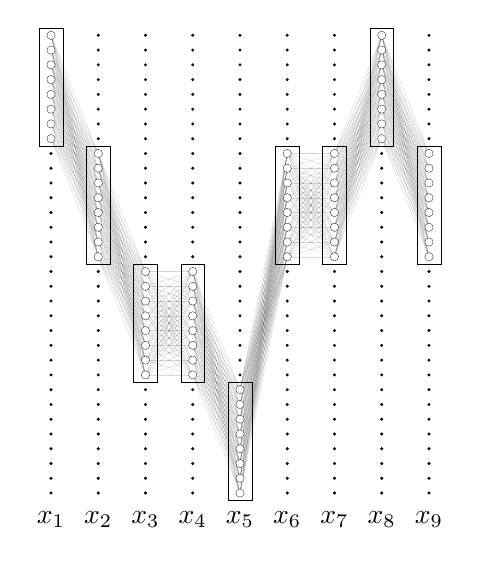
\begin{tikzpicture}%
\path[draw,line width=0.1pt,opacity=0.15,fill=black] (0.6,4.5) -- (1.2,3.0);%
\path[draw,line width=0.1pt,opacity=0.15,fill=black] (0.6,4.5) -- (1.2,3.1875);%
\path[draw,line width=0.1pt,opacity=0.15,fill=black] (0.6,4.5) -- (1.2,3.375);%
\path[draw,line width=0.1pt,opacity=0.15,fill=black] (0.6,4.5) -- (1.2,3.5625);%
\path[draw,line width=0.1pt,opacity=0.15,fill=black] (0.6,4.5) -- (1.2,3.75);%
\path[draw,line width=0.1pt,opacity=0.15,fill=black] (0.6,4.5) -- (1.2,3.9375);%
\path[draw,line width=0.1pt,opacity=0.15,fill=black] (0.6,4.5) -- (1.2,4.125);%
\path[draw,line width=0.1pt,opacity=0.15,fill=black] (0.6,4.5) -- (1.2,4.3125);%
\path[draw,line width=0.1pt,opacity=0.15,fill=black] (0.6,4.6875) -- (1.2,3.0);%
\path[draw,line width=0.1pt,opacity=0.15,fill=black] (0.6,4.6875) -- (1.2,3.1875);%
\path[draw,line width=0.1pt,opacity=0.15,fill=black] (0.6,4.6875) -- (1.2,3.375);%
\path[draw,line width=0.1pt,opacity=0.15,fill=black] (0.6,4.6875) -- (1.2,3.5625);%
\path[draw,line width=0.1pt,opacity=0.15,fill=black] (0.6,4.6875) -- (1.2,3.75);%
\path[draw,line width=0.1pt,opacity=0.15,fill=black] (0.6,4.6875) -- (1.2,3.9375);%
\path[draw,line width=0.1pt,opacity=0.15,fill=black] (0.6,4.6875) -- (1.2,4.125);%
\path[draw,line width=0.1pt,opacity=0.15,fill=black] (0.6,4.6875) -- (1.2,4.3125);%
\path[draw,line width=0.1pt,opacity=0.15,fill=black] (0.6,4.875) -- (1.2,3.0);%
\path[draw,line width=0.1pt,opacity=0.15,fill=black] (0.6,4.875) -- (1.2,3.1875);%
\path[draw,line width=0.1pt,opacity=0.15,fill=black] (0.6,4.875) -- (1.2,3.375);%
\path[draw,line width=0.1pt,opacity=0.15,fill=black] (0.6,4.875) -- (1.2,3.5625);%
\path[draw,line width=0.1pt,opacity=0.15,fill=black] (0.6,4.875) -- (1.2,3.75);%
\path[draw,line width=0.1pt,opacity=0.15,fill=black] (0.6,4.875) -- (1.2,3.9375);%
\path[draw,line width=0.1pt,opacity=0.15,fill=black] (0.6,4.875) -- (1.2,4.125);%
\path[draw,line width=0.1pt,opacity=0.15,fill=black] (0.6,4.875) -- (1.2,4.3125);%
\path[draw,line width=0.1pt,opacity=0.15,fill=black] (0.6,5.0625) -- (1.2,3.0);%
\path[draw,line width=0.1pt,opacity=0.15,fill=black] (0.6,5.0625) -- (1.2,3.1875);%
\path[draw,line width=0.1pt,opacity=0.15,fill=black] (0.6,5.0625) -- (1.2,3.375);%
\path[draw,line width=0.1pt,opacity=0.15,fill=black] (0.6,5.0625) -- (1.2,3.5625);%
\path[draw,line width=0.1pt,opacity=0.15,fill=black] (0.6,5.0625) -- (1.2,3.75);%
\path[draw,line width=0.1pt,opacity=0.15,fill=black] (0.6,5.0625) -- (1.2,3.9375);%
\path[draw,line width=0.1pt,opacity=0.15,fill=black] (0.6,5.0625) -- (1.2,4.125);%
\path[draw,line width=0.1pt,opacity=0.15,fill=black] (0.6,5.0625) -- (1.2,4.3125);%
\path[draw,line width=0.1pt,opacity=0.15,fill=black] (0.6,5.25) -- (1.2,3.0);%
\path[draw,line width=0.1pt,opacity=0.15,fill=black] (0.6,5.25) -- (1.2,3.1875);%
\path[draw,line width=0.1pt,opacity=0.15,fill=black] (0.6,5.25) -- (1.2,3.375);%
\path[draw,line width=0.1pt,opacity=0.15,fill=black] (0.6,5.25) -- (1.2,3.5625);%
\path[draw,line width=0.1pt,opacity=0.15,fill=black] (0.6,5.25) -- (1.2,3.75);%
\path[draw,line width=0.1pt,opacity=0.15,fill=black] (0.6,5.25) -- (1.2,3.9375);%
\path[draw,line width=0.1pt,opacity=0.15,fill=black] (0.6,5.25) -- (1.2,4.125);%
\path[draw,line width=0.1pt,opacity=0.15,fill=black] (0.6,5.25) -- (1.2,4.3125);%
\path[draw,line width=0.1pt,opacity=0.15,fill=black] (0.6,5.4375) -- (1.2,3.0);%
\path[draw,line width=0.1pt,opacity=0.15,fill=black] (0.6,5.4375) -- (1.2,3.1875);%
\path[draw,line width=0.1pt,opacity=0.15,fill=black] (0.6,5.4375) -- (1.2,3.375);%
\path[draw,line width=0.1pt,opacity=0.15,fill=black] (0.6,5.4375) -- (1.2,3.5625);%
\path[draw,line width=0.1pt,opacity=0.15,fill=black] (0.6,5.4375) -- (1.2,3.75);%
\path[draw,line width=0.1pt,opacity=0.15,fill=black] (0.6,5.4375) -- (1.2,3.9375);%
\path[draw,line width=0.1pt,opacity=0.15,fill=black] (0.6,5.4375) -- (1.2,4.125);%
\path[draw,line width=0.1pt,opacity=0.15,fill=black] (0.6,5.4375) -- (1.2,4.3125);%
\path[draw,line width=0.1pt,opacity=0.15,fill=black] (0.6,5.625) -- (1.2,3.0);%
\path[draw,line width=0.1pt,opacity=0.15,fill=black] (0.6,5.625) -- (1.2,3.1875);%
\path[draw,line width=0.1pt,opacity=0.15,fill=black] (0.6,5.625) -- (1.2,3.375);%
\path[draw,line width=0.1pt,opacity=0.15,fill=black] (0.6,5.625) -- (1.2,3.5625);%
\path[draw,line width=0.1pt,opacity=0.15,fill=black] (0.6,5.625) -- (1.2,3.75);%
\path[draw,line width=0.1pt,opacity=0.15,fill=black] (0.6,5.625) -- (1.2,3.9375);%
\path[draw,line width=0.1pt,opacity=0.15,fill=black] (0.6,5.625) -- (1.2,4.125);%
\path[draw,line width=0.1pt,opacity=0.15,fill=black] (0.6,5.625) -- (1.2,4.3125);%
\path[draw,line width=0.1pt,opacity=0.15,fill=black] (0.6,5.8125) -- (1.2,3.0);%
\path[draw,line width=0.1pt,opacity=0.15,fill=black] (0.6,5.8125) -- (1.2,3.1875);%
\path[draw,line width=0.1pt,opacity=0.15,fill=black] (0.6,5.8125) -- (1.2,3.375);%
\path[draw,line width=0.1pt,opacity=0.15,fill=black] (0.6,5.8125) -- (1.2,3.5625);%
\path[draw,line width=0.1pt,opacity=0.15,fill=black] (0.6,5.8125) -- (1.2,3.75);%
\path[draw,line width=0.1pt,opacity=0.15,fill=black] (0.6,5.8125) -- (1.2,3.9375);%
\path[draw,line width=0.1pt,opacity=0.15,fill=black] (0.6,5.8125) -- (1.2,4.125);%
\path[draw,line width=0.1pt,opacity=0.15,fill=black] (0.6,5.8125) -- (1.2,4.3125);%
\path[draw,line width=0.1pt,opacity=0.15,fill=black] (1.2,3.0) -- (1.8,1.5);%
\path[draw,line width=0.1pt,opacity=0.15,fill=black] (1.2,3.0) -- (1.8,1.6875);%
\path[draw,line width=0.1pt,opacity=0.15,fill=black] (1.2,3.0) -- (1.8,1.875);%
\path[draw,line width=0.1pt,opacity=0.15,fill=black] (1.2,3.0) -- (1.8,2.0625);%
\path[draw,line width=0.1pt,opacity=0.15,fill=black] (1.2,3.0) -- (1.8,2.25);%
\path[draw,line width=0.1pt,opacity=0.15,fill=black] (1.2,3.0) -- (1.8,2.4375);%
\path[draw,line width=0.1pt,opacity=0.15,fill=black] (1.2,3.0) -- (1.8,2.625);%
\path[draw,line width=0.1pt,opacity=0.15,fill=black] (1.2,3.0) -- (1.8,2.8125);%
\path[draw,line width=0.1pt,opacity=0.15,fill=black] (1.2,3.1875) -- (1.8,1.5);%
\path[draw,line width=0.1pt,opacity=0.15,fill=black] (1.2,3.1875) -- (1.8,1.6875);%
\path[draw,line width=0.1pt,opacity=0.15,fill=black] (1.2,3.1875) -- (1.8,1.875);%
\path[draw,line width=0.1pt,opacity=0.15,fill=black] (1.2,3.1875) -- (1.8,2.0625);%
\path[draw,line width=0.1pt,opacity=0.15,fill=black] (1.2,3.1875) -- (1.8,2.25);%
\path[draw,line width=0.1pt,opacity=0.15,fill=black] (1.2,3.1875) -- (1.8,2.4375);%
\path[draw,line width=0.1pt,opacity=0.15,fill=black] (1.2,3.1875) -- (1.8,2.625);%
\path[draw,line width=0.1pt,opacity=0.15,fill=black] (1.2,3.1875) -- (1.8,2.8125);%
\path[draw,line width=0.1pt,opacity=0.15,fill=black] (1.2,3.375) -- (1.8,1.5);%
\path[draw,line width=0.1pt,opacity=0.15,fill=black] (1.2,3.375) -- (1.8,1.6875);%
\path[draw,line width=0.1pt,opacity=0.15,fill=black] (1.2,3.375) -- (1.8,1.875);%
\path[draw,line width=0.1pt,opacity=0.15,fill=black] (1.2,3.375) -- (1.8,2.0625);%
\path[draw,line width=0.1pt,opacity=0.15,fill=black] (1.2,3.375) -- (1.8,2.25);%
\path[draw,line width=0.1pt,opacity=0.15,fill=black] (1.2,3.375) -- (1.8,2.4375);%
\path[draw,line width=0.1pt,opacity=0.15,fill=black] (1.2,3.375) -- (1.8,2.625);%
\path[draw,line width=0.1pt,opacity=0.15,fill=black] (1.2,3.375) -- (1.8,2.8125);%
\path[draw,line width=0.1pt,opacity=0.15,fill=black] (1.2,3.5625) -- (1.8,1.5);%
\path[draw,line width=0.1pt,opacity=0.15,fill=black] (1.2,3.5625) -- (1.8,1.6875);%
\path[draw,line width=0.1pt,opacity=0.15,fill=black] (1.2,3.5625) -- (1.8,1.875);%
\path[draw,line width=0.1pt,opacity=0.15,fill=black] (1.2,3.5625) -- (1.8,2.0625);%
\path[draw,line width=0.1pt,opacity=0.15,fill=black] (1.2,3.5625) -- (1.8,2.25);%
\path[draw,line width=0.1pt,opacity=0.15,fill=black] (1.2,3.5625) -- (1.8,2.4375);%
\path[draw,line width=0.1pt,opacity=0.15,fill=black] (1.2,3.5625) -- (1.8,2.625);%
\path[draw,line width=0.1pt,opacity=0.15,fill=black] (1.2,3.5625) -- (1.8,2.8125);%
\path[draw,line width=0.1pt,opacity=0.15,fill=black] (1.2,3.75) -- (1.8,1.5);%
\path[draw,line width=0.1pt,opacity=0.15,fill=black] (1.2,3.75) -- (1.8,1.6875);%
\path[draw,line width=0.1pt,opacity=0.15,fill=black] (1.2,3.75) -- (1.8,1.875);%
\path[draw,line width=0.1pt,opacity=0.15,fill=black] (1.2,3.75) -- (1.8,2.0625);%
\path[draw,line width=0.1pt,opacity=0.15,fill=black] (1.2,3.75) -- (1.8,2.25);%
\path[draw,line width=0.1pt,opacity=0.15,fill=black] (1.2,3.75) -- (1.8,2.4375);%
\path[draw,line width=0.1pt,opacity=0.15,fill=black] (1.2,3.75) -- (1.8,2.625);%
\path[draw,line width=0.1pt,opacity=0.15,fill=black] (1.2,3.75) -- (1.8,2.8125);%
\path[draw,line width=0.1pt,opacity=0.15,fill=black] (1.2,3.9375) -- (1.8,1.5);%
\path[draw,line width=0.1pt,opacity=0.15,fill=black] (1.2,3.9375) -- (1.8,1.6875);%
\path[draw,line width=0.1pt,opacity=0.15,fill=black] (1.2,3.9375) -- (1.8,1.875);%
\path[draw,line width=0.1pt,opacity=0.15,fill=black] (1.2,3.9375) -- (1.8,2.0625);%
\path[draw,line width=0.1pt,opacity=0.15,fill=black] (1.2,3.9375) -- (1.8,2.25);%
\path[draw,line width=0.1pt,opacity=0.15,fill=black] (1.2,3.9375) -- (1.8,2.4375);%
\path[draw,line width=0.1pt,opacity=0.15,fill=black] (1.2,3.9375) -- (1.8,2.625);%
\path[draw,line width=0.1pt,opacity=0.15,fill=black] (1.2,3.9375) -- (1.8,2.8125);%
\path[draw,line width=0.1pt,opacity=0.15,fill=black] (1.2,4.125) -- (1.8,1.5);%
\path[draw,line width=0.1pt,opacity=0.15,fill=black] (1.2,4.125) -- (1.8,1.6875);%
\path[draw,line width=0.1pt,opacity=0.15,fill=black] (1.2,4.125) -- (1.8,1.875);%
\path[draw,line width=0.1pt,opacity=0.15,fill=black] (1.2,4.125) -- (1.8,2.0625);%
\path[draw,line width=0.1pt,opacity=0.15,fill=black] (1.2,4.125) -- (1.8,2.25);%
\path[draw,line width=0.1pt,opacity=0.15,fill=black] (1.2,4.125) -- (1.8,2.4375);%
\path[draw,line width=0.1pt,opacity=0.15,fill=black] (1.2,4.125) -- (1.8,2.625);%
\path[draw,line width=0.1pt,opacity=0.15,fill=black] (1.2,4.125) -- (1.8,2.8125);%
\path[draw,line width=0.1pt,opacity=0.15,fill=black] (1.2,4.3125) -- (1.8,1.5);%
\path[draw,line width=0.1pt,opacity=0.15,fill=black] (1.2,4.3125) -- (1.8,1.6875);%
\path[draw,line width=0.1pt,opacity=0.15,fill=black] (1.2,4.3125) -- (1.8,1.875);%
\path[draw,line width=0.1pt,opacity=0.15,fill=black] (1.2,4.3125) -- (1.8,2.0625);%
\path[draw,line width=0.1pt,opacity=0.15,fill=black] (1.2,4.3125) -- (1.8,2.25);%
\path[draw,line width=0.1pt,opacity=0.15,fill=black] (1.2,4.3125) -- (1.8,2.4375);%
\path[draw,line width=0.1pt,opacity=0.15,fill=black] (1.2,4.3125) -- (1.8,2.625);%
\path[draw,line width=0.1pt,opacity=0.15,fill=black] (1.2,4.3125) -- (1.8,2.8125);%
\path[draw,line width=0.1pt,opacity=0.15,fill=black] (1.8,1.5) -- (2.4,1.5);%
\path[draw,line width=0.1pt,opacity=0.15,fill=black] (1.8,1.5) -- (2.4,1.6875);%
\path[draw,line width=0.1pt,opacity=0.15,fill=black] (1.8,1.5) -- (2.4,1.875);%
\path[draw,line width=0.1pt,opacity=0.15,fill=black] (1.8,1.5) -- (2.4,2.0625);%
\path[draw,line width=0.1pt,opacity=0.15,fill=black] (1.8,1.5) -- (2.4,2.25);%
\path[draw,line width=0.1pt,opacity=0.15,fill=black] (1.8,1.5) -- (2.4,2.4375);%
\path[draw,line width=0.1pt,opacity=0.15,fill=black] (1.8,1.5) -- (2.4,2.625);%
\path[draw,line width=0.1pt,opacity=0.15,fill=black] (1.8,1.5) -- (2.4,2.8125);%
\path[draw,line width=0.1pt,opacity=0.15,fill=black] (1.8,1.6875) -- (2.4,1.5);%
\path[draw,line width=0.1pt,opacity=0.15,fill=black] (1.8,1.6875) -- (2.4,1.6875);%
\path[draw,line width=0.1pt,opacity=0.15,fill=black] (1.8,1.6875) -- (2.4,1.875);%
\path[draw,line width=0.1pt,opacity=0.15,fill=black] (1.8,1.6875) -- (2.4,2.0625);%
\path[draw,line width=0.1pt,opacity=0.15,fill=black] (1.8,1.6875) -- (2.4,2.25);%
\path[draw,line width=0.1pt,opacity=0.15,fill=black] (1.8,1.6875) -- (2.4,2.4375);%
\path[draw,line width=0.1pt,opacity=0.15,fill=black] (1.8,1.6875) -- (2.4,2.625);%
\path[draw,line width=0.1pt,opacity=0.15,fill=black] (1.8,1.6875) -- (2.4,2.8125);%
\path[draw,line width=0.1pt,opacity=0.15,fill=black] (1.8,1.875) -- (2.4,1.5);%
\path[draw,line width=0.1pt,opacity=0.15,fill=black] (1.8,1.875) -- (2.4,1.6875);%
\path[draw,line width=0.1pt,opacity=0.15,fill=black] (1.8,1.875) -- (2.4,1.875);%
\path[draw,line width=0.1pt,opacity=0.15,fill=black] (1.8,1.875) -- (2.4,2.0625);%
\path[draw,line width=0.1pt,opacity=0.15,fill=black] (1.8,1.875) -- (2.4,2.25);%
\path[draw,line width=0.1pt,opacity=0.15,fill=black] (1.8,1.875) -- (2.4,2.4375);%
\path[draw,line width=0.1pt,opacity=0.15,fill=black] (1.8,1.875) -- (2.4,2.625);%
\path[draw,line width=0.1pt,opacity=0.15,fill=black] (1.8,1.875) -- (2.4,2.8125);%
\path[draw,line width=0.1pt,opacity=0.15,fill=black] (1.8,2.0625) -- (2.4,1.5);%
\path[draw,line width=0.1pt,opacity=0.15,fill=black] (1.8,2.0625) -- (2.4,1.6875);%
\path[draw,line width=0.1pt,opacity=0.15,fill=black] (1.8,2.0625) -- (2.4,1.875);%
\path[draw,line width=0.1pt,opacity=0.15,fill=black] (1.8,2.0625) -- (2.4,2.0625);%
\path[draw,line width=0.1pt,opacity=0.15,fill=black] (1.8,2.0625) -- (2.4,2.25);%
\path[draw,line width=0.1pt,opacity=0.15,fill=black] (1.8,2.0625) -- (2.4,2.4375);%
\path[draw,line width=0.1pt,opacity=0.15,fill=black] (1.8,2.0625) -- (2.4,2.625);%
\path[draw,line width=0.1pt,opacity=0.15,fill=black] (1.8,2.0625) -- (2.4,2.8125);%
\path[draw,line width=0.1pt,opacity=0.15,fill=black] (1.8,2.25) -- (2.4,1.5);%
\path[draw,line width=0.1pt,opacity=0.15,fill=black] (1.8,2.25) -- (2.4,1.6875);%
\path[draw,line width=0.1pt,opacity=0.15,fill=black] (1.8,2.25) -- (2.4,1.875);%
\path[draw,line width=0.1pt,opacity=0.15,fill=black] (1.8,2.25) -- (2.4,2.0625);%
\path[draw,line width=0.1pt,opacity=0.15,fill=black] (1.8,2.25) -- (2.4,2.25);%
\path[draw,line width=0.1pt,opacity=0.15,fill=black] (1.8,2.25) -- (2.4,2.4375);%
\path[draw,line width=0.1pt,opacity=0.15,fill=black] (1.8,2.25) -- (2.4,2.625);%
\path[draw,line width=0.1pt,opacity=0.15,fill=black] (1.8,2.25) -- (2.4,2.8125);%
\path[draw,line width=0.1pt,opacity=0.15,fill=black] (1.8,2.4375) -- (2.4,1.5);%
\path[draw,line width=0.1pt,opacity=0.15,fill=black] (1.8,2.4375) -- (2.4,1.6875);%
\path[draw,line width=0.1pt,opacity=0.15,fill=black] (1.8,2.4375) -- (2.4,1.875);%
\path[draw,line width=0.1pt,opacity=0.15,fill=black] (1.8,2.4375) -- (2.4,2.0625);%
\path[draw,line width=0.1pt,opacity=0.15,fill=black] (1.8,2.4375) -- (2.4,2.25);%
\path[draw,line width=0.1pt,opacity=0.15,fill=black] (1.8,2.4375) -- (2.4,2.4375);%
\path[draw,line width=0.1pt,opacity=0.15,fill=black] (1.8,2.4375) -- (2.4,2.625);%
\path[draw,line width=0.1pt,opacity=0.15,fill=black] (1.8,2.4375) -- (2.4,2.8125);%
\path[draw,line width=0.1pt,opacity=0.15,fill=black] (1.8,2.625) -- (2.4,1.5);%
\path[draw,line width=0.1pt,opacity=0.15,fill=black] (1.8,2.625) -- (2.4,1.6875);%
\path[draw,line width=0.1pt,opacity=0.15,fill=black] (1.8,2.625) -- (2.4,1.875);%
\path[draw,line width=0.1pt,opacity=0.15,fill=black] (1.8,2.625) -- (2.4,2.0625);%
\path[draw,line width=0.1pt,opacity=0.15,fill=black] (1.8,2.625) -- (2.4,2.25);%
\path[draw,line width=0.1pt,opacity=0.15,fill=black] (1.8,2.625) -- (2.4,2.4375);%
\path[draw,line width=0.1pt,opacity=0.15,fill=black] (1.8,2.625) -- (2.4,2.625);%
\path[draw,line width=0.1pt,opacity=0.15,fill=black] (1.8,2.625) -- (2.4,2.8125);%
\path[draw,line width=0.1pt,opacity=0.15,fill=black] (1.8,2.8125) -- (2.4,1.5);%
\path[draw,line width=0.1pt,opacity=0.15,fill=black] (1.8,2.8125) -- (2.4,1.6875);%
\path[draw,line width=0.1pt,opacity=0.15,fill=black] (1.8,2.8125) -- (2.4,1.875);%
\path[draw,line width=0.1pt,opacity=0.15,fill=black] (1.8,2.8125) -- (2.4,2.0625);%
\path[draw,line width=0.1pt,opacity=0.15,fill=black] (1.8,2.8125) -- (2.4,2.25);%
\path[draw,line width=0.1pt,opacity=0.15,fill=black] (1.8,2.8125) -- (2.4,2.4375);%
\path[draw,line width=0.1pt,opacity=0.15,fill=black] (1.8,2.8125) -- (2.4,2.625);%
\path[draw,line width=0.1pt,opacity=0.15,fill=black] (1.8,2.8125) -- (2.4,2.8125);%
\path[draw,line width=0.1pt,opacity=0.15,fill=black] (2.4,1.5) -- (3.0,0.0);%
\path[draw,line width=0.1pt,opacity=0.15,fill=black] (2.4,1.5) -- (3.0,0.1875);%
\path[draw,line width=0.1pt,opacity=0.15,fill=black] (2.4,1.5) -- (3.0,0.375);%
\path[draw,line width=0.1pt,opacity=0.15,fill=black] (2.4,1.5) -- (3.0,0.5625);%
\path[draw,line width=0.1pt,opacity=0.15,fill=black] (2.4,1.5) -- (3.0,0.75);%
\path[draw,line width=0.1pt,opacity=0.15,fill=black] (2.4,1.5) -- (3.0,0.9375);%
\path[draw,line width=0.1pt,opacity=0.15,fill=black] (2.4,1.5) -- (3.0,1.125);%
\path[draw,line width=0.1pt,opacity=0.15,fill=black] (2.4,1.5) -- (3.0,1.3125);%
\path[draw,line width=0.1pt,opacity=0.15,fill=black] (2.4,1.6875) -- (3.0,0.0);%
\path[draw,line width=0.1pt,opacity=0.15,fill=black] (2.4,1.6875) -- (3.0,0.1875);%
\path[draw,line width=0.1pt,opacity=0.15,fill=black] (2.4,1.6875) -- (3.0,0.375);%
\path[draw,line width=0.1pt,opacity=0.15,fill=black] (2.4,1.6875) -- (3.0,0.5625);%
\path[draw,line width=0.1pt,opacity=0.15,fill=black] (2.4,1.6875) -- (3.0,0.75);%
\path[draw,line width=0.1pt,opacity=0.15,fill=black] (2.4,1.6875) -- (3.0,0.9375);%
\path[draw,line width=0.1pt,opacity=0.15,fill=black] (2.4,1.6875) -- (3.0,1.125);%
\path[draw,line width=0.1pt,opacity=0.15,fill=black] (2.4,1.6875) -- (3.0,1.3125);%
\path[draw,line width=0.1pt,opacity=0.15,fill=black] (2.4,1.875) -- (3.0,0.0);%
\path[draw,line width=0.1pt,opacity=0.15,fill=black] (2.4,1.875) -- (3.0,0.1875);%
\path[draw,line width=0.1pt,opacity=0.15,fill=black] (2.4,1.875) -- (3.0,0.375);%
\path[draw,line width=0.1pt,opacity=0.15,fill=black] (2.4,1.875) -- (3.0,0.5625);%
\path[draw,line width=0.1pt,opacity=0.15,fill=black] (2.4,1.875) -- (3.0,0.75);%
\path[draw,line width=0.1pt,opacity=0.15,fill=black] (2.4,1.875) -- (3.0,0.9375);%
\path[draw,line width=0.1pt,opacity=0.15,fill=black] (2.4,1.875) -- (3.0,1.125);%
\path[draw,line width=0.1pt,opacity=0.15,fill=black] (2.4,1.875) -- (3.0,1.3125);%
\path[draw,line width=0.1pt,opacity=0.15,fill=black] (2.4,2.0625) -- (3.0,0.0);%
\path[draw,line width=0.1pt,opacity=0.15,fill=black] (2.4,2.0625) -- (3.0,0.1875);%
\path[draw,line width=0.1pt,opacity=0.15,fill=black] (2.4,2.0625) -- (3.0,0.375);%
\path[draw,line width=0.1pt,opacity=0.15,fill=black] (2.4,2.0625) -- (3.0,0.5625);%
\path[draw,line width=0.1pt,opacity=0.15,fill=black] (2.4,2.0625) -- (3.0,0.75);%
\path[draw,line width=0.1pt,opacity=0.15,fill=black] (2.4,2.0625) -- (3.0,0.9375);%
\path[draw,line width=0.1pt,opacity=0.15,fill=black] (2.4,2.0625) -- (3.0,1.125);%
\path[draw,line width=0.1pt,opacity=0.15,fill=black] (2.4,2.0625) -- (3.0,1.3125);%
\path[draw,line width=0.1pt,opacity=0.15,fill=black] (2.4,2.25) -- (3.0,0.0);%
\path[draw,line width=0.1pt,opacity=0.15,fill=black] (2.4,2.25) -- (3.0,0.1875);%
\path[draw,line width=0.1pt,opacity=0.15,fill=black] (2.4,2.25) -- (3.0,0.375);%
\path[draw,line width=0.1pt,opacity=0.15,fill=black] (2.4,2.25) -- (3.0,0.5625);%
\path[draw,line width=0.1pt,opacity=0.15,fill=black] (2.4,2.25) -- (3.0,0.75);%
\path[draw,line width=0.1pt,opacity=0.15,fill=black] (2.4,2.25) -- (3.0,0.9375);%
\path[draw,line width=0.1pt,opacity=0.15,fill=black] (2.4,2.25) -- (3.0,1.125);%
\path[draw,line width=0.1pt,opacity=0.15,fill=black] (2.4,2.25) -- (3.0,1.3125);%
\path[draw,line width=0.1pt,opacity=0.15,fill=black] (2.4,2.4375) -- (3.0,0.0);%
\path[draw,line width=0.1pt,opacity=0.15,fill=black] (2.4,2.4375) -- (3.0,0.1875);%
\path[draw,line width=0.1pt,opacity=0.15,fill=black] (2.4,2.4375) -- (3.0,0.375);%
\path[draw,line width=0.1pt,opacity=0.15,fill=black] (2.4,2.4375) -- (3.0,0.5625);%
\path[draw,line width=0.1pt,opacity=0.15,fill=black] (2.4,2.4375) -- (3.0,0.75);%
\path[draw,line width=0.1pt,opacity=0.15,fill=black] (2.4,2.4375) -- (3.0,0.9375);%
\path[draw,line width=0.1pt,opacity=0.15,fill=black] (2.4,2.4375) -- (3.0,1.125);%
\path[draw,line width=0.1pt,opacity=0.15,fill=black] (2.4,2.4375) -- (3.0,1.3125);%
\path[draw,line width=0.1pt,opacity=0.15,fill=black] (2.4,2.625) -- (3.0,0.0);%
\path[draw,line width=0.1pt,opacity=0.15,fill=black] (2.4,2.625) -- (3.0,0.1875);%
\path[draw,line width=0.1pt,opacity=0.15,fill=black] (2.4,2.625) -- (3.0,0.375);%
\path[draw,line width=0.1pt,opacity=0.15,fill=black] (2.4,2.625) -- (3.0,0.5625);%
\path[draw,line width=0.1pt,opacity=0.15,fill=black] (2.4,2.625) -- (3.0,0.75);%
\path[draw,line width=0.1pt,opacity=0.15,fill=black] (2.4,2.625) -- (3.0,0.9375);%
\path[draw,line width=0.1pt,opacity=0.15,fill=black] (2.4,2.625) -- (3.0,1.125);%
\path[draw,line width=0.1pt,opacity=0.15,fill=black] (2.4,2.625) -- (3.0,1.3125);%
\path[draw,line width=0.1pt,opacity=0.15,fill=black] (2.4,2.8125) -- (3.0,0.0);%
\path[draw,line width=0.1pt,opacity=0.15,fill=black] (2.4,2.8125) -- (3.0,0.1875);%
\path[draw,line width=0.1pt,opacity=0.15,fill=black] (2.4,2.8125) -- (3.0,0.375);%
\path[draw,line width=0.1pt,opacity=0.15,fill=black] (2.4,2.8125) -- (3.0,0.5625);%
\path[draw,line width=0.1pt,opacity=0.15,fill=black] (2.4,2.8125) -- (3.0,0.75);%
\path[draw,line width=0.1pt,opacity=0.15,fill=black] (2.4,2.8125) -- (3.0,0.9375);%
\path[draw,line width=0.1pt,opacity=0.15,fill=black] (2.4,2.8125) -- (3.0,1.125);%
\path[draw,line width=0.1pt,opacity=0.15,fill=black] (2.4,2.8125) -- (3.0,1.3125);%
\path[draw,line width=0.1pt,opacity=0.15,fill=black] (3.0,0.0) -- (3.6,3.0);%
\path[draw,line width=0.1pt,opacity=0.15,fill=black] (3.0,0.0) -- (3.6,3.1875);%
\path[draw,line width=0.1pt,opacity=0.15,fill=black] (3.0,0.0) -- (3.6,3.375);%
\path[draw,line width=0.1pt,opacity=0.15,fill=black] (3.0,0.0) -- (3.6,3.5625);%
\path[draw,line width=0.1pt,opacity=0.15,fill=black] (3.0,0.0) -- (3.6,3.75);%
\path[draw,line width=0.1pt,opacity=0.15,fill=black] (3.0,0.0) -- (3.6,3.9375);%
\path[draw,line width=0.1pt,opacity=0.15,fill=black] (3.0,0.0) -- (3.6,4.125);%
\path[draw,line width=0.1pt,opacity=0.15,fill=black] (3.0,0.0) -- (3.6,4.3125);%
\path[draw,line width=0.1pt,opacity=0.15,fill=black] (3.0,0.1875) -- (3.6,3.0);%
\path[draw,line width=0.1pt,opacity=0.15,fill=black] (3.0,0.1875) -- (3.6,3.1875);%
\path[draw,line width=0.1pt,opacity=0.15,fill=black] (3.0,0.1875) -- (3.6,3.375);%
\path[draw,line width=0.1pt,opacity=0.15,fill=black] (3.0,0.1875) -- (3.6,3.5625);%
\path[draw,line width=0.1pt,opacity=0.15,fill=black] (3.0,0.1875) -- (3.6,3.75);%
\path[draw,line width=0.1pt,opacity=0.15,fill=black] (3.0,0.1875) -- (3.6,3.9375);%
\path[draw,line width=0.1pt,opacity=0.15,fill=black] (3.0,0.1875) -- (3.6,4.125);%
\path[draw,line width=0.1pt,opacity=0.15,fill=black] (3.0,0.1875) -- (3.6,4.3125);%
\path[draw,line width=0.1pt,opacity=0.15,fill=black] (3.0,0.375) -- (3.6,3.0);%
\path[draw,line width=0.1pt,opacity=0.15,fill=black] (3.0,0.375) -- (3.6,3.1875);%
\path[draw,line width=0.1pt,opacity=0.15,fill=black] (3.0,0.375) -- (3.6,3.375);%
\path[draw,line width=0.1pt,opacity=0.15,fill=black] (3.0,0.375) -- (3.6,3.5625);%
\path[draw,line width=0.1pt,opacity=0.15,fill=black] (3.0,0.375) -- (3.6,3.75);%
\path[draw,line width=0.1pt,opacity=0.15,fill=black] (3.0,0.375) -- (3.6,3.9375);%
\path[draw,line width=0.1pt,opacity=0.15,fill=black] (3.0,0.375) -- (3.6,4.125);%
\path[draw,line width=0.1pt,opacity=0.15,fill=black] (3.0,0.375) -- (3.6,4.3125);%
\path[draw,line width=0.1pt,opacity=0.15,fill=black] (3.0,0.5625) -- (3.6,3.0);%
\path[draw,line width=0.1pt,opacity=0.15,fill=black] (3.0,0.5625) -- (3.6,3.1875);%
\path[draw,line width=0.1pt,opacity=0.15,fill=black] (3.0,0.5625) -- (3.6,3.375);%
\path[draw,line width=0.1pt,opacity=0.15,fill=black] (3.0,0.5625) -- (3.6,3.5625);%
\path[draw,line width=0.1pt,opacity=0.15,fill=black] (3.0,0.5625) -- (3.6,3.75);%
\path[draw,line width=0.1pt,opacity=0.15,fill=black] (3.0,0.5625) -- (3.6,3.9375);%
\path[draw,line width=0.1pt,opacity=0.15,fill=black] (3.0,0.5625) -- (3.6,4.125);%
\path[draw,line width=0.1pt,opacity=0.15,fill=black] (3.0,0.5625) -- (3.6,4.3125);%
\path[draw,line width=0.1pt,opacity=0.15,fill=black] (3.0,0.75) -- (3.6,3.0);%
\path[draw,line width=0.1pt,opacity=0.15,fill=black] (3.0,0.75) -- (3.6,3.1875);%
\path[draw,line width=0.1pt,opacity=0.15,fill=black] (3.0,0.75) -- (3.6,3.375);%
\path[draw,line width=0.1pt,opacity=0.15,fill=black] (3.0,0.75) -- (3.6,3.5625);%
\path[draw,line width=0.1pt,opacity=0.15,fill=black] (3.0,0.75) -- (3.6,3.75);%
\path[draw,line width=0.1pt,opacity=0.15,fill=black] (3.0,0.75) -- (3.6,3.9375);%
\path[draw,line width=0.1pt,opacity=0.15,fill=black] (3.0,0.75) -- (3.6,4.125);%
\path[draw,line width=0.1pt,opacity=0.15,fill=black] (3.0,0.75) -- (3.6,4.3125);%
\path[draw,line width=0.1pt,opacity=0.15,fill=black] (3.0,0.9375) -- (3.6,3.0);%
\path[draw,line width=0.1pt,opacity=0.15,fill=black] (3.0,0.9375) -- (3.6,3.1875);%
\path[draw,line width=0.1pt,opacity=0.15,fill=black] (3.0,0.9375) -- (3.6,3.375);%
\path[draw,line width=0.1pt,opacity=0.15,fill=black] (3.0,0.9375) -- (3.6,3.5625);%
\path[draw,line width=0.1pt,opacity=0.15,fill=black] (3.0,0.9375) -- (3.6,3.75);%
\path[draw,line width=0.1pt,opacity=0.15,fill=black] (3.0,0.9375) -- (3.6,3.9375);%
\path[draw,line width=0.1pt,opacity=0.15,fill=black] (3.0,0.9375) -- (3.6,4.125);%
\path[draw,line width=0.1pt,opacity=0.15,fill=black] (3.0,0.9375) -- (3.6,4.3125);%
\path[draw,line width=0.1pt,opacity=0.15,fill=black] (3.0,1.125) -- (3.6,3.0);%
\path[draw,line width=0.1pt,opacity=0.15,fill=black] (3.0,1.125) -- (3.6,3.1875);%
\path[draw,line width=0.1pt,opacity=0.15,fill=black] (3.0,1.125) -- (3.6,3.375);%
\path[draw,line width=0.1pt,opacity=0.15,fill=black] (3.0,1.125) -- (3.6,3.5625);%
\path[draw,line width=0.1pt,opacity=0.15,fill=black] (3.0,1.125) -- (3.6,3.75);%
\path[draw,line width=0.1pt,opacity=0.15,fill=black] (3.0,1.125) -- (3.6,3.9375);%
\path[draw,line width=0.1pt,opacity=0.15,fill=black] (3.0,1.125) -- (3.6,4.125);%
\path[draw,line width=0.1pt,opacity=0.15,fill=black] (3.0,1.125) -- (3.6,4.3125);%
\path[draw,line width=0.1pt,opacity=0.15,fill=black] (3.0,1.3125) -- (3.6,3.0);%
\path[draw,line width=0.1pt,opacity=0.15,fill=black] (3.0,1.3125) -- (3.6,3.1875);%
\path[draw,line width=0.1pt,opacity=0.15,fill=black] (3.0,1.3125) -- (3.6,3.375);%
\path[draw,line width=0.1pt,opacity=0.15,fill=black] (3.0,1.3125) -- (3.6,3.5625);%
\path[draw,line width=0.1pt,opacity=0.15,fill=black] (3.0,1.3125) -- (3.6,3.75);%
\path[draw,line width=0.1pt,opacity=0.15,fill=black] (3.0,1.3125) -- (3.6,3.9375);%
\path[draw,line width=0.1pt,opacity=0.15,fill=black] (3.0,1.3125) -- (3.6,4.125);%
\path[draw,line width=0.1pt,opacity=0.15,fill=black] (3.0,1.3125) -- (3.6,4.3125);%
\path[draw,line width=0.1pt,opacity=0.15,fill=black] (3.6,3.0) -- (4.2,3.0);%
\path[draw,line width=0.1pt,opacity=0.15,fill=black] (3.6,3.0) -- (4.2,3.1875);%
\path[draw,line width=0.1pt,opacity=0.15,fill=black] (3.6,3.0) -- (4.2,3.375);%
\path[draw,line width=0.1pt,opacity=0.15,fill=black] (3.6,3.0) -- (4.2,3.5625);%
\path[draw,line width=0.1pt,opacity=0.15,fill=black] (3.6,3.0) -- (4.2,3.75);%
\path[draw,line width=0.1pt,opacity=0.15,fill=black] (3.6,3.0) -- (4.2,3.9375);%
\path[draw,line width=0.1pt,opacity=0.15,fill=black] (3.6,3.0) -- (4.2,4.125);%
\path[draw,line width=0.1pt,opacity=0.15,fill=black] (3.6,3.0) -- (4.2,4.3125);%
\path[draw,line width=0.1pt,opacity=0.15,fill=black] (3.6,3.1875) -- (4.2,3.0);%
\path[draw,line width=0.1pt,opacity=0.15,fill=black] (3.6,3.1875) -- (4.2,3.1875);%
\path[draw,line width=0.1pt,opacity=0.15,fill=black] (3.6,3.1875) -- (4.2,3.375);%
\path[draw,line width=0.1pt,opacity=0.15,fill=black] (3.6,3.1875) -- (4.2,3.5625);%
\path[draw,line width=0.1pt,opacity=0.15,fill=black] (3.6,3.1875) -- (4.2,3.75);%
\path[draw,line width=0.1pt,opacity=0.15,fill=black] (3.6,3.1875) -- (4.2,3.9375);%
\path[draw,line width=0.1pt,opacity=0.15,fill=black] (3.6,3.1875) -- (4.2,4.125);%
\path[draw,line width=0.1pt,opacity=0.15,fill=black] (3.6,3.1875) -- (4.2,4.3125);%
\path[draw,line width=0.1pt,opacity=0.15,fill=black] (3.6,3.375) -- (4.2,3.0);%
\path[draw,line width=0.1pt,opacity=0.15,fill=black] (3.6,3.375) -- (4.2,3.1875);%
\path[draw,line width=0.1pt,opacity=0.15,fill=black] (3.6,3.375) -- (4.2,3.375);%
\path[draw,line width=0.1pt,opacity=0.15,fill=black] (3.6,3.375) -- (4.2,3.5625);%
\path[draw,line width=0.1pt,opacity=0.15,fill=black] (3.6,3.375) -- (4.2,3.75);%
\path[draw,line width=0.1pt,opacity=0.15,fill=black] (3.6,3.375) -- (4.2,3.9375);%
\path[draw,line width=0.1pt,opacity=0.15,fill=black] (3.6,3.375) -- (4.2,4.125);%
\path[draw,line width=0.1pt,opacity=0.15,fill=black] (3.6,3.375) -- (4.2,4.3125);%
\path[draw,line width=0.1pt,opacity=0.15,fill=black] (3.6,3.5625) -- (4.2,3.0);%
\path[draw,line width=0.1pt,opacity=0.15,fill=black] (3.6,3.5625) -- (4.2,3.1875);%
\path[draw,line width=0.1pt,opacity=0.15,fill=black] (3.6,3.5625) -- (4.2,3.375);%
\path[draw,line width=0.1pt,opacity=0.15,fill=black] (3.6,3.5625) -- (4.2,3.5625);%
\path[draw,line width=0.1pt,opacity=0.15,fill=black] (3.6,3.5625) -- (4.2,3.75);%
\path[draw,line width=0.1pt,opacity=0.15,fill=black] (3.6,3.5625) -- (4.2,3.9375);%
\path[draw,line width=0.1pt,opacity=0.15,fill=black] (3.6,3.5625) -- (4.2,4.125);%
\path[draw,line width=0.1pt,opacity=0.15,fill=black] (3.6,3.5625) -- (4.2,4.3125);%
\path[draw,line width=0.1pt,opacity=0.15,fill=black] (3.6,3.75) -- (4.2,3.0);%
\path[draw,line width=0.1pt,opacity=0.15,fill=black] (3.6,3.75) -- (4.2,3.1875);%
\path[draw,line width=0.1pt,opacity=0.15,fill=black] (3.6,3.75) -- (4.2,3.375);%
\path[draw,line width=0.1pt,opacity=0.15,fill=black] (3.6,3.75) -- (4.2,3.5625);%
\path[draw,line width=0.1pt,opacity=0.15,fill=black] (3.6,3.75) -- (4.2,3.75);%
\path[draw,line width=0.1pt,opacity=0.15,fill=black] (3.6,3.75) -- (4.2,3.9375);%
\path[draw,line width=0.1pt,opacity=0.15,fill=black] (3.6,3.75) -- (4.2,4.125);%
\path[draw,line width=0.1pt,opacity=0.15,fill=black] (3.6,3.75) -- (4.2,4.3125);%
\path[draw,line width=0.1pt,opacity=0.15,fill=black] (3.6,3.9375) -- (4.2,3.0);%
\path[draw,line width=0.1pt,opacity=0.15,fill=black] (3.6,3.9375) -- (4.2,3.1875);%
\path[draw,line width=0.1pt,opacity=0.15,fill=black] (3.6,3.9375) -- (4.2,3.375);%
\path[draw,line width=0.1pt,opacity=0.15,fill=black] (3.6,3.9375) -- (4.2,3.5625);%
\path[draw,line width=0.1pt,opacity=0.15,fill=black] (3.6,3.9375) -- (4.2,3.75);%
\path[draw,line width=0.1pt,opacity=0.15,fill=black] (3.6,3.9375) -- (4.2,3.9375);%
\path[draw,line width=0.1pt,opacity=0.15,fill=black] (3.6,3.9375) -- (4.2,4.125);%
\path[draw,line width=0.1pt,opacity=0.15,fill=black] (3.6,3.9375) -- (4.2,4.3125);%
\path[draw,line width=0.1pt,opacity=0.15,fill=black] (3.6,4.125) -- (4.2,3.0);%
\path[draw,line width=0.1pt,opacity=0.15,fill=black] (3.6,4.125) -- (4.2,3.1875);%
\path[draw,line width=0.1pt,opacity=0.15,fill=black] (3.6,4.125) -- (4.2,3.375);%
\path[draw,line width=0.1pt,opacity=0.15,fill=black] (3.6,4.125) -- (4.2,3.5625);%
\path[draw,line width=0.1pt,opacity=0.15,fill=black] (3.6,4.125) -- (4.2,3.75);%
\path[draw,line width=0.1pt,opacity=0.15,fill=black] (3.6,4.125) -- (4.2,3.9375);%
\path[draw,line width=0.1pt,opacity=0.15,fill=black] (3.6,4.125) -- (4.2,4.125);%
\path[draw,line width=0.1pt,opacity=0.15,fill=black] (3.6,4.125) -- (4.2,4.3125);%
\path[draw,line width=0.1pt,opacity=0.15,fill=black] (3.6,4.3125) -- (4.2,3.0);%
\path[draw,line width=0.1pt,opacity=0.15,fill=black] (3.6,4.3125) -- (4.2,3.1875);%
\path[draw,line width=0.1pt,opacity=0.15,fill=black] (3.6,4.3125) -- (4.2,3.375);%
\path[draw,line width=0.1pt,opacity=0.15,fill=black] (3.6,4.3125) -- (4.2,3.5625);%
\path[draw,line width=0.1pt,opacity=0.15,fill=black] (3.6,4.3125) -- (4.2,3.75);%
\path[draw,line width=0.1pt,opacity=0.15,fill=black] (3.6,4.3125) -- (4.2,3.9375);%
\path[draw,line width=0.1pt,opacity=0.15,fill=black] (3.6,4.3125) -- (4.2,4.125);%
\path[draw,line width=0.1pt,opacity=0.15,fill=black] (3.6,4.3125) -- (4.2,4.3125);%
\path[draw,line width=0.1pt,opacity=0.15,fill=black] (4.2,3.0) -- (4.8,4.5);%
\path[draw,line width=0.1pt,opacity=0.15,fill=black] (4.2,3.0) -- (4.8,4.6875);%
\path[draw,line width=0.1pt,opacity=0.15,fill=black] (4.2,3.0) -- (4.8,4.875);%
\path[draw,line width=0.1pt,opacity=0.15,fill=black] (4.2,3.0) -- (4.8,5.0625);%
\path[draw,line width=0.1pt,opacity=0.15,fill=black] (4.2,3.0) -- (4.8,5.25);%
\path[draw,line width=0.1pt,opacity=0.15,fill=black] (4.2,3.0) -- (4.8,5.4375);%
\path[draw,line width=0.1pt,opacity=0.15,fill=black] (4.2,3.0) -- (4.8,5.625);%
\path[draw,line width=0.1pt,opacity=0.15,fill=black] (4.2,3.0) -- (4.8,5.8125);%
\path[draw,line width=0.1pt,opacity=0.15,fill=black] (4.2,3.1875) -- (4.8,4.5);%
\path[draw,line width=0.1pt,opacity=0.15,fill=black] (4.2,3.1875) -- (4.8,4.6875);%
\path[draw,line width=0.1pt,opacity=0.15,fill=black] (4.2,3.1875) -- (4.8,4.875);%
\path[draw,line width=0.1pt,opacity=0.15,fill=black] (4.2,3.1875) -- (4.8,5.0625);%
\path[draw,line width=0.1pt,opacity=0.15,fill=black] (4.2,3.1875) -- (4.8,5.25);%
\path[draw,line width=0.1pt,opacity=0.15,fill=black] (4.2,3.1875) -- (4.8,5.4375);%
\path[draw,line width=0.1pt,opacity=0.15,fill=black] (4.2,3.1875) -- (4.8,5.625);%
\path[draw,line width=0.1pt,opacity=0.15,fill=black] (4.2,3.1875) -- (4.8,5.8125);%
\path[draw,line width=0.1pt,opacity=0.15,fill=black] (4.2,3.375) -- (4.8,4.5);%
\path[draw,line width=0.1pt,opacity=0.15,fill=black] (4.2,3.375) -- (4.8,4.6875);%
\path[draw,line width=0.1pt,opacity=0.15,fill=black] (4.2,3.375) -- (4.8,4.875);%
\path[draw,line width=0.1pt,opacity=0.15,fill=black] (4.2,3.375) -- (4.8,5.0625);%
\path[draw,line width=0.1pt,opacity=0.15,fill=black] (4.2,3.375) -- (4.8,5.25);%
\path[draw,line width=0.1pt,opacity=0.15,fill=black] (4.2,3.375) -- (4.8,5.4375);%
\path[draw,line width=0.1pt,opacity=0.15,fill=black] (4.2,3.375) -- (4.8,5.625);%
\path[draw,line width=0.1pt,opacity=0.15,fill=black] (4.2,3.375) -- (4.8,5.8125);%
\path[draw,line width=0.1pt,opacity=0.15,fill=black] (4.2,3.5625) -- (4.8,4.5);%
\path[draw,line width=0.1pt,opacity=0.15,fill=black] (4.2,3.5625) -- (4.8,4.6875);%
\path[draw,line width=0.1pt,opacity=0.15,fill=black] (4.2,3.5625) -- (4.8,4.875);%
\path[draw,line width=0.1pt,opacity=0.15,fill=black] (4.2,3.5625) -- (4.8,5.0625);%
\path[draw,line width=0.1pt,opacity=0.15,fill=black] (4.2,3.5625) -- (4.8,5.25);%
\path[draw,line width=0.1pt,opacity=0.15,fill=black] (4.2,3.5625) -- (4.8,5.4375);%
\path[draw,line width=0.1pt,opacity=0.15,fill=black] (4.2,3.5625) -- (4.8,5.625);%
\path[draw,line width=0.1pt,opacity=0.15,fill=black] (4.2,3.5625) -- (4.8,5.8125);%
\path[draw,line width=0.1pt,opacity=0.15,fill=black] (4.2,3.75) -- (4.8,4.5);%
\path[draw,line width=0.1pt,opacity=0.15,fill=black] (4.2,3.75) -- (4.8,4.6875);%
\path[draw,line width=0.1pt,opacity=0.15,fill=black] (4.2,3.75) -- (4.8,4.875);%
\path[draw,line width=0.1pt,opacity=0.15,fill=black] (4.2,3.75) -- (4.8,5.0625);%
\path[draw,line width=0.1pt,opacity=0.15,fill=black] (4.2,3.75) -- (4.8,5.25);%
\path[draw,line width=0.1pt,opacity=0.15,fill=black] (4.2,3.75) -- (4.8,5.4375);%
\path[draw,line width=0.1pt,opacity=0.15,fill=black] (4.2,3.75) -- (4.8,5.625);%
\path[draw,line width=0.1pt,opacity=0.15,fill=black] (4.2,3.75) -- (4.8,5.8125);%
\path[draw,line width=0.1pt,opacity=0.15,fill=black] (4.2,3.9375) -- (4.8,4.5);%
\path[draw,line width=0.1pt,opacity=0.15,fill=black] (4.2,3.9375) -- (4.8,4.6875);%
\path[draw,line width=0.1pt,opacity=0.15,fill=black] (4.2,3.9375) -- (4.8,4.875);%
\path[draw,line width=0.1pt,opacity=0.15,fill=black] (4.2,3.9375) -- (4.8,5.0625);%
\path[draw,line width=0.1pt,opacity=0.15,fill=black] (4.2,3.9375) -- (4.8,5.25);%
\path[draw,line width=0.1pt,opacity=0.15,fill=black] (4.2,3.9375) -- (4.8,5.4375);%
\path[draw,line width=0.1pt,opacity=0.15,fill=black] (4.2,3.9375) -- (4.8,5.625);%
\path[draw,line width=0.1pt,opacity=0.15,fill=black] (4.2,3.9375) -- (4.8,5.8125);%
\path[draw,line width=0.1pt,opacity=0.15,fill=black] (4.2,4.125) -- (4.8,4.5);%
\path[draw,line width=0.1pt,opacity=0.15,fill=black] (4.2,4.125) -- (4.8,4.6875);%
\path[draw,line width=0.1pt,opacity=0.15,fill=black] (4.2,4.125) -- (4.8,4.875);%
\path[draw,line width=0.1pt,opacity=0.15,fill=black] (4.2,4.125) -- (4.8,5.0625);%
\path[draw,line width=0.1pt,opacity=0.15,fill=black] (4.2,4.125) -- (4.8,5.25);%
\path[draw,line width=0.1pt,opacity=0.15,fill=black] (4.2,4.125) -- (4.8,5.4375);%
\path[draw,line width=0.1pt,opacity=0.15,fill=black] (4.2,4.125) -- (4.8,5.625);%
\path[draw,line width=0.1pt,opacity=0.15,fill=black] (4.2,4.125) -- (4.8,5.8125);%
\path[draw,line width=0.1pt,opacity=0.15,fill=black] (4.2,4.3125) -- (4.8,4.5);%
\path[draw,line width=0.1pt,opacity=0.15,fill=black] (4.2,4.3125) -- (4.8,4.6875);%
\path[draw,line width=0.1pt,opacity=0.15,fill=black] (4.2,4.3125) -- (4.8,4.875);%
\path[draw,line width=0.1pt,opacity=0.15,fill=black] (4.2,4.3125) -- (4.8,5.0625);%
\path[draw,line width=0.1pt,opacity=0.15,fill=black] (4.2,4.3125) -- (4.8,5.25);%
\path[draw,line width=0.1pt,opacity=0.15,fill=black] (4.2,4.3125) -- (4.8,5.4375);%
\path[draw,line width=0.1pt,opacity=0.15,fill=black] (4.2,4.3125) -- (4.8,5.625);%
\path[draw,line width=0.1pt,opacity=0.15,fill=black] (4.2,4.3125) -- (4.8,5.8125);%
\path[draw,line width=0.1pt,opacity=0.15,fill=black] (4.8,4.5) -- (5.4,3.0);%
\path[draw,line width=0.1pt,opacity=0.15,fill=black] (4.8,4.5) -- (5.4,3.1875);%
\path[draw,line width=0.1pt,opacity=0.15,fill=black] (4.8,4.5) -- (5.4,3.375);%
\path[draw,line width=0.1pt,opacity=0.15,fill=black] (4.8,4.5) -- (5.4,3.5625);%
\path[draw,line width=0.1pt,opacity=0.15,fill=black] (4.8,4.5) -- (5.4,3.75);%
\path[draw,line width=0.1pt,opacity=0.15,fill=black] (4.8,4.5) -- (5.4,3.9375);%
\path[draw,line width=0.1pt,opacity=0.15,fill=black] (4.8,4.5) -- (5.4,4.125);%
\path[draw,line width=0.1pt,opacity=0.15,fill=black] (4.8,4.5) -- (5.4,4.3125);%
\path[draw,line width=0.1pt,opacity=0.15,fill=black] (4.8,4.6875) -- (5.4,3.0);%
\path[draw,line width=0.1pt,opacity=0.15,fill=black] (4.8,4.6875) -- (5.4,3.1875);%
\path[draw,line width=0.1pt,opacity=0.15,fill=black] (4.8,4.6875) -- (5.4,3.375);%
\path[draw,line width=0.1pt,opacity=0.15,fill=black] (4.8,4.6875) -- (5.4,3.5625);%
\path[draw,line width=0.1pt,opacity=0.15,fill=black] (4.8,4.6875) -- (5.4,3.75);%
\path[draw,line width=0.1pt,opacity=0.15,fill=black] (4.8,4.6875) -- (5.4,3.9375);%
\path[draw,line width=0.1pt,opacity=0.15,fill=black] (4.8,4.6875) -- (5.4,4.125);%
\path[draw,line width=0.1pt,opacity=0.15,fill=black] (4.8,4.6875) -- (5.4,4.3125);%
\path[draw,line width=0.1pt,opacity=0.15,fill=black] (4.8,4.875) -- (5.4,3.0);%
\path[draw,line width=0.1pt,opacity=0.15,fill=black] (4.8,4.875) -- (5.4,3.1875);%
\path[draw,line width=0.1pt,opacity=0.15,fill=black] (4.8,4.875) -- (5.4,3.375);%
\path[draw,line width=0.1pt,opacity=0.15,fill=black] (4.8,4.875) -- (5.4,3.5625);%
\path[draw,line width=0.1pt,opacity=0.15,fill=black] (4.8,4.875) -- (5.4,3.75);%
\path[draw,line width=0.1pt,opacity=0.15,fill=black] (4.8,4.875) -- (5.4,3.9375);%
\path[draw,line width=0.1pt,opacity=0.15,fill=black] (4.8,4.875) -- (5.4,4.125);%
\path[draw,line width=0.1pt,opacity=0.15,fill=black] (4.8,4.875) -- (5.4,4.3125);%
\path[draw,line width=0.1pt,opacity=0.15,fill=black] (4.8,5.0625) -- (5.4,3.0);%
\path[draw,line width=0.1pt,opacity=0.15,fill=black] (4.8,5.0625) -- (5.4,3.1875);%
\path[draw,line width=0.1pt,opacity=0.15,fill=black] (4.8,5.0625) -- (5.4,3.375);%
\path[draw,line width=0.1pt,opacity=0.15,fill=black] (4.8,5.0625) -- (5.4,3.5625);%
\path[draw,line width=0.1pt,opacity=0.15,fill=black] (4.8,5.0625) -- (5.4,3.75);%
\path[draw,line width=0.1pt,opacity=0.15,fill=black] (4.8,5.0625) -- (5.4,3.9375);%
\path[draw,line width=0.1pt,opacity=0.15,fill=black] (4.8,5.0625) -- (5.4,4.125);%
\path[draw,line width=0.1pt,opacity=0.15,fill=black] (4.8,5.0625) -- (5.4,4.3125);%
\path[draw,line width=0.1pt,opacity=0.15,fill=black] (4.8,5.25) -- (5.4,3.0);%
\path[draw,line width=0.1pt,opacity=0.15,fill=black] (4.8,5.25) -- (5.4,3.1875);%
\path[draw,line width=0.1pt,opacity=0.15,fill=black] (4.8,5.25) -- (5.4,3.375);%
\path[draw,line width=0.1pt,opacity=0.15,fill=black] (4.8,5.25) -- (5.4,3.5625);%
\path[draw,line width=0.1pt,opacity=0.15,fill=black] (4.8,5.25) -- (5.4,3.75);%
\path[draw,line width=0.1pt,opacity=0.15,fill=black] (4.8,5.25) -- (5.4,3.9375);%
\path[draw,line width=0.1pt,opacity=0.15,fill=black] (4.8,5.25) -- (5.4,4.125);%
\path[draw,line width=0.1pt,opacity=0.15,fill=black] (4.8,5.25) -- (5.4,4.3125);%
\path[draw,line width=0.1pt,opacity=0.15,fill=black] (4.8,5.4375) -- (5.4,3.0);%
\path[draw,line width=0.1pt,opacity=0.15,fill=black] (4.8,5.4375) -- (5.4,3.1875);%
\path[draw,line width=0.1pt,opacity=0.15,fill=black] (4.8,5.4375) -- (5.4,3.375);%
\path[draw,line width=0.1pt,opacity=0.15,fill=black] (4.8,5.4375) -- (5.4,3.5625);%
\path[draw,line width=0.1pt,opacity=0.15,fill=black] (4.8,5.4375) -- (5.4,3.75);%
\path[draw,line width=0.1pt,opacity=0.15,fill=black] (4.8,5.4375) -- (5.4,3.9375);%
\path[draw,line width=0.1pt,opacity=0.15,fill=black] (4.8,5.4375) -- (5.4,4.125);%
\path[draw,line width=0.1pt,opacity=0.15,fill=black] (4.8,5.4375) -- (5.4,4.3125);%
\path[draw,line width=0.1pt,opacity=0.15,fill=black] (4.8,5.625) -- (5.4,3.0);%
\path[draw,line width=0.1pt,opacity=0.15,fill=black] (4.8,5.625) -- (5.4,3.1875);%
\path[draw,line width=0.1pt,opacity=0.15,fill=black] (4.8,5.625) -- (5.4,3.375);%
\path[draw,line width=0.1pt,opacity=0.15,fill=black] (4.8,5.625) -- (5.4,3.5625);%
\path[draw,line width=0.1pt,opacity=0.15,fill=black] (4.8,5.625) -- (5.4,3.75);%
\path[draw,line width=0.1pt,opacity=0.15,fill=black] (4.8,5.625) -- (5.4,3.9375);%
\path[draw,line width=0.1pt,opacity=0.15,fill=black] (4.8,5.625) -- (5.4,4.125);%
\path[draw,line width=0.1pt,opacity=0.15,fill=black] (4.8,5.625) -- (5.4,4.3125);%
\path[draw,line width=0.1pt,opacity=0.15,fill=black] (4.8,5.8125) -- (5.4,3.0);%
\path[draw,line width=0.1pt,opacity=0.15,fill=black] (4.8,5.8125) -- (5.4,3.1875);%
\path[draw,line width=0.1pt,opacity=0.15,fill=black] (4.8,5.8125) -- (5.4,3.375);%
\path[draw,line width=0.1pt,opacity=0.15,fill=black] (4.8,5.8125) -- (5.4,3.5625);%
\path[draw,line width=0.1pt,opacity=0.15,fill=black] (4.8,5.8125) -- (5.4,3.75);%
\path[draw,line width=0.1pt,opacity=0.15,fill=black] (4.8,5.8125) -- (5.4,3.9375);%
\path[draw,line width=0.1pt,opacity=0.15,fill=black] (4.8,5.8125) -- (5.4,4.125);%
\path[draw,line width=0.1pt,opacity=0.15,fill=black] (4.8,5.8125) -- (5.4,4.3125);%
\path[draw,line width=0.2pt] (0.45,4.40625) rectangle (0.75,5.90625);%
\path[draw,line width=0.2pt] (1.05,2.90625) rectangle (1.35,4.40625);%
\path[draw,line width=0.2pt] (1.65,1.40625) rectangle (1.95,2.90625);%
\path[draw,line width=0.2pt] (2.25,1.40625) rectangle (2.55,2.90625);%
\path[draw,line width=0.2pt] (2.85,-0.09375) rectangle (3.15,1.40625);%
\path[draw,line width=0.2pt] (3.45,2.90625) rectangle (3.75,4.40625);%
\path[draw,line width=0.2pt] (4.05,2.90625) rectangle (4.35,4.40625);%
\path[draw,line width=0.2pt] (4.65,4.40625) rectangle (4.95,5.90625);%
\path[draw,line width=0.2pt] (5.25,2.90625) rectangle (5.55,4.40625);%
\node (x1) at (0.6,-0.3375) {$x_1$};%
\node (x2) at (1.2,-0.3375) {$x_2$};%
\node (x3) at (1.8,-0.3375) {$x_3$};%
\node (x4) at (2.4,-0.3375) {$x_4$};%
\node (x5) at (3.0,-0.3375) {$x_5$};%
\node (x6) at (3.6,-0.3375) {$x_6$};%
\node (x7) at (4.2,-0.3375) {$x_7$};%
\node (x8) at (4.8,-0.3375) {$x_8$};%
\node (x9) at (5.4,-0.3375) {$x_9$};%
\path[draw,line width=0.1pt,fill=black,radius=0.5pt] (0.6,0.0) circle;%
\path[draw,line width=0.1pt,fill=black,radius=0.5pt] (0.6,0.1875) circle;%
\path[draw,line width=0.1pt,fill=black,radius=0.5pt] (0.6,0.375) circle;%
\path[draw,line width=0.1pt,fill=black,radius=0.5pt] (0.6,0.5625) circle;%
\path[draw,line width=0.1pt,fill=black,radius=0.5pt] (0.6,0.75) circle;%
\path[draw,line width=0.1pt,fill=black,radius=0.5pt] (0.6,0.9375) circle;%
\path[draw,line width=0.1pt,fill=black,radius=0.5pt] (0.6,1.125) circle;%
\path[draw,line width=0.1pt,fill=black,radius=0.5pt] (0.6,1.3125) circle;%
\path[draw,line width=0.1pt,fill=black,radius=0.5pt] (0.6,1.5) circle;%
\path[draw,line width=0.1pt,fill=black,radius=0.5pt] (0.6,1.6875) circle;%
\path[draw,line width=0.1pt,fill=black,radius=0.5pt] (0.6,1.875) circle;%
\path[draw,line width=0.1pt,fill=black,radius=0.5pt] (0.6,2.0625) circle;%
\path[draw,line width=0.1pt,fill=black,radius=0.5pt] (0.6,2.25) circle;%
\path[draw,line width=0.1pt,fill=black,radius=0.5pt] (0.6,2.4375) circle;%
\path[draw,line width=0.1pt,fill=black,radius=0.5pt] (0.6,2.625) circle;%
\path[draw,line width=0.1pt,fill=black,radius=0.5pt] (0.6,2.8125) circle;%
\path[draw,line width=0.1pt,fill=black,radius=0.5pt] (0.6,3.0) circle;%
\path[draw,line width=0.1pt,fill=black,radius=0.5pt] (0.6,3.1875) circle;%
\path[draw,line width=0.1pt,fill=black,radius=0.5pt] (0.6,3.375) circle;%
\path[draw,line width=0.1pt,fill=black,radius=0.5pt] (0.6,3.5625) circle;%
\path[draw,line width=0.1pt,fill=black,radius=0.5pt] (0.6,3.75) circle;%
\path[draw,line width=0.1pt,fill=black,radius=0.5pt] (0.6,3.9375) circle;%
\path[draw,line width=0.1pt,fill=black,radius=0.5pt] (0.6,4.125) circle;%
\path[draw,line width=0.1pt,fill=black,radius=0.5pt] (0.6,4.3125) circle;%
\path[draw,line width=0.1pt,fill=white,radius=1.5pt] (0.6,4.5) circle;%
\path[draw,line width=0.1pt,fill=white,radius=1.5pt] (0.6,4.6875) circle;%
\path[draw,line width=0.1pt,fill=white,radius=1.5pt] (0.6,4.875) circle;%
\path[draw,line width=0.1pt,fill=white,radius=1.5pt] (0.6,5.0625) circle;%
\path[draw,line width=0.1pt,fill=white,radius=1.5pt] (0.6,5.25) circle;%
\path[draw,line width=0.1pt,fill=white,radius=1.5pt] (0.6,5.4375) circle;%
\path[draw,line width=0.1pt,fill=white,radius=1.5pt] (0.6,5.625) circle;%
\path[draw,line width=0.1pt,fill=white,radius=1.5pt] (0.6,5.8125) circle;%
\path[draw,line width=0.1pt,fill=black,radius=0.5pt] (1.2,0.0) circle;%
\path[draw,line width=0.1pt,fill=black,radius=0.5pt] (1.2,0.1875) circle;%
\path[draw,line width=0.1pt,fill=black,radius=0.5pt] (1.2,0.375) circle;%
\path[draw,line width=0.1pt,fill=black,radius=0.5pt] (1.2,0.5625) circle;%
\path[draw,line width=0.1pt,fill=black,radius=0.5pt] (1.2,0.75) circle;%
\path[draw,line width=0.1pt,fill=black,radius=0.5pt] (1.2,0.9375) circle;%
\path[draw,line width=0.1pt,fill=black,radius=0.5pt] (1.2,1.125) circle;%
\path[draw,line width=0.1pt,fill=black,radius=0.5pt] (1.2,1.3125) circle;%
\path[draw,line width=0.1pt,fill=black,radius=0.5pt] (1.2,1.5) circle;%
\path[draw,line width=0.1pt,fill=black,radius=0.5pt] (1.2,1.6875) circle;%
\path[draw,line width=0.1pt,fill=black,radius=0.5pt] (1.2,1.875) circle;%
\path[draw,line width=0.1pt,fill=black,radius=0.5pt] (1.2,2.0625) circle;%
\path[draw,line width=0.1pt,fill=black,radius=0.5pt] (1.2,2.25) circle;%
\path[draw,line width=0.1pt,fill=black,radius=0.5pt] (1.2,2.4375) circle;%
\path[draw,line width=0.1pt,fill=black,radius=0.5pt] (1.2,2.625) circle;%
\path[draw,line width=0.1pt,fill=black,radius=0.5pt] (1.2,2.8125) circle;%
\path[draw,line width=0.1pt,fill=white,radius=1.5pt] (1.2,3.0) circle;%
\path[draw,line width=0.1pt,fill=white,radius=1.5pt] (1.2,3.1875) circle;%
\path[draw,line width=0.1pt,fill=white,radius=1.5pt] (1.2,3.375) circle;%
\path[draw,line width=0.1pt,fill=white,radius=1.5pt] (1.2,3.5625) circle;%
\path[draw,line width=0.1pt,fill=white,radius=1.5pt] (1.2,3.75) circle;%
\path[draw,line width=0.1pt,fill=white,radius=1.5pt] (1.2,3.9375) circle;%
\path[draw,line width=0.1pt,fill=white,radius=1.5pt] (1.2,4.125) circle;%
\path[draw,line width=0.1pt,fill=white,radius=1.5pt] (1.2,4.3125) circle;%
\path[draw,line width=0.1pt,fill=black,radius=0.5pt] (1.2,4.5) circle;%
\path[draw,line width=0.1pt,fill=black,radius=0.5pt] (1.2,4.6875) circle;%
\path[draw,line width=0.1pt,fill=black,radius=0.5pt] (1.2,4.875) circle;%
\path[draw,line width=0.1pt,fill=black,radius=0.5pt] (1.2,5.0625) circle;%
\path[draw,line width=0.1pt,fill=black,radius=0.5pt] (1.2,5.25) circle;%
\path[draw,line width=0.1pt,fill=black,radius=0.5pt] (1.2,5.4375) circle;%
\path[draw,line width=0.1pt,fill=black,radius=0.5pt] (1.2,5.625) circle;%
\path[draw,line width=0.1pt,fill=black,radius=0.5pt] (1.2,5.8125) circle;%
\path[draw,line width=0.1pt,fill=black,radius=0.5pt] (1.8,0.0) circle;%
\path[draw,line width=0.1pt,fill=black,radius=0.5pt] (1.8,0.1875) circle;%
\path[draw,line width=0.1pt,fill=black,radius=0.5pt] (1.8,0.375) circle;%
\path[draw,line width=0.1pt,fill=black,radius=0.5pt] (1.8,0.5625) circle;%
\path[draw,line width=0.1pt,fill=black,radius=0.5pt] (1.8,0.75) circle;%
\path[draw,line width=0.1pt,fill=black,radius=0.5pt] (1.8,0.9375) circle;%
\path[draw,line width=0.1pt,fill=black,radius=0.5pt] (1.8,1.125) circle;%
\path[draw,line width=0.1pt,fill=black,radius=0.5pt] (1.8,1.3125) circle;%
\path[draw,line width=0.1pt,fill=white,radius=1.5pt] (1.8,1.5) circle;%
\path[draw,line width=0.1pt,fill=white,radius=1.5pt] (1.8,1.6875) circle;%
\path[draw,line width=0.1pt,fill=white,radius=1.5pt] (1.8,1.875) circle;%
\path[draw,line width=0.1pt,fill=white,radius=1.5pt] (1.8,2.0625) circle;%
\path[draw,line width=0.1pt,fill=white,radius=1.5pt] (1.8,2.25) circle;%
\path[draw,line width=0.1pt,fill=white,radius=1.5pt] (1.8,2.4375) circle;%
\path[draw,line width=0.1pt,fill=white,radius=1.5pt] (1.8,2.625) circle;%
\path[draw,line width=0.1pt,fill=white,radius=1.5pt] (1.8,2.8125) circle;%
\path[draw,line width=0.1pt,fill=black,radius=0.5pt] (1.8,3.0) circle;%
\path[draw,line width=0.1pt,fill=black,radius=0.5pt] (1.8,3.1875) circle;%
\path[draw,line width=0.1pt,fill=black,radius=0.5pt] (1.8,3.375) circle;%
\path[draw,line width=0.1pt,fill=black,radius=0.5pt] (1.8,3.5625) circle;%
\path[draw,line width=0.1pt,fill=black,radius=0.5pt] (1.8,3.75) circle;%
\path[draw,line width=0.1pt,fill=black,radius=0.5pt] (1.8,3.9375) circle;%
\path[draw,line width=0.1pt,fill=black,radius=0.5pt] (1.8,4.125) circle;%
\path[draw,line width=0.1pt,fill=black,radius=0.5pt] (1.8,4.3125) circle;%
\path[draw,line width=0.1pt,fill=black,radius=0.5pt] (1.8,4.5) circle;%
\path[draw,line width=0.1pt,fill=black,radius=0.5pt] (1.8,4.6875) circle;%
\path[draw,line width=0.1pt,fill=black,radius=0.5pt] (1.8,4.875) circle;%
\path[draw,line width=0.1pt,fill=black,radius=0.5pt] (1.8,5.0625) circle;%
\path[draw,line width=0.1pt,fill=black,radius=0.5pt] (1.8,5.25) circle;%
\path[draw,line width=0.1pt,fill=black,radius=0.5pt] (1.8,5.4375) circle;%
\path[draw,line width=0.1pt,fill=black,radius=0.5pt] (1.8,5.625) circle;%
\path[draw,line width=0.1pt,fill=black,radius=0.5pt] (1.8,5.8125) circle;%
\path[draw,line width=0.1pt,fill=black,radius=0.5pt] (2.4,0.0) circle;%
\path[draw,line width=0.1pt,fill=black,radius=0.5pt] (2.4,0.1875) circle;%
\path[draw,line width=0.1pt,fill=black,radius=0.5pt] (2.4,0.375) circle;%
\path[draw,line width=0.1pt,fill=black,radius=0.5pt] (2.4,0.5625) circle;%
\path[draw,line width=0.1pt,fill=black,radius=0.5pt] (2.4,0.75) circle;%
\path[draw,line width=0.1pt,fill=black,radius=0.5pt] (2.4,0.9375) circle;%
\path[draw,line width=0.1pt,fill=black,radius=0.5pt] (2.4,1.125) circle;%
\path[draw,line width=0.1pt,fill=black,radius=0.5pt] (2.4,1.3125) circle;%
\path[draw,line width=0.1pt,fill=white,radius=1.5pt] (2.4,1.5) circle;%
\path[draw,line width=0.1pt,fill=white,radius=1.5pt] (2.4,1.6875) circle;%
\path[draw,line width=0.1pt,fill=white,radius=1.5pt] (2.4,1.875) circle;%
\path[draw,line width=0.1pt,fill=white,radius=1.5pt] (2.4,2.0625) circle;%
\path[draw,line width=0.1pt,fill=white,radius=1.5pt] (2.4,2.25) circle;%
\path[draw,line width=0.1pt,fill=white,radius=1.5pt] (2.4,2.4375) circle;%
\path[draw,line width=0.1pt,fill=white,radius=1.5pt] (2.4,2.625) circle;%
\path[draw,line width=0.1pt,fill=white,radius=1.5pt] (2.4,2.8125) circle;%
\path[draw,line width=0.1pt,fill=black,radius=0.5pt] (2.4,3.0) circle;%
\path[draw,line width=0.1pt,fill=black,radius=0.5pt] (2.4,3.1875) circle;%
\path[draw,line width=0.1pt,fill=black,radius=0.5pt] (2.4,3.375) circle;%
\path[draw,line width=0.1pt,fill=black,radius=0.5pt] (2.4,3.5625) circle;%
\path[draw,line width=0.1pt,fill=black,radius=0.5pt] (2.4,3.75) circle;%
\path[draw,line width=0.1pt,fill=black,radius=0.5pt] (2.4,3.9375) circle;%
\path[draw,line width=0.1pt,fill=black,radius=0.5pt] (2.4,4.125) circle;%
\path[draw,line width=0.1pt,fill=black,radius=0.5pt] (2.4,4.3125) circle;%
\path[draw,line width=0.1pt,fill=black,radius=0.5pt] (2.4,4.5) circle;%
\path[draw,line width=0.1pt,fill=black,radius=0.5pt] (2.4,4.6875) circle;%
\path[draw,line width=0.1pt,fill=black,radius=0.5pt] (2.4,4.875) circle;%
\path[draw,line width=0.1pt,fill=black,radius=0.5pt] (2.4,5.0625) circle;%
\path[draw,line width=0.1pt,fill=black,radius=0.5pt] (2.4,5.25) circle;%
\path[draw,line width=0.1pt,fill=black,radius=0.5pt] (2.4,5.4375) circle;%
\path[draw,line width=0.1pt,fill=black,radius=0.5pt] (2.4,5.625) circle;%
\path[draw,line width=0.1pt,fill=black,radius=0.5pt] (2.4,5.8125) circle;%
\path[draw,line width=0.1pt,fill=white,radius=1.5pt] (3.0,0.0) circle;%
\path[draw,line width=0.1pt,fill=white,radius=1.5pt] (3.0,0.1875) circle;%
\path[draw,line width=0.1pt,fill=white,radius=1.5pt] (3.0,0.375) circle;%
\path[draw,line width=0.1pt,fill=white,radius=1.5pt] (3.0,0.5625) circle;%
\path[draw,line width=0.1pt,fill=white,radius=1.5pt] (3.0,0.75) circle;%
\path[draw,line width=0.1pt,fill=white,radius=1.5pt] (3.0,0.9375) circle;%
\path[draw,line width=0.1pt,fill=white,radius=1.5pt] (3.0,1.125) circle;%
\path[draw,line width=0.1pt,fill=white,radius=1.5pt] (3.0,1.3125) circle;%
\path[draw,line width=0.1pt,fill=black,radius=0.5pt] (3.0,1.5) circle;%
\path[draw,line width=0.1pt,fill=black,radius=0.5pt] (3.0,1.6875) circle;%
\path[draw,line width=0.1pt,fill=black,radius=0.5pt] (3.0,1.875) circle;%
\path[draw,line width=0.1pt,fill=black,radius=0.5pt] (3.0,2.0625) circle;%
\path[draw,line width=0.1pt,fill=black,radius=0.5pt] (3.0,2.25) circle;%
\path[draw,line width=0.1pt,fill=black,radius=0.5pt] (3.0,2.4375) circle;%
\path[draw,line width=0.1pt,fill=black,radius=0.5pt] (3.0,2.625) circle;%
\path[draw,line width=0.1pt,fill=black,radius=0.5pt] (3.0,2.8125) circle;%
\path[draw,line width=0.1pt,fill=black,radius=0.5pt] (3.0,3.0) circle;%
\path[draw,line width=0.1pt,fill=black,radius=0.5pt] (3.0,3.1875) circle;%
\path[draw,line width=0.1pt,fill=black,radius=0.5pt] (3.0,3.375) circle;%
\path[draw,line width=0.1pt,fill=black,radius=0.5pt] (3.0,3.5625) circle;%
\path[draw,line width=0.1pt,fill=black,radius=0.5pt] (3.0,3.75) circle;%
\path[draw,line width=0.1pt,fill=black,radius=0.5pt] (3.0,3.9375) circle;%
\path[draw,line width=0.1pt,fill=black,radius=0.5pt] (3.0,4.125) circle;%
\path[draw,line width=0.1pt,fill=black,radius=0.5pt] (3.0,4.3125) circle;%
\path[draw,line width=0.1pt,fill=black,radius=0.5pt] (3.0,4.5) circle;%
\path[draw,line width=0.1pt,fill=black,radius=0.5pt] (3.0,4.6875) circle;%
\path[draw,line width=0.1pt,fill=black,radius=0.5pt] (3.0,4.875) circle;%
\path[draw,line width=0.1pt,fill=black,radius=0.5pt] (3.0,5.0625) circle;%
\path[draw,line width=0.1pt,fill=black,radius=0.5pt] (3.0,5.25) circle;%
\path[draw,line width=0.1pt,fill=black,radius=0.5pt] (3.0,5.4375) circle;%
\path[draw,line width=0.1pt,fill=black,radius=0.5pt] (3.0,5.625) circle;%
\path[draw,line width=0.1pt,fill=black,radius=0.5pt] (3.0,5.8125) circle;%
\path[draw,line width=0.1pt,fill=black,radius=0.5pt] (3.6,0.0) circle;%
\path[draw,line width=0.1pt,fill=black,radius=0.5pt] (3.6,0.1875) circle;%
\path[draw,line width=0.1pt,fill=black,radius=0.5pt] (3.6,0.375) circle;%
\path[draw,line width=0.1pt,fill=black,radius=0.5pt] (3.6,0.5625) circle;%
\path[draw,line width=0.1pt,fill=black,radius=0.5pt] (3.6,0.75) circle;%
\path[draw,line width=0.1pt,fill=black,radius=0.5pt] (3.6,0.9375) circle;%
\path[draw,line width=0.1pt,fill=black,radius=0.5pt] (3.6,1.125) circle;%
\path[draw,line width=0.1pt,fill=black,radius=0.5pt] (3.6,1.3125) circle;%
\path[draw,line width=0.1pt,fill=black,radius=0.5pt] (3.6,1.5) circle;%
\path[draw,line width=0.1pt,fill=black,radius=0.5pt] (3.6,1.6875) circle;%
\path[draw,line width=0.1pt,fill=black,radius=0.5pt] (3.6,1.875) circle;%
\path[draw,line width=0.1pt,fill=black,radius=0.5pt] (3.6,2.0625) circle;%
\path[draw,line width=0.1pt,fill=black,radius=0.5pt] (3.6,2.25) circle;%
\path[draw,line width=0.1pt,fill=black,radius=0.5pt] (3.6,2.4375) circle;%
\path[draw,line width=0.1pt,fill=black,radius=0.5pt] (3.6,2.625) circle;%
\path[draw,line width=0.1pt,fill=black,radius=0.5pt] (3.6,2.8125) circle;%
\path[draw,line width=0.1pt,fill=white,radius=1.5pt] (3.6,3.0) circle;%
\path[draw,line width=0.1pt,fill=white,radius=1.5pt] (3.6,3.1875) circle;%
\path[draw,line width=0.1pt,fill=white,radius=1.5pt] (3.6,3.375) circle;%
\path[draw,line width=0.1pt,fill=white,radius=1.5pt] (3.6,3.5625) circle;%
\path[draw,line width=0.1pt,fill=white,radius=1.5pt] (3.6,3.75) circle;%
\path[draw,line width=0.1pt,fill=white,radius=1.5pt] (3.6,3.9375) circle;%
\path[draw,line width=0.1pt,fill=white,radius=1.5pt] (3.6,4.125) circle;%
\path[draw,line width=0.1pt,fill=white,radius=1.5pt] (3.6,4.3125) circle;%
\path[draw,line width=0.1pt,fill=black,radius=0.5pt] (3.6,4.5) circle;%
\path[draw,line width=0.1pt,fill=black,radius=0.5pt] (3.6,4.6875) circle;%
\path[draw,line width=0.1pt,fill=black,radius=0.5pt] (3.6,4.875) circle;%
\path[draw,line width=0.1pt,fill=black,radius=0.5pt] (3.6,5.0625) circle;%
\path[draw,line width=0.1pt,fill=black,radius=0.5pt] (3.6,5.25) circle;%
\path[draw,line width=0.1pt,fill=black,radius=0.5pt] (3.6,5.4375) circle;%
\path[draw,line width=0.1pt,fill=black,radius=0.5pt] (3.6,5.625) circle;%
\path[draw,line width=0.1pt,fill=black,radius=0.5pt] (3.6,5.8125) circle;%
\path[draw,line width=0.1pt,fill=black,radius=0.5pt] (4.2,0.0) circle;%
\path[draw,line width=0.1pt,fill=black,radius=0.5pt] (4.2,0.1875) circle;%
\path[draw,line width=0.1pt,fill=black,radius=0.5pt] (4.2,0.375) circle;%
\path[draw,line width=0.1pt,fill=black,radius=0.5pt] (4.2,0.5625) circle;%
\path[draw,line width=0.1pt,fill=black,radius=0.5pt] (4.2,0.75) circle;%
\path[draw,line width=0.1pt,fill=black,radius=0.5pt] (4.2,0.9375) circle;%
\path[draw,line width=0.1pt,fill=black,radius=0.5pt] (4.2,1.125) circle;%
\path[draw,line width=0.1pt,fill=black,radius=0.5pt] (4.2,1.3125) circle;%
\path[draw,line width=0.1pt,fill=black,radius=0.5pt] (4.2,1.5) circle;%
\path[draw,line width=0.1pt,fill=black,radius=0.5pt] (4.2,1.6875) circle;%
\path[draw,line width=0.1pt,fill=black,radius=0.5pt] (4.2,1.875) circle;%
\path[draw,line width=0.1pt,fill=black,radius=0.5pt] (4.2,2.0625) circle;%
\path[draw,line width=0.1pt,fill=black,radius=0.5pt] (4.2,2.25) circle;%
\path[draw,line width=0.1pt,fill=black,radius=0.5pt] (4.2,2.4375) circle;%
\path[draw,line width=0.1pt,fill=black,radius=0.5pt] (4.2,2.625) circle;%
\path[draw,line width=0.1pt,fill=black,radius=0.5pt] (4.2,2.8125) circle;%
\path[draw,line width=0.1pt,fill=white,radius=1.5pt] (4.2,3.0) circle;%
\path[draw,line width=0.1pt,fill=white,radius=1.5pt] (4.2,3.1875) circle;%
\path[draw,line width=0.1pt,fill=white,radius=1.5pt] (4.2,3.375) circle;%
\path[draw,line width=0.1pt,fill=white,radius=1.5pt] (4.2,3.5625) circle;%
\path[draw,line width=0.1pt,fill=white,radius=1.5pt] (4.2,3.75) circle;%
\path[draw,line width=0.1pt,fill=white,radius=1.5pt] (4.2,3.9375) circle;%
\path[draw,line width=0.1pt,fill=white,radius=1.5pt] (4.2,4.125) circle;%
\path[draw,line width=0.1pt,fill=white,radius=1.5pt] (4.2,4.3125) circle;%
\path[draw,line width=0.1pt,fill=black,radius=0.5pt] (4.2,4.5) circle;%
\path[draw,line width=0.1pt,fill=black,radius=0.5pt] (4.2,4.6875) circle;%
\path[draw,line width=0.1pt,fill=black,radius=0.5pt] (4.2,4.875) circle;%
\path[draw,line width=0.1pt,fill=black,radius=0.5pt] (4.2,5.0625) circle;%
\path[draw,line width=0.1pt,fill=black,radius=0.5pt] (4.2,5.25) circle;%
\path[draw,line width=0.1pt,fill=black,radius=0.5pt] (4.2,5.4375) circle;%
\path[draw,line width=0.1pt,fill=black,radius=0.5pt] (4.2,5.625) circle;%
\path[draw,line width=0.1pt,fill=black,radius=0.5pt] (4.2,5.8125) circle;%
\path[draw,line width=0.1pt,fill=black,radius=0.5pt] (4.8,0.0) circle;%
\path[draw,line width=0.1pt,fill=black,radius=0.5pt] (4.8,0.1875) circle;%
\path[draw,line width=0.1pt,fill=black,radius=0.5pt] (4.8,0.375) circle;%
\path[draw,line width=0.1pt,fill=black,radius=0.5pt] (4.8,0.5625) circle;%
\path[draw,line width=0.1pt,fill=black,radius=0.5pt] (4.8,0.75) circle;%
\path[draw,line width=0.1pt,fill=black,radius=0.5pt] (4.8,0.9375) circle;%
\path[draw,line width=0.1pt,fill=black,radius=0.5pt] (4.8,1.125) circle;%
\path[draw,line width=0.1pt,fill=black,radius=0.5pt] (4.8,1.3125) circle;%
\path[draw,line width=0.1pt,fill=black,radius=0.5pt] (4.8,1.5) circle;%
\path[draw,line width=0.1pt,fill=black,radius=0.5pt] (4.8,1.6875) circle;%
\path[draw,line width=0.1pt,fill=black,radius=0.5pt] (4.8,1.875) circle;%
\path[draw,line width=0.1pt,fill=black,radius=0.5pt] (4.8,2.0625) circle;%
\path[draw,line width=0.1pt,fill=black,radius=0.5pt] (4.8,2.25) circle;%
\path[draw,line width=0.1pt,fill=black,radius=0.5pt] (4.8,2.4375) circle;%
\path[draw,line width=0.1pt,fill=black,radius=0.5pt] (4.8,2.625) circle;%
\path[draw,line width=0.1pt,fill=black,radius=0.5pt] (4.8,2.8125) circle;%
\path[draw,line width=0.1pt,fill=black,radius=0.5pt] (4.8,3.0) circle;%
\path[draw,line width=0.1pt,fill=black,radius=0.5pt] (4.8,3.1875) circle;%
\path[draw,line width=0.1pt,fill=black,radius=0.5pt] (4.8,3.375) circle;%
\path[draw,line width=0.1pt,fill=black,radius=0.5pt] (4.8,3.5625) circle;%
\path[draw,line width=0.1pt,fill=black,radius=0.5pt] (4.8,3.75) circle;%
\path[draw,line width=0.1pt,fill=black,radius=0.5pt] (4.8,3.9375) circle;%
\path[draw,line width=0.1pt,fill=black,radius=0.5pt] (4.8,4.125) circle;%
\path[draw,line width=0.1pt,fill=black,radius=0.5pt] (4.8,4.3125) circle;%
\path[draw,line width=0.1pt,fill=white,radius=1.5pt] (4.8,4.5) circle;%
\path[draw,line width=0.1pt,fill=white,radius=1.5pt] (4.8,4.6875) circle;%
\path[draw,line width=0.1pt,fill=white,radius=1.5pt] (4.8,4.875) circle;%
\path[draw,line width=0.1pt,fill=white,radius=1.5pt] (4.8,5.0625) circle;%
\path[draw,line width=0.1pt,fill=white,radius=1.5pt] (4.8,5.25) circle;%
\path[draw,line width=0.1pt,fill=white,radius=1.5pt] (4.8,5.4375) circle;%
\path[draw,line width=0.1pt,fill=white,radius=1.5pt] (4.8,5.625) circle;%
\path[draw,line width=0.1pt,fill=white,radius=1.5pt] (4.8,5.8125) circle;%
\path[draw,line width=0.1pt,fill=black,radius=0.5pt] (5.4,0.0) circle;%
\path[draw,line width=0.1pt,fill=black,radius=0.5pt] (5.4,0.1875) circle;%
\path[draw,line width=0.1pt,fill=black,radius=0.5pt] (5.4,0.375) circle;%
\path[draw,line width=0.1pt,fill=black,radius=0.5pt] (5.4,0.5625) circle;%
\path[draw,line width=0.1pt,fill=black,radius=0.5pt] (5.4,0.75) circle;%
\path[draw,line width=0.1pt,fill=black,radius=0.5pt] (5.4,0.9375) circle;%
\path[draw,line width=0.1pt,fill=black,radius=0.5pt] (5.4,1.125) circle;%
\path[draw,line width=0.1pt,fill=black,radius=0.5pt] (5.4,1.3125) circle;%
\path[draw,line width=0.1pt,fill=black,radius=0.5pt] (5.4,1.5) circle;%
\path[draw,line width=0.1pt,fill=black,radius=0.5pt] (5.4,1.6875) circle;%
\path[draw,line width=0.1pt,fill=black,radius=0.5pt] (5.4,1.875) circle;%
\path[draw,line width=0.1pt,fill=black,radius=0.5pt] (5.4,2.0625) circle;%
\path[draw,line width=0.1pt,fill=black,radius=0.5pt] (5.4,2.25) circle;%
\path[draw,line width=0.1pt,fill=black,radius=0.5pt] (5.4,2.4375) circle;%
\path[draw,line width=0.1pt,fill=black,radius=0.5pt] (5.4,2.625) circle;%
\path[draw,line width=0.1pt,fill=black,radius=0.5pt] (5.4,2.8125) circle;%
\path[draw,line width=0.1pt,fill=white,radius=1.5pt] (5.4,3.0) circle;%
\path[draw,line width=0.1pt,fill=white,radius=1.5pt] (5.4,3.1875) circle;%
\path[draw,line width=0.1pt,fill=white,radius=1.5pt] (5.4,3.375) circle;%
\path[draw,line width=0.1pt,fill=white,radius=1.5pt] (5.4,3.5625) circle;%
\path[draw,line width=0.1pt,fill=white,radius=1.5pt] (5.4,3.75) circle;%
\path[draw,line width=0.1pt,fill=white,radius=1.5pt] (5.4,3.9375) circle;%
\path[draw,line width=0.1pt,fill=white,radius=1.5pt] (5.4,4.125) circle;%
\path[draw,line width=0.1pt,fill=white,radius=1.5pt] (5.4,4.3125) circle;%
\path[draw,line width=0.1pt,fill=black,radius=0.5pt] (5.4,4.5) circle;%
\path[draw,line width=0.1pt,fill=black,radius=0.5pt] (5.4,4.6875) circle;%
\path[draw,line width=0.1pt,fill=black,radius=0.5pt] (5.4,4.875) circle;%
\path[draw,line width=0.1pt,fill=black,radius=0.5pt] (5.4,5.0625) circle;%
\path[draw,line width=0.1pt,fill=black,radius=0.5pt] (5.4,5.25) circle;%
\path[draw,line width=0.1pt,fill=black,radius=0.5pt] (5.4,5.4375) circle;%
\path[draw,line width=0.1pt,fill=black,radius=0.5pt] (5.4,5.625) circle;%
\path[draw,line width=0.1pt,fill=black,radius=0.5pt] (5.4,5.8125) circle;%
\end{tikzpicture}%

}
\caption{Block-sparse emission}
\end{subfigure}
\end{center}
\end{figure}

\end{frame}

\begin{frame}
\frametitle{Technique 2: Neural Parameterization}
\begin{itemize}
\item A neural parameterization allows for parameter sharing
\item Generate conditional distributions from
state $\mathbf{E}_z$ and token representations $\mathbf{E}_x$
\end{itemize}
\begin{center}
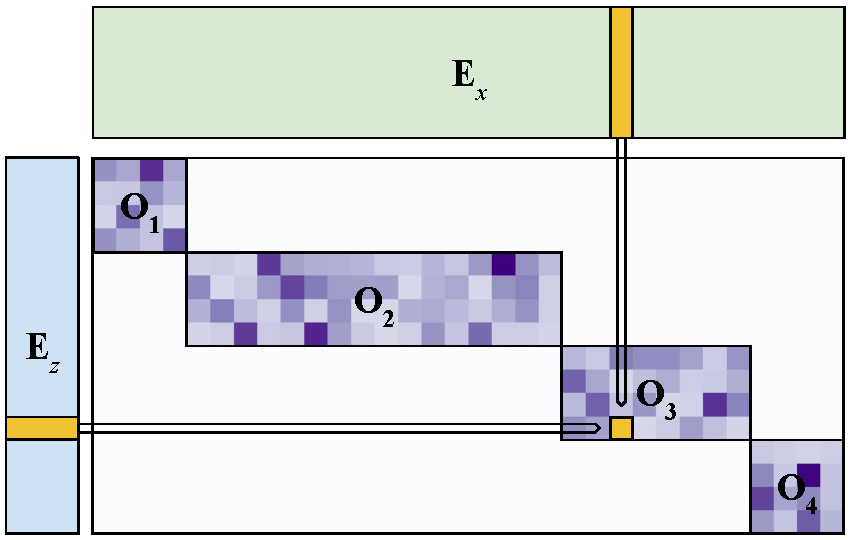
\includegraphics[height=1.7in]{img/blocksparse_mat_no_block.pdf}
\end{center}
\end{frame}

\begin{frame}
\frametitle{Technique 3: State Dropout}
\begin{itemize}
\item State dropout encourages broad state usage
\item At each batch, sample dropout mask $\mathbf{b} \in \set{0,1}^{Z}$
\end{itemize}
\begin{center}
\resizebox{0.75\width}{0.75\height}{
\normalsize%
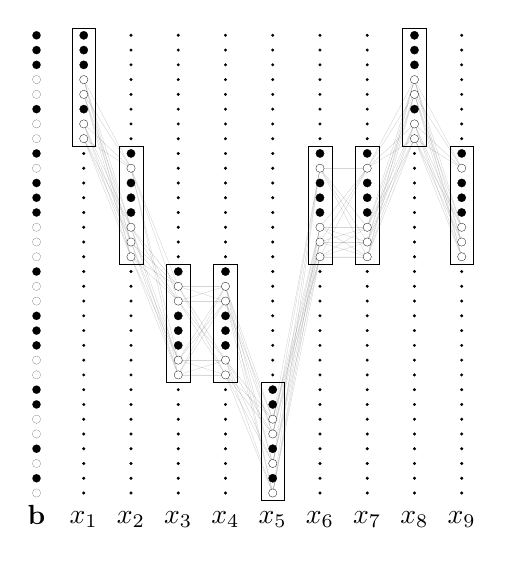
\begin{tikzpicture}%
\path[draw,line width=0.01pt,fill=white,radius=1.5pt] (0.0,0.0) circle;%
\path[draw,line width=0.01pt,fill=black,radius=1.5pt] (0.0,0.1875) circle;%
\path[draw,line width=0.01pt,fill=white,radius=1.5pt] (0.0,0.375) circle;%
\path[draw,line width=0.01pt,fill=black,radius=1.5pt] (0.0,0.5625) circle;%
\path[draw,line width=0.01pt,fill=white,radius=1.5pt] (0.0,0.75) circle;%
\path[draw,line width=0.01pt,fill=white,radius=1.5pt] (0.0,0.9375) circle;%
\path[draw,line width=0.01pt,fill=black,radius=1.5pt] (0.0,1.125) circle;%
\path[draw,line width=0.01pt,fill=black,radius=1.5pt] (0.0,1.3125) circle;%
\path[draw,line width=0.01pt,fill=white,radius=1.5pt] (0.0,1.5) circle;%
\path[draw,line width=0.01pt,fill=white,radius=1.5pt] (0.0,1.6875) circle;%
\path[draw,line width=0.01pt,fill=black,radius=1.5pt] (0.0,1.875) circle;%
\path[draw,line width=0.01pt,fill=black,radius=1.5pt] (0.0,2.0625) circle;%
\path[draw,line width=0.01pt,fill=black,radius=1.5pt] (0.0,2.25) circle;%
\path[draw,line width=0.01pt,fill=white,radius=1.5pt] (0.0,2.4375) circle;%
\path[draw,line width=0.01pt,fill=white,radius=1.5pt] (0.0,2.625) circle;%
\path[draw,line width=0.01pt,fill=black,radius=1.5pt] (0.0,2.8125) circle;%
\path[draw,line width=0.01pt,fill=white,radius=1.5pt] (0.0,3.0) circle;%
\path[draw,line width=0.01pt,fill=white,radius=1.5pt] (0.0,3.1875) circle;%
\path[draw,line width=0.01pt,fill=white,radius=1.5pt] (0.0,3.375) circle;%
\path[draw,line width=0.01pt,fill=black,radius=1.5pt] (0.0,3.5625) circle;%
\path[draw,line width=0.01pt,fill=black,radius=1.5pt] (0.0,3.75) circle;%
\path[draw,line width=0.01pt,fill=black,radius=1.5pt] (0.0,3.9375) circle;%
\path[draw,line width=0.01pt,fill=white,radius=1.5pt] (0.0,4.125) circle;%
\path[draw,line width=0.01pt,fill=black,radius=1.5pt] (0.0,4.3125) circle;%
\path[draw,line width=0.01pt,fill=white,radius=1.5pt] (0.0,4.5) circle;%
\path[draw,line width=0.01pt,fill=white,radius=1.5pt] (0.0,4.6875) circle;%
\path[draw,line width=0.01pt,fill=black,radius=1.5pt] (0.0,4.875) circle;%
\path[draw,line width=0.01pt,fill=white,radius=1.5pt] (0.0,5.0625) circle;%
\path[draw,line width=0.01pt,fill=white,radius=1.5pt] (0.0,5.25) circle;%
\path[draw,line width=0.01pt,fill=black,radius=1.5pt] (0.0,5.4375) circle;%
\path[draw,line width=0.01pt,fill=black,radius=1.5pt] (0.0,5.625) circle;%
\path[draw,line width=0.01pt,fill=black,radius=1.5pt] (0.0,5.8125) circle;%
\path[draw,line width=0.1pt,opacity=0.15,fill=black] (0.6,4.5) -- (1.2,3.0);%
\path[draw,line width=0.1pt,opacity=0.15,fill=black] (0.6,4.5) -- (1.2,3.1875);%
\path[draw,line width=0.1pt,opacity=0.15,fill=black] (0.6,4.5) -- (1.2,3.375);%
\path[draw,line width=0.1pt,opacity=0.15,fill=black] (0.6,4.5) -- (1.2,4.125);%
\path[draw,line width=0.1pt,opacity=0.15,fill=black] (0.6,4.6875) -- (1.2,3.0);%
\path[draw,line width=0.1pt,opacity=0.15,fill=black] (0.6,4.6875) -- (1.2,3.1875);%
\path[draw,line width=0.1pt,opacity=0.15,fill=black] (0.6,4.6875) -- (1.2,3.375);%
\path[draw,line width=0.1pt,opacity=0.15,fill=black] (0.6,4.6875) -- (1.2,4.125);%
\path[draw,line width=0.1pt,opacity=0.15,fill=black] (0.6,5.0625) -- (1.2,3.0);%
\path[draw,line width=0.1pt,opacity=0.15,fill=black] (0.6,5.0625) -- (1.2,3.1875);%
\path[draw,line width=0.1pt,opacity=0.15,fill=black] (0.6,5.0625) -- (1.2,3.375);%
\path[draw,line width=0.1pt,opacity=0.15,fill=black] (0.6,5.0625) -- (1.2,4.125);%
\path[draw,line width=0.1pt,opacity=0.15,fill=black] (0.6,5.25) -- (1.2,3.0);%
\path[draw,line width=0.1pt,opacity=0.15,fill=black] (0.6,5.25) -- (1.2,3.1875);%
\path[draw,line width=0.1pt,opacity=0.15,fill=black] (0.6,5.25) -- (1.2,3.375);%
\path[draw,line width=0.1pt,opacity=0.15,fill=black] (0.6,5.25) -- (1.2,4.125);%
\path[draw,line width=0.1pt,opacity=0.15,fill=black] (1.2,3.0) -- (1.8,1.5);%
\path[draw,line width=0.1pt,opacity=0.15,fill=black] (1.2,3.0) -- (1.8,1.6875);%
\path[draw,line width=0.1pt,opacity=0.15,fill=black] (1.2,3.0) -- (1.8,2.4375);%
\path[draw,line width=0.1pt,opacity=0.15,fill=black] (1.2,3.0) -- (1.8,2.625);%
\path[draw,line width=0.1pt,opacity=0.15,fill=black] (1.2,3.1875) -- (1.8,1.5);%
\path[draw,line width=0.1pt,opacity=0.15,fill=black] (1.2,3.1875) -- (1.8,1.6875);%
\path[draw,line width=0.1pt,opacity=0.15,fill=black] (1.2,3.1875) -- (1.8,2.4375);%
\path[draw,line width=0.1pt,opacity=0.15,fill=black] (1.2,3.1875) -- (1.8,2.625);%
\path[draw,line width=0.1pt,opacity=0.15,fill=black] (1.2,3.375) -- (1.8,1.5);%
\path[draw,line width=0.1pt,opacity=0.15,fill=black] (1.2,3.375) -- (1.8,1.6875);%
\path[draw,line width=0.1pt,opacity=0.15,fill=black] (1.2,3.375) -- (1.8,2.4375);%
\path[draw,line width=0.1pt,opacity=0.15,fill=black] (1.2,3.375) -- (1.8,2.625);%
\path[draw,line width=0.1pt,opacity=0.15,fill=black] (1.2,4.125) -- (1.8,1.5);%
\path[draw,line width=0.1pt,opacity=0.15,fill=black] (1.2,4.125) -- (1.8,1.6875);%
\path[draw,line width=0.1pt,opacity=0.15,fill=black] (1.2,4.125) -- (1.8,2.4375);%
\path[draw,line width=0.1pt,opacity=0.15,fill=black] (1.2,4.125) -- (1.8,2.625);%
\path[draw,line width=0.1pt,opacity=0.15,fill=black] (1.8,1.5) -- (2.4,1.5);%
\path[draw,line width=0.1pt,opacity=0.15,fill=black] (1.8,1.5) -- (2.4,1.6875);%
\path[draw,line width=0.1pt,opacity=0.15,fill=black] (1.8,1.5) -- (2.4,2.4375);%
\path[draw,line width=0.1pt,opacity=0.15,fill=black] (1.8,1.5) -- (2.4,2.625);%
\path[draw,line width=0.1pt,opacity=0.15,fill=black] (1.8,1.6875) -- (2.4,1.5);%
\path[draw,line width=0.1pt,opacity=0.15,fill=black] (1.8,1.6875) -- (2.4,1.6875);%
\path[draw,line width=0.1pt,opacity=0.15,fill=black] (1.8,1.6875) -- (2.4,2.4375);%
\path[draw,line width=0.1pt,opacity=0.15,fill=black] (1.8,1.6875) -- (2.4,2.625);%
\path[draw,line width=0.1pt,opacity=0.15,fill=black] (1.8,2.4375) -- (2.4,1.5);%
\path[draw,line width=0.1pt,opacity=0.15,fill=black] (1.8,2.4375) -- (2.4,1.6875);%
\path[draw,line width=0.1pt,opacity=0.15,fill=black] (1.8,2.4375) -- (2.4,2.4375);%
\path[draw,line width=0.1pt,opacity=0.15,fill=black] (1.8,2.4375) -- (2.4,2.625);%
\path[draw,line width=0.1pt,opacity=0.15,fill=black] (1.8,2.625) -- (2.4,1.5);%
\path[draw,line width=0.1pt,opacity=0.15,fill=black] (1.8,2.625) -- (2.4,1.6875);%
\path[draw,line width=0.1pt,opacity=0.15,fill=black] (1.8,2.625) -- (2.4,2.4375);%
\path[draw,line width=0.1pt,opacity=0.15,fill=black] (1.8,2.625) -- (2.4,2.625);%
\path[draw,line width=0.1pt,opacity=0.15,fill=black] (2.4,1.5) -- (3.0,0.0);%
\path[draw,line width=0.1pt,opacity=0.15,fill=black] (2.4,1.5) -- (3.0,0.375);%
\path[draw,line width=0.1pt,opacity=0.15,fill=black] (2.4,1.5) -- (3.0,0.75);%
\path[draw,line width=0.1pt,opacity=0.15,fill=black] (2.4,1.5) -- (3.0,0.9375);%
\path[draw,line width=0.1pt,opacity=0.15,fill=black] (2.4,1.6875) -- (3.0,0.0);%
\path[draw,line width=0.1pt,opacity=0.15,fill=black] (2.4,1.6875) -- (3.0,0.375);%
\path[draw,line width=0.1pt,opacity=0.15,fill=black] (2.4,1.6875) -- (3.0,0.75);%
\path[draw,line width=0.1pt,opacity=0.15,fill=black] (2.4,1.6875) -- (3.0,0.9375);%
\path[draw,line width=0.1pt,opacity=0.15,fill=black] (2.4,2.4375) -- (3.0,0.0);%
\path[draw,line width=0.1pt,opacity=0.15,fill=black] (2.4,2.4375) -- (3.0,0.375);%
\path[draw,line width=0.1pt,opacity=0.15,fill=black] (2.4,2.4375) -- (3.0,0.75);%
\path[draw,line width=0.1pt,opacity=0.15,fill=black] (2.4,2.4375) -- (3.0,0.9375);%
\path[draw,line width=0.1pt,opacity=0.15,fill=black] (2.4,2.625) -- (3.0,0.0);%
\path[draw,line width=0.1pt,opacity=0.15,fill=black] (2.4,2.625) -- (3.0,0.375);%
\path[draw,line width=0.1pt,opacity=0.15,fill=black] (2.4,2.625) -- (3.0,0.75);%
\path[draw,line width=0.1pt,opacity=0.15,fill=black] (2.4,2.625) -- (3.0,0.9375);%
\path[draw,line width=0.1pt,opacity=0.15,fill=black] (3.0,0.0) -- (3.6,3.0);%
\path[draw,line width=0.1pt,opacity=0.15,fill=black] (3.0,0.0) -- (3.6,3.1875);%
\path[draw,line width=0.1pt,opacity=0.15,fill=black] (3.0,0.0) -- (3.6,3.375);%
\path[draw,line width=0.1pt,opacity=0.15,fill=black] (3.0,0.0) -- (3.6,4.125);%
\path[draw,line width=0.1pt,opacity=0.15,fill=black] (3.0,0.375) -- (3.6,3.0);%
\path[draw,line width=0.1pt,opacity=0.15,fill=black] (3.0,0.375) -- (3.6,3.1875);%
\path[draw,line width=0.1pt,opacity=0.15,fill=black] (3.0,0.375) -- (3.6,3.375);%
\path[draw,line width=0.1pt,opacity=0.15,fill=black] (3.0,0.375) -- (3.6,4.125);%
\path[draw,line width=0.1pt,opacity=0.15,fill=black] (3.0,0.75) -- (3.6,3.0);%
\path[draw,line width=0.1pt,opacity=0.15,fill=black] (3.0,0.75) -- (3.6,3.1875);%
\path[draw,line width=0.1pt,opacity=0.15,fill=black] (3.0,0.75) -- (3.6,3.375);%
\path[draw,line width=0.1pt,opacity=0.15,fill=black] (3.0,0.75) -- (3.6,4.125);%
\path[draw,line width=0.1pt,opacity=0.15,fill=black] (3.0,0.9375) -- (3.6,3.0);%
\path[draw,line width=0.1pt,opacity=0.15,fill=black] (3.0,0.9375) -- (3.6,3.1875);%
\path[draw,line width=0.1pt,opacity=0.15,fill=black] (3.0,0.9375) -- (3.6,3.375);%
\path[draw,line width=0.1pt,opacity=0.15,fill=black] (3.0,0.9375) -- (3.6,4.125);%
\path[draw,line width=0.1pt,opacity=0.15,fill=black] (3.6,3.0) -- (4.2,3.0);%
\path[draw,line width=0.1pt,opacity=0.15,fill=black] (3.6,3.0) -- (4.2,3.1875);%
\path[draw,line width=0.1pt,opacity=0.15,fill=black] (3.6,3.0) -- (4.2,3.375);%
\path[draw,line width=0.1pt,opacity=0.15,fill=black] (3.6,3.0) -- (4.2,4.125);%
\path[draw,line width=0.1pt,opacity=0.15,fill=black] (3.6,3.1875) -- (4.2,3.0);%
\path[draw,line width=0.1pt,opacity=0.15,fill=black] (3.6,3.1875) -- (4.2,3.1875);%
\path[draw,line width=0.1pt,opacity=0.15,fill=black] (3.6,3.1875) -- (4.2,3.375);%
\path[draw,line width=0.1pt,opacity=0.15,fill=black] (3.6,3.1875) -- (4.2,4.125);%
\path[draw,line width=0.1pt,opacity=0.15,fill=black] (3.6,3.375) -- (4.2,3.0);%
\path[draw,line width=0.1pt,opacity=0.15,fill=black] (3.6,3.375) -- (4.2,3.1875);%
\path[draw,line width=0.1pt,opacity=0.15,fill=black] (3.6,3.375) -- (4.2,3.375);%
\path[draw,line width=0.1pt,opacity=0.15,fill=black] (3.6,3.375) -- (4.2,4.125);%
\path[draw,line width=0.1pt,opacity=0.15,fill=black] (3.6,4.125) -- (4.2,3.0);%
\path[draw,line width=0.1pt,opacity=0.15,fill=black] (3.6,4.125) -- (4.2,3.1875);%
\path[draw,line width=0.1pt,opacity=0.15,fill=black] (3.6,4.125) -- (4.2,3.375);%
\path[draw,line width=0.1pt,opacity=0.15,fill=black] (3.6,4.125) -- (4.2,4.125);%
\path[draw,line width=0.1pt,opacity=0.15,fill=black] (4.2,3.0) -- (4.8,4.5);%
\path[draw,line width=0.1pt,opacity=0.15,fill=black] (4.2,3.0) -- (4.8,4.6875);%
\path[draw,line width=0.1pt,opacity=0.15,fill=black] (4.2,3.0) -- (4.8,5.0625);%
\path[draw,line width=0.1pt,opacity=0.15,fill=black] (4.2,3.0) -- (4.8,5.25);%
\path[draw,line width=0.1pt,opacity=0.15,fill=black] (4.2,3.1875) -- (4.8,4.5);%
\path[draw,line width=0.1pt,opacity=0.15,fill=black] (4.2,3.1875) -- (4.8,4.6875);%
\path[draw,line width=0.1pt,opacity=0.15,fill=black] (4.2,3.1875) -- (4.8,5.0625);%
\path[draw,line width=0.1pt,opacity=0.15,fill=black] (4.2,3.1875) -- (4.8,5.25);%
\path[draw,line width=0.1pt,opacity=0.15,fill=black] (4.2,3.375) -- (4.8,4.5);%
\path[draw,line width=0.1pt,opacity=0.15,fill=black] (4.2,3.375) -- (4.8,4.6875);%
\path[draw,line width=0.1pt,opacity=0.15,fill=black] (4.2,3.375) -- (4.8,5.0625);%
\path[draw,line width=0.1pt,opacity=0.15,fill=black] (4.2,3.375) -- (4.8,5.25);%
\path[draw,line width=0.1pt,opacity=0.15,fill=black] (4.2,4.125) -- (4.8,4.5);%
\path[draw,line width=0.1pt,opacity=0.15,fill=black] (4.2,4.125) -- (4.8,4.6875);%
\path[draw,line width=0.1pt,opacity=0.15,fill=black] (4.2,4.125) -- (4.8,5.0625);%
\path[draw,line width=0.1pt,opacity=0.15,fill=black] (4.2,4.125) -- (4.8,5.25);%
\path[draw,line width=0.1pt,opacity=0.15,fill=black] (4.8,4.5) -- (5.4,3.0);%
\path[draw,line width=0.1pt,opacity=0.15,fill=black] (4.8,4.5) -- (5.4,3.1875);%
\path[draw,line width=0.1pt,opacity=0.15,fill=black] (4.8,4.5) -- (5.4,3.375);%
\path[draw,line width=0.1pt,opacity=0.15,fill=black] (4.8,4.5) -- (5.4,4.125);%
\path[draw,line width=0.1pt,opacity=0.15,fill=black] (4.8,4.6875) -- (5.4,3.0);%
\path[draw,line width=0.1pt,opacity=0.15,fill=black] (4.8,4.6875) -- (5.4,3.1875);%
\path[draw,line width=0.1pt,opacity=0.15,fill=black] (4.8,4.6875) -- (5.4,3.375);%
\path[draw,line width=0.1pt,opacity=0.15,fill=black] (4.8,4.6875) -- (5.4,4.125);%
\path[draw,line width=0.1pt,opacity=0.15,fill=black] (4.8,5.0625) -- (5.4,3.0);%
\path[draw,line width=0.1pt,opacity=0.15,fill=black] (4.8,5.0625) -- (5.4,3.1875);%
\path[draw,line width=0.1pt,opacity=0.15,fill=black] (4.8,5.0625) -- (5.4,3.375);%
\path[draw,line width=0.1pt,opacity=0.15,fill=black] (4.8,5.0625) -- (5.4,4.125);%
\path[draw,line width=0.1pt,opacity=0.15,fill=black] (4.8,5.25) -- (5.4,3.0);%
\path[draw,line width=0.1pt,opacity=0.15,fill=black] (4.8,5.25) -- (5.4,3.1875);%
\path[draw,line width=0.1pt,opacity=0.15,fill=black] (4.8,5.25) -- (5.4,3.375);%
\path[draw,line width=0.1pt,opacity=0.15,fill=black] (4.8,5.25) -- (5.4,4.125);%
\path[draw,line width=0.2pt] (0.45,4.40625) rectangle (0.75,5.90625);%
\path[draw,line width=0.2pt] (1.05,2.90625) rectangle (1.35,4.40625);%
\path[draw,line width=0.2pt] (1.65,1.40625) rectangle (1.95,2.90625);%
\path[draw,line width=0.2pt] (2.25,1.40625) rectangle (2.55,2.90625);%
\path[draw,line width=0.2pt] (2.85,-0.09375) rectangle (3.15,1.40625);%
\path[draw,line width=0.2pt] (3.45,2.90625) rectangle (3.75,4.40625);%
\path[draw,line width=0.2pt] (4.05,2.90625) rectangle (4.35,4.40625);%
\path[draw,line width=0.2pt] (4.65,4.40625) rectangle (4.95,5.90625);%
\path[draw,line width=0.2pt] (5.25,2.90625) rectangle (5.55,4.40625);%
\node[inner sep=0] (b) at (0.0,-0.28125) {$\mathbf{b}$};%
\node (x1) at (0.6,-0.3375) {$x_1$};%
\node (x2) at (1.2,-0.3375) {$x_2$};%
\node (x3) at (1.8,-0.3375) {$x_3$};%
\node (x4) at (2.4,-0.3375) {$x_4$};%
\node (x5) at (3.0,-0.3375) {$x_5$};%
\node (x6) at (3.6,-0.3375) {$x_6$};%
\node (x7) at (4.2,-0.3375) {$x_7$};%
\node (x8) at (4.8,-0.3375) {$x_8$};%
\node (x9) at (5.4,-0.3375) {$x_9$};%
\path[draw,line width=0.1pt,fill=black,radius=0.5pt] (0.6,0.0) circle;%
\path[draw,line width=0.1pt,fill=black,radius=0.5pt] (0.6,0.1875) circle;%
\path[draw,line width=0.1pt,fill=black,radius=0.5pt] (0.6,0.375) circle;%
\path[draw,line width=0.1pt,fill=black,radius=0.5pt] (0.6,0.5625) circle;%
\path[draw,line width=0.1pt,fill=black,radius=0.5pt] (0.6,0.75) circle;%
\path[draw,line width=0.1pt,fill=black,radius=0.5pt] (0.6,0.9375) circle;%
\path[draw,line width=0.1pt,fill=black,radius=0.5pt] (0.6,1.125) circle;%
\path[draw,line width=0.1pt,fill=black,radius=0.5pt] (0.6,1.3125) circle;%
\path[draw,line width=0.1pt,fill=black,radius=0.5pt] (0.6,1.5) circle;%
\path[draw,line width=0.1pt,fill=black,radius=0.5pt] (0.6,1.6875) circle;%
\path[draw,line width=0.1pt,fill=black,radius=0.5pt] (0.6,1.875) circle;%
\path[draw,line width=0.1pt,fill=black,radius=0.5pt] (0.6,2.0625) circle;%
\path[draw,line width=0.1pt,fill=black,radius=0.5pt] (0.6,2.25) circle;%
\path[draw,line width=0.1pt,fill=black,radius=0.5pt] (0.6,2.4375) circle;%
\path[draw,line width=0.1pt,fill=black,radius=0.5pt] (0.6,2.625) circle;%
\path[draw,line width=0.1pt,fill=black,radius=0.5pt] (0.6,2.8125) circle;%
\path[draw,line width=0.1pt,fill=black,radius=0.5pt] (0.6,3.0) circle;%
\path[draw,line width=0.1pt,fill=black,radius=0.5pt] (0.6,3.1875) circle;%
\path[draw,line width=0.1pt,fill=black,radius=0.5pt] (0.6,3.375) circle;%
\path[draw,line width=0.1pt,fill=black,radius=0.5pt] (0.6,3.5625) circle;%
\path[draw,line width=0.1pt,fill=black,radius=0.5pt] (0.6,3.75) circle;%
\path[draw,line width=0.1pt,fill=black,radius=0.5pt] (0.6,3.9375) circle;%
\path[draw,line width=0.1pt,fill=black,radius=0.5pt] (0.6,4.125) circle;%
\path[draw,line width=0.1pt,fill=black,radius=0.5pt] (0.6,4.3125) circle;%
\path[draw,line width=0.1pt,fill=white,radius=1.5pt] (0.6,4.5) circle;%
\path[draw,line width=0.1pt,fill=white,radius=1.5pt] (0.6,4.6875) circle;%
\path[draw,line width=0.1pt,fill=black,radius=1.5pt] (0.6,4.875) circle;%
\path[draw,line width=0.1pt,fill=white,radius=1.5pt] (0.6,5.0625) circle;%
\path[draw,line width=0.1pt,fill=white,radius=1.5pt] (0.6,5.25) circle;%
\path[draw,line width=0.1pt,fill=black,radius=1.5pt] (0.6,5.4375) circle;%
\path[draw,line width=0.1pt,fill=black,radius=1.5pt] (0.6,5.625) circle;%
\path[draw,line width=0.1pt,fill=black,radius=1.5pt] (0.6,5.8125) circle;%
\path[draw,line width=0.1pt,fill=black,radius=0.5pt] (1.2,0.0) circle;%
\path[draw,line width=0.1pt,fill=black,radius=0.5pt] (1.2,0.1875) circle;%
\path[draw,line width=0.1pt,fill=black,radius=0.5pt] (1.2,0.375) circle;%
\path[draw,line width=0.1pt,fill=black,radius=0.5pt] (1.2,0.5625) circle;%
\path[draw,line width=0.1pt,fill=black,radius=0.5pt] (1.2,0.75) circle;%
\path[draw,line width=0.1pt,fill=black,radius=0.5pt] (1.2,0.9375) circle;%
\path[draw,line width=0.1pt,fill=black,radius=0.5pt] (1.2,1.125) circle;%
\path[draw,line width=0.1pt,fill=black,radius=0.5pt] (1.2,1.3125) circle;%
\path[draw,line width=0.1pt,fill=black,radius=0.5pt] (1.2,1.5) circle;%
\path[draw,line width=0.1pt,fill=black,radius=0.5pt] (1.2,1.6875) circle;%
\path[draw,line width=0.1pt,fill=black,radius=0.5pt] (1.2,1.875) circle;%
\path[draw,line width=0.1pt,fill=black,radius=0.5pt] (1.2,2.0625) circle;%
\path[draw,line width=0.1pt,fill=black,radius=0.5pt] (1.2,2.25) circle;%
\path[draw,line width=0.1pt,fill=black,radius=0.5pt] (1.2,2.4375) circle;%
\path[draw,line width=0.1pt,fill=black,radius=0.5pt] (1.2,2.625) circle;%
\path[draw,line width=0.1pt,fill=black,radius=0.5pt] (1.2,2.8125) circle;%
\path[draw,line width=0.1pt,fill=white,radius=1.5pt] (1.2,3.0) circle;%
\path[draw,line width=0.1pt,fill=white,radius=1.5pt] (1.2,3.1875) circle;%
\path[draw,line width=0.1pt,fill=white,radius=1.5pt] (1.2,3.375) circle;%
\path[draw,line width=0.1pt,fill=black,radius=1.5pt] (1.2,3.5625) circle;%
\path[draw,line width=0.1pt,fill=black,radius=1.5pt] (1.2,3.75) circle;%
\path[draw,line width=0.1pt,fill=black,radius=1.5pt] (1.2,3.9375) circle;%
\path[draw,line width=0.1pt,fill=white,radius=1.5pt] (1.2,4.125) circle;%
\path[draw,line width=0.1pt,fill=black,radius=1.5pt] (1.2,4.3125) circle;%
\path[draw,line width=0.1pt,fill=black,radius=0.5pt] (1.2,4.5) circle;%
\path[draw,line width=0.1pt,fill=black,radius=0.5pt] (1.2,4.6875) circle;%
\path[draw,line width=0.1pt,fill=black,radius=0.5pt] (1.2,4.875) circle;%
\path[draw,line width=0.1pt,fill=black,radius=0.5pt] (1.2,5.0625) circle;%
\path[draw,line width=0.1pt,fill=black,radius=0.5pt] (1.2,5.25) circle;%
\path[draw,line width=0.1pt,fill=black,radius=0.5pt] (1.2,5.4375) circle;%
\path[draw,line width=0.1pt,fill=black,radius=0.5pt] (1.2,5.625) circle;%
\path[draw,line width=0.1pt,fill=black,radius=0.5pt] (1.2,5.8125) circle;%
\path[draw,line width=0.1pt,fill=black,radius=0.5pt] (1.8,0.0) circle;%
\path[draw,line width=0.1pt,fill=black,radius=0.5pt] (1.8,0.1875) circle;%
\path[draw,line width=0.1pt,fill=black,radius=0.5pt] (1.8,0.375) circle;%
\path[draw,line width=0.1pt,fill=black,radius=0.5pt] (1.8,0.5625) circle;%
\path[draw,line width=0.1pt,fill=black,radius=0.5pt] (1.8,0.75) circle;%
\path[draw,line width=0.1pt,fill=black,radius=0.5pt] (1.8,0.9375) circle;%
\path[draw,line width=0.1pt,fill=black,radius=0.5pt] (1.8,1.125) circle;%
\path[draw,line width=0.1pt,fill=black,radius=0.5pt] (1.8,1.3125) circle;%
\path[draw,line width=0.1pt,fill=white,radius=1.5pt] (1.8,1.5) circle;%
\path[draw,line width=0.1pt,fill=white,radius=1.5pt] (1.8,1.6875) circle;%
\path[draw,line width=0.1pt,fill=black,radius=1.5pt] (1.8,1.875) circle;%
\path[draw,line width=0.1pt,fill=black,radius=1.5pt] (1.8,2.0625) circle;%
\path[draw,line width=0.1pt,fill=black,radius=1.5pt] (1.8,2.25) circle;%
\path[draw,line width=0.1pt,fill=white,radius=1.5pt] (1.8,2.4375) circle;%
\path[draw,line width=0.1pt,fill=white,radius=1.5pt] (1.8,2.625) circle;%
\path[draw,line width=0.1pt,fill=black,radius=1.5pt] (1.8,2.8125) circle;%
\path[draw,line width=0.1pt,fill=black,radius=0.5pt] (1.8,3.0) circle;%
\path[draw,line width=0.1pt,fill=black,radius=0.5pt] (1.8,3.1875) circle;%
\path[draw,line width=0.1pt,fill=black,radius=0.5pt] (1.8,3.375) circle;%
\path[draw,line width=0.1pt,fill=black,radius=0.5pt] (1.8,3.5625) circle;%
\path[draw,line width=0.1pt,fill=black,radius=0.5pt] (1.8,3.75) circle;%
\path[draw,line width=0.1pt,fill=black,radius=0.5pt] (1.8,3.9375) circle;%
\path[draw,line width=0.1pt,fill=black,radius=0.5pt] (1.8,4.125) circle;%
\path[draw,line width=0.1pt,fill=black,radius=0.5pt] (1.8,4.3125) circle;%
\path[draw,line width=0.1pt,fill=black,radius=0.5pt] (1.8,4.5) circle;%
\path[draw,line width=0.1pt,fill=black,radius=0.5pt] (1.8,4.6875) circle;%
\path[draw,line width=0.1pt,fill=black,radius=0.5pt] (1.8,4.875) circle;%
\path[draw,line width=0.1pt,fill=black,radius=0.5pt] (1.8,5.0625) circle;%
\path[draw,line width=0.1pt,fill=black,radius=0.5pt] (1.8,5.25) circle;%
\path[draw,line width=0.1pt,fill=black,radius=0.5pt] (1.8,5.4375) circle;%
\path[draw,line width=0.1pt,fill=black,radius=0.5pt] (1.8,5.625) circle;%
\path[draw,line width=0.1pt,fill=black,radius=0.5pt] (1.8,5.8125) circle;%
\path[draw,line width=0.1pt,fill=black,radius=0.5pt] (2.4,0.0) circle;%
\path[draw,line width=0.1pt,fill=black,radius=0.5pt] (2.4,0.1875) circle;%
\path[draw,line width=0.1pt,fill=black,radius=0.5pt] (2.4,0.375) circle;%
\path[draw,line width=0.1pt,fill=black,radius=0.5pt] (2.4,0.5625) circle;%
\path[draw,line width=0.1pt,fill=black,radius=0.5pt] (2.4,0.75) circle;%
\path[draw,line width=0.1pt,fill=black,radius=0.5pt] (2.4,0.9375) circle;%
\path[draw,line width=0.1pt,fill=black,radius=0.5pt] (2.4,1.125) circle;%
\path[draw,line width=0.1pt,fill=black,radius=0.5pt] (2.4,1.3125) circle;%
\path[draw,line width=0.1pt,fill=white,radius=1.5pt] (2.4,1.5) circle;%
\path[draw,line width=0.1pt,fill=white,radius=1.5pt] (2.4,1.6875) circle;%
\path[draw,line width=0.1pt,fill=black,radius=1.5pt] (2.4,1.875) circle;%
\path[draw,line width=0.1pt,fill=black,radius=1.5pt] (2.4,2.0625) circle;%
\path[draw,line width=0.1pt,fill=black,radius=1.5pt] (2.4,2.25) circle;%
\path[draw,line width=0.1pt,fill=white,radius=1.5pt] (2.4,2.4375) circle;%
\path[draw,line width=0.1pt,fill=white,radius=1.5pt] (2.4,2.625) circle;%
\path[draw,line width=0.1pt,fill=black,radius=1.5pt] (2.4,2.8125) circle;%
\path[draw,line width=0.1pt,fill=black,radius=0.5pt] (2.4,3.0) circle;%
\path[draw,line width=0.1pt,fill=black,radius=0.5pt] (2.4,3.1875) circle;%
\path[draw,line width=0.1pt,fill=black,radius=0.5pt] (2.4,3.375) circle;%
\path[draw,line width=0.1pt,fill=black,radius=0.5pt] (2.4,3.5625) circle;%
\path[draw,line width=0.1pt,fill=black,radius=0.5pt] (2.4,3.75) circle;%
\path[draw,line width=0.1pt,fill=black,radius=0.5pt] (2.4,3.9375) circle;%
\path[draw,line width=0.1pt,fill=black,radius=0.5pt] (2.4,4.125) circle;%
\path[draw,line width=0.1pt,fill=black,radius=0.5pt] (2.4,4.3125) circle;%
\path[draw,line width=0.1pt,fill=black,radius=0.5pt] (2.4,4.5) circle;%
\path[draw,line width=0.1pt,fill=black,radius=0.5pt] (2.4,4.6875) circle;%
\path[draw,line width=0.1pt,fill=black,radius=0.5pt] (2.4,4.875) circle;%
\path[draw,line width=0.1pt,fill=black,radius=0.5pt] (2.4,5.0625) circle;%
\path[draw,line width=0.1pt,fill=black,radius=0.5pt] (2.4,5.25) circle;%
\path[draw,line width=0.1pt,fill=black,radius=0.5pt] (2.4,5.4375) circle;%
\path[draw,line width=0.1pt,fill=black,radius=0.5pt] (2.4,5.625) circle;%
\path[draw,line width=0.1pt,fill=black,radius=0.5pt] (2.4,5.8125) circle;%
\path[draw,line width=0.1pt,fill=white,radius=1.5pt] (3.0,0.0) circle;%
\path[draw,line width=0.1pt,fill=black,radius=1.5pt] (3.0,0.1875) circle;%
\path[draw,line width=0.1pt,fill=white,radius=1.5pt] (3.0,0.375) circle;%
\path[draw,line width=0.1pt,fill=black,radius=1.5pt] (3.0,0.5625) circle;%
\path[draw,line width=0.1pt,fill=white,radius=1.5pt] (3.0,0.75) circle;%
\path[draw,line width=0.1pt,fill=white,radius=1.5pt] (3.0,0.9375) circle;%
\path[draw,line width=0.1pt,fill=black,radius=1.5pt] (3.0,1.125) circle;%
\path[draw,line width=0.1pt,fill=black,radius=1.5pt] (3.0,1.3125) circle;%
\path[draw,line width=0.1pt,fill=black,radius=0.5pt] (3.0,1.5) circle;%
\path[draw,line width=0.1pt,fill=black,radius=0.5pt] (3.0,1.6875) circle;%
\path[draw,line width=0.1pt,fill=black,radius=0.5pt] (3.0,1.875) circle;%
\path[draw,line width=0.1pt,fill=black,radius=0.5pt] (3.0,2.0625) circle;%
\path[draw,line width=0.1pt,fill=black,radius=0.5pt] (3.0,2.25) circle;%
\path[draw,line width=0.1pt,fill=black,radius=0.5pt] (3.0,2.4375) circle;%
\path[draw,line width=0.1pt,fill=black,radius=0.5pt] (3.0,2.625) circle;%
\path[draw,line width=0.1pt,fill=black,radius=0.5pt] (3.0,2.8125) circle;%
\path[draw,line width=0.1pt,fill=black,radius=0.5pt] (3.0,3.0) circle;%
\path[draw,line width=0.1pt,fill=black,radius=0.5pt] (3.0,3.1875) circle;%
\path[draw,line width=0.1pt,fill=black,radius=0.5pt] (3.0,3.375) circle;%
\path[draw,line width=0.1pt,fill=black,radius=0.5pt] (3.0,3.5625) circle;%
\path[draw,line width=0.1pt,fill=black,radius=0.5pt] (3.0,3.75) circle;%
\path[draw,line width=0.1pt,fill=black,radius=0.5pt] (3.0,3.9375) circle;%
\path[draw,line width=0.1pt,fill=black,radius=0.5pt] (3.0,4.125) circle;%
\path[draw,line width=0.1pt,fill=black,radius=0.5pt] (3.0,4.3125) circle;%
\path[draw,line width=0.1pt,fill=black,radius=0.5pt] (3.0,4.5) circle;%
\path[draw,line width=0.1pt,fill=black,radius=0.5pt] (3.0,4.6875) circle;%
\path[draw,line width=0.1pt,fill=black,radius=0.5pt] (3.0,4.875) circle;%
\path[draw,line width=0.1pt,fill=black,radius=0.5pt] (3.0,5.0625) circle;%
\path[draw,line width=0.1pt,fill=black,radius=0.5pt] (3.0,5.25) circle;%
\path[draw,line width=0.1pt,fill=black,radius=0.5pt] (3.0,5.4375) circle;%
\path[draw,line width=0.1pt,fill=black,radius=0.5pt] (3.0,5.625) circle;%
\path[draw,line width=0.1pt,fill=black,radius=0.5pt] (3.0,5.8125) circle;%
\path[draw,line width=0.1pt,fill=black,radius=0.5pt] (3.6,0.0) circle;%
\path[draw,line width=0.1pt,fill=black,radius=0.5pt] (3.6,0.1875) circle;%
\path[draw,line width=0.1pt,fill=black,radius=0.5pt] (3.6,0.375) circle;%
\path[draw,line width=0.1pt,fill=black,radius=0.5pt] (3.6,0.5625) circle;%
\path[draw,line width=0.1pt,fill=black,radius=0.5pt] (3.6,0.75) circle;%
\path[draw,line width=0.1pt,fill=black,radius=0.5pt] (3.6,0.9375) circle;%
\path[draw,line width=0.1pt,fill=black,radius=0.5pt] (3.6,1.125) circle;%
\path[draw,line width=0.1pt,fill=black,radius=0.5pt] (3.6,1.3125) circle;%
\path[draw,line width=0.1pt,fill=black,radius=0.5pt] (3.6,1.5) circle;%
\path[draw,line width=0.1pt,fill=black,radius=0.5pt] (3.6,1.6875) circle;%
\path[draw,line width=0.1pt,fill=black,radius=0.5pt] (3.6,1.875) circle;%
\path[draw,line width=0.1pt,fill=black,radius=0.5pt] (3.6,2.0625) circle;%
\path[draw,line width=0.1pt,fill=black,radius=0.5pt] (3.6,2.25) circle;%
\path[draw,line width=0.1pt,fill=black,radius=0.5pt] (3.6,2.4375) circle;%
\path[draw,line width=0.1pt,fill=black,radius=0.5pt] (3.6,2.625) circle;%
\path[draw,line width=0.1pt,fill=black,radius=0.5pt] (3.6,2.8125) circle;%
\path[draw,line width=0.1pt,fill=white,radius=1.5pt] (3.6,3.0) circle;%
\path[draw,line width=0.1pt,fill=white,radius=1.5pt] (3.6,3.1875) circle;%
\path[draw,line width=0.1pt,fill=white,radius=1.5pt] (3.6,3.375) circle;%
\path[draw,line width=0.1pt,fill=black,radius=1.5pt] (3.6,3.5625) circle;%
\path[draw,line width=0.1pt,fill=black,radius=1.5pt] (3.6,3.75) circle;%
\path[draw,line width=0.1pt,fill=black,radius=1.5pt] (3.6,3.9375) circle;%
\path[draw,line width=0.1pt,fill=white,radius=1.5pt] (3.6,4.125) circle;%
\path[draw,line width=0.1pt,fill=black,radius=1.5pt] (3.6,4.3125) circle;%
\path[draw,line width=0.1pt,fill=black,radius=0.5pt] (3.6,4.5) circle;%
\path[draw,line width=0.1pt,fill=black,radius=0.5pt] (3.6,4.6875) circle;%
\path[draw,line width=0.1pt,fill=black,radius=0.5pt] (3.6,4.875) circle;%
\path[draw,line width=0.1pt,fill=black,radius=0.5pt] (3.6,5.0625) circle;%
\path[draw,line width=0.1pt,fill=black,radius=0.5pt] (3.6,5.25) circle;%
\path[draw,line width=0.1pt,fill=black,radius=0.5pt] (3.6,5.4375) circle;%
\path[draw,line width=0.1pt,fill=black,radius=0.5pt] (3.6,5.625) circle;%
\path[draw,line width=0.1pt,fill=black,radius=0.5pt] (3.6,5.8125) circle;%
\path[draw,line width=0.1pt,fill=black,radius=0.5pt] (4.2,0.0) circle;%
\path[draw,line width=0.1pt,fill=black,radius=0.5pt] (4.2,0.1875) circle;%
\path[draw,line width=0.1pt,fill=black,radius=0.5pt] (4.2,0.375) circle;%
\path[draw,line width=0.1pt,fill=black,radius=0.5pt] (4.2,0.5625) circle;%
\path[draw,line width=0.1pt,fill=black,radius=0.5pt] (4.2,0.75) circle;%
\path[draw,line width=0.1pt,fill=black,radius=0.5pt] (4.2,0.9375) circle;%
\path[draw,line width=0.1pt,fill=black,radius=0.5pt] (4.2,1.125) circle;%
\path[draw,line width=0.1pt,fill=black,radius=0.5pt] (4.2,1.3125) circle;%
\path[draw,line width=0.1pt,fill=black,radius=0.5pt] (4.2,1.5) circle;%
\path[draw,line width=0.1pt,fill=black,radius=0.5pt] (4.2,1.6875) circle;%
\path[draw,line width=0.1pt,fill=black,radius=0.5pt] (4.2,1.875) circle;%
\path[draw,line width=0.1pt,fill=black,radius=0.5pt] (4.2,2.0625) circle;%
\path[draw,line width=0.1pt,fill=black,radius=0.5pt] (4.2,2.25) circle;%
\path[draw,line width=0.1pt,fill=black,radius=0.5pt] (4.2,2.4375) circle;%
\path[draw,line width=0.1pt,fill=black,radius=0.5pt] (4.2,2.625) circle;%
\path[draw,line width=0.1pt,fill=black,radius=0.5pt] (4.2,2.8125) circle;%
\path[draw,line width=0.1pt,fill=white,radius=1.5pt] (4.2,3.0) circle;%
\path[draw,line width=0.1pt,fill=white,radius=1.5pt] (4.2,3.1875) circle;%
\path[draw,line width=0.1pt,fill=white,radius=1.5pt] (4.2,3.375) circle;%
\path[draw,line width=0.1pt,fill=black,radius=1.5pt] (4.2,3.5625) circle;%
\path[draw,line width=0.1pt,fill=black,radius=1.5pt] (4.2,3.75) circle;%
\path[draw,line width=0.1pt,fill=black,radius=1.5pt] (4.2,3.9375) circle;%
\path[draw,line width=0.1pt,fill=white,radius=1.5pt] (4.2,4.125) circle;%
\path[draw,line width=0.1pt,fill=black,radius=1.5pt] (4.2,4.3125) circle;%
\path[draw,line width=0.1pt,fill=black,radius=0.5pt] (4.2,4.5) circle;%
\path[draw,line width=0.1pt,fill=black,radius=0.5pt] (4.2,4.6875) circle;%
\path[draw,line width=0.1pt,fill=black,radius=0.5pt] (4.2,4.875) circle;%
\path[draw,line width=0.1pt,fill=black,radius=0.5pt] (4.2,5.0625) circle;%
\path[draw,line width=0.1pt,fill=black,radius=0.5pt] (4.2,5.25) circle;%
\path[draw,line width=0.1pt,fill=black,radius=0.5pt] (4.2,5.4375) circle;%
\path[draw,line width=0.1pt,fill=black,radius=0.5pt] (4.2,5.625) circle;%
\path[draw,line width=0.1pt,fill=black,radius=0.5pt] (4.2,5.8125) circle;%
\path[draw,line width=0.1pt,fill=black,radius=0.5pt] (4.8,0.0) circle;%
\path[draw,line width=0.1pt,fill=black,radius=0.5pt] (4.8,0.1875) circle;%
\path[draw,line width=0.1pt,fill=black,radius=0.5pt] (4.8,0.375) circle;%
\path[draw,line width=0.1pt,fill=black,radius=0.5pt] (4.8,0.5625) circle;%
\path[draw,line width=0.1pt,fill=black,radius=0.5pt] (4.8,0.75) circle;%
\path[draw,line width=0.1pt,fill=black,radius=0.5pt] (4.8,0.9375) circle;%
\path[draw,line width=0.1pt,fill=black,radius=0.5pt] (4.8,1.125) circle;%
\path[draw,line width=0.1pt,fill=black,radius=0.5pt] (4.8,1.3125) circle;%
\path[draw,line width=0.1pt,fill=black,radius=0.5pt] (4.8,1.5) circle;%
\path[draw,line width=0.1pt,fill=black,radius=0.5pt] (4.8,1.6875) circle;%
\path[draw,line width=0.1pt,fill=black,radius=0.5pt] (4.8,1.875) circle;%
\path[draw,line width=0.1pt,fill=black,radius=0.5pt] (4.8,2.0625) circle;%
\path[draw,line width=0.1pt,fill=black,radius=0.5pt] (4.8,2.25) circle;%
\path[draw,line width=0.1pt,fill=black,radius=0.5pt] (4.8,2.4375) circle;%
\path[draw,line width=0.1pt,fill=black,radius=0.5pt] (4.8,2.625) circle;%
\path[draw,line width=0.1pt,fill=black,radius=0.5pt] (4.8,2.8125) circle;%
\path[draw,line width=0.1pt,fill=black,radius=0.5pt] (4.8,3.0) circle;%
\path[draw,line width=0.1pt,fill=black,radius=0.5pt] (4.8,3.1875) circle;%
\path[draw,line width=0.1pt,fill=black,radius=0.5pt] (4.8,3.375) circle;%
\path[draw,line width=0.1pt,fill=black,radius=0.5pt] (4.8,3.5625) circle;%
\path[draw,line width=0.1pt,fill=black,radius=0.5pt] (4.8,3.75) circle;%
\path[draw,line width=0.1pt,fill=black,radius=0.5pt] (4.8,3.9375) circle;%
\path[draw,line width=0.1pt,fill=black,radius=0.5pt] (4.8,4.125) circle;%
\path[draw,line width=0.1pt,fill=black,radius=0.5pt] (4.8,4.3125) circle;%
\path[draw,line width=0.1pt,fill=white,radius=1.5pt] (4.8,4.5) circle;%
\path[draw,line width=0.1pt,fill=white,radius=1.5pt] (4.8,4.6875) circle;%
\path[draw,line width=0.1pt,fill=black,radius=1.5pt] (4.8,4.875) circle;%
\path[draw,line width=0.1pt,fill=white,radius=1.5pt] (4.8,5.0625) circle;%
\path[draw,line width=0.1pt,fill=white,radius=1.5pt] (4.8,5.25) circle;%
\path[draw,line width=0.1pt,fill=black,radius=1.5pt] (4.8,5.4375) circle;%
\path[draw,line width=0.1pt,fill=black,radius=1.5pt] (4.8,5.625) circle;%
\path[draw,line width=0.1pt,fill=black,radius=1.5pt] (4.8,5.8125) circle;%
\path[draw,line width=0.1pt,fill=black,radius=0.5pt] (5.4,0.0) circle;%
\path[draw,line width=0.1pt,fill=black,radius=0.5pt] (5.4,0.1875) circle;%
\path[draw,line width=0.1pt,fill=black,radius=0.5pt] (5.4,0.375) circle;%
\path[draw,line width=0.1pt,fill=black,radius=0.5pt] (5.4,0.5625) circle;%
\path[draw,line width=0.1pt,fill=black,radius=0.5pt] (5.4,0.75) circle;%
\path[draw,line width=0.1pt,fill=black,radius=0.5pt] (5.4,0.9375) circle;%
\path[draw,line width=0.1pt,fill=black,radius=0.5pt] (5.4,1.125) circle;%
\path[draw,line width=0.1pt,fill=black,radius=0.5pt] (5.4,1.3125) circle;%
\path[draw,line width=0.1pt,fill=black,radius=0.5pt] (5.4,1.5) circle;%
\path[draw,line width=0.1pt,fill=black,radius=0.5pt] (5.4,1.6875) circle;%
\path[draw,line width=0.1pt,fill=black,radius=0.5pt] (5.4,1.875) circle;%
\path[draw,line width=0.1pt,fill=black,radius=0.5pt] (5.4,2.0625) circle;%
\path[draw,line width=0.1pt,fill=black,radius=0.5pt] (5.4,2.25) circle;%
\path[draw,line width=0.1pt,fill=black,radius=0.5pt] (5.4,2.4375) circle;%
\path[draw,line width=0.1pt,fill=black,radius=0.5pt] (5.4,2.625) circle;%
\path[draw,line width=0.1pt,fill=black,radius=0.5pt] (5.4,2.8125) circle;%
\path[draw,line width=0.1pt,fill=white,radius=1.5pt] (5.4,3.0) circle;%
\path[draw,line width=0.1pt,fill=white,radius=1.5pt] (5.4,3.1875) circle;%
\path[draw,line width=0.1pt,fill=white,radius=1.5pt] (5.4,3.375) circle;%
\path[draw,line width=0.1pt,fill=black,radius=1.5pt] (5.4,3.5625) circle;%
\path[draw,line width=0.1pt,fill=black,radius=1.5pt] (5.4,3.75) circle;%
\path[draw,line width=0.1pt,fill=black,radius=1.5pt] (5.4,3.9375) circle;%
\path[draw,line width=0.1pt,fill=white,radius=1.5pt] (5.4,4.125) circle;%
\path[draw,line width=0.1pt,fill=black,radius=1.5pt] (5.4,4.3125) circle;%
\path[draw,line width=0.1pt,fill=black,radius=0.5pt] (5.4,4.5) circle;%
\path[draw,line width=0.1pt,fill=black,radius=0.5pt] (5.4,4.6875) circle;%
\path[draw,line width=0.1pt,fill=black,radius=0.5pt] (5.4,4.875) circle;%
\path[draw,line width=0.1pt,fill=black,radius=0.5pt] (5.4,5.0625) circle;%
\path[draw,line width=0.1pt,fill=black,radius=0.5pt] (5.4,5.25) circle;%
\path[draw,line width=0.1pt,fill=black,radius=0.5pt] (5.4,5.4375) circle;%
\path[draw,line width=0.1pt,fill=black,radius=0.5pt] (5.4,5.625) circle;%
\path[draw,line width=0.1pt,fill=black,radius=0.5pt] (5.4,5.8125) circle;%
\end{tikzpicture}%

}
\end{center}
\end{frame}

\begin{frame}
\frametitle{Experiments}
\begin{itemize}
\item Language modeling on Penn Treebank
\vspace{1em}
\item Baselines
    \begin{itemize}
    \item Feedforward 5-gram model
    \item 2-layer LSTM
    \item A 900 state HMM (Buys et al 2018)
    \end{itemize}
\vspace{1em}
\item Model
    \begin{itemize}
    \item $2^{15}$ (32k) state very large HMM (VL-HMM)
    \item $M=128$ groups (256 states per type), obtained via Brown Clustering
    \item Dropout rate of $0.5$ during training
    \end{itemize}
\end{itemize}
\end{frame}

\begin{frame}
\frametitle{Results on PTB Validation Data}
\centering
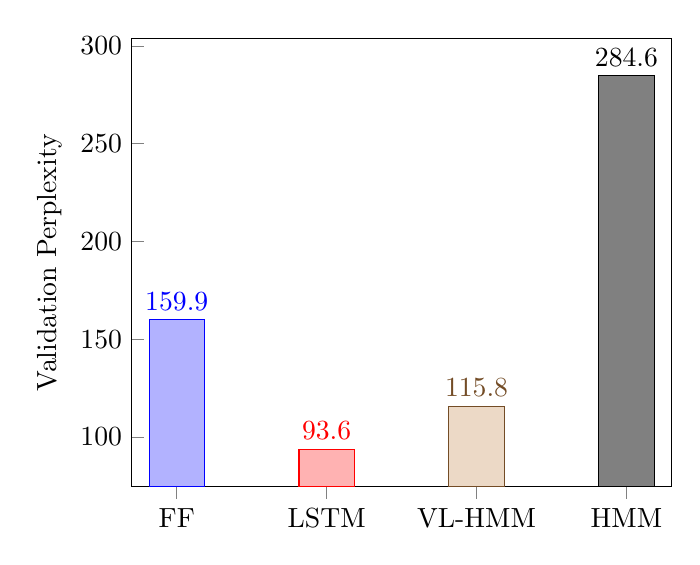
\begin{tikzpicture}
\begin{axis}[
    ybar=5pt,
    %x=4cm,
    %enlarge x limits=0.6,
    ylabel={Validation Perplexity},
    symbolic x coords={FF, LSTM, VL-HMM, HMM},
    xticklabels={FF, LSTM, VL-HMM, HMM},
    xtick={FF, LSTM, VL-HMM, HMM},
    tick pos=left,
    every axis plot/.append style={
      ybar,
      bar shift=0pt,
      fill
    },
    nodes near coords,
    nodes near coords align={vertical},
    bar width=2em,
    ]

\addplot coordinates {(FF,159.9)};
\addplot coordinates {(LSTM,93.6)};
\addplot coordinates {(VL-HMM,115.8)};
\addplot coordinates {(HMM,284.6)};

\end{axis}
\end{tikzpicture}
\end{frame}

\begin{frame}
\frametitle{State Size Ablation}

\centering
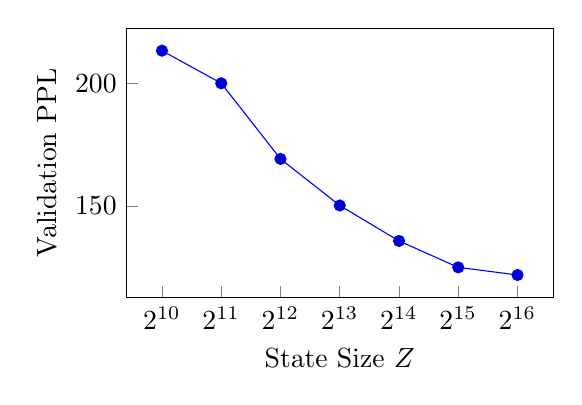
\begin{tikzpicture}
\begin{axis}[
    xlabel=State Size $Z$,
    ylabel=Validation PPL,
    xmode=log,
    log basis x={2},
    xtick={},
    tick pos=left,
    width=7cm,
    height=5cm
]
\addplot plot coordinates {
(1024,  213.25)
(2048,  199.98)
(4096,  169.18)
(8192,  150.22)
(16384, 135.79)
(32768, 125.02)
(65536, 121.93)
};
\end{axis}
\end{tikzpicture}

\vspace{2em}

Validation perplexity on PTB by state size ($\lambda =0.5$ and $M=128$)
\end{frame}

\begin{frame}
\frametitle{Other Ablations}

\begin{center}
\begin{tabular}{lrrr}
\toprule
Model                 & Param & Train & Val\\
\midrule
VL-HMM ($2^{14}$)     & 7.2M & 115    & 134 \\
\quad - neural param  & 423M & 119    & 169 \\
\quad - state dropout & 7.2M & 88     & 157 \\
\bottomrule
\end{tabular}
\end{center}
\end{frame}

\section{Scaling HMMs with Kernel Methods}

\begin{frame}
\frametitle{Embedded Structure Prediction}
\begin{itemize}
\item The previous model relied on emission sparsity constraints
\vspace{2em}
\item Can we scale with weaker assumptions?
\vspace{2em}
\item Reduce the quadratic dependence of inference on number of states
    to linear with kernel trick
\end{itemize}
\end{frame}

\begin{frame}
\frametitle{Generalized Softmax}
Focusing on the transition distribution,
\vspace{1em}
\begin{itemize}
\item Softmax
$$p(z_t \mid z_{t-1}) = \frac{\exp(\bu_{z_{t-1}}^\top \bv_{z_{t}})}
{\sum_z \exp(\bu_{z_{t-1}}^\top \bv_z)}$$
\vspace{1em}
\item Generalized Softmax
$$p(z_t \mid z_{t-1})
= \frac{K(\bu, \bv)}{\sum_z K(\bu,\bv_z)}
= \frac{\phi(\bu)^\top\phi(\bv)}
    {\sum_z \phi(\bu)^\top\phi(\bv_z)},$$
for positive kernel $K:\R^d\times\R^d\to\R_+$
and feature map $\phi:\R^d\to\R^f$
\end{itemize}
\end{frame}

\begin{frame}
\frametitle{Inference}
\begin{itemize}
\item The key $O(Z^2)$ step in the forward algorithm:
$$
p(z_t \mid x_{<t}) = \sum_{z_{t-1}} p(z_t \mid z_{t-1})p(z_{t-1} \mid x_{<t})
$$
\vspace{1em}
\item In matrix form, 
\begin{equation*}
\bm\gamma_t = \underbrace{\bm\alpha_{t-1}}_{\R^Z}\underbrace{\Lambda_{}}_{\R^{Z \times Z}},
\end{equation*}
where we have the probability of the
\begin{align*}
&\textnormal{current state } & [\bm\gamma_{t}]_{z_{t}} &= p(z_{t} \mid x_{< t}),\\
&\textnormal{last state } & [\bm\alpha_{t-1}]_{z_{t-1}} &= p(z_{t-1} \mid x_{< t}),\\
&\textnormal{transition probability } & [\Lambda]_{z_{t-1},z_t} &= p(z_t\mid z_{t-1})
\end{align*}
\end{itemize}
\end{frame}

\begin{frame}
\frametitle{Embedded Inference}
\begin{itemize}
\item Use generalized softmax in transition distribution
$$[\Lambda]_{z_{t-1},z_t} = p(z_t\mid z_{t-1}) \propto \phi(\bu_{z_{t-1}})^\top\phi(\bv_{z_t})$$
\item Allows us to apply associative property of matrix multiplication
\begin{align*}
\bm\gamma_t
&= \bm\alpha_{t-1}\Lambda\\
&= \bm\alpha_{t-1}(\textrm{diag}(d)\phi(U)\phi(V)^\top)\\
&= \underbrace{(\bm\alpha_{t-1}\circ d)}_{\R^Z}
\underbrace{\phi(U)}_{\R^{Z \times f}}
\underbrace{\phi(V)^\top}_{\R^{f \times Z}},
\end{align*}
with stacked embeddings $\phi(U),\phi(V)$
and normalizing constants $d$
\vspace{1em}
\item Takes $O(Zf)$ time from left to right!
\end{itemize}
\end{frame}

\begin{frame}
\frametitle{Experiments}
\begin{itemize}
\item Language modeling on PTB
\vspace{2em}
\item Work directly with feature map $\phi(\bx) = \exp\left(W\bx - \frac{\|x\|^2}{2}\right)$,
with learned $W\in\R^{d \times f}$
\vspace{2em}
\item No dropout or sparsity constraints
\end{itemize}
\end{frame}

\begin{comment}
\begin{frame}
\frametitle{Results on PTB Validation}
\centering
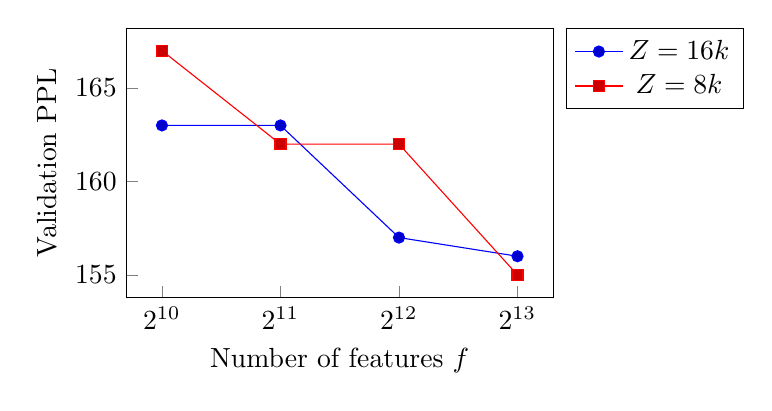
\begin{tikzpicture}
\begin{axis}[
    xlabel=Number of features $f$,
    ylabel=Validation PPL,
    xmode=log,
    log basis x={2},
    xtick={},
    tick pos=left,
    width=7cm,
    height=5cm,
    legend pos=outer north east
]
\addplot plot coordinates {
(1024,  163)
(2048,  163)
(4096,  157)
(8192,  156)
};
\addplot plot coordinates {
(1024,  167)
(2048,  162)
(4096,  162)
(8192,  155)
};
\legend{$Z=16k$,$Z=8k$}
\end{axis}
\end{tikzpicture}
\end{frame}
\end{comment}

\begin{comment}
\begin{frame}
\frametitle{Results on PTB Validation}
\centering
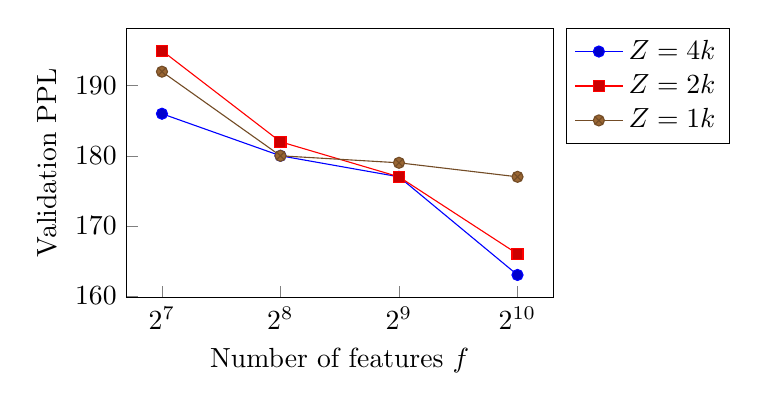
\begin{tikzpicture}
\begin{axis}[
    xlabel=Number of features $f$,
    ylabel=Validation PPL,
    xmode=log,
    log basis x={2},
    xtick={},
    tick pos=left,
    width=7cm,
    height=5cm,
    legend pos=outer north east
]
\addplot plot coordinates {
(128,  186)
(256,  180)
(512,  177)
(1024,  163)
};
\addplot plot coordinates {
(128,  195)
(256,  182)
(512,  177)
(1024,  166)
};
\addplot plot coordinates {
(128,  192)
(256,  180)
(512,  179)
(1024,  177)
};
\legend{$Z=4k$,$Z=2k$,$Z=1k$}
\end{axis}
\end{tikzpicture}
\end{frame}
\end{comment}

\begin{frame}
\frametitle{Results on PTB Validation}
\centering
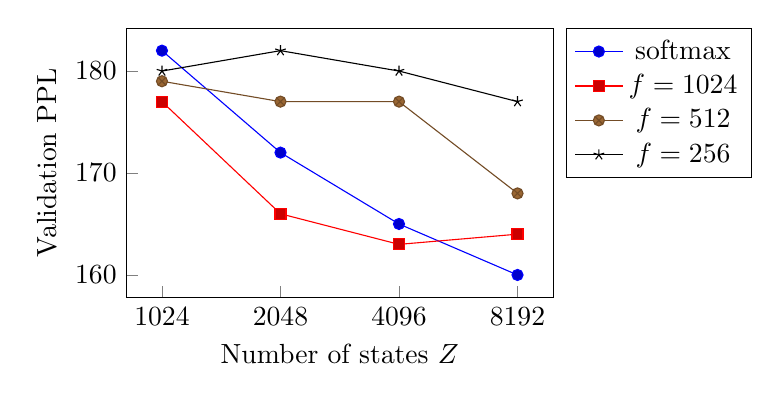
\begin{tikzpicture}
\begin{axis}[
    xlabel=Number of states $Z$,
    ylabel=Validation PPL,
    xmode=log,
    log basis x={2},
    xtick=data,
    xticklabels={1024,2048,4096,8192},
    tick pos=left,
    width=7cm,
    height=5cm,
    legend pos=outer north east
]
\addplot plot coordinates {
(1024,  182)
(2048,  172)
(4096,  165)
(8192,  160)
};
\addplot plot coordinates {
(1024,  177)
(2048,  166)
(4096,  163)
(8192,  164)
};
\addplot plot coordinates {
(1024,  179)
(2048,  177)
(4096,  177)
(8192,  168)
};
\addplot plot coordinates {
(1024,  180)
(2048,  182)
(4096,  180)
(8192,  177)
};
%\addplot plot coordinates {
%(1024,  192)
%(2048,  195)
%(4096,  186)
%(8192,  191)
%};
\legend{softmax,$f=1024$,$f=512$,$f=256$}
%\legend{softmax,$f=1024$,$f=512$,$f=256$,$f=128$}
\end{axis}
\end{tikzpicture}
\vspace{1em}
\begin{itemize}
    \item Holding number of features fixed, perplexity mostly improves
        or remains the same with an increasing number of states
    \item Achieve similar performance as softmax with around 4:1 state to feature ratio
        (also holds for 8k and 16k states)
    %\item Results are a bit noisy, hoping dropout will clean things up
    %\item Currently running that plus larger state sizes
\end{itemize}
\end{frame}

\begin{frame}
\frametitle{Conclusion}
\begin{itemize}
\item Hopeful that HMMs can be competitive language models
\vspace{2em}
\item Introduced 4 techniques for tackling speed and overfitting
\vspace{2em}
\item Future work will extend to other discrete latent variable models
\end{itemize}
\end{frame}

\begin{frame}
\frametitle{EOS}
\end{frame}


\begin{frame}
\frametitle{Citations}
\bibliographystyle{acl_natbib}
\bibliography{anthology,emnlp2020}
\end{frame}

\end{document}
